\documentclass[twoside]{book}

% Packages required by doxygen
\usepackage{fixltx2e}
\usepackage{calc}
\usepackage{doxygen}
\usepackage[export]{adjustbox} % also loads graphicx
\usepackage{graphicx}
\usepackage[utf8]{inputenc}
\usepackage{makeidx}
\usepackage{multicol}
\usepackage{multirow}
\PassOptionsToPackage{warn}{textcomp}
\usepackage{textcomp}
\usepackage[nointegrals]{wasysym}
\usepackage[table]{xcolor}

% Font selection
\usepackage[T1]{fontenc}
\usepackage[scaled=.90]{helvet}
\usepackage{courier}
\usepackage{amssymb}
\usepackage{sectsty}
\renewcommand{\familydefault}{\sfdefault}
\allsectionsfont{%
  \fontseries{bc}\selectfont%
  \color{darkgray}%
}
\renewcommand{\DoxyLabelFont}{%
  \fontseries{bc}\selectfont%
  \color{darkgray}%
}
\newcommand{\+}{\discretionary{\mbox{\scriptsize$\hookleftarrow$}}{}{}}

% Page & text layout
\usepackage{geometry}
\geometry{%
  a4paper,%
  top=2.5cm,%
  bottom=2.5cm,%
  left=2.5cm,%
  right=2.5cm%
}
\tolerance=750
\hfuzz=15pt
\hbadness=750
\setlength{\emergencystretch}{15pt}
\setlength{\parindent}{0cm}
\setlength{\parskip}{3ex plus 2ex minus 2ex}
\makeatletter
\renewcommand{\paragraph}{%
  \@startsection{paragraph}{4}{0ex}{-1.0ex}{1.0ex}{%
    \normalfont\normalsize\bfseries\SS@parafont%
  }%
}
\renewcommand{\subparagraph}{%
  \@startsection{subparagraph}{5}{0ex}{-1.0ex}{1.0ex}{%
    \normalfont\normalsize\bfseries\SS@subparafont%
  }%
}
\makeatother

% Headers & footers
\usepackage{fancyhdr}
\pagestyle{fancyplain}
\fancyhead[LE]{\fancyplain{}{\bfseries\thepage}}
\fancyhead[CE]{\fancyplain{}{}}
\fancyhead[RE]{\fancyplain{}{\bfseries\leftmark}}
\fancyhead[LO]{\fancyplain{}{\bfseries\rightmark}}
\fancyhead[CO]{\fancyplain{}{}}
\fancyhead[RO]{\fancyplain{}{\bfseries\thepage}}
\fancyfoot[LE]{\fancyplain{}{}}
\fancyfoot[CE]{\fancyplain{}{}}
\fancyfoot[RE]{\fancyplain{}{\bfseries\scriptsize Generated by Doxygen }}
\fancyfoot[LO]{\fancyplain{}{\bfseries\scriptsize Generated by Doxygen }}
\fancyfoot[CO]{\fancyplain{}{}}
\fancyfoot[RO]{\fancyplain{}{}}
\renewcommand{\footrulewidth}{0.4pt}
\renewcommand{\chaptermark}[1]{%
  \markboth{#1}{}%
}
\renewcommand{\sectionmark}[1]{%
  \markright{\thesection\ #1}%
}

% Indices & bibliography
\usepackage{natbib}
\usepackage[titles]{tocloft}
\setcounter{tocdepth}{3}
\setcounter{secnumdepth}{5}
\makeindex

% Hyperlinks (required, but should be loaded last)
\usepackage{ifpdf}
\ifpdf
  \usepackage[pdftex,pagebackref=true]{hyperref}
\else
  \usepackage[ps2pdf,pagebackref=true]{hyperref}
\fi
\hypersetup{%
  colorlinks=true,%
  linkcolor=blue,%
  citecolor=blue,%
  unicode%
}

% Custom commands
\newcommand{\clearemptydoublepage}{%
  \newpage{\pagestyle{empty}\cleardoublepage}%
}

\usepackage{caption}
\captionsetup{labelsep=space,justification=centering,font={bf},singlelinecheck=off,skip=4pt,position=top}

%===== C O N T E N T S =====

\begin{document}

% Titlepage & ToC
\hypersetup{pageanchor=false,
             bookmarksnumbered=true,
             pdfencoding=unicode
            }
\pagenumbering{roman}
\begin{titlepage}
\vspace*{7cm}
\begin{center}%
{\Large Distributed Trees \\[1ex]\large 1 }\\
\vspace*{1cm}
{\large Generated by Doxygen 1.8.11}\\
\end{center}
\end{titlepage}
\clearemptydoublepage
\tableofcontents
\clearemptydoublepage
\pagenumbering{arabic}
\hypersetup{pageanchor=true}

%--- Begin generated contents ---
\chapter{Namespace Index}
\section{Namespace List}
Here is a list of all namespaces with brief descriptions\+:\begin{DoxyCompactList}
\item\contentsline{section}{\hyperlink{namespacerdf}{rdf} }{\pageref{namespacerdf}}{}
\item\contentsline{section}{\hyperlink{namespacerdf_1_1bpc}{rdf\+::bpc} }{\pageref{namespacerdf_1_1bpc}}{}
\end{DoxyCompactList}

\chapter{Hierarchical Index}
\section{Class Hierarchy}
This inheritance list is sorted roughly, but not completely, alphabetically\+:\begin{DoxyCompactList}
\item \contentsline{section}{rdf\+:\+:bpc\+:\+:Best\+Feature\+Msg}{\pageref{classrdf_1_1bpc_1_1BestFeatureMsg}}{}
\item \contentsline{section}{rdf\+:\+:Cell}{\pageref{classrdf_1_1Cell}}{}
\begin{DoxyCompactList}
\item \contentsline{section}{rdf\+:\+:bpc\+:\+:Cell}{\pageref{classrdf_1_1bpc_1_1Cell}}{}
\end{DoxyCompactList}
\item \contentsline{section}{Collection}{\pageref{classCollection}}{}
\item \contentsline{section}{Config\+Data}{\pageref{classConfigData}}{}
\item \contentsline{section}{Config\+Validation\+Interface}{\pageref{classConfigValidationInterface}}{}
\begin{DoxyCompactList}
\item \contentsline{section}{user\+Validator}{\pageref{classuserValidator}}{}
\end{DoxyCompactList}
\item \contentsline{section}{Estructura\+:\+:Data\+Master}{\pageref{structEstructura_1_1DataMaster}}{}
\item \contentsline{section}{rdf\+:\+:Distribution\+Manager}{\pageref{classrdf_1_1DistributionManager}}{}
\item \contentsline{section}{Estructura}{\pageref{classEstructura}}{}
\item \contentsline{section}{rdf\+:\+:bpc\+:\+:Features}{\pageref{classrdf_1_1bpc_1_1Features}}{}
\item \contentsline{section}{rdf\+:\+:bpc\+:\+:Features\+Mat}{\pageref{classrdf_1_1bpc_1_1FeaturesMat}}{}
\item \contentsline{section}{rdf\+:\+:Forest\+Manager}{\pageref{classrdf_1_1ForestManager}}{}
\item \contentsline{section}{Image}{\pageref{classImage}}{}
\item \contentsline{section}{rdf\+:\+:Image\+Dispatcher}{\pageref{classrdf_1_1ImageDispatcher}}{}
\item \contentsline{section}{Image\+Getter}{\pageref{classImageGetter}}{}
\item \contentsline{section}{Image\+Manager}{\pageref{classImageManager}}{}
\item \contentsline{section}{rdf\+:\+:Image\+Operations}{\pageref{classrdf_1_1ImageOperations}}{}
\item \contentsline{section}{rdf\+:\+:Initializator}{\pageref{classrdf_1_1Initializator}}{}
\item \contentsline{section}{rdf\+:\+:Matrix$<$ T $>$}{\pageref{classrdf_1_1Matrix}}{}
\begin{DoxyCompactList}
\item \contentsline{section}{rdf\+:\+:bpc\+:\+:Matrix$<$ T $>$}{\pageref{classrdf_1_1bpc_1_1Matrix}}{}
\end{DoxyCompactList}
\item \contentsline{section}{rdf\+:\+:Matrix$<$ rdf\+:\+:bpc\+:\+:rdf\+:\+:Cell $>$}{\pageref{classrdf_1_1Matrix}}{}
\begin{DoxyCompactList}
\item \contentsline{section}{rdf\+:\+:bpc\+:\+:Matrix$<$ rdf\+:\+:bpc\+:\+:rdf\+:\+:Cell $>$}{\pageref{classrdf_1_1bpc_1_1Matrix}}{}
\end{DoxyCompactList}
\item \contentsline{section}{Matrix\+B\+P\+C\+Features$<$ T $>$}{\pageref{classMatrixBPCFeatures}}{}
\item \contentsline{section}{Estructura\+:\+:Node}{\pageref{structEstructura_1_1Node}}{}
\item \contentsline{section}{rdf\+:\+:Node}{\pageref{classrdf_1_1Node}}{}
\begin{DoxyCompactList}
\item \contentsline{section}{rdf\+:\+:Node\+Trainee}{\pageref{classrdf_1_1NodeTrainee}}{}
\begin{DoxyCompactList}
\item \contentsline{section}{rdf\+:\+:bpc\+:\+:Node\+Trainee$<$ T $>$}{\pageref{classrdf_1_1bpc_1_1NodeTrainee}}{}
\end{DoxyCompactList}
\end{DoxyCompactList}
\item \contentsline{section}{Node\+Resource}{\pageref{classNodeResource}}{}
\item \contentsline{section}{rdf\+:\+:Node\+Result}{\pageref{classrdf_1_1NodeResult}}{}
\item \contentsline{section}{Estructura\+:\+:Pixel}{\pageref{structEstructura_1_1Pixel}}{}
\item \contentsline{section}{Points\+Select}{\pageref{classPointsSelect}}{}
\item \contentsline{section}{Queue\+Task\+:\+:Queue}{\pageref{structQueueTask_1_1Queue}}{}
\item \contentsline{section}{Queue\+Task}{\pageref{classQueueTask}}{}
\item \contentsline{section}{Queue\+Thread}{\pageref{classQueueThread}}{}
\item \contentsline{section}{rdf\+:\+:Resource}{\pageref{classrdf_1_1Resource}}{}
\item \contentsline{section}{Resources}{\pageref{classResources}}{}
\item \contentsline{section}{Scheduler}{\pageref{classScheduler}}{}
\item \contentsline{section}{Strategy\+Image}{\pageref{classStrategyImage}}{}
\begin{DoxyCompactList}
\item \contentsline{section}{Depth\+Image}{\pageref{classDepthImage}}{}
\item \contentsline{section}{Label\+Image}{\pageref{classLabelImage}}{}
\end{DoxyCompactList}
\item \contentsline{section}{rdf\+:\+:Task}{\pageref{classrdf_1_1Task}}{}
\item \contentsline{section}{Queue\+Task\+:\+:Task\+Struct}{\pageref{structQueueTask_1_1TaskStruct}}{}
\item \contentsline{section}{rdf\+:\+:Trainer}{\pageref{classrdf_1_1Trainer}}{}
\begin{DoxyCompactList}
\item \contentsline{section}{rdf\+:\+:bpc\+:\+:Trainer}{\pageref{classrdf_1_1bpc_1_1Trainer}}{}
\end{DoxyCompactList}
\item \contentsline{section}{rdf\+:\+:Training\+Job}{\pageref{classrdf_1_1TrainingJob}}{}
\item \contentsline{section}{rdf\+:\+:Train\+Manager}{\pageref{classrdf_1_1TrainManager}}{}
\end{DoxyCompactList}

\chapter{Class Index}
\section{Class List}
Here are the classes, structs, unions and interfaces with brief descriptions\+:\begin{DoxyCompactList}
\item\contentsline{section}{\hyperlink{classrdf_1_1bpc_1_1BestFeatureMsg}{rdf\+::bpc\+::\+Best\+Feature\+Msg} }{\pageref{classrdf_1_1bpc_1_1BestFeatureMsg}}{}
\item\contentsline{section}{\hyperlink{classrdf_1_1Cell}{rdf\+::\+Cell} }{\pageref{classrdf_1_1Cell}}{}
\item\contentsline{section}{\hyperlink{classrdf_1_1bpc_1_1Cell}{rdf\+::bpc\+::\+Cell} }{\pageref{classrdf_1_1bpc_1_1Cell}}{}
\item\contentsline{section}{\hyperlink{classCollection}{Collection} }{\pageref{classCollection}}{}
\item\contentsline{section}{\hyperlink{classConfigData}{Config\+Data} }{\pageref{classConfigData}}{}
\item\contentsline{section}{\hyperlink{classConfigValidationInterface}{Config\+Validation\+Interface} }{\pageref{classConfigValidationInterface}}{}
\item\contentsline{section}{\hyperlink{structEstructura_1_1DataMaster}{Estructura\+::\+Data\+Master} }{\pageref{structEstructura_1_1DataMaster}}{}
\item\contentsline{section}{\hyperlink{classDepthImage}{Depth\+Image} }{\pageref{classDepthImage}}{}
\item\contentsline{section}{\hyperlink{classrdf_1_1DistributionManager}{rdf\+::\+Distribution\+Manager} }{\pageref{classrdf_1_1DistributionManager}}{}
\item\contentsline{section}{\hyperlink{classEstructura}{Estructura} }{\pageref{classEstructura}}{}
\item\contentsline{section}{\hyperlink{classrdf_1_1bpc_1_1Features}{rdf\+::bpc\+::\+Features} }{\pageref{classrdf_1_1bpc_1_1Features}}{}
\item\contentsline{section}{\hyperlink{classrdf_1_1bpc_1_1FeaturesMat}{rdf\+::bpc\+::\+Features\+Mat} }{\pageref{classrdf_1_1bpc_1_1FeaturesMat}}{}
\item\contentsline{section}{\hyperlink{classrdf_1_1ForestManager}{rdf\+::\+Forest\+Manager} }{\pageref{classrdf_1_1ForestManager}}{}
\item\contentsline{section}{\hyperlink{classImage}{Image} }{\pageref{classImage}}{}
\item\contentsline{section}{\hyperlink{classrdf_1_1ImageDispatcher}{rdf\+::\+Image\+Dispatcher} }{\pageref{classrdf_1_1ImageDispatcher}}{}
\item\contentsline{section}{\hyperlink{classImageGetter}{Image\+Getter} }{\pageref{classImageGetter}}{}
\item\contentsline{section}{\hyperlink{classImageManager}{Image\+Manager} }{\pageref{classImageManager}}{}
\item\contentsline{section}{\hyperlink{classrdf_1_1ImageOperations}{rdf\+::\+Image\+Operations} }{\pageref{classrdf_1_1ImageOperations}}{}
\item\contentsline{section}{\hyperlink{classrdf_1_1Initializator}{rdf\+::\+Initializator} }{\pageref{classrdf_1_1Initializator}}{}
\item\contentsline{section}{\hyperlink{classLabelImage}{Label\+Image} }{\pageref{classLabelImage}}{}
\item\contentsline{section}{\hyperlink{classrdf_1_1Matrix}{rdf\+::\+Matrix$<$ T $>$} }{\pageref{classrdf_1_1Matrix}}{}
\item\contentsline{section}{\hyperlink{classrdf_1_1bpc_1_1Matrix}{rdf\+::bpc\+::\+Matrix$<$ T $>$} }{\pageref{classrdf_1_1bpc_1_1Matrix}}{}
\item\contentsline{section}{\hyperlink{classMatrixBPCFeatures}{Matrix\+B\+P\+C\+Features$<$ T $>$} }{\pageref{classMatrixBPCFeatures}}{}
\item\contentsline{section}{\hyperlink{structEstructura_1_1Node}{Estructura\+::\+Node} }{\pageref{structEstructura_1_1Node}}{}
\item\contentsline{section}{\hyperlink{classrdf_1_1Node}{rdf\+::\+Node} }{\pageref{classrdf_1_1Node}}{}
\item\contentsline{section}{\hyperlink{classNodeResource}{Node\+Resource} }{\pageref{classNodeResource}}{}
\item\contentsline{section}{\hyperlink{classrdf_1_1NodeResult}{rdf\+::\+Node\+Result} }{\pageref{classrdf_1_1NodeResult}}{}
\item\contentsline{section}{\hyperlink{classrdf_1_1NodeTrainee}{rdf\+::\+Node\+Trainee} }{\pageref{classrdf_1_1NodeTrainee}}{}
\item\contentsline{section}{\hyperlink{classrdf_1_1bpc_1_1NodeTrainee}{rdf\+::bpc\+::\+Node\+Trainee$<$ T $>$} }{\pageref{classrdf_1_1bpc_1_1NodeTrainee}}{}
\item\contentsline{section}{\hyperlink{structEstructura_1_1Pixel}{Estructura\+::\+Pixel} }{\pageref{structEstructura_1_1Pixel}}{}
\item\contentsline{section}{\hyperlink{classPointsSelect}{Points\+Select} }{\pageref{classPointsSelect}}{}
\item\contentsline{section}{\hyperlink{structQueueTask_1_1Queue}{Queue\+Task\+::\+Queue} }{\pageref{structQueueTask_1_1Queue}}{}
\item\contentsline{section}{\hyperlink{classQueueTask}{Queue\+Task} }{\pageref{classQueueTask}}{}
\item\contentsline{section}{\hyperlink{classQueueThread}{Queue\+Thread} }{\pageref{classQueueThread}}{}
\item\contentsline{section}{\hyperlink{classrdf_1_1Resource}{rdf\+::\+Resource} }{\pageref{classrdf_1_1Resource}}{}
\item\contentsline{section}{\hyperlink{classResources}{Resources} }{\pageref{classResources}}{}
\item\contentsline{section}{\hyperlink{classScheduler}{Scheduler} }{\pageref{classScheduler}}{}
\item\contentsline{section}{\hyperlink{classStrategyImage}{Strategy\+Image} }{\pageref{classStrategyImage}}{}
\item\contentsline{section}{\hyperlink{classrdf_1_1Task}{rdf\+::\+Task} }{\pageref{classrdf_1_1Task}}{}
\item\contentsline{section}{\hyperlink{structQueueTask_1_1TaskStruct}{Queue\+Task\+::\+Task\+Struct} }{\pageref{structQueueTask_1_1TaskStruct}}{}
\item\contentsline{section}{\hyperlink{classrdf_1_1bpc_1_1Trainer}{rdf\+::bpc\+::\+Trainer} }{\pageref{classrdf_1_1bpc_1_1Trainer}}{}
\item\contentsline{section}{\hyperlink{classrdf_1_1Trainer}{rdf\+::\+Trainer} }{\pageref{classrdf_1_1Trainer}}{}
\item\contentsline{section}{\hyperlink{classrdf_1_1TrainingJob}{rdf\+::\+Training\+Job} }{\pageref{classrdf_1_1TrainingJob}}{}
\item\contentsline{section}{\hyperlink{classrdf_1_1TrainManager}{rdf\+::\+Train\+Manager} }{\pageref{classrdf_1_1TrainManager}}{}
\item\contentsline{section}{\hyperlink{classuserValidator}{user\+Validator} }{\pageref{classuserValidator}}{}
\end{DoxyCompactList}

\chapter{File Index}
\section{File List}
Here is a list of all files with brief descriptions\+:\begin{DoxyCompactList}
\item\contentsline{section}{\hyperlink{BestFeatureMsg_8cpp}{Best\+Feature\+Msg.\+cpp} }{\pageref{BestFeatureMsg_8cpp}}{}
\item\contentsline{section}{\hyperlink{BestFeatureMsg_8h}{Best\+Feature\+Msg.\+h} }{\pageref{BestFeatureMsg_8h}}{}
\item\contentsline{section}{\hyperlink{Cell_8cpp}{Cell.\+cpp} }{\pageref{Cell_8cpp}}{}
\item\contentsline{section}{\hyperlink{Cell_8h}{Cell.\+h} }{\pageref{Cell_8h}}{}
\item\contentsline{section}{\hyperlink{CellBPC_8cpp}{Cell\+B\+P\+C.\+cpp} }{\pageref{CellBPC_8cpp}}{}
\item\contentsline{section}{\hyperlink{CellBPC_8h}{Cell\+B\+P\+C.\+h} }{\pageref{CellBPC_8h}}{}
\item\contentsline{section}{\hyperlink{Collection_8cpp}{Collection.\+cpp} }{\pageref{Collection_8cpp}}{}
\item\contentsline{section}{\hyperlink{Collection_8h}{Collection.\+h} }{\pageref{Collection_8h}}{}
\item\contentsline{section}{\hyperlink{Config_8h}{Config.\+h} }{\pageref{Config_8h}}{}
\item\contentsline{section}{\hyperlink{ConfigData_8cpp}{Config\+Data.\+cpp} }{\pageref{ConfigData_8cpp}}{}
\item\contentsline{section}{\hyperlink{ConfigData_8h}{Config\+Data.\+h} }{\pageref{ConfigData_8h}}{}
\item\contentsline{section}{\hyperlink{ConfigValidationInterface_8h}{Config\+Validation\+Interface.\+h} }{\pageref{ConfigValidationInterface_8h}}{}
\item\contentsline{section}{\hyperlink{configValidator_8cpp}{config\+Validator.\+cpp} }{\pageref{configValidator_8cpp}}{}
\item\contentsline{section}{\hyperlink{DepthImage_8cpp}{Depth\+Image.\+cpp} }{\pageref{DepthImage_8cpp}}{}
\item\contentsline{section}{\hyperlink{DepthImage_8h}{Depth\+Image.\+h} }{\pageref{DepthImage_8h}}{}
\item\contentsline{section}{\hyperlink{DistributionManager_8cpp}{Distribution\+Manager.\+cpp} }{\pageref{DistributionManager_8cpp}}{}
\item\contentsline{section}{\hyperlink{DistributionManager_8h}{Distribution\+Manager.\+h} }{\pageref{DistributionManager_8h}}{}
\item\contentsline{section}{\hyperlink{Estructura_8cpp}{Estructura.\+cpp} }{\pageref{Estructura_8cpp}}{}
\item\contentsline{section}{\hyperlink{Estructura_8h}{Estructura.\+h} }{\pageref{Estructura_8h}}{}
\item\contentsline{section}{\hyperlink{Features_8cpp}{Features.\+cpp} }{\pageref{Features_8cpp}}{}
\item\contentsline{section}{\hyperlink{Features_8h}{Features.\+h} }{\pageref{Features_8h}}{}
\item\contentsline{section}{\hyperlink{FeaturesMat_8cpp}{Features\+Mat.\+cpp} }{\pageref{FeaturesMat_8cpp}}{}
\item\contentsline{section}{\hyperlink{FeaturesMat_8h}{Features\+Mat.\+h} }{\pageref{FeaturesMat_8h}}{}
\item\contentsline{section}{\hyperlink{ForestManager_8cpp}{Forest\+Manager.\+cpp} }{\pageref{ForestManager_8cpp}}{}
\item\contentsline{section}{\hyperlink{ForestManager_8h}{Forest\+Manager.\+h} }{\pageref{ForestManager_8h}}{}
\item\contentsline{section}{\hyperlink{Image_8cpp}{Image.\+cpp} }{\pageref{Image_8cpp}}{}
\item\contentsline{section}{\hyperlink{Image_8h}{Image.\+h} }{\pageref{Image_8h}}{}
\item\contentsline{section}{\hyperlink{ImageDispatcher_8cpp}{Image\+Dispatcher.\+cpp} }{\pageref{ImageDispatcher_8cpp}}{}
\item\contentsline{section}{\hyperlink{ImageDispatcher_8h}{Image\+Dispatcher.\+h} }{\pageref{ImageDispatcher_8h}}{}
\item\contentsline{section}{\hyperlink{ImageGetter_8cpp}{Image\+Getter.\+cpp} }{\pageref{ImageGetter_8cpp}}{}
\item\contentsline{section}{\hyperlink{ImageGetter_8h}{Image\+Getter.\+h} }{\pageref{ImageGetter_8h}}{}
\item\contentsline{section}{\hyperlink{ImageManager_8cpp}{Image\+Manager.\+cpp} }{\pageref{ImageManager_8cpp}}{}
\item\contentsline{section}{\hyperlink{ImageManager_8h}{Image\+Manager.\+h} }{\pageref{ImageManager_8h}}{}
\item\contentsline{section}{\hyperlink{ImageOperations_8cpp}{Image\+Operations.\+cpp} }{\pageref{ImageOperations_8cpp}}{}
\item\contentsline{section}{\hyperlink{ImageOperations_8h}{Image\+Operations.\+h} }{\pageref{ImageOperations_8h}}{}
\item\contentsline{section}{\hyperlink{Initializator_8cpp}{Initializator.\+cpp} }{\pageref{Initializator_8cpp}}{}
\item\contentsline{section}{\hyperlink{Initializator_8h}{Initializator.\+h} }{\pageref{Initializator_8h}}{}
\item\contentsline{section}{\hyperlink{LabelImage_8cpp}{Label\+Image.\+cpp} }{\pageref{LabelImage_8cpp}}{}
\item\contentsline{section}{\hyperlink{LabelImage_8h}{Label\+Image.\+h} }{\pageref{LabelImage_8h}}{}
\item\contentsline{section}{\hyperlink{main_8cpp}{main.\+cpp} }{\pageref{main_8cpp}}{}
\item\contentsline{section}{\hyperlink{Matrix_8h}{Matrix.\+h} }{\pageref{Matrix_8h}}{}
\item\contentsline{section}{\hyperlink{MatrixBPC_8h}{Matrix\+B\+P\+C.\+h} }{\pageref{MatrixBPC_8h}}{}
\item\contentsline{section}{\hyperlink{MatrixBPCFeatures_8cpp}{Matrix\+B\+P\+C\+Features.\+cpp} }{\pageref{MatrixBPCFeatures_8cpp}}{}
\item\contentsline{section}{\hyperlink{MatrixBPCFeatures_8h}{Matrix\+B\+P\+C\+Features.\+h} }{\pageref{MatrixBPCFeatures_8h}}{}
\item\contentsline{section}{\hyperlink{Node_8cpp}{Node.\+cpp} }{\pageref{Node_8cpp}}{}
\item\contentsline{section}{\hyperlink{Node_8h}{Node.\+h} }{\pageref{Node_8h}}{}
\item\contentsline{section}{\hyperlink{NodeResource_8cpp}{Node\+Resource.\+cpp} }{\pageref{NodeResource_8cpp}}{}
\item\contentsline{section}{\hyperlink{NodeResource_8h}{Node\+Resource.\+h} }{\pageref{NodeResource_8h}}{}
\item\contentsline{section}{\hyperlink{NodeResult_8cpp}{Node\+Result.\+cpp} }{\pageref{NodeResult_8cpp}}{}
\item\contentsline{section}{\hyperlink{NodeResult_8h}{Node\+Result.\+h} }{\pageref{NodeResult_8h}}{}
\item\contentsline{section}{\hyperlink{NodeTrainee_8cpp}{Node\+Trainee.\+cpp} }{\pageref{NodeTrainee_8cpp}}{}
\item\contentsline{section}{\hyperlink{NodeTrainee_8h}{Node\+Trainee.\+h} }{\pageref{NodeTrainee_8h}}{}
\item\contentsline{section}{\hyperlink{NodeTraineeBPC_8h}{Node\+Trainee\+B\+P\+C.\+h} }{\pageref{NodeTraineeBPC_8h}}{}
\item\contentsline{section}{\hyperlink{PointsSelect_8cpp}{Points\+Select.\+cpp} }{\pageref{PointsSelect_8cpp}}{}
\item\contentsline{section}{\hyperlink{PointsSelect_8h}{Points\+Select.\+h} }{\pageref{PointsSelect_8h}}{}
\item\contentsline{section}{\hyperlink{QueueTask_8cpp}{Queue\+Task.\+cpp} }{\pageref{QueueTask_8cpp}}{}
\item\contentsline{section}{\hyperlink{QueueTask_8h}{Queue\+Task.\+h} }{\pageref{QueueTask_8h}}{}
\item\contentsline{section}{\hyperlink{QueueThread_8cpp}{Queue\+Thread.\+cpp} }{\pageref{QueueThread_8cpp}}{}
\item\contentsline{section}{\hyperlink{QueueThread_8h}{Queue\+Thread.\+h} }{\pageref{QueueThread_8h}}{}
\item\contentsline{section}{\hyperlink{Resource_8cpp}{Resource.\+cpp} }{\pageref{Resource_8cpp}}{}
\item\contentsline{section}{\hyperlink{Resource_8h}{Resource.\+h} }{\pageref{Resource_8h}}{}
\item\contentsline{section}{\hyperlink{Resources_8cpp}{Resources.\+cpp} }{\pageref{Resources_8cpp}}{}
\item\contentsline{section}{\hyperlink{Resources_8h}{Resources.\+h} }{\pageref{Resources_8h}}{}
\item\contentsline{section}{\hyperlink{Scheduler_8cpp}{Scheduler.\+cpp} }{\pageref{Scheduler_8cpp}}{}
\item\contentsline{section}{\hyperlink{Scheduler_8h}{Scheduler.\+h} }{\pageref{Scheduler_8h}}{}
\item\contentsline{section}{\hyperlink{StrategyImage_8cpp}{Strategy\+Image.\+cpp} }{\pageref{StrategyImage_8cpp}}{}
\item\contentsline{section}{\hyperlink{StrategyImage_8h}{Strategy\+Image.\+h} }{\pageref{StrategyImage_8h}}{}
\item\contentsline{section}{\hyperlink{Task_8cpp}{Task.\+cpp} }{\pageref{Task_8cpp}}{}
\item\contentsline{section}{\hyperlink{Task_8h}{Task.\+h} }{\pageref{Task_8h}}{}
\item\contentsline{section}{\hyperlink{Trainer_8cpp}{Trainer.\+cpp} }{\pageref{Trainer_8cpp}}{}
\item\contentsline{section}{\hyperlink{Trainer_8h}{Trainer.\+h} }{\pageref{Trainer_8h}}{}
\item\contentsline{section}{\hyperlink{TrainerBPC_8cpp}{Trainer\+B\+P\+C.\+cpp} }{\pageref{TrainerBPC_8cpp}}{}
\item\contentsline{section}{\hyperlink{TrainerBPC_8h}{Trainer\+B\+P\+C.\+h} }{\pageref{TrainerBPC_8h}}{}
\item\contentsline{section}{\hyperlink{TrainingJob_8cpp}{Training\+Job.\+cpp} }{\pageref{TrainingJob_8cpp}}{}
\item\contentsline{section}{\hyperlink{TrainingJob_8h}{Training\+Job.\+h} }{\pageref{TrainingJob_8h}}{}
\item\contentsline{section}{\hyperlink{TrainManager_8cpp}{Train\+Manager.\+cpp} }{\pageref{TrainManager_8cpp}}{}
\item\contentsline{section}{\hyperlink{TrainManager_8h}{Train\+Manager.\+h} }{\pageref{TrainManager_8h}}{}
\item\contentsline{section}{\hyperlink{userValidator_8cpp}{user\+Validator.\+cpp} }{\pageref{userValidator_8cpp}}{}
\item\contentsline{section}{\hyperlink{userValidator_8h}{user\+Validator.\+h} }{\pageref{userValidator_8h}}{}
\end{DoxyCompactList}

\chapter{Namespace Documentation}
\hypertarget{namespacerdf}{}\section{rdf Namespace Reference}
\label{namespacerdf}\index{rdf@{rdf}}
\subsection*{Namespaces}
\begin{DoxyCompactItemize}
\item 
 \hyperlink{namespacerdf_1_1bpc}{bpc}
\end{DoxyCompactItemize}
\subsection*{Classes}
\begin{DoxyCompactItemize}
\item 
class \hyperlink{classrdf_1_1Cell}{Cell}
\item 
class \hyperlink{classrdf_1_1DistributionManager}{Distribution\+Manager}
\item 
class \hyperlink{classrdf_1_1ForestManager}{Forest\+Manager}
\item 
class \hyperlink{classrdf_1_1ImageDispatcher}{Image\+Dispatcher}
\item 
class \hyperlink{classrdf_1_1ImageOperations}{Image\+Operations}
\item 
class \hyperlink{classrdf_1_1Initializator}{Initializator}
\item 
class \hyperlink{classrdf_1_1Matrix}{Matrix}
\item 
class \hyperlink{classrdf_1_1Node}{Node}
\item 
class \hyperlink{classrdf_1_1NodeResult}{Node\+Result}
\item 
class \hyperlink{classrdf_1_1NodeTrainee}{Node\+Trainee}
\item 
class \hyperlink{classrdf_1_1Resource}{Resource}
\item 
class \hyperlink{classrdf_1_1Task}{Task}
\item 
class \hyperlink{classrdf_1_1Trainer}{Trainer}
\item 
class \hyperlink{classrdf_1_1TrainingJob}{Training\+Job}
\item 
class \hyperlink{classrdf_1_1TrainManager}{Train\+Manager}
\end{DoxyCompactItemize}

\hypertarget{namespacerdf_1_1bpc}{}\section{rdf\+:\+:bpc Namespace Reference}
\label{namespacerdf_1_1bpc}\index{rdf\+::bpc@{rdf\+::bpc}}
\subsection*{Classes}
\begin{DoxyCompactItemize}
\item 
class \hyperlink{classrdf_1_1bpc_1_1BestFeatureMsg}{Best\+Feature\+Msg}
\item 
class \hyperlink{classrdf_1_1bpc_1_1Cell}{Cell}
\item 
class \hyperlink{classrdf_1_1bpc_1_1Features}{Features}
\item 
class \hyperlink{classrdf_1_1bpc_1_1FeaturesMat}{Features\+Mat}
\item 
class \hyperlink{classrdf_1_1bpc_1_1Matrix}{Matrix}
\item 
class \hyperlink{classrdf_1_1bpc_1_1NodeTrainee}{Node\+Trainee}
\item 
class \hyperlink{classrdf_1_1bpc_1_1Trainer}{Trainer}
\end{DoxyCompactItemize}
\subsection*{Typedefs}
\begin{DoxyCompactItemize}
\item 
typedef Cv\+Point2\+D32f \hyperlink{namespacerdf_1_1bpc_a507d4ac6b23164245625d13196e564bc}{Feature}
\end{DoxyCompactItemize}


\subsection{Typedef Documentation}
\index{rdf\+::bpc@{rdf\+::bpc}!Feature@{Feature}}
\index{Feature@{Feature}!rdf\+::bpc@{rdf\+::bpc}}
\subsubsection[{\texorpdfstring{Feature}{Feature}}]{\setlength{\rightskip}{0pt plus 5cm}typedef Cv\+Point2\+D32f {\bf rdf\+::bpc\+::\+Feature}}\hypertarget{namespacerdf_1_1bpc_a507d4ac6b23164245625d13196e564bc}{}\label{namespacerdf_1_1bpc_a507d4ac6b23164245625d13196e564bc}

\chapter{Class Documentation}
\hypertarget{classrdf_1_1bpc_1_1BestFeatureMsg}{}\section{rdf\+:\+:bpc\+:\+:Best\+Feature\+Msg Class Reference}
\label{classrdf_1_1bpc_1_1BestFeatureMsg}\index{rdf\+::bpc\+::\+Best\+Feature\+Msg@{rdf\+::bpc\+::\+Best\+Feature\+Msg}}


{\ttfamily \#include $<$Best\+Feature\+Msg.\+h$>$}



Collaboration diagram for rdf\+:\+:bpc\+:\+:Best\+Feature\+Msg\+:
\nopagebreak
\begin{figure}[H]
\begin{center}
\leavevmode
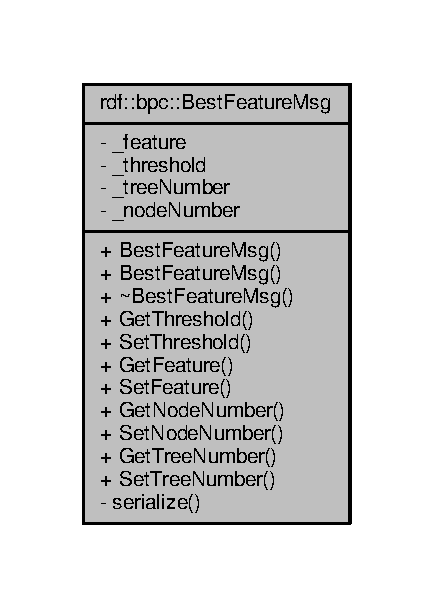
\includegraphics[width=208pt]{classrdf_1_1bpc_1_1BestFeatureMsg__coll__graph}
\end{center}
\end{figure}
\subsection*{Public Member Functions}
\begin{DoxyCompactItemize}
\item 
\hyperlink{classrdf_1_1bpc_1_1BestFeatureMsg_a6a586e4d7b8c4220176cf84ac7348a7d}{Best\+Feature\+Msg} ()
\item 
\hyperlink{classrdf_1_1bpc_1_1BestFeatureMsg_a29d3de822225c6675886108a04948d67}{Best\+Feature\+Msg} (const \hyperlink{classrdf_1_1bpc_1_1BestFeatureMsg}{Best\+Feature\+Msg} \&orig)
\item 
virtual \hyperlink{classrdf_1_1bpc_1_1BestFeatureMsg_a73780143fc64dace2584c3e91c49818b}{$\sim$\+Best\+Feature\+Msg} ()
\item 
float \hyperlink{classrdf_1_1bpc_1_1BestFeatureMsg_a62cf5b6e9c1ff7c3e17b1fa4bb6bdcf7}{Get\+Threshold} () const 
\item 
void \hyperlink{classrdf_1_1bpc_1_1BestFeatureMsg_a9099e3dfd687934a25eee58c3322e47f}{Set\+Threshold} (float \hyperlink{classrdf_1_1bpc_1_1BestFeatureMsg_aababadc862b2794ea24eb37128b2648f}{\+\_\+threshold})
\item 
\hyperlink{classrdf_1_1bpc_1_1Features}{Features} \hyperlink{classrdf_1_1bpc_1_1BestFeatureMsg_ae25e411935ae331d9427da3707bc0d2c}{Get\+Feature} () const 
\item 
void \hyperlink{classrdf_1_1bpc_1_1BestFeatureMsg_acabaf5de41b98f94265bd0582f5fd207}{Set\+Feature} (\hyperlink{classrdf_1_1bpc_1_1Features}{Features} \hyperlink{classrdf_1_1bpc_1_1BestFeatureMsg_a7b383b71e2a03d3491d1fabc810c607f}{\+\_\+feature})
\item 
int \hyperlink{classrdf_1_1bpc_1_1BestFeatureMsg_a5f92bf9cfd7009fe5478e7eefc94698f}{Get\+Node\+Number} () const 
\item 
void \hyperlink{classrdf_1_1bpc_1_1BestFeatureMsg_a0c6d0a13e6f27d6ab8c32408fadbd16d}{Set\+Node\+Number} (int \hyperlink{classrdf_1_1bpc_1_1BestFeatureMsg_a50e19bc479f97975aac7194d444d283c}{\+\_\+node\+Number})
\item 
int \hyperlink{classrdf_1_1bpc_1_1BestFeatureMsg_a1083940d56360c005916a80a2ce3612c}{Get\+Tree\+Number} () const 
\item 
void \hyperlink{classrdf_1_1bpc_1_1BestFeatureMsg_a6f2ef9783627a7d3ccf8256289c1044b}{Set\+Tree\+Number} (int \hyperlink{classrdf_1_1bpc_1_1BestFeatureMsg_a6d8b8a53e1baf9a008e0320839002728}{\+\_\+tree\+Number})
\end{DoxyCompactItemize}
\subsection*{Private Member Functions}
\begin{DoxyCompactItemize}
\item 
{\footnotesize template$<$class Archive $>$ }\\void \hyperlink{classrdf_1_1bpc_1_1BestFeatureMsg_ac869a153a4a3e3655b82a2a203655231}{serialize} (Archive \&ar, const unsigned int version)
\end{DoxyCompactItemize}
\subsection*{Private Attributes}
\begin{DoxyCompactItemize}
\item 
\hyperlink{classrdf_1_1bpc_1_1Features}{Features} \hyperlink{classrdf_1_1bpc_1_1BestFeatureMsg_a7b383b71e2a03d3491d1fabc810c607f}{\+\_\+feature}
\item 
float \hyperlink{classrdf_1_1bpc_1_1BestFeatureMsg_aababadc862b2794ea24eb37128b2648f}{\+\_\+threshold}
\item 
int \hyperlink{classrdf_1_1bpc_1_1BestFeatureMsg_a6d8b8a53e1baf9a008e0320839002728}{\+\_\+tree\+Number}
\item 
int \hyperlink{classrdf_1_1bpc_1_1BestFeatureMsg_a50e19bc479f97975aac7194d444d283c}{\+\_\+node\+Number}
\end{DoxyCompactItemize}
\subsection*{Friends}
\begin{DoxyCompactItemize}
\item 
class \hyperlink{classrdf_1_1bpc_1_1BestFeatureMsg_ac98d07dd8f7b70e16ccb9a01abf56b9c}{boost\+::serialization\+::access}
\end{DoxyCompactItemize}


\subsection{Constructor \& Destructor Documentation}
\index{rdf\+::bpc\+::\+Best\+Feature\+Msg@{rdf\+::bpc\+::\+Best\+Feature\+Msg}!Best\+Feature\+Msg@{Best\+Feature\+Msg}}
\index{Best\+Feature\+Msg@{Best\+Feature\+Msg}!rdf\+::bpc\+::\+Best\+Feature\+Msg@{rdf\+::bpc\+::\+Best\+Feature\+Msg}}
\subsubsection[{\texorpdfstring{Best\+Feature\+Msg()}{BestFeatureMsg()}}]{\setlength{\rightskip}{0pt plus 5cm}rdf\+::bpc\+::\+Best\+Feature\+Msg\+::\+Best\+Feature\+Msg (
\begin{DoxyParamCaption}
{}
\end{DoxyParamCaption}
)}\hypertarget{classrdf_1_1bpc_1_1BestFeatureMsg_a6a586e4d7b8c4220176cf84ac7348a7d}{}\label{classrdf_1_1bpc_1_1BestFeatureMsg_a6a586e4d7b8c4220176cf84ac7348a7d}

\begin{DoxyCode}
16                                      \{
17 \}
\end{DoxyCode}
\index{rdf\+::bpc\+::\+Best\+Feature\+Msg@{rdf\+::bpc\+::\+Best\+Feature\+Msg}!Best\+Feature\+Msg@{Best\+Feature\+Msg}}
\index{Best\+Feature\+Msg@{Best\+Feature\+Msg}!rdf\+::bpc\+::\+Best\+Feature\+Msg@{rdf\+::bpc\+::\+Best\+Feature\+Msg}}
\subsubsection[{\texorpdfstring{Best\+Feature\+Msg(const Best\+Feature\+Msg \&orig)}{BestFeatureMsg(const BestFeatureMsg &orig)}}]{\setlength{\rightskip}{0pt plus 5cm}rdf\+::bpc\+::\+Best\+Feature\+Msg\+::\+Best\+Feature\+Msg (
\begin{DoxyParamCaption}
\item[{const {\bf Best\+Feature\+Msg} \&}]{orig}
\end{DoxyParamCaption}
)}\hypertarget{classrdf_1_1bpc_1_1BestFeatureMsg_a29d3de822225c6675886108a04948d67}{}\label{classrdf_1_1bpc_1_1BestFeatureMsg_a29d3de822225c6675886108a04948d67}

\begin{DoxyCode}
19                                                                \{
20 \}
\end{DoxyCode}
\index{rdf\+::bpc\+::\+Best\+Feature\+Msg@{rdf\+::bpc\+::\+Best\+Feature\+Msg}!````~Best\+Feature\+Msg@{$\sim$\+Best\+Feature\+Msg}}
\index{````~Best\+Feature\+Msg@{$\sim$\+Best\+Feature\+Msg}!rdf\+::bpc\+::\+Best\+Feature\+Msg@{rdf\+::bpc\+::\+Best\+Feature\+Msg}}
\subsubsection[{\texorpdfstring{$\sim$\+Best\+Feature\+Msg()}{~BestFeatureMsg()}}]{\setlength{\rightskip}{0pt plus 5cm}rdf\+::bpc\+::\+Best\+Feature\+Msg\+::$\sim$\+Best\+Feature\+Msg (
\begin{DoxyParamCaption}
{}
\end{DoxyParamCaption}
)\hspace{0.3cm}{\ttfamily [virtual]}}\hypertarget{classrdf_1_1bpc_1_1BestFeatureMsg_a73780143fc64dace2584c3e91c49818b}{}\label{classrdf_1_1bpc_1_1BestFeatureMsg_a73780143fc64dace2584c3e91c49818b}

\begin{DoxyCode}
22                                       \{
23 \}
\end{DoxyCode}


\subsection{Member Function Documentation}
\index{rdf\+::bpc\+::\+Best\+Feature\+Msg@{rdf\+::bpc\+::\+Best\+Feature\+Msg}!Get\+Feature@{Get\+Feature}}
\index{Get\+Feature@{Get\+Feature}!rdf\+::bpc\+::\+Best\+Feature\+Msg@{rdf\+::bpc\+::\+Best\+Feature\+Msg}}
\subsubsection[{\texorpdfstring{Get\+Feature() const }{GetFeature() const }}]{\setlength{\rightskip}{0pt plus 5cm}{\bf Features} rdf\+::bpc\+::\+Best\+Feature\+Msg\+::\+Get\+Feature (
\begin{DoxyParamCaption}
{}
\end{DoxyParamCaption}
) const\hspace{0.3cm}{\ttfamily [inline]}}\hypertarget{classrdf_1_1bpc_1_1BestFeatureMsg_ae25e411935ae331d9427da3707bc0d2c}{}\label{classrdf_1_1bpc_1_1BestFeatureMsg_ae25e411935ae331d9427da3707bc0d2c}


References \+\_\+feature.


\begin{DoxyCode}
37                                         \{
38                 \textcolor{keywordflow}{return} \hyperlink{classrdf_1_1bpc_1_1BestFeatureMsg_a7b383b71e2a03d3491d1fabc810c607f}{\_feature};
39             \}
\end{DoxyCode}
\index{rdf\+::bpc\+::\+Best\+Feature\+Msg@{rdf\+::bpc\+::\+Best\+Feature\+Msg}!Get\+Node\+Number@{Get\+Node\+Number}}
\index{Get\+Node\+Number@{Get\+Node\+Number}!rdf\+::bpc\+::\+Best\+Feature\+Msg@{rdf\+::bpc\+::\+Best\+Feature\+Msg}}
\subsubsection[{\texorpdfstring{Get\+Node\+Number() const }{GetNodeNumber() const }}]{\setlength{\rightskip}{0pt plus 5cm}int rdf\+::bpc\+::\+Best\+Feature\+Msg\+::\+Get\+Node\+Number (
\begin{DoxyParamCaption}
{}
\end{DoxyParamCaption}
) const\hspace{0.3cm}{\ttfamily [inline]}}\hypertarget{classrdf_1_1bpc_1_1BestFeatureMsg_a5f92bf9cfd7009fe5478e7eefc94698f}{}\label{classrdf_1_1bpc_1_1BestFeatureMsg_a5f92bf9cfd7009fe5478e7eefc94698f}


References \+\_\+node\+Number.


\begin{DoxyCode}
45                                       \{
46                 \textcolor{keywordflow}{return} \hyperlink{classrdf_1_1bpc_1_1BestFeatureMsg_a50e19bc479f97975aac7194d444d283c}{\_nodeNumber};
47             \}
\end{DoxyCode}
\index{rdf\+::bpc\+::\+Best\+Feature\+Msg@{rdf\+::bpc\+::\+Best\+Feature\+Msg}!Get\+Threshold@{Get\+Threshold}}
\index{Get\+Threshold@{Get\+Threshold}!rdf\+::bpc\+::\+Best\+Feature\+Msg@{rdf\+::bpc\+::\+Best\+Feature\+Msg}}
\subsubsection[{\texorpdfstring{Get\+Threshold() const }{GetThreshold() const }}]{\setlength{\rightskip}{0pt plus 5cm}float rdf\+::bpc\+::\+Best\+Feature\+Msg\+::\+Get\+Threshold (
\begin{DoxyParamCaption}
{}
\end{DoxyParamCaption}
) const\hspace{0.3cm}{\ttfamily [inline]}}\hypertarget{classrdf_1_1bpc_1_1BestFeatureMsg_a62cf5b6e9c1ff7c3e17b1fa4bb6bdcf7}{}\label{classrdf_1_1bpc_1_1BestFeatureMsg_a62cf5b6e9c1ff7c3e17b1fa4bb6bdcf7}


References \+\_\+threshold.


\begin{DoxyCode}
30                                        \{
31                 \textcolor{keywordflow}{return} \hyperlink{classrdf_1_1bpc_1_1BestFeatureMsg_aababadc862b2794ea24eb37128b2648f}{\_threshold};
32             \}
\end{DoxyCode}
\index{rdf\+::bpc\+::\+Best\+Feature\+Msg@{rdf\+::bpc\+::\+Best\+Feature\+Msg}!Get\+Tree\+Number@{Get\+Tree\+Number}}
\index{Get\+Tree\+Number@{Get\+Tree\+Number}!rdf\+::bpc\+::\+Best\+Feature\+Msg@{rdf\+::bpc\+::\+Best\+Feature\+Msg}}
\subsubsection[{\texorpdfstring{Get\+Tree\+Number() const }{GetTreeNumber() const }}]{\setlength{\rightskip}{0pt plus 5cm}int rdf\+::bpc\+::\+Best\+Feature\+Msg\+::\+Get\+Tree\+Number (
\begin{DoxyParamCaption}
{}
\end{DoxyParamCaption}
) const\hspace{0.3cm}{\ttfamily [inline]}}\hypertarget{classrdf_1_1bpc_1_1BestFeatureMsg_a1083940d56360c005916a80a2ce3612c}{}\label{classrdf_1_1bpc_1_1BestFeatureMsg_a1083940d56360c005916a80a2ce3612c}


References \+\_\+tree\+Number.


\begin{DoxyCode}
53                                       \{
54                 \textcolor{keywordflow}{return} \hyperlink{classrdf_1_1bpc_1_1BestFeatureMsg_a6d8b8a53e1baf9a008e0320839002728}{\_treeNumber};
55             \}
\end{DoxyCode}
\index{rdf\+::bpc\+::\+Best\+Feature\+Msg@{rdf\+::bpc\+::\+Best\+Feature\+Msg}!serialize@{serialize}}
\index{serialize@{serialize}!rdf\+::bpc\+::\+Best\+Feature\+Msg@{rdf\+::bpc\+::\+Best\+Feature\+Msg}}
\subsubsection[{\texorpdfstring{serialize(\+Archive \&ar, const unsigned int version)}{serialize(Archive &ar, const unsigned int version)}}]{\setlength{\rightskip}{0pt plus 5cm}template$<$class Archive $>$ void rdf\+::bpc\+::\+Best\+Feature\+Msg\+::serialize (
\begin{DoxyParamCaption}
\item[{Archive \&}]{ar, }
\item[{const unsigned int}]{version}
\end{DoxyParamCaption}
)\hspace{0.3cm}{\ttfamily [inline]}, {\ttfamily [private]}}\hypertarget{classrdf_1_1bpc_1_1BestFeatureMsg_ac869a153a4a3e3655b82a2a203655231}{}\label{classrdf_1_1bpc_1_1BestFeatureMsg_ac869a153a4a3e3655b82a2a203655231}


References \+\_\+feature, \+\_\+node\+Number, \+\_\+threshold, and \+\_\+tree\+Number.


\begin{DoxyCode}
66             \{
67                 ar & \hyperlink{classrdf_1_1bpc_1_1BestFeatureMsg_a7b383b71e2a03d3491d1fabc810c607f}{\_feature};
68                 ar & \hyperlink{classrdf_1_1bpc_1_1BestFeatureMsg_aababadc862b2794ea24eb37128b2648f}{\_threshold};
69                 ar & \hyperlink{classrdf_1_1bpc_1_1BestFeatureMsg_a6d8b8a53e1baf9a008e0320839002728}{\_treeNumber};
70                 ar & \hyperlink{classrdf_1_1bpc_1_1BestFeatureMsg_a50e19bc479f97975aac7194d444d283c}{\_nodeNumber};
71             \}
\end{DoxyCode}
\index{rdf\+::bpc\+::\+Best\+Feature\+Msg@{rdf\+::bpc\+::\+Best\+Feature\+Msg}!Set\+Feature@{Set\+Feature}}
\index{Set\+Feature@{Set\+Feature}!rdf\+::bpc\+::\+Best\+Feature\+Msg@{rdf\+::bpc\+::\+Best\+Feature\+Msg}}
\subsubsection[{\texorpdfstring{Set\+Feature(\+Features \+\_\+feature)}{SetFeature(Features _feature)}}]{\setlength{\rightskip}{0pt plus 5cm}void rdf\+::bpc\+::\+Best\+Feature\+Msg\+::\+Set\+Feature (
\begin{DoxyParamCaption}
\item[{{\bf Features}}]{\+\_\+feature}
\end{DoxyParamCaption}
)\hspace{0.3cm}{\ttfamily [inline]}}\hypertarget{classrdf_1_1bpc_1_1BestFeatureMsg_acabaf5de41b98f94265bd0582f5fd207}{}\label{classrdf_1_1bpc_1_1BestFeatureMsg_acabaf5de41b98f94265bd0582f5fd207}


References \+\_\+feature.


\begin{DoxyCode}
41                                                \{
42                 this->\hyperlink{classrdf_1_1bpc_1_1BestFeatureMsg_a7b383b71e2a03d3491d1fabc810c607f}{\_feature} = \hyperlink{classrdf_1_1bpc_1_1BestFeatureMsg_a7b383b71e2a03d3491d1fabc810c607f}{\_feature};
43             \}
\end{DoxyCode}
\index{rdf\+::bpc\+::\+Best\+Feature\+Msg@{rdf\+::bpc\+::\+Best\+Feature\+Msg}!Set\+Node\+Number@{Set\+Node\+Number}}
\index{Set\+Node\+Number@{Set\+Node\+Number}!rdf\+::bpc\+::\+Best\+Feature\+Msg@{rdf\+::bpc\+::\+Best\+Feature\+Msg}}
\subsubsection[{\texorpdfstring{Set\+Node\+Number(int \+\_\+node\+Number)}{SetNodeNumber(int _nodeNumber)}}]{\setlength{\rightskip}{0pt plus 5cm}void rdf\+::bpc\+::\+Best\+Feature\+Msg\+::\+Set\+Node\+Number (
\begin{DoxyParamCaption}
\item[{int}]{\+\_\+node\+Number}
\end{DoxyParamCaption}
)\hspace{0.3cm}{\ttfamily [inline]}}\hypertarget{classrdf_1_1bpc_1_1BestFeatureMsg_a0c6d0a13e6f27d6ab8c32408fadbd16d}{}\label{classrdf_1_1bpc_1_1BestFeatureMsg_a0c6d0a13e6f27d6ab8c32408fadbd16d}


References \+\_\+node\+Number.


\begin{DoxyCode}
49                                                 \{
50                 this->\hyperlink{classrdf_1_1bpc_1_1BestFeatureMsg_a50e19bc479f97975aac7194d444d283c}{\_nodeNumber} = \hyperlink{classrdf_1_1bpc_1_1BestFeatureMsg_a50e19bc479f97975aac7194d444d283c}{\_nodeNumber};
51             \}
\end{DoxyCode}
\index{rdf\+::bpc\+::\+Best\+Feature\+Msg@{rdf\+::bpc\+::\+Best\+Feature\+Msg}!Set\+Threshold@{Set\+Threshold}}
\index{Set\+Threshold@{Set\+Threshold}!rdf\+::bpc\+::\+Best\+Feature\+Msg@{rdf\+::bpc\+::\+Best\+Feature\+Msg}}
\subsubsection[{\texorpdfstring{Set\+Threshold(float \+\_\+threshold)}{SetThreshold(float _threshold)}}]{\setlength{\rightskip}{0pt plus 5cm}void rdf\+::bpc\+::\+Best\+Feature\+Msg\+::\+Set\+Threshold (
\begin{DoxyParamCaption}
\item[{float}]{\+\_\+threshold}
\end{DoxyParamCaption}
)\hspace{0.3cm}{\ttfamily [inline]}}\hypertarget{classrdf_1_1bpc_1_1BestFeatureMsg_a9099e3dfd687934a25eee58c3322e47f}{}\label{classrdf_1_1bpc_1_1BestFeatureMsg_a9099e3dfd687934a25eee58c3322e47f}


References \+\_\+threshold.


\begin{DoxyCode}
34                                                 \{
35                 this->\hyperlink{classrdf_1_1bpc_1_1BestFeatureMsg_aababadc862b2794ea24eb37128b2648f}{\_threshold} = \hyperlink{classrdf_1_1bpc_1_1BestFeatureMsg_aababadc862b2794ea24eb37128b2648f}{\_threshold};
36             \}
\end{DoxyCode}
\index{rdf\+::bpc\+::\+Best\+Feature\+Msg@{rdf\+::bpc\+::\+Best\+Feature\+Msg}!Set\+Tree\+Number@{Set\+Tree\+Number}}
\index{Set\+Tree\+Number@{Set\+Tree\+Number}!rdf\+::bpc\+::\+Best\+Feature\+Msg@{rdf\+::bpc\+::\+Best\+Feature\+Msg}}
\subsubsection[{\texorpdfstring{Set\+Tree\+Number(int \+\_\+tree\+Number)}{SetTreeNumber(int _treeNumber)}}]{\setlength{\rightskip}{0pt plus 5cm}void rdf\+::bpc\+::\+Best\+Feature\+Msg\+::\+Set\+Tree\+Number (
\begin{DoxyParamCaption}
\item[{int}]{\+\_\+tree\+Number}
\end{DoxyParamCaption}
)\hspace{0.3cm}{\ttfamily [inline]}}\hypertarget{classrdf_1_1bpc_1_1BestFeatureMsg_a6f2ef9783627a7d3ccf8256289c1044b}{}\label{classrdf_1_1bpc_1_1BestFeatureMsg_a6f2ef9783627a7d3ccf8256289c1044b}


References \+\_\+tree\+Number.


\begin{DoxyCode}
57                                                 \{
58                 this->\hyperlink{classrdf_1_1bpc_1_1BestFeatureMsg_a6d8b8a53e1baf9a008e0320839002728}{\_treeNumber} = \hyperlink{classrdf_1_1bpc_1_1BestFeatureMsg_a6d8b8a53e1baf9a008e0320839002728}{\_treeNumber};
59             \}
\end{DoxyCode}


\subsection{Friends And Related Function Documentation}
\index{rdf\+::bpc\+::\+Best\+Feature\+Msg@{rdf\+::bpc\+::\+Best\+Feature\+Msg}!boost\+::serialization\+::access@{boost\+::serialization\+::access}}
\index{boost\+::serialization\+::access@{boost\+::serialization\+::access}!rdf\+::bpc\+::\+Best\+Feature\+Msg@{rdf\+::bpc\+::\+Best\+Feature\+Msg}}
\subsubsection[{\texorpdfstring{boost\+::serialization\+::access}{boost::serialization::access}}]{\setlength{\rightskip}{0pt plus 5cm}friend class boost\+::serialization\+::access\hspace{0.3cm}{\ttfamily [friend]}}\hypertarget{classrdf_1_1bpc_1_1BestFeatureMsg_ac98d07dd8f7b70e16ccb9a01abf56b9c}{}\label{classrdf_1_1bpc_1_1BestFeatureMsg_ac98d07dd8f7b70e16ccb9a01abf56b9c}


\subsection{Member Data Documentation}
\index{rdf\+::bpc\+::\+Best\+Feature\+Msg@{rdf\+::bpc\+::\+Best\+Feature\+Msg}!\+\_\+feature@{\+\_\+feature}}
\index{\+\_\+feature@{\+\_\+feature}!rdf\+::bpc\+::\+Best\+Feature\+Msg@{rdf\+::bpc\+::\+Best\+Feature\+Msg}}
\subsubsection[{\texorpdfstring{\+\_\+feature}{_feature}}]{\setlength{\rightskip}{0pt plus 5cm}{\bf Features} rdf\+::bpc\+::\+Best\+Feature\+Msg\+::\+\_\+feature\hspace{0.3cm}{\ttfamily [private]}}\hypertarget{classrdf_1_1bpc_1_1BestFeatureMsg_a7b383b71e2a03d3491d1fabc810c607f}{}\label{classrdf_1_1bpc_1_1BestFeatureMsg_a7b383b71e2a03d3491d1fabc810c607f}


Referenced by Get\+Feature(), serialize(), and Set\+Feature().

\index{rdf\+::bpc\+::\+Best\+Feature\+Msg@{rdf\+::bpc\+::\+Best\+Feature\+Msg}!\+\_\+node\+Number@{\+\_\+node\+Number}}
\index{\+\_\+node\+Number@{\+\_\+node\+Number}!rdf\+::bpc\+::\+Best\+Feature\+Msg@{rdf\+::bpc\+::\+Best\+Feature\+Msg}}
\subsubsection[{\texorpdfstring{\+\_\+node\+Number}{_nodeNumber}}]{\setlength{\rightskip}{0pt plus 5cm}int rdf\+::bpc\+::\+Best\+Feature\+Msg\+::\+\_\+node\+Number\hspace{0.3cm}{\ttfamily [private]}}\hypertarget{classrdf_1_1bpc_1_1BestFeatureMsg_a50e19bc479f97975aac7194d444d283c}{}\label{classrdf_1_1bpc_1_1BestFeatureMsg_a50e19bc479f97975aac7194d444d283c}


Referenced by Get\+Node\+Number(), serialize(), and Set\+Node\+Number().

\index{rdf\+::bpc\+::\+Best\+Feature\+Msg@{rdf\+::bpc\+::\+Best\+Feature\+Msg}!\+\_\+threshold@{\+\_\+threshold}}
\index{\+\_\+threshold@{\+\_\+threshold}!rdf\+::bpc\+::\+Best\+Feature\+Msg@{rdf\+::bpc\+::\+Best\+Feature\+Msg}}
\subsubsection[{\texorpdfstring{\+\_\+threshold}{_threshold}}]{\setlength{\rightskip}{0pt plus 5cm}float rdf\+::bpc\+::\+Best\+Feature\+Msg\+::\+\_\+threshold\hspace{0.3cm}{\ttfamily [private]}}\hypertarget{classrdf_1_1bpc_1_1BestFeatureMsg_aababadc862b2794ea24eb37128b2648f}{}\label{classrdf_1_1bpc_1_1BestFeatureMsg_aababadc862b2794ea24eb37128b2648f}


Referenced by Get\+Threshold(), serialize(), and Set\+Threshold().

\index{rdf\+::bpc\+::\+Best\+Feature\+Msg@{rdf\+::bpc\+::\+Best\+Feature\+Msg}!\+\_\+tree\+Number@{\+\_\+tree\+Number}}
\index{\+\_\+tree\+Number@{\+\_\+tree\+Number}!rdf\+::bpc\+::\+Best\+Feature\+Msg@{rdf\+::bpc\+::\+Best\+Feature\+Msg}}
\subsubsection[{\texorpdfstring{\+\_\+tree\+Number}{_treeNumber}}]{\setlength{\rightskip}{0pt plus 5cm}int rdf\+::bpc\+::\+Best\+Feature\+Msg\+::\+\_\+tree\+Number\hspace{0.3cm}{\ttfamily [private]}}\hypertarget{classrdf_1_1bpc_1_1BestFeatureMsg_a6d8b8a53e1baf9a008e0320839002728}{}\label{classrdf_1_1bpc_1_1BestFeatureMsg_a6d8b8a53e1baf9a008e0320839002728}


Referenced by Get\+Tree\+Number(), serialize(), and Set\+Tree\+Number().



The documentation for this class was generated from the following files\+:\begin{DoxyCompactItemize}
\item 
\hyperlink{BestFeatureMsg_8h}{Best\+Feature\+Msg.\+h}\item 
\hyperlink{BestFeatureMsg_8cpp}{Best\+Feature\+Msg.\+cpp}\end{DoxyCompactItemize}

\hypertarget{classrdf_1_1Cell}{}\section{rdf\+:\+:Cell Class Reference}
\label{classrdf_1_1Cell}\index{rdf\+::\+Cell@{rdf\+::\+Cell}}


{\ttfamily \#include $<$Cell.\+h$>$}



Inheritance diagram for rdf\+:\+:Cell\+:
\nopagebreak
\begin{figure}[H]
\begin{center}
\leavevmode
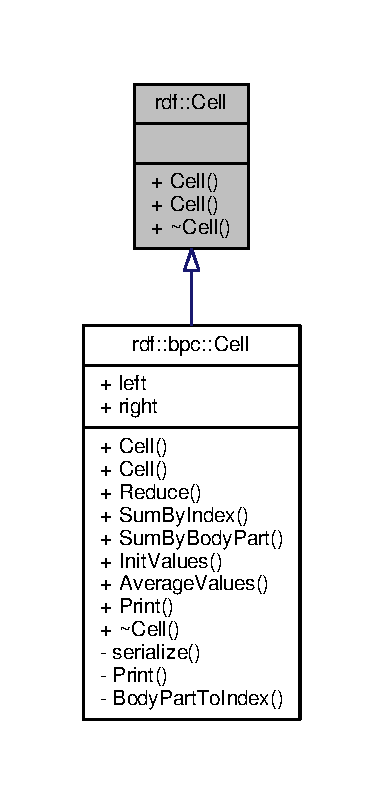
\includegraphics[width=184pt]{classrdf_1_1Cell__inherit__graph}
\end{center}
\end{figure}


Collaboration diagram for rdf\+:\+:Cell\+:
\nopagebreak
\begin{figure}[H]
\begin{center}
\leavevmode
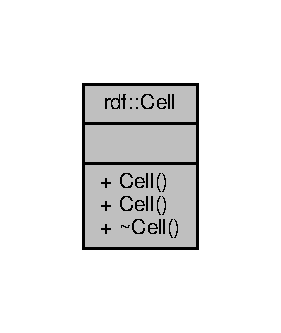
\includegraphics[width=135pt]{classrdf_1_1Cell__coll__graph}
\end{center}
\end{figure}
\subsection*{Public Member Functions}
\begin{DoxyCompactItemize}
\item 
\hyperlink{classrdf_1_1Cell_ae615dc1f204198c07c0c98728e8200d2}{Cell} ()
\item 
\hyperlink{classrdf_1_1Cell_aaf07af9d5638d3b80e6e35286d5b27d9}{Cell} (const \hyperlink{classrdf_1_1Cell}{Cell} \&orig)
\item 
virtual \hyperlink{classrdf_1_1Cell_a25a097dcee67ea115326ec0aaeea8e4a}{$\sim$\+Cell} ()
\end{DoxyCompactItemize}


\subsection{Constructor \& Destructor Documentation}
\index{rdf\+::\+Cell@{rdf\+::\+Cell}!Cell@{Cell}}
\index{Cell@{Cell}!rdf\+::\+Cell@{rdf\+::\+Cell}}
\subsubsection[{\texorpdfstring{Cell()}{Cell()}}]{\setlength{\rightskip}{0pt plus 5cm}rdf\+::\+Cell\+::\+Cell (
\begin{DoxyParamCaption}
{}
\end{DoxyParamCaption}
)}\hypertarget{classrdf_1_1Cell_ae615dc1f204198c07c0c98728e8200d2}{}\label{classrdf_1_1Cell_ae615dc1f204198c07c0c98728e8200d2}

\begin{DoxyCode}
29              \{
30     \textcolor{comment}{//    int nBodyParts = 10;}
31     \textcolor{comment}{//    left.resize(nBodyParts, 0);}
32     \textcolor{comment}{//    right.resize(nBodyParts, 0);}
33   \}
\end{DoxyCode}
\index{rdf\+::\+Cell@{rdf\+::\+Cell}!Cell@{Cell}}
\index{Cell@{Cell}!rdf\+::\+Cell@{rdf\+::\+Cell}}
\subsubsection[{\texorpdfstring{Cell(const Cell \&orig)}{Cell(const Cell &orig)}}]{\setlength{\rightskip}{0pt plus 5cm}rdf\+::\+Cell\+::\+Cell (
\begin{DoxyParamCaption}
\item[{const {\bf Cell} \&}]{orig}
\end{DoxyParamCaption}
)}\hypertarget{classrdf_1_1Cell_aaf07af9d5638d3b80e6e35286d5b27d9}{}\label{classrdf_1_1Cell_aaf07af9d5638d3b80e6e35286d5b27d9}

\begin{DoxyCode}
36                              \{
37   \}
\end{DoxyCode}
\index{rdf\+::\+Cell@{rdf\+::\+Cell}!````~Cell@{$\sim$\+Cell}}
\index{````~Cell@{$\sim$\+Cell}!rdf\+::\+Cell@{rdf\+::\+Cell}}
\subsubsection[{\texorpdfstring{$\sim$\+Cell()}{~Cell()}}]{\setlength{\rightskip}{0pt plus 5cm}rdf\+::\+Cell\+::$\sim$\+Cell (
\begin{DoxyParamCaption}
{}
\end{DoxyParamCaption}
)\hspace{0.3cm}{\ttfamily [virtual]}}\hypertarget{classrdf_1_1Cell_a25a097dcee67ea115326ec0aaeea8e4a}{}\label{classrdf_1_1Cell_a25a097dcee67ea115326ec0aaeea8e4a}


Reimplemented in \hyperlink{classrdf_1_1bpc_1_1Cell_a6e00e0aeaca79249ce8d21bee8ca0b62}{rdf\+::bpc\+::\+Cell}.


\begin{DoxyCode}
40               \{
41   \}
\end{DoxyCode}


The documentation for this class was generated from the following files\+:\begin{DoxyCompactItemize}
\item 
\hyperlink{Cell_8h}{Cell.\+h}\item 
\hyperlink{Cell_8cpp}{Cell.\+cpp}\end{DoxyCompactItemize}

\hypertarget{classrdf_1_1bpc_1_1Cell}{}\section{rdf\+:\+:bpc\+:\+:Cell Class Reference}
\label{classrdf_1_1bpc_1_1Cell}\index{rdf\+::bpc\+::\+Cell@{rdf\+::bpc\+::\+Cell}}


{\ttfamily \#include $<$Cell\+B\+P\+C.\+h$>$}



Inheritance diagram for rdf\+:\+:bpc\+:\+:Cell\+:
\nopagebreak
\begin{figure}[H]
\begin{center}
\leavevmode
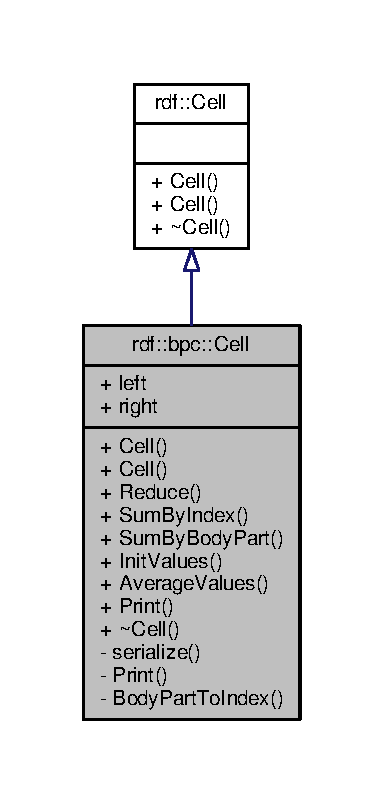
\includegraphics[width=184pt]{classrdf_1_1bpc_1_1Cell__inherit__graph}
\end{center}
\end{figure}


Collaboration diagram for rdf\+:\+:bpc\+:\+:Cell\+:
\nopagebreak
\begin{figure}[H]
\begin{center}
\leavevmode
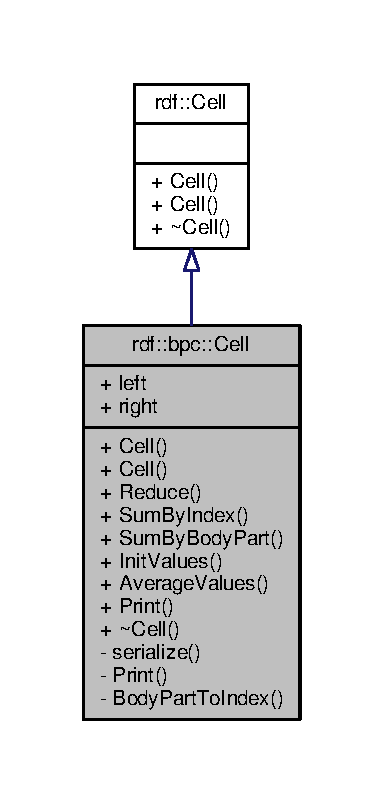
\includegraphics[width=184pt]{classrdf_1_1bpc_1_1Cell__coll__graph}
\end{center}
\end{figure}
\subsection*{Public Member Functions}
\begin{DoxyCompactItemize}
\item 
\hyperlink{classrdf_1_1bpc_1_1Cell_a4e55c973f2869d6145b2e4598f73d915}{Cell} ()
\item 
\hyperlink{classrdf_1_1bpc_1_1Cell_afd3bd26a7eaa27e1842a90ee01560833}{Cell} (const \hyperlink{classrdf_1_1bpc_1_1Cell}{Cell} \&orig)
\item 
void \hyperlink{classrdf_1_1bpc_1_1Cell_a163b21f78c2cd0319926292773b68269}{Reduce} (const \hyperlink{classrdf_1_1bpc_1_1Cell}{Cell} \&other)
\item 
void \hyperlink{classrdf_1_1bpc_1_1Cell_a8867ff9846fcd8e0ae6ca0cd754230d1}{Sum\+By\+Index} (int to\+Left, int index, float val)
\item 
void \hyperlink{classrdf_1_1bpc_1_1Cell_a23a09c0ba4e7b6e52176276d464eb982}{Sum\+By\+Body\+Part} (int to\+Left, std\+::string body\+Part, float val)
\item 
void \hyperlink{classrdf_1_1bpc_1_1Cell_ad4ed0c5ddb5690a2a4ea21bb1d897072}{Init\+Values} (float left\+Vals, float right\+Vals)
\item 
void \hyperlink{classrdf_1_1bpc_1_1Cell_ab493e3da763f35681744705d05518412}{Average\+Values} (int num)
\item 
void \hyperlink{classrdf_1_1bpc_1_1Cell_afbdaa564c364a52d937f4474cb37c99a}{Print} ()
\item 
virtual \hyperlink{classrdf_1_1bpc_1_1Cell_a6e00e0aeaca79249ce8d21bee8ca0b62}{$\sim$\+Cell} ()
\end{DoxyCompactItemize}
\subsection*{Public Attributes}
\begin{DoxyCompactItemize}
\item 
std\+::vector$<$ float $>$ \hyperlink{classrdf_1_1bpc_1_1Cell_acca5eb5901f629ff44710f56934dfba2}{left}
\item 
std\+::vector$<$ float $>$ \hyperlink{classrdf_1_1bpc_1_1Cell_a2d7be4deab042275199ade765509fcea}{right}
\end{DoxyCompactItemize}
\subsection*{Private Member Functions}
\begin{DoxyCompactItemize}
\item 
{\footnotesize template$<$class Archive $>$ }\\void \hyperlink{classrdf_1_1bpc_1_1Cell_a2ff77bef68243ee1b3f87ba3d841a07e}{serialize} (Archive \&ar, const unsigned int version)
\item 
void \hyperlink{classrdf_1_1bpc_1_1Cell_a6263cc208881c9795837fdebf10592e7}{Print} (int i)
\item 
int \hyperlink{classrdf_1_1bpc_1_1Cell_a00bde32e84e23b71d83a6e5e62d45e6d}{Body\+Part\+To\+Index} (std\+::string body\+Part)
\end{DoxyCompactItemize}
\subsection*{Friends}
\begin{DoxyCompactItemize}
\item 
class \hyperlink{classrdf_1_1bpc_1_1Cell_ac98d07dd8f7b70e16ccb9a01abf56b9c}{boost\+::serialization\+::access}
\end{DoxyCompactItemize}


\subsection{Constructor \& Destructor Documentation}
\index{rdf\+::bpc\+::\+Cell@{rdf\+::bpc\+::\+Cell}!Cell@{Cell}}
\index{Cell@{Cell}!rdf\+::bpc\+::\+Cell@{rdf\+::bpc\+::\+Cell}}
\subsubsection[{\texorpdfstring{Cell()}{Cell()}}]{\setlength{\rightskip}{0pt plus 5cm}rdf\+::bpc\+::\+Cell\+::\+Cell (
\begin{DoxyParamCaption}
{}
\end{DoxyParamCaption}
)}\hypertarget{classrdf_1_1bpc_1_1Cell_a4e55c973f2869d6145b2e4598f73d915}{}\label{classrdf_1_1bpc_1_1Cell_a4e55c973f2869d6145b2e4598f73d915}


References B\+O\+D\+Y\+\_\+\+P\+A\+R\+T\+S\+\_\+\+N\+UM, left, and right.


\begin{DoxyCode}
29                \{
30       \hyperlink{classrdf_1_1bpc_1_1Cell_acca5eb5901f629ff44710f56934dfba2}{left}.resize(\hyperlink{CellBPC_8h_ae850b88fe99c39799aca5022cde5f295}{BODY\_PARTS\_NUM}, 8.0);
31       \hyperlink{classrdf_1_1bpc_1_1Cell_a2d7be4deab042275199ade765509fcea}{right}.resize(\hyperlink{CellBPC_8h_ae850b88fe99c39799aca5022cde5f295}{BODY\_PARTS\_NUM}, 1.0);
32     \}
\end{DoxyCode}
\index{rdf\+::bpc\+::\+Cell@{rdf\+::bpc\+::\+Cell}!Cell@{Cell}}
\index{Cell@{Cell}!rdf\+::bpc\+::\+Cell@{rdf\+::bpc\+::\+Cell}}
\subsubsection[{\texorpdfstring{Cell(const Cell \&orig)}{Cell(const Cell &orig)}}]{\setlength{\rightskip}{0pt plus 5cm}rdf\+::bpc\+::\+Cell\+::\+Cell (
\begin{DoxyParamCaption}
\item[{const {\bf Cell} \&}]{orig}
\end{DoxyParamCaption}
)}\hypertarget{classrdf_1_1bpc_1_1Cell_afd3bd26a7eaa27e1842a90ee01560833}{}\label{classrdf_1_1bpc_1_1Cell_afd3bd26a7eaa27e1842a90ee01560833}


References left, and right.


\begin{DoxyCode}
34                                \{
35       \hyperlink{classrdf_1_1bpc_1_1Cell_acca5eb5901f629ff44710f56934dfba2}{left} = orig.left;
36       \hyperlink{classrdf_1_1bpc_1_1Cell_a2d7be4deab042275199ade765509fcea}{right} = orig.right;
37     \}
\end{DoxyCode}
\index{rdf\+::bpc\+::\+Cell@{rdf\+::bpc\+::\+Cell}!````~Cell@{$\sim$\+Cell}}
\index{````~Cell@{$\sim$\+Cell}!rdf\+::bpc\+::\+Cell@{rdf\+::bpc\+::\+Cell}}
\subsubsection[{\texorpdfstring{$\sim$\+Cell()}{~Cell()}}]{\setlength{\rightskip}{0pt plus 5cm}rdf\+::bpc\+::\+Cell\+::$\sim$\+Cell (
\begin{DoxyParamCaption}
{}
\end{DoxyParamCaption}
)\hspace{0.3cm}{\ttfamily [virtual]}}\hypertarget{classrdf_1_1bpc_1_1Cell_a6e00e0aeaca79249ce8d21bee8ca0b62}{}\label{classrdf_1_1bpc_1_1Cell_a6e00e0aeaca79249ce8d21bee8ca0b62}


Reimplemented from \hyperlink{classrdf_1_1Cell_a25a097dcee67ea115326ec0aaeea8e4a}{rdf\+::\+Cell}.


\begin{DoxyCode}
106                 \{
107 
108     \}
\end{DoxyCode}


\subsection{Member Function Documentation}
\index{rdf\+::bpc\+::\+Cell@{rdf\+::bpc\+::\+Cell}!Average\+Values@{Average\+Values}}
\index{Average\+Values@{Average\+Values}!rdf\+::bpc\+::\+Cell@{rdf\+::bpc\+::\+Cell}}
\subsubsection[{\texorpdfstring{Average\+Values(int num)}{AverageValues(int num)}}]{\setlength{\rightskip}{0pt plus 5cm}void rdf\+::bpc\+::\+Cell\+::\+Average\+Values (
\begin{DoxyParamCaption}
\item[{int}]{num}
\end{DoxyParamCaption}
)}\hypertarget{classrdf_1_1bpc_1_1Cell_ab493e3da763f35681744705d05518412}{}\label{classrdf_1_1bpc_1_1Cell_ab493e3da763f35681744705d05518412}


References B\+O\+D\+Y\+\_\+\+P\+A\+R\+T\+S\+\_\+\+N\+UM, left, and right.


\begin{DoxyCode}
67                                    \{
68       \textcolor{keywordflow}{for} (\textcolor{keywordtype}{int} i = 0; i < \hyperlink{CellBPC_8h_ae850b88fe99c39799aca5022cde5f295}{BODY\_PARTS\_NUM}; i++) \{
69         \hyperlink{classrdf_1_1bpc_1_1Cell_acca5eb5901f629ff44710f56934dfba2}{left}[i] = \hyperlink{classrdf_1_1bpc_1_1Cell_acca5eb5901f629ff44710f56934dfba2}{left}[i] / num;
70         \hyperlink{classrdf_1_1bpc_1_1Cell_a2d7be4deab042275199ade765509fcea}{right}[i] = \hyperlink{classrdf_1_1bpc_1_1Cell_a2d7be4deab042275199ade765509fcea}{right}[i] / num;
71       \}
72     \}
\end{DoxyCode}
\index{rdf\+::bpc\+::\+Cell@{rdf\+::bpc\+::\+Cell}!Body\+Part\+To\+Index@{Body\+Part\+To\+Index}}
\index{Body\+Part\+To\+Index@{Body\+Part\+To\+Index}!rdf\+::bpc\+::\+Cell@{rdf\+::bpc\+::\+Cell}}
\subsubsection[{\texorpdfstring{Body\+Part\+To\+Index(std\+::string body\+Part)}{BodyPartToIndex(std::string bodyPart)}}]{\setlength{\rightskip}{0pt plus 5cm}int rdf\+::bpc\+::\+Cell\+::\+Body\+Part\+To\+Index (
\begin{DoxyParamCaption}
\item[{std\+::string}]{body\+Part}
\end{DoxyParamCaption}
)\hspace{0.3cm}{\ttfamily [private]}}\hypertarget{classrdf_1_1bpc_1_1Cell_a00bde32e84e23b71d83a6e5e62d45e6d}{}\label{classrdf_1_1bpc_1_1Cell_a00bde32e84e23b71d83a6e5e62d45e6d}


Referenced by serialize(), and Sum\+By\+Body\+Part().


\begin{DoxyCode}
75                                                \{
76       \textcolor{keywordflow}{if} (bodyPart == \textcolor{stringliteral}{"brazo"})\{
77         \textcolor{keywordflow}{return} 0;
78       \}
79       \textcolor{keywordflow}{else} \textcolor{keywordflow}{if} (bodyPart == \textcolor{stringliteral}{"dedo"})\{
80         \textcolor{keywordflow}{return} 1;
81       \}
82       \textcolor{keywordflow}{else} \textcolor{keywordflow}{if} (bodyPart == \textcolor{stringliteral}{"mano"})\{
83         \textcolor{keywordflow}{return} 2;
84       \}
85       \textcolor{keywordflow}{else} \textcolor{keywordflow}{if} (bodyPart == \textcolor{stringliteral}{"cabeza"})\{
86         \textcolor{keywordflow}{return} 3;
87       \}
88       \textcolor{keywordflow}{else} \textcolor{keywordflow}{if} (bodyPart == \textcolor{stringliteral}{"pecho"})\{
89         \textcolor{keywordflow}{return} 4;
90       \}
91 
92       \textcolor{comment}{/* etc..... */}
93     \}
\end{DoxyCode}
\index{rdf\+::bpc\+::\+Cell@{rdf\+::bpc\+::\+Cell}!Init\+Values@{Init\+Values}}
\index{Init\+Values@{Init\+Values}!rdf\+::bpc\+::\+Cell@{rdf\+::bpc\+::\+Cell}}
\subsubsection[{\texorpdfstring{Init\+Values(float left\+Vals, float right\+Vals)}{InitValues(float leftVals, float rightVals)}}]{\setlength{\rightskip}{0pt plus 5cm}void rdf\+::bpc\+::\+Cell\+::\+Init\+Values (
\begin{DoxyParamCaption}
\item[{float}]{left\+Vals, }
\item[{float}]{right\+Vals}
\end{DoxyParamCaption}
)}\hypertarget{classrdf_1_1bpc_1_1Cell_ad4ed0c5ddb5690a2a4ea21bb1d897072}{}\label{classrdf_1_1bpc_1_1Cell_ad4ed0c5ddb5690a2a4ea21bb1d897072}


References B\+O\+D\+Y\+\_\+\+P\+A\+R\+T\+S\+\_\+\+N\+UM, left, and right.


\begin{DoxyCode}
50                                                             \{
51       \textcolor{keywordflow}{for} (\textcolor{keywordtype}{int} i = 0; i < \hyperlink{CellBPC_8h_ae850b88fe99c39799aca5022cde5f295}{BODY\_PARTS\_NUM}; i++) \{
52         \hyperlink{classrdf_1_1bpc_1_1Cell_acca5eb5901f629ff44710f56934dfba2}{left}[i] = leftValues;
53         \hyperlink{classrdf_1_1bpc_1_1Cell_a2d7be4deab042275199ade765509fcea}{right}[i] = rightValues;
54       \}
55     \}
\end{DoxyCode}
\index{rdf\+::bpc\+::\+Cell@{rdf\+::bpc\+::\+Cell}!Print@{Print}}
\index{Print@{Print}!rdf\+::bpc\+::\+Cell@{rdf\+::bpc\+::\+Cell}}
\subsubsection[{\texorpdfstring{Print()}{Print()}}]{\setlength{\rightskip}{0pt plus 5cm}void rdf\+::bpc\+::\+Cell\+::\+Print (
\begin{DoxyParamCaption}
{}
\end{DoxyParamCaption}
)}\hypertarget{classrdf_1_1bpc_1_1Cell_afbdaa564c364a52d937f4474cb37c99a}{}\label{classrdf_1_1bpc_1_1Cell_afbdaa564c364a52d937f4474cb37c99a}


References B\+O\+D\+Y\+\_\+\+P\+A\+R\+T\+S\+\_\+\+N\+UM, left, and right.



Referenced by serialize().


\begin{DoxyCode}
96                     \{
97       \textcolor{keywordflow}{for} (\textcolor{keywordtype}{int} i = 0; i < \hyperlink{CellBPC_8h_ae850b88fe99c39799aca5022cde5f295}{BODY\_PARTS\_NUM}; i++) \{
98         std::cout << \textcolor{stringliteral}{"Left: "} << \hyperlink{classrdf_1_1bpc_1_1Cell_acca5eb5901f629ff44710f56934dfba2}{left}[i] << \textcolor{stringliteral}{"\(\backslash\)tRight: "} << \hyperlink{classrdf_1_1bpc_1_1Cell_a2d7be4deab042275199ade765509fcea}{right}[i] << std::endl;
99       \}
100     \}
\end{DoxyCode}
\index{rdf\+::bpc\+::\+Cell@{rdf\+::bpc\+::\+Cell}!Print@{Print}}
\index{Print@{Print}!rdf\+::bpc\+::\+Cell@{rdf\+::bpc\+::\+Cell}}
\subsubsection[{\texorpdfstring{Print(int i)}{Print(int i)}}]{\setlength{\rightskip}{0pt plus 5cm}void rdf\+::bpc\+::\+Cell\+::\+Print (
\begin{DoxyParamCaption}
\item[{int}]{i}
\end{DoxyParamCaption}
)\hspace{0.3cm}{\ttfamily [private]}}\hypertarget{classrdf_1_1bpc_1_1Cell_a6263cc208881c9795837fdebf10592e7}{}\label{classrdf_1_1bpc_1_1Cell_a6263cc208881c9795837fdebf10592e7}


References left, and right.


\begin{DoxyCode}
102                          \{
103         std::cout << \textcolor{stringliteral}{"i["} << i << \textcolor{stringliteral}{"]"} <<\textcolor{stringliteral}{"Left: "} << \hyperlink{classrdf_1_1bpc_1_1Cell_acca5eb5901f629ff44710f56934dfba2}{left}[i] << \textcolor{stringliteral}{"\(\backslash\)tRight: "} << 
      \hyperlink{classrdf_1_1bpc_1_1Cell_a2d7be4deab042275199ade765509fcea}{right}[i] << std::endl;
104     \}
\end{DoxyCode}
\index{rdf\+::bpc\+::\+Cell@{rdf\+::bpc\+::\+Cell}!Reduce@{Reduce}}
\index{Reduce@{Reduce}!rdf\+::bpc\+::\+Cell@{rdf\+::bpc\+::\+Cell}}
\subsubsection[{\texorpdfstring{Reduce(const Cell \&other)}{Reduce(const Cell &other)}}]{\setlength{\rightskip}{0pt plus 5cm}void rdf\+::bpc\+::\+Cell\+::\+Reduce (
\begin{DoxyParamCaption}
\item[{const {\bf Cell} \&}]{other}
\end{DoxyParamCaption}
)}\hypertarget{classrdf_1_1bpc_1_1Cell_a163b21f78c2cd0319926292773b68269}{}\label{classrdf_1_1bpc_1_1Cell_a163b21f78c2cd0319926292773b68269}


References B\+O\+D\+Y\+\_\+\+P\+A\+R\+T\+S\+\_\+\+N\+UM, left, and right.


\begin{DoxyCode}
39                                        \{
40       \textcolor{keywordtype}{float} otherLeft, otherRight;
41       \textcolor{keywordflow}{for} (\textcolor{keywordtype}{int} i = 0; i < \hyperlink{CellBPC_8h_ae850b88fe99c39799aca5022cde5f295}{BODY\_PARTS\_NUM}; i++) \{
42         otherLeft = other.left[i];
43         otherRight = other.right[i];
44         \hyperlink{classrdf_1_1bpc_1_1Cell_acca5eb5901f629ff44710f56934dfba2}{left}[i] = \hyperlink{classrdf_1_1bpc_1_1Cell_acca5eb5901f629ff44710f56934dfba2}{left}[i] + otherLeft;
45         \hyperlink{classrdf_1_1bpc_1_1Cell_a2d7be4deab042275199ade765509fcea}{right}[i] = \hyperlink{classrdf_1_1bpc_1_1Cell_a2d7be4deab042275199ade765509fcea}{right}[i] + otherRight;
46       \}
47       \textcolor{comment}{// return *this;}
48     \}
\end{DoxyCode}
\index{rdf\+::bpc\+::\+Cell@{rdf\+::bpc\+::\+Cell}!serialize@{serialize}}
\index{serialize@{serialize}!rdf\+::bpc\+::\+Cell@{rdf\+::bpc\+::\+Cell}}
\subsubsection[{\texorpdfstring{serialize(\+Archive \&ar, const unsigned int version)}{serialize(Archive &ar, const unsigned int version)}}]{\setlength{\rightskip}{0pt plus 5cm}template$<$class Archive $>$ void rdf\+::bpc\+::\+Cell\+::serialize (
\begin{DoxyParamCaption}
\item[{Archive \&}]{ar, }
\item[{const unsigned int}]{version}
\end{DoxyParamCaption}
)\hspace{0.3cm}{\ttfamily [inline]}, {\ttfamily [private]}}\hypertarget{classrdf_1_1bpc_1_1Cell_a2ff77bef68243ee1b3f87ba3d841a07e}{}\label{classrdf_1_1bpc_1_1Cell_a2ff77bef68243ee1b3f87ba3d841a07e}


References Body\+Part\+To\+Index(), left, Print(), and right.


\begin{DoxyCode}
67           \{
68             ar & \hyperlink{classrdf_1_1bpc_1_1Cell_acca5eb5901f629ff44710f56934dfba2}{left};
69             ar & \hyperlink{classrdf_1_1bpc_1_1Cell_a2d7be4deab042275199ade765509fcea}{right};
70           \}
\end{DoxyCode}
\index{rdf\+::bpc\+::\+Cell@{rdf\+::bpc\+::\+Cell}!Sum\+By\+Body\+Part@{Sum\+By\+Body\+Part}}
\index{Sum\+By\+Body\+Part@{Sum\+By\+Body\+Part}!rdf\+::bpc\+::\+Cell@{rdf\+::bpc\+::\+Cell}}
\subsubsection[{\texorpdfstring{Sum\+By\+Body\+Part(int to\+Left, std\+::string body\+Part, float val)}{SumByBodyPart(int toLeft, std::string bodyPart, float val)}}]{\setlength{\rightskip}{0pt plus 5cm}void rdf\+::bpc\+::\+Cell\+::\+Sum\+By\+Body\+Part (
\begin{DoxyParamCaption}
\item[{int}]{to\+Left, }
\item[{std\+::string}]{body\+Part, }
\item[{float}]{val}
\end{DoxyParamCaption}
)}\hypertarget{classrdf_1_1bpc_1_1Cell_a23a09c0ba4e7b6e52176276d464eb982}{}\label{classrdf_1_1bpc_1_1Cell_a23a09c0ba4e7b6e52176276d464eb982}


References Body\+Part\+To\+Index(), and Sum\+By\+Index().


\begin{DoxyCode}
61                                                                      \{
62       \textcolor{keywordtype}{int} index = \hyperlink{classrdf_1_1bpc_1_1Cell_a00bde32e84e23b71d83a6e5e62d45e6d}{BodyPartToIndex}(bodyPart);
63       \hyperlink{classrdf_1_1bpc_1_1Cell_a8867ff9846fcd8e0ae6ca0cd754230d1}{SumByIndex}(toLeft, index, val);
64 
65     \}
\end{DoxyCode}
\index{rdf\+::bpc\+::\+Cell@{rdf\+::bpc\+::\+Cell}!Sum\+By\+Index@{Sum\+By\+Index}}
\index{Sum\+By\+Index@{Sum\+By\+Index}!rdf\+::bpc\+::\+Cell@{rdf\+::bpc\+::\+Cell}}
\subsubsection[{\texorpdfstring{Sum\+By\+Index(int to\+Left, int index, float val)}{SumByIndex(int toLeft, int index, float val)}}]{\setlength{\rightskip}{0pt plus 5cm}void rdf\+::bpc\+::\+Cell\+::\+Sum\+By\+Index (
\begin{DoxyParamCaption}
\item[{int}]{to\+Left, }
\item[{int}]{index, }
\item[{float}]{val}
\end{DoxyParamCaption}
)}\hypertarget{classrdf_1_1bpc_1_1Cell_a8867ff9846fcd8e0ae6ca0cd754230d1}{}\label{classrdf_1_1bpc_1_1Cell_a8867ff9846fcd8e0ae6ca0cd754230d1}


References left, and right.



Referenced by Sum\+By\+Body\+Part().


\begin{DoxyCode}
57                                                            \{
58       (toLeft) ? \hyperlink{classrdf_1_1bpc_1_1Cell_acca5eb5901f629ff44710f56934dfba2}{left}[index] += value : \hyperlink{classrdf_1_1bpc_1_1Cell_a2d7be4deab042275199ade765509fcea}{right}[index] += value;
59     \}
\end{DoxyCode}


\subsection{Friends And Related Function Documentation}
\index{rdf\+::bpc\+::\+Cell@{rdf\+::bpc\+::\+Cell}!boost\+::serialization\+::access@{boost\+::serialization\+::access}}
\index{boost\+::serialization\+::access@{boost\+::serialization\+::access}!rdf\+::bpc\+::\+Cell@{rdf\+::bpc\+::\+Cell}}
\subsubsection[{\texorpdfstring{boost\+::serialization\+::access}{boost::serialization::access}}]{\setlength{\rightskip}{0pt plus 5cm}friend class boost\+::serialization\+::access\hspace{0.3cm}{\ttfamily [friend]}}\hypertarget{classrdf_1_1bpc_1_1Cell_ac98d07dd8f7b70e16ccb9a01abf56b9c}{}\label{classrdf_1_1bpc_1_1Cell_ac98d07dd8f7b70e16ccb9a01abf56b9c}


\subsection{Member Data Documentation}
\index{rdf\+::bpc\+::\+Cell@{rdf\+::bpc\+::\+Cell}!left@{left}}
\index{left@{left}!rdf\+::bpc\+::\+Cell@{rdf\+::bpc\+::\+Cell}}
\subsubsection[{\texorpdfstring{left}{left}}]{\setlength{\rightskip}{0pt plus 5cm}std\+::vector$<$float$>$ rdf\+::bpc\+::\+Cell\+::left}\hypertarget{classrdf_1_1bpc_1_1Cell_acca5eb5901f629ff44710f56934dfba2}{}\label{classrdf_1_1bpc_1_1Cell_acca5eb5901f629ff44710f56934dfba2}


Referenced by Average\+Values(), Cell(), Init\+Values(), Print(), Reduce(), serialize(), and Sum\+By\+Index().

\index{rdf\+::bpc\+::\+Cell@{rdf\+::bpc\+::\+Cell}!right@{right}}
\index{right@{right}!rdf\+::bpc\+::\+Cell@{rdf\+::bpc\+::\+Cell}}
\subsubsection[{\texorpdfstring{right}{right}}]{\setlength{\rightskip}{0pt plus 5cm}std\+::vector$<$float$>$ rdf\+::bpc\+::\+Cell\+::right}\hypertarget{classrdf_1_1bpc_1_1Cell_a2d7be4deab042275199ade765509fcea}{}\label{classrdf_1_1bpc_1_1Cell_a2d7be4deab042275199ade765509fcea}


Referenced by Average\+Values(), Cell(), Init\+Values(), Print(), Reduce(), serialize(), and Sum\+By\+Index().



The documentation for this class was generated from the following files\+:\begin{DoxyCompactItemize}
\item 
\hyperlink{CellBPC_8h}{Cell\+B\+P\+C.\+h}\item 
\hyperlink{CellBPC_8cpp}{Cell\+B\+P\+C.\+cpp}\end{DoxyCompactItemize}

\hypertarget{classCollection}{}\section{Collection Class Reference}
\label{classCollection}\index{Collection@{Collection}}


{\ttfamily \#include $<$Collection.\+h$>$}



Collaboration diagram for Collection\+:
\nopagebreak
\begin{figure}[H]
\begin{center}
\leavevmode
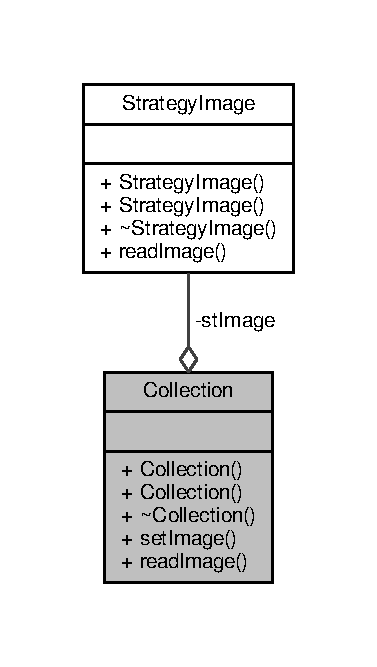
\includegraphics[width=181pt]{classCollection__coll__graph}
\end{center}
\end{figure}
\subsection*{Public Member Functions}
\begin{DoxyCompactItemize}
\item 
\hyperlink{classCollection_a1fda66d6a2ff4fcecc74fba63abbf52f}{Collection} ()
\item 
\hyperlink{classCollection_ab42c1cfe26f486bd060cbbe215c374f0}{Collection} (const \hyperlink{classCollection}{Collection} \&orig)
\item 
virtual \hyperlink{classCollection_a017dd492156e6b570a21f58a07dd73f5}{$\sim$\+Collection} ()
\item 
void \hyperlink{classCollection_a57290652c3cf6fc744c5614e0bf49d15}{set\+Image} (\hyperlink{classStrategyImage}{Strategy\+Image} $\ast$Type\+Image)
\item 
void \hyperlink{classCollection_a251f7033e22c16a7b12dde94d9a7021e}{read\+Image} (int height, int width, std\+::string direction, cv\+::\+Mat \&image)
\end{DoxyCompactItemize}
\subsection*{Private Attributes}
\begin{DoxyCompactItemize}
\item 
\hyperlink{classStrategyImage}{Strategy\+Image} $\ast$ \hyperlink{classCollection_a0831c53adfb080139a54b8c7a98bdf25}{st\+Image}
\end{DoxyCompactItemize}


\subsection{Constructor \& Destructor Documentation}
\index{Collection@{Collection}!Collection@{Collection}}
\index{Collection@{Collection}!Collection@{Collection}}
\subsubsection[{\texorpdfstring{Collection()}{Collection()}}]{\setlength{\rightskip}{0pt plus 5cm}Collection\+::\+Collection (
\begin{DoxyParamCaption}
{}
\end{DoxyParamCaption}
)}\hypertarget{classCollection_a1fda66d6a2ff4fcecc74fba63abbf52f}{}\label{classCollection_a1fda66d6a2ff4fcecc74fba63abbf52f}

\begin{DoxyCode}
16                        \{
17 \}
\end{DoxyCode}
\index{Collection@{Collection}!Collection@{Collection}}
\index{Collection@{Collection}!Collection@{Collection}}
\subsubsection[{\texorpdfstring{Collection(const Collection \&orig)}{Collection(const Collection &orig)}}]{\setlength{\rightskip}{0pt plus 5cm}Collection\+::\+Collection (
\begin{DoxyParamCaption}
\item[{const {\bf Collection} \&}]{orig}
\end{DoxyParamCaption}
)}\hypertarget{classCollection_ab42c1cfe26f486bd060cbbe215c374f0}{}\label{classCollection_ab42c1cfe26f486bd060cbbe215c374f0}

\begin{DoxyCode}
19                                              \{
20 \}
\end{DoxyCode}
\index{Collection@{Collection}!````~Collection@{$\sim$\+Collection}}
\index{````~Collection@{$\sim$\+Collection}!Collection@{Collection}}
\subsubsection[{\texorpdfstring{$\sim$\+Collection()}{~Collection()}}]{\setlength{\rightskip}{0pt plus 5cm}Collection\+::$\sim$\+Collection (
\begin{DoxyParamCaption}
{}
\end{DoxyParamCaption}
)\hspace{0.3cm}{\ttfamily [virtual]}}\hypertarget{classCollection_a017dd492156e6b570a21f58a07dd73f5}{}\label{classCollection_a017dd492156e6b570a21f58a07dd73f5}

\begin{DoxyCode}
22                         \{
23 \}
\end{DoxyCode}


\subsection{Member Function Documentation}
\index{Collection@{Collection}!read\+Image@{read\+Image}}
\index{read\+Image@{read\+Image}!Collection@{Collection}}
\subsubsection[{\texorpdfstring{read\+Image(int height, int width, std\+::string direction, cv\+::\+Mat \&image)}{readImage(int height, int width, std::string direction, cv::Mat &image)}}]{\setlength{\rightskip}{0pt plus 5cm}void Collection\+::read\+Image (
\begin{DoxyParamCaption}
\item[{int}]{height, }
\item[{int}]{width, }
\item[{std\+::string}]{direction, }
\item[{cv\+::\+Mat \&}]{image}
\end{DoxyParamCaption}
)}\hypertarget{classCollection_a251f7033e22c16a7b12dde94d9a7021e}{}\label{classCollection_a251f7033e22c16a7b12dde94d9a7021e}


References Strategy\+Image\+::read\+Image(), and st\+Image.



Referenced by Image\+::generated\+Structure\+Shotton().


\begin{DoxyCode}
30                                                                                   \{
31     cv::Mat imageTem;
32     \hyperlink{classCollection_a0831c53adfb080139a54b8c7a98bdf25}{Collection::stImage}->\hyperlink{classStrategyImage_aee857e79df483412f66b529417ddfd44}{readImage}(height,width,direction,imageTem);
33     image = imageTem;
34     
35 \}\end{DoxyCode}
\index{Collection@{Collection}!set\+Image@{set\+Image}}
\index{set\+Image@{set\+Image}!Collection@{Collection}}
\subsubsection[{\texorpdfstring{set\+Image(\+Strategy\+Image $\ast$\+Type\+Image)}{setImage(StrategyImage *TypeImage)}}]{\setlength{\rightskip}{0pt plus 5cm}void Collection\+::set\+Image (
\begin{DoxyParamCaption}
\item[{{\bf Strategy\+Image} $\ast$}]{Type\+Image}
\end{DoxyParamCaption}
)}\hypertarget{classCollection_a57290652c3cf6fc744c5614e0bf49d15}{}\label{classCollection_a57290652c3cf6fc744c5614e0bf49d15}


References st\+Image.



Referenced by Image\+::generated\+Structure\+Shotton().


\begin{DoxyCode}
26                                                  \{
27     \hyperlink{classCollection_a0831c53adfb080139a54b8c7a98bdf25}{Collection::stImage} = TypeImage;
28 \}
\end{DoxyCode}


\subsection{Member Data Documentation}
\index{Collection@{Collection}!st\+Image@{st\+Image}}
\index{st\+Image@{st\+Image}!Collection@{Collection}}
\subsubsection[{\texorpdfstring{st\+Image}{stImage}}]{\setlength{\rightskip}{0pt plus 5cm}{\bf Strategy\+Image}$\ast$ Collection\+::st\+Image\hspace{0.3cm}{\ttfamily [private]}}\hypertarget{classCollection_a0831c53adfb080139a54b8c7a98bdf25}{}\label{classCollection_a0831c53adfb080139a54b8c7a98bdf25}


Referenced by read\+Image(), and set\+Image().



The documentation for this class was generated from the following files\+:\begin{DoxyCompactItemize}
\item 
\hyperlink{Collection_8h}{Collection.\+h}\item 
\hyperlink{Collection_8cpp}{Collection.\+cpp}\end{DoxyCompactItemize}

\hypertarget{classConfigData}{}\section{Config\+Data Class Reference}
\label{classConfigData}\index{Config\+Data@{Config\+Data}}


{\ttfamily \#include $<$Config\+Data.\+h$>$}



Collaboration diagram for Config\+Data\+:
\nopagebreak
\begin{figure}[H]
\begin{center}
\leavevmode
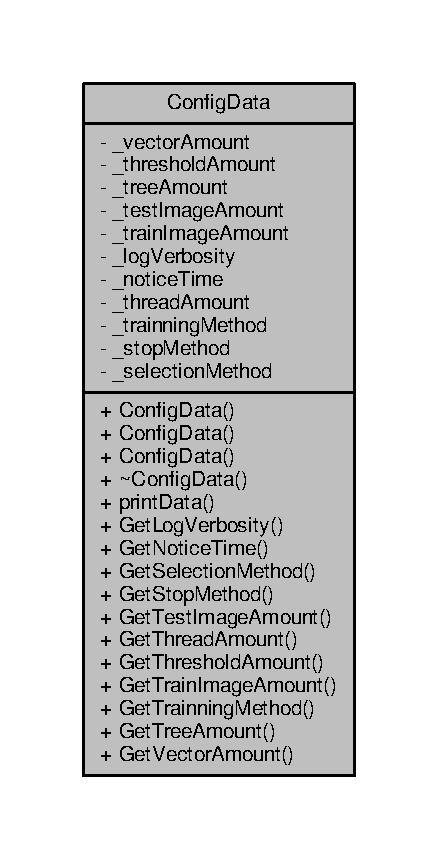
\includegraphics[width=210pt]{classConfigData__coll__graph}
\end{center}
\end{figure}
\subsection*{Public Member Functions}
\begin{DoxyCompactItemize}
\item 
\hyperlink{classConfigData_adb78a42cc714fe0bfdf03d9a1e3d0cc5}{Config\+Data} ()
\item 
\hyperlink{classConfigData_afee1cf6f73db7bc62401d1ac89011fc7}{Config\+Data} (const \hyperlink{classConfigData}{Config\+Data} \&orig)
\item 
\hyperlink{classConfigData_aef5ec959c1c6db9d3be62794f6d61f21}{Config\+Data} (const int \hyperlink{classConfigData_af590033be1d5469272aa1010353232d5}{\+\_\+vector\+Amount}, const int \hyperlink{classConfigData_a1956520556b7b407196a5b4153f6b083}{\+\_\+threshold\+Amount}, const int \hyperlink{classConfigData_a4a8f85fa6d12865575b2226939964a09}{\+\_\+tree\+Amount}, const int \hyperlink{classConfigData_a40355707f3b365a9b83b7530e0de1316}{\+\_\+test\+Image\+Amount}, const int \hyperlink{classConfigData_aa9ece3a15e191b330db21d48b4f092e2}{\+\_\+train\+Image\+Amount}, const int \hyperlink{classConfigData_aa8483944273e9eaa13dff184a8079633}{\+\_\+log\+Verbosity}, const int \hyperlink{classConfigData_a1b82ac5b308abfd0e5a8e4eccec72076}{\+\_\+notice\+Time}, const int \hyperlink{classConfigData_a349c395a667ed45ff0fc4bd0753e890b}{\+\_\+thread\+Amount}, const int \hyperlink{classConfigData_a161bf96e6b8d33d2bf10b86f82546b36}{\+\_\+trainning\+Method}, const int \hyperlink{classConfigData_a0f6db7bbe04644529713729e929b67c0}{\+\_\+stop\+Method}, const int \hyperlink{classConfigData_a348ab0349d09526606e839a639881172}{\+\_\+selection\+Method})
\item 
virtual \hyperlink{classConfigData_a08a1687a8edc7ef9b9db7bd504f8364b}{$\sim$\+Config\+Data} ()
\item 
void \hyperlink{classConfigData_acf8c34f47f52ee33edbb758f795ba5a3}{print\+Data} ()
\item 
const int \hyperlink{classConfigData_af831aa5589131d606b7c4291d61848e9}{Get\+Log\+Verbosity} () const 
\item 
const int \hyperlink{classConfigData_a0d8da6611acebe44717122fa888ddd84}{Get\+Notice\+Time} () const 
\item 
const int \hyperlink{classConfigData_a126b8dd8e7ebe11d84bc191e8cfe9872}{Get\+Selection\+Method} () const 
\item 
const int \hyperlink{classConfigData_a19eafd8866f32eb7988b2c26ae07302a}{Get\+Stop\+Method} () const 
\item 
const int \hyperlink{classConfigData_a755f73287c31ab6ad686547c0f67641a}{Get\+Test\+Image\+Amount} () const 
\item 
const int \hyperlink{classConfigData_a72073a22e8dd10a9c354e8821d25abd4}{Get\+Thread\+Amount} () const 
\item 
const int \hyperlink{classConfigData_a1a0ff65311568910ec2c6145a8faf87b}{Get\+Threshold\+Amount} () const 
\item 
const int \hyperlink{classConfigData_a1532f5d948132842e62a59eec102b39d}{Get\+Train\+Image\+Amount} () const 
\item 
const int \hyperlink{classConfigData_a41a99ccfad14823c0e269c5a77573ddb}{Get\+Trainning\+Method} () const 
\item 
const int \hyperlink{classConfigData_aeca2d4ca7e24db214de7f7d696ac6658}{Get\+Tree\+Amount} () const 
\item 
const int \hyperlink{classConfigData_aa72a285feefdc4fb2706b84c98e98578}{Get\+Vector\+Amount} () const 
\end{DoxyCompactItemize}
\subsection*{Private Attributes}
\begin{DoxyCompactItemize}
\item 
const int \hyperlink{classConfigData_af590033be1d5469272aa1010353232d5}{\+\_\+vector\+Amount} = 0
\item 
const int \hyperlink{classConfigData_a1956520556b7b407196a5b4153f6b083}{\+\_\+threshold\+Amount} = 0
\item 
const int \hyperlink{classConfigData_a4a8f85fa6d12865575b2226939964a09}{\+\_\+tree\+Amount} = 0
\item 
const int \hyperlink{classConfigData_a40355707f3b365a9b83b7530e0de1316}{\+\_\+test\+Image\+Amount} = 0
\item 
const int \hyperlink{classConfigData_aa9ece3a15e191b330db21d48b4f092e2}{\+\_\+train\+Image\+Amount} = 0
\item 
const int \hyperlink{classConfigData_aa8483944273e9eaa13dff184a8079633}{\+\_\+log\+Verbosity} = 0
\item 
const int \hyperlink{classConfigData_a1b82ac5b308abfd0e5a8e4eccec72076}{\+\_\+notice\+Time} = 0
\item 
const int \hyperlink{classConfigData_a349c395a667ed45ff0fc4bd0753e890b}{\+\_\+thread\+Amount} = 0
\item 
const int \hyperlink{classConfigData_a161bf96e6b8d33d2bf10b86f82546b36}{\+\_\+trainning\+Method} = 0
\item 
const int \hyperlink{classConfigData_a0f6db7bbe04644529713729e929b67c0}{\+\_\+stop\+Method} = 0
\item 
const int \hyperlink{classConfigData_a348ab0349d09526606e839a639881172}{\+\_\+selection\+Method} = 0
\end{DoxyCompactItemize}


\subsection{Constructor \& Destructor Documentation}
\index{Config\+Data@{Config\+Data}!Config\+Data@{Config\+Data}}
\index{Config\+Data@{Config\+Data}!Config\+Data@{Config\+Data}}
\subsubsection[{\texorpdfstring{Config\+Data()}{ConfigData()}}]{\setlength{\rightskip}{0pt plus 5cm}Config\+Data\+::\+Config\+Data (
\begin{DoxyParamCaption}
{}
\end{DoxyParamCaption}
)}\hypertarget{classConfigData_adb78a42cc714fe0bfdf03d9a1e3d0cc5}{}\label{classConfigData_adb78a42cc714fe0bfdf03d9a1e3d0cc5}

\begin{DoxyCode}
16                        \{
17 \}
\end{DoxyCode}
\index{Config\+Data@{Config\+Data}!Config\+Data@{Config\+Data}}
\index{Config\+Data@{Config\+Data}!Config\+Data@{Config\+Data}}
\subsubsection[{\texorpdfstring{Config\+Data(const Config\+Data \&orig)}{ConfigData(const ConfigData &orig)}}]{\setlength{\rightskip}{0pt plus 5cm}Config\+Data\+::\+Config\+Data (
\begin{DoxyParamCaption}
\item[{const {\bf Config\+Data} \&}]{orig}
\end{DoxyParamCaption}
)}\hypertarget{classConfigData_afee1cf6f73db7bc62401d1ac89011fc7}{}\label{classConfigData_afee1cf6f73db7bc62401d1ac89011fc7}

\begin{DoxyCode}
19                                              \{
20     \textcolor{comment}{/*\_vectorAmount       = orig.\_vectorAmount;}
21 \textcolor{comment}{        \_thresholdAmount    = orig.\_thresholdAmount;}
22 \textcolor{comment}{        \_treeAmount         = orig.\_treeAmount;}
23 \textcolor{comment}{        \_testImageAmount    = orig.\_trainImageAmount;}
24 \textcolor{comment}{        \_logVerbosity       = orig.\_logVerbosity;}
25 \textcolor{comment}{        \_noticeTime         = orig.\_noticeTime;}
26 \textcolor{comment}{        \_threadAmount       = orig.\_threadAmount;}
27 \textcolor{comment}{        \_trainImageAmount   = orig.\_trainImageAmount;}
28 \textcolor{comment}{        \_stopMethod         = orig.\_stopMethod;}
29 \textcolor{comment}{        \_selectionMethod    = orig.\_selectionMethod;*/}
30 \}
\end{DoxyCode}
\index{Config\+Data@{Config\+Data}!Config\+Data@{Config\+Data}}
\index{Config\+Data@{Config\+Data}!Config\+Data@{Config\+Data}}
\subsubsection[{\texorpdfstring{Config\+Data(const int \+\_\+vector\+Amount, const int \+\_\+threshold\+Amount, const int \+\_\+tree\+Amount, const int \+\_\+test\+Image\+Amount, const int \+\_\+train\+Image\+Amount, const int \+\_\+log\+Verbosity, const int \+\_\+notice\+Time, const int \+\_\+thread\+Amount, const int \+\_\+trainning\+Method, const int \+\_\+stop\+Method, const int \+\_\+selection\+Method)}{ConfigData(const int _vectorAmount, const int _thresholdAmount, const int _treeAmount, const int _testImageAmount, const int _trainImageAmount, const int _logVerbosity, const int _noticeTime, const int _threadAmount, const int _trainningMethod, const int _stopMethod, const int _selectionMethod)}}]{\setlength{\rightskip}{0pt plus 5cm}Config\+Data\+::\+Config\+Data (
\begin{DoxyParamCaption}
\item[{const int}]{\+\_\+vector\+Amount, }
\item[{const int}]{\+\_\+threshold\+Amount, }
\item[{const int}]{\+\_\+tree\+Amount, }
\item[{const int}]{\+\_\+test\+Image\+Amount, }
\item[{const int}]{\+\_\+train\+Image\+Amount, }
\item[{const int}]{\+\_\+log\+Verbosity, }
\item[{const int}]{\+\_\+notice\+Time, }
\item[{const int}]{\+\_\+thread\+Amount, }
\item[{const int}]{\+\_\+trainning\+Method, }
\item[{const int}]{\+\_\+stop\+Method, }
\item[{const int}]{\+\_\+selection\+Method}
\end{DoxyParamCaption}
)\hspace{0.3cm}{\ttfamily [inline]}}\hypertarget{classConfigData_aef5ec959c1c6db9d3be62794f6d61f21}{}\label{classConfigData_aef5ec959c1c6db9d3be62794f6d61f21}

\begin{DoxyCode}
37                                                                                                            
                                                                                                                  
                                                                                           :
38     \hyperlink{classConfigData_af590033be1d5469272aa1010353232d5}{\_vectorAmount}(\hyperlink{classConfigData_af590033be1d5469272aa1010353232d5}{\_vectorAmount}), \hyperlink{classConfigData_a1956520556b7b407196a5b4153f6b083}{\_thresholdAmount}(
      \hyperlink{classConfigData_a1956520556b7b407196a5b4153f6b083}{\_thresholdAmount}), \hyperlink{classConfigData_a4a8f85fa6d12865575b2226939964a09}{\_treeAmount}(\hyperlink{classConfigData_a4a8f85fa6d12865575b2226939964a09}{\_treeAmount}), 
      \hyperlink{classConfigData_a40355707f3b365a9b83b7530e0de1316}{\_testImageAmount}(\hyperlink{classConfigData_a40355707f3b365a9b83b7530e0de1316}{\_testImageAmount}), 
      \hyperlink{classConfigData_aa9ece3a15e191b330db21d48b4f092e2}{\_trainImageAmount}(\hyperlink{classConfigData_aa9ece3a15e191b330db21d48b4f092e2}{\_trainImageAmount}), 
      \hyperlink{classConfigData_aa8483944273e9eaa13dff184a8079633}{\_logVerbosity}(\hyperlink{classConfigData_aa8483944273e9eaa13dff184a8079633}{\_logVerbosity}), \hyperlink{classConfigData_a1b82ac5b308abfd0e5a8e4eccec72076}{\_noticeTime}(
      \hyperlink{classConfigData_a1b82ac5b308abfd0e5a8e4eccec72076}{\_noticeTime}), \hyperlink{classConfigData_a349c395a667ed45ff0fc4bd0753e890b}{\_threadAmount}(\hyperlink{classConfigData_a349c395a667ed45ff0fc4bd0753e890b}{\_threadAmount}), 
      \hyperlink{classConfigData_a161bf96e6b8d33d2bf10b86f82546b36}{\_trainningMethod}(\hyperlink{classConfigData_a161bf96e6b8d33d2bf10b86f82546b36}{\_trainningMethod}), \hyperlink{classConfigData_a0f6db7bbe04644529713729e929b67c0}{\_stopMethod}(
      \hyperlink{classConfigData_a0f6db7bbe04644529713729e929b67c0}{\_stopMethod}), \hyperlink{classConfigData_a348ab0349d09526606e839a639881172}{\_selectionMethod}(\hyperlink{classConfigData_a348ab0349d09526606e839a639881172}{\_selectionMethod}) \{
39     \}
\end{DoxyCode}
\index{Config\+Data@{Config\+Data}!````~Config\+Data@{$\sim$\+Config\+Data}}
\index{````~Config\+Data@{$\sim$\+Config\+Data}!Config\+Data@{Config\+Data}}
\subsubsection[{\texorpdfstring{$\sim$\+Config\+Data()}{~ConfigData()}}]{\setlength{\rightskip}{0pt plus 5cm}Config\+Data\+::$\sim$\+Config\+Data (
\begin{DoxyParamCaption}
{}
\end{DoxyParamCaption}
)\hspace{0.3cm}{\ttfamily [virtual]}}\hypertarget{classConfigData_a08a1687a8edc7ef9b9db7bd504f8364b}{}\label{classConfigData_a08a1687a8edc7ef9b9db7bd504f8364b}

\begin{DoxyCode}
32                         \{
33 \}
\end{DoxyCode}


\subsection{Member Function Documentation}
\index{Config\+Data@{Config\+Data}!Get\+Log\+Verbosity@{Get\+Log\+Verbosity}}
\index{Get\+Log\+Verbosity@{Get\+Log\+Verbosity}!Config\+Data@{Config\+Data}}
\subsubsection[{\texorpdfstring{Get\+Log\+Verbosity() const }{GetLogVerbosity() const }}]{\setlength{\rightskip}{0pt plus 5cm}const int Config\+Data\+::\+Get\+Log\+Verbosity (
\begin{DoxyParamCaption}
{}
\end{DoxyParamCaption}
) const\hspace{0.3cm}{\ttfamily [inline]}}\hypertarget{classConfigData_af831aa5589131d606b7c4291d61848e9}{}\label{classConfigData_af831aa5589131d606b7c4291d61848e9}

\begin{DoxyCode}
44                                       \{
45         \textcolor{keywordflow}{return} \hyperlink{classConfigData_aa8483944273e9eaa13dff184a8079633}{\_logVerbosity};
46     \}
\end{DoxyCode}
\index{Config\+Data@{Config\+Data}!Get\+Notice\+Time@{Get\+Notice\+Time}}
\index{Get\+Notice\+Time@{Get\+Notice\+Time}!Config\+Data@{Config\+Data}}
\subsubsection[{\texorpdfstring{Get\+Notice\+Time() const }{GetNoticeTime() const }}]{\setlength{\rightskip}{0pt plus 5cm}const int Config\+Data\+::\+Get\+Notice\+Time (
\begin{DoxyParamCaption}
{}
\end{DoxyParamCaption}
) const\hspace{0.3cm}{\ttfamily [inline]}}\hypertarget{classConfigData_a0d8da6611acebe44717122fa888ddd84}{}\label{classConfigData_a0d8da6611acebe44717122fa888ddd84}

\begin{DoxyCode}
48                                     \{
49         \textcolor{keywordflow}{return} \hyperlink{classConfigData_a1b82ac5b308abfd0e5a8e4eccec72076}{\_noticeTime};
50     \}
\end{DoxyCode}
\index{Config\+Data@{Config\+Data}!Get\+Selection\+Method@{Get\+Selection\+Method}}
\index{Get\+Selection\+Method@{Get\+Selection\+Method}!Config\+Data@{Config\+Data}}
\subsubsection[{\texorpdfstring{Get\+Selection\+Method() const }{GetSelectionMethod() const }}]{\setlength{\rightskip}{0pt plus 5cm}const int Config\+Data\+::\+Get\+Selection\+Method (
\begin{DoxyParamCaption}
{}
\end{DoxyParamCaption}
) const\hspace{0.3cm}{\ttfamily [inline]}}\hypertarget{classConfigData_a126b8dd8e7ebe11d84bc191e8cfe9872}{}\label{classConfigData_a126b8dd8e7ebe11d84bc191e8cfe9872}

\begin{DoxyCode}
52                                          \{
53         \textcolor{keywordflow}{return} \hyperlink{classConfigData_a348ab0349d09526606e839a639881172}{\_selectionMethod};
54     \}
\end{DoxyCode}
\index{Config\+Data@{Config\+Data}!Get\+Stop\+Method@{Get\+Stop\+Method}}
\index{Get\+Stop\+Method@{Get\+Stop\+Method}!Config\+Data@{Config\+Data}}
\subsubsection[{\texorpdfstring{Get\+Stop\+Method() const }{GetStopMethod() const }}]{\setlength{\rightskip}{0pt plus 5cm}const int Config\+Data\+::\+Get\+Stop\+Method (
\begin{DoxyParamCaption}
{}
\end{DoxyParamCaption}
) const\hspace{0.3cm}{\ttfamily [inline]}}\hypertarget{classConfigData_a19eafd8866f32eb7988b2c26ae07302a}{}\label{classConfigData_a19eafd8866f32eb7988b2c26ae07302a}

\begin{DoxyCode}
56                                     \{
57         \textcolor{keywordflow}{return} \hyperlink{classConfigData_a0f6db7bbe04644529713729e929b67c0}{\_stopMethod};
58     \}
\end{DoxyCode}
\index{Config\+Data@{Config\+Data}!Get\+Test\+Image\+Amount@{Get\+Test\+Image\+Amount}}
\index{Get\+Test\+Image\+Amount@{Get\+Test\+Image\+Amount}!Config\+Data@{Config\+Data}}
\subsubsection[{\texorpdfstring{Get\+Test\+Image\+Amount() const }{GetTestImageAmount() const }}]{\setlength{\rightskip}{0pt plus 5cm}const int Config\+Data\+::\+Get\+Test\+Image\+Amount (
\begin{DoxyParamCaption}
{}
\end{DoxyParamCaption}
) const\hspace{0.3cm}{\ttfamily [inline]}}\hypertarget{classConfigData_a755f73287c31ab6ad686547c0f67641a}{}\label{classConfigData_a755f73287c31ab6ad686547c0f67641a}

\begin{DoxyCode}
60                                          \{
61         \textcolor{keywordflow}{return} \hyperlink{classConfigData_a40355707f3b365a9b83b7530e0de1316}{\_testImageAmount};
62     \}
\end{DoxyCode}
\index{Config\+Data@{Config\+Data}!Get\+Thread\+Amount@{Get\+Thread\+Amount}}
\index{Get\+Thread\+Amount@{Get\+Thread\+Amount}!Config\+Data@{Config\+Data}}
\subsubsection[{\texorpdfstring{Get\+Thread\+Amount() const }{GetThreadAmount() const }}]{\setlength{\rightskip}{0pt plus 5cm}const int Config\+Data\+::\+Get\+Thread\+Amount (
\begin{DoxyParamCaption}
{}
\end{DoxyParamCaption}
) const\hspace{0.3cm}{\ttfamily [inline]}}\hypertarget{classConfigData_a72073a22e8dd10a9c354e8821d25abd4}{}\label{classConfigData_a72073a22e8dd10a9c354e8821d25abd4}

\begin{DoxyCode}
64                                       \{
65         \textcolor{keywordflow}{return} \hyperlink{classConfigData_a349c395a667ed45ff0fc4bd0753e890b}{\_threadAmount};
66     \}
\end{DoxyCode}
\index{Config\+Data@{Config\+Data}!Get\+Threshold\+Amount@{Get\+Threshold\+Amount}}
\index{Get\+Threshold\+Amount@{Get\+Threshold\+Amount}!Config\+Data@{Config\+Data}}
\subsubsection[{\texorpdfstring{Get\+Threshold\+Amount() const }{GetThresholdAmount() const }}]{\setlength{\rightskip}{0pt plus 5cm}const int Config\+Data\+::\+Get\+Threshold\+Amount (
\begin{DoxyParamCaption}
{}
\end{DoxyParamCaption}
) const\hspace{0.3cm}{\ttfamily [inline]}}\hypertarget{classConfigData_a1a0ff65311568910ec2c6145a8faf87b}{}\label{classConfigData_a1a0ff65311568910ec2c6145a8faf87b}

\begin{DoxyCode}
68                                          \{
69         \textcolor{keywordflow}{return} \hyperlink{classConfigData_a1956520556b7b407196a5b4153f6b083}{\_thresholdAmount};
70     \}
\end{DoxyCode}
\index{Config\+Data@{Config\+Data}!Get\+Train\+Image\+Amount@{Get\+Train\+Image\+Amount}}
\index{Get\+Train\+Image\+Amount@{Get\+Train\+Image\+Amount}!Config\+Data@{Config\+Data}}
\subsubsection[{\texorpdfstring{Get\+Train\+Image\+Amount() const }{GetTrainImageAmount() const }}]{\setlength{\rightskip}{0pt plus 5cm}const int Config\+Data\+::\+Get\+Train\+Image\+Amount (
\begin{DoxyParamCaption}
{}
\end{DoxyParamCaption}
) const\hspace{0.3cm}{\ttfamily [inline]}}\hypertarget{classConfigData_a1532f5d948132842e62a59eec102b39d}{}\label{classConfigData_a1532f5d948132842e62a59eec102b39d}

\begin{DoxyCode}
72                                           \{
73         \textcolor{keywordflow}{return} \hyperlink{classConfigData_aa9ece3a15e191b330db21d48b4f092e2}{\_trainImageAmount};
74     \}
\end{DoxyCode}
\index{Config\+Data@{Config\+Data}!Get\+Trainning\+Method@{Get\+Trainning\+Method}}
\index{Get\+Trainning\+Method@{Get\+Trainning\+Method}!Config\+Data@{Config\+Data}}
\subsubsection[{\texorpdfstring{Get\+Trainning\+Method() const }{GetTrainningMethod() const }}]{\setlength{\rightskip}{0pt plus 5cm}const int Config\+Data\+::\+Get\+Trainning\+Method (
\begin{DoxyParamCaption}
{}
\end{DoxyParamCaption}
) const\hspace{0.3cm}{\ttfamily [inline]}}\hypertarget{classConfigData_a41a99ccfad14823c0e269c5a77573ddb}{}\label{classConfigData_a41a99ccfad14823c0e269c5a77573ddb}


Referenced by user\+Validator\+::validate\+Configuration().


\begin{DoxyCode}
76                                          \{
77         \textcolor{keywordflow}{return} \hyperlink{classConfigData_a161bf96e6b8d33d2bf10b86f82546b36}{\_trainningMethod};
78     \}
\end{DoxyCode}
\index{Config\+Data@{Config\+Data}!Get\+Tree\+Amount@{Get\+Tree\+Amount}}
\index{Get\+Tree\+Amount@{Get\+Tree\+Amount}!Config\+Data@{Config\+Data}}
\subsubsection[{\texorpdfstring{Get\+Tree\+Amount() const }{GetTreeAmount() const }}]{\setlength{\rightskip}{0pt plus 5cm}const int Config\+Data\+::\+Get\+Tree\+Amount (
\begin{DoxyParamCaption}
{}
\end{DoxyParamCaption}
) const\hspace{0.3cm}{\ttfamily [inline]}}\hypertarget{classConfigData_aeca2d4ca7e24db214de7f7d696ac6658}{}\label{classConfigData_aeca2d4ca7e24db214de7f7d696ac6658}

\begin{DoxyCode}
80                                     \{
81         \textcolor{keywordflow}{return} \hyperlink{classConfigData_a4a8f85fa6d12865575b2226939964a09}{\_treeAmount};
82     \}
\end{DoxyCode}
\index{Config\+Data@{Config\+Data}!Get\+Vector\+Amount@{Get\+Vector\+Amount}}
\index{Get\+Vector\+Amount@{Get\+Vector\+Amount}!Config\+Data@{Config\+Data}}
\subsubsection[{\texorpdfstring{Get\+Vector\+Amount() const }{GetVectorAmount() const }}]{\setlength{\rightskip}{0pt plus 5cm}const int Config\+Data\+::\+Get\+Vector\+Amount (
\begin{DoxyParamCaption}
{}
\end{DoxyParamCaption}
) const\hspace{0.3cm}{\ttfamily [inline]}}\hypertarget{classConfigData_aa72a285feefdc4fb2706b84c98e98578}{}\label{classConfigData_aa72a285feefdc4fb2706b84c98e98578}

\begin{DoxyCode}
84                                       \{
85         \textcolor{keywordflow}{return} \hyperlink{classConfigData_af590033be1d5469272aa1010353232d5}{\_vectorAmount};
86     \}      
\end{DoxyCode}
\index{Config\+Data@{Config\+Data}!print\+Data@{print\+Data}}
\index{print\+Data@{print\+Data}!Config\+Data@{Config\+Data}}
\subsubsection[{\texorpdfstring{print\+Data()}{printData()}}]{\setlength{\rightskip}{0pt plus 5cm}void Config\+Data\+::print\+Data (
\begin{DoxyParamCaption}
{}
\end{DoxyParamCaption}
)}\hypertarget{classConfigData_acf8c34f47f52ee33edbb758f795ba5a3}{}\label{classConfigData_acf8c34f47f52ee33edbb758f795ba5a3}


References \+\_\+log\+Verbosity, \+\_\+notice\+Time, \+\_\+selection\+Method, \+\_\+stop\+Method, \+\_\+test\+Image\+Amount, \+\_\+thread\+Amount, \+\_\+threshold\+Amount, \+\_\+train\+Image\+Amount, \+\_\+trainning\+Method, \+\_\+tree\+Amount, and \+\_\+vector\+Amount.



Referenced by user\+Validator\+::validate\+Configuration().


\begin{DoxyCode}
34                           \{
35     cout << \textcolor{stringliteral}{"**** Configuration Info ****"}              << \textcolor{charliteral}{'\(\backslash\)n'};
36     cout << \textcolor{stringliteral}{"   Vectors: "}         << \hyperlink{classConfigData_af590033be1d5469272aa1010353232d5}{\_vectorAmount}     << \textcolor{charliteral}{'\(\backslash\)n'};
37     cout << \textcolor{stringliteral}{"   Thresholds: "}      << \hyperlink{classConfigData_a1956520556b7b407196a5b4153f6b083}{\_thresholdAmount}  << \textcolor{charliteral}{'\(\backslash\)n'};
38     cout << \textcolor{stringliteral}{"   Trees: "}           << \hyperlink{classConfigData_a4a8f85fa6d12865575b2226939964a09}{\_treeAmount}       << \textcolor{charliteral}{'\(\backslash\)n'};
39     cout << \textcolor{stringliteral}{"   TestImages: "}      << \hyperlink{classConfigData_a40355707f3b365a9b83b7530e0de1316}{\_testImageAmount}  << \textcolor{charliteral}{'\(\backslash\)n'};
40     cout << \textcolor{stringliteral}{"   TrainImages: "}     << \hyperlink{classConfigData_aa9ece3a15e191b330db21d48b4f092e2}{\_trainImageAmount} << \textcolor{charliteral}{'\(\backslash\)n'};
41     cout << \textcolor{stringliteral}{"   Verbosity: "}       << \hyperlink{classConfigData_aa8483944273e9eaa13dff184a8079633}{\_logVerbosity}     << \textcolor{charliteral}{'\(\backslash\)n'};
42     cout << \textcolor{stringliteral}{"   NoticeTime : "}     << \hyperlink{classConfigData_a1b82ac5b308abfd0e5a8e4eccec72076}{\_noticeTime}       << \textcolor{charliteral}{'\(\backslash\)n'};
43     cout << \textcolor{stringliteral}{"   Threads : "}        << \hyperlink{classConfigData_a349c395a667ed45ff0fc4bd0753e890b}{\_threadAmount}     << \textcolor{charliteral}{'\(\backslash\)n'};
44     cout << \textcolor{stringliteral}{"   TrainningMethod: "} << \hyperlink{classConfigData_a161bf96e6b8d33d2bf10b86f82546b36}{\_trainningMethod}  << \textcolor{charliteral}{'\(\backslash\)n'};
45     cout << \textcolor{stringliteral}{"   StopMethod : "}     << \hyperlink{classConfigData_a0f6db7bbe04644529713729e929b67c0}{\_stopMethod}       << \textcolor{charliteral}{'\(\backslash\)n'};
46     cout << \textcolor{stringliteral}{"   SelectionMethod: "} << \hyperlink{classConfigData_a348ab0349d09526606e839a639881172}{\_selectionMethod}  << \textcolor{charliteral}{'\(\backslash\)n'};
47 \}
\end{DoxyCode}


\subsection{Member Data Documentation}
\index{Config\+Data@{Config\+Data}!\+\_\+log\+Verbosity@{\+\_\+log\+Verbosity}}
\index{\+\_\+log\+Verbosity@{\+\_\+log\+Verbosity}!Config\+Data@{Config\+Data}}
\subsubsection[{\texorpdfstring{\+\_\+log\+Verbosity}{_logVerbosity}}]{\setlength{\rightskip}{0pt plus 5cm}const int Config\+Data\+::\+\_\+log\+Verbosity = 0\hspace{0.3cm}{\ttfamily [private]}}\hypertarget{classConfigData_aa8483944273e9eaa13dff184a8079633}{}\label{classConfigData_aa8483944273e9eaa13dff184a8079633}


Referenced by print\+Data().

\index{Config\+Data@{Config\+Data}!\+\_\+notice\+Time@{\+\_\+notice\+Time}}
\index{\+\_\+notice\+Time@{\+\_\+notice\+Time}!Config\+Data@{Config\+Data}}
\subsubsection[{\texorpdfstring{\+\_\+notice\+Time}{_noticeTime}}]{\setlength{\rightskip}{0pt plus 5cm}const int Config\+Data\+::\+\_\+notice\+Time = 0\hspace{0.3cm}{\ttfamily [private]}}\hypertarget{classConfigData_a1b82ac5b308abfd0e5a8e4eccec72076}{}\label{classConfigData_a1b82ac5b308abfd0e5a8e4eccec72076}


Referenced by print\+Data().

\index{Config\+Data@{Config\+Data}!\+\_\+selection\+Method@{\+\_\+selection\+Method}}
\index{\+\_\+selection\+Method@{\+\_\+selection\+Method}!Config\+Data@{Config\+Data}}
\subsubsection[{\texorpdfstring{\+\_\+selection\+Method}{_selectionMethod}}]{\setlength{\rightskip}{0pt plus 5cm}const int Config\+Data\+::\+\_\+selection\+Method = 0\hspace{0.3cm}{\ttfamily [private]}}\hypertarget{classConfigData_a348ab0349d09526606e839a639881172}{}\label{classConfigData_a348ab0349d09526606e839a639881172}


Referenced by print\+Data().

\index{Config\+Data@{Config\+Data}!\+\_\+stop\+Method@{\+\_\+stop\+Method}}
\index{\+\_\+stop\+Method@{\+\_\+stop\+Method}!Config\+Data@{Config\+Data}}
\subsubsection[{\texorpdfstring{\+\_\+stop\+Method}{_stopMethod}}]{\setlength{\rightskip}{0pt plus 5cm}const int Config\+Data\+::\+\_\+stop\+Method = 0\hspace{0.3cm}{\ttfamily [private]}}\hypertarget{classConfigData_a0f6db7bbe04644529713729e929b67c0}{}\label{classConfigData_a0f6db7bbe04644529713729e929b67c0}


Referenced by print\+Data().

\index{Config\+Data@{Config\+Data}!\+\_\+test\+Image\+Amount@{\+\_\+test\+Image\+Amount}}
\index{\+\_\+test\+Image\+Amount@{\+\_\+test\+Image\+Amount}!Config\+Data@{Config\+Data}}
\subsubsection[{\texorpdfstring{\+\_\+test\+Image\+Amount}{_testImageAmount}}]{\setlength{\rightskip}{0pt plus 5cm}const int Config\+Data\+::\+\_\+test\+Image\+Amount = 0\hspace{0.3cm}{\ttfamily [private]}}\hypertarget{classConfigData_a40355707f3b365a9b83b7530e0de1316}{}\label{classConfigData_a40355707f3b365a9b83b7530e0de1316}


Referenced by print\+Data().

\index{Config\+Data@{Config\+Data}!\+\_\+thread\+Amount@{\+\_\+thread\+Amount}}
\index{\+\_\+thread\+Amount@{\+\_\+thread\+Amount}!Config\+Data@{Config\+Data}}
\subsubsection[{\texorpdfstring{\+\_\+thread\+Amount}{_threadAmount}}]{\setlength{\rightskip}{0pt plus 5cm}const int Config\+Data\+::\+\_\+thread\+Amount = 0\hspace{0.3cm}{\ttfamily [private]}}\hypertarget{classConfigData_a349c395a667ed45ff0fc4bd0753e890b}{}\label{classConfigData_a349c395a667ed45ff0fc4bd0753e890b}


Referenced by print\+Data().

\index{Config\+Data@{Config\+Data}!\+\_\+threshold\+Amount@{\+\_\+threshold\+Amount}}
\index{\+\_\+threshold\+Amount@{\+\_\+threshold\+Amount}!Config\+Data@{Config\+Data}}
\subsubsection[{\texorpdfstring{\+\_\+threshold\+Amount}{_thresholdAmount}}]{\setlength{\rightskip}{0pt plus 5cm}const int Config\+Data\+::\+\_\+threshold\+Amount = 0\hspace{0.3cm}{\ttfamily [private]}}\hypertarget{classConfigData_a1956520556b7b407196a5b4153f6b083}{}\label{classConfigData_a1956520556b7b407196a5b4153f6b083}


Referenced by print\+Data().

\index{Config\+Data@{Config\+Data}!\+\_\+train\+Image\+Amount@{\+\_\+train\+Image\+Amount}}
\index{\+\_\+train\+Image\+Amount@{\+\_\+train\+Image\+Amount}!Config\+Data@{Config\+Data}}
\subsubsection[{\texorpdfstring{\+\_\+train\+Image\+Amount}{_trainImageAmount}}]{\setlength{\rightskip}{0pt plus 5cm}const int Config\+Data\+::\+\_\+train\+Image\+Amount = 0\hspace{0.3cm}{\ttfamily [private]}}\hypertarget{classConfigData_aa9ece3a15e191b330db21d48b4f092e2}{}\label{classConfigData_aa9ece3a15e191b330db21d48b4f092e2}


Referenced by print\+Data().

\index{Config\+Data@{Config\+Data}!\+\_\+trainning\+Method@{\+\_\+trainning\+Method}}
\index{\+\_\+trainning\+Method@{\+\_\+trainning\+Method}!Config\+Data@{Config\+Data}}
\subsubsection[{\texorpdfstring{\+\_\+trainning\+Method}{_trainningMethod}}]{\setlength{\rightskip}{0pt plus 5cm}const int Config\+Data\+::\+\_\+trainning\+Method = 0\hspace{0.3cm}{\ttfamily [private]}}\hypertarget{classConfigData_a161bf96e6b8d33d2bf10b86f82546b36}{}\label{classConfigData_a161bf96e6b8d33d2bf10b86f82546b36}


Referenced by print\+Data().

\index{Config\+Data@{Config\+Data}!\+\_\+tree\+Amount@{\+\_\+tree\+Amount}}
\index{\+\_\+tree\+Amount@{\+\_\+tree\+Amount}!Config\+Data@{Config\+Data}}
\subsubsection[{\texorpdfstring{\+\_\+tree\+Amount}{_treeAmount}}]{\setlength{\rightskip}{0pt plus 5cm}const int Config\+Data\+::\+\_\+tree\+Amount = 0\hspace{0.3cm}{\ttfamily [private]}}\hypertarget{classConfigData_a4a8f85fa6d12865575b2226939964a09}{}\label{classConfigData_a4a8f85fa6d12865575b2226939964a09}


Referenced by print\+Data().

\index{Config\+Data@{Config\+Data}!\+\_\+vector\+Amount@{\+\_\+vector\+Amount}}
\index{\+\_\+vector\+Amount@{\+\_\+vector\+Amount}!Config\+Data@{Config\+Data}}
\subsubsection[{\texorpdfstring{\+\_\+vector\+Amount}{_vectorAmount}}]{\setlength{\rightskip}{0pt plus 5cm}const int Config\+Data\+::\+\_\+vector\+Amount = 0\hspace{0.3cm}{\ttfamily [private]}}\hypertarget{classConfigData_af590033be1d5469272aa1010353232d5}{}\label{classConfigData_af590033be1d5469272aa1010353232d5}


Referenced by print\+Data().



The documentation for this class was generated from the following files\+:\begin{DoxyCompactItemize}
\item 
\hyperlink{ConfigData_8h}{Config\+Data.\+h}\item 
\hyperlink{ConfigData_8cpp}{Config\+Data.\+cpp}\end{DoxyCompactItemize}

\hypertarget{classConfigValidationInterface}{}\section{Config\+Validation\+Interface Class Reference}
\label{classConfigValidationInterface}\index{Config\+Validation\+Interface@{Config\+Validation\+Interface}}


{\ttfamily \#include $<$Config\+Validation\+Interface.\+h$>$}



Inheritance diagram for Config\+Validation\+Interface\+:
\nopagebreak
\begin{figure}[H]
\begin{center}
\leavevmode
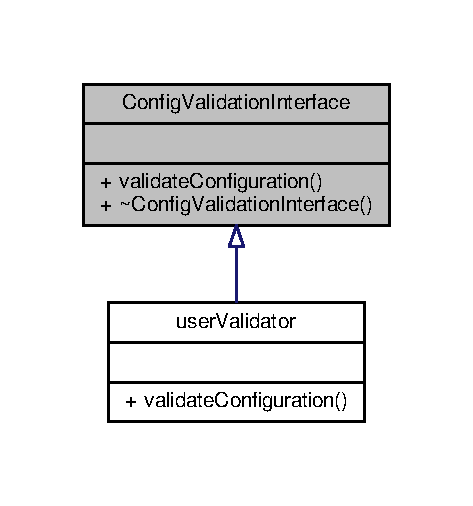
\includegraphics[width=227pt]{classConfigValidationInterface__inherit__graph}
\end{center}
\end{figure}


Collaboration diagram for Config\+Validation\+Interface\+:
\nopagebreak
\begin{figure}[H]
\begin{center}
\leavevmode
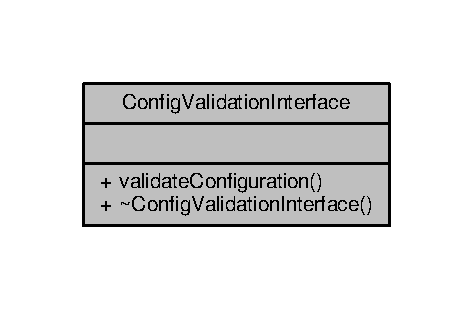
\includegraphics[width=227pt]{classConfigValidationInterface__coll__graph}
\end{center}
\end{figure}
\subsection*{Public Member Functions}
\begin{DoxyCompactItemize}
\item 
virtual bool \hyperlink{classConfigValidationInterface_a9f500c653a7b4b4559f920d499d7b96d}{validate\+Configuration} (\hyperlink{classConfigData}{Config\+Data} \&p\+Data)=0
\item 
virtual \hyperlink{classConfigValidationInterface_aaacb26c549e865004b61d51e3eadc105}{$\sim$\+Config\+Validation\+Interface} ()
\end{DoxyCompactItemize}


\subsection{Constructor \& Destructor Documentation}
\index{Config\+Validation\+Interface@{Config\+Validation\+Interface}!````~Config\+Validation\+Interface@{$\sim$\+Config\+Validation\+Interface}}
\index{````~Config\+Validation\+Interface@{$\sim$\+Config\+Validation\+Interface}!Config\+Validation\+Interface@{Config\+Validation\+Interface}}
\subsubsection[{\texorpdfstring{$\sim$\+Config\+Validation\+Interface()}{~ConfigValidationInterface()}}]{\setlength{\rightskip}{0pt plus 5cm}Config\+Validation\+Interface\+::$\sim$\+Config\+Validation\+Interface (
\begin{DoxyParamCaption}
{}
\end{DoxyParamCaption}
)\hspace{0.3cm}{\ttfamily [virtual]}}\hypertarget{classConfigValidationInterface_aaacb26c549e865004b61d51e3eadc105}{}\label{classConfigValidationInterface_aaacb26c549e865004b61d51e3eadc105}

\begin{DoxyCode}
17                                                       \{
18 \}
\end{DoxyCode}


\subsection{Member Function Documentation}
\index{Config\+Validation\+Interface@{Config\+Validation\+Interface}!validate\+Configuration@{validate\+Configuration}}
\index{validate\+Configuration@{validate\+Configuration}!Config\+Validation\+Interface@{Config\+Validation\+Interface}}
\subsubsection[{\texorpdfstring{validate\+Configuration(\+Config\+Data \&p\+Data)=0}{validateConfiguration(ConfigData &pData)=0}}]{\setlength{\rightskip}{0pt plus 5cm}virtual bool Config\+Validation\+Interface\+::validate\+Configuration (
\begin{DoxyParamCaption}
\item[{{\bf Config\+Data} \&}]{p\+Data}
\end{DoxyParamCaption}
)\hspace{0.3cm}{\ttfamily [pure virtual]}}\hypertarget{classConfigValidationInterface_a9f500c653a7b4b4559f920d499d7b96d}{}\label{classConfigValidationInterface_a9f500c653a7b4b4559f920d499d7b96d}


Implemented in \hyperlink{classuserValidator_ad496e5a1c1c183fb9ab04ac70f7d7b05}{user\+Validator}.



Referenced by rdf\+::\+Initializator\+::create\+Plataform().



The documentation for this class was generated from the following files\+:\begin{DoxyCompactItemize}
\item 
\hyperlink{ConfigValidationInterface_8h}{Config\+Validation\+Interface.\+h}\item 
\hyperlink{configValidator_8cpp}{config\+Validator.\+cpp}\end{DoxyCompactItemize}

\hypertarget{structEstructura_1_1DataMaster}{}\section{Estructura\+:\+:Data\+Master Struct Reference}
\label{structEstructura_1_1DataMaster}\index{Estructura\+::\+Data\+Master@{Estructura\+::\+Data\+Master}}


{\ttfamily \#include $<$Estructura.\+h$>$}



Collaboration diagram for Estructura\+:\+:Data\+Master\+:
\nopagebreak
\begin{figure}[H]
\begin{center}
\leavevmode
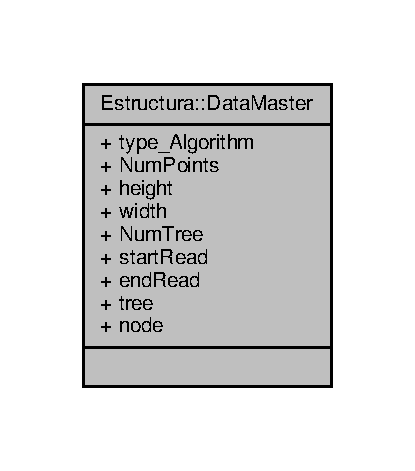
\includegraphics[width=199pt]{structEstructura_1_1DataMaster__coll__graph}
\end{center}
\end{figure}
\subsection*{Public Attributes}
\begin{DoxyCompactItemize}
\item 
std\+::string \hyperlink{structEstructura_1_1DataMaster_accae7ba56def5fd845b33cb8cfb384fe}{type\+\_\+\+Algorithm}
\item 
int \hyperlink{structEstructura_1_1DataMaster_ad62760f62256a3fbd88481f720b81851}{Num\+Points}
\item 
int \hyperlink{structEstructura_1_1DataMaster_a33df1604c867e22af955f29c453d6651}{height}
\item 
int \hyperlink{structEstructura_1_1DataMaster_a52e88b0d0d52d7e61880e3689ef2e638}{width}
\item 
int \hyperlink{structEstructura_1_1DataMaster_a950938f474870649fe7eceae940366fd}{Num\+Tree}
\item 
int \hyperlink{structEstructura_1_1DataMaster_ada49eb1401a3715858043ebd2b61c10c}{start\+Read}
\item 
int \hyperlink{structEstructura_1_1DataMaster_a787807eccc80c8e639d2409477f37f3a}{end\+Read}
\item 
int \hyperlink{structEstructura_1_1DataMaster_a766b1b437e0f242d3626a3759bef8b43}{tree}
\item 
int \hyperlink{structEstructura_1_1DataMaster_a5b7bf8e1c983ad0a64dd596d1bb4e31a}{node}
\end{DoxyCompactItemize}


\subsection{Member Data Documentation}
\index{Estructura\+::\+Data\+Master@{Estructura\+::\+Data\+Master}!end\+Read@{end\+Read}}
\index{end\+Read@{end\+Read}!Estructura\+::\+Data\+Master@{Estructura\+::\+Data\+Master}}
\subsubsection[{\texorpdfstring{end\+Read}{endRead}}]{\setlength{\rightskip}{0pt plus 5cm}int Estructura\+::\+Data\+Master\+::end\+Read}\hypertarget{structEstructura_1_1DataMaster_a787807eccc80c8e639d2409477f37f3a}{}\label{structEstructura_1_1DataMaster_a787807eccc80c8e639d2409477f37f3a}


Referenced by Image\+::get\+Structura(), and Image\+Manager\+::set\+Range().

\index{Estructura\+::\+Data\+Master@{Estructura\+::\+Data\+Master}!height@{height}}
\index{height@{height}!Estructura\+::\+Data\+Master@{Estructura\+::\+Data\+Master}}
\subsubsection[{\texorpdfstring{height}{height}}]{\setlength{\rightskip}{0pt plus 5cm}int Estructura\+::\+Data\+Master\+::height}\hypertarget{structEstructura_1_1DataMaster_a33df1604c867e22af955f29c453d6651}{}\label{structEstructura_1_1DataMaster_a33df1604c867e22af955f29c453d6651}


Referenced by Image\+::get\+Structura(), and Image\+Manager\+::\+Image\+Manager().

\index{Estructura\+::\+Data\+Master@{Estructura\+::\+Data\+Master}!node@{node}}
\index{node@{node}!Estructura\+::\+Data\+Master@{Estructura\+::\+Data\+Master}}
\subsubsection[{\texorpdfstring{node}{node}}]{\setlength{\rightskip}{0pt plus 5cm}int Estructura\+::\+Data\+Master\+::node}\hypertarget{structEstructura_1_1DataMaster_a5b7bf8e1c983ad0a64dd596d1bb4e31a}{}\label{structEstructura_1_1DataMaster_a5b7bf8e1c983ad0a64dd596d1bb4e31a}


Referenced by Image\+::get\+Structura(), and Image\+Manager\+::\+Image\+Manager().

\index{Estructura\+::\+Data\+Master@{Estructura\+::\+Data\+Master}!Num\+Points@{Num\+Points}}
\index{Num\+Points@{Num\+Points}!Estructura\+::\+Data\+Master@{Estructura\+::\+Data\+Master}}
\subsubsection[{\texorpdfstring{Num\+Points}{NumPoints}}]{\setlength{\rightskip}{0pt plus 5cm}int Estructura\+::\+Data\+Master\+::\+Num\+Points}\hypertarget{structEstructura_1_1DataMaster_ad62760f62256a3fbd88481f720b81851}{}\label{structEstructura_1_1DataMaster_ad62760f62256a3fbd88481f720b81851}


Referenced by Image\+::get\+Structura(), and Image\+Manager\+::\+Image\+Manager().

\index{Estructura\+::\+Data\+Master@{Estructura\+::\+Data\+Master}!Num\+Tree@{Num\+Tree}}
\index{Num\+Tree@{Num\+Tree}!Estructura\+::\+Data\+Master@{Estructura\+::\+Data\+Master}}
\subsubsection[{\texorpdfstring{Num\+Tree}{NumTree}}]{\setlength{\rightskip}{0pt plus 5cm}int Estructura\+::\+Data\+Master\+::\+Num\+Tree}\hypertarget{structEstructura_1_1DataMaster_a950938f474870649fe7eceae940366fd}{}\label{structEstructura_1_1DataMaster_a950938f474870649fe7eceae940366fd}


Referenced by Image\+::get\+Structura(), and Image\+Manager\+::\+Image\+Manager().

\index{Estructura\+::\+Data\+Master@{Estructura\+::\+Data\+Master}!start\+Read@{start\+Read}}
\index{start\+Read@{start\+Read}!Estructura\+::\+Data\+Master@{Estructura\+::\+Data\+Master}}
\subsubsection[{\texorpdfstring{start\+Read}{startRead}}]{\setlength{\rightskip}{0pt plus 5cm}int Estructura\+::\+Data\+Master\+::start\+Read}\hypertarget{structEstructura_1_1DataMaster_ada49eb1401a3715858043ebd2b61c10c}{}\label{structEstructura_1_1DataMaster_ada49eb1401a3715858043ebd2b61c10c}


Referenced by Image\+::get\+Structura(), and Image\+Manager\+::set\+Range().

\index{Estructura\+::\+Data\+Master@{Estructura\+::\+Data\+Master}!tree@{tree}}
\index{tree@{tree}!Estructura\+::\+Data\+Master@{Estructura\+::\+Data\+Master}}
\subsubsection[{\texorpdfstring{tree}{tree}}]{\setlength{\rightskip}{0pt plus 5cm}int Estructura\+::\+Data\+Master\+::tree}\hypertarget{structEstructura_1_1DataMaster_a766b1b437e0f242d3626a3759bef8b43}{}\label{structEstructura_1_1DataMaster_a766b1b437e0f242d3626a3759bef8b43}


Referenced by Image\+::get\+Structura(), and Image\+Manager\+::\+Image\+Manager().

\index{Estructura\+::\+Data\+Master@{Estructura\+::\+Data\+Master}!type\+\_\+\+Algorithm@{type\+\_\+\+Algorithm}}
\index{type\+\_\+\+Algorithm@{type\+\_\+\+Algorithm}!Estructura\+::\+Data\+Master@{Estructura\+::\+Data\+Master}}
\subsubsection[{\texorpdfstring{type\+\_\+\+Algorithm}{type_Algorithm}}]{\setlength{\rightskip}{0pt plus 5cm}std\+::string Estructura\+::\+Data\+Master\+::type\+\_\+\+Algorithm}\hypertarget{structEstructura_1_1DataMaster_accae7ba56def5fd845b33cb8cfb384fe}{}\label{structEstructura_1_1DataMaster_accae7ba56def5fd845b33cb8cfb384fe}


Referenced by Image\+::get\+Structura(), and Image\+Manager\+::\+Image\+Manager().

\index{Estructura\+::\+Data\+Master@{Estructura\+::\+Data\+Master}!width@{width}}
\index{width@{width}!Estructura\+::\+Data\+Master@{Estructura\+::\+Data\+Master}}
\subsubsection[{\texorpdfstring{width}{width}}]{\setlength{\rightskip}{0pt plus 5cm}int Estructura\+::\+Data\+Master\+::width}\hypertarget{structEstructura_1_1DataMaster_a52e88b0d0d52d7e61880e3689ef2e638}{}\label{structEstructura_1_1DataMaster_a52e88b0d0d52d7e61880e3689ef2e638}


Referenced by Image\+::get\+Structura(), and Image\+Manager\+::\+Image\+Manager().



The documentation for this struct was generated from the following file\+:\begin{DoxyCompactItemize}
\item 
\hyperlink{Estructura_8h}{Estructura.\+h}\end{DoxyCompactItemize}

\hypertarget{classDepthImage}{}\section{Depth\+Image Class Reference}
\label{classDepthImage}\index{Depth\+Image@{Depth\+Image}}


{\ttfamily \#include $<$Depth\+Image.\+h$>$}



Inheritance diagram for Depth\+Image\+:
\nopagebreak
\begin{figure}[H]
\begin{center}
\leavevmode
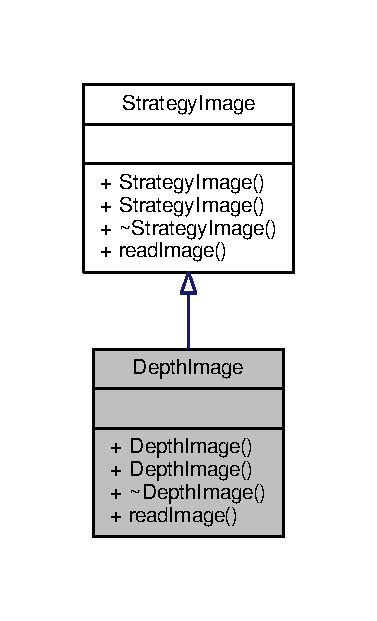
\includegraphics[width=181pt]{classDepthImage__inherit__graph}
\end{center}
\end{figure}


Collaboration diagram for Depth\+Image\+:
\nopagebreak
\begin{figure}[H]
\begin{center}
\leavevmode
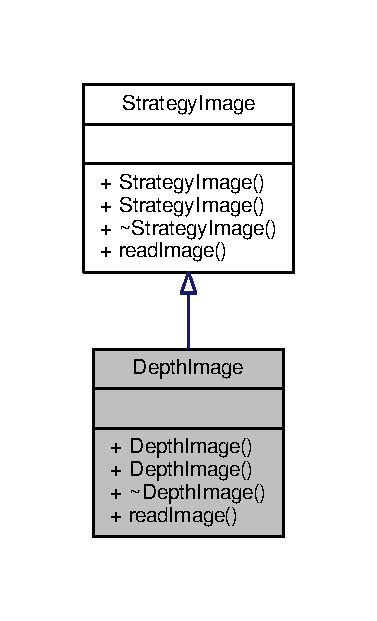
\includegraphics[width=181pt]{classDepthImage__coll__graph}
\end{center}
\end{figure}
\subsection*{Public Member Functions}
\begin{DoxyCompactItemize}
\item 
\hyperlink{classDepthImage_a3a391f24f9fa8480026b5c6e75ea8ae0}{Depth\+Image} ()
\item 
\hyperlink{classDepthImage_ae7b2b3cb66c4ee32426718d1034117f3}{Depth\+Image} (const \hyperlink{classDepthImage}{Depth\+Image} \&orig)
\item 
virtual \hyperlink{classDepthImage_aef27b02feac32d27dade770bd9a6638c}{$\sim$\+Depth\+Image} ()
\item 
virtual void \hyperlink{classDepthImage_a07e7b06393e869a1cc3c5b39d2dcdad0}{read\+Image} (int height, int width, std\+::string direction, cv\+::\+Mat \&image)
\end{DoxyCompactItemize}


\subsection{Constructor \& Destructor Documentation}
\index{Depth\+Image@{Depth\+Image}!Depth\+Image@{Depth\+Image}}
\index{Depth\+Image@{Depth\+Image}!Depth\+Image@{Depth\+Image}}
\subsubsection[{\texorpdfstring{Depth\+Image()}{DepthImage()}}]{\setlength{\rightskip}{0pt plus 5cm}Depth\+Image\+::\+Depth\+Image (
\begin{DoxyParamCaption}
{}
\end{DoxyParamCaption}
)}\hypertarget{classDepthImage_a3a391f24f9fa8480026b5c6e75ea8ae0}{}\label{classDepthImage_a3a391f24f9fa8480026b5c6e75ea8ae0}

\begin{DoxyCode}
16                        \{
17 \}
\end{DoxyCode}
\index{Depth\+Image@{Depth\+Image}!Depth\+Image@{Depth\+Image}}
\index{Depth\+Image@{Depth\+Image}!Depth\+Image@{Depth\+Image}}
\subsubsection[{\texorpdfstring{Depth\+Image(const Depth\+Image \&orig)}{DepthImage(const DepthImage &orig)}}]{\setlength{\rightskip}{0pt plus 5cm}Depth\+Image\+::\+Depth\+Image (
\begin{DoxyParamCaption}
\item[{const {\bf Depth\+Image} \&}]{orig}
\end{DoxyParamCaption}
)}\hypertarget{classDepthImage_ae7b2b3cb66c4ee32426718d1034117f3}{}\label{classDepthImage_ae7b2b3cb66c4ee32426718d1034117f3}

\begin{DoxyCode}
19                                              \{
20 \}
\end{DoxyCode}
\index{Depth\+Image@{Depth\+Image}!````~Depth\+Image@{$\sim$\+Depth\+Image}}
\index{````~Depth\+Image@{$\sim$\+Depth\+Image}!Depth\+Image@{Depth\+Image}}
\subsubsection[{\texorpdfstring{$\sim$\+Depth\+Image()}{~DepthImage()}}]{\setlength{\rightskip}{0pt plus 5cm}Depth\+Image\+::$\sim$\+Depth\+Image (
\begin{DoxyParamCaption}
{}
\end{DoxyParamCaption}
)\hspace{0.3cm}{\ttfamily [virtual]}}\hypertarget{classDepthImage_aef27b02feac32d27dade770bd9a6638c}{}\label{classDepthImage_aef27b02feac32d27dade770bd9a6638c}

\begin{DoxyCode}
22                         \{
23 \}
\end{DoxyCode}


\subsection{Member Function Documentation}
\index{Depth\+Image@{Depth\+Image}!read\+Image@{read\+Image}}
\index{read\+Image@{read\+Image}!Depth\+Image@{Depth\+Image}}
\subsubsection[{\texorpdfstring{read\+Image(int height, int width, std\+::string direction, cv\+::\+Mat \&image)}{readImage(int height, int width, std::string direction, cv::Mat &image)}}]{\setlength{\rightskip}{0pt plus 5cm}void Depth\+Image\+::read\+Image (
\begin{DoxyParamCaption}
\item[{int}]{height, }
\item[{int}]{width, }
\item[{std\+::string}]{direction, }
\item[{cv\+::\+Mat \&}]{image}
\end{DoxyParamCaption}
)\hspace{0.3cm}{\ttfamily [virtual]}}\hypertarget{classDepthImage_a07e7b06393e869a1cc3c5b39d2dcdad0}{}\label{classDepthImage_a07e7b06393e869a1cc3c5b39d2dcdad0}
Funcion para la lectura de la imagen de profundidad. 
\begin{DoxyParams}{Parameters}
{\em direction} & \\
\hline
{\em image\+Label} & \\
\hline
\end{DoxyParams}


Implements \hyperlink{classStrategyImage_aee857e79df483412f66b529417ddfd44}{Strategy\+Image}.


\begin{DoxyCode}
29                                                                                    \{
30     cv::Mat imegeDepth;
31     imegeDepth = cv::Mat(height, width, CV\_16UC1, cv::Scalar(0));
32     std::string rute = direction;
33     imegeDepth = cv::imread(rute.c\_str(),CV\_16UC1);
34     image = imegeDepth;
35 \}\end{DoxyCode}


The documentation for this class was generated from the following files\+:\begin{DoxyCompactItemize}
\item 
\hyperlink{DepthImage_8h}{Depth\+Image.\+h}\item 
\hyperlink{DepthImage_8cpp}{Depth\+Image.\+cpp}\end{DoxyCompactItemize}

\hypertarget{classrdf_1_1DistributionManager}{}\section{rdf\+:\+:Distribution\+Manager Class Reference}
\label{classrdf_1_1DistributionManager}\index{rdf\+::\+Distribution\+Manager@{rdf\+::\+Distribution\+Manager}}


{\ttfamily \#include $<$Distribution\+Manager.\+h$>$}



Collaboration diagram for rdf\+:\+:Distribution\+Manager\+:
\nopagebreak
\begin{figure}[H]
\begin{center}
\leavevmode
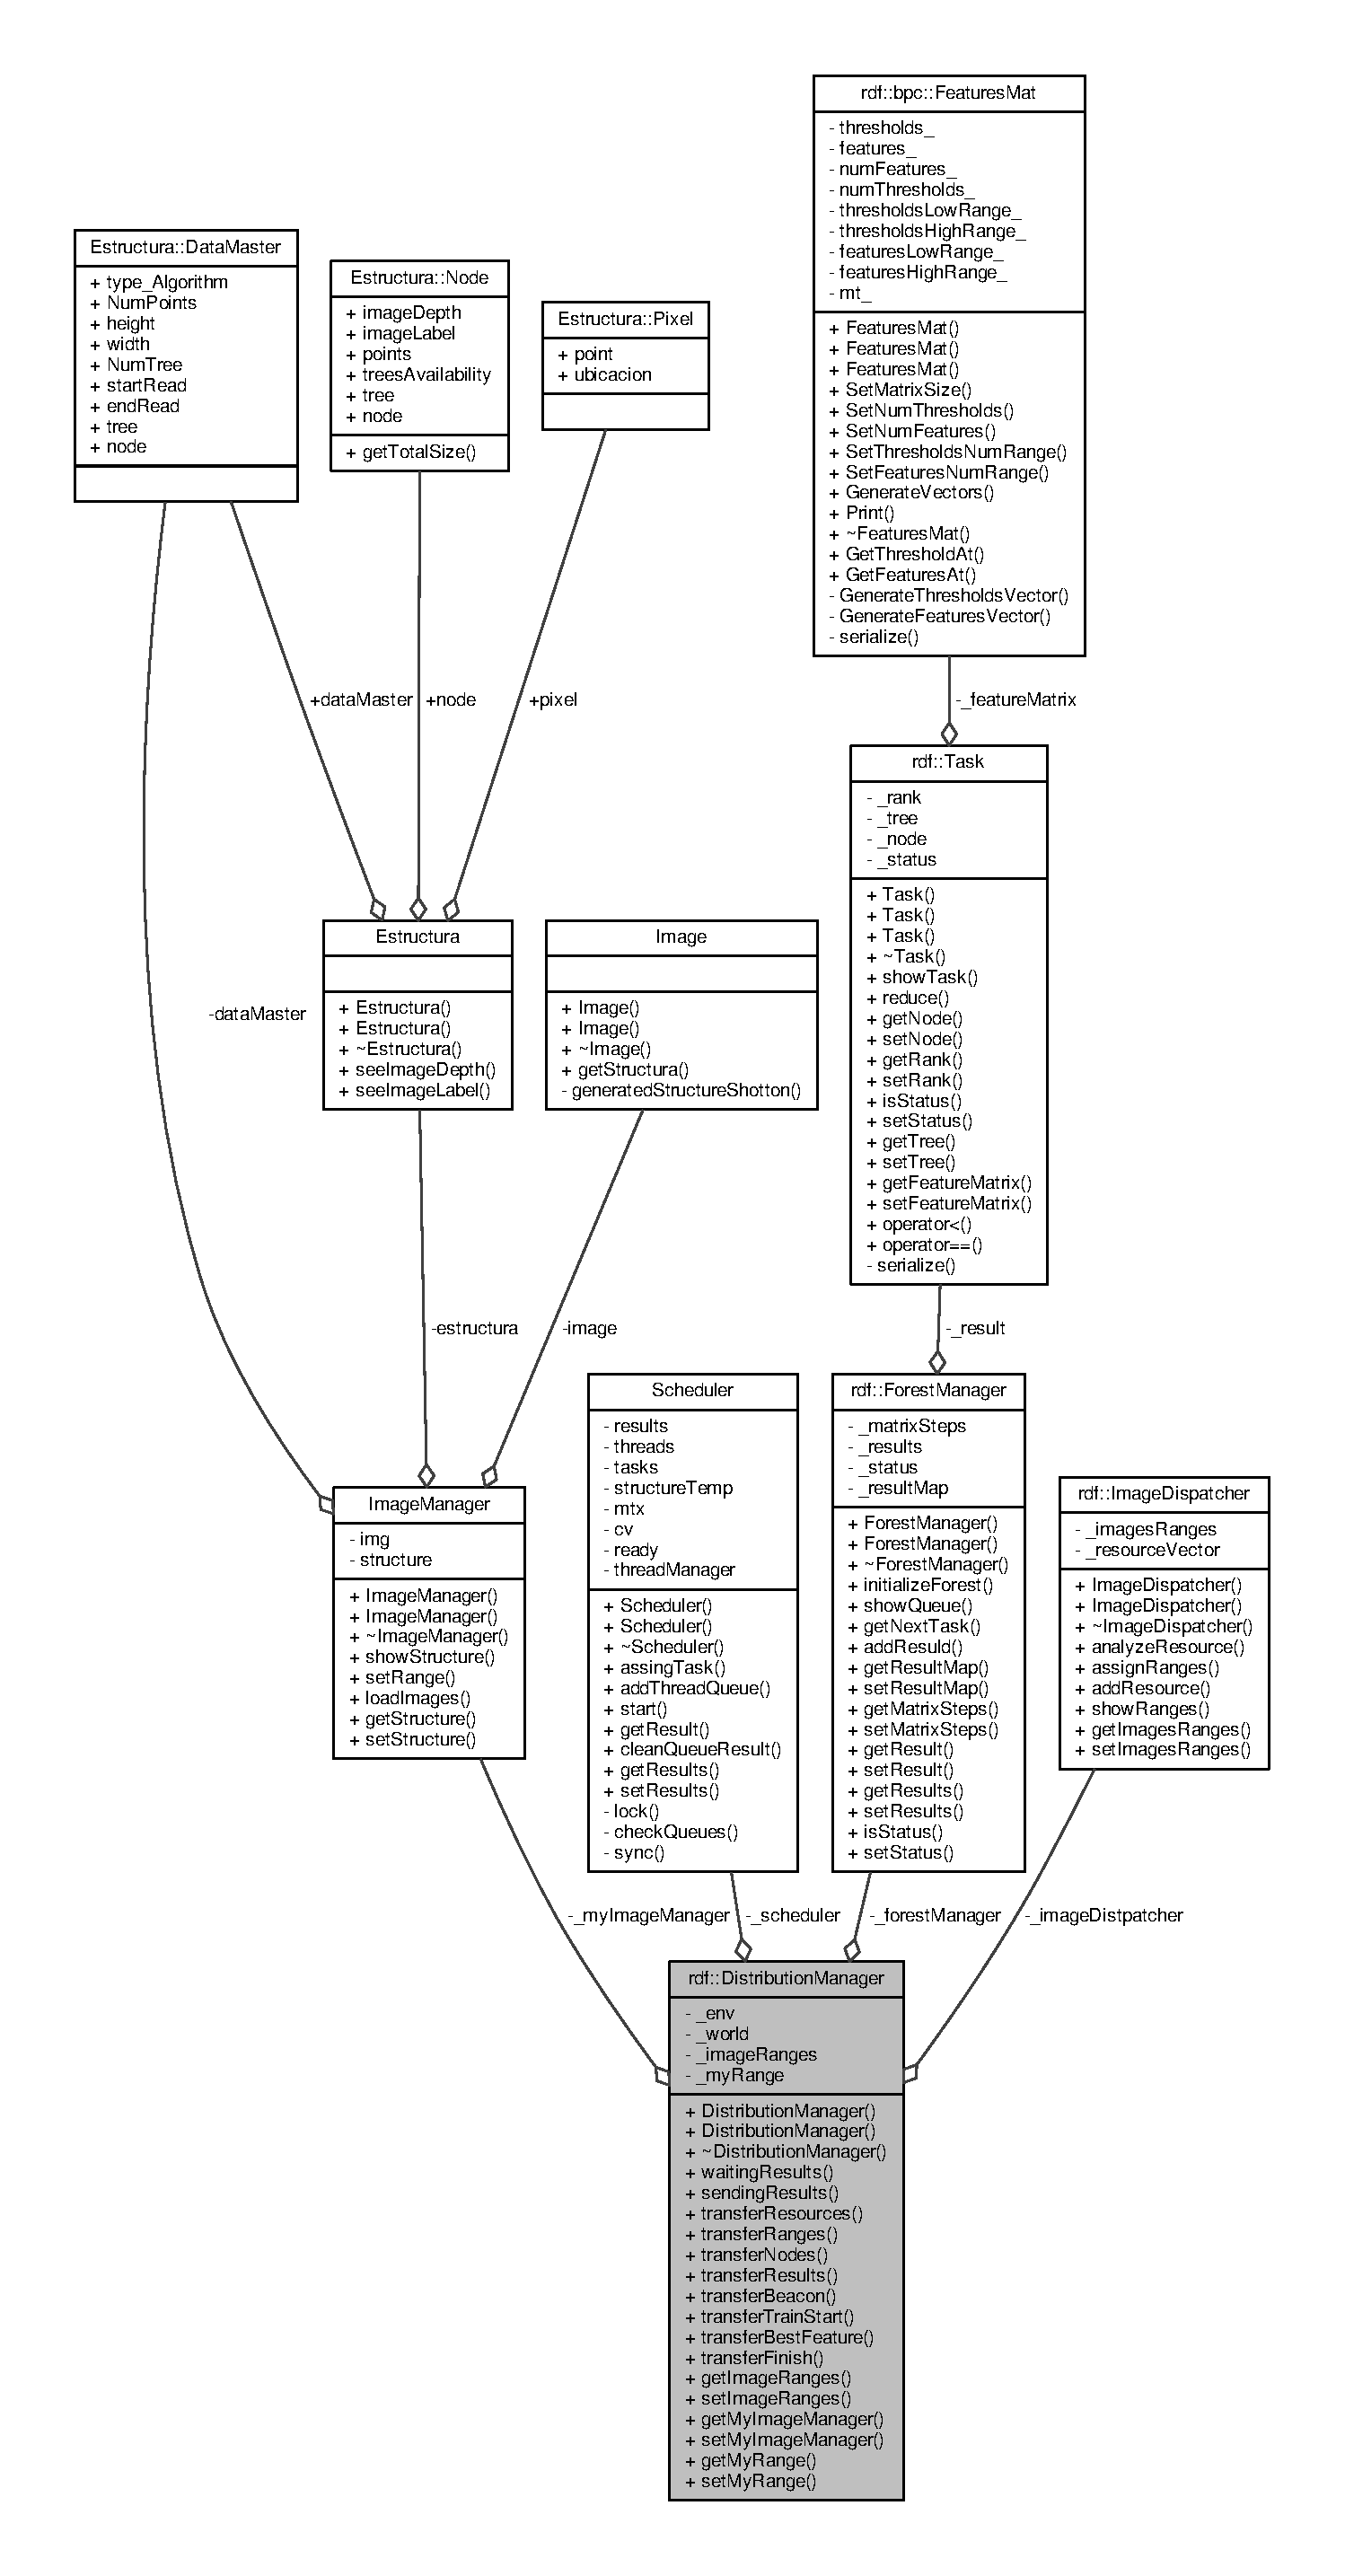
\includegraphics[height=550pt]{classrdf_1_1DistributionManager__coll__graph}
\end{center}
\end{figure}
\subsection*{Public Member Functions}
\begin{DoxyCompactItemize}
\item 
\hyperlink{classrdf_1_1DistributionManager_ad305a637e032d254c3884911294919e4}{Distribution\+Manager} ()
\item 
\hyperlink{classrdf_1_1DistributionManager_ab0df571638e2f1a645a6b10a46be43dc}{Distribution\+Manager} (const \hyperlink{classrdf_1_1DistributionManager}{Distribution\+Manager} \&orig)
\item 
virtual \hyperlink{classrdf_1_1DistributionManager_a5165d8567d99652270a892b576bc8d41}{$\sim$\+Distribution\+Manager} ()
\item 
void \hyperlink{classrdf_1_1DistributionManager_ad030f06a725590893f186cf95df7ed19}{waiting\+Results} ()
\item 
void \hyperlink{classrdf_1_1DistributionManager_aaa23849f108cf3199eb6a076c37a269c}{sending\+Results} ()
\item 
void \hyperlink{classrdf_1_1DistributionManager_aee4c4143848ea57742d79f8ee137b4c7}{transfer\+Resources} ()
\item 
void \hyperlink{classrdf_1_1DistributionManager_af601ca87a8a5b21632e5c70de253d8cb}{transfer\+Ranges} ()
\item 
void \hyperlink{classrdf_1_1DistributionManager_ac98b0403d6311d00e7b95c03fa4aa0f3}{transfer\+Nodes} (\hyperlink{classrdf_1_1Task}{Task} \&p\+Task)
\item 
void \hyperlink{classrdf_1_1DistributionManager_a16efc159bccc8c621d28d62310cfb2e0}{transfer\+Results} ()
\item 
void \hyperlink{classrdf_1_1DistributionManager_a30ac28e002aebe633229c993a65437fd}{transfer\+Beacon} ()
\item 
void \hyperlink{classrdf_1_1DistributionManager_a7430723023243687df8181b7575cb167}{transfer\+Train\+Start} (\hyperlink{classrdf_1_1ForestManager}{Forest\+Manager} \&p\+Forest)
\item 
void \hyperlink{classrdf_1_1DistributionManager_ab28b3c19afaae2917fdac53f426b1835}{transfer\+Best\+Feature} (\hyperlink{classrdf_1_1bpc_1_1BestFeatureMsg}{rdf\+::bpc\+::\+Best\+Feature\+Msg} p\+Feature)
\item 
void \hyperlink{classrdf_1_1DistributionManager_acc9fe7a5966360e5e82d916a0eed1712}{transfer\+Finish} ()
\item 
std\+::vector$<$ std\+::pair$<$ int, int $>$ $>$ \hyperlink{classrdf_1_1DistributionManager_a31ba2ded77d4addc0a245daf08e6a704}{get\+Image\+Ranges} () const 
\item 
void \hyperlink{classrdf_1_1DistributionManager_a3545e401850b0263252d07c815220b13}{set\+Image\+Ranges} (std\+::vector$<$ std\+::pair$<$ int, int $>$ $>$ \hyperlink{classrdf_1_1DistributionManager_a5f3f6245bed7bfcf34204fc16e655656}{\+\_\+image\+Ranges})
\item 
\hyperlink{classImageManager}{Image\+Manager} \hyperlink{classrdf_1_1DistributionManager_a264664d495909f826523699558d4f8e4}{get\+My\+Image\+Manager} () const 
\item 
void \hyperlink{classrdf_1_1DistributionManager_aebde88548a718fc7b984ff356abebd27}{set\+My\+Image\+Manager} (\hyperlink{classImageManager}{Image\+Manager} \hyperlink{classrdf_1_1DistributionManager_aa265ab894795aa960fdcc67f0934934f}{\+\_\+my\+Image\+Manager})
\item 
pair$<$ int, int $>$ \hyperlink{classrdf_1_1DistributionManager_a5fcb2947236b8109c575215c15b55791}{get\+My\+Range} () const 
\item 
void \hyperlink{classrdf_1_1DistributionManager_a8c137d7196f9876c9079f7ef7a9dd8f5}{set\+My\+Range} (pair$<$ int, int $>$ \hyperlink{classrdf_1_1DistributionManager_ac6e764a519add6afff6ba14e09e45cfa}{\+\_\+my\+Range})
\end{DoxyCompactItemize}
\subsection*{Private Attributes}
\begin{DoxyCompactItemize}
\item 
mpi\+::environment \hyperlink{classrdf_1_1DistributionManager_ab24e19df5707be063ee48ef9f41af13f}{\+\_\+env}
\item 
mpi\+::communicator \hyperlink{classrdf_1_1DistributionManager_ac8a061176717baf96b2913cd22dcbf20}{\+\_\+world}
\item 
std\+::vector$<$ std\+::pair$<$ int, int $>$ $>$ \hyperlink{classrdf_1_1DistributionManager_a5f3f6245bed7bfcf34204fc16e655656}{\+\_\+image\+Ranges}
\item 
pair$<$ int, int $>$ \hyperlink{classrdf_1_1DistributionManager_ac6e764a519add6afff6ba14e09e45cfa}{\+\_\+my\+Range}
\item 
\hyperlink{classImageManager}{Image\+Manager} \hyperlink{classrdf_1_1DistributionManager_aa265ab894795aa960fdcc67f0934934f}{\+\_\+my\+Image\+Manager}
\item 
\hyperlink{classrdf_1_1ForestManager}{rdf\+::\+Forest\+Manager} \hyperlink{classrdf_1_1DistributionManager_aba2daa8780c7915f9f1a5d871edb93c9}{\+\_\+forest\+Manager}
\item 
\hyperlink{classrdf_1_1ImageDispatcher}{rdf\+::\+Image\+Dispatcher} \hyperlink{classrdf_1_1DistributionManager_a43d6497690b1040281e7dfd64ed4dc65}{\+\_\+image\+Distpatcher}
\item 
\hyperlink{classScheduler}{Scheduler} \hyperlink{classrdf_1_1DistributionManager_a6a628c16669a4c94837597193fa95ecb}{\+\_\+scheduler}
\end{DoxyCompactItemize}


\subsection{Detailed Description}
Class that works on distribute all messages within M\+P\+I.\+B\+O\+O\+ST 

\subsection{Constructor \& Destructor Documentation}
\index{rdf\+::\+Distribution\+Manager@{rdf\+::\+Distribution\+Manager}!Distribution\+Manager@{Distribution\+Manager}}
\index{Distribution\+Manager@{Distribution\+Manager}!rdf\+::\+Distribution\+Manager@{rdf\+::\+Distribution\+Manager}}
\subsubsection[{\texorpdfstring{Distribution\+Manager()}{DistributionManager()}}]{\setlength{\rightskip}{0pt plus 5cm}rdf\+::\+Distribution\+Manager\+::\+Distribution\+Manager (
\begin{DoxyParamCaption}
{}
\end{DoxyParamCaption}
)}\hypertarget{classrdf_1_1DistributionManager_ad305a637e032d254c3884911294919e4}{}\label{classrdf_1_1DistributionManager_ad305a637e032d254c3884911294919e4}

\begin{DoxyCode}
22 \{\}
\end{DoxyCode}
\index{rdf\+::\+Distribution\+Manager@{rdf\+::\+Distribution\+Manager}!Distribution\+Manager@{Distribution\+Manager}}
\index{Distribution\+Manager@{Distribution\+Manager}!rdf\+::\+Distribution\+Manager@{rdf\+::\+Distribution\+Manager}}
\subsubsection[{\texorpdfstring{Distribution\+Manager(const Distribution\+Manager \&orig)}{DistributionManager(const DistributionManager &orig)}}]{\setlength{\rightskip}{0pt plus 5cm}rdf\+::\+Distribution\+Manager\+::\+Distribution\+Manager (
\begin{DoxyParamCaption}
\item[{const {\bf Distribution\+Manager} \&}]{orig}
\end{DoxyParamCaption}
)}\hypertarget{classrdf_1_1DistributionManager_ab0df571638e2f1a645a6b10a46be43dc}{}\label{classrdf_1_1DistributionManager_ab0df571638e2f1a645a6b10a46be43dc}


References \+\_\+image\+Ranges, \+\_\+my\+Image\+Manager, and \+\_\+my\+Range.


\begin{DoxyCode}
23                                                                            \{
24     \hyperlink{classrdf_1_1DistributionManager_a5f3f6245bed7bfcf34204fc16e655656}{\_imageRanges}    = orig.\_imageRanges;
25     \hyperlink{classrdf_1_1DistributionManager_aa265ab894795aa960fdcc67f0934934f}{\_myImageManager} = orig.\_myImageManager;
26     \hyperlink{classrdf_1_1DistributionManager_ac6e764a519add6afff6ba14e09e45cfa}{\_myRange}        = orig.\_myRange;        
27 \}
\end{DoxyCode}
\index{rdf\+::\+Distribution\+Manager@{rdf\+::\+Distribution\+Manager}!````~Distribution\+Manager@{$\sim$\+Distribution\+Manager}}
\index{````~Distribution\+Manager@{$\sim$\+Distribution\+Manager}!rdf\+::\+Distribution\+Manager@{rdf\+::\+Distribution\+Manager}}
\subsubsection[{\texorpdfstring{$\sim$\+Distribution\+Manager()}{~DistributionManager()}}]{\setlength{\rightskip}{0pt plus 5cm}rdf\+::\+Distribution\+Manager\+::$\sim$\+Distribution\+Manager (
\begin{DoxyParamCaption}
{}
\end{DoxyParamCaption}
)\hspace{0.3cm}{\ttfamily [virtual]}}\hypertarget{classrdf_1_1DistributionManager_a5165d8567d99652270a892b576bc8d41}{}\label{classrdf_1_1DistributionManager_a5165d8567d99652270a892b576bc8d41}

\begin{DoxyCode}
28 \{\}
\end{DoxyCode}


\subsection{Member Function Documentation}
\index{rdf\+::\+Distribution\+Manager@{rdf\+::\+Distribution\+Manager}!get\+Image\+Ranges@{get\+Image\+Ranges}}
\index{get\+Image\+Ranges@{get\+Image\+Ranges}!rdf\+::\+Distribution\+Manager@{rdf\+::\+Distribution\+Manager}}
\subsubsection[{\texorpdfstring{get\+Image\+Ranges() const }{getImageRanges() const }}]{\setlength{\rightskip}{0pt plus 5cm}std\+::vector$<$std\+::pair$<$int, int$>$ $>$ rdf\+::\+Distribution\+Manager\+::get\+Image\+Ranges (
\begin{DoxyParamCaption}
{}
\end{DoxyParamCaption}
) const\hspace{0.3cm}{\ttfamily [inline]}}\hypertarget{classrdf_1_1DistributionManager_a31ba2ded77d4addc0a245daf08e6a704}{}\label{classrdf_1_1DistributionManager_a31ba2ded77d4addc0a245daf08e6a704}
G\+E\+T\+T\+E\+RS A\+ND S\+E\+T\+T\+E\+RS F\+OR M\+A\+IN V\+A\+R\+I\+A\+B\+L\+ES 

References \+\_\+image\+Ranges.


\begin{DoxyCode}
89                                                              \{
90             \textcolor{keywordflow}{return} \hyperlink{classrdf_1_1DistributionManager_a5f3f6245bed7bfcf34204fc16e655656}{\_imageRanges};
91         \}
\end{DoxyCode}
\index{rdf\+::\+Distribution\+Manager@{rdf\+::\+Distribution\+Manager}!get\+My\+Image\+Manager@{get\+My\+Image\+Manager}}
\index{get\+My\+Image\+Manager@{get\+My\+Image\+Manager}!rdf\+::\+Distribution\+Manager@{rdf\+::\+Distribution\+Manager}}
\subsubsection[{\texorpdfstring{get\+My\+Image\+Manager() const }{getMyImageManager() const }}]{\setlength{\rightskip}{0pt plus 5cm}{\bf Image\+Manager} rdf\+::\+Distribution\+Manager\+::get\+My\+Image\+Manager (
\begin{DoxyParamCaption}
{}
\end{DoxyParamCaption}
) const\hspace{0.3cm}{\ttfamily [inline]}}\hypertarget{classrdf_1_1DistributionManager_a264664d495909f826523699558d4f8e4}{}\label{classrdf_1_1DistributionManager_a264664d495909f826523699558d4f8e4}


References \+\_\+my\+Image\+Manager.


\begin{DoxyCode}
96                                                \{
97             \textcolor{keywordflow}{return} \hyperlink{classrdf_1_1DistributionManager_aa265ab894795aa960fdcc67f0934934f}{\_myImageManager};
98         \}
\end{DoxyCode}
\index{rdf\+::\+Distribution\+Manager@{rdf\+::\+Distribution\+Manager}!get\+My\+Range@{get\+My\+Range}}
\index{get\+My\+Range@{get\+My\+Range}!rdf\+::\+Distribution\+Manager@{rdf\+::\+Distribution\+Manager}}
\subsubsection[{\texorpdfstring{get\+My\+Range() const }{getMyRange() const }}]{\setlength{\rightskip}{0pt plus 5cm}pair$<$int, int$>$ rdf\+::\+Distribution\+Manager\+::get\+My\+Range (
\begin{DoxyParamCaption}
{}
\end{DoxyParamCaption}
) const\hspace{0.3cm}{\ttfamily [inline]}}\hypertarget{classrdf_1_1DistributionManager_a5fcb2947236b8109c575215c15b55791}{}\label{classrdf_1_1DistributionManager_a5fcb2947236b8109c575215c15b55791}


References \+\_\+my\+Range.


\begin{DoxyCode}
104                                           \{
105             \textcolor{keywordflow}{return} \hyperlink{classrdf_1_1DistributionManager_ac6e764a519add6afff6ba14e09e45cfa}{\_myRange};
106         \}
\end{DoxyCode}
\index{rdf\+::\+Distribution\+Manager@{rdf\+::\+Distribution\+Manager}!sending\+Results@{sending\+Results}}
\index{sending\+Results@{sending\+Results}!rdf\+::\+Distribution\+Manager@{rdf\+::\+Distribution\+Manager}}
\subsubsection[{\texorpdfstring{sending\+Results()}{sendingResults()}}]{\setlength{\rightskip}{0pt plus 5cm}void rdf\+::\+Distribution\+Manager\+::sending\+Results (
\begin{DoxyParamCaption}
{}
\end{DoxyParamCaption}
)}\hypertarget{classrdf_1_1DistributionManager_aaa23849f108cf3199eb6a076c37a269c}{}\label{classrdf_1_1DistributionManager_aaa23849f108cf3199eb6a076c37a269c}


References \+\_\+scheduler, \+\_\+world, and Scheduler\+::get\+Results().



Referenced by transfer\+Results().


\begin{DoxyCode}
42                                             \{
43     \textcolor{keywordflow}{while}(\textcolor{keyword}{true})\{
44         
45         \textcolor{keywordflow}{if}(!\hyperlink{classrdf_1_1DistributionManager_a6a628c16669a4c94837597193fa95ecb}{\_scheduler}.\hyperlink{classScheduler_a8864f6b658cf4d2a6d9d78a84c6d81f7}{getResults}().empty()) \{
46             std::cout << \textcolor{stringliteral}{"SENDING THREAD \(\backslash\)n"};
47             \hyperlink{classrdf_1_1DistributionManager_ac8a061176717baf96b2913cd22dcbf20}{\_world}.send(0, 2,\hyperlink{classrdf_1_1DistributionManager_a6a628c16669a4c94837597193fa95ecb}{\_scheduler}.\hyperlink{classScheduler_a8864f6b658cf4d2a6d9d78a84c6d81f7}{getResults}().front()) ; 
48             \hyperlink{classrdf_1_1DistributionManager_a6a628c16669a4c94837597193fa95ecb}{\_scheduler}.\hyperlink{classScheduler_a8864f6b658cf4d2a6d9d78a84c6d81f7}{getResults}().pop();
49             
50         \}
51     \}
52 \}
\end{DoxyCode}
\index{rdf\+::\+Distribution\+Manager@{rdf\+::\+Distribution\+Manager}!set\+Image\+Ranges@{set\+Image\+Ranges}}
\index{set\+Image\+Ranges@{set\+Image\+Ranges}!rdf\+::\+Distribution\+Manager@{rdf\+::\+Distribution\+Manager}}
\subsubsection[{\texorpdfstring{set\+Image\+Ranges(std\+::vector$<$ std\+::pair$<$ int, int $>$ $>$ \+\_\+image\+Ranges)}{setImageRanges(std::vector< std::pair< int, int > > _imageRanges)}}]{\setlength{\rightskip}{0pt plus 5cm}void rdf\+::\+Distribution\+Manager\+::set\+Image\+Ranges (
\begin{DoxyParamCaption}
\item[{std\+::vector$<$ std\+::pair$<$ int, int $>$ $>$}]{\+\_\+image\+Ranges}
\end{DoxyParamCaption}
)\hspace{0.3cm}{\ttfamily [inline]}}\hypertarget{classrdf_1_1DistributionManager_a3545e401850b0263252d07c815220b13}{}\label{classrdf_1_1DistributionManager_a3545e401850b0263252d07c815220b13}


References \+\_\+image\+Ranges.


\begin{DoxyCode}
93                                                                         \{
94             this->\hyperlink{classrdf_1_1DistributionManager_a5f3f6245bed7bfcf34204fc16e655656}{\_imageRanges} = \hyperlink{classrdf_1_1DistributionManager_a5f3f6245bed7bfcf34204fc16e655656}{\_imageRanges};
95         \}
\end{DoxyCode}
\index{rdf\+::\+Distribution\+Manager@{rdf\+::\+Distribution\+Manager}!set\+My\+Image\+Manager@{set\+My\+Image\+Manager}}
\index{set\+My\+Image\+Manager@{set\+My\+Image\+Manager}!rdf\+::\+Distribution\+Manager@{rdf\+::\+Distribution\+Manager}}
\subsubsection[{\texorpdfstring{set\+My\+Image\+Manager(\+Image\+Manager \+\_\+my\+Image\+Manager)}{setMyImageManager(ImageManager _myImageManager)}}]{\setlength{\rightskip}{0pt plus 5cm}void rdf\+::\+Distribution\+Manager\+::set\+My\+Image\+Manager (
\begin{DoxyParamCaption}
\item[{{\bf Image\+Manager}}]{\+\_\+my\+Image\+Manager}
\end{DoxyParamCaption}
)\hspace{0.3cm}{\ttfamily [inline]}}\hypertarget{classrdf_1_1DistributionManager_aebde88548a718fc7b984ff356abebd27}{}\label{classrdf_1_1DistributionManager_aebde88548a718fc7b984ff356abebd27}


References \+\_\+my\+Image\+Manager.


\begin{DoxyCode}
100                                                              \{
101             this->\_myImageManager = \hyperlink{classrdf_1_1DistributionManager_aa265ab894795aa960fdcc67f0934934f}{\_myImageManager};
102         \}
\end{DoxyCode}
\index{rdf\+::\+Distribution\+Manager@{rdf\+::\+Distribution\+Manager}!set\+My\+Range@{set\+My\+Range}}
\index{set\+My\+Range@{set\+My\+Range}!rdf\+::\+Distribution\+Manager@{rdf\+::\+Distribution\+Manager}}
\subsubsection[{\texorpdfstring{set\+My\+Range(pair$<$ int, int $>$ \+\_\+my\+Range)}{setMyRange(pair< int, int > _myRange)}}]{\setlength{\rightskip}{0pt plus 5cm}void rdf\+::\+Distribution\+Manager\+::set\+My\+Range (
\begin{DoxyParamCaption}
\item[{pair$<$ int, int $>$}]{\+\_\+my\+Range}
\end{DoxyParamCaption}
)\hspace{0.3cm}{\ttfamily [inline]}}\hypertarget{classrdf_1_1DistributionManager_a8c137d7196f9876c9079f7ef7a9dd8f5}{}\label{classrdf_1_1DistributionManager_a8c137d7196f9876c9079f7ef7a9dd8f5}


References \+\_\+my\+Range.


\begin{DoxyCode}
108                                                  \{
109             this->\hyperlink{classrdf_1_1DistributionManager_ac6e764a519add6afff6ba14e09e45cfa}{\_myRange} = \hyperlink{classrdf_1_1DistributionManager_ac6e764a519add6afff6ba14e09e45cfa}{\_myRange};
110         \}
\end{DoxyCode}
\index{rdf\+::\+Distribution\+Manager@{rdf\+::\+Distribution\+Manager}!transfer\+Beacon@{transfer\+Beacon}}
\index{transfer\+Beacon@{transfer\+Beacon}!rdf\+::\+Distribution\+Manager@{rdf\+::\+Distribution\+Manager}}
\subsubsection[{\texorpdfstring{transfer\+Beacon()}{transferBeacon()}}]{\setlength{\rightskip}{0pt plus 5cm}void rdf\+::\+Distribution\+Manager\+::transfer\+Beacon (
\begin{DoxyParamCaption}
{}
\end{DoxyParamCaption}
)}\hypertarget{classrdf_1_1DistributionManager_a30ac28e002aebe633229c993a65437fd}{}\label{classrdf_1_1DistributionManager_a30ac28e002aebe633229c993a65437fd}
This messages is to ensure that all the process are running alive. 

References \+\_\+world.


\begin{DoxyCode}
160                                             \{
161     \textcolor{keywordflow}{if} (\hyperlink{classrdf_1_1DistributionManager_ac8a061176717baf96b2913cd22dcbf20}{\_world}.size() <= 1) \{
162     std::cout << \textcolor{stringliteral}{"Need more than 1 processes to play around."} << std::endl;
163     \}
164     \textcolor{keywordflow}{else} \{ 
165         \textcolor{keywordflow}{if}(\hyperlink{classrdf_1_1DistributionManager_ac8a061176717baf96b2913cd22dcbf20}{\_world}.rank() == 0)\{                                         \textcolor{comment}{// MASTER PROCESS}
166             std::string log = \textcolor{stringliteral}{"logInfo"};                               
167             broadcast(\hyperlink{classrdf_1_1DistributionManager_ac8a061176717baf96b2913cd22dcbf20}{\_world}, log, 0);                                  \textcolor{comment}{// Send the task to every
       process in the cluster}
168             std::cout << \textcolor{stringliteral}{"Master asking for log info log\(\backslash\)n"};
169             std::string response;
170             \textcolor{keywordtype}{int} i = 1;
171             \textcolor{keywordflow}{do} \{                                                        \textcolor{comment}{// Wait all the responses }
172                 \hyperlink{classrdf_1_1DistributionManager_ac8a061176717baf96b2913cd22dcbf20}{\_world}.recv(boost::mpi::any\_source, boost::mpi::any\_tag,response);
173                 std::cout << \textcolor{stringliteral}{"Master Receive log information "} << response  << \textcolor{stringliteral}{"\(\backslash\)n"};
174                 i++;
175             \}\textcolor{keywordflow}{while}(i<\hyperlink{classrdf_1_1DistributionManager_ac8a061176717baf96b2913cd22dcbf20}{\_world}.size()); 
176         \}    
177         \textcolor{keywordflow}{else} \{
178             std::string logInfo;
179             \hyperlink{classrdf_1_1DistributionManager_ac8a061176717baf96b2913cd22dcbf20}{\_world}.recv(boost::mpi::any\_source, boost::mpi::any\_tag, logInfo);
180             std::string response = \textcolor{stringliteral}{"LOG\_"} + std::to\_string(\hyperlink{classrdf_1_1DistributionManager_ac8a061176717baf96b2913cd22dcbf20}{\_world}.rank());
181             \hyperlink{classrdf_1_1DistributionManager_ac8a061176717baf96b2913cd22dcbf20}{\_world}.send(0,0,response);
182         \}
183     \}
184 
185 \}
\end{DoxyCode}
\index{rdf\+::\+Distribution\+Manager@{rdf\+::\+Distribution\+Manager}!transfer\+Best\+Feature@{transfer\+Best\+Feature}}
\index{transfer\+Best\+Feature@{transfer\+Best\+Feature}!rdf\+::\+Distribution\+Manager@{rdf\+::\+Distribution\+Manager}}
\subsubsection[{\texorpdfstring{transfer\+Best\+Feature(rdf\+::bpc\+::\+Best\+Feature\+Msg p\+Feature)}{transferBestFeature(rdf::bpc::BestFeatureMsg pFeature)}}]{\setlength{\rightskip}{0pt plus 5cm}void rdf\+::\+Distribution\+Manager\+::transfer\+Best\+Feature (
\begin{DoxyParamCaption}
\item[{{\bf rdf\+::bpc\+::\+Best\+Feature\+Msg}}]{p\+Feature}
\end{DoxyParamCaption}
)}\hypertarget{classrdf_1_1DistributionManager_ab28b3c19afaae2917fdac53f426b1835}{}\label{classrdf_1_1DistributionManager_ab28b3c19afaae2917fdac53f426b1835}
This function allows to send the best feature in order to classify images. 
\begin{DoxyParams}{Parameters}
{\em feature} & \\
\hline
{\em vector1} & \\
\hline
{\em vector2} & \\
\hline
\end{DoxyParams}


References \+\_\+world.


\begin{DoxyCode}
214                                                                               \{
215      \textcolor{keywordflow}{if} (\hyperlink{classrdf_1_1DistributionManager_ac8a061176717baf96b2913cd22dcbf20}{\_world}.size() <= 1) \{
216     std::cout << \textcolor{stringliteral}{"Need more than 1 processes to play around."} << std::endl;
217     \}
218     \textcolor{keywordflow}{else} \{ 
219         \textcolor{keywordflow}{if}(\hyperlink{classrdf_1_1DistributionManager_ac8a061176717baf96b2913cd22dcbf20}{\_world}.rank() == 0)\{
220             \hyperlink{classrdf_1_1bpc_1_1BestFeatureMsg}{rdf::bpc::BestFeatureMsg} \_bestFeature;
221             broadcast(\hyperlink{classrdf_1_1DistributionManager_ac8a061176717baf96b2913cd22dcbf20}{\_world}, \_bestFeature, 0);
222             std::cout << \textcolor{stringliteral}{"Master is sending best feature\(\backslash\)n"};
223         \}    
224         \textcolor{keywordflow}{else} \{
225              \hyperlink{classrdf_1_1bpc_1_1BestFeatureMsg}{rdf::bpc::BestFeatureMsg} \_bestFeature;
226             \hyperlink{classrdf_1_1DistributionManager_ac8a061176717baf96b2913cd22dcbf20}{\_world}.recv(boost::mpi::any\_source, boost::mpi::any\_tag, \_bestFeature);
227 
228         \}
229     \}
230 \}
\end{DoxyCode}
\index{rdf\+::\+Distribution\+Manager@{rdf\+::\+Distribution\+Manager}!transfer\+Finish@{transfer\+Finish}}
\index{transfer\+Finish@{transfer\+Finish}!rdf\+::\+Distribution\+Manager@{rdf\+::\+Distribution\+Manager}}
\subsubsection[{\texorpdfstring{transfer\+Finish()}{transferFinish()}}]{\setlength{\rightskip}{0pt plus 5cm}void rdf\+::\+Distribution\+Manager\+::transfer\+Finish (
\begin{DoxyParamCaption}
{}
\end{DoxyParamCaption}
)}\hypertarget{classrdf_1_1DistributionManager_acc9fe7a5966360e5e82d916a0eed1712}{}\label{classrdf_1_1DistributionManager_acc9fe7a5966360e5e82d916a0eed1712}
\index{rdf\+::\+Distribution\+Manager@{rdf\+::\+Distribution\+Manager}!transfer\+Nodes@{transfer\+Nodes}}
\index{transfer\+Nodes@{transfer\+Nodes}!rdf\+::\+Distribution\+Manager@{rdf\+::\+Distribution\+Manager}}
\subsubsection[{\texorpdfstring{transfer\+Nodes(\+Task \&p\+Task)}{transferNodes(Task &pTask)}}]{\setlength{\rightskip}{0pt plus 5cm}void rdf\+::\+Distribution\+Manager\+::transfer\+Nodes (
\begin{DoxyParamCaption}
\item[{{\bf Task} \&}]{p\+Task}
\end{DoxyParamCaption}
)}\hypertarget{classrdf_1_1DistributionManager_ac98b0403d6311d00e7b95c03fa4aa0f3}{}\label{classrdf_1_1DistributionManager_ac98b0403d6311d00e7b95c03fa4aa0f3}
This function allows to send a \hyperlink{classrdf_1_1Task}{Task} that will be process by every cluster node. 
\begin{DoxyParams}{Parameters}
{\em p\+Task} & // \hyperlink{classrdf_1_1Task}{Task} to process include (Rank,Tree, \hyperlink{classrdf_1_1Node}{Node}, Status, Feature\+Matrix) \\
\hline
\end{DoxyParams}


References \+\_\+world, rdf\+::\+Task\+::get\+Node(), rdf\+::\+Task\+::get\+Rank(), rdf\+::\+Task\+::get\+Tree(), and rdf\+::\+Task\+::is\+Status().



Referenced by main().


\begin{DoxyCode}
122                                                       \{
123     \textcolor{keywordflow}{if} (\hyperlink{classrdf_1_1DistributionManager_ac8a061176717baf96b2913cd22dcbf20}{\_world}.size() <= 1) \{
124     std::cout << \textcolor{stringliteral}{"Need more than 1 processes to play around."} << std::endl;
125     \}
126     \textcolor{keywordflow}{else} \{ 
127         \textcolor{keywordflow}{if}(\hyperlink{classrdf_1_1DistributionManager_ac8a061176717baf96b2913cd22dcbf20}{\_world}.rank() == 0)\{                                           \textcolor{comment}{// MASTER PROCESS}
128             broadcast(\hyperlink{classrdf_1_1DistributionManager_ac8a061176717baf96b2913cd22dcbf20}{\_world}, pTask, 0);                                  \textcolor{comment}{// Send the task to every
       process in the cluster}
129             std::cout << \textcolor{stringliteral}{"Master Send ("} << pTask.getRank() << \textcolor{stringliteral}{","} << pTask.getTree() <<\textcolor{stringliteral}{","}
130                     << pTask.getNode() << \textcolor{stringliteral}{","} << pTask.isStatus()<< \textcolor{stringliteral}{"] \(\backslash\)n"} ;
131                         \textcolor{keywordtype}{int} i = 0;
132                         std::string response;
133                         \textcolor{keywordflow}{do} \{
134                             \hyperlink{classrdf_1_1DistributionManager_ac8a061176717baf96b2913cd22dcbf20}{\_world}.recv(boost::mpi::any\_source, boost::mpi::any\_tag,response); \textcolor{comment}{//
       Ensure that slave receive the node}
135                             std::cout << \textcolor{stringliteral}{"Master Received Confirmations "} << response  << \textcolor{stringliteral}{"\(\backslash\)n"};
136                             \textcolor{comment}{//\_clusterResourses.push\_back(response);}
137                             i++;
138                         \} \textcolor{keywordflow}{while}(i<\hyperlink{classrdf_1_1DistributionManager_ac8a061176717baf96b2913cd22dcbf20}{\_world}.size()-1); 
139         \}   
140         \textcolor{keywordflow}{else} \{                                                          \textcolor{comment}{// SLAVE PROCESS}
141             Task toProcess;                                             \textcolor{comment}{// Each slave receive the task;}
142             \hyperlink{classrdf_1_1DistributionManager_ac8a061176717baf96b2913cd22dcbf20}{\_world}.recv(boost::mpi::any\_source, boost::mpi::any\_tag, toProcess);
143             std::cout << \textcolor{stringliteral}{"Process #"} << \hyperlink{classrdf_1_1DistributionManager_ac8a061176717baf96b2913cd22dcbf20}{\_world}.rank() << \textcolor{stringliteral}{" node to process ("} 
144             << toProcess.getRank() << \textcolor{stringliteral}{","} << toProcess.getTree() << \textcolor{stringliteral}{","}
145             << toProcess.getNode() << \textcolor{stringliteral}{","} << toProcess.isStatus()<< \textcolor{stringliteral}{"] \(\backslash\)n"} ;
146             std::string response = \textcolor{stringliteral}{"OK\_"} + std::to\_string(\hyperlink{classrdf_1_1DistributionManager_ac8a061176717baf96b2913cd22dcbf20}{\_world}.rank()); \textcolor{comment}{// Confirmation Message for
       master node}
147             \hyperlink{classrdf_1_1DistributionManager_ac8a061176717baf96b2913cd22dcbf20}{\_world}.send(0,0,response);                                    \textcolor{comment}{// Send confirmation about
       received node}
148             \textcolor{comment}{//PROCESAR TAREA; }
149            \textcolor{comment}{// \_scheduler.assingTask(\_myImageManager.getStructure(),toProcess);}
150             
151             \textcolor{keywordtype}{int} time = rand() % 1000000 + 10000;
152             usleep(time);
153         \}
154     \}
155 \}
\end{DoxyCode}
\index{rdf\+::\+Distribution\+Manager@{rdf\+::\+Distribution\+Manager}!transfer\+Ranges@{transfer\+Ranges}}
\index{transfer\+Ranges@{transfer\+Ranges}!rdf\+::\+Distribution\+Manager@{rdf\+::\+Distribution\+Manager}}
\subsubsection[{\texorpdfstring{transfer\+Ranges()}{transferRanges()}}]{\setlength{\rightskip}{0pt plus 5cm}void rdf\+::\+Distribution\+Manager\+::transfer\+Ranges (
\begin{DoxyParamCaption}
{}
\end{DoxyParamCaption}
)}\hypertarget{classrdf_1_1DistributionManager_af601ca87a8a5b21632e5c70de253d8cb}{}\label{classrdf_1_1DistributionManager_af601ca87a8a5b21632e5c70de253d8cb}
This function send and receive messages about image ranges 

References \+\_\+image\+Distpatcher, \+\_\+my\+Image\+Manager, \+\_\+my\+Range, \+\_\+world, rdf\+::\+Image\+Dispatcher\+::get\+Images\+Ranges(), Image\+Manager\+::load\+Images(), and Image\+Manager\+::set\+Range().



Referenced by rdf\+::\+Train\+Manager\+::init\+Platform(), and main().


\begin{DoxyCode}
95                                             \{
96 
97     \textcolor{keywordflow}{if} (\hyperlink{classrdf_1_1DistributionManager_ac8a061176717baf96b2913cd22dcbf20}{\_world}.size() <= 1) \{
98         std::cout << \textcolor{stringliteral}{"Need more than 1 processes to play around."} << std::endl;
99     \}
100     \textcolor{keywordflow}{else} \{ 
101         \textcolor{keywordflow}{if}(\hyperlink{classrdf_1_1DistributionManager_ac8a061176717baf96b2913cd22dcbf20}{\_world}.rank()==0)\{                                           \textcolor{comment}{// MASTER PROCESS}
102             \textcolor{keywordflow}{for}(\textcolor{keywordtype}{int} i = 1; i<\hyperlink{classrdf_1_1DistributionManager_ac8a061176717baf96b2913cd22dcbf20}{\_world}.size(); i++)\{
103                 \hyperlink{classrdf_1_1DistributionManager_ac8a061176717baf96b2913cd22dcbf20}{\_world}.send(i,0,\hyperlink{classrdf_1_1DistributionManager_a43d6497690b1040281e7dfd64ed4dc65}{\_imageDistpatcher}.
      \hyperlink{classrdf_1_1ImageDispatcher_a1044b93dabc737e15045fc5c62970e7b}{getImagesRanges}().at(i-1)); \textcolor{comment}{// Send specific rank to each process.}
104             \}
105         \}
106         \textcolor{keywordflow}{else}\{                                                           \textcolor{comment}{// SLAVE PROCESS                   
          }
107             \hyperlink{classrdf_1_1DistributionManager_ac8a061176717baf96b2913cd22dcbf20}{\_world}.recv(0, 0, \hyperlink{classrdf_1_1DistributionManager_ac6e764a519add6afff6ba14e09e45cfa}{\_myRange});                                \textcolor{comment}{// Receive  message
       from master }
108             std::cout << \textcolor{stringliteral}{"Process #"} << \hyperlink{classrdf_1_1DistributionManager_ac8a061176717baf96b2913cd22dcbf20}{\_world}.rank() << \textcolor{stringliteral}{" will work with ["} << 
      \hyperlink{classrdf_1_1DistributionManager_ac6e764a519add6afff6ba14e09e45cfa}{\_myRange}.first << \textcolor{stringliteral}{","} << \hyperlink{classrdf_1_1DistributionManager_ac6e764a519add6afff6ba14e09e45cfa}{\_myRange}.second<< \textcolor{stringliteral}{"] \(\backslash\)n"} ;
109             \hyperlink{classrdf_1_1DistributionManager_aa265ab894795aa960fdcc67f0934934f}{\_myImageManager}.\hyperlink{classImageManager_a21627e8230428f3a4bf7ec99703448e6}{setRange}(\hyperlink{classrdf_1_1DistributionManager_ac6e764a519add6afff6ba14e09e45cfa}{\_myRange});                         \textcolor{comment}{//
       Set range to imageManager}
110             \textcolor{keyword}{const} clock\_t begin\_time = clock();
111             \hyperlink{classrdf_1_1DistributionManager_aa265ab894795aa960fdcc67f0934934f}{\_myImageManager}.\hyperlink{classImageManager_abbec13f7f949d5ea3b34fb52bd812e68}{loadImages}(); 
112             std::cout << \textcolor{stringliteral}{"Time loading images  Slave"} << \hyperlink{classrdf_1_1DistributionManager_ac8a061176717baf96b2913cd22dcbf20}{\_world}.rank() << \textcolor{stringliteral}{" : "}  << float( clock () -
       begin\_time ) /double(CLOCKS\_PER\_SEC) << \textcolor{stringliteral}{" seconds\(\backslash\)n"};                        
113             \textcolor{comment}{//\_myImageManager.showStructure(false);                        // Muestra el contenido de la
       estructura (0: pixeles, 1: C\_Imagenes)}
114         \}
115     \}
116 \}
\end{DoxyCode}
\index{rdf\+::\+Distribution\+Manager@{rdf\+::\+Distribution\+Manager}!transfer\+Resources@{transfer\+Resources}}
\index{transfer\+Resources@{transfer\+Resources}!rdf\+::\+Distribution\+Manager@{rdf\+::\+Distribution\+Manager}}
\subsubsection[{\texorpdfstring{transfer\+Resources()}{transferResources()}}]{\setlength{\rightskip}{0pt plus 5cm}void rdf\+::\+Distribution\+Manager\+::transfer\+Resources (
\begin{DoxyParamCaption}
{}
\end{DoxyParamCaption}
)}\hypertarget{classrdf_1_1DistributionManager_aee4c4143848ea57742d79f8ee137b4c7}{}\label{classrdf_1_1DistributionManager_aee4c4143848ea57742d79f8ee137b4c7}
This function send and receive messages about node resources 

References \+\_\+image\+Distpatcher, \+\_\+world, rdf\+::\+Image\+Dispatcher\+::add\+Resource(), rdf\+::\+Image\+Dispatcher\+::assign\+Ranges(), Resources\+::create\+Objet(), rdf\+::\+Resource\+::display\+Resource(), Resources\+::get\+Resources(), and rdf\+::\+Image\+Dispatcher\+::show\+Ranges().



Referenced by rdf\+::\+Train\+Manager\+::init\+Platform(), and main().


\begin{DoxyCode}
57                                                \{
58     
59     \textcolor{keywordflow}{if} (\hyperlink{classrdf_1_1DistributionManager_ac8a061176717baf96b2913cd22dcbf20}{\_world}.size() <= 1) \{
60         std::cout << \textcolor{stringliteral}{"Need more than 1 processes to play around."} << std::endl;
61     \}
62     \textcolor{keywordflow}{else} \{ 
63         \textcolor{keywordflow}{if}(\hyperlink{classrdf_1_1DistributionManager_ac8a061176717baf96b2913cd22dcbf20}{\_world}.rank() != 0)\{             \textcolor{comment}{// MASTER PROCESS}
64            \textcolor{comment}{// CREATING RESOURCES RESPONSE (WILL) }
65             \hyperlink{classResources}{Resources} \_resource;
66             std::vector<std::string> \_vector;
67             \_resource.\hyperlink{classResources_a9dfd1c5bb25dfe6d8d3fbb1d3b913bac}{getResources}(\_vector);
68             \hyperlink{classrdf_1_1Resource}{rdf::Resource} \_node;
69             \_resource.\hyperlink{classResources_ac1c8e38749088e3fc4211d9e3d72d18c}{createObjet}(\_vector,\_node);
70             \_node.\hyperlink{classrdf_1_1Resource_a494a37b398f88c9180215f7d2a56104a}{displayResource}();
71             \hyperlink{classrdf_1_1DistributionManager_ac8a061176717baf96b2913cd22dcbf20}{\_world}.send(0,0,\_node);  
72             std::cout << \textcolor{stringliteral}{"Slave "}<<\hyperlink{classrdf_1_1DistributionManager_ac8a061176717baf96b2913cd22dcbf20}{\_world}.rank()<< \textcolor{stringliteral}{" have send resources \(\backslash\)n"};
73         \}
74         \textcolor{keywordflow}{else} \{                             \textcolor{comment}{// SLAVE PROCESS}
75 
76             Resource \_nodeInfo;
77             std::string response; 
78             \textcolor{keywordtype}{int} i = 1;
79             \textcolor{keywordflow}{do} \{                            \textcolor{comment}{// receive all responses all resourc}
80                 \hyperlink{classrdf_1_1DistributionManager_ac8a061176717baf96b2913cd22dcbf20}{\_world}.recv(boost::mpi::any\_source, boost::mpi::any\_tag,\_nodeInfo);
81                 std::cout << \textcolor{stringliteral}{"Master Received Resources \(\backslash\)n"};
82                 \_nodeInfo.displayResource();
83                 \hyperlink{classrdf_1_1DistributionManager_a43d6497690b1040281e7dfd64ed4dc65}{\_imageDistpatcher}.\hyperlink{classrdf_1_1ImageDispatcher_a900b639d7be2ac5e4e48b5a7aa879182}{addResource}(\_nodeInfo);
84                 \textcolor{comment}{//\_clusterResourses.push\_back(response);}
85                 i++;
86             \}\textcolor{keywordflow}{while}(i<\hyperlink{classrdf_1_1DistributionManager_ac8a061176717baf96b2913cd22dcbf20}{\_world}.size());
87             \hyperlink{classrdf_1_1DistributionManager_a43d6497690b1040281e7dfd64ed4dc65}{\_imageDistpatcher}.\hyperlink{classrdf_1_1ImageDispatcher_a10e89cb9630fe93877a23f485d2a1213}{assignRanges}(\hyperlink{classrdf_1_1DistributionManager_ac8a061176717baf96b2913cd22dcbf20}{\_world}.size()-1,\textcolor{keyword}{false}); \textcolor{comment}{//
       Assign ranges according with number of process.}
88             \hyperlink{classrdf_1_1DistributionManager_a43d6497690b1040281e7dfd64ed4dc65}{\_imageDistpatcher}.\hyperlink{classrdf_1_1ImageDispatcher_ac78db12cfd581737ad8077e0af974c2b}{showRanges}();
89         \}
90     \}
91 \}
\end{DoxyCode}
\index{rdf\+::\+Distribution\+Manager@{rdf\+::\+Distribution\+Manager}!transfer\+Results@{transfer\+Results}}
\index{transfer\+Results@{transfer\+Results}!rdf\+::\+Distribution\+Manager@{rdf\+::\+Distribution\+Manager}}
\subsubsection[{\texorpdfstring{transfer\+Results()}{transferResults()}}]{\setlength{\rightskip}{0pt plus 5cm}void rdf\+::\+Distribution\+Manager\+::transfer\+Results (
\begin{DoxyParamCaption}
{}
\end{DoxyParamCaption}
)}\hypertarget{classrdf_1_1DistributionManager_a16efc159bccc8c621d28d62310cfb2e0}{}\label{classrdf_1_1DistributionManager_a16efc159bccc8c621d28d62310cfb2e0}
This function allows to send the results to the master node. 
\begin{DoxyParams}{Parameters}
{\em p\+Result} & \\
\hline
{\em p\+Forest} & \\
\hline
\end{DoxyParams}


References \+\_\+world, sending\+Results(), and waiting\+Results().


\begin{DoxyCode}
191                                              \{
192     \textcolor{keywordflow}{if} (\hyperlink{classrdf_1_1DistributionManager_ac8a061176717baf96b2913cd22dcbf20}{\_world}.size() > 1) \{
193         \textcolor{keywordflow}{if}(\hyperlink{classrdf_1_1DistributionManager_ac8a061176717baf96b2913cd22dcbf20}{\_world}.rank() != 0)\{
194             std::thread t1(&\hyperlink{classrdf_1_1DistributionManager_aaa23849f108cf3199eb6a076c37a269c}{rdf::DistributionManager::sendingResults}
      , \hyperlink{classrdf_1_1DistributionManager}{rdf::DistributionManager}());
195             t1.detach();
196             
197         \}
198         \textcolor{keywordflow}{else}\{  
199             std::thread t2(&\hyperlink{classrdf_1_1DistributionManager_ad030f06a725590893f186cf95df7ed19}{rdf::DistributionManager::waitingResults}
      , \hyperlink{classrdf_1_1DistributionManager}{rdf::DistributionManager}());
200             t2.detach();
201         \}
202     \}
203     \textcolor{keywordflow}{else} \{ 
204         std::cout << \textcolor{stringliteral}{"Need more than 1 processes to play around."} << std::endl;
205     \}
206 \}
\end{DoxyCode}
\index{rdf\+::\+Distribution\+Manager@{rdf\+::\+Distribution\+Manager}!transfer\+Train\+Start@{transfer\+Train\+Start}}
\index{transfer\+Train\+Start@{transfer\+Train\+Start}!rdf\+::\+Distribution\+Manager@{rdf\+::\+Distribution\+Manager}}
\subsubsection[{\texorpdfstring{transfer\+Train\+Start(\+Forest\+Manager \&p\+Forest)}{transferTrainStart(ForestManager &pForest)}}]{\setlength{\rightskip}{0pt plus 5cm}void rdf\+::\+Distribution\+Manager\+::transfer\+Train\+Start (
\begin{DoxyParamCaption}
\item[{{\bf Forest\+Manager} \&}]{p\+Forest}
\end{DoxyParamCaption}
)}\hypertarget{classrdf_1_1DistributionManager_a7430723023243687df8181b7575cb167}{}\label{classrdf_1_1DistributionManager_a7430723023243687df8181b7575cb167}

\begin{DoxyParams}{Parameters}
{\em p\+Forest} & \\
\hline
\end{DoxyParams}


References \+\_\+world.


\begin{DoxyCode}
236                                                                        \{
237     \textcolor{keywordflow}{if} (\hyperlink{classrdf_1_1DistributionManager_ac8a061176717baf96b2913cd22dcbf20}{\_world}.size() <= 1) \{
238     std::cout << \textcolor{stringliteral}{"Need more than 1 processes to play around."} << std::endl;
239     \}
240     \textcolor{keywordflow}{else} \{ 
241         \textcolor{comment}{//if(\_world.rank() != 0)\{}
242             \textcolor{comment}{//START WILL PROCESS }
243             
244         \}
245        \textcolor{comment}{// else\{}
246             \textcolor{comment}{//ACTIVATE FLAG OR SHT}
247             
248             
249             
250        \textcolor{comment}{// \} }
251     \textcolor{comment}{//\}}
252     
253 \}
\end{DoxyCode}
\index{rdf\+::\+Distribution\+Manager@{rdf\+::\+Distribution\+Manager}!waiting\+Results@{waiting\+Results}}
\index{waiting\+Results@{waiting\+Results}!rdf\+::\+Distribution\+Manager@{rdf\+::\+Distribution\+Manager}}
\subsubsection[{\texorpdfstring{waiting\+Results()}{waitingResults()}}]{\setlength{\rightskip}{0pt plus 5cm}void rdf\+::\+Distribution\+Manager\+::waiting\+Results (
\begin{DoxyParamCaption}
{}
\end{DoxyParamCaption}
)}\hypertarget{classrdf_1_1DistributionManager_ad030f06a725590893f186cf95df7ed19}{}\label{classrdf_1_1DistributionManager_ad030f06a725590893f186cf95df7ed19}
A\+LL T\+H\+IS F\+U\+N\+C\+T\+I\+O\+NS A\+RE F\+OR S\+E\+N\+D\+I\+NG M\+E\+S\+S\+A\+G\+ES B\+E\+T\+W\+E\+EN S\+L\+A\+VE N\+O\+D\+ES A\+ND M\+A\+S\+T\+ER N\+O\+DE All documentation about it is in \hyperlink{DistributionManager_8cpp}{Distribution\+Manager.\+cpp} 

References \+\_\+forest\+Manager, \+\_\+world, rdf\+::\+Forest\+Manager\+::add\+Resuld(), rdf\+::\+Node\+Result\+::get\+Task(), rdf\+::\+Forest\+Manager\+::show\+Queue(), and rdf\+::\+Task\+::show\+Task().



Referenced by transfer\+Results().


\begin{DoxyCode}
30                                             \{
31     \textcolor{keywordflow}{while}(\textcolor{keyword}{true})\{
32         std::cout << \textcolor{stringliteral}{"WAITING THREAD \(\backslash\)n"};
33         \hyperlink{classrdf_1_1NodeResult}{rdf::NodeResult} newResult;
34         \hyperlink{classrdf_1_1DistributionManager_ac8a061176717baf96b2913cd22dcbf20}{\_world}.recv(boost::mpi::any\_source, 2, newResult); 
35         newResult.\hyperlink{classrdf_1_1NodeResult_a564d581492a48333ed9796f6fd4b8c6a}{getTask}().\hyperlink{classrdf_1_1Task_aed5f96455f9684078a5fa8fce849d197}{showTask}();
36         \hyperlink{classrdf_1_1DistributionManager_aba2daa8780c7915f9f1a5d871edb93c9}{\_forestManager}.\hyperlink{classrdf_1_1ForestManager_a1399d029371b213523492ea8397199b6}{addResuld}(newResult);            
37         \hyperlink{classrdf_1_1DistributionManager_aba2daa8780c7915f9f1a5d871edb93c9}{\_forestManager}.\hyperlink{classrdf_1_1ForestManager_af8975e5a2ea89cf3477241ebf7915ebe}{showQueue}();
38         
39     \}
40 \}
\end{DoxyCode}


\subsection{Member Data Documentation}
\index{rdf\+::\+Distribution\+Manager@{rdf\+::\+Distribution\+Manager}!\+\_\+env@{\+\_\+env}}
\index{\+\_\+env@{\+\_\+env}!rdf\+::\+Distribution\+Manager@{rdf\+::\+Distribution\+Manager}}
\subsubsection[{\texorpdfstring{\+\_\+env}{_env}}]{\setlength{\rightskip}{0pt plus 5cm}mpi\+::environment rdf\+::\+Distribution\+Manager\+::\+\_\+env\hspace{0.3cm}{\ttfamily [private]}}\hypertarget{classrdf_1_1DistributionManager_ab24e19df5707be063ee48ef9f41af13f}{}\label{classrdf_1_1DistributionManager_ab24e19df5707be063ee48ef9f41af13f}
Mpi variable to manage the enviroment \index{rdf\+::\+Distribution\+Manager@{rdf\+::\+Distribution\+Manager}!\+\_\+forest\+Manager@{\+\_\+forest\+Manager}}
\index{\+\_\+forest\+Manager@{\+\_\+forest\+Manager}!rdf\+::\+Distribution\+Manager@{rdf\+::\+Distribution\+Manager}}
\subsubsection[{\texorpdfstring{\+\_\+forest\+Manager}{_forestManager}}]{\setlength{\rightskip}{0pt plus 5cm}{\bf rdf\+::\+Forest\+Manager} rdf\+::\+Distribution\+Manager\+::\+\_\+forest\+Manager\hspace{0.3cm}{\ttfamily [private]}}\hypertarget{classrdf_1_1DistributionManager_aba2daa8780c7915f9f1a5d871edb93c9}{}\label{classrdf_1_1DistributionManager_aba2daa8780c7915f9f1a5d871edb93c9}


Referenced by waiting\+Results().

\index{rdf\+::\+Distribution\+Manager@{rdf\+::\+Distribution\+Manager}!\+\_\+image\+Distpatcher@{\+\_\+image\+Distpatcher}}
\index{\+\_\+image\+Distpatcher@{\+\_\+image\+Distpatcher}!rdf\+::\+Distribution\+Manager@{rdf\+::\+Distribution\+Manager}}
\subsubsection[{\texorpdfstring{\+\_\+image\+Distpatcher}{_imageDistpatcher}}]{\setlength{\rightskip}{0pt plus 5cm}{\bf rdf\+::\+Image\+Dispatcher} rdf\+::\+Distribution\+Manager\+::\+\_\+image\+Distpatcher\hspace{0.3cm}{\ttfamily [private]}}\hypertarget{classrdf_1_1DistributionManager_a43d6497690b1040281e7dfd64ed4dc65}{}\label{classrdf_1_1DistributionManager_a43d6497690b1040281e7dfd64ed4dc65}


Referenced by transfer\+Ranges(), and transfer\+Resources().

\index{rdf\+::\+Distribution\+Manager@{rdf\+::\+Distribution\+Manager}!\+\_\+image\+Ranges@{\+\_\+image\+Ranges}}
\index{\+\_\+image\+Ranges@{\+\_\+image\+Ranges}!rdf\+::\+Distribution\+Manager@{rdf\+::\+Distribution\+Manager}}
\subsubsection[{\texorpdfstring{\+\_\+image\+Ranges}{_imageRanges}}]{\setlength{\rightskip}{0pt plus 5cm}std\+::vector$<$std\+::pair$<$int,int$>$ $>$ rdf\+::\+Distribution\+Manager\+::\+\_\+image\+Ranges\hspace{0.3cm}{\ttfamily [private]}}\hypertarget{classrdf_1_1DistributionManager_a5f3f6245bed7bfcf34204fc16e655656}{}\label{classrdf_1_1DistributionManager_a5f3f6245bed7bfcf34204fc16e655656}
Vector that includes ranges for each process 

Referenced by Distribution\+Manager(), get\+Image\+Ranges(), and set\+Image\+Ranges().

\index{rdf\+::\+Distribution\+Manager@{rdf\+::\+Distribution\+Manager}!\+\_\+my\+Image\+Manager@{\+\_\+my\+Image\+Manager}}
\index{\+\_\+my\+Image\+Manager@{\+\_\+my\+Image\+Manager}!rdf\+::\+Distribution\+Manager@{rdf\+::\+Distribution\+Manager}}
\subsubsection[{\texorpdfstring{\+\_\+my\+Image\+Manager}{_myImageManager}}]{\setlength{\rightskip}{0pt plus 5cm}{\bf Image\+Manager} rdf\+::\+Distribution\+Manager\+::\+\_\+my\+Image\+Manager\hspace{0.3cm}{\ttfamily [private]}}\hypertarget{classrdf_1_1DistributionManager_aa265ab894795aa960fdcc67f0934934f}{}\label{classrdf_1_1DistributionManager_aa265ab894795aa960fdcc67f0934934f}
It allows to get images from memory in the range 

Referenced by Distribution\+Manager(), get\+My\+Image\+Manager(), set\+My\+Image\+Manager(), and transfer\+Ranges().

\index{rdf\+::\+Distribution\+Manager@{rdf\+::\+Distribution\+Manager}!\+\_\+my\+Range@{\+\_\+my\+Range}}
\index{\+\_\+my\+Range@{\+\_\+my\+Range}!rdf\+::\+Distribution\+Manager@{rdf\+::\+Distribution\+Manager}}
\subsubsection[{\texorpdfstring{\+\_\+my\+Range}{_myRange}}]{\setlength{\rightskip}{0pt plus 5cm}pair$<$int,int$>$ rdf\+::\+Distribution\+Manager\+::\+\_\+my\+Range\hspace{0.3cm}{\ttfamily [private]}}\hypertarget{classrdf_1_1DistributionManager_ac6e764a519add6afff6ba14e09e45cfa}{}\label{classrdf_1_1DistributionManager_ac6e764a519add6afff6ba14e09e45cfa}
Pair that allows ideantify the range by the process 

Referenced by Distribution\+Manager(), get\+My\+Range(), set\+My\+Range(), and transfer\+Ranges().

\index{rdf\+::\+Distribution\+Manager@{rdf\+::\+Distribution\+Manager}!\+\_\+scheduler@{\+\_\+scheduler}}
\index{\+\_\+scheduler@{\+\_\+scheduler}!rdf\+::\+Distribution\+Manager@{rdf\+::\+Distribution\+Manager}}
\subsubsection[{\texorpdfstring{\+\_\+scheduler}{_scheduler}}]{\setlength{\rightskip}{0pt plus 5cm}{\bf Scheduler} rdf\+::\+Distribution\+Manager\+::\+\_\+scheduler\hspace{0.3cm}{\ttfamily [private]}}\hypertarget{classrdf_1_1DistributionManager_a6a628c16669a4c94837597193fa95ecb}{}\label{classrdf_1_1DistributionManager_a6a628c16669a4c94837597193fa95ecb}


Referenced by sending\+Results().

\index{rdf\+::\+Distribution\+Manager@{rdf\+::\+Distribution\+Manager}!\+\_\+world@{\+\_\+world}}
\index{\+\_\+world@{\+\_\+world}!rdf\+::\+Distribution\+Manager@{rdf\+::\+Distribution\+Manager}}
\subsubsection[{\texorpdfstring{\+\_\+world}{_world}}]{\setlength{\rightskip}{0pt plus 5cm}mpi\+::communicator rdf\+::\+Distribution\+Manager\+::\+\_\+world\hspace{0.3cm}{\ttfamily [private]}}\hypertarget{classrdf_1_1DistributionManager_ac8a061176717baf96b2913cd22dcbf20}{}\label{classrdf_1_1DistributionManager_ac8a061176717baf96b2913cd22dcbf20}
Mpi variable to identify the world of process 

Referenced by sending\+Results(), transfer\+Beacon(), transfer\+Best\+Feature(), transfer\+Nodes(), transfer\+Ranges(), transfer\+Resources(), transfer\+Results(), transfer\+Train\+Start(), and waiting\+Results().



The documentation for this class was generated from the following files\+:\begin{DoxyCompactItemize}
\item 
\hyperlink{DistributionManager_8h}{Distribution\+Manager.\+h}\item 
\hyperlink{DistributionManager_8cpp}{Distribution\+Manager.\+cpp}\end{DoxyCompactItemize}

\hypertarget{classEstructura}{}\section{Estructura Class Reference}
\label{classEstructura}\index{Estructura@{Estructura}}


{\ttfamily \#include $<$Estructura.\+h$>$}



Collaboration diagram for Estructura\+:
\nopagebreak
\begin{figure}[H]
\begin{center}
\leavevmode
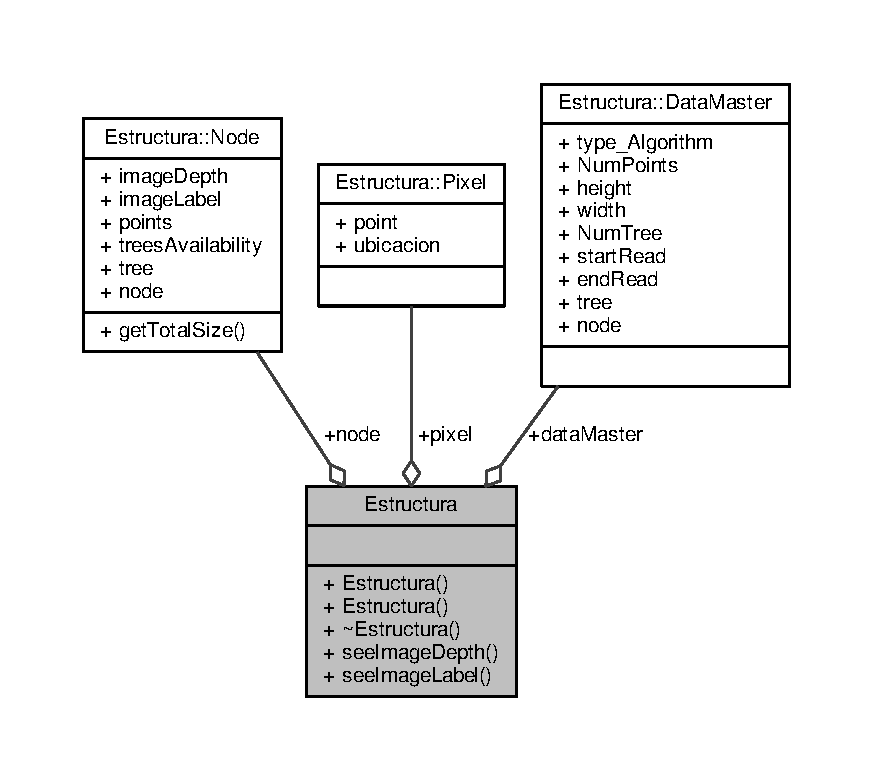
\includegraphics[width=350pt]{classEstructura__coll__graph}
\end{center}
\end{figure}
\subsection*{Classes}
\begin{DoxyCompactItemize}
\item 
struct \hyperlink{structEstructura_1_1DataMaster}{Data\+Master}
\item 
struct \hyperlink{structEstructura_1_1Node}{Node}
\item 
struct \hyperlink{structEstructura_1_1Pixel}{Pixel}
\end{DoxyCompactItemize}
\subsection*{Public Member Functions}
\begin{DoxyCompactItemize}
\item 
\hyperlink{classEstructura_a262933b2edef1ca54cff6ba1563fec6a}{Estructura} ()
\item 
\hyperlink{classEstructura_a03d6a9c7a66d9f71e8390fc7a928218a}{Estructura} (const \hyperlink{classEstructura}{Estructura} \&orig)
\item 
virtual \hyperlink{classEstructura_a03c32978a05236d51de8b8eb5875e2cd}{$\sim$\+Estructura} ()
\item 
void \hyperlink{classEstructura_a64b30b9326081ddd31ea330c4036cf5a}{see\+Image\+Depth} (int height, int width, cv\+::\+Mat image\+Depth)
\item 
void \hyperlink{classEstructura_a4d6f678e0c5a5f2df96b50064304eec1}{see\+Image\+Label} (cv\+::\+Mat \&image\+Label)
\end{DoxyCompactItemize}
\subsection*{Public Attributes}
\begin{DoxyCompactItemize}
\item 
struct \hyperlink{structEstructura_1_1Pixel}{Estructura\+::\+Pixel} \hyperlink{classEstructura_a654a8d1db30bd97916e083a4f7a05666}{pixel}
\item 
struct \hyperlink{structEstructura_1_1Node}{Estructura\+::\+Node} \hyperlink{classEstructura_a0b6ee5224146d9518cbfb9cc3cc6e8d9}{node}
\item 
struct \hyperlink{structEstructura_1_1DataMaster}{Estructura\+::\+Data\+Master} \hyperlink{classEstructura_ac594935213f660738514933d4a74f073}{data\+Master}
\end{DoxyCompactItemize}


\subsection{Constructor \& Destructor Documentation}
\index{Estructura@{Estructura}!Estructura@{Estructura}}
\index{Estructura@{Estructura}!Estructura@{Estructura}}
\subsubsection[{\texorpdfstring{Estructura()}{Estructura()}}]{\setlength{\rightskip}{0pt plus 5cm}Estructura\+::\+Estructura (
\begin{DoxyParamCaption}
{}
\end{DoxyParamCaption}
)}\hypertarget{classEstructura_a262933b2edef1ca54cff6ba1563fec6a}{}\label{classEstructura_a262933b2edef1ca54cff6ba1563fec6a}

\begin{DoxyCode}
17                        \{
18 \}
\end{DoxyCode}
\index{Estructura@{Estructura}!Estructura@{Estructura}}
\index{Estructura@{Estructura}!Estructura@{Estructura}}
\subsubsection[{\texorpdfstring{Estructura(const Estructura \&orig)}{Estructura(const Estructura &orig)}}]{\setlength{\rightskip}{0pt plus 5cm}Estructura\+::\+Estructura (
\begin{DoxyParamCaption}
\item[{const {\bf Estructura} \&}]{orig}
\end{DoxyParamCaption}
)}\hypertarget{classEstructura_a03d6a9c7a66d9f71e8390fc7a928218a}{}\label{classEstructura_a03d6a9c7a66d9f71e8390fc7a928218a}

\begin{DoxyCode}
20                                              \{
21 \}
\end{DoxyCode}
\index{Estructura@{Estructura}!````~Estructura@{$\sim$\+Estructura}}
\index{````~Estructura@{$\sim$\+Estructura}!Estructura@{Estructura}}
\subsubsection[{\texorpdfstring{$\sim$\+Estructura()}{~Estructura()}}]{\setlength{\rightskip}{0pt plus 5cm}Estructura\+::$\sim$\+Estructura (
\begin{DoxyParamCaption}
{}
\end{DoxyParamCaption}
)\hspace{0.3cm}{\ttfamily [virtual]}}\hypertarget{classEstructura_a03c32978a05236d51de8b8eb5875e2cd}{}\label{classEstructura_a03c32978a05236d51de8b8eb5875e2cd}

\begin{DoxyCode}
23                         \{
24 \}
\end{DoxyCode}


\subsection{Member Function Documentation}
\index{Estructura@{Estructura}!see\+Image\+Depth@{see\+Image\+Depth}}
\index{see\+Image\+Depth@{see\+Image\+Depth}!Estructura@{Estructura}}
\subsubsection[{\texorpdfstring{see\+Image\+Depth(int height, int width, cv\+::\+Mat image\+Depth)}{seeImageDepth(int height, int width, cv::Mat imageDepth)}}]{\setlength{\rightskip}{0pt plus 5cm}void Estructura\+::see\+Image\+Depth (
\begin{DoxyParamCaption}
\item[{int}]{height, }
\item[{int}]{width, }
\item[{cv\+::\+Mat}]{image\+Depth}
\end{DoxyParamCaption}
)}\hypertarget{classEstructura_a64b30b9326081ddd31ea330c4036cf5a}{}\label{classEstructura_a64b30b9326081ddd31ea330c4036cf5a}


Referenced by Image\+Manager\+::show\+Structure().


\begin{DoxyCode}
26                                                                      \{
27     cv::Mat depTem;
28     depTem = cv::Mat(height, width, CV\_16UC1, cv::Scalar(0));
29     
30     \textcolor{keywordtype}{int} mayor = 0;
31     \textcolor{keywordflow}{for} (\textcolor{keywordtype}{int} i = 0; i < height; i++) \{
32         \textcolor{keywordflow}{for} (\textcolor{keywordtype}{int} j = 0; j < width; j++) \{
33             cv::Scalar intensity = imageDepth.at<\textcolor{keywordtype}{unsigned} \textcolor{keywordtype}{short}>(i, j);
34             \textcolor{keywordflow}{if}(mayor < (\textcolor{keywordtype}{int}) intensity.val[0])\{
35                 mayor = intensity.val[0];
36             \}
37         \}
38     \}
39     
40     \textcolor{keywordflow}{for} (\textcolor{keywordtype}{int} i = 0; i < height; i++) \{
41         \textcolor{keywordflow}{for} (\textcolor{keywordtype}{int} j = 0; j < width; j++) \{
42             cv::Scalar intensity = imageDepth.at<\textcolor{keywordtype}{unsigned} \textcolor{keywordtype}{short}>(i, j);
43             \textcolor{keywordtype}{int} valor = intensity.val[0];
44             valor = ((255*valor)/mayor);
45             cv::Scalar temp = valor;
46             depTem.at<uchar>(i,j)= temp.val[0];     
47         \}
48     \}
49     cv::namedWindow( \textcolor{stringliteral}{"Original image"}, CV\_WINDOW\_AUTOSIZE ); 
50     cv::imshow( \textcolor{stringliteral}{"Original image"}, depTem ); 
51     cv::waitKey(2000);
52 \}
\end{DoxyCode}
\index{Estructura@{Estructura}!see\+Image\+Label@{see\+Image\+Label}}
\index{see\+Image\+Label@{see\+Image\+Label}!Estructura@{Estructura}}
\subsubsection[{\texorpdfstring{see\+Image\+Label(cv\+::\+Mat \&image\+Label)}{seeImageLabel(cv::Mat &imageLabel)}}]{\setlength{\rightskip}{0pt plus 5cm}void Estructura\+::see\+Image\+Label (
\begin{DoxyParamCaption}
\item[{cv\+::\+Mat \&}]{image\+Label}
\end{DoxyParamCaption}
)}\hypertarget{classEstructura_a4d6f678e0c5a5f2df96b50064304eec1}{}\label{classEstructura_a4d6f678e0c5a5f2df96b50064304eec1}


Referenced by Image\+Manager\+::show\+Structure().


\begin{DoxyCode}
54                                                \{
55     cv::namedWindow( \textcolor{stringliteral}{"Original image"}, CV\_WINDOW\_AUTOSIZE ); 
56     cv::imshow( \textcolor{stringliteral}{"Original image"}, imageLabel ); 
57     cv::waitKey(2000);
58 \}
\end{DoxyCode}


\subsection{Member Data Documentation}
\index{Estructura@{Estructura}!data\+Master@{data\+Master}}
\index{data\+Master@{data\+Master}!Estructura@{Estructura}}
\subsubsection[{\texorpdfstring{data\+Master}{dataMaster}}]{\setlength{\rightskip}{0pt plus 5cm}struct {\bf Estructura\+::\+Data\+Master}  Estructura\+::data\+Master}\hypertarget{classEstructura_ac594935213f660738514933d4a74f073}{}\label{classEstructura_ac594935213f660738514933d4a74f073}
\index{Estructura@{Estructura}!node@{node}}
\index{node@{node}!Estructura@{Estructura}}
\subsubsection[{\texorpdfstring{node}{node}}]{\setlength{\rightskip}{0pt plus 5cm}struct {\bf Estructura\+::\+Node}  Estructura\+::node}\hypertarget{classEstructura_a0b6ee5224146d9518cbfb9cc3cc6e8d9}{}\label{classEstructura_a0b6ee5224146d9518cbfb9cc3cc6e8d9}


Referenced by Estructura\+::\+Node\+::get\+Total\+Size().

\index{Estructura@{Estructura}!pixel@{pixel}}
\index{pixel@{pixel}!Estructura@{Estructura}}
\subsubsection[{\texorpdfstring{pixel}{pixel}}]{\setlength{\rightskip}{0pt plus 5cm}struct {\bf Estructura\+::\+Pixel}  Estructura\+::pixel}\hypertarget{classEstructura_a654a8d1db30bd97916e083a4f7a05666}{}\label{classEstructura_a654a8d1db30bd97916e083a4f7a05666}


The documentation for this class was generated from the following files\+:\begin{DoxyCompactItemize}
\item 
\hyperlink{Estructura_8h}{Estructura.\+h}\item 
\hyperlink{Estructura_8cpp}{Estructura.\+cpp}\end{DoxyCompactItemize}

\hypertarget{classrdf_1_1bpc_1_1Features}{}\section{rdf\+:\+:bpc\+:\+:Features Class Reference}
\label{classrdf_1_1bpc_1_1Features}\index{rdf\+::bpc\+::\+Features@{rdf\+::bpc\+::\+Features}}


{\ttfamily \#include $<$Features.\+h$>$}



Collaboration diagram for rdf\+:\+:bpc\+:\+:Features\+:
\nopagebreak
\begin{figure}[H]
\begin{center}
\leavevmode
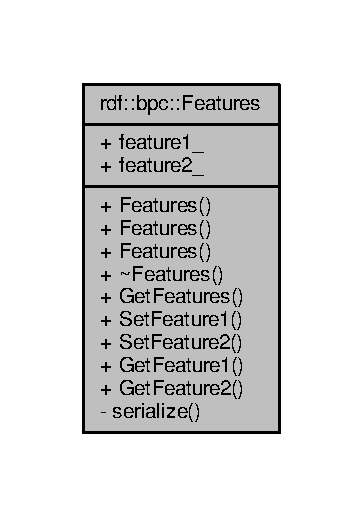
\includegraphics[width=174pt]{classrdf_1_1bpc_1_1Features__coll__graph}
\end{center}
\end{figure}
\subsection*{Public Member Functions}
\begin{DoxyCompactItemize}
\item 
\hyperlink{classrdf_1_1bpc_1_1Features_abfca82d68cea9e637d0b601395d6da6f}{Features} ()
\item 
\hyperlink{classrdf_1_1bpc_1_1Features_a47d8976ae88c7c3dc1445d1437eba66c}{Features} (float, float, float, float)
\item 
\hyperlink{classrdf_1_1bpc_1_1Features_a9055f349ed663508478dbe1e92dcdceb}{Features} (const \hyperlink{classrdf_1_1bpc_1_1Features}{Features} \&orig)
\item 
virtual \hyperlink{classrdf_1_1bpc_1_1Features_a24752e0df868197b2225abc369a374e7}{$\sim$\+Features} ()
\item 
std\+::pair$<$ \hyperlink{namespacerdf_1_1bpc_a507d4ac6b23164245625d13196e564bc}{Feature}, \hyperlink{namespacerdf_1_1bpc_a507d4ac6b23164245625d13196e564bc}{Feature} $>$ \hyperlink{classrdf_1_1bpc_1_1Features_aadc3584d493974a48a3ec633eb49bbda}{Get\+Features} ()
\item 
\hyperlink{namespacerdf_1_1bpc_a507d4ac6b23164245625d13196e564bc}{Feature} \hyperlink{classrdf_1_1bpc_1_1Features_add4c2edfb1f05b59662e9f2ebafafdd2}{Set\+Feature1} (float x, float y)
\item 
\hyperlink{namespacerdf_1_1bpc_a507d4ac6b23164245625d13196e564bc}{Feature} \hyperlink{classrdf_1_1bpc_1_1Features_a0091e0dd9ba651e146a12562e8ecaa0e}{Set\+Feature2} (float x, float y)
\item 
\hyperlink{namespacerdf_1_1bpc_a507d4ac6b23164245625d13196e564bc}{Feature} \hyperlink{classrdf_1_1bpc_1_1Features_a2e893eccf388415169cd08b45d9d1964}{Get\+Feature1} ()
\item 
\hyperlink{namespacerdf_1_1bpc_a507d4ac6b23164245625d13196e564bc}{Feature} \hyperlink{classrdf_1_1bpc_1_1Features_a4a9aae0520825d9f9bee370449632522}{Get\+Feature2} ()
\end{DoxyCompactItemize}
\subsection*{Public Attributes}
\begin{DoxyCompactItemize}
\item 
\hyperlink{namespacerdf_1_1bpc_a507d4ac6b23164245625d13196e564bc}{Feature} \hyperlink{classrdf_1_1bpc_1_1Features_a01f4d6cb79311da3b39f82882112bbcb}{feature1\+\_\+}
\item 
\hyperlink{namespacerdf_1_1bpc_a507d4ac6b23164245625d13196e564bc}{Feature} \hyperlink{classrdf_1_1bpc_1_1Features_a563e43877615b6967a5ec9049bab4b65}{feature2\+\_\+}
\end{DoxyCompactItemize}
\subsection*{Private Member Functions}
\begin{DoxyCompactItemize}
\item 
{\footnotesize template$<$class Archive $>$ }\\void \hyperlink{classrdf_1_1bpc_1_1Features_abd95abc6646db661d105c9bb0317ad7f}{serialize} (Archive \&ar, const unsigned int version)
\end{DoxyCompactItemize}
\subsection*{Friends}
\begin{DoxyCompactItemize}
\item 
class \hyperlink{classrdf_1_1bpc_1_1Features_ac98d07dd8f7b70e16ccb9a01abf56b9c}{boost\+::serialization\+::access}
\end{DoxyCompactItemize}


\subsection{Constructor \& Destructor Documentation}
\index{rdf\+::bpc\+::\+Features@{rdf\+::bpc\+::\+Features}!Features@{Features}}
\index{Features@{Features}!rdf\+::bpc\+::\+Features@{rdf\+::bpc\+::\+Features}}
\subsubsection[{\texorpdfstring{Features()}{Features()}}]{\setlength{\rightskip}{0pt plus 5cm}Features\+::\+Features (
\begin{DoxyParamCaption}
{}
\end{DoxyParamCaption}
)}\hypertarget{classrdf_1_1bpc_1_1Features_abfca82d68cea9e637d0b601395d6da6f}{}\label{classrdf_1_1bpc_1_1Features_abfca82d68cea9e637d0b601395d6da6f}


References feature1\+\_\+, and feature2\+\_\+.


\begin{DoxyCode}
30                    \{
31   \hyperlink{classrdf_1_1bpc_1_1Features_a01f4d6cb79311da3b39f82882112bbcb}{feature1\_}.x = 0;
32   \hyperlink{classrdf_1_1bpc_1_1Features_a01f4d6cb79311da3b39f82882112bbcb}{feature1\_}.y = 0;
33   \hyperlink{classrdf_1_1bpc_1_1Features_a563e43877615b6967a5ec9049bab4b65}{feature2\_}.x = 0;
34   \hyperlink{classrdf_1_1bpc_1_1Features_a563e43877615b6967a5ec9049bab4b65}{feature2\_}.y = 0;
35 \}
\end{DoxyCode}
\index{rdf\+::bpc\+::\+Features@{rdf\+::bpc\+::\+Features}!Features@{Features}}
\index{Features@{Features}!rdf\+::bpc\+::\+Features@{rdf\+::bpc\+::\+Features}}
\subsubsection[{\texorpdfstring{Features(float, float, float, float)}{Features(float, float, float, float)}}]{\setlength{\rightskip}{0pt plus 5cm}Features\+::\+Features (
\begin{DoxyParamCaption}
\item[{float}]{feat1\+\_\+x, }
\item[{float}]{feat1\+\_\+y, }
\item[{float}]{feat2\+\_\+x, }
\item[{float}]{feat2\+\_\+y}
\end{DoxyParamCaption}
)}\hypertarget{classrdf_1_1bpc_1_1Features_a47d8976ae88c7c3dc1445d1437eba66c}{}\label{classrdf_1_1bpc_1_1Features_a47d8976ae88c7c3dc1445d1437eba66c}


References feature1\+\_\+, and feature2\+\_\+.


\begin{DoxyCode}
37                                                                              \{
38   \hyperlink{classrdf_1_1bpc_1_1Features_a01f4d6cb79311da3b39f82882112bbcb}{feature1\_}.x = feat1\_x;
39   \hyperlink{classrdf_1_1bpc_1_1Features_a01f4d6cb79311da3b39f82882112bbcb}{feature1\_}.y = feat1\_y;
40   \hyperlink{classrdf_1_1bpc_1_1Features_a563e43877615b6967a5ec9049bab4b65}{feature2\_}.x = feat2\_x;
41   \hyperlink{classrdf_1_1bpc_1_1Features_a563e43877615b6967a5ec9049bab4b65}{feature2\_}.y = feat2\_y;
42 \}
\end{DoxyCode}
\index{rdf\+::bpc\+::\+Features@{rdf\+::bpc\+::\+Features}!Features@{Features}}
\index{Features@{Features}!rdf\+::bpc\+::\+Features@{rdf\+::bpc\+::\+Features}}
\subsubsection[{\texorpdfstring{Features(const Features \&orig)}{Features(const Features &orig)}}]{\setlength{\rightskip}{0pt plus 5cm}Features\+::\+Features (
\begin{DoxyParamCaption}
\item[{const {\bf Features} \&}]{orig}
\end{DoxyParamCaption}
)}\hypertarget{classrdf_1_1bpc_1_1Features_a9055f349ed663508478dbe1e92dcdceb}{}\label{classrdf_1_1bpc_1_1Features_a9055f349ed663508478dbe1e92dcdceb}


References feature1\+\_\+, and feature2\+\_\+.


\begin{DoxyCode}
65                                        \{
66   \hyperlink{classrdf_1_1bpc_1_1Features_a01f4d6cb79311da3b39f82882112bbcb}{feature1\_} = orig.\hyperlink{classrdf_1_1bpc_1_1Features_a01f4d6cb79311da3b39f82882112bbcb}{feature1\_};
67   \hyperlink{classrdf_1_1bpc_1_1Features_a563e43877615b6967a5ec9049bab4b65}{feature2\_} = orig.\hyperlink{classrdf_1_1bpc_1_1Features_a563e43877615b6967a5ec9049bab4b65}{feature2\_};
68 \}
\end{DoxyCode}
\index{rdf\+::bpc\+::\+Features@{rdf\+::bpc\+::\+Features}!````~Features@{$\sim$\+Features}}
\index{````~Features@{$\sim$\+Features}!rdf\+::bpc\+::\+Features@{rdf\+::bpc\+::\+Features}}
\subsubsection[{\texorpdfstring{$\sim$\+Features()}{~Features()}}]{\setlength{\rightskip}{0pt plus 5cm}Features\+::$\sim$\+Features (
\begin{DoxyParamCaption}
{}
\end{DoxyParamCaption}
)\hspace{0.3cm}{\ttfamily [virtual]}}\hypertarget{classrdf_1_1bpc_1_1Features_a24752e0df868197b2225abc369a374e7}{}\label{classrdf_1_1bpc_1_1Features_a24752e0df868197b2225abc369a374e7}

\begin{DoxyCode}
70                     \{
71 \}
\end{DoxyCode}


\subsection{Member Function Documentation}
\index{rdf\+::bpc\+::\+Features@{rdf\+::bpc\+::\+Features}!Get\+Feature1@{Get\+Feature1}}
\index{Get\+Feature1@{Get\+Feature1}!rdf\+::bpc\+::\+Features@{rdf\+::bpc\+::\+Features}}
\subsubsection[{\texorpdfstring{Get\+Feature1()}{GetFeature1()}}]{\setlength{\rightskip}{0pt plus 5cm}{\bf Feature} Features\+::\+Get\+Feature1 (
\begin{DoxyParamCaption}
{}
\end{DoxyParamCaption}
)}\hypertarget{classrdf_1_1bpc_1_1Features_a2e893eccf388415169cd08b45d9d1964}{}\label{classrdf_1_1bpc_1_1Features_a2e893eccf388415169cd08b45d9d1964}


References feature1\+\_\+.



Referenced by rdf\+::bpc\+::\+Features\+Mat\+::\+Print().


\begin{DoxyCode}
57                              \{
58   \textcolor{keywordflow}{return} \hyperlink{classrdf_1_1bpc_1_1Features_a01f4d6cb79311da3b39f82882112bbcb}{feature1\_};
59 \}
\end{DoxyCode}
\index{rdf\+::bpc\+::\+Features@{rdf\+::bpc\+::\+Features}!Get\+Feature2@{Get\+Feature2}}
\index{Get\+Feature2@{Get\+Feature2}!rdf\+::bpc\+::\+Features@{rdf\+::bpc\+::\+Features}}
\subsubsection[{\texorpdfstring{Get\+Feature2()}{GetFeature2()}}]{\setlength{\rightskip}{0pt plus 5cm}{\bf Feature} Features\+::\+Get\+Feature2 (
\begin{DoxyParamCaption}
{}
\end{DoxyParamCaption}
)}\hypertarget{classrdf_1_1bpc_1_1Features_a4a9aae0520825d9f9bee370449632522}{}\label{classrdf_1_1bpc_1_1Features_a4a9aae0520825d9f9bee370449632522}


References feature2\+\_\+.



Referenced by rdf\+::bpc\+::\+Features\+Mat\+::\+Print().


\begin{DoxyCode}
61                              \{
62   \textcolor{keywordflow}{return} \hyperlink{classrdf_1_1bpc_1_1Features_a563e43877615b6967a5ec9049bab4b65}{feature2\_};
63 \}
\end{DoxyCode}
\index{rdf\+::bpc\+::\+Features@{rdf\+::bpc\+::\+Features}!Get\+Features@{Get\+Features}}
\index{Get\+Features@{Get\+Features}!rdf\+::bpc\+::\+Features@{rdf\+::bpc\+::\+Features}}
\subsubsection[{\texorpdfstring{Get\+Features()}{GetFeatures()}}]{\setlength{\rightskip}{0pt plus 5cm}std\+::pair$<${\bf Feature}, {\bf Feature}$>$ rdf\+::bpc\+::\+Features\+::\+Get\+Features (
\begin{DoxyParamCaption}
{}
\end{DoxyParamCaption}
)\hspace{0.3cm}{\ttfamily [inline]}}\hypertarget{classrdf_1_1bpc_1_1Features_aadc3584d493974a48a3ec633eb49bbda}{}\label{classrdf_1_1bpc_1_1Features_aadc3584d493974a48a3ec633eb49bbda}


References feature1\+\_\+.


\begin{DoxyCode}
48 \{\}; \textcolor{comment}{//TODO}
\end{DoxyCode}
\index{rdf\+::bpc\+::\+Features@{rdf\+::bpc\+::\+Features}!serialize@{serialize}}
\index{serialize@{serialize}!rdf\+::bpc\+::\+Features@{rdf\+::bpc\+::\+Features}}
\subsubsection[{\texorpdfstring{serialize(\+Archive \&ar, const unsigned int version)}{serialize(Archive &ar, const unsigned int version)}}]{\setlength{\rightskip}{0pt plus 5cm}template$<$class Archive $>$ void rdf\+::bpc\+::\+Features\+::serialize (
\begin{DoxyParamCaption}
\item[{Archive \&}]{ar, }
\item[{const unsigned int}]{version}
\end{DoxyParamCaption}
)\hspace{0.3cm}{\ttfamily [inline]}, {\ttfamily [private]}}\hypertarget{classrdf_1_1bpc_1_1Features_abd95abc6646db661d105c9bb0317ad7f}{}\label{classrdf_1_1bpc_1_1Features_abd95abc6646db661d105c9bb0317ad7f}

\begin{DoxyCode}
63           \{
64             ar & \hyperlink{classrdf_1_1bpc_1_1Features_a01f4d6cb79311da3b39f82882112bbcb}{feature1\_}.x;
65             ar & \hyperlink{classrdf_1_1bpc_1_1Features_a01f4d6cb79311da3b39f82882112bbcb}{feature1\_}.y;
66             ar & \hyperlink{classrdf_1_1bpc_1_1Features_a563e43877615b6967a5ec9049bab4b65}{feature2\_}.x;
67             ar & \hyperlink{classrdf_1_1bpc_1_1Features_a563e43877615b6967a5ec9049bab4b65}{feature2\_}.y;
68           \}
\end{DoxyCode}
\index{rdf\+::bpc\+::\+Features@{rdf\+::bpc\+::\+Features}!Set\+Feature1@{Set\+Feature1}}
\index{Set\+Feature1@{Set\+Feature1}!rdf\+::bpc\+::\+Features@{rdf\+::bpc\+::\+Features}}
\subsubsection[{\texorpdfstring{Set\+Feature1(float x, float y)}{SetFeature1(float x, float y)}}]{\setlength{\rightskip}{0pt plus 5cm}{\bf Feature} Features\+::\+Set\+Feature1 (
\begin{DoxyParamCaption}
\item[{float}]{x, }
\item[{float}]{y}
\end{DoxyParamCaption}
)}\hypertarget{classrdf_1_1bpc_1_1Features_add4c2edfb1f05b59662e9f2ebafafdd2}{}\label{classrdf_1_1bpc_1_1Features_add4c2edfb1f05b59662e9f2ebafafdd2}


References feature1\+\_\+.



Referenced by rdf\+::bpc\+::\+Features\+Mat\+::\+Generate\+Features\+Vector().


\begin{DoxyCode}
45                                              \{
46   \hyperlink{classrdf_1_1bpc_1_1Features_a01f4d6cb79311da3b39f82882112bbcb}{feature1\_}.x = x;
47   \hyperlink{classrdf_1_1bpc_1_1Features_a01f4d6cb79311da3b39f82882112bbcb}{feature1\_}.y = y;
48   \textcolor{keywordflow}{return} \hyperlink{classrdf_1_1bpc_1_1Features_a01f4d6cb79311da3b39f82882112bbcb}{feature1\_};
49 \}
\end{DoxyCode}
\index{rdf\+::bpc\+::\+Features@{rdf\+::bpc\+::\+Features}!Set\+Feature2@{Set\+Feature2}}
\index{Set\+Feature2@{Set\+Feature2}!rdf\+::bpc\+::\+Features@{rdf\+::bpc\+::\+Features}}
\subsubsection[{\texorpdfstring{Set\+Feature2(float x, float y)}{SetFeature2(float x, float y)}}]{\setlength{\rightskip}{0pt plus 5cm}{\bf Feature} Features\+::\+Set\+Feature2 (
\begin{DoxyParamCaption}
\item[{float}]{x, }
\item[{float}]{y}
\end{DoxyParamCaption}
)}\hypertarget{classrdf_1_1bpc_1_1Features_a0091e0dd9ba651e146a12562e8ecaa0e}{}\label{classrdf_1_1bpc_1_1Features_a0091e0dd9ba651e146a12562e8ecaa0e}


References feature2\+\_\+.



Referenced by rdf\+::bpc\+::\+Features\+Mat\+::\+Generate\+Features\+Vector().


\begin{DoxyCode}
51                                              \{
52   \hyperlink{classrdf_1_1bpc_1_1Features_a563e43877615b6967a5ec9049bab4b65}{feature2\_}.x = x;
53   \hyperlink{classrdf_1_1bpc_1_1Features_a563e43877615b6967a5ec9049bab4b65}{feature2\_}.y = y;
54   \textcolor{keywordflow}{return} \hyperlink{classrdf_1_1bpc_1_1Features_a563e43877615b6967a5ec9049bab4b65}{feature2\_};
55 \}
\end{DoxyCode}


\subsection{Friends And Related Function Documentation}
\index{rdf\+::bpc\+::\+Features@{rdf\+::bpc\+::\+Features}!boost\+::serialization\+::access@{boost\+::serialization\+::access}}
\index{boost\+::serialization\+::access@{boost\+::serialization\+::access}!rdf\+::bpc\+::\+Features@{rdf\+::bpc\+::\+Features}}
\subsubsection[{\texorpdfstring{boost\+::serialization\+::access}{boost::serialization::access}}]{\setlength{\rightskip}{0pt plus 5cm}friend class boost\+::serialization\+::access\hspace{0.3cm}{\ttfamily [friend]}}\hypertarget{classrdf_1_1bpc_1_1Features_ac98d07dd8f7b70e16ccb9a01abf56b9c}{}\label{classrdf_1_1bpc_1_1Features_ac98d07dd8f7b70e16ccb9a01abf56b9c}


\subsection{Member Data Documentation}
\index{rdf\+::bpc\+::\+Features@{rdf\+::bpc\+::\+Features}!feature1\+\_\+@{feature1\+\_\+}}
\index{feature1\+\_\+@{feature1\+\_\+}!rdf\+::bpc\+::\+Features@{rdf\+::bpc\+::\+Features}}
\subsubsection[{\texorpdfstring{feature1\+\_\+}{feature1_}}]{\setlength{\rightskip}{0pt plus 5cm}{\bf Feature} rdf\+::bpc\+::\+Features\+::feature1\+\_\+}\hypertarget{classrdf_1_1bpc_1_1Features_a01f4d6cb79311da3b39f82882112bbcb}{}\label{classrdf_1_1bpc_1_1Features_a01f4d6cb79311da3b39f82882112bbcb}


Referenced by Features(), Get\+Feature1(), Get\+Features(), rdf\+::\+Node\+Result\+::reduce(), and Set\+Feature1().

\index{rdf\+::bpc\+::\+Features@{rdf\+::bpc\+::\+Features}!feature2\+\_\+@{feature2\+\_\+}}
\index{feature2\+\_\+@{feature2\+\_\+}!rdf\+::bpc\+::\+Features@{rdf\+::bpc\+::\+Features}}
\subsubsection[{\texorpdfstring{feature2\+\_\+}{feature2_}}]{\setlength{\rightskip}{0pt plus 5cm}{\bf Feature} rdf\+::bpc\+::\+Features\+::feature2\+\_\+}\hypertarget{classrdf_1_1bpc_1_1Features_a563e43877615b6967a5ec9049bab4b65}{}\label{classrdf_1_1bpc_1_1Features_a563e43877615b6967a5ec9049bab4b65}


Referenced by Features(), Get\+Feature2(), rdf\+::\+Node\+Result\+::reduce(), and Set\+Feature2().



The documentation for this class was generated from the following files\+:\begin{DoxyCompactItemize}
\item 
\hyperlink{Features_8h}{Features.\+h}\item 
\hyperlink{Features_8cpp}{Features.\+cpp}\end{DoxyCompactItemize}

\hypertarget{classrdf_1_1bpc_1_1FeaturesMat}{}\section{rdf\+:\+:bpc\+:\+:Features\+Mat Class Reference}
\label{classrdf_1_1bpc_1_1FeaturesMat}\index{rdf\+::bpc\+::\+Features\+Mat@{rdf\+::bpc\+::\+Features\+Mat}}


{\ttfamily \#include $<$Features\+Mat.\+h$>$}



Collaboration diagram for rdf\+:\+:bpc\+:\+:Features\+Mat\+:
\nopagebreak
\begin{figure}[H]
\begin{center}
\leavevmode
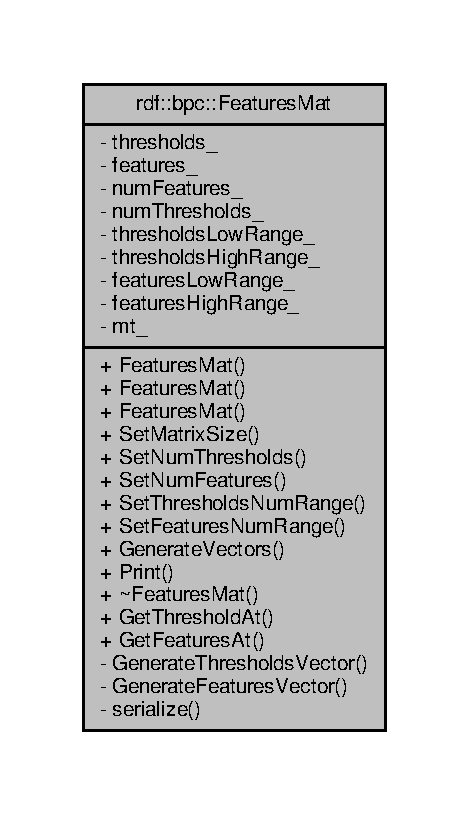
\includegraphics[width=225pt]{classrdf_1_1bpc_1_1FeaturesMat__coll__graph}
\end{center}
\end{figure}
\subsection*{Public Member Functions}
\begin{DoxyCompactItemize}
\item 
\hyperlink{classrdf_1_1bpc_1_1FeaturesMat_a97d121d34349bf2c59b94c2048cf8543}{Features\+Mat} ()
\item 
\hyperlink{classrdf_1_1bpc_1_1FeaturesMat_abc3e95ccbc49b66cd506496985ca8fb0}{Features\+Mat} (const \hyperlink{classrdf_1_1bpc_1_1FeaturesMat}{Features\+Mat} \&orig)
\item 
\hyperlink{classrdf_1_1bpc_1_1FeaturesMat_a4656343c72c85949ef2e13d01f4b0bbf}{Features\+Mat} (int fn, float fh, float fl, int tn, float th, float tl)
\item 
void \hyperlink{classrdf_1_1bpc_1_1FeaturesMat_a14292e637f99011c2f519f938acf89c6}{Set\+Matrix\+Size} (int x, int y)
\item 
void \hyperlink{classrdf_1_1bpc_1_1FeaturesMat_a4d975d667769356abb6ef91a379fbe38}{Set\+Num\+Thresholds} (int)
\item 
void \hyperlink{classrdf_1_1bpc_1_1FeaturesMat_abb8b176b7082837f435b66e79802114d}{Set\+Num\+Features} (int)
\item 
void \hyperlink{classrdf_1_1bpc_1_1FeaturesMat_a03f0951ab28c3f8056eafb5c76412519}{Set\+Thresholds\+Num\+Range} (float high, float low)
\item 
void \hyperlink{classrdf_1_1bpc_1_1FeaturesMat_a46e93bc1f4714aa57bee42d7e1da35fd}{Set\+Features\+Num\+Range} (float high, float low)
\item 
void \hyperlink{classrdf_1_1bpc_1_1FeaturesMat_aafcb6a653e6f4e161ca91b22710ff226}{Generate\+Vectors} ()
\item 
void \hyperlink{classrdf_1_1bpc_1_1FeaturesMat_a1c8094aad67feee40dfb71d325310e98}{Print} ()
\item 
virtual \hyperlink{classrdf_1_1bpc_1_1FeaturesMat_a5e01733c2446354d4dea3b149d74ce2a}{$\sim$\+Features\+Mat} ()
\item 
float \hyperlink{classrdf_1_1bpc_1_1FeaturesMat_a254007ddad6b1c1f1f91582b69a1957c}{Get\+Threshold\+At} (int x)
\item 
\hyperlink{classrdf_1_1bpc_1_1Features}{Features} \hyperlink{classrdf_1_1bpc_1_1FeaturesMat_a98330606d445ea0a8733ee308756e42f}{Get\+Features\+At} (int x)
\end{DoxyCompactItemize}
\subsection*{Private Member Functions}
\begin{DoxyCompactItemize}
\item 
void \hyperlink{classrdf_1_1bpc_1_1FeaturesMat_a58963a1543309ade81bb5aeaf2508e14}{Generate\+Thresholds\+Vector} ()
\item 
void \hyperlink{classrdf_1_1bpc_1_1FeaturesMat_a53eb814797bbd35eedc0d98cedcb4952}{Generate\+Features\+Vector} ()
\item 
{\footnotesize template$<$class Archive $>$ }\\void \hyperlink{classrdf_1_1bpc_1_1FeaturesMat_ad1dcd821565ad3a3dea0dd5953e6f678}{serialize} (Archive \&ar, const unsigned int version)
\end{DoxyCompactItemize}
\subsection*{Private Attributes}
\begin{DoxyCompactItemize}
\item 
std\+::vector$<$ float $>$ \hyperlink{classrdf_1_1bpc_1_1FeaturesMat_af78d3fa0ca76bc3ec1102772fcbac819}{thresholds\+\_\+}
\item 
std\+::vector$<$ \hyperlink{classrdf_1_1bpc_1_1Features}{Features} $>$ \hyperlink{classrdf_1_1bpc_1_1FeaturesMat_a476cd5bf74e3808ea56e585db0083ceb}{features\+\_\+}
\item 
int \hyperlink{classrdf_1_1bpc_1_1FeaturesMat_acc84dd8b048451bbe7be60dce7c3417c}{num\+Features\+\_\+}
\item 
int \hyperlink{classrdf_1_1bpc_1_1FeaturesMat_aeb9a1a867455c3bb26292ff63fe6aada}{num\+Thresholds\+\_\+}
\item 
float \hyperlink{classrdf_1_1bpc_1_1FeaturesMat_a9b44bbd98c5850168c4c33054d6e5ed2}{thresholds\+Low\+Range\+\_\+}
\item 
float \hyperlink{classrdf_1_1bpc_1_1FeaturesMat_a0458cdc2eafc76455938ab3d54fcb762}{thresholds\+High\+Range\+\_\+}
\item 
float \hyperlink{classrdf_1_1bpc_1_1FeaturesMat_a77e4d847ce04f626964fe361d7bee1a5}{features\+Low\+Range\+\_\+}
\item 
float \hyperlink{classrdf_1_1bpc_1_1FeaturesMat_a3c6a55c571fac002562a59b67f681719}{features\+High\+Range\+\_\+}
\end{DoxyCompactItemize}
\subsection*{Static Private Attributes}
\begin{DoxyCompactItemize}
\item 
static std\+::mt19937 \hyperlink{classrdf_1_1bpc_1_1FeaturesMat_ae4222f4a5e1a75b6bacd6f03108a2095}{mt\+\_\+} = \hyperlink{FeaturesMat_8cpp_a0c2f708dd4e06898c274c468e8f281c2}{Initialize\+Random\+Device}()
\end{DoxyCompactItemize}
\subsection*{Friends}
\begin{DoxyCompactItemize}
\item 
{\footnotesize template$<$class T $>$ }\\class \hyperlink{classrdf_1_1bpc_1_1FeaturesMat_a6216d6f816a4e3b1567b5b11487815d8}{Matrix}
\item 
class \hyperlink{classrdf_1_1bpc_1_1FeaturesMat_ac98d07dd8f7b70e16ccb9a01abf56b9c}{boost\+::serialization\+::access}
\end{DoxyCompactItemize}


\subsection{Constructor \& Destructor Documentation}
\index{rdf\+::bpc\+::\+Features\+Mat@{rdf\+::bpc\+::\+Features\+Mat}!Features\+Mat@{Features\+Mat}}
\index{Features\+Mat@{Features\+Mat}!rdf\+::bpc\+::\+Features\+Mat@{rdf\+::bpc\+::\+Features\+Mat}}
\subsubsection[{\texorpdfstring{Features\+Mat()}{FeaturesMat()}}]{\setlength{\rightskip}{0pt plus 5cm}Features\+Mat\+::\+Features\+Mat (
\begin{DoxyParamCaption}
{}
\end{DoxyParamCaption}
)}\hypertarget{classrdf_1_1bpc_1_1FeaturesMat_a97d121d34349bf2c59b94c2048cf8543}{}\label{classrdf_1_1bpc_1_1FeaturesMat_a97d121d34349bf2c59b94c2048cf8543}

\begin{DoxyCode}
30                          \{
31   \hyperlink{classrdf_1_1bpc_1_1FeaturesMat_a9b44bbd98c5850168c4c33054d6e5ed2}{thresholdsLowRange\_} = 0;
32   \hyperlink{classrdf_1_1bpc_1_1FeaturesMat_a0458cdc2eafc76455938ab3d54fcb762}{thresholdsHighRange\_} = 0;
33   \hyperlink{classrdf_1_1bpc_1_1FeaturesMat_a77e4d847ce04f626964fe361d7bee1a5}{featuresLowRange\_} = 0;
34   \hyperlink{classrdf_1_1bpc_1_1FeaturesMat_a3c6a55c571fac002562a59b67f681719}{featuresHighRange\_} = 0;
35   \hyperlink{classrdf_1_1bpc_1_1FeaturesMat_acc84dd8b048451bbe7be60dce7c3417c}{numFeatures\_} = 0;
36   \hyperlink{classrdf_1_1bpc_1_1FeaturesMat_aeb9a1a867455c3bb26292ff63fe6aada}{numThresholds\_} = 0;
37 \}
\end{DoxyCode}
\index{rdf\+::bpc\+::\+Features\+Mat@{rdf\+::bpc\+::\+Features\+Mat}!Features\+Mat@{Features\+Mat}}
\index{Features\+Mat@{Features\+Mat}!rdf\+::bpc\+::\+Features\+Mat@{rdf\+::bpc\+::\+Features\+Mat}}
\subsubsection[{\texorpdfstring{Features\+Mat(const Features\+Mat \&orig)}{FeaturesMat(const FeaturesMat &orig)}}]{\setlength{\rightskip}{0pt plus 5cm}Features\+Mat\+::\+Features\+Mat (
\begin{DoxyParamCaption}
\item[{const {\bf Features\+Mat} \&}]{orig}
\end{DoxyParamCaption}
)}\hypertarget{classrdf_1_1bpc_1_1FeaturesMat_abc3e95ccbc49b66cd506496985ca8fb0}{}\label{classrdf_1_1bpc_1_1FeaturesMat_abc3e95ccbc49b66cd506496985ca8fb0}


References features\+\_\+, num\+Features\+\_\+, num\+Thresholds\+\_\+, and thresholds\+\_\+.


\begin{DoxyCode}
47                                                 \{
48   \hyperlink{classrdf_1_1bpc_1_1FeaturesMat_a14292e637f99011c2f519f938acf89c6}{SetMatrixSize}( orig.\hyperlink{classrdf_1_1bpc_1_1FeaturesMat_acc84dd8b048451bbe7be60dce7c3417c}{numFeatures\_}, orig.\hyperlink{classrdf_1_1bpc_1_1FeaturesMat_aeb9a1a867455c3bb26292ff63fe6aada}{numThresholds\_});
49   \hyperlink{classrdf_1_1bpc_1_1FeaturesMat_af78d3fa0ca76bc3ec1102772fcbac819}{thresholds\_} =  orig.\hyperlink{classrdf_1_1bpc_1_1FeaturesMat_af78d3fa0ca76bc3ec1102772fcbac819}{thresholds\_};
50   \hyperlink{classrdf_1_1bpc_1_1FeaturesMat_a476cd5bf74e3808ea56e585db0083ceb}{features\_}=  orig.\hyperlink{classrdf_1_1bpc_1_1FeaturesMat_a476cd5bf74e3808ea56e585db0083ceb}{features\_};
51 \}
\end{DoxyCode}
\index{rdf\+::bpc\+::\+Features\+Mat@{rdf\+::bpc\+::\+Features\+Mat}!Features\+Mat@{Features\+Mat}}
\index{Features\+Mat@{Features\+Mat}!rdf\+::bpc\+::\+Features\+Mat@{rdf\+::bpc\+::\+Features\+Mat}}
\subsubsection[{\texorpdfstring{Features\+Mat(int fn, float fh, float fl, int tn, float th, float tl)}{FeaturesMat(int fn, float fh, float fl, int tn, float th, float tl)}}]{\setlength{\rightskip}{0pt plus 5cm}Features\+Mat\+::\+Features\+Mat (
\begin{DoxyParamCaption}
\item[{int}]{fn, }
\item[{float}]{fh, }
\item[{float}]{fl, }
\item[{int}]{tn, }
\item[{float}]{th, }
\item[{float}]{tl}
\end{DoxyParamCaption}
)}\hypertarget{classrdf_1_1bpc_1_1FeaturesMat_a4656343c72c85949ef2e13d01f4b0bbf}{}\label{classrdf_1_1bpc_1_1FeaturesMat_a4656343c72c85949ef2e13d01f4b0bbf}

\begin{DoxyCode}
40                                                                                          \{
41 
42     \hyperlink{classrdf_1_1bpc_1_1FeaturesMat_a14292e637f99011c2f519f938acf89c6}{SetMatrixSize}(numFeatures, numThresholds);
43     \hyperlink{classrdf_1_1bpc_1_1FeaturesMat_a03f0951ab28c3f8056eafb5c76412519}{SetThresholdsNumRange}(thresholdsHigh,thresholdsLow);
44     \hyperlink{classrdf_1_1bpc_1_1FeaturesMat_a46e93bc1f4714aa57bee42d7e1da35fd}{SetFeaturesNumRange}(featuresHigh, featuresLow);
45 \}
\end{DoxyCode}
\index{rdf\+::bpc\+::\+Features\+Mat@{rdf\+::bpc\+::\+Features\+Mat}!````~Features\+Mat@{$\sim$\+Features\+Mat}}
\index{````~Features\+Mat@{$\sim$\+Features\+Mat}!rdf\+::bpc\+::\+Features\+Mat@{rdf\+::bpc\+::\+Features\+Mat}}
\subsubsection[{\texorpdfstring{$\sim$\+Features\+Mat()}{~FeaturesMat()}}]{\setlength{\rightskip}{0pt plus 5cm}Features\+Mat\+::$\sim$\+Features\+Mat (
\begin{DoxyParamCaption}
{}
\end{DoxyParamCaption}
)\hspace{0.3cm}{\ttfamily [virtual]}}\hypertarget{classrdf_1_1bpc_1_1FeaturesMat_a5e01733c2446354d4dea3b149d74ce2a}{}\label{classrdf_1_1bpc_1_1FeaturesMat_a5e01733c2446354d4dea3b149d74ce2a}

\begin{DoxyCode}
53                           \{
54 
55 \}
\end{DoxyCode}


\subsection{Member Function Documentation}
\index{rdf\+::bpc\+::\+Features\+Mat@{rdf\+::bpc\+::\+Features\+Mat}!Generate\+Features\+Vector@{Generate\+Features\+Vector}}
\index{Generate\+Features\+Vector@{Generate\+Features\+Vector}!rdf\+::bpc\+::\+Features\+Mat@{rdf\+::bpc\+::\+Features\+Mat}}
\subsubsection[{\texorpdfstring{Generate\+Features\+Vector()}{GenerateFeaturesVector()}}]{\setlength{\rightskip}{0pt plus 5cm}void Features\+Mat\+::\+Generate\+Features\+Vector (
\begin{DoxyParamCaption}
{}
\end{DoxyParamCaption}
)\hspace{0.3cm}{\ttfamily [private]}}\hypertarget{classrdf_1_1bpc_1_1FeaturesMat_a53eb814797bbd35eedc0d98cedcb4952}{}\label{classrdf_1_1bpc_1_1FeaturesMat_a53eb814797bbd35eedc0d98cedcb4952}


References rdf\+::bpc\+::\+Features\+::\+Set\+Feature1(), and rdf\+::bpc\+::\+Features\+::\+Set\+Feature2().


\begin{DoxyCode}
93                                          \{
94     \textcolor{keywordtype}{float} randomFeature1X, randomFeature1Y, randomFeature2X, randomFeature2Y;
95     \hyperlink{classrdf_1_1bpc_1_1Features}{Features} myFeature;
96     std::uniform\_real\_distribution<float> features\_dist(\hyperlink{classrdf_1_1bpc_1_1FeaturesMat_a77e4d847ce04f626964fe361d7bee1a5}{featuresLowRange\_}, 
      \hyperlink{classrdf_1_1bpc_1_1FeaturesMat_a3c6a55c571fac002562a59b67f681719}{featuresHighRange\_});
97     \textcolor{keywordflow}{for} (\textcolor{keywordtype}{size\_t} i = 0; i < \hyperlink{classrdf_1_1bpc_1_1FeaturesMat_acc84dd8b048451bbe7be60dce7c3417c}{numFeatures\_}; i++) \{
98         randomFeature1X = features\_dist(\hyperlink{classrdf_1_1bpc_1_1FeaturesMat_ae4222f4a5e1a75b6bacd6f03108a2095}{mt\_});
99         randomFeature1Y = features\_dist(\hyperlink{classrdf_1_1bpc_1_1FeaturesMat_ae4222f4a5e1a75b6bacd6f03108a2095}{mt\_});
100         randomFeature2X = features\_dist(\hyperlink{classrdf_1_1bpc_1_1FeaturesMat_ae4222f4a5e1a75b6bacd6f03108a2095}{mt\_});
101         randomFeature2Y = features\_dist(\hyperlink{classrdf_1_1bpc_1_1FeaturesMat_ae4222f4a5e1a75b6bacd6f03108a2095}{mt\_});
102         myFeature.\hyperlink{classrdf_1_1bpc_1_1Features_add4c2edfb1f05b59662e9f2ebafafdd2}{SetFeature1}(randomFeature1X, randomFeature1Y);
103         myFeature.\hyperlink{classrdf_1_1bpc_1_1Features_a0091e0dd9ba651e146a12562e8ecaa0e}{SetFeature2}(randomFeature2X, randomFeature2Y);
104         \hyperlink{classrdf_1_1bpc_1_1FeaturesMat_a476cd5bf74e3808ea56e585db0083ceb}{features\_}[i] = myFeature;
105     \}
106 \}
\end{DoxyCode}
\index{rdf\+::bpc\+::\+Features\+Mat@{rdf\+::bpc\+::\+Features\+Mat}!Generate\+Thresholds\+Vector@{Generate\+Thresholds\+Vector}}
\index{Generate\+Thresholds\+Vector@{Generate\+Thresholds\+Vector}!rdf\+::bpc\+::\+Features\+Mat@{rdf\+::bpc\+::\+Features\+Mat}}
\subsubsection[{\texorpdfstring{Generate\+Thresholds\+Vector()}{GenerateThresholdsVector()}}]{\setlength{\rightskip}{0pt plus 5cm}void Features\+Mat\+::\+Generate\+Thresholds\+Vector (
\begin{DoxyParamCaption}
{}
\end{DoxyParamCaption}
)\hspace{0.3cm}{\ttfamily [private]}}\hypertarget{classrdf_1_1bpc_1_1FeaturesMat_a58963a1543309ade81bb5aeaf2508e14}{}\label{classrdf_1_1bpc_1_1FeaturesMat_a58963a1543309ade81bb5aeaf2508e14}

\begin{DoxyCode}
84                                            \{
85     \textcolor{keywordtype}{float} randomThreshold;
86     std::uniform\_real\_distribution<float> threshold\_dist(\hyperlink{classrdf_1_1bpc_1_1FeaturesMat_a9b44bbd98c5850168c4c33054d6e5ed2}{thresholdsLowRange\_}, 
      \hyperlink{classrdf_1_1bpc_1_1FeaturesMat_a0458cdc2eafc76455938ab3d54fcb762}{thresholdsHighRange\_});
87     \textcolor{keywordflow}{for} (\textcolor{keywordtype}{size\_t} i = 0; i < \hyperlink{classrdf_1_1bpc_1_1FeaturesMat_aeb9a1a867455c3bb26292ff63fe6aada}{numThresholds\_}; i++) \{
88         randomThreshold = threshold\_dist(\hyperlink{classrdf_1_1bpc_1_1FeaturesMat_ae4222f4a5e1a75b6bacd6f03108a2095}{mt\_});
89         \hyperlink{classrdf_1_1bpc_1_1FeaturesMat_af78d3fa0ca76bc3ec1102772fcbac819}{thresholds\_}[i] = randomThreshold;
90     \}
91 \}
\end{DoxyCode}
\index{rdf\+::bpc\+::\+Features\+Mat@{rdf\+::bpc\+::\+Features\+Mat}!Generate\+Vectors@{Generate\+Vectors}}
\index{Generate\+Vectors@{Generate\+Vectors}!rdf\+::bpc\+::\+Features\+Mat@{rdf\+::bpc\+::\+Features\+Mat}}
\subsubsection[{\texorpdfstring{Generate\+Vectors()}{GenerateVectors()}}]{\setlength{\rightskip}{0pt plus 5cm}void Features\+Mat\+::\+Generate\+Vectors (
\begin{DoxyParamCaption}
{}
\end{DoxyParamCaption}
)}\hypertarget{classrdf_1_1bpc_1_1FeaturesMat_aafcb6a653e6f4e161ca91b22710ff226}{}\label{classrdf_1_1bpc_1_1FeaturesMat_aafcb6a653e6f4e161ca91b22710ff226}


Referenced by rdf\+::\+Task\+::\+Task().


\begin{DoxyCode}
108                                   \{
109     \hyperlink{classrdf_1_1bpc_1_1FeaturesMat_a58963a1543309ade81bb5aeaf2508e14}{GenerateThresholdsVector}();
110     \hyperlink{classrdf_1_1bpc_1_1FeaturesMat_a53eb814797bbd35eedc0d98cedcb4952}{GenerateFeaturesVector}();
111 \}
\end{DoxyCode}
\index{rdf\+::bpc\+::\+Features\+Mat@{rdf\+::bpc\+::\+Features\+Mat}!Get\+Features\+At@{Get\+Features\+At}}
\index{Get\+Features\+At@{Get\+Features\+At}!rdf\+::bpc\+::\+Features\+Mat@{rdf\+::bpc\+::\+Features\+Mat}}
\subsubsection[{\texorpdfstring{Get\+Features\+At(int x)}{GetFeaturesAt(int x)}}]{\setlength{\rightskip}{0pt plus 5cm}{\bf Features} rdf\+::bpc\+::\+Features\+Mat\+::\+Get\+Features\+At (
\begin{DoxyParamCaption}
\item[{int}]{x}
\end{DoxyParamCaption}
)\hspace{0.3cm}{\ttfamily [inline]}}\hypertarget{classrdf_1_1bpc_1_1FeaturesMat_a98330606d445ea0a8733ee308756e42f}{}\label{classrdf_1_1bpc_1_1FeaturesMat_a98330606d445ea0a8733ee308756e42f}


References features\+\_\+.



Referenced by rdf\+::\+Node\+Result\+::reduce().


\begin{DoxyCode}
70                                           \{
71         \textcolor{keywordflow}{return} \hyperlink{classrdf_1_1bpc_1_1FeaturesMat_a476cd5bf74e3808ea56e585db0083ceb}{features\_}[x];
72       \}
\end{DoxyCode}
\index{rdf\+::bpc\+::\+Features\+Mat@{rdf\+::bpc\+::\+Features\+Mat}!Get\+Threshold\+At@{Get\+Threshold\+At}}
\index{Get\+Threshold\+At@{Get\+Threshold\+At}!rdf\+::bpc\+::\+Features\+Mat@{rdf\+::bpc\+::\+Features\+Mat}}
\subsubsection[{\texorpdfstring{Get\+Threshold\+At(int x)}{GetThresholdAt(int x)}}]{\setlength{\rightskip}{0pt plus 5cm}float rdf\+::bpc\+::\+Features\+Mat\+::\+Get\+Threshold\+At (
\begin{DoxyParamCaption}
\item[{int}]{x}
\end{DoxyParamCaption}
)\hspace{0.3cm}{\ttfamily [inline]}}\hypertarget{classrdf_1_1bpc_1_1FeaturesMat_a254007ddad6b1c1f1f91582b69a1957c}{}\label{classrdf_1_1bpc_1_1FeaturesMat_a254007ddad6b1c1f1f91582b69a1957c}


References thresholds\+\_\+.



Referenced by rdf\+::\+Node\+Result\+::reduce().


\begin{DoxyCode}
67                                         \{
68         \textcolor{keywordflow}{return} \hyperlink{classrdf_1_1bpc_1_1FeaturesMat_af78d3fa0ca76bc3ec1102772fcbac819}{thresholds\_}[x];
69       \}
\end{DoxyCode}
\index{rdf\+::bpc\+::\+Features\+Mat@{rdf\+::bpc\+::\+Features\+Mat}!Print@{Print}}
\index{Print@{Print}!rdf\+::bpc\+::\+Features\+Mat@{rdf\+::bpc\+::\+Features\+Mat}}
\subsubsection[{\texorpdfstring{Print()}{Print()}}]{\setlength{\rightskip}{0pt plus 5cm}void Features\+Mat\+::\+Print (
\begin{DoxyParamCaption}
{}
\end{DoxyParamCaption}
)}\hypertarget{classrdf_1_1bpc_1_1FeaturesMat_a1c8094aad67feee40dfb71d325310e98}{}\label{classrdf_1_1bpc_1_1FeaturesMat_a1c8094aad67feee40dfb71d325310e98}


References rdf\+::bpc\+::\+Features\+::\+Get\+Feature1(), and rdf\+::bpc\+::\+Features\+::\+Get\+Feature2().


\begin{DoxyCode}
113                         \{
114     \textcolor{keywordtype}{float} randomThreshold, randomFeature1X, randomFeature1Y, randomFeature2X, randomFeature2Y;
115     \hyperlink{classrdf_1_1bpc_1_1Features}{Features} feat;
116     \textcolor{keywordflow}{for} (\textcolor{keywordtype}{size\_t} i = 0; i < \hyperlink{classrdf_1_1bpc_1_1FeaturesMat_acc84dd8b048451bbe7be60dce7c3417c}{numFeatures\_}; i++) \{
117         feat = \hyperlink{classrdf_1_1bpc_1_1FeaturesMat_a476cd5bf74e3808ea56e585db0083ceb}{features\_}[i];
118         randomFeature1X = feat.\hyperlink{classrdf_1_1bpc_1_1Features_a2e893eccf388415169cd08b45d9d1964}{GetFeature1}().x;
119         randomFeature1Y = feat.\hyperlink{classrdf_1_1bpc_1_1Features_a2e893eccf388415169cd08b45d9d1964}{GetFeature1}().y;
120         randomFeature2X = feat.\hyperlink{classrdf_1_1bpc_1_1Features_a4a9aae0520825d9f9bee370449632522}{GetFeature2}().x;
121         randomFeature2Y = feat.\hyperlink{classrdf_1_1bpc_1_1Features_a4a9aae0520825d9f9bee370449632522}{GetFeature2}().y;
122         \textcolor{keywordflow}{for} (\textcolor{keywordtype}{size\_t} j = 0; j < \hyperlink{classrdf_1_1bpc_1_1FeaturesMat_aeb9a1a867455c3bb26292ff63fe6aada}{numThresholds\_}; j++) \{
123             randomThreshold = \hyperlink{classrdf_1_1bpc_1_1FeaturesMat_af78d3fa0ca76bc3ec1102772fcbac819}{thresholds\_}[j];
124             cout << \textcolor{stringliteral}{"["} << i << \textcolor{stringliteral}{"]["} << j << \textcolor{stringliteral}{"]: T="} << randomThreshold
125                     << \textcolor{stringliteral}{"\(\backslash\)tF1X="} << randomFeature1X << \textcolor{stringliteral}{"\(\backslash\)tF1Y="} << randomFeature1Y
126                     << \textcolor{stringliteral}{"\(\backslash\)tF2X="} << randomFeature2X << \textcolor{stringliteral}{"\(\backslash\)tF2Y="} << randomFeature2Y << \textcolor{stringliteral}{"\(\backslash\)n"};
127         \}
128     \}
129 \}
\end{DoxyCode}
\index{rdf\+::bpc\+::\+Features\+Mat@{rdf\+::bpc\+::\+Features\+Mat}!serialize@{serialize}}
\index{serialize@{serialize}!rdf\+::bpc\+::\+Features\+Mat@{rdf\+::bpc\+::\+Features\+Mat}}
\subsubsection[{\texorpdfstring{serialize(\+Archive \&ar, const unsigned int version)}{serialize(Archive &ar, const unsigned int version)}}]{\setlength{\rightskip}{0pt plus 5cm}template$<$class Archive $>$ void rdf\+::bpc\+::\+Features\+Mat\+::serialize (
\begin{DoxyParamCaption}
\item[{Archive \&}]{ar, }
\item[{const unsigned int}]{version}
\end{DoxyParamCaption}
)\hspace{0.3cm}{\ttfamily [inline]}, {\ttfamily [private]}}\hypertarget{classrdf_1_1bpc_1_1FeaturesMat_ad1dcd821565ad3a3dea0dd5953e6f678}{}\label{classrdf_1_1bpc_1_1FeaturesMat_ad1dcd821565ad3a3dea0dd5953e6f678}


References features\+\_\+, features\+High\+Range\+\_\+, features\+Low\+Range\+\_\+, num\+Features\+\_\+, num\+Thresholds\+\_\+, thresholds\+\_\+, thresholds\+High\+Range\+\_\+, and thresholds\+Low\+Range\+\_\+.


\begin{DoxyCode}
81       \{
82         ar & \hyperlink{classrdf_1_1bpc_1_1FeaturesMat_af78d3fa0ca76bc3ec1102772fcbac819}{thresholds\_};
83         ar & \hyperlink{classrdf_1_1bpc_1_1FeaturesMat_a476cd5bf74e3808ea56e585db0083ceb}{features\_};
84         ar & \hyperlink{classrdf_1_1bpc_1_1FeaturesMat_acc84dd8b048451bbe7be60dce7c3417c}{numFeatures\_};
85         ar & \hyperlink{classrdf_1_1bpc_1_1FeaturesMat_aeb9a1a867455c3bb26292ff63fe6aada}{numThresholds\_};
86         ar & \hyperlink{classrdf_1_1bpc_1_1FeaturesMat_a9b44bbd98c5850168c4c33054d6e5ed2}{thresholdsLowRange\_};
87         ar & \hyperlink{classrdf_1_1bpc_1_1FeaturesMat_a0458cdc2eafc76455938ab3d54fcb762}{thresholdsHighRange\_};
88         ar & \hyperlink{classrdf_1_1bpc_1_1FeaturesMat_a77e4d847ce04f626964fe361d7bee1a5}{featuresLowRange\_};
89         ar & \hyperlink{classrdf_1_1bpc_1_1FeaturesMat_a3c6a55c571fac002562a59b67f681719}{featuresHighRange\_};
90       \}
\end{DoxyCode}
\index{rdf\+::bpc\+::\+Features\+Mat@{rdf\+::bpc\+::\+Features\+Mat}!Set\+Features\+Num\+Range@{Set\+Features\+Num\+Range}}
\index{Set\+Features\+Num\+Range@{Set\+Features\+Num\+Range}!rdf\+::bpc\+::\+Features\+Mat@{rdf\+::bpc\+::\+Features\+Mat}}
\subsubsection[{\texorpdfstring{Set\+Features\+Num\+Range(float high, float low)}{SetFeaturesNumRange(float high, float low)}}]{\setlength{\rightskip}{0pt plus 5cm}void Features\+Mat\+::\+Set\+Features\+Num\+Range (
\begin{DoxyParamCaption}
\item[{float}]{high, }
\item[{float}]{low}
\end{DoxyParamCaption}
)}\hypertarget{classrdf_1_1bpc_1_1FeaturesMat_a46e93bc1f4714aa57bee42d7e1da35fd}{}\label{classrdf_1_1bpc_1_1FeaturesMat_a46e93bc1f4714aa57bee42d7e1da35fd}


Referenced by rdf\+::\+Task\+::\+Task().


\begin{DoxyCode}
79                                                            \{
80     \hyperlink{classrdf_1_1bpc_1_1FeaturesMat_a77e4d847ce04f626964fe361d7bee1a5}{featuresLowRange\_} = low;
81     \hyperlink{classrdf_1_1bpc_1_1FeaturesMat_a3c6a55c571fac002562a59b67f681719}{featuresHighRange\_} = high;
82 \}
\end{DoxyCode}
\index{rdf\+::bpc\+::\+Features\+Mat@{rdf\+::bpc\+::\+Features\+Mat}!Set\+Matrix\+Size@{Set\+Matrix\+Size}}
\index{Set\+Matrix\+Size@{Set\+Matrix\+Size}!rdf\+::bpc\+::\+Features\+Mat@{rdf\+::bpc\+::\+Features\+Mat}}
\subsubsection[{\texorpdfstring{Set\+Matrix\+Size(int x, int y)}{SetMatrixSize(int x, int y)}}]{\setlength{\rightskip}{0pt plus 5cm}void Features\+Mat\+::\+Set\+Matrix\+Size (
\begin{DoxyParamCaption}
\item[{int}]{x, }
\item[{int}]{y}
\end{DoxyParamCaption}
)}\hypertarget{classrdf_1_1bpc_1_1FeaturesMat_a14292e637f99011c2f519f938acf89c6}{}\label{classrdf_1_1bpc_1_1FeaturesMat_a14292e637f99011c2f519f938acf89c6}


Referenced by rdf\+::\+Task\+::\+Task().


\begin{DoxyCode}
57                                             \{
58     \hyperlink{classrdf_1_1bpc_1_1FeaturesMat_acc84dd8b048451bbe7be60dce7c3417c}{numFeatures\_} = x; \textcolor{comment}{//Matrix ROWS}
59     \hyperlink{classrdf_1_1bpc_1_1FeaturesMat_aeb9a1a867455c3bb26292ff63fe6aada}{numThresholds\_} = y; \textcolor{comment}{//Matrix COLS}
60     \hyperlink{classrdf_1_1bpc_1_1FeaturesMat_a476cd5bf74e3808ea56e585db0083ceb}{features\_}.resize(x);
61     \hyperlink{classrdf_1_1bpc_1_1FeaturesMat_af78d3fa0ca76bc3ec1102772fcbac819}{thresholds\_}.resize(y);
62 \}
\end{DoxyCode}
\index{rdf\+::bpc\+::\+Features\+Mat@{rdf\+::bpc\+::\+Features\+Mat}!Set\+Num\+Features@{Set\+Num\+Features}}
\index{Set\+Num\+Features@{Set\+Num\+Features}!rdf\+::bpc\+::\+Features\+Mat@{rdf\+::bpc\+::\+Features\+Mat}}
\subsubsection[{\texorpdfstring{Set\+Num\+Features(int)}{SetNumFeatures(int)}}]{\setlength{\rightskip}{0pt plus 5cm}void Features\+Mat\+::\+Set\+Num\+Features (
\begin{DoxyParamCaption}
\item[{int}]{n}
\end{DoxyParamCaption}
)}\hypertarget{classrdf_1_1bpc_1_1FeaturesMat_abb8b176b7082837f435b66e79802114d}{}\label{classrdf_1_1bpc_1_1FeaturesMat_abb8b176b7082837f435b66e79802114d}

\begin{DoxyCode}
69                                       \{
70     \hyperlink{classrdf_1_1bpc_1_1FeaturesMat_acc84dd8b048451bbe7be60dce7c3417c}{numFeatures\_} = n;
71     \hyperlink{classrdf_1_1bpc_1_1FeaturesMat_a476cd5bf74e3808ea56e585db0083ceb}{features\_}.resize(n);
72 \}
\end{DoxyCode}
\index{rdf\+::bpc\+::\+Features\+Mat@{rdf\+::bpc\+::\+Features\+Mat}!Set\+Num\+Thresholds@{Set\+Num\+Thresholds}}
\index{Set\+Num\+Thresholds@{Set\+Num\+Thresholds}!rdf\+::bpc\+::\+Features\+Mat@{rdf\+::bpc\+::\+Features\+Mat}}
\subsubsection[{\texorpdfstring{Set\+Num\+Thresholds(int)}{SetNumThresholds(int)}}]{\setlength{\rightskip}{0pt plus 5cm}void Features\+Mat\+::\+Set\+Num\+Thresholds (
\begin{DoxyParamCaption}
\item[{int}]{n}
\end{DoxyParamCaption}
)}\hypertarget{classrdf_1_1bpc_1_1FeaturesMat_a4d975d667769356abb6ef91a379fbe38}{}\label{classrdf_1_1bpc_1_1FeaturesMat_a4d975d667769356abb6ef91a379fbe38}

\begin{DoxyCode}
64                                         \{
65     \hyperlink{classrdf_1_1bpc_1_1FeaturesMat_aeb9a1a867455c3bb26292ff63fe6aada}{numThresholds\_} = n;
66     \hyperlink{classrdf_1_1bpc_1_1FeaturesMat_af78d3fa0ca76bc3ec1102772fcbac819}{thresholds\_}.resize(n);
67 \}
\end{DoxyCode}
\index{rdf\+::bpc\+::\+Features\+Mat@{rdf\+::bpc\+::\+Features\+Mat}!Set\+Thresholds\+Num\+Range@{Set\+Thresholds\+Num\+Range}}
\index{Set\+Thresholds\+Num\+Range@{Set\+Thresholds\+Num\+Range}!rdf\+::bpc\+::\+Features\+Mat@{rdf\+::bpc\+::\+Features\+Mat}}
\subsubsection[{\texorpdfstring{Set\+Thresholds\+Num\+Range(float high, float low)}{SetThresholdsNumRange(float high, float low)}}]{\setlength{\rightskip}{0pt plus 5cm}void Features\+Mat\+::\+Set\+Thresholds\+Num\+Range (
\begin{DoxyParamCaption}
\item[{float}]{high, }
\item[{float}]{low}
\end{DoxyParamCaption}
)}\hypertarget{classrdf_1_1bpc_1_1FeaturesMat_a03f0951ab28c3f8056eafb5c76412519}{}\label{classrdf_1_1bpc_1_1FeaturesMat_a03f0951ab28c3f8056eafb5c76412519}


Referenced by rdf\+::\+Task\+::\+Task().


\begin{DoxyCode}
74                                                              \{
75     \hyperlink{classrdf_1_1bpc_1_1FeaturesMat_a9b44bbd98c5850168c4c33054d6e5ed2}{thresholdsLowRange\_} = low;
76     \hyperlink{classrdf_1_1bpc_1_1FeaturesMat_a0458cdc2eafc76455938ab3d54fcb762}{thresholdsHighRange\_} = high;
77 \}
\end{DoxyCode}


\subsection{Friends And Related Function Documentation}
\index{rdf\+::bpc\+::\+Features\+Mat@{rdf\+::bpc\+::\+Features\+Mat}!boost\+::serialization\+::access@{boost\+::serialization\+::access}}
\index{boost\+::serialization\+::access@{boost\+::serialization\+::access}!rdf\+::bpc\+::\+Features\+Mat@{rdf\+::bpc\+::\+Features\+Mat}}
\subsubsection[{\texorpdfstring{boost\+::serialization\+::access}{boost::serialization::access}}]{\setlength{\rightskip}{0pt plus 5cm}friend class boost\+::serialization\+::access\hspace{0.3cm}{\ttfamily [friend]}}\hypertarget{classrdf_1_1bpc_1_1FeaturesMat_ac98d07dd8f7b70e16ccb9a01abf56b9c}{}\label{classrdf_1_1bpc_1_1FeaturesMat_ac98d07dd8f7b70e16ccb9a01abf56b9c}
\index{rdf\+::bpc\+::\+Features\+Mat@{rdf\+::bpc\+::\+Features\+Mat}!Matrix@{Matrix}}
\index{Matrix@{Matrix}!rdf\+::bpc\+::\+Features\+Mat@{rdf\+::bpc\+::\+Features\+Mat}}
\subsubsection[{\texorpdfstring{Matrix}{Matrix}}]{\setlength{\rightskip}{0pt plus 5cm}template$<$class T $>$ friend class {\bf Matrix}\hspace{0.3cm}{\ttfamily [friend]}}\hypertarget{classrdf_1_1bpc_1_1FeaturesMat_a6216d6f816a4e3b1567b5b11487815d8}{}\label{classrdf_1_1bpc_1_1FeaturesMat_a6216d6f816a4e3b1567b5b11487815d8}


\subsection{Member Data Documentation}
\index{rdf\+::bpc\+::\+Features\+Mat@{rdf\+::bpc\+::\+Features\+Mat}!features\+\_\+@{features\+\_\+}}
\index{features\+\_\+@{features\+\_\+}!rdf\+::bpc\+::\+Features\+Mat@{rdf\+::bpc\+::\+Features\+Mat}}
\subsubsection[{\texorpdfstring{features\+\_\+}{features_}}]{\setlength{\rightskip}{0pt plus 5cm}std\+::vector$<${\bf Features}$>$ rdf\+::bpc\+::\+Features\+Mat\+::features\+\_\+\hspace{0.3cm}{\ttfamily [private]}}\hypertarget{classrdf_1_1bpc_1_1FeaturesMat_a476cd5bf74e3808ea56e585db0083ceb}{}\label{classrdf_1_1bpc_1_1FeaturesMat_a476cd5bf74e3808ea56e585db0083ceb}


Referenced by Features\+Mat(), Get\+Features\+At(), and serialize().

\index{rdf\+::bpc\+::\+Features\+Mat@{rdf\+::bpc\+::\+Features\+Mat}!features\+High\+Range\+\_\+@{features\+High\+Range\+\_\+}}
\index{features\+High\+Range\+\_\+@{features\+High\+Range\+\_\+}!rdf\+::bpc\+::\+Features\+Mat@{rdf\+::bpc\+::\+Features\+Mat}}
\subsubsection[{\texorpdfstring{features\+High\+Range\+\_\+}{featuresHighRange_}}]{\setlength{\rightskip}{0pt plus 5cm}float rdf\+::bpc\+::\+Features\+Mat\+::features\+High\+Range\+\_\+\hspace{0.3cm}{\ttfamily [private]}}\hypertarget{classrdf_1_1bpc_1_1FeaturesMat_a3c6a55c571fac002562a59b67f681719}{}\label{classrdf_1_1bpc_1_1FeaturesMat_a3c6a55c571fac002562a59b67f681719}


Referenced by serialize().

\index{rdf\+::bpc\+::\+Features\+Mat@{rdf\+::bpc\+::\+Features\+Mat}!features\+Low\+Range\+\_\+@{features\+Low\+Range\+\_\+}}
\index{features\+Low\+Range\+\_\+@{features\+Low\+Range\+\_\+}!rdf\+::bpc\+::\+Features\+Mat@{rdf\+::bpc\+::\+Features\+Mat}}
\subsubsection[{\texorpdfstring{features\+Low\+Range\+\_\+}{featuresLowRange_}}]{\setlength{\rightskip}{0pt plus 5cm}float rdf\+::bpc\+::\+Features\+Mat\+::features\+Low\+Range\+\_\+\hspace{0.3cm}{\ttfamily [private]}}\hypertarget{classrdf_1_1bpc_1_1FeaturesMat_a77e4d847ce04f626964fe361d7bee1a5}{}\label{classrdf_1_1bpc_1_1FeaturesMat_a77e4d847ce04f626964fe361d7bee1a5}


Referenced by serialize().

\index{rdf\+::bpc\+::\+Features\+Mat@{rdf\+::bpc\+::\+Features\+Mat}!mt\+\_\+@{mt\+\_\+}}
\index{mt\+\_\+@{mt\+\_\+}!rdf\+::bpc\+::\+Features\+Mat@{rdf\+::bpc\+::\+Features\+Mat}}
\subsubsection[{\texorpdfstring{mt\+\_\+}{mt_}}]{\setlength{\rightskip}{0pt plus 5cm}std\+::mt19937 Features\+Mat\+::mt\+\_\+ = {\bf Initialize\+Random\+Device}()\hspace{0.3cm}{\ttfamily [static]}, {\ttfamily [private]}}\hypertarget{classrdf_1_1bpc_1_1FeaturesMat_ae4222f4a5e1a75b6bacd6f03108a2095}{}\label{classrdf_1_1bpc_1_1FeaturesMat_ae4222f4a5e1a75b6bacd6f03108a2095}


Referenced by Initialize\+Random\+Device().

\index{rdf\+::bpc\+::\+Features\+Mat@{rdf\+::bpc\+::\+Features\+Mat}!num\+Features\+\_\+@{num\+Features\+\_\+}}
\index{num\+Features\+\_\+@{num\+Features\+\_\+}!rdf\+::bpc\+::\+Features\+Mat@{rdf\+::bpc\+::\+Features\+Mat}}
\subsubsection[{\texorpdfstring{num\+Features\+\_\+}{numFeatures_}}]{\setlength{\rightskip}{0pt plus 5cm}int rdf\+::bpc\+::\+Features\+Mat\+::num\+Features\+\_\+\hspace{0.3cm}{\ttfamily [private]}}\hypertarget{classrdf_1_1bpc_1_1FeaturesMat_acc84dd8b048451bbe7be60dce7c3417c}{}\label{classrdf_1_1bpc_1_1FeaturesMat_acc84dd8b048451bbe7be60dce7c3417c}


Referenced by Features\+Mat(), and serialize().

\index{rdf\+::bpc\+::\+Features\+Mat@{rdf\+::bpc\+::\+Features\+Mat}!num\+Thresholds\+\_\+@{num\+Thresholds\+\_\+}}
\index{num\+Thresholds\+\_\+@{num\+Thresholds\+\_\+}!rdf\+::bpc\+::\+Features\+Mat@{rdf\+::bpc\+::\+Features\+Mat}}
\subsubsection[{\texorpdfstring{num\+Thresholds\+\_\+}{numThresholds_}}]{\setlength{\rightskip}{0pt plus 5cm}int rdf\+::bpc\+::\+Features\+Mat\+::num\+Thresholds\+\_\+\hspace{0.3cm}{\ttfamily [private]}}\hypertarget{classrdf_1_1bpc_1_1FeaturesMat_aeb9a1a867455c3bb26292ff63fe6aada}{}\label{classrdf_1_1bpc_1_1FeaturesMat_aeb9a1a867455c3bb26292ff63fe6aada}


Referenced by Features\+Mat(), and serialize().

\index{rdf\+::bpc\+::\+Features\+Mat@{rdf\+::bpc\+::\+Features\+Mat}!thresholds\+\_\+@{thresholds\+\_\+}}
\index{thresholds\+\_\+@{thresholds\+\_\+}!rdf\+::bpc\+::\+Features\+Mat@{rdf\+::bpc\+::\+Features\+Mat}}
\subsubsection[{\texorpdfstring{thresholds\+\_\+}{thresholds_}}]{\setlength{\rightskip}{0pt plus 5cm}std\+::vector$<$float$>$ rdf\+::bpc\+::\+Features\+Mat\+::thresholds\+\_\+\hspace{0.3cm}{\ttfamily [private]}}\hypertarget{classrdf_1_1bpc_1_1FeaturesMat_af78d3fa0ca76bc3ec1102772fcbac819}{}\label{classrdf_1_1bpc_1_1FeaturesMat_af78d3fa0ca76bc3ec1102772fcbac819}


Referenced by Features\+Mat(), Get\+Threshold\+At(), and serialize().

\index{rdf\+::bpc\+::\+Features\+Mat@{rdf\+::bpc\+::\+Features\+Mat}!thresholds\+High\+Range\+\_\+@{thresholds\+High\+Range\+\_\+}}
\index{thresholds\+High\+Range\+\_\+@{thresholds\+High\+Range\+\_\+}!rdf\+::bpc\+::\+Features\+Mat@{rdf\+::bpc\+::\+Features\+Mat}}
\subsubsection[{\texorpdfstring{thresholds\+High\+Range\+\_\+}{thresholdsHighRange_}}]{\setlength{\rightskip}{0pt plus 5cm}float rdf\+::bpc\+::\+Features\+Mat\+::thresholds\+High\+Range\+\_\+\hspace{0.3cm}{\ttfamily [private]}}\hypertarget{classrdf_1_1bpc_1_1FeaturesMat_a0458cdc2eafc76455938ab3d54fcb762}{}\label{classrdf_1_1bpc_1_1FeaturesMat_a0458cdc2eafc76455938ab3d54fcb762}


Referenced by serialize().

\index{rdf\+::bpc\+::\+Features\+Mat@{rdf\+::bpc\+::\+Features\+Mat}!thresholds\+Low\+Range\+\_\+@{thresholds\+Low\+Range\+\_\+}}
\index{thresholds\+Low\+Range\+\_\+@{thresholds\+Low\+Range\+\_\+}!rdf\+::bpc\+::\+Features\+Mat@{rdf\+::bpc\+::\+Features\+Mat}}
\subsubsection[{\texorpdfstring{thresholds\+Low\+Range\+\_\+}{thresholdsLowRange_}}]{\setlength{\rightskip}{0pt plus 5cm}float rdf\+::bpc\+::\+Features\+Mat\+::thresholds\+Low\+Range\+\_\+\hspace{0.3cm}{\ttfamily [private]}}\hypertarget{classrdf_1_1bpc_1_1FeaturesMat_a9b44bbd98c5850168c4c33054d6e5ed2}{}\label{classrdf_1_1bpc_1_1FeaturesMat_a9b44bbd98c5850168c4c33054d6e5ed2}


Referenced by serialize().



The documentation for this class was generated from the following files\+:\begin{DoxyCompactItemize}
\item 
\hyperlink{FeaturesMat_8h}{Features\+Mat.\+h}\item 
\hyperlink{FeaturesMat_8cpp}{Features\+Mat.\+cpp}\end{DoxyCompactItemize}

\hypertarget{classrdf_1_1ForestManager}{}\section{rdf\+:\+:Forest\+Manager Class Reference}
\label{classrdf_1_1ForestManager}\index{rdf\+::\+Forest\+Manager@{rdf\+::\+Forest\+Manager}}


{\ttfamily \#include $<$Forest\+Manager.\+h$>$}



Collaboration diagram for rdf\+:\+:Forest\+Manager\+:
\nopagebreak
\begin{figure}[H]
\begin{center}
\leavevmode
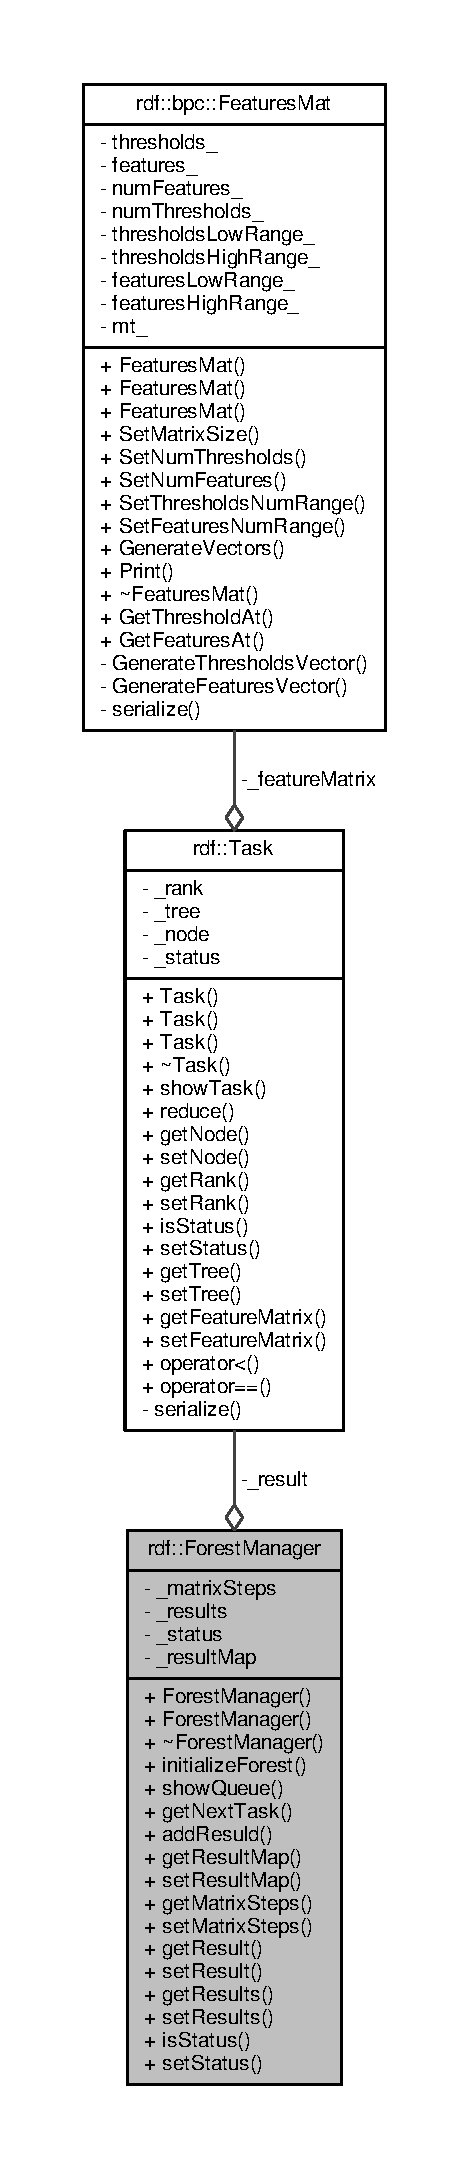
\includegraphics[height=550pt]{classrdf_1_1ForestManager__coll__graph}
\end{center}
\end{figure}
\subsection*{Public Member Functions}
\begin{DoxyCompactItemize}
\item 
\hyperlink{classrdf_1_1ForestManager_a91a1f9806518ed82227b382bc4427c56}{Forest\+Manager} ()
\item 
\hyperlink{classrdf_1_1ForestManager_a5ca6326452d58bd367459b00bf893eae}{Forest\+Manager} (const \hyperlink{classrdf_1_1ForestManager}{Forest\+Manager} \&orig)
\item 
virtual \hyperlink{classrdf_1_1ForestManager_a99e383aec1205f1f664047a9e6e22a10}{$\sim$\+Forest\+Manager} ()
\item 
void \hyperlink{classrdf_1_1ForestManager_abfc6d077d99b06b8d135d114f477ad5f}{initialize\+Forest} ()
\item 
void \hyperlink{classrdf_1_1ForestManager_af8975e5a2ea89cf3477241ebf7915ebe}{show\+Queue} ()
\item 
\hyperlink{classrdf_1_1Task}{Task} \& \hyperlink{classrdf_1_1ForestManager_a7531fb627d10ebcf471237449864317e}{get\+Next\+Task} ()
\item 
bool \hyperlink{classrdf_1_1ForestManager_a1399d029371b213523492ea8397199b6}{add\+Resuld} (\hyperlink{classrdf_1_1NodeResult}{rdf\+::\+Node\+Result} \&p\+Result)
\item 
std\+::map$<$ \hyperlink{classrdf_1_1Task}{Task}, \hyperlink{classrdf_1_1NodeResult}{rdf\+::\+Node\+Result} $>$ \hyperlink{classrdf_1_1ForestManager_aaacb6fcbb2b7a71f017fa49e4b0f813c}{get\+Result\+Map} () const 
\item 
void \hyperlink{classrdf_1_1ForestManager_ab88e04c863d4b6565670a65fe5b06435}{set\+Result\+Map} (std\+::map$<$ \hyperlink{classrdf_1_1Task}{Task}, \hyperlink{classrdf_1_1NodeResult}{rdf\+::\+Node\+Result} $>$ \hyperlink{classrdf_1_1ForestManager_ad764e01a338ea42ad8b2eaf360971875}{\+\_\+result\+Map})
\item 
vector$<$ \hyperlink{classrdf_1_1Task}{Task} $>$ \hyperlink{classrdf_1_1ForestManager_a6ff0f37f87dab897d449aa453e559926}{get\+Matrix\+Steps} () const 
\item 
void \hyperlink{classrdf_1_1ForestManager_a99315a804dfb3d3a70f0163eb9a245d8}{set\+Matrix\+Steps} (vector$<$ \hyperlink{classrdf_1_1Task}{rdf\+::\+Task} $>$ \hyperlink{classrdf_1_1ForestManager_a34fac652fc47cf8af5f7b292219d85ed}{\+\_\+matrix\+Steps})
\item 
\hyperlink{classrdf_1_1Task}{rdf\+::\+Task} \hyperlink{classrdf_1_1ForestManager_a6de8eeda582a53feee2127d1bf71b975}{get\+Result} () const 
\item 
void \hyperlink{classrdf_1_1ForestManager_af54eefeab5a70439d23ebf43fc549e6d}{set\+Result} (\hyperlink{classrdf_1_1Task}{rdf\+::\+Task} \hyperlink{classrdf_1_1ForestManager_ae2ba9a9f403d88f6343cf374d69f8a17}{\+\_\+result})
\item 
vector$<$ vector$<$ \hyperlink{classrdf_1_1NodeResult}{rdf\+::\+Node\+Result} $>$ $>$ \hyperlink{classrdf_1_1ForestManager_a009d3210babe33268dcf5e5698cfaeca}{get\+Results} () const 
\item 
void \hyperlink{classrdf_1_1ForestManager_a2e03f8ee1756620a2f528c28be13009b}{set\+Results} (vector$<$ vector$<$ \hyperlink{classrdf_1_1NodeResult}{rdf\+::\+Node\+Result} $>$ $>$ \hyperlink{classrdf_1_1ForestManager_a818d29de52bed7f09084c71d687ddd4f}{\+\_\+results})
\item 
bool \hyperlink{classrdf_1_1ForestManager_a90ec517ef47983b2d8998a8eafe46ecc}{is\+Status} () const 
\item 
void \hyperlink{classrdf_1_1ForestManager_af141b0f89158084ff1e777141dae69f2}{set\+Status} (bool \hyperlink{classrdf_1_1ForestManager_a8aa48a6543d83bf43be3b0bc8a8ab253}{\+\_\+status})
\end{DoxyCompactItemize}
\subsection*{Private Attributes}
\begin{DoxyCompactItemize}
\item 
vector$<$ \hyperlink{classrdf_1_1Task}{rdf\+::\+Task} $>$ \hyperlink{classrdf_1_1ForestManager_a34fac652fc47cf8af5f7b292219d85ed}{\+\_\+matrix\+Steps}
\item 
vector$<$ vector$<$ \hyperlink{classrdf_1_1NodeResult}{rdf\+::\+Node\+Result} $>$ $>$ \hyperlink{classrdf_1_1ForestManager_a818d29de52bed7f09084c71d687ddd4f}{\+\_\+results}
\item 
bool \hyperlink{classrdf_1_1ForestManager_a8aa48a6543d83bf43be3b0bc8a8ab253}{\+\_\+status}
\item 
\hyperlink{classrdf_1_1Task}{Task} \hyperlink{classrdf_1_1ForestManager_ae2ba9a9f403d88f6343cf374d69f8a17}{\+\_\+result}
\item 
std\+::map$<$ \hyperlink{classrdf_1_1Task}{Task}, \hyperlink{classrdf_1_1NodeResult}{rdf\+::\+Node\+Result} $>$ \hyperlink{classrdf_1_1ForestManager_ad764e01a338ea42ad8b2eaf360971875}{\+\_\+result\+Map}
\end{DoxyCompactItemize}


\subsection{Detailed Description}
Thisclass allow manage train nodes, trees. 

\subsection{Constructor \& Destructor Documentation}
\index{rdf\+::\+Forest\+Manager@{rdf\+::\+Forest\+Manager}!Forest\+Manager@{Forest\+Manager}}
\index{Forest\+Manager@{Forest\+Manager}!rdf\+::\+Forest\+Manager@{rdf\+::\+Forest\+Manager}}
\subsubsection[{\texorpdfstring{Forest\+Manager()}{ForestManager()}}]{\setlength{\rightskip}{0pt plus 5cm}rdf\+::\+Forest\+Manager\+::\+Forest\+Manager (
\begin{DoxyParamCaption}
{}
\end{DoxyParamCaption}
)}\hypertarget{classrdf_1_1ForestManager_a91a1f9806518ed82227b382bc4427c56}{}\label{classrdf_1_1ForestManager_a91a1f9806518ed82227b382bc4427c56}


References \+\_\+status.


\begin{DoxyCode}
16                                 \{
17     \hyperlink{classrdf_1_1ForestManager_a8aa48a6543d83bf43be3b0bc8a8ab253}{\_status}=\textcolor{keyword}{false};
18 \}
\end{DoxyCode}
\index{rdf\+::\+Forest\+Manager@{rdf\+::\+Forest\+Manager}!Forest\+Manager@{Forest\+Manager}}
\index{Forest\+Manager@{Forest\+Manager}!rdf\+::\+Forest\+Manager@{rdf\+::\+Forest\+Manager}}
\subsubsection[{\texorpdfstring{Forest\+Manager(const Forest\+Manager \&orig)}{ForestManager(const ForestManager &orig)}}]{\setlength{\rightskip}{0pt plus 5cm}rdf\+::\+Forest\+Manager\+::\+Forest\+Manager (
\begin{DoxyParamCaption}
\item[{const {\bf Forest\+Manager} \&}]{orig}
\end{DoxyParamCaption}
)}\hypertarget{classrdf_1_1ForestManager_a5ca6326452d58bd367459b00bf893eae}{}\label{classrdf_1_1ForestManager_a5ca6326452d58bd367459b00bf893eae}

\begin{DoxyCode}
20                                                          \{
21 \}
\end{DoxyCode}
\index{rdf\+::\+Forest\+Manager@{rdf\+::\+Forest\+Manager}!````~Forest\+Manager@{$\sim$\+Forest\+Manager}}
\index{````~Forest\+Manager@{$\sim$\+Forest\+Manager}!rdf\+::\+Forest\+Manager@{rdf\+::\+Forest\+Manager}}
\subsubsection[{\texorpdfstring{$\sim$\+Forest\+Manager()}{~ForestManager()}}]{\setlength{\rightskip}{0pt plus 5cm}rdf\+::\+Forest\+Manager\+::$\sim$\+Forest\+Manager (
\begin{DoxyParamCaption}
{}
\end{DoxyParamCaption}
)\hspace{0.3cm}{\ttfamily [virtual]}}\hypertarget{classrdf_1_1ForestManager_a99e383aec1205f1f664047a9e6e22a10}{}\label{classrdf_1_1ForestManager_a99e383aec1205f1f664047a9e6e22a10}

\begin{DoxyCode}
23                                  \{
24 \}
\end{DoxyCode}


\subsection{Member Function Documentation}
\index{rdf\+::\+Forest\+Manager@{rdf\+::\+Forest\+Manager}!add\+Resuld@{add\+Resuld}}
\index{add\+Resuld@{add\+Resuld}!rdf\+::\+Forest\+Manager@{rdf\+::\+Forest\+Manager}}
\subsubsection[{\texorpdfstring{add\+Resuld(rdf\+::\+Node\+Result \&p\+Result)}{addResuld(rdf::NodeResult &pResult)}}]{\setlength{\rightskip}{0pt plus 5cm}bool rdf\+::\+Forest\+Manager\+::add\+Resuld (
\begin{DoxyParamCaption}
\item[{{\bf rdf\+::\+Node\+Result} \&}]{p\+Result}
\end{DoxyParamCaption}
)}\hypertarget{classrdf_1_1ForestManager_a1399d029371b213523492ea8397199b6}{}\label{classrdf_1_1ForestManager_a1399d029371b213523492ea8397199b6}


References \+\_\+matrix\+Steps, \+\_\+result\+Map, rdf\+::\+Task\+::get\+Node(), rdf\+::\+Task\+::get\+Rank(), rdf\+::\+Node\+Result\+::get\+Result\+Size(), rdf\+::\+Node\+Result\+::get\+Task(), rdf\+::\+Task\+::get\+Tree(), rdf\+::\+Task\+::is\+Status(), rdf\+::\+Task\+::set\+Node(), rdf\+::\+Task\+::set\+Rank(), rdf\+::\+Task\+::set\+Status(), and rdf\+::\+Task\+::set\+Tree().



Referenced by rdf\+::\+Distribution\+Manager\+::waiting\+Results().


\begin{DoxyCode}
53                                                     \{
54     std::cout<<\textcolor{stringliteral}{"REDUCE: "} << pResult.\hyperlink{classrdf_1_1NodeResult_a47e07daae11352e753629f2fca98d526}{getResultSize}() << \textcolor{stringliteral}{"\(\backslash\)n"};
55 
56     \hyperlink{classrdf_1_1ForestManager_ad764e01a338ea42ad8b2eaf360971875}{\_resultMap}.find(pResult.\hyperlink{classrdf_1_1NodeResult_a564d581492a48333ed9796f6fd4b8c6a}{getTask}())->second.reduce(pResult);
57     \textcolor{comment}{//\_result.reduce(pResult);}
58     \textcolor{comment}{//\_result.showTask();}
59     
60     Task leftChild; 
61     Task rightChild;
62     
63     
64     leftChild.setRank(pResult.\hyperlink{classrdf_1_1NodeResult_a564d581492a48333ed9796f6fd4b8c6a}{getTask}().\hyperlink{classrdf_1_1Task_ab1bcd01480e2c381541b6346f15cf4b7}{getRank}());
65     leftChild.setTree(pResult.\hyperlink{classrdf_1_1NodeResult_a564d581492a48333ed9796f6fd4b8c6a}{getTask}().\hyperlink{classrdf_1_1Task_a942297717d39a25db9ed8636ef72dca1}{getTree}());
66     leftChild.setNode(2 * pResult.\hyperlink{classrdf_1_1NodeResult_a564d581492a48333ed9796f6fd4b8c6a}{getTask}().\hyperlink{classrdf_1_1Task_abed5b1d313483299a04f0ccb63901c54}{getNode}());
67     leftChild.setStatus(pResult.\hyperlink{classrdf_1_1NodeResult_a564d581492a48333ed9796f6fd4b8c6a}{getTask}().\hyperlink{classrdf_1_1Task_a2d78d32594b0c8f76a599cc3883211c7}{isStatus}());
68     
69     rightChild.setRank(pResult.\hyperlink{classrdf_1_1NodeResult_a564d581492a48333ed9796f6fd4b8c6a}{getTask}().\hyperlink{classrdf_1_1Task_ab1bcd01480e2c381541b6346f15cf4b7}{getRank}());
70     rightChild.setTree(pResult.\hyperlink{classrdf_1_1NodeResult_a564d581492a48333ed9796f6fd4b8c6a}{getTask}().\hyperlink{classrdf_1_1Task_a942297717d39a25db9ed8636ef72dca1}{getTree}());
71     rightChild.setNode(2 * pResult.\hyperlink{classrdf_1_1NodeResult_a564d581492a48333ed9796f6fd4b8c6a}{getTask}().\hyperlink{classrdf_1_1Task_abed5b1d313483299a04f0ccb63901c54}{getNode}()-1);
72     rightChild.setStatus(pResult.\hyperlink{classrdf_1_1NodeResult_a564d581492a48333ed9796f6fd4b8c6a}{getTask}().\hyperlink{classrdf_1_1Task_a2d78d32594b0c8f76a599cc3883211c7}{isStatus}());
73     
74     \hyperlink{classrdf_1_1ForestManager_a34fac652fc47cf8af5f7b292219d85ed}{\_matrixSteps}.push\_back(leftChild);
75     \hyperlink{classrdf_1_1ForestManager_a34fac652fc47cf8af5f7b292219d85ed}{\_matrixSteps}.push\_back(rightChild);
76     std::cout<< \textcolor{stringliteral}{"Adding child nodes, size: "}<<\hyperlink{classrdf_1_1ForestManager_a34fac652fc47cf8af5f7b292219d85ed}{\_matrixSteps}.size()<<\textcolor{stringliteral}{"\(\backslash\)n"};
77     NodeResult result;
78     
79     \hyperlink{classrdf_1_1ForestManager_ad764e01a338ea42ad8b2eaf360971875}{\_resultMap}.insert(std::make\_pair(leftChild,result));
80     \hyperlink{classrdf_1_1ForestManager_ad764e01a338ea42ad8b2eaf360971875}{\_resultMap}.insert(std::make\_pair(leftChild,result));
81     
82     \textcolor{comment}{//leftChild.showTask();}
83     \textcolor{comment}{//rightChild.showTask();}
84     
85     
86     
87 
88     \textcolor{keywordflow}{return} \textcolor{keyword}{true};
89 
90 \}
\end{DoxyCode}
\index{rdf\+::\+Forest\+Manager@{rdf\+::\+Forest\+Manager}!get\+Matrix\+Steps@{get\+Matrix\+Steps}}
\index{get\+Matrix\+Steps@{get\+Matrix\+Steps}!rdf\+::\+Forest\+Manager@{rdf\+::\+Forest\+Manager}}
\subsubsection[{\texorpdfstring{get\+Matrix\+Steps() const }{getMatrixSteps() const }}]{\setlength{\rightskip}{0pt plus 5cm}vector$<${\bf Task}$>$ rdf\+::\+Forest\+Manager\+::get\+Matrix\+Steps (
\begin{DoxyParamCaption}
{}
\end{DoxyParamCaption}
) const\hspace{0.3cm}{\ttfamily [inline]}}\hypertarget{classrdf_1_1ForestManager_a6ff0f37f87dab897d449aa453e559926}{}\label{classrdf_1_1ForestManager_a6ff0f37f87dab897d449aa453e559926}

\begin{DoxyCode}
60                                                 \{
61                 \textcolor{keywordflow}{return} \hyperlink{classrdf_1_1ForestManager_a34fac652fc47cf8af5f7b292219d85ed}{\_matrixSteps};
62             \}
\end{DoxyCode}
\index{rdf\+::\+Forest\+Manager@{rdf\+::\+Forest\+Manager}!get\+Next\+Task@{get\+Next\+Task}}
\index{get\+Next\+Task@{get\+Next\+Task}!rdf\+::\+Forest\+Manager@{rdf\+::\+Forest\+Manager}}
\subsubsection[{\texorpdfstring{get\+Next\+Task()}{getNextTask()}}]{\setlength{\rightskip}{0pt plus 5cm}{\bf rdf\+::\+Task} \& rdf\+::\+Forest\+Manager\+::get\+Next\+Task (
\begin{DoxyParamCaption}
{}
\end{DoxyParamCaption}
)}\hypertarget{classrdf_1_1ForestManager_a7531fb627d10ebcf471237449864317e}{}\label{classrdf_1_1ForestManager_a7531fb627d10ebcf471237449864317e}


References \+\_\+matrix\+Steps.


\begin{DoxyCode}
46                                         \{
47     std::cout << \textcolor{stringliteral}{"Queue Size: "} << \hyperlink{classrdf_1_1ForestManager_a34fac652fc47cf8af5f7b292219d85ed}{\_matrixSteps}.size()<< \textcolor{stringliteral}{"\(\backslash\)n"};
48     \hyperlink{classrdf_1_1Task}{rdf::Task} &test = \hyperlink{classrdf_1_1ForestManager_a34fac652fc47cf8af5f7b292219d85ed}{\_matrixSteps}[0];
49     \textcolor{comment}{//\_matrixSteps.erase(\_matrixSteps.begin());}
50     \textcolor{keywordflow}{return} test;
51 \}
\end{DoxyCode}
\index{rdf\+::\+Forest\+Manager@{rdf\+::\+Forest\+Manager}!get\+Result@{get\+Result}}
\index{get\+Result@{get\+Result}!rdf\+::\+Forest\+Manager@{rdf\+::\+Forest\+Manager}}
\subsubsection[{\texorpdfstring{get\+Result() const }{getResult() const }}]{\setlength{\rightskip}{0pt plus 5cm}{\bf rdf\+::\+Task} rdf\+::\+Forest\+Manager\+::get\+Result (
\begin{DoxyParamCaption}
{}
\end{DoxyParamCaption}
) const\hspace{0.3cm}{\ttfamily [inline]}}\hypertarget{classrdf_1_1ForestManager_a6de8eeda582a53feee2127d1bf71b975}{}\label{classrdf_1_1ForestManager_a6de8eeda582a53feee2127d1bf71b975}

\begin{DoxyCode}
69                                       \{
70                 \textcolor{keywordflow}{return} \hyperlink{classrdf_1_1ForestManager_ae2ba9a9f403d88f6343cf374d69f8a17}{\_result};
71             \}
\end{DoxyCode}
\index{rdf\+::\+Forest\+Manager@{rdf\+::\+Forest\+Manager}!get\+Result\+Map@{get\+Result\+Map}}
\index{get\+Result\+Map@{get\+Result\+Map}!rdf\+::\+Forest\+Manager@{rdf\+::\+Forest\+Manager}}
\subsubsection[{\texorpdfstring{get\+Result\+Map() const }{getResultMap() const }}]{\setlength{\rightskip}{0pt plus 5cm}std\+::map$<${\bf Task}, {\bf rdf\+::\+Node\+Result}$>$ rdf\+::\+Forest\+Manager\+::get\+Result\+Map (
\begin{DoxyParamCaption}
{}
\end{DoxyParamCaption}
) const\hspace{0.3cm}{\ttfamily [inline]}}\hypertarget{classrdf_1_1ForestManager_aaacb6fcbb2b7a71f017fa49e4b0f813c}{}\label{classrdf_1_1ForestManager_aaacb6fcbb2b7a71f017fa49e4b0f813c}

\begin{DoxyCode}
52                                                              \{
53                 \textcolor{keywordflow}{return} \hyperlink{classrdf_1_1ForestManager_ad764e01a338ea42ad8b2eaf360971875}{\_resultMap};
54             \}
\end{DoxyCode}
\index{rdf\+::\+Forest\+Manager@{rdf\+::\+Forest\+Manager}!get\+Results@{get\+Results}}
\index{get\+Results@{get\+Results}!rdf\+::\+Forest\+Manager@{rdf\+::\+Forest\+Manager}}
\subsubsection[{\texorpdfstring{get\+Results() const }{getResults() const }}]{\setlength{\rightskip}{0pt plus 5cm}vector$<$vector$<${\bf rdf\+::\+Node\+Result}$>$ $>$ rdf\+::\+Forest\+Manager\+::get\+Results (
\begin{DoxyParamCaption}
{}
\end{DoxyParamCaption}
) const\hspace{0.3cm}{\ttfamily [inline]}}\hypertarget{classrdf_1_1ForestManager_a009d3210babe33268dcf5e5698cfaeca}{}\label{classrdf_1_1ForestManager_a009d3210babe33268dcf5e5698cfaeca}

\begin{DoxyCode}
75                                                               \{
76                 \textcolor{keywordflow}{return} \hyperlink{classrdf_1_1ForestManager_a818d29de52bed7f09084c71d687ddd4f}{\_results};
77             \}
\end{DoxyCode}
\index{rdf\+::\+Forest\+Manager@{rdf\+::\+Forest\+Manager}!initialize\+Forest@{initialize\+Forest}}
\index{initialize\+Forest@{initialize\+Forest}!rdf\+::\+Forest\+Manager@{rdf\+::\+Forest\+Manager}}
\subsubsection[{\texorpdfstring{initialize\+Forest()}{initializeForest()}}]{\setlength{\rightskip}{0pt plus 5cm}void rdf\+::\+Forest\+Manager\+::initialize\+Forest (
\begin{DoxyParamCaption}
{}
\end{DoxyParamCaption}
)}\hypertarget{classrdf_1_1ForestManager_abfc6d077d99b06b8d135d114f477ad5f}{}\label{classrdf_1_1ForestManager_abfc6d077d99b06b8d135d114f477ad5f}


References \+\_\+matrix\+Steps, \+\_\+result\+Map, rdf\+::\+Task\+::set\+Node(), rdf\+::\+Task\+::set\+Rank(), rdf\+::\+Task\+::set\+Status(), rdf\+::\+Task\+::set\+Tree(), and T\+R\+E\+E\+\_\+\+A\+M\+O\+U\+NT.


\begin{DoxyCode}
26                                         \{
27     \textcolor{keywordflow}{for}(\textcolor{keywordtype}{int} i = 0; i < \hyperlink{Config_8h_a534cdc6cb39fa1f6fc95a92491cab5fb}{TREE\_AMOUNT}; i++)\{
28         \hyperlink{classrdf_1_1Task}{rdf::Task} newTask;
29         newTask.\hyperlink{classrdf_1_1Task_aa55d27b31ed812e31e21fa5676208f1b}{setRank}(0);
30         newTask.\hyperlink{classrdf_1_1Task_ad7948910883a02524a0975d47c1827a7}{setTree}(i);
31         newTask.\hyperlink{classrdf_1_1Task_aa7667e08b39f5b6cae63aa0abeb4c412}{setNode}(1);
32         newTask.\hyperlink{classrdf_1_1Task_af030aac32a3943f2cd0fb22c8e964071}{setStatus}(\textcolor{keyword}{false}); 
33         \hyperlink{classrdf_1_1ForestManager_a34fac652fc47cf8af5f7b292219d85ed}{\_matrixSteps}.push\_back(newTask);
34         \hyperlink{classrdf_1_1NodeResult}{rdf::NodeResult} \hyperlink{structQueueTask_1_1TaskStruct_a22eb8e22f500809266c4983897b9af7f}{node}; 
35         \hyperlink{classrdf_1_1ForestManager_ad764e01a338ea42ad8b2eaf360971875}{\_resultMap}.insert(std::make\_pair(newTask,node));
36     \} 
37 \}
\end{DoxyCode}
\index{rdf\+::\+Forest\+Manager@{rdf\+::\+Forest\+Manager}!is\+Status@{is\+Status}}
\index{is\+Status@{is\+Status}!rdf\+::\+Forest\+Manager@{rdf\+::\+Forest\+Manager}}
\subsubsection[{\texorpdfstring{is\+Status() const }{isStatus() const }}]{\setlength{\rightskip}{0pt plus 5cm}bool rdf\+::\+Forest\+Manager\+::is\+Status (
\begin{DoxyParamCaption}
{}
\end{DoxyParamCaption}
) const\hspace{0.3cm}{\ttfamily [inline]}}\hypertarget{classrdf_1_1ForestManager_a90ec517ef47983b2d8998a8eafe46ecc}{}\label{classrdf_1_1ForestManager_a90ec517ef47983b2d8998a8eafe46ecc}

\begin{DoxyCode}
83                                   \{
84                 \textcolor{keywordflow}{return} \hyperlink{classrdf_1_1ForestManager_a8aa48a6543d83bf43be3b0bc8a8ab253}{\_status};
85             \}
\end{DoxyCode}
\index{rdf\+::\+Forest\+Manager@{rdf\+::\+Forest\+Manager}!set\+Matrix\+Steps@{set\+Matrix\+Steps}}
\index{set\+Matrix\+Steps@{set\+Matrix\+Steps}!rdf\+::\+Forest\+Manager@{rdf\+::\+Forest\+Manager}}
\subsubsection[{\texorpdfstring{set\+Matrix\+Steps(vector$<$ rdf\+::\+Task $>$ \+\_\+matrix\+Steps)}{setMatrixSteps(vector< rdf::Task > _matrixSteps)}}]{\setlength{\rightskip}{0pt plus 5cm}void rdf\+::\+Forest\+Manager\+::set\+Matrix\+Steps (
\begin{DoxyParamCaption}
\item[{vector$<$ {\bf rdf\+::\+Task} $>$}]{\+\_\+matrix\+Steps}
\end{DoxyParamCaption}
)\hspace{0.3cm}{\ttfamily [inline]}}\hypertarget{classrdf_1_1ForestManager_a99315a804dfb3d3a70f0163eb9a245d8}{}\label{classrdf_1_1ForestManager_a99315a804dfb3d3a70f0163eb9a245d8}

\begin{DoxyCode}
64                                                               \{
65                 this->\hyperlink{classrdf_1_1ForestManager_a34fac652fc47cf8af5f7b292219d85ed}{\_matrixSteps} = \hyperlink{classrdf_1_1ForestManager_a34fac652fc47cf8af5f7b292219d85ed}{\_matrixSteps};
66             \}
\end{DoxyCode}
\index{rdf\+::\+Forest\+Manager@{rdf\+::\+Forest\+Manager}!set\+Result@{set\+Result}}
\index{set\+Result@{set\+Result}!rdf\+::\+Forest\+Manager@{rdf\+::\+Forest\+Manager}}
\subsubsection[{\texorpdfstring{set\+Result(rdf\+::\+Task \+\_\+result)}{setResult(rdf::Task _result)}}]{\setlength{\rightskip}{0pt plus 5cm}void rdf\+::\+Forest\+Manager\+::set\+Result (
\begin{DoxyParamCaption}
\item[{{\bf rdf\+::\+Task}}]{\+\_\+result}
\end{DoxyParamCaption}
)\hspace{0.3cm}{\ttfamily [inline]}}\hypertarget{classrdf_1_1ForestManager_af54eefeab5a70439d23ebf43fc549e6d}{}\label{classrdf_1_1ForestManager_af54eefeab5a70439d23ebf43fc549e6d}

\begin{DoxyCode}
72                                             \{
73                 this->\_result = \hyperlink{classrdf_1_1ForestManager_ae2ba9a9f403d88f6343cf374d69f8a17}{\_result};
74             \}
\end{DoxyCode}
\index{rdf\+::\+Forest\+Manager@{rdf\+::\+Forest\+Manager}!set\+Result\+Map@{set\+Result\+Map}}
\index{set\+Result\+Map@{set\+Result\+Map}!rdf\+::\+Forest\+Manager@{rdf\+::\+Forest\+Manager}}
\subsubsection[{\texorpdfstring{set\+Result\+Map(std\+::map$<$ Task, rdf\+::\+Node\+Result $>$ \+\_\+result\+Map)}{setResultMap(std::map< Task, rdf::NodeResult > _resultMap)}}]{\setlength{\rightskip}{0pt plus 5cm}void rdf\+::\+Forest\+Manager\+::set\+Result\+Map (
\begin{DoxyParamCaption}
\item[{std\+::map$<$ {\bf Task}, {\bf rdf\+::\+Node\+Result} $>$}]{\+\_\+result\+Map}
\end{DoxyParamCaption}
)\hspace{0.3cm}{\ttfamily [inline]}}\hypertarget{classrdf_1_1ForestManager_ab88e04c863d4b6565670a65fe5b06435}{}\label{classrdf_1_1ForestManager_ab88e04c863d4b6565670a65fe5b06435}

\begin{DoxyCode}
56                                                                       \{
57                 this->\hyperlink{classrdf_1_1ForestManager_ad764e01a338ea42ad8b2eaf360971875}{\_resultMap} = \hyperlink{classrdf_1_1ForestManager_ad764e01a338ea42ad8b2eaf360971875}{\_resultMap};
58             \}
\end{DoxyCode}
\index{rdf\+::\+Forest\+Manager@{rdf\+::\+Forest\+Manager}!set\+Results@{set\+Results}}
\index{set\+Results@{set\+Results}!rdf\+::\+Forest\+Manager@{rdf\+::\+Forest\+Manager}}
\subsubsection[{\texorpdfstring{set\+Results(vector$<$ vector$<$ rdf\+::\+Node\+Result $>$ $>$ \+\_\+results)}{setResults(vector< vector< rdf::NodeResult > > _results)}}]{\setlength{\rightskip}{0pt plus 5cm}void rdf\+::\+Forest\+Manager\+::set\+Results (
\begin{DoxyParamCaption}
\item[{vector$<$ vector$<$ {\bf rdf\+::\+Node\+Result} $>$ $>$}]{\+\_\+results}
\end{DoxyParamCaption}
)\hspace{0.3cm}{\ttfamily [inline]}}\hypertarget{classrdf_1_1ForestManager_a2e03f8ee1756620a2f528c28be13009b}{}\label{classrdf_1_1ForestManager_a2e03f8ee1756620a2f528c28be13009b}

\begin{DoxyCode}
79                                                                      \{
80                 this->\hyperlink{classrdf_1_1ForestManager_a818d29de52bed7f09084c71d687ddd4f}{\_results} = \hyperlink{classrdf_1_1ForestManager_a818d29de52bed7f09084c71d687ddd4f}{\_results};
81             \}
\end{DoxyCode}
\index{rdf\+::\+Forest\+Manager@{rdf\+::\+Forest\+Manager}!set\+Status@{set\+Status}}
\index{set\+Status@{set\+Status}!rdf\+::\+Forest\+Manager@{rdf\+::\+Forest\+Manager}}
\subsubsection[{\texorpdfstring{set\+Status(bool \+\_\+status)}{setStatus(bool _status)}}]{\setlength{\rightskip}{0pt plus 5cm}void rdf\+::\+Forest\+Manager\+::set\+Status (
\begin{DoxyParamCaption}
\item[{bool}]{\+\_\+status}
\end{DoxyParamCaption}
)\hspace{0.3cm}{\ttfamily [inline]}}\hypertarget{classrdf_1_1ForestManager_af141b0f89158084ff1e777141dae69f2}{}\label{classrdf_1_1ForestManager_af141b0f89158084ff1e777141dae69f2}

\begin{DoxyCode}
87                                          \{
88                 this->\hyperlink{classrdf_1_1ForestManager_a8aa48a6543d83bf43be3b0bc8a8ab253}{\_status} = \hyperlink{classrdf_1_1ForestManager_a8aa48a6543d83bf43be3b0bc8a8ab253}{\_status};
89             \}
\end{DoxyCode}
\index{rdf\+::\+Forest\+Manager@{rdf\+::\+Forest\+Manager}!show\+Queue@{show\+Queue}}
\index{show\+Queue@{show\+Queue}!rdf\+::\+Forest\+Manager@{rdf\+::\+Forest\+Manager}}
\subsubsection[{\texorpdfstring{show\+Queue()}{showQueue()}}]{\setlength{\rightskip}{0pt plus 5cm}void rdf\+::\+Forest\+Manager\+::show\+Queue (
\begin{DoxyParamCaption}
{}
\end{DoxyParamCaption}
)}\hypertarget{classrdf_1_1ForestManager_af8975e5a2ea89cf3477241ebf7915ebe}{}\label{classrdf_1_1ForestManager_af8975e5a2ea89cf3477241ebf7915ebe}


References \+\_\+matrix\+Steps, and rdf\+::\+Task\+::show\+Task().



Referenced by rdf\+::\+Distribution\+Manager\+::waiting\+Results().


\begin{DoxyCode}
39                                  \{
40     \textcolor{keywordflow}{for}(\textcolor{keywordtype}{int} i=0; i<\hyperlink{classrdf_1_1ForestManager_a34fac652fc47cf8af5f7b292219d85ed}{\_matrixSteps}.size(); i++)\{
41         \hyperlink{classrdf_1_1Task}{rdf::Task} temp = \hyperlink{classrdf_1_1ForestManager_a34fac652fc47cf8af5f7b292219d85ed}{\_matrixSteps}[i];
42         temp.\hyperlink{classrdf_1_1Task_aed5f96455f9684078a5fa8fce849d197}{showTask}();
43     \}
44 \}
\end{DoxyCode}


\subsection{Member Data Documentation}
\index{rdf\+::\+Forest\+Manager@{rdf\+::\+Forest\+Manager}!\+\_\+matrix\+Steps@{\+\_\+matrix\+Steps}}
\index{\+\_\+matrix\+Steps@{\+\_\+matrix\+Steps}!rdf\+::\+Forest\+Manager@{rdf\+::\+Forest\+Manager}}
\subsubsection[{\texorpdfstring{\+\_\+matrix\+Steps}{_matrixSteps}}]{\setlength{\rightskip}{0pt plus 5cm}vector$<${\bf rdf\+::\+Task}$>$ rdf\+::\+Forest\+Manager\+::\+\_\+matrix\+Steps\hspace{0.3cm}{\ttfamily [private]}}\hypertarget{classrdf_1_1ForestManager_a34fac652fc47cf8af5f7b292219d85ed}{}\label{classrdf_1_1ForestManager_a34fac652fc47cf8af5f7b292219d85ed}


Referenced by add\+Resuld(), get\+Next\+Task(), initialize\+Forest(), and show\+Queue().

\index{rdf\+::\+Forest\+Manager@{rdf\+::\+Forest\+Manager}!\+\_\+result@{\+\_\+result}}
\index{\+\_\+result@{\+\_\+result}!rdf\+::\+Forest\+Manager@{rdf\+::\+Forest\+Manager}}
\subsubsection[{\texorpdfstring{\+\_\+result}{_result}}]{\setlength{\rightskip}{0pt plus 5cm}{\bf Task} rdf\+::\+Forest\+Manager\+::\+\_\+result\hspace{0.3cm}{\ttfamily [private]}}\hypertarget{classrdf_1_1ForestManager_ae2ba9a9f403d88f6343cf374d69f8a17}{}\label{classrdf_1_1ForestManager_ae2ba9a9f403d88f6343cf374d69f8a17}
\index{rdf\+::\+Forest\+Manager@{rdf\+::\+Forest\+Manager}!\+\_\+result\+Map@{\+\_\+result\+Map}}
\index{\+\_\+result\+Map@{\+\_\+result\+Map}!rdf\+::\+Forest\+Manager@{rdf\+::\+Forest\+Manager}}
\subsubsection[{\texorpdfstring{\+\_\+result\+Map}{_resultMap}}]{\setlength{\rightskip}{0pt plus 5cm}std\+::map$<${\bf Task},{\bf rdf\+::\+Node\+Result}$>$ rdf\+::\+Forest\+Manager\+::\+\_\+result\+Map\hspace{0.3cm}{\ttfamily [private]}}\hypertarget{classrdf_1_1ForestManager_ad764e01a338ea42ad8b2eaf360971875}{}\label{classrdf_1_1ForestManager_ad764e01a338ea42ad8b2eaf360971875}


Referenced by add\+Resuld(), and initialize\+Forest().

\index{rdf\+::\+Forest\+Manager@{rdf\+::\+Forest\+Manager}!\+\_\+results@{\+\_\+results}}
\index{\+\_\+results@{\+\_\+results}!rdf\+::\+Forest\+Manager@{rdf\+::\+Forest\+Manager}}
\subsubsection[{\texorpdfstring{\+\_\+results}{_results}}]{\setlength{\rightskip}{0pt plus 5cm}vector$<$vector$<${\bf rdf\+::\+Node\+Result}$>$ $>$ rdf\+::\+Forest\+Manager\+::\+\_\+results\hspace{0.3cm}{\ttfamily [private]}}\hypertarget{classrdf_1_1ForestManager_a818d29de52bed7f09084c71d687ddd4f}{}\label{classrdf_1_1ForestManager_a818d29de52bed7f09084c71d687ddd4f}
\index{rdf\+::\+Forest\+Manager@{rdf\+::\+Forest\+Manager}!\+\_\+status@{\+\_\+status}}
\index{\+\_\+status@{\+\_\+status}!rdf\+::\+Forest\+Manager@{rdf\+::\+Forest\+Manager}}
\subsubsection[{\texorpdfstring{\+\_\+status}{_status}}]{\setlength{\rightskip}{0pt plus 5cm}bool rdf\+::\+Forest\+Manager\+::\+\_\+status\hspace{0.3cm}{\ttfamily [private]}}\hypertarget{classrdf_1_1ForestManager_a8aa48a6543d83bf43be3b0bc8a8ab253}{}\label{classrdf_1_1ForestManager_a8aa48a6543d83bf43be3b0bc8a8ab253}


Referenced by Forest\+Manager().



The documentation for this class was generated from the following files\+:\begin{DoxyCompactItemize}
\item 
\hyperlink{ForestManager_8h}{Forest\+Manager.\+h}\item 
\hyperlink{ForestManager_8cpp}{Forest\+Manager.\+cpp}\end{DoxyCompactItemize}

\hypertarget{classImage}{}\section{Image Class Reference}
\label{classImage}\index{Image@{Image}}


{\ttfamily \#include $<$Image.\+h$>$}



Collaboration diagram for Image\+:
\nopagebreak
\begin{figure}[H]
\begin{center}
\leavevmode
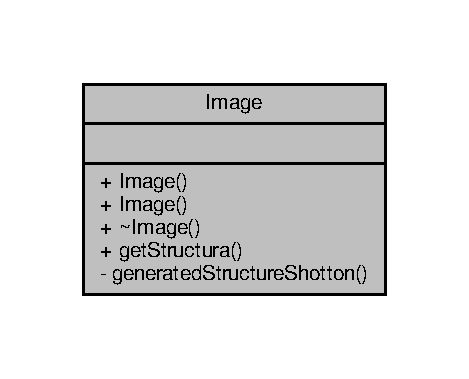
\includegraphics[width=225pt]{classImage__coll__graph}
\end{center}
\end{figure}
\subsection*{Public Member Functions}
\begin{DoxyCompactItemize}
\item 
\hyperlink{classImage_a58edd1c45b4faeb5f789b0d036d02313}{Image} ()
\item 
\hyperlink{classImage_abda271aa11b907dda8c8c8176684227d}{Image} (const \hyperlink{classImage}{Image} \&orig)
\item 
virtual \hyperlink{classImage_a0294f63700543e11c0f0da85601c7ae5}{$\sim$\+Image} ()
\item 
void \hyperlink{classImage_ad5ed787922c9c8aad26e1e349bdc4018}{get\+Structura} (std\+::vector$<$ \hyperlink{structEstructura_1_1Node}{Estructura\+::\+Node} $>$ \&structure, \hyperlink{structEstructura_1_1DataMaster}{Estructura\+::\+Data\+Master} data\+Master)
\end{DoxyCompactItemize}
\subsection*{Private Member Functions}
\begin{DoxyCompactItemize}
\item 
void \hyperlink{classImage_acc132bd92aec2c6186937566b593aafc}{generated\+Structure\+Shotton} (std\+::vector$<$ \hyperlink{structEstructura_1_1Node}{Estructura\+::\+Node} $>$ \&structure, std\+::string type\+\_\+\+Algorithm, int Num\+Points, int height, int width, int Num\+Tree, std\+::string path\+Depth, std\+::string pathlabel, int start\+Read, int end\+Read, int tree, int node)
\end{DoxyCompactItemize}


\subsection{Constructor \& Destructor Documentation}
\index{Image@{Image}!Image@{Image}}
\index{Image@{Image}!Image@{Image}}
\subsubsection[{\texorpdfstring{Image()}{Image()}}]{\setlength{\rightskip}{0pt plus 5cm}Image\+::\+Image (
\begin{DoxyParamCaption}
{}
\end{DoxyParamCaption}
)}\hypertarget{classImage_a58edd1c45b4faeb5f789b0d036d02313}{}\label{classImage_a58edd1c45b4faeb5f789b0d036d02313}

\begin{DoxyCode}
19              \{
20 \}
\end{DoxyCode}
\index{Image@{Image}!Image@{Image}}
\index{Image@{Image}!Image@{Image}}
\subsubsection[{\texorpdfstring{Image(const Image \&orig)}{Image(const Image &orig)}}]{\setlength{\rightskip}{0pt plus 5cm}Image\+::\+Image (
\begin{DoxyParamCaption}
\item[{const {\bf Image} \&}]{orig}
\end{DoxyParamCaption}
)}\hypertarget{classImage_abda271aa11b907dda8c8c8176684227d}{}\label{classImage_abda271aa11b907dda8c8c8176684227d}

\begin{DoxyCode}
22                               \{
23 \}
\end{DoxyCode}
\index{Image@{Image}!````~Image@{$\sim$\+Image}}
\index{````~Image@{$\sim$\+Image}!Image@{Image}}
\subsubsection[{\texorpdfstring{$\sim$\+Image()}{~Image()}}]{\setlength{\rightskip}{0pt plus 5cm}Image\+::$\sim$\+Image (
\begin{DoxyParamCaption}
{}
\end{DoxyParamCaption}
)\hspace{0.3cm}{\ttfamily [virtual]}}\hypertarget{classImage_a0294f63700543e11c0f0da85601c7ae5}{}\label{classImage_a0294f63700543e11c0f0da85601c7ae5}

\begin{DoxyCode}
25               \{
26 \}
\end{DoxyCode}


\subsection{Member Function Documentation}
\index{Image@{Image}!generated\+Structure\+Shotton@{generated\+Structure\+Shotton}}
\index{generated\+Structure\+Shotton@{generated\+Structure\+Shotton}!Image@{Image}}
\subsubsection[{\texorpdfstring{generated\+Structure\+Shotton(std\+::vector$<$ Estructura\+::\+Node $>$ \&structure, std\+::string type\+\_\+\+Algorithm, int Num\+Points, int height, int width, int Num\+Tree, std\+::string path\+Depth, std\+::string pathlabel, int start\+Read, int end\+Read, int tree, int node)}{generatedStructureShotton(std::vector< Estructura::Node > &structure, std::string type_Algorithm, int NumPoints, int height, int width, int NumTree, std::string pathDepth, std::string pathlabel, int startRead, int endRead, int tree, int node)}}]{\setlength{\rightskip}{0pt plus 5cm}void Image\+::generated\+Structure\+Shotton (
\begin{DoxyParamCaption}
\item[{std\+::vector$<$ {\bf Estructura\+::\+Node} $>$ \&}]{structure, }
\item[{std\+::string}]{type\+\_\+\+Algorithm, }
\item[{int}]{Num\+Points, }
\item[{int}]{height, }
\item[{int}]{width, }
\item[{int}]{Num\+Tree, }
\item[{std\+::string}]{path\+Depth, }
\item[{std\+::string}]{pathlabel, }
\item[{int}]{start\+Read, }
\item[{int}]{end\+Read, }
\item[{int}]{tree, }
\item[{int}]{node}
\end{DoxyParamCaption}
)\hspace{0.3cm}{\ttfamily [private]}}\hypertarget{classImage_acc132bd92aec2c6186937566b593aafc}{}\label{classImage_acc132bd92aec2c6186937566b593aafc}


References Points\+Select\+::generated\+Points(), Estructura\+::\+Node\+::image\+Depth, Estructura\+::\+Node\+::image\+Label, Estructura\+::\+Node\+::node, Estructura\+::\+Node\+::points, Collection\+::read\+Image(), Image\+Getter\+::read\+Path(), Collection\+::set\+Image(), and Estructura\+::\+Node\+::tree.



Referenced by get\+Structura().


\begin{DoxyCode}
46                                                         \{
47 
48     \hyperlink{classImageGetter}{ImageGetter} imageGetter;
49     \hyperlink{classLabelImage}{LabelImage} lblImage;
50     \hyperlink{classDepthImage}{DepthImage} depthImage;
51     \hyperlink{classCollection}{Collection} collection;
52     cv::Mat imageDepth, imageLabel;
53 
54     \textcolor{comment}{//lee las direciones del path}
55     std::vector<std::string> directionesDepth;
56     std::vector<std::string> directionesLabel;
57     \textcolor{keywordtype}{int} NumLines = 0;
58 
59     imageGetter.\hyperlink{classImageGetter_a92cd05c7e86df5bf83ee9f428a805fb3}{readPath}(directionesDepth, NumLines, pathDepth, startRead, endRead);
60     imageGetter.\hyperlink{classImageGetter_a92cd05c7e86df5bf83ee9f428a805fb3}{readPath}(directionesLabel, NumLines, pathlabel, startRead, endRead);
61 
62 
63 
64     \textcolor{comment}{// de aqui para arriba esta bien}
65 
66     \textcolor{keywordflow}{for} (\textcolor{keywordtype}{int} k = 0; k < directionesDepth.size(); k++) \{
67 
68         \hyperlink{structEstructura_1_1Node}{Estructura::Node} dataAll;
69         std::vector<Estructura::Pixel> puntos;
70         
71         \hyperlink{classEstructura}{Estructura} es;
72 
73         \hyperlink{classPointsSelect}{PointsSelect} pointSelect;
74         
75         
76         \textcolor{comment}{//leer la imagen de profundidad}
77         collection.\hyperlink{classCollection_a57290652c3cf6fc744c5614e0bf49d15}{setImage}(&depthImage);
78         collection.\hyperlink{classCollection_a251f7033e22c16a7b12dde94d9a7021e}{readImage}(height, width, directionesDepth[k], imageDepth);
79 
80         \textcolor{comment}{//leer la image de etiquetas}
81         collection.\hyperlink{classCollection_a57290652c3cf6fc744c5614e0bf49d15}{setImage}(&lblImage);
82         collection.\hyperlink{classCollection_a251f7033e22c16a7b12dde94d9a7021e}{readImage}(height, width, directionesLabel[k], imageLabel);
83 
84         \textcolor{comment}{//std::cout << imageLabel << "\(\backslash\)n";}
85         \textcolor{comment}{//para visualizar las imagenes que se estan cargando}
86         \textcolor{comment}{//es.seeImageDepth(height,width,imageDepth);}
87         \textcolor{comment}{//es.seeImageLabel(imageLabel);}
88 
89 
90 
91 
92         pointSelect.\hyperlink{classPointsSelect_a1c487676ff7dc9a8cfd7dbae206a04ae}{generatedPoints}(type\_Algorithm, puntos, NumPoints, height, width, 
      NumTree);
93 
94         \textcolor{comment}{//llena los campos y carga al vector}
95         dataAll.\hyperlink{structEstructura_1_1Node_a117720b249be79aaf71bc0a42d2c9b6b}{imageDepth} = imageDepth;
96         dataAll.\hyperlink{structEstructura_1_1Node_a7905c0696cb214e84ac855e7a6b6366c}{imageLabel} = imageLabel;
97         dataAll.\hyperlink{structEstructura_1_1Node_a0ad44a6cbbffdcd39f26733cc0e6f196}{points} = puntos;
98         dataAll.\hyperlink{structEstructura_1_1Node_a2e360ae2439d4d82dd38d9b30358feac}{node} = node;
99         dataAll.\hyperlink{structEstructura_1_1Node_abb400b36a5e8179766c35bc73c22e816}{tree} = tree;
100         structure.push\_back(dataAll);
101         
102     \}
103 
104 
105 \}\end{DoxyCode}
\index{Image@{Image}!get\+Structura@{get\+Structura}}
\index{get\+Structura@{get\+Structura}!Image@{Image}}
\subsubsection[{\texorpdfstring{get\+Structura(std\+::vector$<$ Estructura\+::\+Node $>$ \&structure, Estructura\+::\+Data\+Master data\+Master)}{getStructura(std::vector< Estructura::Node > &structure, Estructura::DataMaster dataMaster)}}]{\setlength{\rightskip}{0pt plus 5cm}void Image\+::get\+Structura (
\begin{DoxyParamCaption}
\item[{std\+::vector$<$ {\bf Estructura\+::\+Node} $>$ \&}]{structure, }
\item[{{\bf Estructura\+::\+Data\+Master}}]{data\+Master}
\end{DoxyParamCaption}
)}\hypertarget{classImage_ad5ed787922c9c8aad26e1e349bdc4018}{}\label{classImage_ad5ed787922c9c8aad26e1e349bdc4018}


References Estructura\+::\+Data\+Master\+::end\+Read, generated\+Structure\+Shotton(), Estructura\+::\+Data\+Master\+::height, Estructura\+::\+Data\+Master\+::node, Estructura\+::\+Data\+Master\+::\+Num\+Points, Estructura\+::\+Data\+Master\+::\+Num\+Tree, Estructura\+::\+Data\+Master\+::start\+Read, Estructura\+::\+Data\+Master\+::tree, Estructura\+::\+Data\+Master\+::type\+\_\+\+Algorithm, and Estructura\+::\+Data\+Master\+::width.



Referenced by Image\+Manager\+::load\+Images().


\begin{DoxyCode}
28                                                                                               \{
29     std::string PathDepthImage = \textcolor{stringliteral}{"/home/RDF/code/DistributedTrees/Database/pathDepth.txt"};
30     std::string PathLabelImage = \textcolor{stringliteral}{"/home/RDF/code/DistributedTrees/Database/pathLabel.txt"};
31 
32 
33     std::vector<Estructura::Node> structureTemp;
34     \textcolor{keywordflow}{if} (dataMaster.\hyperlink{structEstructura_1_1DataMaster_accae7ba56def5fd845b33cb8cfb384fe}{type\_Algorithm}.compare(0, 7, \textcolor{stringliteral}{"shotton"}) == 0) \{
35         \hyperlink{classImage_acc132bd92aec2c6186937566b593aafc}{generatedStructureShotton}(structureTemp, dataMaster.
      \hyperlink{structEstructura_1_1DataMaster_accae7ba56def5fd845b33cb8cfb384fe}{type\_Algorithm}, dataMaster.\hyperlink{structEstructura_1_1DataMaster_ad62760f62256a3fbd88481f720b81851}{NumPoints}, dataMaster.\hyperlink{structEstructura_1_1DataMaster_a33df1604c867e22af955f29c453d6651}{height}, dataMaster.
      \hyperlink{structEstructura_1_1DataMaster_a52e88b0d0d52d7e61880e3689ef2e638}{width},
36                 dataMaster.\hyperlink{structEstructura_1_1DataMaster_a950938f474870649fe7eceae940366fd}{NumTree}, PathDepthImage, PathLabelImage, dataMaster.
      \hyperlink{structEstructura_1_1DataMaster_ada49eb1401a3715858043ebd2b61c10c}{startRead}, dataMaster.\hyperlink{structEstructura_1_1DataMaster_a787807eccc80c8e639d2409477f37f3a}{endRead}, dataMaster.\hyperlink{structEstructura_1_1DataMaster_a766b1b437e0f242d3626a3759bef8b43}{tree}, dataMaster.
      \hyperlink{structEstructura_1_1DataMaster_a5b7bf8e1c983ad0a64dd596d1bb4e31a}{node});
37     \}
38 
39 
40     structure = structureTemp;
41 \}
\end{DoxyCode}


The documentation for this class was generated from the following files\+:\begin{DoxyCompactItemize}
\item 
\hyperlink{Image_8h}{Image.\+h}\item 
\hyperlink{Image_8cpp}{Image.\+cpp}\end{DoxyCompactItemize}

\hypertarget{classrdf_1_1ImageDispatcher}{}\section{rdf\+:\+:Image\+Dispatcher Class Reference}
\label{classrdf_1_1ImageDispatcher}\index{rdf\+::\+Image\+Dispatcher@{rdf\+::\+Image\+Dispatcher}}


{\ttfamily \#include $<$Image\+Dispatcher.\+h$>$}



Collaboration diagram for rdf\+:\+:Image\+Dispatcher\+:
\nopagebreak
\begin{figure}[H]
\begin{center}
\leavevmode
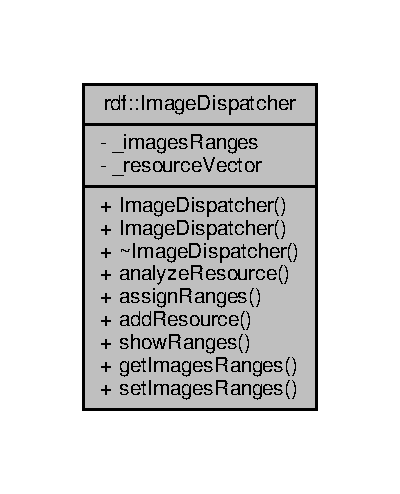
\includegraphics[width=192pt]{classrdf_1_1ImageDispatcher__coll__graph}
\end{center}
\end{figure}
\subsection*{Public Member Functions}
\begin{DoxyCompactItemize}
\item 
\hyperlink{classrdf_1_1ImageDispatcher_a32ca43231de0932370b3b5a98f76f5b5}{Image\+Dispatcher} ()
\item 
\hyperlink{classrdf_1_1ImageDispatcher_a75d599869487a60fcaf0269f77f2c049}{Image\+Dispatcher} (const \hyperlink{classrdf_1_1ImageDispatcher}{Image\+Dispatcher} \&orig)
\item 
virtual \hyperlink{classrdf_1_1ImageDispatcher_ab7a10dc991075876919a0d657251c808}{$\sim$\+Image\+Dispatcher} ()
\item 
int \hyperlink{classrdf_1_1ImageDispatcher_a0fe89ed7467fd34e1e24984b87d6d3bc}{analyze\+Resource} (\hyperlink{classrdf_1_1Resource}{rdf\+::\+Resource} \&p\+Resource)
\item 
void \hyperlink{classrdf_1_1ImageDispatcher_a10e89cb9630fe93877a23f485d2a1213}{assign\+Ranges} (int p\+Intervals, bool p\+Flag)
\item 
void \hyperlink{classrdf_1_1ImageDispatcher_a900b639d7be2ac5e4e48b5a7aa879182}{add\+Resource} (\hyperlink{classrdf_1_1Resource}{rdf\+::\+Resource} \&p\+Resource)
\item 
void \hyperlink{classrdf_1_1ImageDispatcher_ac78db12cfd581737ad8077e0af974c2b}{show\+Ranges} ()
\item 
std\+::vector$<$ std\+::pair$<$ int, int $>$ $>$ \hyperlink{classrdf_1_1ImageDispatcher_a1044b93dabc737e15045fc5c62970e7b}{get\+Images\+Ranges} () const 
\item 
void \hyperlink{classrdf_1_1ImageDispatcher_a989c61bb935fa54a0838bd2d49a51133}{set\+Images\+Ranges} (std\+::vector$<$ std\+::pair$<$ int, int $>$ $>$ \hyperlink{classrdf_1_1ImageDispatcher_a090ae3aa3b2e08ebc0432314ef519ae6}{\+\_\+images\+Ranges})
\end{DoxyCompactItemize}
\subsection*{Private Attributes}
\begin{DoxyCompactItemize}
\item 
std\+::vector$<$ std\+::pair$<$ int, int $>$ $>$ \hyperlink{classrdf_1_1ImageDispatcher_a090ae3aa3b2e08ebc0432314ef519ae6}{\+\_\+images\+Ranges}
\item 
std\+::vector$<$ \hyperlink{classrdf_1_1Resource}{rdf\+::\+Resource} $>$ \hyperlink{classrdf_1_1ImageDispatcher_aee49acec382a35bd2043e14f56dce8b1}{\+\_\+resource\+Vector}
\end{DoxyCompactItemize}


\subsection{Detailed Description}
\textquotesingle{} This class identify resources from all different nodes and say how many images this node can load to the memory 

\subsection{Constructor \& Destructor Documentation}
\index{rdf\+::\+Image\+Dispatcher@{rdf\+::\+Image\+Dispatcher}!Image\+Dispatcher@{Image\+Dispatcher}}
\index{Image\+Dispatcher@{Image\+Dispatcher}!rdf\+::\+Image\+Dispatcher@{rdf\+::\+Image\+Dispatcher}}
\subsubsection[{\texorpdfstring{Image\+Dispatcher()}{ImageDispatcher()}}]{\setlength{\rightskip}{0pt plus 5cm}rdf\+::\+Image\+Dispatcher\+::\+Image\+Dispatcher (
\begin{DoxyParamCaption}
{}
\end{DoxyParamCaption}
)}\hypertarget{classrdf_1_1ImageDispatcher_a32ca43231de0932370b3b5a98f76f5b5}{}\label{classrdf_1_1ImageDispatcher_a32ca43231de0932370b3b5a98f76f5b5}

\begin{DoxyCode}
19                                     \{
20 \}
\end{DoxyCode}
\index{rdf\+::\+Image\+Dispatcher@{rdf\+::\+Image\+Dispatcher}!Image\+Dispatcher@{Image\+Dispatcher}}
\index{Image\+Dispatcher@{Image\+Dispatcher}!rdf\+::\+Image\+Dispatcher@{rdf\+::\+Image\+Dispatcher}}
\subsubsection[{\texorpdfstring{Image\+Dispatcher(const Image\+Dispatcher \&orig)}{ImageDispatcher(const ImageDispatcher &orig)}}]{\setlength{\rightskip}{0pt plus 5cm}rdf\+::\+Image\+Dispatcher\+::\+Image\+Dispatcher (
\begin{DoxyParamCaption}
\item[{const {\bf Image\+Dispatcher} \&}]{orig}
\end{DoxyParamCaption}
)}\hypertarget{classrdf_1_1ImageDispatcher_a75d599869487a60fcaf0269f77f2c049}{}\label{classrdf_1_1ImageDispatcher_a75d599869487a60fcaf0269f77f2c049}


References \+\_\+images\+Ranges.


\begin{DoxyCode}
22                                                                \{
23     \hyperlink{classrdf_1_1ImageDispatcher_a090ae3aa3b2e08ebc0432314ef519ae6}{\_imagesRanges} = orig.\_imagesRanges;
24 
25 \}
\end{DoxyCode}
\index{rdf\+::\+Image\+Dispatcher@{rdf\+::\+Image\+Dispatcher}!````~Image\+Dispatcher@{$\sim$\+Image\+Dispatcher}}
\index{````~Image\+Dispatcher@{$\sim$\+Image\+Dispatcher}!rdf\+::\+Image\+Dispatcher@{rdf\+::\+Image\+Dispatcher}}
\subsubsection[{\texorpdfstring{$\sim$\+Image\+Dispatcher()}{~ImageDispatcher()}}]{\setlength{\rightskip}{0pt plus 5cm}rdf\+::\+Image\+Dispatcher\+::$\sim$\+Image\+Dispatcher (
\begin{DoxyParamCaption}
{}
\end{DoxyParamCaption}
)\hspace{0.3cm}{\ttfamily [virtual]}}\hypertarget{classrdf_1_1ImageDispatcher_ab7a10dc991075876919a0d657251c808}{}\label{classrdf_1_1ImageDispatcher_ab7a10dc991075876919a0d657251c808}

\begin{DoxyCode}
26 \{\}
\end{DoxyCode}


\subsection{Member Function Documentation}
\index{rdf\+::\+Image\+Dispatcher@{rdf\+::\+Image\+Dispatcher}!add\+Resource@{add\+Resource}}
\index{add\+Resource@{add\+Resource}!rdf\+::\+Image\+Dispatcher@{rdf\+::\+Image\+Dispatcher}}
\subsubsection[{\texorpdfstring{add\+Resource(rdf\+::\+Resource \&p\+Resource)}{addResource(rdf::Resource &pResource)}}]{\setlength{\rightskip}{0pt plus 5cm}void rdf\+::\+Image\+Dispatcher\+::add\+Resource (
\begin{DoxyParamCaption}
\item[{{\bf rdf\+::\+Resource} \&}]{p\+Resource}
\end{DoxyParamCaption}
)}\hypertarget{classrdf_1_1ImageDispatcher_a900b639d7be2ac5e4e48b5a7aa879182}{}\label{classrdf_1_1ImageDispatcher_a900b639d7be2ac5e4e48b5a7aa879182}


References \+\_\+resource\+Vector.



Referenced by rdf\+::\+Distribution\+Manager\+::transfer\+Resources().


\begin{DoxyCode}
94                                                            \{
95     \hyperlink{classrdf_1_1ImageDispatcher_aee49acec382a35bd2043e14f56dce8b1}{\_resourceVector}.push\_back(pResource);
96     
97 
98 \}
\end{DoxyCode}
\index{rdf\+::\+Image\+Dispatcher@{rdf\+::\+Image\+Dispatcher}!analyze\+Resource@{analyze\+Resource}}
\index{analyze\+Resource@{analyze\+Resource}!rdf\+::\+Image\+Dispatcher@{rdf\+::\+Image\+Dispatcher}}
\subsubsection[{\texorpdfstring{analyze\+Resource(rdf\+::\+Resource \&p\+Resource)}{analyzeResource(rdf::Resource &pResource)}}]{\setlength{\rightskip}{0pt plus 5cm}int rdf\+::\+Image\+Dispatcher\+::analyze\+Resource (
\begin{DoxyParamCaption}
\item[{{\bf rdf\+::\+Resource} \&}]{p\+Resource}
\end{DoxyParamCaption}
)}\hypertarget{classrdf_1_1ImageDispatcher_a0fe89ed7467fd34e1e24984b87d6d3bc}{}\label{classrdf_1_1ImageDispatcher_a0fe89ed7467fd34e1e24984b87d6d3bc}
This function intents analyze resource from each nodes in order to determinate how many images can charge 
\begin{DoxyParams}{Parameters}
{\em p\+Resource} & \+: object that contains information about available memory in the node. \\
\hline
\end{DoxyParams}
\begin{DoxyReturn}{Returns}
int \+: it is the number of images that can charge. 
\end{DoxyReturn}


References rdf\+::\+Resource\+::get\+Mem\+Free().



Referenced by assign\+Ranges().


\begin{DoxyCode}
33                                                               \{
34     \textcolor{comment}{// SOME KIND OF ANALYSIS OVER THE RESOURCE TO RETURN AN AMOUN NUMBER OF IMAGES}
35     
36     \textcolor{keywordtype}{int} memAvaibale = pResource.\hyperlink{classrdf_1_1Resource_a776692d45e08c13c1d3cbd8ef7ce9c5b}{getMemFree}(); \textcolor{comment}{// KB}
37     \textcolor{keywordtype}{int} imageSize   = 10000;   \textcolor{comment}{// KB}
38     \textcolor{keywordflow}{return} memAvaibale / imageSize;
39 
40 \}
\end{DoxyCode}
\index{rdf\+::\+Image\+Dispatcher@{rdf\+::\+Image\+Dispatcher}!assign\+Ranges@{assign\+Ranges}}
\index{assign\+Ranges@{assign\+Ranges}!rdf\+::\+Image\+Dispatcher@{rdf\+::\+Image\+Dispatcher}}
\subsubsection[{\texorpdfstring{assign\+Ranges(int p\+Intervals, bool p\+Flag)}{assignRanges(int pIntervals, bool pFlag)}}]{\setlength{\rightskip}{0pt plus 5cm}void rdf\+::\+Image\+Dispatcher\+::assign\+Ranges (
\begin{DoxyParamCaption}
\item[{int}]{p\+Intervals, }
\item[{bool}]{p\+Flag}
\end{DoxyParamCaption}
)}\hypertarget{classrdf_1_1ImageDispatcher_a10e89cb9630fe93877a23f485d2a1213}{}\label{classrdf_1_1ImageDispatcher_a10e89cb9630fe93877a23f485d2a1213}
This function assing the same number of images for each process and save them in a vector with a std\+::pair object 
\begin{DoxyParams}{Parameters}
{\em p\+Intervals} & \+: how many process or intervals. \\
\hline
\end{DoxyParams}


References \+\_\+images\+Ranges, \+\_\+resource\+Vector, analyze\+Resource(), and T\+R\+A\+I\+N\+\_\+\+I\+M\+A\+G\+E\+S\+\_\+\+A\+M\+O\+U\+NT.



Referenced by rdf\+::\+Distribution\+Manager\+::transfer\+Resources().


\begin{DoxyCode}
46                                                                \{
47     \textcolor{keywordflow}{if}(pFlag)\{
48             \textcolor{keywordtype}{int} multiple = \hyperlink{Config_8h_a2f82dae94103cd6733842f0fed0aeb62}{TRAIN\_IMAGES\_AMOUNT}/pIntervals;
49             \textcolor{keywordflow}{for}(\textcolor{keywordtype}{int} i = 0 ; i < \hyperlink{Config_8h_a2f82dae94103cd6733842f0fed0aeb62}{TRAIN\_IMAGES\_AMOUNT}; i++)\{
50                 \textcolor{keywordflow}{if}(i%multiple == 0)\{
51                     \textcolor{keywordtype}{int} a = i;
52                     \textcolor{keywordtype}{int} b = i + multiple-1;
53                     std::pair<int,int> range(a,b);
54                     \hyperlink{classrdf_1_1ImageDispatcher_a090ae3aa3b2e08ebc0432314ef519ae6}{\_imagesRanges}.push\_back(range);
55                 \}   
56             \}
57     \}
58     
59     \textcolor{keywordflow}{else} \{
60         \textcolor{keywordtype}{int} imageSum = 0;
61         \textcolor{keywordflow}{for}(\textcolor{keywordtype}{int} i = 0; i< \hyperlink{classrdf_1_1ImageDispatcher_aee49acec382a35bd2043e14f56dce8b1}{\_resourceVector}.size(); i++)\{
62             Resource temp = \hyperlink{classrdf_1_1ImageDispatcher_aee49acec382a35bd2043e14f56dce8b1}{\_resourceVector}[i];
63             
64             \textcolor{keywordflow}{if}(i==0)\{
65                 \textcolor{keywordtype}{int} imageAmount = \hyperlink{classrdf_1_1ImageDispatcher_a0fe89ed7467fd34e1e24984b87d6d3bc}{analyzeResource}(temp);
66                 \textcolor{keywordtype}{int}    a = i;
67                 \textcolor{keywordtype}{int}    b = i + imageAmount - 1;
68                 imageSum = imageAmount  + imageAmount;
69                 std::pair<int,int> range(a,b);
70                 \hyperlink{classrdf_1_1ImageDispatcher_a090ae3aa3b2e08ebc0432314ef519ae6}{\_imagesRanges}.push\_back(range);
71             \}
72             \textcolor{keywordflow}{else} \{
73                 \textcolor{keywordtype}{int} imageAmount = \hyperlink{classrdf_1_1ImageDispatcher_a0fe89ed7467fd34e1e24984b87d6d3bc}{analyzeResource}(temp);
74                 std::pair<int,int> lastRange;
75                 lastRange = \hyperlink{classrdf_1_1ImageDispatcher_a090ae3aa3b2e08ebc0432314ef519ae6}{\_imagesRanges}.back();
76                 \textcolor{keywordtype}{int} a = lastRange.second+1;
77                 \textcolor{keywordtype}{int} b = lastRange.second + imageAmount-1;
78                 imageSum = imageAmount  + imageAmount;
79                 std::pair<int,int> range(a,b);
80                 \hyperlink{classrdf_1_1ImageDispatcher_a090ae3aa3b2e08ebc0432314ef519ae6}{\_imagesRanges}.push\_back(range);
81                 
82             \}
83             
84         \} 
85     \}
86 \}
\end{DoxyCode}
\index{rdf\+::\+Image\+Dispatcher@{rdf\+::\+Image\+Dispatcher}!get\+Images\+Ranges@{get\+Images\+Ranges}}
\index{get\+Images\+Ranges@{get\+Images\+Ranges}!rdf\+::\+Image\+Dispatcher@{rdf\+::\+Image\+Dispatcher}}
\subsubsection[{\texorpdfstring{get\+Images\+Ranges() const }{getImagesRanges() const }}]{\setlength{\rightskip}{0pt plus 5cm}std\+::vector$<$std\+::pair$<$int, int$>$ $>$ rdf\+::\+Image\+Dispatcher\+::get\+Images\+Ranges (
\begin{DoxyParamCaption}
{}
\end{DoxyParamCaption}
) const\hspace{0.3cm}{\ttfamily [inline]}}\hypertarget{classrdf_1_1ImageDispatcher_a1044b93dabc737e15045fc5c62970e7b}{}\label{classrdf_1_1ImageDispatcher_a1044b93dabc737e15045fc5c62970e7b}


References \+\_\+images\+Ranges.



Referenced by rdf\+::\+Distribution\+Manager\+::transfer\+Ranges().


\begin{DoxyCode}
37                                                               \{
38             \textcolor{keywordflow}{return} \hyperlink{classrdf_1_1ImageDispatcher_a090ae3aa3b2e08ebc0432314ef519ae6}{\_imagesRanges};
39         \}
\end{DoxyCode}
\index{rdf\+::\+Image\+Dispatcher@{rdf\+::\+Image\+Dispatcher}!set\+Images\+Ranges@{set\+Images\+Ranges}}
\index{set\+Images\+Ranges@{set\+Images\+Ranges}!rdf\+::\+Image\+Dispatcher@{rdf\+::\+Image\+Dispatcher}}
\subsubsection[{\texorpdfstring{set\+Images\+Ranges(std\+::vector$<$ std\+::pair$<$ int, int $>$ $>$ \+\_\+images\+Ranges)}{setImagesRanges(std::vector< std::pair< int, int > > _imagesRanges)}}]{\setlength{\rightskip}{0pt plus 5cm}void rdf\+::\+Image\+Dispatcher\+::set\+Images\+Ranges (
\begin{DoxyParamCaption}
\item[{std\+::vector$<$ std\+::pair$<$ int, int $>$ $>$}]{\+\_\+images\+Ranges}
\end{DoxyParamCaption}
)\hspace{0.3cm}{\ttfamily [inline]}}\hypertarget{classrdf_1_1ImageDispatcher_a989c61bb935fa54a0838bd2d49a51133}{}\label{classrdf_1_1ImageDispatcher_a989c61bb935fa54a0838bd2d49a51133}


References \+\_\+images\+Ranges.


\begin{DoxyCode}
40                                                                           \{
41             this->\hyperlink{classrdf_1_1ImageDispatcher_a090ae3aa3b2e08ebc0432314ef519ae6}{\_imagesRanges} = \hyperlink{classrdf_1_1ImageDispatcher_a090ae3aa3b2e08ebc0432314ef519ae6}{\_imagesRanges};
42         \}
\end{DoxyCode}
\index{rdf\+::\+Image\+Dispatcher@{rdf\+::\+Image\+Dispatcher}!show\+Ranges@{show\+Ranges}}
\index{show\+Ranges@{show\+Ranges}!rdf\+::\+Image\+Dispatcher@{rdf\+::\+Image\+Dispatcher}}
\subsubsection[{\texorpdfstring{show\+Ranges()}{showRanges()}}]{\setlength{\rightskip}{0pt plus 5cm}void rdf\+::\+Image\+Dispatcher\+::show\+Ranges (
\begin{DoxyParamCaption}
{}
\end{DoxyParamCaption}
)}\hypertarget{classrdf_1_1ImageDispatcher_ac78db12cfd581737ad8077e0af974c2b}{}\label{classrdf_1_1ImageDispatcher_ac78db12cfd581737ad8077e0af974c2b}


References \+\_\+images\+Ranges.



Referenced by rdf\+::\+Distribution\+Manager\+::transfer\+Resources().


\begin{DoxyCode}
88                                     \{
89     \textcolor{keywordflow}{for}(\textcolor{keywordtype}{int} i = 0 ; i < \hyperlink{classrdf_1_1ImageDispatcher_a090ae3aa3b2e08ebc0432314ef519ae6}{\_imagesRanges}.size(); i++)\{
90         std::cout << \textcolor{stringliteral}{"Node "} << i+1 << \textcolor{stringliteral}{": ["} <<\hyperlink{classrdf_1_1ImageDispatcher_a090ae3aa3b2e08ebc0432314ef519ae6}{\_imagesRanges}[i].first <<\textcolor{stringliteral}{","} << 
      \hyperlink{classrdf_1_1ImageDispatcher_a090ae3aa3b2e08ebc0432314ef519ae6}{\_imagesRanges}[i].second << \textcolor{stringliteral}{"] \(\backslash\)n"};
91     \}
92 \}
\end{DoxyCode}


\subsection{Member Data Documentation}
\index{rdf\+::\+Image\+Dispatcher@{rdf\+::\+Image\+Dispatcher}!\+\_\+images\+Ranges@{\+\_\+images\+Ranges}}
\index{\+\_\+images\+Ranges@{\+\_\+images\+Ranges}!rdf\+::\+Image\+Dispatcher@{rdf\+::\+Image\+Dispatcher}}
\subsubsection[{\texorpdfstring{\+\_\+images\+Ranges}{_imagesRanges}}]{\setlength{\rightskip}{0pt plus 5cm}std\+::vector$<$std\+::pair$<$int,int$>$ $>$ rdf\+::\+Image\+Dispatcher\+::\+\_\+images\+Ranges\hspace{0.3cm}{\ttfamily [private]}}\hypertarget{classrdf_1_1ImageDispatcher_a090ae3aa3b2e08ebc0432314ef519ae6}{}\label{classrdf_1_1ImageDispatcher_a090ae3aa3b2e08ebc0432314ef519ae6}
Allow to save assigned image ranges 

Referenced by assign\+Ranges(), get\+Images\+Ranges(), Image\+Dispatcher(), set\+Images\+Ranges(), and show\+Ranges().

\index{rdf\+::\+Image\+Dispatcher@{rdf\+::\+Image\+Dispatcher}!\+\_\+resource\+Vector@{\+\_\+resource\+Vector}}
\index{\+\_\+resource\+Vector@{\+\_\+resource\+Vector}!rdf\+::\+Image\+Dispatcher@{rdf\+::\+Image\+Dispatcher}}
\subsubsection[{\texorpdfstring{\+\_\+resource\+Vector}{_resourceVector}}]{\setlength{\rightskip}{0pt plus 5cm}std\+::vector$<${\bf rdf\+::\+Resource}$>$ rdf\+::\+Image\+Dispatcher\+::\+\_\+resource\+Vector\hspace{0.3cm}{\ttfamily [private]}}\hypertarget{classrdf_1_1ImageDispatcher_aee49acec382a35bd2043e14f56dce8b1}{}\label{classrdf_1_1ImageDispatcher_aee49acec382a35bd2043e14f56dce8b1}


Referenced by add\+Resource(), and assign\+Ranges().



The documentation for this class was generated from the following files\+:\begin{DoxyCompactItemize}
\item 
\hyperlink{ImageDispatcher_8h}{Image\+Dispatcher.\+h}\item 
\hyperlink{ImageDispatcher_8cpp}{Image\+Dispatcher.\+cpp}\end{DoxyCompactItemize}

\hypertarget{classImageGetter}{}\section{Image\+Getter Class Reference}
\label{classImageGetter}\index{Image\+Getter@{Image\+Getter}}


{\ttfamily \#include $<$Image\+Getter.\+h$>$}



Collaboration diagram for Image\+Getter\+:
\nopagebreak
\begin{figure}[H]
\begin{center}
\leavevmode
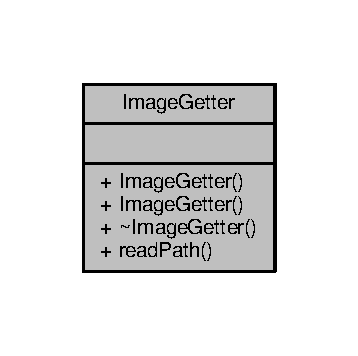
\includegraphics[width=172pt]{classImageGetter__coll__graph}
\end{center}
\end{figure}
\subsection*{Public Member Functions}
\begin{DoxyCompactItemize}
\item 
\hyperlink{classImageGetter_a799e38d342c813f0402310e1deaefff0}{Image\+Getter} ()
\item 
\hyperlink{classImageGetter_a4c302f858d6577426c1ec92ab2902675}{Image\+Getter} (const \hyperlink{classImageGetter}{Image\+Getter} \&orig)
\item 
virtual \hyperlink{classImageGetter_a7193a143aaddc4d82ed6f4901968dcc8}{$\sim$\+Image\+Getter} ()
\item 
void \hyperlink{classImageGetter_a92cd05c7e86df5bf83ee9f428a805fb3}{read\+Path} (std\+::vector$<$ std\+::string $>$ \&directiones, int \&cont, std\+::string path, int start\+Read, int end\+Read)
\end{DoxyCompactItemize}


\subsection{Constructor \& Destructor Documentation}
\index{Image\+Getter@{Image\+Getter}!Image\+Getter@{Image\+Getter}}
\index{Image\+Getter@{Image\+Getter}!Image\+Getter@{Image\+Getter}}
\subsubsection[{\texorpdfstring{Image\+Getter()}{ImageGetter()}}]{\setlength{\rightskip}{0pt plus 5cm}Image\+Getter\+::\+Image\+Getter (
\begin{DoxyParamCaption}
{}
\end{DoxyParamCaption}
)}\hypertarget{classImageGetter_a799e38d342c813f0402310e1deaefff0}{}\label{classImageGetter_a799e38d342c813f0402310e1deaefff0}

\begin{DoxyCode}
19                          \{
20 \}
\end{DoxyCode}
\index{Image\+Getter@{Image\+Getter}!Image\+Getter@{Image\+Getter}}
\index{Image\+Getter@{Image\+Getter}!Image\+Getter@{Image\+Getter}}
\subsubsection[{\texorpdfstring{Image\+Getter(const Image\+Getter \&orig)}{ImageGetter(const ImageGetter &orig)}}]{\setlength{\rightskip}{0pt plus 5cm}Image\+Getter\+::\+Image\+Getter (
\begin{DoxyParamCaption}
\item[{const {\bf Image\+Getter} \&}]{orig}
\end{DoxyParamCaption}
)}\hypertarget{classImageGetter_a4c302f858d6577426c1ec92ab2902675}{}\label{classImageGetter_a4c302f858d6577426c1ec92ab2902675}

\begin{DoxyCode}
22                                                 \{
23 \}
\end{DoxyCode}
\index{Image\+Getter@{Image\+Getter}!````~Image\+Getter@{$\sim$\+Image\+Getter}}
\index{````~Image\+Getter@{$\sim$\+Image\+Getter}!Image\+Getter@{Image\+Getter}}
\subsubsection[{\texorpdfstring{$\sim$\+Image\+Getter()}{~ImageGetter()}}]{\setlength{\rightskip}{0pt plus 5cm}Image\+Getter\+::$\sim$\+Image\+Getter (
\begin{DoxyParamCaption}
{}
\end{DoxyParamCaption}
)\hspace{0.3cm}{\ttfamily [virtual]}}\hypertarget{classImageGetter_a7193a143aaddc4d82ed6f4901968dcc8}{}\label{classImageGetter_a7193a143aaddc4d82ed6f4901968dcc8}

\begin{DoxyCode}
25                           \{
26 \}
\end{DoxyCode}


\subsection{Member Function Documentation}
\index{Image\+Getter@{Image\+Getter}!read\+Path@{read\+Path}}
\index{read\+Path@{read\+Path}!Image\+Getter@{Image\+Getter}}
\subsubsection[{\texorpdfstring{read\+Path(std\+::vector$<$ std\+::string $>$ \&directiones, int \&cont, std\+::string path, int start\+Read, int end\+Read)}{readPath(std::vector< std::string > &directiones, int &cont, std::string path, int startRead, int endRead)}}]{\setlength{\rightskip}{0pt plus 5cm}void Image\+Getter\+::read\+Path (
\begin{DoxyParamCaption}
\item[{std\+::vector$<$ std\+::string $>$ \&}]{directiones, }
\item[{int \&}]{cont, }
\item[{std\+::string}]{path, }
\item[{int}]{start\+Read, }
\item[{int}]{end\+Read}
\end{DoxyParamCaption}
)}\hypertarget{classImageGetter_a92cd05c7e86df5bf83ee9f428a805fb3}{}\label{classImageGetter_a92cd05c7e86df5bf83ee9f428a805fb3}
Funcion para leer el archivo que contiene la direccion de todas las imagenes en la base de datos 
\begin{DoxyParams}{Parameters}
{\em directiones} & \\
\hline
{\em cont} & \\
\hline
\end{DoxyParams}


Referenced by Image\+::generated\+Structure\+Shotton().


\begin{DoxyCode}
33                                                                                                            
              \{
34     std::ifstream file;
35     std::string line;
36     \textcolor{keywordtype}{int} numeroLinea = 0;
37     \textcolor{comment}{//int cont = 0;}
38     file.open(path.c\_str(), std::ifstream::in);
39     
40     \textcolor{comment}{//Leer el archivo hasta que termine.}
41     \textcolor{keywordflow}{while} (!file.eof()) \{
42         
43         \textcolor{keywordflow}{if}(numeroLinea >= startRead && numeroLinea<endRead)\{
44             getline(file, line); \textcolor{comment}{//Lee la linea}
45             directiones.push\_back(line); \textcolor{comment}{//agrega la linea al vector}
46         \}\textcolor{keywordflow}{else}\{
47             getline(file, line); \textcolor{comment}{//Lee la linea}
48         \}
49         \textcolor{keywordflow}{if}(numeroLinea == endRead)\{
50             \textcolor{keywordflow}{break};
51         \}
52         numeroLinea++;
53     \}
54     
55 
56     
57 \}\end{DoxyCode}


The documentation for this class was generated from the following files\+:\begin{DoxyCompactItemize}
\item 
\hyperlink{ImageGetter_8h}{Image\+Getter.\+h}\item 
\hyperlink{ImageGetter_8cpp}{Image\+Getter.\+cpp}\end{DoxyCompactItemize}

\hypertarget{classImageManager}{}\section{Image\+Manager Class Reference}
\label{classImageManager}\index{Image\+Manager@{Image\+Manager}}


{\ttfamily \#include $<$Image\+Manager.\+h$>$}



Collaboration diagram for Image\+Manager\+:
\nopagebreak
\begin{figure}[H]
\begin{center}
\leavevmode
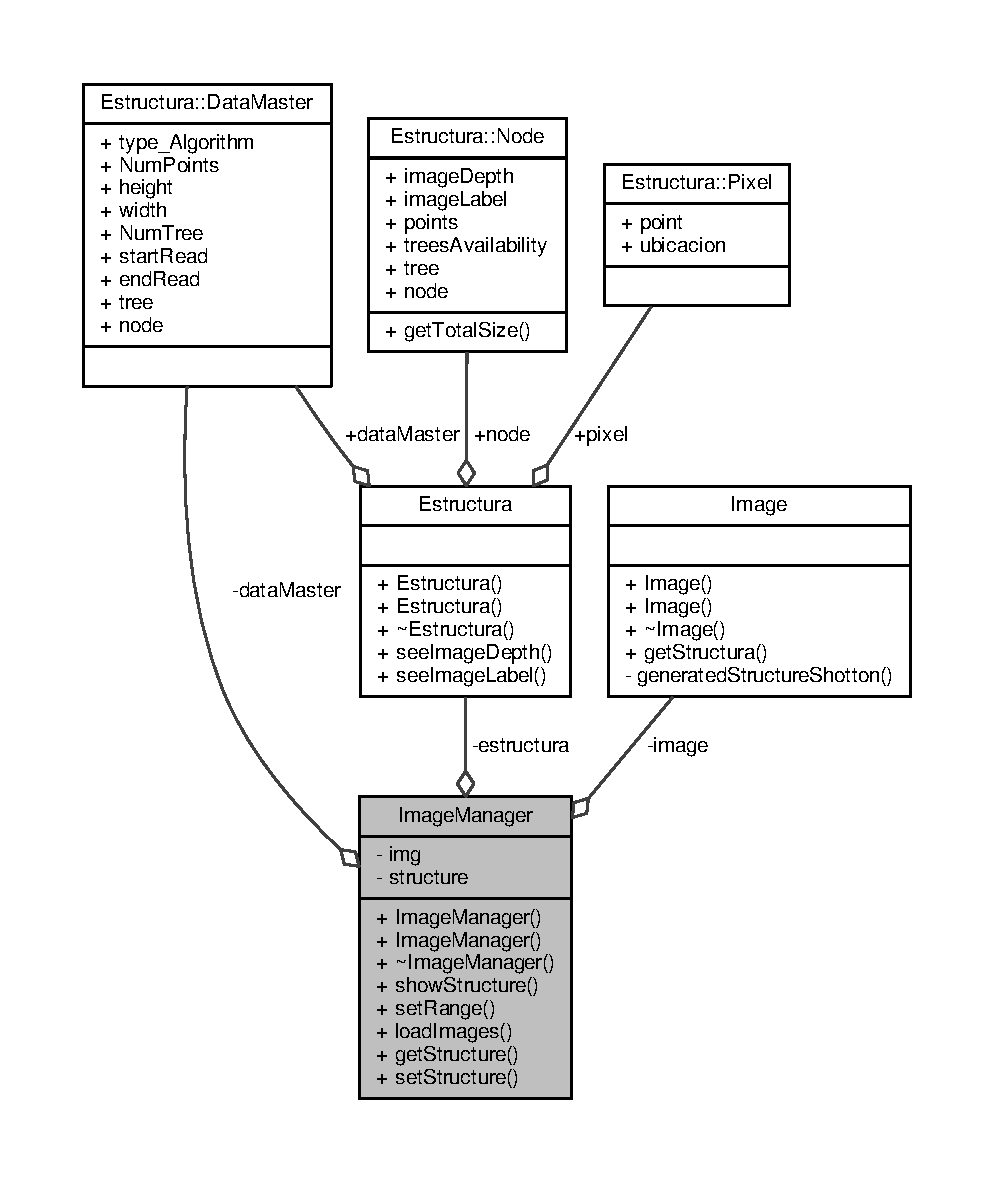
\includegraphics[width=350pt]{classImageManager__coll__graph}
\end{center}
\end{figure}
\subsection*{Public Member Functions}
\begin{DoxyCompactItemize}
\item 
\hyperlink{classImageManager_a8c856af0e3f0d23da7c765b0e33e585e}{Image\+Manager} ()
\item 
\hyperlink{classImageManager_a73c9c0419074956609f94dab2aacc183}{Image\+Manager} (const \hyperlink{classImageManager}{Image\+Manager} \&orig)
\item 
virtual \hyperlink{classImageManager_a3cad118fdf026d379641fb6b52cd1884}{$\sim$\+Image\+Manager} ()
\item 
void \hyperlink{classImageManager_a8b13aa8049b1294220d58b1c4749de9b}{show\+Structure} (bool show\+Images)
\item 
void \hyperlink{classImageManager_a21627e8230428f3a4bf7ec99703448e6}{set\+Range} (std\+::pair$<$ int, int $>$ p\+Range)
\item 
void \hyperlink{classImageManager_abbec13f7f949d5ea3b34fb52bd812e68}{load\+Images} ()
\item 
std\+::vector$<$ \hyperlink{structEstructura_1_1Node}{Estructura\+::\+Node} $>$ \hyperlink{classImageManager_adbdf00be4cb90cfb260cdc208612cd8c}{get\+Structure} () const 
\item 
void \hyperlink{classImageManager_ada142feb7f1f5e99a102ff043aacc6b7}{set\+Structure} (std\+::vector$<$ \hyperlink{structEstructura_1_1Node}{Estructura\+::\+Node} $>$ \hyperlink{classImageManager_a9a2da56c0a4aa3d4cdebdea45d81cca7}{structure})
\end{DoxyCompactItemize}
\subsection*{Private Attributes}
\begin{DoxyCompactItemize}
\item 
\hyperlink{classImage}{Image} \hyperlink{classImageManager_a8a66a77f0bb0dc06c2d3d064f9f1e27f}{image}
\item 
\hyperlink{classEstructura}{Estructura} \hyperlink{classImageManager_a9d328384bb5a1e13d0a50aefea3680cf}{estructura}
\item 
cv\+::\+Mat \hyperlink{classImageManager_ae096d2db43b8d7efe508ff68b987e992}{img}
\item 
std\+::vector$<$ \hyperlink{structEstructura_1_1Node}{Estructura\+::\+Node} $>$ \hyperlink{classImageManager_a9a2da56c0a4aa3d4cdebdea45d81cca7}{structure}
\item 
\hyperlink{structEstructura_1_1DataMaster}{Estructura\+::\+Data\+Master} \hyperlink{classImageManager_aa07e129af2fa348547c99843c0058c2b}{data\+Master}
\end{DoxyCompactItemize}


\subsection{Constructor \& Destructor Documentation}
\index{Image\+Manager@{Image\+Manager}!Image\+Manager@{Image\+Manager}}
\index{Image\+Manager@{Image\+Manager}!Image\+Manager@{Image\+Manager}}
\subsubsection[{\texorpdfstring{Image\+Manager()}{ImageManager()}}]{\setlength{\rightskip}{0pt plus 5cm}Image\+Manager\+::\+Image\+Manager (
\begin{DoxyParamCaption}
{}
\end{DoxyParamCaption}
)}\hypertarget{classImageManager_a8c856af0e3f0d23da7c765b0e33e585e}{}\label{classImageManager_a8c856af0e3f0d23da7c765b0e33e585e}


References data\+Master, Estructura\+::\+Data\+Master\+::height, Estructura\+::\+Data\+Master\+::node, Estructura\+::\+Data\+Master\+::\+Num\+Points, Estructura\+::\+Data\+Master\+::\+Num\+Tree, Estructura\+::\+Data\+Master\+::tree, Estructura\+::\+Data\+Master\+::type\+\_\+\+Algorithm, and Estructura\+::\+Data\+Master\+::width.


\begin{DoxyCode}
16                            \{
17     \hyperlink{classImageManager_aa07e129af2fa348547c99843c0058c2b}{dataMaster}.\hyperlink{structEstructura_1_1DataMaster_ad62760f62256a3fbd88481f720b81851}{NumPoints} = 15;
18     \hyperlink{classImageManager_aa07e129af2fa348547c99843c0058c2b}{dataMaster}.\hyperlink{structEstructura_1_1DataMaster_a33df1604c867e22af955f29c453d6651}{height} = 240;
19     \hyperlink{classImageManager_aa07e129af2fa348547c99843c0058c2b}{dataMaster}.\hyperlink{structEstructura_1_1DataMaster_a52e88b0d0d52d7e61880e3689ef2e638}{width} = 320;
20     \hyperlink{classImageManager_aa07e129af2fa348547c99843c0058c2b}{dataMaster}.\hyperlink{structEstructura_1_1DataMaster_a950938f474870649fe7eceae940366fd}{NumTree} = 3;
21     \hyperlink{classImageManager_aa07e129af2fa348547c99843c0058c2b}{dataMaster}.\hyperlink{structEstructura_1_1DataMaster_a766b1b437e0f242d3626a3759bef8b43}{tree} = 0;
22     \hyperlink{classImageManager_aa07e129af2fa348547c99843c0058c2b}{dataMaster}.\hyperlink{structEstructura_1_1DataMaster_a5b7bf8e1c983ad0a64dd596d1bb4e31a}{node} = 0;
23     \hyperlink{classImageManager_aa07e129af2fa348547c99843c0058c2b}{dataMaster}.\hyperlink{structEstructura_1_1DataMaster_accae7ba56def5fd845b33cb8cfb384fe}{type\_Algorithm} = \textcolor{stringliteral}{"shotton"};
24 \}
\end{DoxyCode}
\index{Image\+Manager@{Image\+Manager}!Image\+Manager@{Image\+Manager}}
\index{Image\+Manager@{Image\+Manager}!Image\+Manager@{Image\+Manager}}
\subsubsection[{\texorpdfstring{Image\+Manager(const Image\+Manager \&orig)}{ImageManager(const ImageManager &orig)}}]{\setlength{\rightskip}{0pt plus 5cm}Image\+Manager\+::\+Image\+Manager (
\begin{DoxyParamCaption}
\item[{const {\bf Image\+Manager} \&}]{orig}
\end{DoxyParamCaption}
)}\hypertarget{classImageManager_a73c9c0419074956609f94dab2aacc183}{}\label{classImageManager_a73c9c0419074956609f94dab2aacc183}

\begin{DoxyCode}
26                                                    \{
27 \}
\end{DoxyCode}
\index{Image\+Manager@{Image\+Manager}!````~Image\+Manager@{$\sim$\+Image\+Manager}}
\index{````~Image\+Manager@{$\sim$\+Image\+Manager}!Image\+Manager@{Image\+Manager}}
\subsubsection[{\texorpdfstring{$\sim$\+Image\+Manager()}{~ImageManager()}}]{\setlength{\rightskip}{0pt plus 5cm}Image\+Manager\+::$\sim$\+Image\+Manager (
\begin{DoxyParamCaption}
{}
\end{DoxyParamCaption}
)\hspace{0.3cm}{\ttfamily [virtual]}}\hypertarget{classImageManager_a3cad118fdf026d379641fb6b52cd1884}{}\label{classImageManager_a3cad118fdf026d379641fb6b52cd1884}

\begin{DoxyCode}
29                             \{
30 \}
\end{DoxyCode}


\subsection{Member Function Documentation}
\index{Image\+Manager@{Image\+Manager}!get\+Structure@{get\+Structure}}
\index{get\+Structure@{get\+Structure}!Image\+Manager@{Image\+Manager}}
\subsubsection[{\texorpdfstring{get\+Structure() const }{getStructure() const }}]{\setlength{\rightskip}{0pt plus 5cm}std\+::vector$<${\bf Estructura\+::\+Node}$>$ Image\+Manager\+::get\+Structure (
\begin{DoxyParamCaption}
{}
\end{DoxyParamCaption}
) const\hspace{0.3cm}{\ttfamily [inline]}}\hypertarget{classImageManager_adbdf00be4cb90cfb260cdc208612cd8c}{}\label{classImageManager_adbdf00be4cb90cfb260cdc208612cd8c}


References structure.


\begin{DoxyCode}
44                                                    \{
45         \textcolor{keywordflow}{return} \hyperlink{classImageManager_a9a2da56c0a4aa3d4cdebdea45d81cca7}{structure};
46     \}
\end{DoxyCode}
\index{Image\+Manager@{Image\+Manager}!load\+Images@{load\+Images}}
\index{load\+Images@{load\+Images}!Image\+Manager@{Image\+Manager}}
\subsubsection[{\texorpdfstring{load\+Images()}{loadImages()}}]{\setlength{\rightskip}{0pt plus 5cm}void Image\+Manager\+::load\+Images (
\begin{DoxyParamCaption}
{}
\end{DoxyParamCaption}
)}\hypertarget{classImageManager_abbec13f7f949d5ea3b34fb52bd812e68}{}\label{classImageManager_abbec13f7f949d5ea3b34fb52bd812e68}


References data\+Master, Image\+::get\+Structura(), image, and structure.



Referenced by rdf\+::\+Distribution\+Manager\+::transfer\+Ranges().


\begin{DoxyCode}
37                               \{
38     \hyperlink{classImageManager_a8a66a77f0bb0dc06c2d3d064f9f1e27f}{image}.\hyperlink{classImage_ad5ed787922c9c8aad26e1e349bdc4018}{getStructura}(\hyperlink{classImageManager_a9a2da56c0a4aa3d4cdebdea45d81cca7}{structure}, \hyperlink{classImageManager_aa07e129af2fa348547c99843c0058c2b}{dataMaster});
39     
40 \}
\end{DoxyCode}
\index{Image\+Manager@{Image\+Manager}!set\+Range@{set\+Range}}
\index{set\+Range@{set\+Range}!Image\+Manager@{Image\+Manager}}
\subsubsection[{\texorpdfstring{set\+Range(std\+::pair$<$ int, int $>$ p\+Range)}{setRange(std::pair< int, int > pRange)}}]{\setlength{\rightskip}{0pt plus 5cm}void Image\+Manager\+::set\+Range (
\begin{DoxyParamCaption}
\item[{std\+::pair$<$ int, int $>$}]{p\+Range}
\end{DoxyParamCaption}
)}\hypertarget{classImageManager_a21627e8230428f3a4bf7ec99703448e6}{}\label{classImageManager_a21627e8230428f3a4bf7ec99703448e6}


References data\+Master, Estructura\+::\+Data\+Master\+::end\+Read, and Estructura\+::\+Data\+Master\+::start\+Read.



Referenced by rdf\+::\+Distribution\+Manager\+::transfer\+Ranges().


\begin{DoxyCode}
32                                                     \{
33     \hyperlink{classImageManager_aa07e129af2fa348547c99843c0058c2b}{dataMaster}.\hyperlink{structEstructura_1_1DataMaster_ada49eb1401a3715858043ebd2b61c10c}{startRead} = pRange.first;
34     \hyperlink{classImageManager_aa07e129af2fa348547c99843c0058c2b}{dataMaster}.\hyperlink{structEstructura_1_1DataMaster_a787807eccc80c8e639d2409477f37f3a}{endRead} = pRange.second;
35 \}
\end{DoxyCode}
\index{Image\+Manager@{Image\+Manager}!set\+Structure@{set\+Structure}}
\index{set\+Structure@{set\+Structure}!Image\+Manager@{Image\+Manager}}
\subsubsection[{\texorpdfstring{set\+Structure(std\+::vector$<$ Estructura\+::\+Node $>$ structure)}{setStructure(std::vector< Estructura::Node > structure)}}]{\setlength{\rightskip}{0pt plus 5cm}void Image\+Manager\+::set\+Structure (
\begin{DoxyParamCaption}
\item[{std\+::vector$<$ {\bf Estructura\+::\+Node} $>$}]{structure}
\end{DoxyParamCaption}
)\hspace{0.3cm}{\ttfamily [inline]}}\hypertarget{classImageManager_ada142feb7f1f5e99a102ff043aacc6b7}{}\label{classImageManager_ada142feb7f1f5e99a102ff043aacc6b7}


References structure.


\begin{DoxyCode}
48                                                            \{
49         this->\hyperlink{classImageManager_a9a2da56c0a4aa3d4cdebdea45d81cca7}{structure} = \hyperlink{classImageManager_a9a2da56c0a4aa3d4cdebdea45d81cca7}{structure};
50     \}
\end{DoxyCode}
\index{Image\+Manager@{Image\+Manager}!show\+Structure@{show\+Structure}}
\index{show\+Structure@{show\+Structure}!Image\+Manager@{Image\+Manager}}
\subsubsection[{\texorpdfstring{show\+Structure(bool show\+Images)}{showStructure(bool showImages)}}]{\setlength{\rightskip}{0pt plus 5cm}void Image\+Manager\+::show\+Structure (
\begin{DoxyParamCaption}
\item[{bool}]{show\+Images}
\end{DoxyParamCaption}
)}\hypertarget{classImageManager_a8b13aa8049b1294220d58b1c4749de9b}{}\label{classImageManager_a8b13aa8049b1294220d58b1c4749de9b}


References estructura, img, Estructura\+::see\+Image\+Depth(), Estructura\+::see\+Image\+Label(), and structure.


\begin{DoxyCode}
42                                                 \{
43     \textcolor{comment}{//desmostracion de la estructura esta bien}
44     \textcolor{keywordflow}{for} (\textcolor{keywordtype}{int} i = 0; i < \hyperlink{classImageManager_a9a2da56c0a4aa3d4cdebdea45d81cca7}{structure}.size(); i++) \{
45         \hyperlink{classImageManager_ae096d2db43b8d7efe508ff68b987e992}{img} = \hyperlink{classImageManager_a9a2da56c0a4aa3d4cdebdea45d81cca7}{structure}[i].imageLabel;  
46         std::vector<Estructura::Pixel> pixel = \hyperlink{classImageManager_a9a2da56c0a4aa3d4cdebdea45d81cca7}{structure}[i].points; 
47         \textcolor{keywordflow}{if}(showImages)\{
48             \hyperlink{classImageManager_a9d328384bb5a1e13d0a50aefea3680cf}{estructura}.\hyperlink{classEstructura_a4d6f678e0c5a5f2df96b50064304eec1}{seeImageLabel}(\hyperlink{classImageManager_ae096d2db43b8d7efe508ff68b987e992}{img});
49             \hyperlink{classImageManager_a9d328384bb5a1e13d0a50aefea3680cf}{estructura}.\hyperlink{classEstructura_a64b30b9326081ddd31ea330c4036cf5a}{seeImageDepth}(240,320,\hyperlink{classImageManager_ae096d2db43b8d7efe508ff68b987e992}{img});
50         \}
51         \textcolor{keywordflow}{else} \{
52             \textcolor{keywordflow}{for} (\textcolor{keywordtype}{int} j = 0; j < pixel.size(); j++) \{
53                 std::cout <<  pixel[j].point<< \textcolor{stringliteral}{"\(\backslash\)n"};
54             \}
55         \}    
56     \}
57 \}
\end{DoxyCode}


\subsection{Member Data Documentation}
\index{Image\+Manager@{Image\+Manager}!data\+Master@{data\+Master}}
\index{data\+Master@{data\+Master}!Image\+Manager@{Image\+Manager}}
\subsubsection[{\texorpdfstring{data\+Master}{dataMaster}}]{\setlength{\rightskip}{0pt plus 5cm}{\bf Estructura\+::\+Data\+Master} Image\+Manager\+::data\+Master\hspace{0.3cm}{\ttfamily [private]}}\hypertarget{classImageManager_aa07e129af2fa348547c99843c0058c2b}{}\label{classImageManager_aa07e129af2fa348547c99843c0058c2b}


Referenced by Image\+Manager(), load\+Images(), and set\+Range().

\index{Image\+Manager@{Image\+Manager}!estructura@{estructura}}
\index{estructura@{estructura}!Image\+Manager@{Image\+Manager}}
\subsubsection[{\texorpdfstring{estructura}{estructura}}]{\setlength{\rightskip}{0pt plus 5cm}{\bf Estructura} Image\+Manager\+::estructura\hspace{0.3cm}{\ttfamily [private]}}\hypertarget{classImageManager_a9d328384bb5a1e13d0a50aefea3680cf}{}\label{classImageManager_a9d328384bb5a1e13d0a50aefea3680cf}


Referenced by show\+Structure().

\index{Image\+Manager@{Image\+Manager}!image@{image}}
\index{image@{image}!Image\+Manager@{Image\+Manager}}
\subsubsection[{\texorpdfstring{image}{image}}]{\setlength{\rightskip}{0pt plus 5cm}{\bf Image} Image\+Manager\+::image\hspace{0.3cm}{\ttfamily [private]}}\hypertarget{classImageManager_a8a66a77f0bb0dc06c2d3d064f9f1e27f}{}\label{classImageManager_a8a66a77f0bb0dc06c2d3d064f9f1e27f}


Referenced by load\+Images().

\index{Image\+Manager@{Image\+Manager}!img@{img}}
\index{img@{img}!Image\+Manager@{Image\+Manager}}
\subsubsection[{\texorpdfstring{img}{img}}]{\setlength{\rightskip}{0pt plus 5cm}cv\+::\+Mat Image\+Manager\+::img\hspace{0.3cm}{\ttfamily [private]}}\hypertarget{classImageManager_ae096d2db43b8d7efe508ff68b987e992}{}\label{classImageManager_ae096d2db43b8d7efe508ff68b987e992}


Referenced by show\+Structure().

\index{Image\+Manager@{Image\+Manager}!structure@{structure}}
\index{structure@{structure}!Image\+Manager@{Image\+Manager}}
\subsubsection[{\texorpdfstring{structure}{structure}}]{\setlength{\rightskip}{0pt plus 5cm}std\+::vector$<${\bf Estructura\+::\+Node}$>$ Image\+Manager\+::structure\hspace{0.3cm}{\ttfamily [private]}}\hypertarget{classImageManager_a9a2da56c0a4aa3d4cdebdea45d81cca7}{}\label{classImageManager_a9a2da56c0a4aa3d4cdebdea45d81cca7}


Referenced by get\+Structure(), load\+Images(), set\+Structure(), and show\+Structure().



The documentation for this class was generated from the following files\+:\begin{DoxyCompactItemize}
\item 
\hyperlink{ImageManager_8h}{Image\+Manager.\+h}\item 
\hyperlink{ImageManager_8cpp}{Image\+Manager.\+cpp}\end{DoxyCompactItemize}

\hypertarget{classrdf_1_1ImageOperations}{}\section{rdf\+:\+:Image\+Operations Class Reference}
\label{classrdf_1_1ImageOperations}\index{rdf\+::\+Image\+Operations@{rdf\+::\+Image\+Operations}}


{\ttfamily \#include $<$Image\+Operations.\+h$>$}



Collaboration diagram for rdf\+:\+:Image\+Operations\+:
\nopagebreak
\begin{figure}[H]
\begin{center}
\leavevmode
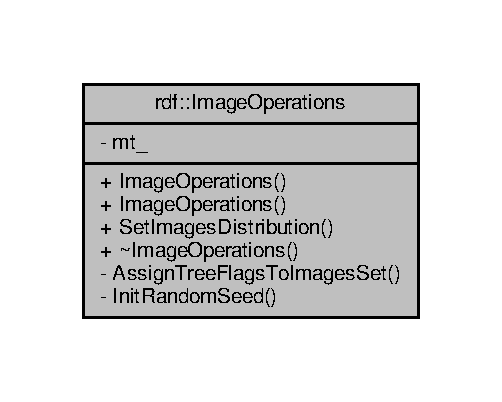
\includegraphics[width=241pt]{classrdf_1_1ImageOperations__coll__graph}
\end{center}
\end{figure}
\subsection*{Public Member Functions}
\begin{DoxyCompactItemize}
\item 
\hyperlink{classrdf_1_1ImageOperations_aa002ef8c8043e4bcff91058206dfa2fd}{Image\+Operations} ()
\item 
\hyperlink{classrdf_1_1ImageOperations_ab125b701dc20455468305ff1c71e33e9}{Image\+Operations} (const \hyperlink{classrdf_1_1ImageOperations}{Image\+Operations} \&orig)
\item 
void \hyperlink{classrdf_1_1ImageOperations_a0058a30a2dc6063bc60ce893fd714b10}{Set\+Images\+Distribution} (std\+::vector$<$ \hyperlink{structEstructura_1_1Node}{Estructura\+::\+Node} $>$ \&, int, int)
\item 
virtual \hyperlink{classrdf_1_1ImageOperations_a12ddf1b0e39dc483d20273123fdf6b06}{$\sim$\+Image\+Operations} ()
\end{DoxyCompactItemize}
\subsection*{Private Member Functions}
\begin{DoxyCompactItemize}
\item 
void \hyperlink{classrdf_1_1ImageOperations_ab1b9ee966da291117ba9ba1a82da99e2}{Assign\+Tree\+Flags\+To\+Images\+Set} (std\+::vector$<$ \hyperlink{structEstructura_1_1Node}{Estructura\+::\+Node} $>$ \&, int, int, int)
\end{DoxyCompactItemize}
\subsection*{Static Private Member Functions}
\begin{DoxyCompactItemize}
\item 
static std\+::mt19937 \hyperlink{classrdf_1_1ImageOperations_a03c4b3974a08a143dbce967cae91498f}{Init\+Random\+Seed} ()
\end{DoxyCompactItemize}
\subsection*{Static Private Attributes}
\begin{DoxyCompactItemize}
\item 
static std\+::mt19937 \hyperlink{classrdf_1_1ImageOperations_a84569ca7efeca0cc3d0024e36f841d37}{mt\+\_\+} = \hyperlink{classrdf_1_1ImageOperations_a03c4b3974a08a143dbce967cae91498f}{Image\+Operations\+::\+Init\+Random\+Seed}()
\end{DoxyCompactItemize}


\subsection{Constructor \& Destructor Documentation}
\index{rdf\+::\+Image\+Operations@{rdf\+::\+Image\+Operations}!Image\+Operations@{Image\+Operations}}
\index{Image\+Operations@{Image\+Operations}!rdf\+::\+Image\+Operations@{rdf\+::\+Image\+Operations}}
\subsubsection[{\texorpdfstring{Image\+Operations()}{ImageOperations()}}]{\setlength{\rightskip}{0pt plus 5cm}Image\+Operations\+::\+Image\+Operations (
\begin{DoxyParamCaption}
{}
\end{DoxyParamCaption}
)}\hypertarget{classrdf_1_1ImageOperations_aa002ef8c8043e4bcff91058206dfa2fd}{}\label{classrdf_1_1ImageOperations_aa002ef8c8043e4bcff91058206dfa2fd}

\begin{DoxyCode}
29                                  \{
30 \}
\end{DoxyCode}
\index{rdf\+::\+Image\+Operations@{rdf\+::\+Image\+Operations}!Image\+Operations@{Image\+Operations}}
\index{Image\+Operations@{Image\+Operations}!rdf\+::\+Image\+Operations@{rdf\+::\+Image\+Operations}}
\subsubsection[{\texorpdfstring{Image\+Operations(const Image\+Operations \&orig)}{ImageOperations(const ImageOperations &orig)}}]{\setlength{\rightskip}{0pt plus 5cm}Image\+Operations\+::\+Image\+Operations (
\begin{DoxyParamCaption}
\item[{const {\bf Image\+Operations} \&}]{orig}
\end{DoxyParamCaption}
)}\hypertarget{classrdf_1_1ImageOperations_ab125b701dc20455468305ff1c71e33e9}{}\label{classrdf_1_1ImageOperations_ab125b701dc20455468305ff1c71e33e9}

\begin{DoxyCode}
32                                                             \{
33 \}
\end{DoxyCode}
\index{rdf\+::\+Image\+Operations@{rdf\+::\+Image\+Operations}!````~Image\+Operations@{$\sim$\+Image\+Operations}}
\index{````~Image\+Operations@{$\sim$\+Image\+Operations}!rdf\+::\+Image\+Operations@{rdf\+::\+Image\+Operations}}
\subsubsection[{\texorpdfstring{$\sim$\+Image\+Operations()}{~ImageOperations()}}]{\setlength{\rightskip}{0pt plus 5cm}Image\+Operations\+::$\sim$\+Image\+Operations (
\begin{DoxyParamCaption}
{}
\end{DoxyParamCaption}
)\hspace{0.3cm}{\ttfamily [virtual]}}\hypertarget{classrdf_1_1ImageOperations_a12ddf1b0e39dc483d20273123fdf6b06}{}\label{classrdf_1_1ImageOperations_a12ddf1b0e39dc483d20273123fdf6b06}

\begin{DoxyCode}
72                                   \{
73 \}
\end{DoxyCode}


\subsection{Member Function Documentation}
\index{rdf\+::\+Image\+Operations@{rdf\+::\+Image\+Operations}!Assign\+Tree\+Flags\+To\+Images\+Set@{Assign\+Tree\+Flags\+To\+Images\+Set}}
\index{Assign\+Tree\+Flags\+To\+Images\+Set@{Assign\+Tree\+Flags\+To\+Images\+Set}!rdf\+::\+Image\+Operations@{rdf\+::\+Image\+Operations}}
\subsubsection[{\texorpdfstring{Assign\+Tree\+Flags\+To\+Images\+Set(std\+::vector$<$ Estructura\+::\+Node $>$ \&, int, int, int)}{AssignTreeFlagsToImagesSet(std::vector< Estructura::Node > &, int, int, int)}}]{\setlength{\rightskip}{0pt plus 5cm}void Image\+Operations\+::\+Assign\+Tree\+Flags\+To\+Images\+Set (
\begin{DoxyParamCaption}
\item[{std\+::vector$<$ {\bf Estructura\+::\+Node} $>$ \&}]{images\+Set, }
\item[{int}]{percentage\+Num, }
\item[{int}]{tree\+Num, }
\item[{int}]{total\+Size}
\end{DoxyParamCaption}
)\hspace{0.3cm}{\ttfamily [private]}}\hypertarget{classrdf_1_1ImageOperations_ab1b9ee966da291117ba9ba1a82da99e2}{}\label{classrdf_1_1ImageOperations_ab1b9ee966da291117ba9ba1a82da99e2}


References mt\+\_\+.



Referenced by Set\+Images\+Distribution().


\begin{DoxyCode}
53  \{
54     \textcolor{keywordtype}{int} count = 0;
55     \textcolor{keywordtype}{int} randomNum = 0;
56     \textcolor{keywordtype}{int} treeFlag = 0;
57     std::uniform\_int\_distribution<int> int\_dist(0, totalSize - 1);
58     \textcolor{keywordflow}{while} (count < percentageNum) \{
59       randomNum = int\_dist(\hyperlink{classrdf_1_1ImageOperations_a84569ca7efeca0cc3d0024e36f841d37}{mt\_});
60       treeFlag = imagesSet[randomNum].treesAvailability[treeNum];
61       \textcolor{keywordflow}{if} (treeFlag == 0)\{
62         imagesSet[randomNum].treesAvailability[treeNum] = 1;
63         count++;
64       \}
65     \}
66   \}
\end{DoxyCode}
\index{rdf\+::\+Image\+Operations@{rdf\+::\+Image\+Operations}!Init\+Random\+Seed@{Init\+Random\+Seed}}
\index{Init\+Random\+Seed@{Init\+Random\+Seed}!rdf\+::\+Image\+Operations@{rdf\+::\+Image\+Operations}}
\subsubsection[{\texorpdfstring{Init\+Random\+Seed()}{InitRandomSeed()}}]{\setlength{\rightskip}{0pt plus 5cm}std\+::mt19937 Image\+Operations\+::\+Init\+Random\+Seed (
\begin{DoxyParamCaption}
{}
\end{DoxyParamCaption}
)\hspace{0.3cm}{\ttfamily [static]}, {\ttfamily [private]}}\hypertarget{classrdf_1_1ImageOperations_a03c4b3974a08a143dbce967cae91498f}{}\label{classrdf_1_1ImageOperations_a03c4b3974a08a143dbce967cae91498f}


References mt\+\_\+.


\begin{DoxyCode}
77                                            \{
78     std::random\_device rd;
79     std::mt19937 mt(rd());
80     \textcolor{keywordflow}{return} mt;
81 \}
\end{DoxyCode}
\index{rdf\+::\+Image\+Operations@{rdf\+::\+Image\+Operations}!Set\+Images\+Distribution@{Set\+Images\+Distribution}}
\index{Set\+Images\+Distribution@{Set\+Images\+Distribution}!rdf\+::\+Image\+Operations@{rdf\+::\+Image\+Operations}}
\subsubsection[{\texorpdfstring{Set\+Images\+Distribution(std\+::vector$<$ Estructura\+::\+Node $>$ \&, int, int)}{SetImagesDistribution(std::vector< Estructura::Node > &, int, int)}}]{\setlength{\rightskip}{0pt plus 5cm}void Image\+Operations\+::\+Set\+Images\+Distribution (
\begin{DoxyParamCaption}
\item[{std\+::vector$<$ {\bf Estructura\+::\+Node} $>$ \&}]{images\+Set, }
\item[{int}]{percentage, }
\item[{int}]{num\+Trees}
\end{DoxyParamCaption}
)}\hypertarget{classrdf_1_1ImageOperations_a0058a30a2dc6063bc60ce893fd714b10}{}\label{classrdf_1_1ImageOperations_a0058a30a2dc6063bc60ce893fd714b10}


References Assign\+Tree\+Flags\+To\+Images\+Set().


\begin{DoxyCode}
40  \{
41     \textcolor{keywordtype}{int} total = imagesSet.size();
42     \textcolor{keywordtype}{int} percentageNum = (percentage / 100) * total;
43     \textcolor{keywordflow}{for} (\textcolor{keywordtype}{int} i = 0; i < numTrees; i++) \{
44       \hyperlink{classrdf_1_1ImageOperations_ab1b9ee966da291117ba9ba1a82da99e2}{AssignTreeFlagsToImagesSet}(imagesSet, percentageNum, i, total);
45     \}
46 \}
\end{DoxyCode}


\subsection{Member Data Documentation}
\index{rdf\+::\+Image\+Operations@{rdf\+::\+Image\+Operations}!mt\+\_\+@{mt\+\_\+}}
\index{mt\+\_\+@{mt\+\_\+}!rdf\+::\+Image\+Operations@{rdf\+::\+Image\+Operations}}
\subsubsection[{\texorpdfstring{mt\+\_\+}{mt_}}]{\setlength{\rightskip}{0pt plus 5cm}std\+::mt19937 Image\+Operations\+::mt\+\_\+ = {\bf Image\+Operations\+::\+Init\+Random\+Seed}()\hspace{0.3cm}{\ttfamily [static]}, {\ttfamily [private]}}\hypertarget{classrdf_1_1ImageOperations_a84569ca7efeca0cc3d0024e36f841d37}{}\label{classrdf_1_1ImageOperations_a84569ca7efeca0cc3d0024e36f841d37}


Referenced by Assign\+Tree\+Flags\+To\+Images\+Set(), and Init\+Random\+Seed().



The documentation for this class was generated from the following files\+:\begin{DoxyCompactItemize}
\item 
\hyperlink{ImageOperations_8h}{Image\+Operations.\+h}\item 
\hyperlink{ImageOperations_8cpp}{Image\+Operations.\+cpp}\end{DoxyCompactItemize}

\hypertarget{classrdf_1_1Initializator}{}\section{rdf\+:\+:Initializator Class Reference}
\label{classrdf_1_1Initializator}\index{rdf\+::\+Initializator@{rdf\+::\+Initializator}}


{\ttfamily \#include $<$Initializator.\+h$>$}



Collaboration diagram for rdf\+:\+:Initializator\+:
\nopagebreak
\begin{figure}[H]
\begin{center}
\leavevmode
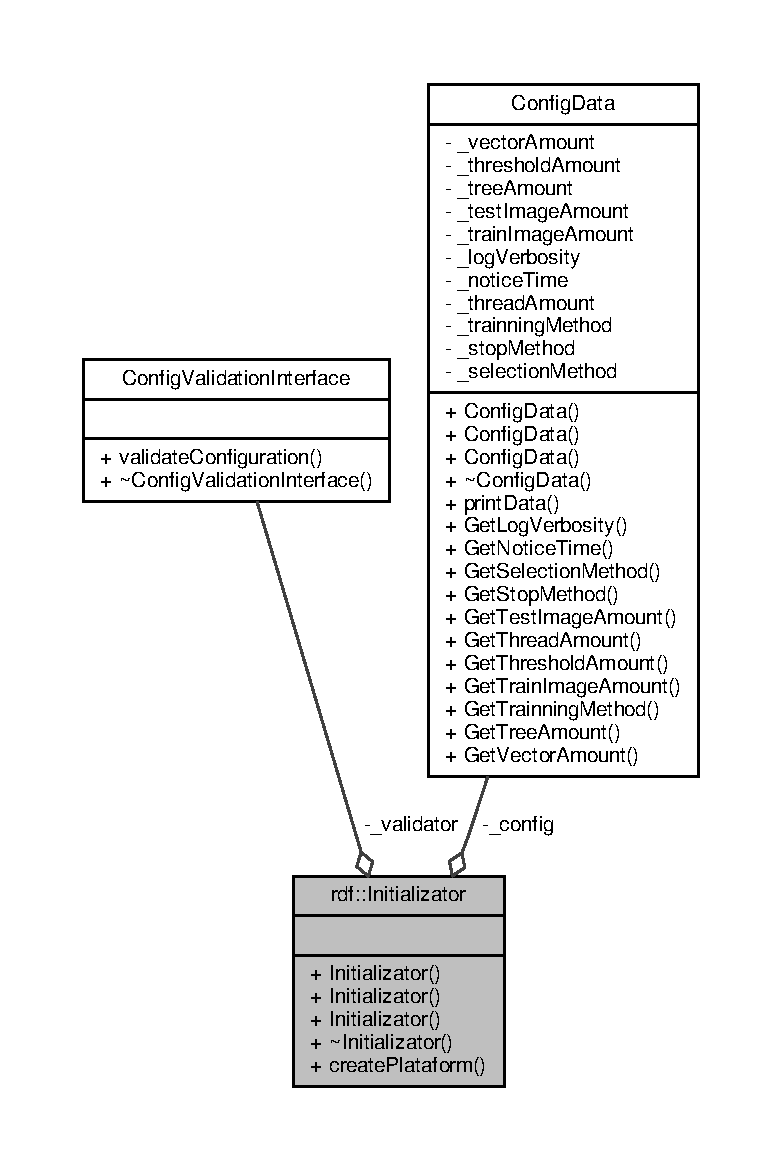
\includegraphics[width=350pt]{classrdf_1_1Initializator__coll__graph}
\end{center}
\end{figure}
\subsection*{Public Member Functions}
\begin{DoxyCompactItemize}
\item 
\hyperlink{classrdf_1_1Initializator_a0b3af95b92279e6fa09ebd629b6e3058}{Initializator} ()
\item 
\hyperlink{classrdf_1_1Initializator_ade9d2861f25524b5456482d8c504bdb5}{Initializator} (const \hyperlink{classrdf_1_1Initializator}{Initializator} \&orig)
\item 
\hyperlink{classrdf_1_1Initializator_aafbadfcb6826d7239681cf62d35adfa1}{Initializator} (const \hyperlink{classConfigData}{Config\+Data} \&Data)
\item 
virtual \hyperlink{classrdf_1_1Initializator_a49dcff8b25770c154fef04a9fead85b4}{$\sim$\+Initializator} ()
\item 
void \hyperlink{classrdf_1_1Initializator_ae48962e4dda1d9fff4bb1a9e1947fa9e}{create\+Plataform} ()
\end{DoxyCompactItemize}
\subsection*{Private Attributes}
\begin{DoxyCompactItemize}
\item 
\hyperlink{classConfigData}{Config\+Data} $\ast$ \hyperlink{classrdf_1_1Initializator_a5294154934886ac4dd76c4f808781cad}{\+\_\+config}
\item 
\hyperlink{classConfigValidationInterface}{Config\+Validation\+Interface} $\ast$ \hyperlink{classrdf_1_1Initializator_a961484bb3a4e149498fd093e395de9e4}{\+\_\+validator}
\end{DoxyCompactItemize}


\subsection{Constructor \& Destructor Documentation}
\index{rdf\+::\+Initializator@{rdf\+::\+Initializator}!Initializator@{Initializator}}
\index{Initializator@{Initializator}!rdf\+::\+Initializator@{rdf\+::\+Initializator}}
\subsubsection[{\texorpdfstring{Initializator()}{Initializator()}}]{\setlength{\rightskip}{0pt plus 5cm}rdf\+::\+Initializator\+::\+Initializator (
\begin{DoxyParamCaption}
{}
\end{DoxyParamCaption}
)}\hypertarget{classrdf_1_1Initializator_a0b3af95b92279e6fa09ebd629b6e3058}{}\label{classrdf_1_1Initializator_a0b3af95b92279e6fa09ebd629b6e3058}


References \+\_\+config, \+\_\+validator, L\+O\+G\+\_\+\+V\+E\+R\+B\+O\+S\+I\+TY, N\+O\+T\+I\+C\+E\+D\+\_\+\+T\+I\+ME, P\+R\+O\+C\+E\+S\+S\+\_\+\+A\+M\+O\+U\+NT, S\+E\+L\+E\+C\+T\+I\+O\+N\+\_\+\+M\+E\+T\+H\+OD, S\+T\+O\+P\+\_\+\+M\+E\+T\+H\+OD, T\+E\+S\+T\+\_\+\+I\+M\+A\+G\+E\+S\+\_\+\+A\+M\+O\+U\+NT, T\+H\+R\+E\+S\+H\+O\+L\+D\+\_\+\+A\+M\+O\+U\+NT, T\+R\+A\+I\+N\+\_\+\+I\+M\+A\+G\+E\+S\+\_\+\+A\+M\+O\+U\+NT, T\+R\+A\+I\+N\+N\+I\+N\+G\+\_\+\+M\+E\+T\+H\+OD, T\+R\+E\+E\+\_\+\+A\+M\+O\+U\+NT, and V\+E\+C\+T\+O\+R\+\_\+\+A\+M\+O\+U\+NT.


\begin{DoxyCode}
16                                 \{
17     \hyperlink{classrdf_1_1Initializator_a5294154934886ac4dd76c4f808781cad}{\_config} = \textcolor{keyword}{new} \hyperlink{classConfigData}{ConfigData}(       \hyperlink{Config_8h_a42a88b6f9794602ba8d3df8681586d6c}{VECTOR\_AMOUNT},
18                                 \hyperlink{Config_8h_a046baffcfc17bd9008df03cf43da388a}{THRESHOLD\_AMOUNT},
19                                 \hyperlink{Config_8h_a534cdc6cb39fa1f6fc95a92491cab5fb}{TREE\_AMOUNT}, 
20                                 \hyperlink{Config_8h_a8d13e9cc2082061ecb8db36a3f697964}{PROCESS\_AMOUNT}, 
21                                 \hyperlink{Config_8h_a2b708e4320618c29fd29d98d666e29f5}{TEST\_IMAGES\_AMOUNT},
22                                 \hyperlink{Config_8h_a2f82dae94103cd6733842f0fed0aeb62}{TRAIN\_IMAGES\_AMOUNT},
23                                 \hyperlink{Config_8h_a65533daa2b934c9fb36258439bdbcc4f}{LOG\_VERBOSITY},
24                                 \hyperlink{Config_8h_a31424dcd5dc3fdf15bde25f9d5963dd1}{NOTICED\_TIME},
25                                 \hyperlink{Config_8h_aaed4c456b4e56636c56d188849f8ddad}{TRAINNING\_METHOD}, 
26                                 \hyperlink{Config_8h_a784d3494097313752a8140763b84666e}{STOP\_METHOD}, 
27                                 \hyperlink{Config_8h_a07af8d3f8ee59b6ff02555bd154f3dbb}{SELECTION\_METHOD});
28     \hyperlink{classrdf_1_1Initializator_a961484bb3a4e149498fd093e395de9e4}{\_validator} = \textcolor{keyword}{new} \hyperlink{classuserValidator}{userValidator}(); 
29 \}
\end{DoxyCode}
\index{rdf\+::\+Initializator@{rdf\+::\+Initializator}!Initializator@{Initializator}}
\index{Initializator@{Initializator}!rdf\+::\+Initializator@{rdf\+::\+Initializator}}
\subsubsection[{\texorpdfstring{Initializator(const Initializator \&orig)}{Initializator(const Initializator &orig)}}]{\setlength{\rightskip}{0pt plus 5cm}rdf\+::\+Initializator\+::\+Initializator (
\begin{DoxyParamCaption}
\item[{const {\bf Initializator} \&}]{orig}
\end{DoxyParamCaption}
)}\hypertarget{classrdf_1_1Initializator_ade9d2861f25524b5456482d8c504bdb5}{}\label{classrdf_1_1Initializator_ade9d2861f25524b5456482d8c504bdb5}

\begin{DoxyCode}
31                                                          \{
32 \}
\end{DoxyCode}
\index{rdf\+::\+Initializator@{rdf\+::\+Initializator}!Initializator@{Initializator}}
\index{Initializator@{Initializator}!rdf\+::\+Initializator@{rdf\+::\+Initializator}}
\subsubsection[{\texorpdfstring{Initializator(const Config\+Data \&\+Data)}{Initializator(const ConfigData &Data)}}]{\setlength{\rightskip}{0pt plus 5cm}rdf\+::\+Initializator\+::\+Initializator (
\begin{DoxyParamCaption}
\item[{const {\bf Config\+Data} \&}]{Data}
\end{DoxyParamCaption}
)}\hypertarget{classrdf_1_1Initializator_aafbadfcb6826d7239681cf62d35adfa1}{}\label{classrdf_1_1Initializator_aafbadfcb6826d7239681cf62d35adfa1}
\index{rdf\+::\+Initializator@{rdf\+::\+Initializator}!````~Initializator@{$\sim$\+Initializator}}
\index{````~Initializator@{$\sim$\+Initializator}!rdf\+::\+Initializator@{rdf\+::\+Initializator}}
\subsubsection[{\texorpdfstring{$\sim$\+Initializator()}{~Initializator()}}]{\setlength{\rightskip}{0pt plus 5cm}rdf\+::\+Initializator\+::$\sim$\+Initializator (
\begin{DoxyParamCaption}
{}
\end{DoxyParamCaption}
)\hspace{0.3cm}{\ttfamily [virtual]}}\hypertarget{classrdf_1_1Initializator_a49dcff8b25770c154fef04a9fead85b4}{}\label{classrdf_1_1Initializator_a49dcff8b25770c154fef04a9fead85b4}

\begin{DoxyCode}
43                                  \{
44 \}
\end{DoxyCode}


\subsection{Member Function Documentation}
\index{rdf\+::\+Initializator@{rdf\+::\+Initializator}!create\+Plataform@{create\+Plataform}}
\index{create\+Plataform@{create\+Plataform}!rdf\+::\+Initializator@{rdf\+::\+Initializator}}
\subsubsection[{\texorpdfstring{create\+Plataform()}{createPlataform()}}]{\setlength{\rightskip}{0pt plus 5cm}void rdf\+::\+Initializator\+::create\+Plataform (
\begin{DoxyParamCaption}
{}
\end{DoxyParamCaption}
)}\hypertarget{classrdf_1_1Initializator_ae48962e4dda1d9fff4bb1a9e1947fa9e}{}\label{classrdf_1_1Initializator_ae48962e4dda1d9fff4bb1a9e1947fa9e}


References \+\_\+config, \+\_\+validator, and Config\+Validation\+Interface\+::validate\+Configuration().



Referenced by rdf\+::\+Train\+Manager\+::validate\+Configuration().


\begin{DoxyCode}
34                                       \{
35     \textcolor{keywordflow}{if}(\hyperlink{classrdf_1_1Initializator_a961484bb3a4e149498fd093e395de9e4}{\_validator}->\hyperlink{classConfigValidationInterface_a9f500c653a7b4b4559f920d499d7b96d}{validateConfiguration}(*\hyperlink{classrdf_1_1Initializator_a5294154934886ac4dd76c4f808781cad}{\_config}))\{
36         cout << \textcolor{stringliteral}{"Creating Plataform \(\backslash\)n"};
37     \}
38     \textcolor{keywordflow}{else} \{
39         cout << \textcolor{stringliteral}{"Error creating Plataform \(\backslash\)n"};
40     \}
41 \}
\end{DoxyCode}


\subsection{Member Data Documentation}
\index{rdf\+::\+Initializator@{rdf\+::\+Initializator}!\+\_\+config@{\+\_\+config}}
\index{\+\_\+config@{\+\_\+config}!rdf\+::\+Initializator@{rdf\+::\+Initializator}}
\subsubsection[{\texorpdfstring{\+\_\+config}{_config}}]{\setlength{\rightskip}{0pt plus 5cm}{\bf Config\+Data}$\ast$ rdf\+::\+Initializator\+::\+\_\+config\hspace{0.3cm}{\ttfamily [private]}}\hypertarget{classrdf_1_1Initializator_a5294154934886ac4dd76c4f808781cad}{}\label{classrdf_1_1Initializator_a5294154934886ac4dd76c4f808781cad}


Referenced by create\+Plataform(), and Initializator().

\index{rdf\+::\+Initializator@{rdf\+::\+Initializator}!\+\_\+validator@{\+\_\+validator}}
\index{\+\_\+validator@{\+\_\+validator}!rdf\+::\+Initializator@{rdf\+::\+Initializator}}
\subsubsection[{\texorpdfstring{\+\_\+validator}{_validator}}]{\setlength{\rightskip}{0pt plus 5cm}{\bf Config\+Validation\+Interface}$\ast$ rdf\+::\+Initializator\+::\+\_\+validator\hspace{0.3cm}{\ttfamily [private]}}\hypertarget{classrdf_1_1Initializator_a961484bb3a4e149498fd093e395de9e4}{}\label{classrdf_1_1Initializator_a961484bb3a4e149498fd093e395de9e4}


Referenced by create\+Plataform(), and Initializator().



The documentation for this class was generated from the following files\+:\begin{DoxyCompactItemize}
\item 
\hyperlink{Initializator_8h}{Initializator.\+h}\item 
\hyperlink{Initializator_8cpp}{Initializator.\+cpp}\end{DoxyCompactItemize}

\hypertarget{classLabelImage}{}\section{Label\+Image Class Reference}
\label{classLabelImage}\index{Label\+Image@{Label\+Image}}


{\ttfamily \#include $<$Label\+Image.\+h$>$}



Inheritance diagram for Label\+Image\+:
\nopagebreak
\begin{figure}[H]
\begin{center}
\leavevmode
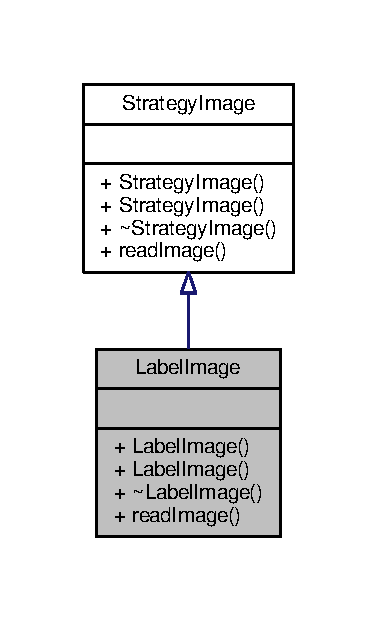
\includegraphics[width=181pt]{classLabelImage__inherit__graph}
\end{center}
\end{figure}


Collaboration diagram for Label\+Image\+:
\nopagebreak
\begin{figure}[H]
\begin{center}
\leavevmode
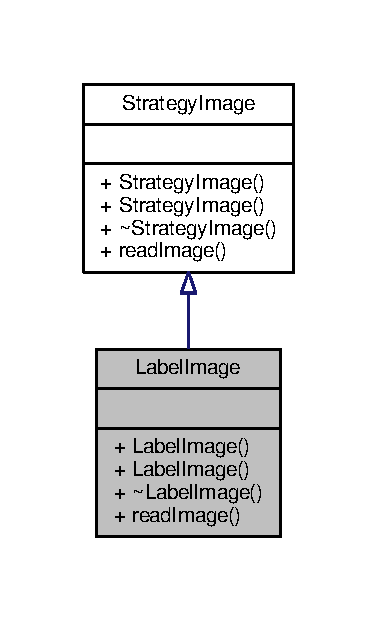
\includegraphics[width=181pt]{classLabelImage__coll__graph}
\end{center}
\end{figure}
\subsection*{Public Member Functions}
\begin{DoxyCompactItemize}
\item 
\hyperlink{classLabelImage_a5c8a6d9f33fb50ed07ee99ee32a25cba}{Label\+Image} ()
\item 
\hyperlink{classLabelImage_a257be8802854738e6baf60549f0dfec1}{Label\+Image} (const \hyperlink{classLabelImage}{Label\+Image} \&orig)
\item 
virtual \hyperlink{classLabelImage_a280e1bb74463571c35f26bf7002420f7}{$\sim$\+Label\+Image} ()
\item 
virtual void \hyperlink{classLabelImage_a1adf267dcf7b64f1ef085e434edae7a0}{read\+Image} (int height, int width, std\+::string direction, cv\+::\+Mat \&image)
\end{DoxyCompactItemize}


\subsection{Constructor \& Destructor Documentation}
\index{Label\+Image@{Label\+Image}!Label\+Image@{Label\+Image}}
\index{Label\+Image@{Label\+Image}!Label\+Image@{Label\+Image}}
\subsubsection[{\texorpdfstring{Label\+Image()}{LabelImage()}}]{\setlength{\rightskip}{0pt plus 5cm}Label\+Image\+::\+Label\+Image (
\begin{DoxyParamCaption}
{}
\end{DoxyParamCaption}
)}\hypertarget{classLabelImage_a5c8a6d9f33fb50ed07ee99ee32a25cba}{}\label{classLabelImage_a5c8a6d9f33fb50ed07ee99ee32a25cba}

\begin{DoxyCode}
16                        \{
17 \}
\end{DoxyCode}
\index{Label\+Image@{Label\+Image}!Label\+Image@{Label\+Image}}
\index{Label\+Image@{Label\+Image}!Label\+Image@{Label\+Image}}
\subsubsection[{\texorpdfstring{Label\+Image(const Label\+Image \&orig)}{LabelImage(const LabelImage &orig)}}]{\setlength{\rightskip}{0pt plus 5cm}Label\+Image\+::\+Label\+Image (
\begin{DoxyParamCaption}
\item[{const {\bf Label\+Image} \&}]{orig}
\end{DoxyParamCaption}
)}\hypertarget{classLabelImage_a257be8802854738e6baf60549f0dfec1}{}\label{classLabelImage_a257be8802854738e6baf60549f0dfec1}

\begin{DoxyCode}
19                                              \{
20 \}
\end{DoxyCode}
\index{Label\+Image@{Label\+Image}!````~Label\+Image@{$\sim$\+Label\+Image}}
\index{````~Label\+Image@{$\sim$\+Label\+Image}!Label\+Image@{Label\+Image}}
\subsubsection[{\texorpdfstring{$\sim$\+Label\+Image()}{~LabelImage()}}]{\setlength{\rightskip}{0pt plus 5cm}Label\+Image\+::$\sim$\+Label\+Image (
\begin{DoxyParamCaption}
{}
\end{DoxyParamCaption}
)\hspace{0.3cm}{\ttfamily [virtual]}}\hypertarget{classLabelImage_a280e1bb74463571c35f26bf7002420f7}{}\label{classLabelImage_a280e1bb74463571c35f26bf7002420f7}

\begin{DoxyCode}
22                         \{
23 \}
\end{DoxyCode}


\subsection{Member Function Documentation}
\index{Label\+Image@{Label\+Image}!read\+Image@{read\+Image}}
\index{read\+Image@{read\+Image}!Label\+Image@{Label\+Image}}
\subsubsection[{\texorpdfstring{read\+Image(int height, int width, std\+::string direction, cv\+::\+Mat \&image)}{readImage(int height, int width, std::string direction, cv::Mat &image)}}]{\setlength{\rightskip}{0pt plus 5cm}void Label\+Image\+::read\+Image (
\begin{DoxyParamCaption}
\item[{int}]{height, }
\item[{int}]{width, }
\item[{std\+::string}]{direction, }
\item[{cv\+::\+Mat \&}]{image}
\end{DoxyParamCaption}
)\hspace{0.3cm}{\ttfamily [virtual]}}\hypertarget{classLabelImage_a1adf267dcf7b64f1ef085e434edae7a0}{}\label{classLabelImage_a1adf267dcf7b64f1ef085e434edae7a0}
Funcion para la lectura de la imagen de etiquetas. 
\begin{DoxyParams}{Parameters}
{\em direction} & \\
\hline
{\em image\+Label} & \\
\hline
\end{DoxyParams}


Implements \hyperlink{classStrategyImage_aee857e79df483412f66b529417ddfd44}{Strategy\+Image}.


\begin{DoxyCode}
30                                                                                    \{
31     cv::Mat imageLbl(height, width, CV\_8UC3);
32     std::string rute = direction;
33     imageLbl = cv::imread(rute.c\_str());
34 
35     image = imageLbl;
36     
37 \}
\end{DoxyCode}


The documentation for this class was generated from the following files\+:\begin{DoxyCompactItemize}
\item 
\hyperlink{LabelImage_8h}{Label\+Image.\+h}\item 
\hyperlink{LabelImage_8cpp}{Label\+Image.\+cpp}\end{DoxyCompactItemize}

\hypertarget{classrdf_1_1Matrix}{}\section{rdf\+:\+:Matrix$<$ T $>$ Class Template Reference}
\label{classrdf_1_1Matrix}\index{rdf\+::\+Matrix$<$ T $>$@{rdf\+::\+Matrix$<$ T $>$}}


{\ttfamily \#include $<$Matrix.\+h$>$}



Inheritance diagram for rdf\+:\+:Matrix$<$ T $>$\+:
\nopagebreak
\begin{figure}[H]
\begin{center}
\leavevmode
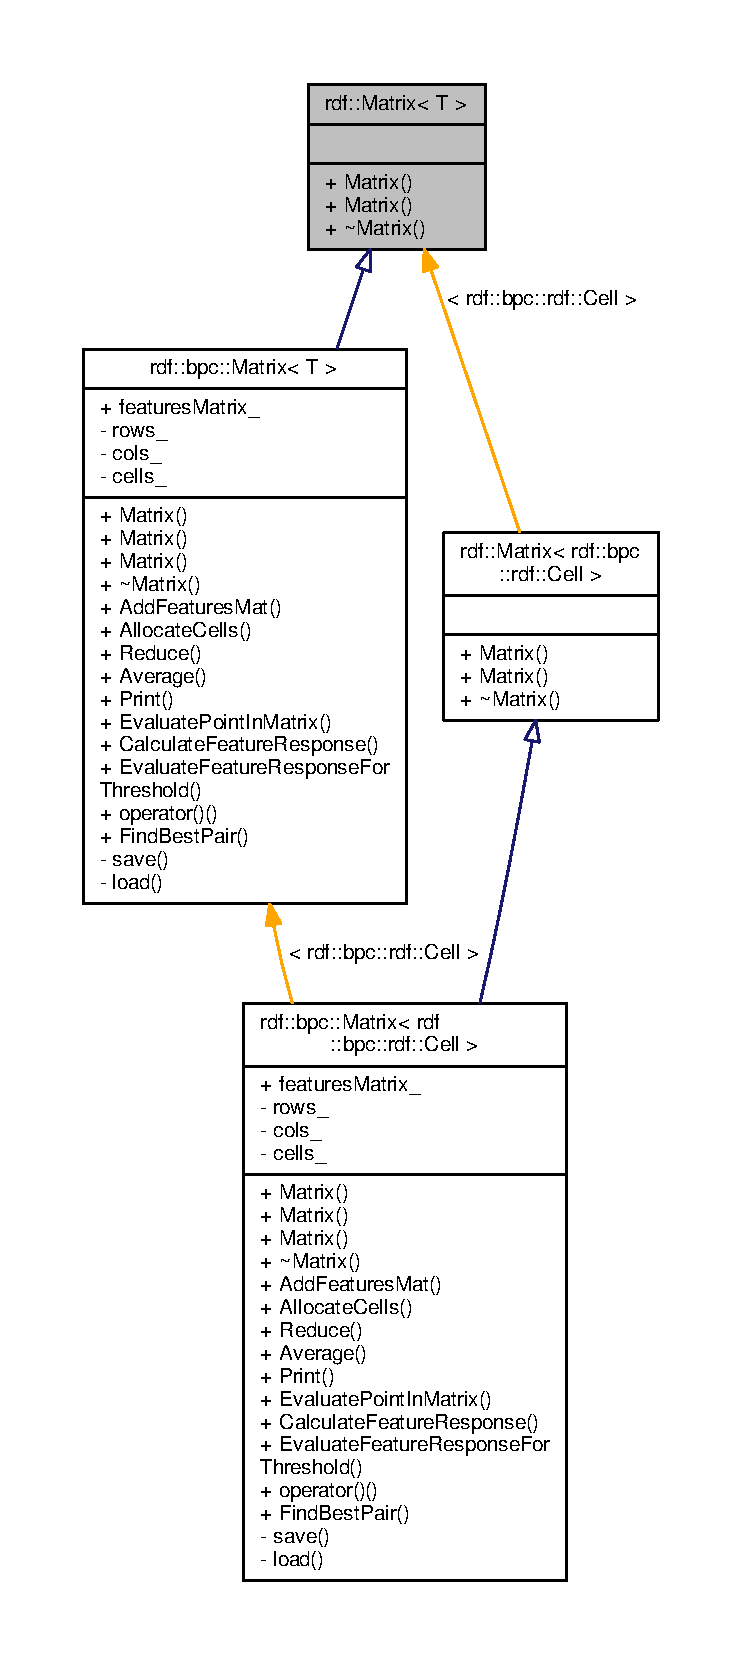
\includegraphics[height=550pt]{classrdf_1_1Matrix__inherit__graph}
\end{center}
\end{figure}


Collaboration diagram for rdf\+:\+:Matrix$<$ T $>$\+:
\nopagebreak
\begin{figure}[H]
\begin{center}
\leavevmode
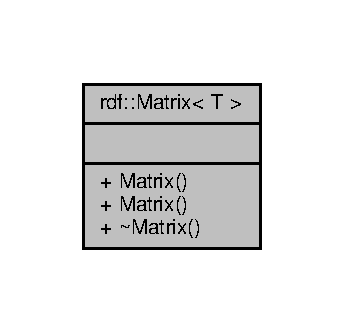
\includegraphics[width=165pt]{classrdf_1_1Matrix__coll__graph}
\end{center}
\end{figure}
\subsection*{Public Member Functions}
\begin{DoxyCompactItemize}
\item 
\hyperlink{classrdf_1_1Matrix_aa128192dbb2f8daf356bc76244104eab}{Matrix} ()
\item 
\hyperlink{classrdf_1_1Matrix_ae2c663aa421b4982c9edb0bf022b5b94}{Matrix} (const \hyperlink{classrdf_1_1Matrix}{Matrix} \&orig)
\item 
virtual \hyperlink{classrdf_1_1Matrix_a03f03cfa4c03e106714e2975ecafb892}{$\sim$\+Matrix} ()
\end{DoxyCompactItemize}


\subsection{Constructor \& Destructor Documentation}
\index{rdf\+::\+Matrix@{rdf\+::\+Matrix}!Matrix@{Matrix}}
\index{Matrix@{Matrix}!rdf\+::\+Matrix@{rdf\+::\+Matrix}}
\subsubsection[{\texorpdfstring{Matrix()}{Matrix()}}]{\setlength{\rightskip}{0pt plus 5cm}template$<$typename T$>$ {\bf rdf\+::\+Matrix}$<$ T $>$\+::{\bf Matrix} (
\begin{DoxyParamCaption}
{}
\end{DoxyParamCaption}
)}\hypertarget{classrdf_1_1Matrix_aa128192dbb2f8daf356bc76244104eab}{}\label{classrdf_1_1Matrix_aa128192dbb2f8daf356bc76244104eab}
\index{rdf\+::\+Matrix@{rdf\+::\+Matrix}!Matrix@{Matrix}}
\index{Matrix@{Matrix}!rdf\+::\+Matrix@{rdf\+::\+Matrix}}
\subsubsection[{\texorpdfstring{Matrix(const Matrix \&orig)}{Matrix(const Matrix &orig)}}]{\setlength{\rightskip}{0pt plus 5cm}template$<$typename T$>$ {\bf rdf\+::\+Matrix}$<$ T $>$\+::{\bf Matrix} (
\begin{DoxyParamCaption}
\item[{const {\bf Matrix}$<$ T $>$ \&}]{orig}
\end{DoxyParamCaption}
)}\hypertarget{classrdf_1_1Matrix_ae2c663aa421b4982c9edb0bf022b5b94}{}\label{classrdf_1_1Matrix_ae2c663aa421b4982c9edb0bf022b5b94}
\index{rdf\+::\+Matrix@{rdf\+::\+Matrix}!````~Matrix@{$\sim$\+Matrix}}
\index{````~Matrix@{$\sim$\+Matrix}!rdf\+::\+Matrix@{rdf\+::\+Matrix}}
\subsubsection[{\texorpdfstring{$\sim$\+Matrix()}{~Matrix()}}]{\setlength{\rightskip}{0pt plus 5cm}template$<$typename T$>$ virtual {\bf rdf\+::\+Matrix}$<$ T $>$\+::$\sim${\bf Matrix} (
\begin{DoxyParamCaption}
{}
\end{DoxyParamCaption}
)\hspace{0.3cm}{\ttfamily [virtual]}}\hypertarget{classrdf_1_1Matrix_a03f03cfa4c03e106714e2975ecafb892}{}\label{classrdf_1_1Matrix_a03f03cfa4c03e106714e2975ecafb892}


Reimplemented in \hyperlink{classrdf_1_1bpc_1_1Matrix_ab7cf40ce5404d7727a0a656e8c739140}{rdf\+::bpc\+::\+Matrix$<$ T $>$}, and \hyperlink{classrdf_1_1bpc_1_1Matrix_ab7cf40ce5404d7727a0a656e8c739140}{rdf\+::bpc\+::\+Matrix$<$ rdf\+::bpc\+::rdf\+::\+Cell $>$}.



The documentation for this class was generated from the following file\+:\begin{DoxyCompactItemize}
\item 
\hyperlink{Matrix_8h}{Matrix.\+h}\end{DoxyCompactItemize}

\hypertarget{classrdf_1_1bpc_1_1Matrix}{}\section{rdf\+:\+:bpc\+:\+:Matrix$<$ T $>$ Class Template Reference}
\label{classrdf_1_1bpc_1_1Matrix}\index{rdf\+::bpc\+::\+Matrix$<$ T $>$@{rdf\+::bpc\+::\+Matrix$<$ T $>$}}


{\ttfamily \#include $<$Features\+Mat.\+h$>$}



Inheritance diagram for rdf\+:\+:bpc\+:\+:Matrix$<$ T $>$\+:
\nopagebreak
\begin{figure}[H]
\begin{center}
\leavevmode
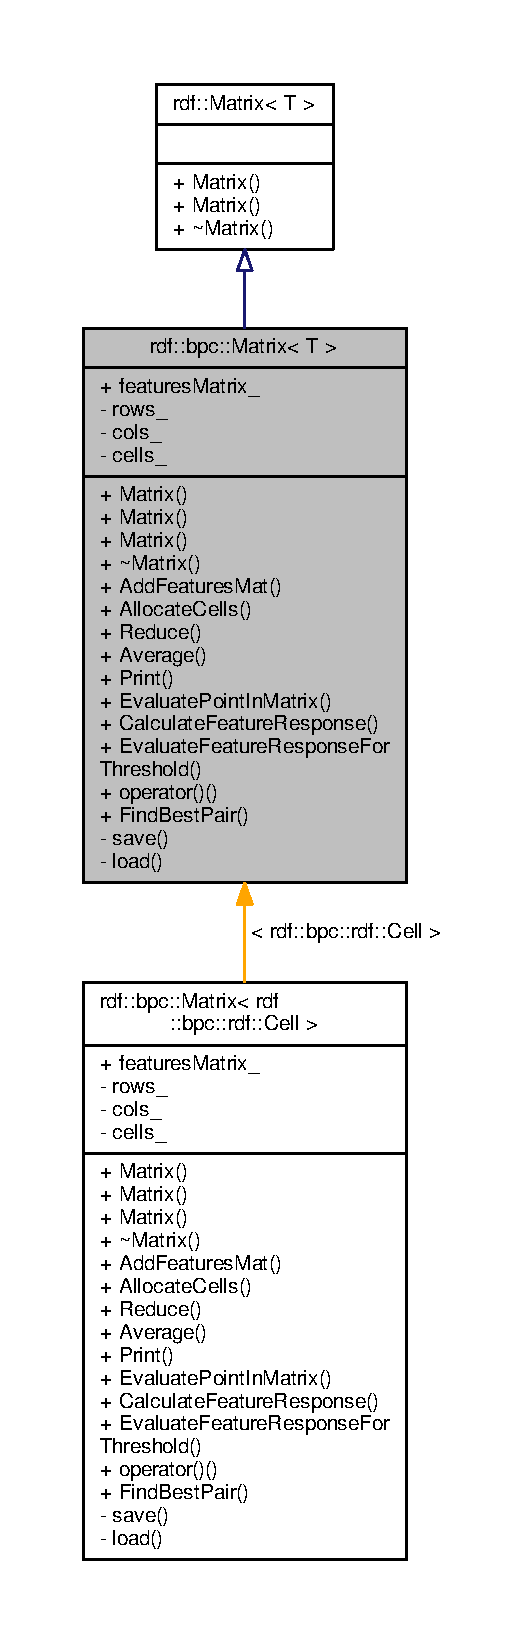
\includegraphics[height=550pt]{classrdf_1_1bpc_1_1Matrix__inherit__graph}
\end{center}
\end{figure}


Collaboration diagram for rdf\+:\+:bpc\+:\+:Matrix$<$ T $>$\+:
\nopagebreak
\begin{figure}[H]
\begin{center}
\leavevmode
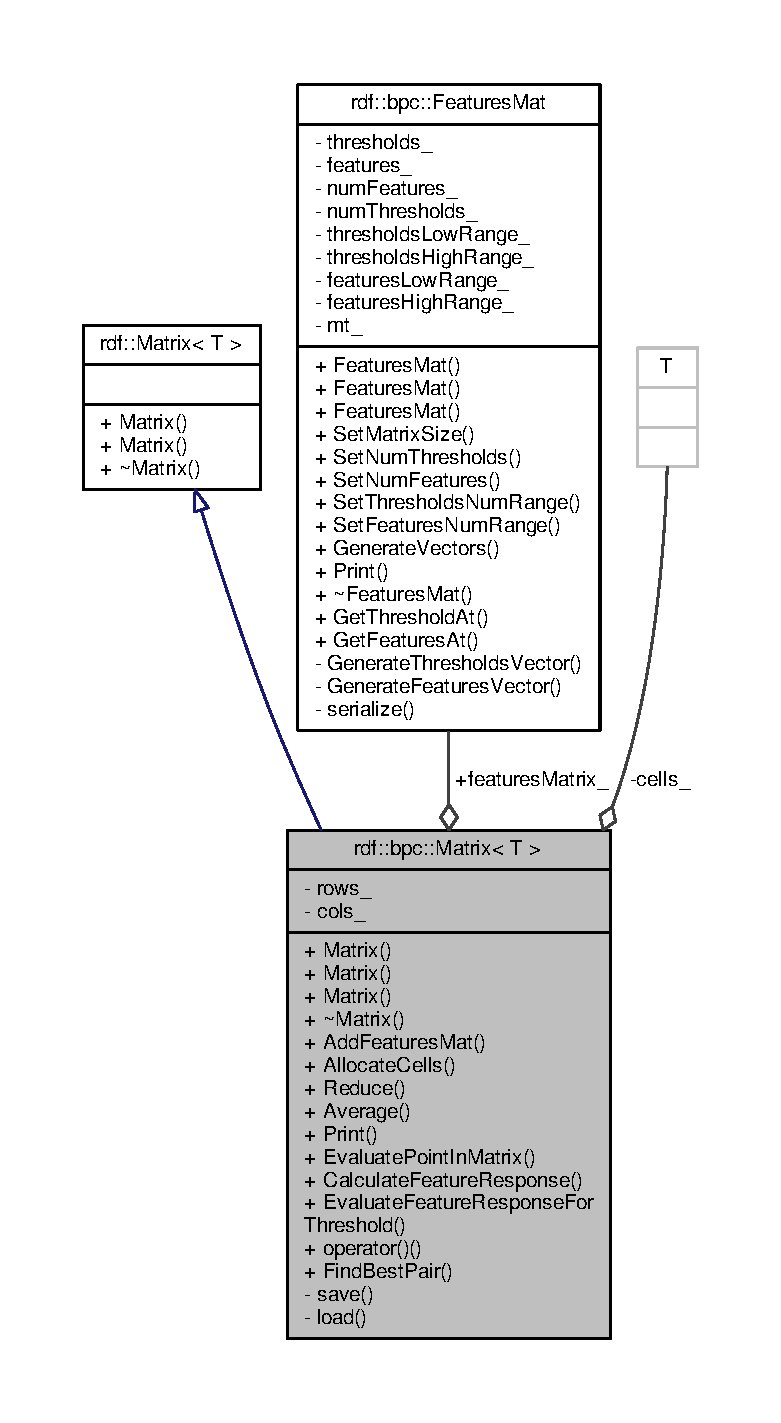
\includegraphics[height=550pt]{classrdf_1_1bpc_1_1Matrix__coll__graph}
\end{center}
\end{figure}
\subsection*{Public Member Functions}
\begin{DoxyCompactItemize}
\item 
\hyperlink{classrdf_1_1bpc_1_1Matrix_ade45ad0ebe3b9c850608a4f5abb19420}{Matrix} ()
\item 
\hyperlink{classrdf_1_1bpc_1_1Matrix_a2bc9d43380289047df29a49cbbda1067}{Matrix} (const \hyperlink{classrdf_1_1bpc_1_1FeaturesMat}{Features\+Mat} \&)
\item 
\hyperlink{classrdf_1_1bpc_1_1Matrix_a2ec31b288ce0fbdacf2310446f3ace38}{Matrix} (const \hyperlink{classrdf_1_1bpc_1_1Matrix}{Matrix} \&orig)
\item 
virtual \hyperlink{classrdf_1_1bpc_1_1Matrix_ab7cf40ce5404d7727a0a656e8c739140}{$\sim$\+Matrix} ()
\item 
void \hyperlink{classrdf_1_1bpc_1_1Matrix_a937666077b21230acd1afe126f84a7b4}{Add\+Features\+Mat} (const \hyperlink{classrdf_1_1bpc_1_1FeaturesMat}{Features\+Mat} \&mat)
\item 
void \hyperlink{classrdf_1_1bpc_1_1Matrix_ac90210cef7b4b102b3ec19d78a38631d}{Allocate\+Cells} ()
\item 
void \hyperlink{classrdf_1_1bpc_1_1Matrix_a45f64dbd9f56ee67d906aa08961bbae9}{Reduce} (\hyperlink{classrdf_1_1bpc_1_1Matrix}{Matrix} \&other)
\item 
void \hyperlink{classrdf_1_1bpc_1_1Matrix_a480cb47beacfcc5809503893fc38b968}{Average} (int average)
\item 
void \hyperlink{classrdf_1_1bpc_1_1Matrix_acb261eb27775f1ed974349f7ceb6c1c3}{Print} ()
\item 
void \hyperlink{classrdf_1_1bpc_1_1Matrix_a05799bd5cff0c7c1d1c4f6fa19dce22b}{Evaluate\+Point\+In\+Matrix} (int point)
\item 
float \hyperlink{classrdf_1_1bpc_1_1Matrix_a3884af4b2109a2d80b2dc2778bd71a8e}{Calculate\+Feature\+Response} (int, int, int)
\item 
bool \hyperlink{classrdf_1_1bpc_1_1Matrix_a81c5040bdc90a4548ebedc0e3027d666}{Evaluate\+Feature\+Response\+For\+Threshold} (float, int)
\item 
T \hyperlink{classrdf_1_1bpc_1_1Matrix_a950b7d0d97347c41047d8e5631552e58}{operator()} (int i, int j)
\item 
std\+::pair$<$ int, int $>$ \hyperlink{classrdf_1_1bpc_1_1Matrix_ab6cf5e854c06f976908b4f53462b6bd3}{Find\+Best\+Pair} ()
\end{DoxyCompactItemize}
\subsection*{Public Attributes}
\begin{DoxyCompactItemize}
\item 
\hyperlink{classrdf_1_1bpc_1_1FeaturesMat}{Features\+Mat} \hyperlink{classrdf_1_1bpc_1_1Matrix_a635849575c43df7969d5328cede7a040}{features\+Matrix\+\_\+}
\end{DoxyCompactItemize}
\subsection*{Private Member Functions}
\begin{DoxyCompactItemize}
\item 
{\footnotesize template$<$class Archive $>$ }\\void \hyperlink{classrdf_1_1bpc_1_1Matrix_a6c3808d393e218a29df6ff1bbdfbe8ea}{save} (Archive \&ar, const unsigned int version) const 
\item 
{\footnotesize template$<$class Archive $>$ }\\void \hyperlink{classrdf_1_1bpc_1_1Matrix_a87e3e793dc7e2fa499aaba37bf825510}{load} (Archive \&ar, const unsigned int version)
\end{DoxyCompactItemize}
\subsection*{Private Attributes}
\begin{DoxyCompactItemize}
\item 
int \hyperlink{classrdf_1_1bpc_1_1Matrix_a594473393d0fb508cf68714062f65256}{rows\+\_\+}
\item 
int \hyperlink{classrdf_1_1bpc_1_1Matrix_a2a15ca3ef49e2f0c7724e5c556878b3c}{cols\+\_\+}
\item 
T $\ast$ \hyperlink{classrdf_1_1bpc_1_1Matrix_adebf06eb7c44da98fd103edfb17988f1}{cells\+\_\+}
\end{DoxyCompactItemize}
\subsection*{Friends}
\begin{DoxyCompactItemize}
\item 
class \hyperlink{classrdf_1_1bpc_1_1Matrix_ac98d07dd8f7b70e16ccb9a01abf56b9c}{boost\+::serialization\+::access}
\end{DoxyCompactItemize}


\subsection{Constructor \& Destructor Documentation}
\index{rdf\+::bpc\+::\+Matrix@{rdf\+::bpc\+::\+Matrix}!Matrix@{Matrix}}
\index{Matrix@{Matrix}!rdf\+::bpc\+::\+Matrix@{rdf\+::bpc\+::\+Matrix}}
\subsubsection[{\texorpdfstring{Matrix()}{Matrix()}}]{\setlength{\rightskip}{0pt plus 5cm}template$<$typename T$>$ {\bf rdf\+::bpc\+::\+Matrix}$<$ T $>$\+::{\bf Matrix} (
\begin{DoxyParamCaption}
{}
\end{DoxyParamCaption}
)}\hypertarget{classrdf_1_1bpc_1_1Matrix_ade45ad0ebe3b9c850608a4f5abb19420}{}\label{classrdf_1_1bpc_1_1Matrix_ade45ad0ebe3b9c850608a4f5abb19420}
\index{rdf\+::bpc\+::\+Matrix@{rdf\+::bpc\+::\+Matrix}!Matrix@{Matrix}}
\index{Matrix@{Matrix}!rdf\+::bpc\+::\+Matrix@{rdf\+::bpc\+::\+Matrix}}
\subsubsection[{\texorpdfstring{Matrix(const Features\+Mat \&)}{Matrix(const FeaturesMat &)}}]{\setlength{\rightskip}{0pt plus 5cm}template$<$typename T$>$ {\bf rdf\+::bpc\+::\+Matrix}$<$ T $>$\+::{\bf Matrix} (
\begin{DoxyParamCaption}
\item[{const {\bf Features\+Mat} \&}]{}
\end{DoxyParamCaption}
)}\hypertarget{classrdf_1_1bpc_1_1Matrix_a2bc9d43380289047df29a49cbbda1067}{}\label{classrdf_1_1bpc_1_1Matrix_a2bc9d43380289047df29a49cbbda1067}
\index{rdf\+::bpc\+::\+Matrix@{rdf\+::bpc\+::\+Matrix}!Matrix@{Matrix}}
\index{Matrix@{Matrix}!rdf\+::bpc\+::\+Matrix@{rdf\+::bpc\+::\+Matrix}}
\subsubsection[{\texorpdfstring{Matrix(const Matrix \&orig)}{Matrix(const Matrix &orig)}}]{\setlength{\rightskip}{0pt plus 5cm}template$<$typename T$>$ {\bf rdf\+::bpc\+::\+Matrix}$<$ T $>$\+::{\bf Matrix} (
\begin{DoxyParamCaption}
\item[{const {\bf Matrix}$<$ T $>$ \&}]{orig}
\end{DoxyParamCaption}
)}\hypertarget{classrdf_1_1bpc_1_1Matrix_a2ec31b288ce0fbdacf2310446f3ace38}{}\label{classrdf_1_1bpc_1_1Matrix_a2ec31b288ce0fbdacf2310446f3ace38}
\index{rdf\+::bpc\+::\+Matrix@{rdf\+::bpc\+::\+Matrix}!````~Matrix@{$\sim$\+Matrix}}
\index{````~Matrix@{$\sim$\+Matrix}!rdf\+::bpc\+::\+Matrix@{rdf\+::bpc\+::\+Matrix}}
\subsubsection[{\texorpdfstring{$\sim$\+Matrix()}{~Matrix()}}]{\setlength{\rightskip}{0pt plus 5cm}template$<$typename T$>$ virtual {\bf rdf\+::bpc\+::\+Matrix}$<$ T $>$\+::$\sim${\bf Matrix} (
\begin{DoxyParamCaption}
{}
\end{DoxyParamCaption}
)\hspace{0.3cm}{\ttfamily [virtual]}}\hypertarget{classrdf_1_1bpc_1_1Matrix_ab7cf40ce5404d7727a0a656e8c739140}{}\label{classrdf_1_1bpc_1_1Matrix_ab7cf40ce5404d7727a0a656e8c739140}


Reimplemented from \hyperlink{classrdf_1_1Matrix_a03f03cfa4c03e106714e2975ecafb892}{rdf\+::\+Matrix$<$ T $>$}.



\subsection{Member Function Documentation}
\index{rdf\+::bpc\+::\+Matrix@{rdf\+::bpc\+::\+Matrix}!Add\+Features\+Mat@{Add\+Features\+Mat}}
\index{Add\+Features\+Mat@{Add\+Features\+Mat}!rdf\+::bpc\+::\+Matrix@{rdf\+::bpc\+::\+Matrix}}
\subsubsection[{\texorpdfstring{Add\+Features\+Mat(const Features\+Mat \&mat)}{AddFeaturesMat(const FeaturesMat &mat)}}]{\setlength{\rightskip}{0pt plus 5cm}template$<$typename T$>$ void {\bf rdf\+::bpc\+::\+Matrix}$<$ T $>$\+::Add\+Features\+Mat (
\begin{DoxyParamCaption}
\item[{const {\bf Features\+Mat} \&}]{mat}
\end{DoxyParamCaption}
)}\hypertarget{classrdf_1_1bpc_1_1Matrix_a937666077b21230acd1afe126f84a7b4}{}\label{classrdf_1_1bpc_1_1Matrix_a937666077b21230acd1afe126f84a7b4}
\index{rdf\+::bpc\+::\+Matrix@{rdf\+::bpc\+::\+Matrix}!Allocate\+Cells@{Allocate\+Cells}}
\index{Allocate\+Cells@{Allocate\+Cells}!rdf\+::bpc\+::\+Matrix@{rdf\+::bpc\+::\+Matrix}}
\subsubsection[{\texorpdfstring{Allocate\+Cells()}{AllocateCells()}}]{\setlength{\rightskip}{0pt plus 5cm}template$<$typename T$>$ void {\bf rdf\+::bpc\+::\+Matrix}$<$ T $>$\+::Allocate\+Cells (
\begin{DoxyParamCaption}
{}
\end{DoxyParamCaption}
)}\hypertarget{classrdf_1_1bpc_1_1Matrix_ac90210cef7b4b102b3ec19d78a38631d}{}\label{classrdf_1_1bpc_1_1Matrix_ac90210cef7b4b102b3ec19d78a38631d}


Referenced by rdf\+::bpc\+::\+Matrix$<$ rdf\+::bpc\+::rdf\+::\+Cell $>$\+::load().

\index{rdf\+::bpc\+::\+Matrix@{rdf\+::bpc\+::\+Matrix}!Average@{Average}}
\index{Average@{Average}!rdf\+::bpc\+::\+Matrix@{rdf\+::bpc\+::\+Matrix}}
\subsubsection[{\texorpdfstring{Average(int average)}{Average(int average)}}]{\setlength{\rightskip}{0pt plus 5cm}template$<$typename T$>$ void {\bf rdf\+::bpc\+::\+Matrix}$<$ T $>$\+::Average (
\begin{DoxyParamCaption}
\item[{int}]{average}
\end{DoxyParamCaption}
)}\hypertarget{classrdf_1_1bpc_1_1Matrix_a480cb47beacfcc5809503893fc38b968}{}\label{classrdf_1_1bpc_1_1Matrix_a480cb47beacfcc5809503893fc38b968}
\index{rdf\+::bpc\+::\+Matrix@{rdf\+::bpc\+::\+Matrix}!Calculate\+Feature\+Response@{Calculate\+Feature\+Response}}
\index{Calculate\+Feature\+Response@{Calculate\+Feature\+Response}!rdf\+::bpc\+::\+Matrix@{rdf\+::bpc\+::\+Matrix}}
\subsubsection[{\texorpdfstring{Calculate\+Feature\+Response(int, int, int)}{CalculateFeatureResponse(int, int, int)}}]{\setlength{\rightskip}{0pt plus 5cm}template$<$typename T$>$ float {\bf rdf\+::bpc\+::\+Matrix}$<$ T $>$\+::Calculate\+Feature\+Response (
\begin{DoxyParamCaption}
\item[{int}]{, }
\item[{int}]{, }
\item[{int}]{}
\end{DoxyParamCaption}
)}\hypertarget{classrdf_1_1bpc_1_1Matrix_a3884af4b2109a2d80b2dc2778bd71a8e}{}\label{classrdf_1_1bpc_1_1Matrix_a3884af4b2109a2d80b2dc2778bd71a8e}
\index{rdf\+::bpc\+::\+Matrix@{rdf\+::bpc\+::\+Matrix}!Evaluate\+Feature\+Response\+For\+Threshold@{Evaluate\+Feature\+Response\+For\+Threshold}}
\index{Evaluate\+Feature\+Response\+For\+Threshold@{Evaluate\+Feature\+Response\+For\+Threshold}!rdf\+::bpc\+::\+Matrix@{rdf\+::bpc\+::\+Matrix}}
\subsubsection[{\texorpdfstring{Evaluate\+Feature\+Response\+For\+Threshold(float, int)}{EvaluateFeatureResponseForThreshold(float, int)}}]{\setlength{\rightskip}{0pt plus 5cm}template$<$typename T$>$ bool {\bf rdf\+::bpc\+::\+Matrix}$<$ T $>$\+::Evaluate\+Feature\+Response\+For\+Threshold (
\begin{DoxyParamCaption}
\item[{float}]{, }
\item[{int}]{}
\end{DoxyParamCaption}
)}\hypertarget{classrdf_1_1bpc_1_1Matrix_a81c5040bdc90a4548ebedc0e3027d666}{}\label{classrdf_1_1bpc_1_1Matrix_a81c5040bdc90a4548ebedc0e3027d666}
\index{rdf\+::bpc\+::\+Matrix@{rdf\+::bpc\+::\+Matrix}!Evaluate\+Point\+In\+Matrix@{Evaluate\+Point\+In\+Matrix}}
\index{Evaluate\+Point\+In\+Matrix@{Evaluate\+Point\+In\+Matrix}!rdf\+::bpc\+::\+Matrix@{rdf\+::bpc\+::\+Matrix}}
\subsubsection[{\texorpdfstring{Evaluate\+Point\+In\+Matrix(int point)}{EvaluatePointInMatrix(int point)}}]{\setlength{\rightskip}{0pt plus 5cm}template$<$typename T$>$ void {\bf rdf\+::bpc\+::\+Matrix}$<$ T $>$\+::Evaluate\+Point\+In\+Matrix (
\begin{DoxyParamCaption}
\item[{int}]{point}
\end{DoxyParamCaption}
)}\hypertarget{classrdf_1_1bpc_1_1Matrix_a05799bd5cff0c7c1d1c4f6fa19dce22b}{}\label{classrdf_1_1bpc_1_1Matrix_a05799bd5cff0c7c1d1c4f6fa19dce22b}
\index{rdf\+::bpc\+::\+Matrix@{rdf\+::bpc\+::\+Matrix}!Find\+Best\+Pair@{Find\+Best\+Pair}}
\index{Find\+Best\+Pair@{Find\+Best\+Pair}!rdf\+::bpc\+::\+Matrix@{rdf\+::bpc\+::\+Matrix}}
\subsubsection[{\texorpdfstring{Find\+Best\+Pair()}{FindBestPair()}}]{\setlength{\rightskip}{0pt plus 5cm}template$<$typename T$>$ std\+::pair$<$int,int$>$ {\bf rdf\+::bpc\+::\+Matrix}$<$ T $>$\+::Find\+Best\+Pair (
\begin{DoxyParamCaption}
{}
\end{DoxyParamCaption}
)\hspace{0.3cm}{\ttfamily [inline]}}\hypertarget{classrdf_1_1bpc_1_1Matrix_ab6cf5e854c06f976908b4f53462b6bd3}{}\label{classrdf_1_1bpc_1_1Matrix_ab6cf5e854c06f976908b4f53462b6bd3}

\begin{DoxyCode}
61                                        \{
62            \textcolor{keywordflow}{return} std::make\_pair(2,3);
63          \}
\end{DoxyCode}
\index{rdf\+::bpc\+::\+Matrix@{rdf\+::bpc\+::\+Matrix}!load@{load}}
\index{load@{load}!rdf\+::bpc\+::\+Matrix@{rdf\+::bpc\+::\+Matrix}}
\subsubsection[{\texorpdfstring{load(\+Archive \&ar, const unsigned int version)}{load(Archive &ar, const unsigned int version)}}]{\setlength{\rightskip}{0pt plus 5cm}template$<$typename T$>$ template$<$class Archive $>$ void {\bf rdf\+::bpc\+::\+Matrix}$<$ T $>$\+::load (
\begin{DoxyParamCaption}
\item[{Archive \&}]{ar, }
\item[{const unsigned int}]{version}
\end{DoxyParamCaption}
)\hspace{0.3cm}{\ttfamily [inline]}, {\ttfamily [private]}}\hypertarget{classrdf_1_1bpc_1_1Matrix_a87e3e793dc7e2fa499aaba37bf825510}{}\label{classrdf_1_1bpc_1_1Matrix_a87e3e793dc7e2fa499aaba37bf825510}

\begin{DoxyCode}
90       \{
91         ar & \hyperlink{classrdf_1_1bpc_1_1Matrix_a635849575c43df7969d5328cede7a040}{featuresMatrix\_};
92         ar & \hyperlink{classrdf_1_1bpc_1_1Matrix_a594473393d0fb508cf68714062f65256}{rows\_};
93         ar & \hyperlink{classrdf_1_1bpc_1_1Matrix_a2a15ca3ef49e2f0c7724e5c556878b3c}{cols\_};
94         \hyperlink{classrdf_1_1bpc_1_1Matrix_ac90210cef7b4b102b3ec19d78a38631d}{AllocateCells}();
95         \textcolor{keywordflow}{for} (\textcolor{keywordtype}{size\_t} i = 0; i < \hyperlink{classrdf_1_1bpc_1_1Matrix_a594473393d0fb508cf68714062f65256}{rows\_}; i++) \{
96           \textcolor{keywordflow}{for} (\textcolor{keywordtype}{size\_t} j = 0; j < \hyperlink{classrdf_1_1bpc_1_1Matrix_a2a15ca3ef49e2f0c7724e5c556878b3c}{cols\_}; j++) \{
97             ar & \hyperlink{classrdf_1_1bpc_1_1Matrix_adebf06eb7c44da98fd103edfb17988f1}{cells\_}[i * rows\_ + j];
98           \}
99         \}
100       \}
\end{DoxyCode}
\index{rdf\+::bpc\+::\+Matrix@{rdf\+::bpc\+::\+Matrix}!operator()@{operator()}}
\index{operator()@{operator()}!rdf\+::bpc\+::\+Matrix@{rdf\+::bpc\+::\+Matrix}}
\subsubsection[{\texorpdfstring{operator()(int i, int j)}{operator()(int i, int j)}}]{\setlength{\rightskip}{0pt plus 5cm}template$<$typename T$>$ T {\bf rdf\+::bpc\+::\+Matrix}$<$ T $>$\+::operator() (
\begin{DoxyParamCaption}
\item[{int}]{i, }
\item[{int}]{j}
\end{DoxyParamCaption}
)\hspace{0.3cm}{\ttfamily [inline]}}\hypertarget{classrdf_1_1bpc_1_1Matrix_a950b7d0d97347c41047d8e5631552e58}{}\label{classrdf_1_1bpc_1_1Matrix_a950b7d0d97347c41047d8e5631552e58}

\begin{DoxyCode}
58                                     \{
59              \textcolor{keywordflow}{return} \hyperlink{classrdf_1_1bpc_1_1Matrix_adebf06eb7c44da98fd103edfb17988f1}{cells\_}[i * this->\hyperlink{classrdf_1_1bpc_1_1Matrix_a594473393d0fb508cf68714062f65256}{rows\_} + j];
60          \}
\end{DoxyCode}
\index{rdf\+::bpc\+::\+Matrix@{rdf\+::bpc\+::\+Matrix}!Print@{Print}}
\index{Print@{Print}!rdf\+::bpc\+::\+Matrix@{rdf\+::bpc\+::\+Matrix}}
\subsubsection[{\texorpdfstring{Print()}{Print()}}]{\setlength{\rightskip}{0pt plus 5cm}template$<$typename T$>$ void {\bf rdf\+::bpc\+::\+Matrix}$<$ T $>$\+::Print (
\begin{DoxyParamCaption}
{}
\end{DoxyParamCaption}
)}\hypertarget{classrdf_1_1bpc_1_1Matrix_acb261eb27775f1ed974349f7ceb6c1c3}{}\label{classrdf_1_1bpc_1_1Matrix_acb261eb27775f1ed974349f7ceb6c1c3}
\index{rdf\+::bpc\+::\+Matrix@{rdf\+::bpc\+::\+Matrix}!Reduce@{Reduce}}
\index{Reduce@{Reduce}!rdf\+::bpc\+::\+Matrix@{rdf\+::bpc\+::\+Matrix}}
\subsubsection[{\texorpdfstring{Reduce(\+Matrix \&other)}{Reduce(Matrix &other)}}]{\setlength{\rightskip}{0pt plus 5cm}template$<$typename T$>$ void {\bf rdf\+::bpc\+::\+Matrix}$<$ T $>$\+::Reduce (
\begin{DoxyParamCaption}
\item[{{\bf Matrix}$<$ T $>$ \&}]{other}
\end{DoxyParamCaption}
)}\hypertarget{classrdf_1_1bpc_1_1Matrix_a45f64dbd9f56ee67d906aa08961bbae9}{}\label{classrdf_1_1bpc_1_1Matrix_a45f64dbd9f56ee67d906aa08961bbae9}
\index{rdf\+::bpc\+::\+Matrix@{rdf\+::bpc\+::\+Matrix}!save@{save}}
\index{save@{save}!rdf\+::bpc\+::\+Matrix@{rdf\+::bpc\+::\+Matrix}}
\subsubsection[{\texorpdfstring{save(\+Archive \&ar, const unsigned int version) const }{save(Archive &ar, const unsigned int version) const }}]{\setlength{\rightskip}{0pt plus 5cm}template$<$typename T$>$ template$<$class Archive $>$ void {\bf rdf\+::bpc\+::\+Matrix}$<$ T $>$\+::save (
\begin{DoxyParamCaption}
\item[{Archive \&}]{ar, }
\item[{const unsigned int}]{version}
\end{DoxyParamCaption}
) const\hspace{0.3cm}{\ttfamily [inline]}, {\ttfamily [private]}}\hypertarget{classrdf_1_1bpc_1_1Matrix_a6c3808d393e218a29df6ff1bbdfbe8ea}{}\label{classrdf_1_1bpc_1_1Matrix_a6c3808d393e218a29df6ff1bbdfbe8ea}

\begin{DoxyCode}
78    \{
79      ar & \hyperlink{classrdf_1_1bpc_1_1Matrix_a635849575c43df7969d5328cede7a040}{featuresMatrix\_};
80      ar & \hyperlink{classrdf_1_1bpc_1_1Matrix_a594473393d0fb508cf68714062f65256}{rows\_};
81      ar & \hyperlink{classrdf_1_1bpc_1_1Matrix_a2a15ca3ef49e2f0c7724e5c556878b3c}{cols\_};
82      \textcolor{keywordflow}{for} (\textcolor{keywordtype}{size\_t} i = 0; i < \hyperlink{classrdf_1_1bpc_1_1Matrix_a594473393d0fb508cf68714062f65256}{rows\_}; i++) \{
83        \textcolor{keywordflow}{for} (\textcolor{keywordtype}{size\_t} j = 0; j < \hyperlink{classrdf_1_1bpc_1_1Matrix_a2a15ca3ef49e2f0c7724e5c556878b3c}{cols\_}; j++) \{
84          ar & \hyperlink{classrdf_1_1bpc_1_1Matrix_adebf06eb7c44da98fd103edfb17988f1}{cells\_}[i * rows\_ + j];
85        \}
86      \}
87    \}
\end{DoxyCode}


\subsection{Friends And Related Function Documentation}
\index{rdf\+::bpc\+::\+Matrix@{rdf\+::bpc\+::\+Matrix}!boost\+::serialization\+::access@{boost\+::serialization\+::access}}
\index{boost\+::serialization\+::access@{boost\+::serialization\+::access}!rdf\+::bpc\+::\+Matrix@{rdf\+::bpc\+::\+Matrix}}
\subsubsection[{\texorpdfstring{boost\+::serialization\+::access}{boost::serialization::access}}]{\setlength{\rightskip}{0pt plus 5cm}template$<$typename T$>$ friend class boost\+::serialization\+::access\hspace{0.3cm}{\ttfamily [friend]}}\hypertarget{classrdf_1_1bpc_1_1Matrix_ac98d07dd8f7b70e16ccb9a01abf56b9c}{}\label{classrdf_1_1bpc_1_1Matrix_ac98d07dd8f7b70e16ccb9a01abf56b9c}


\subsection{Member Data Documentation}
\index{rdf\+::bpc\+::\+Matrix@{rdf\+::bpc\+::\+Matrix}!cells\+\_\+@{cells\+\_\+}}
\index{cells\+\_\+@{cells\+\_\+}!rdf\+::bpc\+::\+Matrix@{rdf\+::bpc\+::\+Matrix}}
\subsubsection[{\texorpdfstring{cells\+\_\+}{cells_}}]{\setlength{\rightskip}{0pt plus 5cm}template$<$typename T$>$ T$\ast$ {\bf rdf\+::bpc\+::\+Matrix}$<$ T $>$\+::cells\+\_\+\hspace{0.3cm}{\ttfamily [private]}}\hypertarget{classrdf_1_1bpc_1_1Matrix_adebf06eb7c44da98fd103edfb17988f1}{}\label{classrdf_1_1bpc_1_1Matrix_adebf06eb7c44da98fd103edfb17988f1}


Referenced by rdf\+::bpc\+::\+Matrix$<$ rdf\+::bpc\+::rdf\+::\+Cell $>$\+::operator()().

\index{rdf\+::bpc\+::\+Matrix@{rdf\+::bpc\+::\+Matrix}!cols\+\_\+@{cols\+\_\+}}
\index{cols\+\_\+@{cols\+\_\+}!rdf\+::bpc\+::\+Matrix@{rdf\+::bpc\+::\+Matrix}}
\subsubsection[{\texorpdfstring{cols\+\_\+}{cols_}}]{\setlength{\rightskip}{0pt plus 5cm}template$<$typename T$>$ int {\bf rdf\+::bpc\+::\+Matrix}$<$ T $>$\+::cols\+\_\+\hspace{0.3cm}{\ttfamily [private]}}\hypertarget{classrdf_1_1bpc_1_1Matrix_a2a15ca3ef49e2f0c7724e5c556878b3c}{}\label{classrdf_1_1bpc_1_1Matrix_a2a15ca3ef49e2f0c7724e5c556878b3c}


Referenced by rdf\+::bpc\+::\+Matrix$<$ rdf\+::bpc\+::rdf\+::\+Cell $>$\+::load(), and rdf\+::bpc\+::\+Matrix$<$ rdf\+::bpc\+::rdf\+::\+Cell $>$\+::save().

\index{rdf\+::bpc\+::\+Matrix@{rdf\+::bpc\+::\+Matrix}!features\+Matrix\+\_\+@{features\+Matrix\+\_\+}}
\index{features\+Matrix\+\_\+@{features\+Matrix\+\_\+}!rdf\+::bpc\+::\+Matrix@{rdf\+::bpc\+::\+Matrix}}
\subsubsection[{\texorpdfstring{features\+Matrix\+\_\+}{featuresMatrix_}}]{\setlength{\rightskip}{0pt plus 5cm}template$<$typename T$>$ {\bf Features\+Mat} {\bf rdf\+::bpc\+::\+Matrix}$<$ T $>$\+::features\+Matrix\+\_\+}\hypertarget{classrdf_1_1bpc_1_1Matrix_a635849575c43df7969d5328cede7a040}{}\label{classrdf_1_1bpc_1_1Matrix_a635849575c43df7969d5328cede7a040}


Referenced by rdf\+::bpc\+::\+Matrix$<$ rdf\+::bpc\+::rdf\+::\+Cell $>$\+::load(), and rdf\+::bpc\+::\+Matrix$<$ rdf\+::bpc\+::rdf\+::\+Cell $>$\+::save().

\index{rdf\+::bpc\+::\+Matrix@{rdf\+::bpc\+::\+Matrix}!rows\+\_\+@{rows\+\_\+}}
\index{rows\+\_\+@{rows\+\_\+}!rdf\+::bpc\+::\+Matrix@{rdf\+::bpc\+::\+Matrix}}
\subsubsection[{\texorpdfstring{rows\+\_\+}{rows_}}]{\setlength{\rightskip}{0pt plus 5cm}template$<$typename T$>$ int {\bf rdf\+::bpc\+::\+Matrix}$<$ T $>$\+::rows\+\_\+\hspace{0.3cm}{\ttfamily [private]}}\hypertarget{classrdf_1_1bpc_1_1Matrix_a594473393d0fb508cf68714062f65256}{}\label{classrdf_1_1bpc_1_1Matrix_a594473393d0fb508cf68714062f65256}


Referenced by rdf\+::bpc\+::\+Matrix$<$ rdf\+::bpc\+::rdf\+::\+Cell $>$\+::load(), rdf\+::bpc\+::\+Matrix$<$ rdf\+::bpc\+::rdf\+::\+Cell $>$\+::operator()(), and rdf\+::bpc\+::\+Matrix$<$ rdf\+::bpc\+::rdf\+::\+Cell $>$\+::save().



The documentation for this class was generated from the following files\+:\begin{DoxyCompactItemize}
\item 
\hyperlink{FeaturesMat_8h}{Features\+Mat.\+h}\item 
\hyperlink{MatrixBPC_8h}{Matrix\+B\+P\+C.\+h}\end{DoxyCompactItemize}

\hypertarget{classMatrixBPCFeatures}{}\section{Matrix\+B\+P\+C\+Features$<$ T $>$ Class Template Reference}
\label{classMatrixBPCFeatures}\index{Matrix\+B\+P\+C\+Features$<$ T $>$@{Matrix\+B\+P\+C\+Features$<$ T $>$}}


{\ttfamily \#include $<$Matrix\+B\+P\+C\+Features.\+h$>$}



Collaboration diagram for Matrix\+B\+P\+C\+Features$<$ T $>$\+:
\nopagebreak
\begin{figure}[H]
\begin{center}
\leavevmode
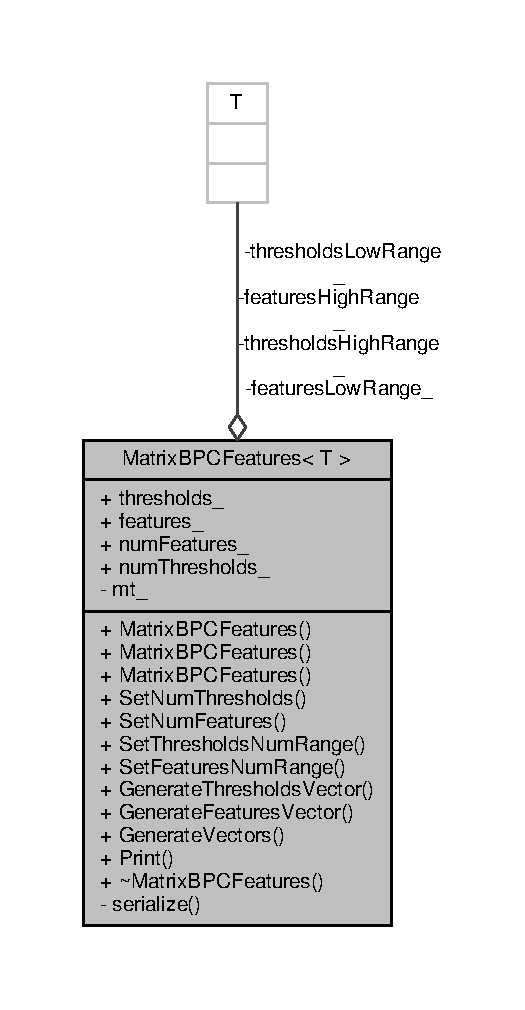
\includegraphics[width=252pt]{classMatrixBPCFeatures__coll__graph}
\end{center}
\end{figure}
\subsection*{Public Member Functions}
\begin{DoxyCompactItemize}
\item 
\hyperlink{classMatrixBPCFeatures_a72c1b182fac4397958ab20e37b58921e}{Matrix\+B\+P\+C\+Features} ()
\item 
\hyperlink{classMatrixBPCFeatures_afd6954e98b99e3ab09ad81082b9095d6}{Matrix\+B\+P\+C\+Features} (int fn, T fh, T fl, int tn, T th, T tl)
\item 
\hyperlink{classMatrixBPCFeatures_ad2bcf448da611be1417c6284b26b28ba}{Matrix\+B\+P\+C\+Features} (const \hyperlink{classMatrixBPCFeatures}{Matrix\+B\+P\+C\+Features} \&orig)
\item 
void \hyperlink{classMatrixBPCFeatures_ab26e57f5800162202aeaa38b719e9737}{Set\+Num\+Thresholds} (int)
\item 
void \hyperlink{classMatrixBPCFeatures_afd55350772c55d9608b8203734573b95}{Set\+Num\+Features} (int)
\item 
void \hyperlink{classMatrixBPCFeatures_a877df38950e5b68116e7ee8cdce764b2}{Set\+Thresholds\+Num\+Range} (T h, T l)
\item 
void \hyperlink{classMatrixBPCFeatures_a318a3a2a849eeb7e90b0be2454a61f61}{Set\+Features\+Num\+Range} (T h, T l)
\item 
void \hyperlink{classMatrixBPCFeatures_a912356bafe600e5625e21513d6f6ff71}{Generate\+Thresholds\+Vector} ()
\item 
void \hyperlink{classMatrixBPCFeatures_a25ae483a38966da88fd505f0536aa693}{Generate\+Features\+Vector} ()
\item 
void \hyperlink{classMatrixBPCFeatures_a710350735d6a54c8f936c9a3cb63db65}{Generate\+Vectors} ()
\item 
void \hyperlink{classMatrixBPCFeatures_a71ae3c997966a51917be4ca2f62f2e3e}{Print} ()
\item 
virtual \hyperlink{classMatrixBPCFeatures_a9d32e56c43b148b02ba325fd95479a1e}{$\sim$\+Matrix\+B\+P\+C\+Features} ()
\end{DoxyCompactItemize}
\subsection*{Public Attributes}
\begin{DoxyCompactItemize}
\item 
std\+::vector$<$ T $>$ \hyperlink{classMatrixBPCFeatures_a34418b525a7ceb5b2ec203415c46f066}{thresholds\+\_\+}
\item 
std\+::vector$<$ \hyperlink{MatrixBPCFeatures_8h_ab023c08b6db726ae7e0acc935755cfe6}{Features}$<$ T $>$ $>$ \hyperlink{classMatrixBPCFeatures_ad6ce34b650ac55b5d857a322cb239132}{features\+\_\+}
\item 
int \hyperlink{classMatrixBPCFeatures_ad3a5bf17a1666bbecf520f68d109b460}{num\+Features\+\_\+}
\item 
int \hyperlink{classMatrixBPCFeatures_adcdf00f112691ab61c3d305a3a9cbe89}{num\+Thresholds\+\_\+}
\end{DoxyCompactItemize}
\subsection*{Private Member Functions}
\begin{DoxyCompactItemize}
\item 
{\footnotesize template$<$class Archive $>$ }\\void \hyperlink{classMatrixBPCFeatures_ac1c62b0776f9a2f22f69b7debf86ecce}{serialize} (Archive \&ar, const unsigned int version)
\end{DoxyCompactItemize}
\subsection*{Private Attributes}
\begin{DoxyCompactItemize}
\item 
T \hyperlink{classMatrixBPCFeatures_a3b26efde265078abd546a45ea443bf6d}{thresholds\+Low\+Range\+\_\+}
\item 
T \hyperlink{classMatrixBPCFeatures_ae8a6cffe3353dfd370fb0b4e5d2385ca}{thresholds\+High\+Range\+\_\+}
\item 
T \hyperlink{classMatrixBPCFeatures_a973ec0283a77495339d330c482e73782}{features\+Low\+Range\+\_\+}
\item 
T \hyperlink{classMatrixBPCFeatures_a35acee240ac781db0390c068c782437d}{features\+High\+Range\+\_\+}
\end{DoxyCompactItemize}
\subsection*{Static Private Attributes}
\begin{DoxyCompactItemize}
\item 
static std\+::mt19937 \hyperlink{classMatrixBPCFeatures_aaf2ce60f69f7d3bbb85c4f4bc8b66383}{mt\+\_\+} = \hyperlink{MatrixBPCFeatures_8cpp_acd8f02610f7d92f49cfc5c5e0ad4c0da}{init2}()
\end{DoxyCompactItemize}
\subsection*{Friends}
\begin{DoxyCompactItemize}
\item 
class \hyperlink{classMatrixBPCFeatures_ac98d07dd8f7b70e16ccb9a01abf56b9c}{boost\+::serialization\+::access}
\end{DoxyCompactItemize}


\subsection{Constructor \& Destructor Documentation}
\index{Matrix\+B\+P\+C\+Features@{Matrix\+B\+P\+C\+Features}!Matrix\+B\+P\+C\+Features@{Matrix\+B\+P\+C\+Features}}
\index{Matrix\+B\+P\+C\+Features@{Matrix\+B\+P\+C\+Features}!Matrix\+B\+P\+C\+Features@{Matrix\+B\+P\+C\+Features}}
\subsubsection[{\texorpdfstring{Matrix\+B\+P\+C\+Features()}{MatrixBPCFeatures()}}]{\setlength{\rightskip}{0pt plus 5cm}template$<$typename T $>$ {\bf Matrix\+B\+P\+C\+Features}$<$ T $>$\+::{\bf Matrix\+B\+P\+C\+Features} (
\begin{DoxyParamCaption}
{}
\end{DoxyParamCaption}
)}\hypertarget{classMatrixBPCFeatures_a72c1b182fac4397958ab20e37b58921e}{}\label{classMatrixBPCFeatures_a72c1b182fac4397958ab20e37b58921e}

\begin{DoxyCode}
28                                         \{
29   \hyperlink{classMatrixBPCFeatures_ad3a5bf17a1666bbecf520f68d109b460}{numFeatures\_} = 0;
30   \hyperlink{classMatrixBPCFeatures_adcdf00f112691ab61c3d305a3a9cbe89}{numThresholds\_} = 0;
31   \hyperlink{classMatrixBPCFeatures_a35acee240ac781db0390c068c782437d}{featuresHighRange\_} = 0;
32   \hyperlink{classMatrixBPCFeatures_a973ec0283a77495339d330c482e73782}{featuresLowRange\_} = 0;
33   \hyperlink{classMatrixBPCFeatures_ae8a6cffe3353dfd370fb0b4e5d2385ca}{thresholdsHighRange\_} =  0;
34   \hyperlink{classMatrixBPCFeatures_a3b26efde265078abd546a45ea443bf6d}{thresholdsLowRange\_} = 0;
35 \}
\end{DoxyCode}
\index{Matrix\+B\+P\+C\+Features@{Matrix\+B\+P\+C\+Features}!Matrix\+B\+P\+C\+Features@{Matrix\+B\+P\+C\+Features}}
\index{Matrix\+B\+P\+C\+Features@{Matrix\+B\+P\+C\+Features}!Matrix\+B\+P\+C\+Features@{Matrix\+B\+P\+C\+Features}}
\subsubsection[{\texorpdfstring{Matrix\+B\+P\+C\+Features(int fn, T fh, T fl, int tn, T th, T tl)}{MatrixBPCFeatures(int fn, T fh, T fl, int tn, T th, T tl)}}]{\setlength{\rightskip}{0pt plus 5cm}template$<$typename T $>$ {\bf Matrix\+B\+P\+C\+Features}$<$ T $>$\+::{\bf Matrix\+B\+P\+C\+Features} (
\begin{DoxyParamCaption}
\item[{int}]{fn, }
\item[{T}]{fh, }
\item[{T}]{fl, }
\item[{int}]{tn, }
\item[{T}]{th, }
\item[{T}]{tl}
\end{DoxyParamCaption}
)}\hypertarget{classMatrixBPCFeatures_afd6954e98b99e3ab09ad81082b9095d6}{}\label{classMatrixBPCFeatures_afd6954e98b99e3ab09ad81082b9095d6}

\begin{DoxyCode}
39                                                                        \{
40     \hyperlink{classMatrixBPCFeatures_ad3a5bf17a1666bbecf520f68d109b460}{numFeatures\_} = numFeatures;
41     \hyperlink{classMatrixBPCFeatures_adcdf00f112691ab61c3d305a3a9cbe89}{numThresholds\_} = numThresholds;
42     \hyperlink{classMatrixBPCFeatures_a35acee240ac781db0390c068c782437d}{featuresHighRange\_} = featuresHigh;
43     \hyperlink{classMatrixBPCFeatures_a973ec0283a77495339d330c482e73782}{featuresLowRange\_} = featuresLow;
44     \hyperlink{classMatrixBPCFeatures_ae8a6cffe3353dfd370fb0b4e5d2385ca}{thresholdsHighRange\_} =  thresholdsHigh;
45     \hyperlink{classMatrixBPCFeatures_a3b26efde265078abd546a45ea443bf6d}{thresholdsLowRange\_} = thresholdsLow;
46 \}
\end{DoxyCode}
\index{Matrix\+B\+P\+C\+Features@{Matrix\+B\+P\+C\+Features}!Matrix\+B\+P\+C\+Features@{Matrix\+B\+P\+C\+Features}}
\index{Matrix\+B\+P\+C\+Features@{Matrix\+B\+P\+C\+Features}!Matrix\+B\+P\+C\+Features@{Matrix\+B\+P\+C\+Features}}
\subsubsection[{\texorpdfstring{Matrix\+B\+P\+C\+Features(const Matrix\+B\+P\+C\+Features \&orig)}{MatrixBPCFeatures(const MatrixBPCFeatures &orig)}}]{\setlength{\rightskip}{0pt plus 5cm}template$<$typename T $>$ {\bf Matrix\+B\+P\+C\+Features}$<$ T $>$\+::{\bf Matrix\+B\+P\+C\+Features} (
\begin{DoxyParamCaption}
\item[{const {\bf Matrix\+B\+P\+C\+Features}$<$ T $>$ \&}]{orig}
\end{DoxyParamCaption}
)}\hypertarget{classMatrixBPCFeatures_ad2bcf448da611be1417c6284b26b28ba}{}\label{classMatrixBPCFeatures_ad2bcf448da611be1417c6284b26b28ba}

\begin{DoxyCode}
50                                                                      \{
51 \}
\end{DoxyCode}
\index{Matrix\+B\+P\+C\+Features@{Matrix\+B\+P\+C\+Features}!````~Matrix\+B\+P\+C\+Features@{$\sim$\+Matrix\+B\+P\+C\+Features}}
\index{````~Matrix\+B\+P\+C\+Features@{$\sim$\+Matrix\+B\+P\+C\+Features}!Matrix\+B\+P\+C\+Features@{Matrix\+B\+P\+C\+Features}}
\subsubsection[{\texorpdfstring{$\sim$\+Matrix\+B\+P\+C\+Features()}{~MatrixBPCFeatures()}}]{\setlength{\rightskip}{0pt plus 5cm}template$<$typename T $>$ {\bf Matrix\+B\+P\+C\+Features}$<$ T $>$\+::$\sim${\bf Matrix\+B\+P\+C\+Features} (
\begin{DoxyParamCaption}
{}
\end{DoxyParamCaption}
)\hspace{0.3cm}{\ttfamily [virtual]}}\hypertarget{classMatrixBPCFeatures_a9d32e56c43b148b02ba325fd95479a1e}{}\label{classMatrixBPCFeatures_a9d32e56c43b148b02ba325fd95479a1e}

\begin{DoxyCode}
119                                          \{
120 \}
\end{DoxyCode}


\subsection{Member Function Documentation}
\index{Matrix\+B\+P\+C\+Features@{Matrix\+B\+P\+C\+Features}!Generate\+Features\+Vector@{Generate\+Features\+Vector}}
\index{Generate\+Features\+Vector@{Generate\+Features\+Vector}!Matrix\+B\+P\+C\+Features@{Matrix\+B\+P\+C\+Features}}
\subsubsection[{\texorpdfstring{Generate\+Features\+Vector()}{GenerateFeaturesVector()}}]{\setlength{\rightskip}{0pt plus 5cm}template$<$typename T $>$ void {\bf Matrix\+B\+P\+C\+Features}$<$ T $>$\+::Generate\+Features\+Vector (
\begin{DoxyParamCaption}
{}
\end{DoxyParamCaption}
)}\hypertarget{classMatrixBPCFeatures_a25ae483a38966da88fd505f0536aa693}{}\label{classMatrixBPCFeatures_a25ae483a38966da88fd505f0536aa693}

\begin{DoxyCode}
90                                                   \{
91     assert(\hyperlink{classMatrixBPCFeatures_ad3a5bf17a1666bbecf520f68d109b460}{numFeatures\_} > 0);
92     assert(\hyperlink{classMatrixBPCFeatures_a35acee240ac781db0390c068c782437d}{featuresHighRange\_} > \hyperlink{classMatrixBPCFeatures_a973ec0283a77495339d330c482e73782}{featuresLowRange\_});
93     std::uniform\_real\_distribution<T> features\_dist(\hyperlink{classMatrixBPCFeatures_a973ec0283a77495339d330c482e73782}{featuresLowRange\_}, 
      \hyperlink{classMatrixBPCFeatures_a35acee240ac781db0390c068c782437d}{featuresHighRange\_});
94     \textcolor{keywordflow}{for} (\textcolor{keywordtype}{size\_t} i = 0; i < \hyperlink{classMatrixBPCFeatures_ad3a5bf17a1666bbecf520f68d109b460}{numFeatures\_}; i++) \{
95         T randomFeature1 = features\_dist(\hyperlink{classMatrixBPCFeatures_aaf2ce60f69f7d3bbb85c4f4bc8b66383}{mt\_});
96         T randomFeature2 = features\_dist(\hyperlink{classMatrixBPCFeatures_aaf2ce60f69f7d3bbb85c4f4bc8b66383}{mt\_});
97         \hyperlink{MatrixBPCFeatures_8h_ab023c08b6db726ae7e0acc935755cfe6}{Features<T>} featuresPair = std::make\_pair(randomFeature1, randomFeature2);
98         \textcolor{comment}{// std::cout << "i-" << i << " F1: " << randomFeature1 << std::endl;}
99         \textcolor{comment}{// std::cout << "i-" << i << " F2: " << randomFeature2 << std::endl;}
100         \hyperlink{classMatrixBPCFeatures_ad6ce34b650ac55b5d857a322cb239132}{features\_}.push\_back(featuresPair);
101     \}
102 \}
\end{DoxyCode}
\index{Matrix\+B\+P\+C\+Features@{Matrix\+B\+P\+C\+Features}!Generate\+Thresholds\+Vector@{Generate\+Thresholds\+Vector}}
\index{Generate\+Thresholds\+Vector@{Generate\+Thresholds\+Vector}!Matrix\+B\+P\+C\+Features@{Matrix\+B\+P\+C\+Features}}
\subsubsection[{\texorpdfstring{Generate\+Thresholds\+Vector()}{GenerateThresholdsVector()}}]{\setlength{\rightskip}{0pt plus 5cm}template$<$typename T $>$ void {\bf Matrix\+B\+P\+C\+Features}$<$ T $>$\+::Generate\+Thresholds\+Vector (
\begin{DoxyParamCaption}
{}
\end{DoxyParamCaption}
)}\hypertarget{classMatrixBPCFeatures_a912356bafe600e5625e21513d6f6ff71}{}\label{classMatrixBPCFeatures_a912356bafe600e5625e21513d6f6ff71}

\begin{DoxyCode}
77                                                     \{
78   assert(\hyperlink{classMatrixBPCFeatures_adcdf00f112691ab61c3d305a3a9cbe89}{numThresholds\_} > 0);
79     assert(\hyperlink{classMatrixBPCFeatures_ae8a6cffe3353dfd370fb0b4e5d2385ca}{thresholdsHighRange\_} > \hyperlink{classMatrixBPCFeatures_a3b26efde265078abd546a45ea443bf6d}{thresholdsLowRange\_});
80     std::uniform\_real\_distribution<T> threshold\_dist(\hyperlink{classMatrixBPCFeatures_a3b26efde265078abd546a45ea443bf6d}{thresholdsLowRange\_}, 
      \hyperlink{classMatrixBPCFeatures_ae8a6cffe3353dfd370fb0b4e5d2385ca}{thresholdsHighRange\_});
81     \textcolor{keywordflow}{for} (\textcolor{keywordtype}{size\_t} i = 0; i < \hyperlink{classMatrixBPCFeatures_adcdf00f112691ab61c3d305a3a9cbe89}{numThresholds\_}; i++) \{
82         T randomThreshold = threshold\_dist(\hyperlink{classMatrixBPCFeatures_aaf2ce60f69f7d3bbb85c4f4bc8b66383}{mt\_});
83         \hyperlink{classMatrixBPCFeatures_a34418b525a7ceb5b2ec203415c46f066}{thresholds\_}.push\_back(randomThreshold);
84         \textcolor{comment}{// std::cout << "i-" << i << " T: " << thresholds\_[i] << std::endl;}
85     \}
86 \}
\end{DoxyCode}
\index{Matrix\+B\+P\+C\+Features@{Matrix\+B\+P\+C\+Features}!Generate\+Vectors@{Generate\+Vectors}}
\index{Generate\+Vectors@{Generate\+Vectors}!Matrix\+B\+P\+C\+Features@{Matrix\+B\+P\+C\+Features}}
\subsubsection[{\texorpdfstring{Generate\+Vectors()}{GenerateVectors()}}]{\setlength{\rightskip}{0pt plus 5cm}template$<$typename T $>$ void {\bf Matrix\+B\+P\+C\+Features}$<$ T $>$\+::Generate\+Vectors (
\begin{DoxyParamCaption}
{}
\end{DoxyParamCaption}
)}\hypertarget{classMatrixBPCFeatures_a710350735d6a54c8f936c9a3cb63db65}{}\label{classMatrixBPCFeatures_a710350735d6a54c8f936c9a3cb63db65}

\begin{DoxyCode}
105                                           \{
106   \hyperlink{classMatrixBPCFeatures_a912356bafe600e5625e21513d6f6ff71}{GenerateThresholdsVector}();
107   \hyperlink{classMatrixBPCFeatures_a25ae483a38966da88fd505f0536aa693}{GenerateFeaturesVector}();
108 \}
\end{DoxyCode}
\index{Matrix\+B\+P\+C\+Features@{Matrix\+B\+P\+C\+Features}!Print@{Print}}
\index{Print@{Print}!Matrix\+B\+P\+C\+Features@{Matrix\+B\+P\+C\+Features}}
\subsubsection[{\texorpdfstring{Print()}{Print()}}]{\setlength{\rightskip}{0pt plus 5cm}template$<$typename T $>$ void {\bf Matrix\+B\+P\+C\+Features}$<$ T $>$\+::Print (
\begin{DoxyParamCaption}
{}
\end{DoxyParamCaption}
)}\hypertarget{classMatrixBPCFeatures_a71ae3c997966a51917be4ca2f62f2e3e}{}\label{classMatrixBPCFeatures_a71ae3c997966a51917be4ca2f62f2e3e}

\begin{DoxyCode}
111                                 \{
112   \textcolor{keywordflow}{for} (\textcolor{keywordtype}{int} i = 0;  i < \hyperlink{classMatrixBPCFeatures_a34418b525a7ceb5b2ec203415c46f066}{thresholds\_}.size() ; i++) \{
113     \textcolor{comment}{// std::cerr << "Printing T[" << i << "]: " << thresholds\_.at(i) << std::endl;}
114   \}
115 \}
\end{DoxyCode}
\index{Matrix\+B\+P\+C\+Features@{Matrix\+B\+P\+C\+Features}!serialize@{serialize}}
\index{serialize@{serialize}!Matrix\+B\+P\+C\+Features@{Matrix\+B\+P\+C\+Features}}
\subsubsection[{\texorpdfstring{serialize(\+Archive \&ar, const unsigned int version)}{serialize(Archive &ar, const unsigned int version)}}]{\setlength{\rightskip}{0pt plus 5cm}template$<$typename T $>$ template$<$class Archive $>$ void {\bf Matrix\+B\+P\+C\+Features}$<$ T $>$\+::serialize (
\begin{DoxyParamCaption}
\item[{Archive \&}]{ar, }
\item[{const unsigned int}]{version}
\end{DoxyParamCaption}
)\hspace{0.3cm}{\ttfamily [inline]}, {\ttfamily [private]}}\hypertarget{classMatrixBPCFeatures_ac1c62b0776f9a2f22f69b7debf86ecce}{}\label{classMatrixBPCFeatures_ac1c62b0776f9a2f22f69b7debf86ecce}


References Matrix\+B\+P\+C\+Features$<$ T $>$\+::features\+\_\+, Matrix\+B\+P\+C\+Features$<$ T $>$\+::features\+High\+Range\+\_\+, Matrix\+B\+P\+C\+Features$<$ T $>$\+::features\+Low\+Range\+\_\+, Matrix\+B\+P\+C\+Features$<$ T $>$\+::num\+Features\+\_\+, Matrix\+B\+P\+C\+Features$<$ T $>$\+::num\+Thresholds\+\_\+, Matrix\+B\+P\+C\+Features$<$ T $>$\+::thresholds\+\_\+, Matrix\+B\+P\+C\+Features$<$ T $>$\+::thresholds\+High\+Range\+\_\+, and Matrix\+B\+P\+C\+Features$<$ T $>$\+::thresholds\+Low\+Range\+\_\+.


\begin{DoxyCode}
73     \{
74         ar & \hyperlink{classMatrixBPCFeatures_a34418b525a7ceb5b2ec203415c46f066}{thresholds\_};
75         ar & \hyperlink{classMatrixBPCFeatures_ad6ce34b650ac55b5d857a322cb239132}{features\_};
76         ar & \hyperlink{classMatrixBPCFeatures_ad3a5bf17a1666bbecf520f68d109b460}{numFeatures\_};
77         ar & \hyperlink{classMatrixBPCFeatures_adcdf00f112691ab61c3d305a3a9cbe89}{numThresholds\_};
78         ar & \hyperlink{classMatrixBPCFeatures_a3b26efde265078abd546a45ea443bf6d}{thresholdsLowRange\_};
79         ar & \hyperlink{classMatrixBPCFeatures_ae8a6cffe3353dfd370fb0b4e5d2385ca}{thresholdsHighRange\_};
80         ar & \hyperlink{classMatrixBPCFeatures_a973ec0283a77495339d330c482e73782}{featuresLowRange\_};
81         ar & \hyperlink{classMatrixBPCFeatures_a35acee240ac781db0390c068c782437d}{featuresHighRange\_};
82     \}
\end{DoxyCode}
\index{Matrix\+B\+P\+C\+Features@{Matrix\+B\+P\+C\+Features}!Set\+Features\+Num\+Range@{Set\+Features\+Num\+Range}}
\index{Set\+Features\+Num\+Range@{Set\+Features\+Num\+Range}!Matrix\+B\+P\+C\+Features@{Matrix\+B\+P\+C\+Features}}
\subsubsection[{\texorpdfstring{Set\+Features\+Num\+Range(\+T h, T l)}{SetFeaturesNumRange(T h, T l)}}]{\setlength{\rightskip}{0pt plus 5cm}template$<$typename T $>$ void {\bf Matrix\+B\+P\+C\+Features}$<$ T $>$\+::Set\+Features\+Num\+Range (
\begin{DoxyParamCaption}
\item[{T}]{h, }
\item[{T}]{l}
\end{DoxyParamCaption}
)}\hypertarget{classMatrixBPCFeatures_a318a3a2a849eeb7e90b0be2454a61f61}{}\label{classMatrixBPCFeatures_a318a3a2a849eeb7e90b0be2454a61f61}

\begin{DoxyCode}
71                                                             \{
72   \hyperlink{classMatrixBPCFeatures_a35acee240ac781db0390c068c782437d}{featuresHighRange\_} = high;
73     \hyperlink{classMatrixBPCFeatures_a973ec0283a77495339d330c482e73782}{featuresLowRange\_} = low;
74 \}
\end{DoxyCode}
\index{Matrix\+B\+P\+C\+Features@{Matrix\+B\+P\+C\+Features}!Set\+Num\+Features@{Set\+Num\+Features}}
\index{Set\+Num\+Features@{Set\+Num\+Features}!Matrix\+B\+P\+C\+Features@{Matrix\+B\+P\+C\+Features}}
\subsubsection[{\texorpdfstring{Set\+Num\+Features(int)}{SetNumFeatures(int)}}]{\setlength{\rightskip}{0pt plus 5cm}template$<$typename T $>$ void {\bf Matrix\+B\+P\+C\+Features}$<$ T $>$\+::Set\+Num\+Features (
\begin{DoxyParamCaption}
\item[{int}]{num\+Features}
\end{DoxyParamCaption}
)}\hypertarget{classMatrixBPCFeatures_afd55350772c55d9608b8203734573b95}{}\label{classMatrixBPCFeatures_afd55350772c55d9608b8203734573b95}

\begin{DoxyCode}
59                                                         \{
60   \hyperlink{classMatrixBPCFeatures_ad3a5bf17a1666bbecf520f68d109b460}{numFeatures\_} = numFeatures;
61 \}
\end{DoxyCode}
\index{Matrix\+B\+P\+C\+Features@{Matrix\+B\+P\+C\+Features}!Set\+Num\+Thresholds@{Set\+Num\+Thresholds}}
\index{Set\+Num\+Thresholds@{Set\+Num\+Thresholds}!Matrix\+B\+P\+C\+Features@{Matrix\+B\+P\+C\+Features}}
\subsubsection[{\texorpdfstring{Set\+Num\+Thresholds(int)}{SetNumThresholds(int)}}]{\setlength{\rightskip}{0pt plus 5cm}template$<$typename T $>$ void {\bf Matrix\+B\+P\+C\+Features}$<$ T $>$\+::Set\+Num\+Thresholds (
\begin{DoxyParamCaption}
\item[{int}]{num\+Thresholds}
\end{DoxyParamCaption}
)}\hypertarget{classMatrixBPCFeatures_ab26e57f5800162202aeaa38b719e9737}{}\label{classMatrixBPCFeatures_ab26e57f5800162202aeaa38b719e9737}

\begin{DoxyCode}
54                                                             \{
55   \hyperlink{classMatrixBPCFeatures_adcdf00f112691ab61c3d305a3a9cbe89}{numThresholds\_} = numThresholds;
56 \}
\end{DoxyCode}
\index{Matrix\+B\+P\+C\+Features@{Matrix\+B\+P\+C\+Features}!Set\+Thresholds\+Num\+Range@{Set\+Thresholds\+Num\+Range}}
\index{Set\+Thresholds\+Num\+Range@{Set\+Thresholds\+Num\+Range}!Matrix\+B\+P\+C\+Features@{Matrix\+B\+P\+C\+Features}}
\subsubsection[{\texorpdfstring{Set\+Thresholds\+Num\+Range(\+T h, T l)}{SetThresholdsNumRange(T h, T l)}}]{\setlength{\rightskip}{0pt plus 5cm}template$<$typename T $>$ void {\bf Matrix\+B\+P\+C\+Features}$<$ T $>$\+::Set\+Thresholds\+Num\+Range (
\begin{DoxyParamCaption}
\item[{T}]{h, }
\item[{T}]{l}
\end{DoxyParamCaption}
)}\hypertarget{classMatrixBPCFeatures_a877df38950e5b68116e7ee8cdce764b2}{}\label{classMatrixBPCFeatures_a877df38950e5b68116e7ee8cdce764b2}

\begin{DoxyCode}
64                                                              \{
65   \hyperlink{classMatrixBPCFeatures_ae8a6cffe3353dfd370fb0b4e5d2385ca}{thresholdsHighRange\_} = high;
66   \hyperlink{classMatrixBPCFeatures_a3b26efde265078abd546a45ea443bf6d}{thresholdsLowRange\_} = low;
67 \}
\end{DoxyCode}


\subsection{Friends And Related Function Documentation}
\index{Matrix\+B\+P\+C\+Features@{Matrix\+B\+P\+C\+Features}!boost\+::serialization\+::access@{boost\+::serialization\+::access}}
\index{boost\+::serialization\+::access@{boost\+::serialization\+::access}!Matrix\+B\+P\+C\+Features@{Matrix\+B\+P\+C\+Features}}
\subsubsection[{\texorpdfstring{boost\+::serialization\+::access}{boost::serialization::access}}]{\setlength{\rightskip}{0pt plus 5cm}template$<$typename T $>$ friend class boost\+::serialization\+::access\hspace{0.3cm}{\ttfamily [friend]}}\hypertarget{classMatrixBPCFeatures_ac98d07dd8f7b70e16ccb9a01abf56b9c}{}\label{classMatrixBPCFeatures_ac98d07dd8f7b70e16ccb9a01abf56b9c}


\subsection{Member Data Documentation}
\index{Matrix\+B\+P\+C\+Features@{Matrix\+B\+P\+C\+Features}!features\+\_\+@{features\+\_\+}}
\index{features\+\_\+@{features\+\_\+}!Matrix\+B\+P\+C\+Features@{Matrix\+B\+P\+C\+Features}}
\subsubsection[{\texorpdfstring{features\+\_\+}{features_}}]{\setlength{\rightskip}{0pt plus 5cm}template$<$typename T $>$ std\+::vector$<${\bf Features}$<$T$>$ $>$ {\bf Matrix\+B\+P\+C\+Features}$<$ T $>$\+::features\+\_\+}\hypertarget{classMatrixBPCFeatures_ad6ce34b650ac55b5d857a322cb239132}{}\label{classMatrixBPCFeatures_ad6ce34b650ac55b5d857a322cb239132}


Referenced by Matrix\+B\+P\+C\+Features$<$ T $>$\+::serialize().

\index{Matrix\+B\+P\+C\+Features@{Matrix\+B\+P\+C\+Features}!features\+High\+Range\+\_\+@{features\+High\+Range\+\_\+}}
\index{features\+High\+Range\+\_\+@{features\+High\+Range\+\_\+}!Matrix\+B\+P\+C\+Features@{Matrix\+B\+P\+C\+Features}}
\subsubsection[{\texorpdfstring{features\+High\+Range\+\_\+}{featuresHighRange_}}]{\setlength{\rightskip}{0pt plus 5cm}template$<$typename T $>$ T {\bf Matrix\+B\+P\+C\+Features}$<$ T $>$\+::features\+High\+Range\+\_\+\hspace{0.3cm}{\ttfamily [private]}}\hypertarget{classMatrixBPCFeatures_a35acee240ac781db0390c068c782437d}{}\label{classMatrixBPCFeatures_a35acee240ac781db0390c068c782437d}


Referenced by Matrix\+B\+P\+C\+Features$<$ T $>$\+::serialize().

\index{Matrix\+B\+P\+C\+Features@{Matrix\+B\+P\+C\+Features}!features\+Low\+Range\+\_\+@{features\+Low\+Range\+\_\+}}
\index{features\+Low\+Range\+\_\+@{features\+Low\+Range\+\_\+}!Matrix\+B\+P\+C\+Features@{Matrix\+B\+P\+C\+Features}}
\subsubsection[{\texorpdfstring{features\+Low\+Range\+\_\+}{featuresLowRange_}}]{\setlength{\rightskip}{0pt plus 5cm}template$<$typename T $>$ T {\bf Matrix\+B\+P\+C\+Features}$<$ T $>$\+::features\+Low\+Range\+\_\+\hspace{0.3cm}{\ttfamily [private]}}\hypertarget{classMatrixBPCFeatures_a973ec0283a77495339d330c482e73782}{}\label{classMatrixBPCFeatures_a973ec0283a77495339d330c482e73782}


Referenced by Matrix\+B\+P\+C\+Features$<$ T $>$\+::serialize().

\index{Matrix\+B\+P\+C\+Features@{Matrix\+B\+P\+C\+Features}!mt\+\_\+@{mt\+\_\+}}
\index{mt\+\_\+@{mt\+\_\+}!Matrix\+B\+P\+C\+Features@{Matrix\+B\+P\+C\+Features}}
\subsubsection[{\texorpdfstring{mt\+\_\+}{mt_}}]{\setlength{\rightskip}{0pt plus 5cm}template$<$typename T $>$ std\+::mt19937 {\bf Matrix\+B\+P\+C\+Features}$<$ T $>$\+::mt\+\_\+ = {\bf init2}()\hspace{0.3cm}{\ttfamily [static]}, {\ttfamily [private]}}\hypertarget{classMatrixBPCFeatures_aaf2ce60f69f7d3bbb85c4f4bc8b66383}{}\label{classMatrixBPCFeatures_aaf2ce60f69f7d3bbb85c4f4bc8b66383}
\index{Matrix\+B\+P\+C\+Features@{Matrix\+B\+P\+C\+Features}!num\+Features\+\_\+@{num\+Features\+\_\+}}
\index{num\+Features\+\_\+@{num\+Features\+\_\+}!Matrix\+B\+P\+C\+Features@{Matrix\+B\+P\+C\+Features}}
\subsubsection[{\texorpdfstring{num\+Features\+\_\+}{numFeatures_}}]{\setlength{\rightskip}{0pt plus 5cm}template$<$typename T $>$ int {\bf Matrix\+B\+P\+C\+Features}$<$ T $>$\+::num\+Features\+\_\+}\hypertarget{classMatrixBPCFeatures_ad3a5bf17a1666bbecf520f68d109b460}{}\label{classMatrixBPCFeatures_ad3a5bf17a1666bbecf520f68d109b460}


Referenced by Matrix\+B\+P\+C\+Features$<$ T $>$\+::serialize().

\index{Matrix\+B\+P\+C\+Features@{Matrix\+B\+P\+C\+Features}!num\+Thresholds\+\_\+@{num\+Thresholds\+\_\+}}
\index{num\+Thresholds\+\_\+@{num\+Thresholds\+\_\+}!Matrix\+B\+P\+C\+Features@{Matrix\+B\+P\+C\+Features}}
\subsubsection[{\texorpdfstring{num\+Thresholds\+\_\+}{numThresholds_}}]{\setlength{\rightskip}{0pt plus 5cm}template$<$typename T $>$ int {\bf Matrix\+B\+P\+C\+Features}$<$ T $>$\+::num\+Thresholds\+\_\+}\hypertarget{classMatrixBPCFeatures_adcdf00f112691ab61c3d305a3a9cbe89}{}\label{classMatrixBPCFeatures_adcdf00f112691ab61c3d305a3a9cbe89}


Referenced by Matrix\+B\+P\+C\+Features$<$ T $>$\+::serialize().

\index{Matrix\+B\+P\+C\+Features@{Matrix\+B\+P\+C\+Features}!thresholds\+\_\+@{thresholds\+\_\+}}
\index{thresholds\+\_\+@{thresholds\+\_\+}!Matrix\+B\+P\+C\+Features@{Matrix\+B\+P\+C\+Features}}
\subsubsection[{\texorpdfstring{thresholds\+\_\+}{thresholds_}}]{\setlength{\rightskip}{0pt plus 5cm}template$<$typename T $>$ std\+::vector$<$T$>$ {\bf Matrix\+B\+P\+C\+Features}$<$ T $>$\+::thresholds\+\_\+}\hypertarget{classMatrixBPCFeatures_a34418b525a7ceb5b2ec203415c46f066}{}\label{classMatrixBPCFeatures_a34418b525a7ceb5b2ec203415c46f066}


Referenced by Matrix\+B\+P\+C\+Features$<$ T $>$\+::serialize().

\index{Matrix\+B\+P\+C\+Features@{Matrix\+B\+P\+C\+Features}!thresholds\+High\+Range\+\_\+@{thresholds\+High\+Range\+\_\+}}
\index{thresholds\+High\+Range\+\_\+@{thresholds\+High\+Range\+\_\+}!Matrix\+B\+P\+C\+Features@{Matrix\+B\+P\+C\+Features}}
\subsubsection[{\texorpdfstring{thresholds\+High\+Range\+\_\+}{thresholdsHighRange_}}]{\setlength{\rightskip}{0pt plus 5cm}template$<$typename T $>$ T {\bf Matrix\+B\+P\+C\+Features}$<$ T $>$\+::thresholds\+High\+Range\+\_\+\hspace{0.3cm}{\ttfamily [private]}}\hypertarget{classMatrixBPCFeatures_ae8a6cffe3353dfd370fb0b4e5d2385ca}{}\label{classMatrixBPCFeatures_ae8a6cffe3353dfd370fb0b4e5d2385ca}


Referenced by Matrix\+B\+P\+C\+Features$<$ T $>$\+::serialize().

\index{Matrix\+B\+P\+C\+Features@{Matrix\+B\+P\+C\+Features}!thresholds\+Low\+Range\+\_\+@{thresholds\+Low\+Range\+\_\+}}
\index{thresholds\+Low\+Range\+\_\+@{thresholds\+Low\+Range\+\_\+}!Matrix\+B\+P\+C\+Features@{Matrix\+B\+P\+C\+Features}}
\subsubsection[{\texorpdfstring{thresholds\+Low\+Range\+\_\+}{thresholdsLowRange_}}]{\setlength{\rightskip}{0pt plus 5cm}template$<$typename T $>$ T {\bf Matrix\+B\+P\+C\+Features}$<$ T $>$\+::thresholds\+Low\+Range\+\_\+\hspace{0.3cm}{\ttfamily [private]}}\hypertarget{classMatrixBPCFeatures_a3b26efde265078abd546a45ea443bf6d}{}\label{classMatrixBPCFeatures_a3b26efde265078abd546a45ea443bf6d}


Referenced by Matrix\+B\+P\+C\+Features$<$ T $>$\+::serialize().



The documentation for this class was generated from the following files\+:\begin{DoxyCompactItemize}
\item 
\hyperlink{MatrixBPCFeatures_8h}{Matrix\+B\+P\+C\+Features.\+h}\item 
\hyperlink{MatrixBPCFeatures_8cpp}{Matrix\+B\+P\+C\+Features.\+cpp}\end{DoxyCompactItemize}

\hypertarget{structEstructura_1_1Node}{}\section{Estructura\+:\+:Node Struct Reference}
\label{structEstructura_1_1Node}\index{Estructura\+::\+Node@{Estructura\+::\+Node}}


{\ttfamily \#include $<$Estructura.\+h$>$}



Collaboration diagram for Estructura\+:\+:Node\+:
\nopagebreak
\begin{figure}[H]
\begin{center}
\leavevmode
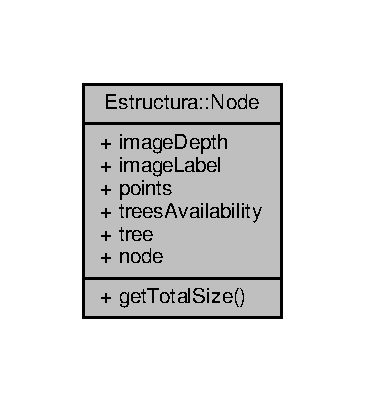
\includegraphics[width=175pt]{structEstructura_1_1Node__coll__graph}
\end{center}
\end{figure}
\subsection*{Public Member Functions}
\begin{DoxyCompactItemize}
\item 
void \hyperlink{structEstructura_1_1Node_a5831e80817a1241fba2de601a9d6fda6}{get\+Total\+Size} (int \&valor)
\end{DoxyCompactItemize}
\subsection*{Public Attributes}
\begin{DoxyCompactItemize}
\item 
cv\+::\+Mat \hyperlink{structEstructura_1_1Node_a117720b249be79aaf71bc0a42d2c9b6b}{image\+Depth}
\item 
cv\+::\+Mat \hyperlink{structEstructura_1_1Node_a7905c0696cb214e84ac855e7a6b6366c}{image\+Label}
\item 
std\+::vector$<$ \hyperlink{structEstructura_1_1Pixel}{Estructura\+::\+Pixel} $>$ \hyperlink{structEstructura_1_1Node_a0ad44a6cbbffdcd39f26733cc0e6f196}{points}
\item 
std\+::vector$<$ int $>$ \hyperlink{structEstructura_1_1Node_aab4eb88cc631cf0829658ca0e7a313a4}{trees\+Availability}
\item 
int \hyperlink{structEstructura_1_1Node_abb400b36a5e8179766c35bc73c22e816}{tree}
\item 
int \hyperlink{structEstructura_1_1Node_a2e360ae2439d4d82dd38d9b30358feac}{node}
\end{DoxyCompactItemize}


\subsection{Member Function Documentation}
\index{Estructura\+::\+Node@{Estructura\+::\+Node}!get\+Total\+Size@{get\+Total\+Size}}
\index{get\+Total\+Size@{get\+Total\+Size}!Estructura\+::\+Node@{Estructura\+::\+Node}}
\subsubsection[{\texorpdfstring{get\+Total\+Size(int \&valor)}{getTotalSize(int &valor)}}]{\setlength{\rightskip}{0pt plus 5cm}void Estructura\+::\+Node\+::get\+Total\+Size (
\begin{DoxyParamCaption}
\item[{int \&}]{valor}
\end{DoxyParamCaption}
)\hspace{0.3cm}{\ttfamily [inline]}}\hypertarget{structEstructura_1_1Node_a5831e80817a1241fba2de601a9d6fda6}{}\label{structEstructura_1_1Node_a5831e80817a1241fba2de601a9d6fda6}


References Estructura\+::node.


\begin{DoxyCode}
40                                      \{
41             valor = \textcolor{keyword}{sizeof}(\hyperlink{structEstructura_1_1Node_a117720b249be79aaf71bc0a42d2c9b6b}{imageDepth}) + \textcolor{keyword}{sizeof}(\hyperlink{structEstructura_1_1Node_a7905c0696cb214e84ac855e7a6b6366c}{imageLabel}) + \textcolor{keyword}{sizeof}(
      \hyperlink{structEstructura_1_1Node_a0ad44a6cbbffdcd39f26733cc0e6f196}{points}) + \textcolor{keyword}{sizeof}(\hyperlink{structEstructura_1_1Node_abb400b36a5e8179766c35bc73c22e816}{tree})+ \textcolor{keyword}{sizeof}(\hyperlink{structEstructura_1_1Node_a2e360ae2439d4d82dd38d9b30358feac}{node});
42         \}
\end{DoxyCode}


\subsection{Member Data Documentation}
\index{Estructura\+::\+Node@{Estructura\+::\+Node}!image\+Depth@{image\+Depth}}
\index{image\+Depth@{image\+Depth}!Estructura\+::\+Node@{Estructura\+::\+Node}}
\subsubsection[{\texorpdfstring{image\+Depth}{imageDepth}}]{\setlength{\rightskip}{0pt plus 5cm}cv\+::\+Mat Estructura\+::\+Node\+::image\+Depth}\hypertarget{structEstructura_1_1Node_a117720b249be79aaf71bc0a42d2c9b6b}{}\label{structEstructura_1_1Node_a117720b249be79aaf71bc0a42d2c9b6b}


Referenced by Image\+::generated\+Structure\+Shotton().

\index{Estructura\+::\+Node@{Estructura\+::\+Node}!image\+Label@{image\+Label}}
\index{image\+Label@{image\+Label}!Estructura\+::\+Node@{Estructura\+::\+Node}}
\subsubsection[{\texorpdfstring{image\+Label}{imageLabel}}]{\setlength{\rightskip}{0pt plus 5cm}cv\+::\+Mat Estructura\+::\+Node\+::image\+Label}\hypertarget{structEstructura_1_1Node_a7905c0696cb214e84ac855e7a6b6366c}{}\label{structEstructura_1_1Node_a7905c0696cb214e84ac855e7a6b6366c}


Referenced by Image\+::generated\+Structure\+Shotton().

\index{Estructura\+::\+Node@{Estructura\+::\+Node}!node@{node}}
\index{node@{node}!Estructura\+::\+Node@{Estructura\+::\+Node}}
\subsubsection[{\texorpdfstring{node}{node}}]{\setlength{\rightskip}{0pt plus 5cm}int Estructura\+::\+Node\+::node}\hypertarget{structEstructura_1_1Node_a2e360ae2439d4d82dd38d9b30358feac}{}\label{structEstructura_1_1Node_a2e360ae2439d4d82dd38d9b30358feac}


Referenced by Image\+::generated\+Structure\+Shotton().

\index{Estructura\+::\+Node@{Estructura\+::\+Node}!points@{points}}
\index{points@{points}!Estructura\+::\+Node@{Estructura\+::\+Node}}
\subsubsection[{\texorpdfstring{points}{points}}]{\setlength{\rightskip}{0pt plus 5cm}std\+::vector$<${\bf Estructura\+::\+Pixel}$>$ Estructura\+::\+Node\+::points}\hypertarget{structEstructura_1_1Node_a0ad44a6cbbffdcd39f26733cc0e6f196}{}\label{structEstructura_1_1Node_a0ad44a6cbbffdcd39f26733cc0e6f196}


Referenced by Image\+::generated\+Structure\+Shotton().

\index{Estructura\+::\+Node@{Estructura\+::\+Node}!tree@{tree}}
\index{tree@{tree}!Estructura\+::\+Node@{Estructura\+::\+Node}}
\subsubsection[{\texorpdfstring{tree}{tree}}]{\setlength{\rightskip}{0pt plus 5cm}int Estructura\+::\+Node\+::tree}\hypertarget{structEstructura_1_1Node_abb400b36a5e8179766c35bc73c22e816}{}\label{structEstructura_1_1Node_abb400b36a5e8179766c35bc73c22e816}


Referenced by Image\+::generated\+Structure\+Shotton().

\index{Estructura\+::\+Node@{Estructura\+::\+Node}!trees\+Availability@{trees\+Availability}}
\index{trees\+Availability@{trees\+Availability}!Estructura\+::\+Node@{Estructura\+::\+Node}}
\subsubsection[{\texorpdfstring{trees\+Availability}{treesAvailability}}]{\setlength{\rightskip}{0pt plus 5cm}std\+::vector$<$int$>$ Estructura\+::\+Node\+::trees\+Availability}\hypertarget{structEstructura_1_1Node_aab4eb88cc631cf0829658ca0e7a313a4}{}\label{structEstructura_1_1Node_aab4eb88cc631cf0829658ca0e7a313a4}


The documentation for this struct was generated from the following file\+:\begin{DoxyCompactItemize}
\item 
\hyperlink{Estructura_8h}{Estructura.\+h}\end{DoxyCompactItemize}

\hypertarget{classrdf_1_1Node}{}\section{rdf\+:\+:Node Class Reference}
\label{classrdf_1_1Node}\index{rdf\+::\+Node@{rdf\+::\+Node}}


{\ttfamily \#include $<$Node.\+h$>$}



Inheritance diagram for rdf\+:\+:Node\+:
\nopagebreak
\begin{figure}[H]
\begin{center}
\leavevmode
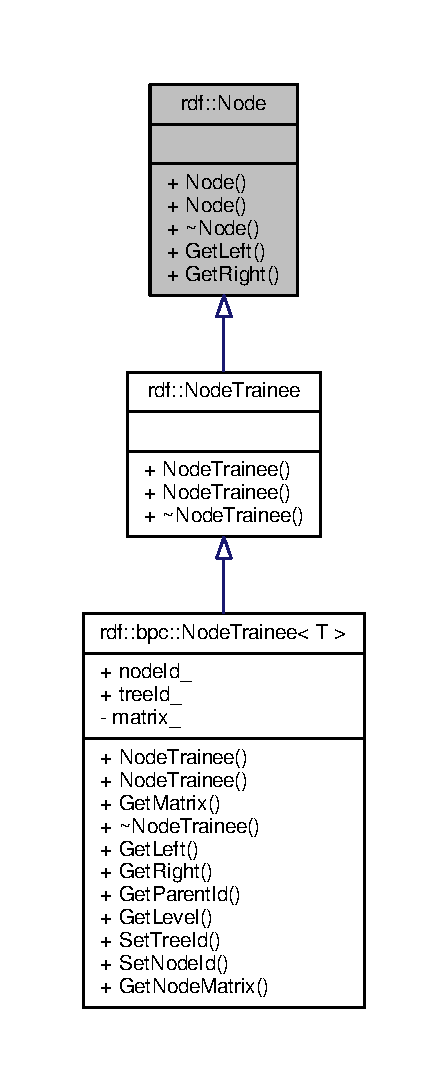
\includegraphics[width=215pt]{classrdf_1_1Node__inherit__graph}
\end{center}
\end{figure}


Collaboration diagram for rdf\+:\+:Node\+:
\nopagebreak
\begin{figure}[H]
\begin{center}
\leavevmode
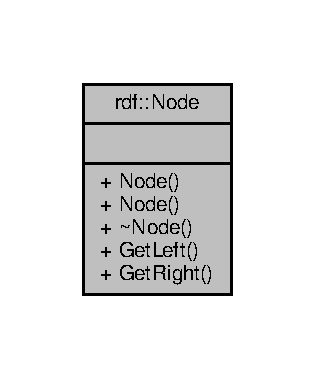
\includegraphics[width=151pt]{classrdf_1_1Node__coll__graph}
\end{center}
\end{figure}
\subsection*{Public Member Functions}
\begin{DoxyCompactItemize}
\item 
\hyperlink{classrdf_1_1Node_ad7a34779cad45d997bfd6d3d8043c75f}{Node} ()
\item 
\hyperlink{classrdf_1_1Node_ab6253a82c82fa130f98d857e277c015e}{Node} (const \hyperlink{classrdf_1_1Node}{Node} \&orig)
\item 
virtual \hyperlink{classrdf_1_1Node_aa0840c3cb5c7159be6d992adecd2097c}{$\sim$\+Node} ()
\item 
virtual \hyperlink{classrdf_1_1Node}{Node} $\ast$ \hyperlink{classrdf_1_1Node_a3957372addb40be853e505359bdda307}{Get\+Left} ()=0
\item 
virtual \hyperlink{classrdf_1_1Node}{Node} $\ast$ \hyperlink{classrdf_1_1Node_a38de220358d574ccc180645d51ae2e06}{Get\+Right} ()=0
\end{DoxyCompactItemize}


\subsection{Constructor \& Destructor Documentation}
\index{rdf\+::\+Node@{rdf\+::\+Node}!Node@{Node}}
\index{Node@{Node}!rdf\+::\+Node@{rdf\+::\+Node}}
\subsubsection[{\texorpdfstring{Node()}{Node()}}]{\setlength{\rightskip}{0pt plus 5cm}Node\+::\+Node (
\begin{DoxyParamCaption}
{}
\end{DoxyParamCaption}
)}\hypertarget{classrdf_1_1Node_ad7a34779cad45d997bfd6d3d8043c75f}{}\label{classrdf_1_1Node_ad7a34779cad45d997bfd6d3d8043c75f}

\begin{DoxyCode}
29            \{
30 \}
\end{DoxyCode}
\index{rdf\+::\+Node@{rdf\+::\+Node}!Node@{Node}}
\index{Node@{Node}!rdf\+::\+Node@{rdf\+::\+Node}}
\subsubsection[{\texorpdfstring{Node(const Node \&orig)}{Node(const Node &orig)}}]{\setlength{\rightskip}{0pt plus 5cm}Node\+::\+Node (
\begin{DoxyParamCaption}
\item[{const {\bf Node} \&}]{orig}
\end{DoxyParamCaption}
)}\hypertarget{classrdf_1_1Node_ab6253a82c82fa130f98d857e277c015e}{}\label{classrdf_1_1Node_ab6253a82c82fa130f98d857e277c015e}

\begin{DoxyCode}
32                            \{
33 \}
\end{DoxyCode}
\index{rdf\+::\+Node@{rdf\+::\+Node}!````~Node@{$\sim$\+Node}}
\index{````~Node@{$\sim$\+Node}!rdf\+::\+Node@{rdf\+::\+Node}}
\subsubsection[{\texorpdfstring{$\sim$\+Node()}{~Node()}}]{\setlength{\rightskip}{0pt plus 5cm}Node\+::$\sim$\+Node (
\begin{DoxyParamCaption}
{}
\end{DoxyParamCaption}
)\hspace{0.3cm}{\ttfamily [virtual]}}\hypertarget{classrdf_1_1Node_aa0840c3cb5c7159be6d992adecd2097c}{}\label{classrdf_1_1Node_aa0840c3cb5c7159be6d992adecd2097c}

\begin{DoxyCode}
35             \{
36 \}
\end{DoxyCode}


\subsection{Member Function Documentation}
\index{rdf\+::\+Node@{rdf\+::\+Node}!Get\+Left@{Get\+Left}}
\index{Get\+Left@{Get\+Left}!rdf\+::\+Node@{rdf\+::\+Node}}
\subsubsection[{\texorpdfstring{Get\+Left()=0}{GetLeft()=0}}]{\setlength{\rightskip}{0pt plus 5cm}virtual {\bf Node}$\ast$ rdf\+::\+Node\+::\+Get\+Left (
\begin{DoxyParamCaption}
{}
\end{DoxyParamCaption}
)\hspace{0.3cm}{\ttfamily [pure virtual]}}\hypertarget{classrdf_1_1Node_a3957372addb40be853e505359bdda307}{}\label{classrdf_1_1Node_a3957372addb40be853e505359bdda307}


Implemented in \hyperlink{classrdf_1_1bpc_1_1NodeTrainee_a36238c22d5235ba77091693343d0b723}{rdf\+::bpc\+::\+Node\+Trainee$<$ T $>$}.

\index{rdf\+::\+Node@{rdf\+::\+Node}!Get\+Right@{Get\+Right}}
\index{Get\+Right@{Get\+Right}!rdf\+::\+Node@{rdf\+::\+Node}}
\subsubsection[{\texorpdfstring{Get\+Right()=0}{GetRight()=0}}]{\setlength{\rightskip}{0pt plus 5cm}virtual {\bf Node}$\ast$ rdf\+::\+Node\+::\+Get\+Right (
\begin{DoxyParamCaption}
{}
\end{DoxyParamCaption}
)\hspace{0.3cm}{\ttfamily [pure virtual]}}\hypertarget{classrdf_1_1Node_a38de220358d574ccc180645d51ae2e06}{}\label{classrdf_1_1Node_a38de220358d574ccc180645d51ae2e06}


Implemented in \hyperlink{classrdf_1_1bpc_1_1NodeTrainee_a5f0aa7a3ba0d742c980215b9be8a9c3c}{rdf\+::bpc\+::\+Node\+Trainee$<$ T $>$}.



The documentation for this class was generated from the following files\+:\begin{DoxyCompactItemize}
\item 
\hyperlink{Node_8h}{Node.\+h}\item 
\hyperlink{Node_8cpp}{Node.\+cpp}\end{DoxyCompactItemize}

\hypertarget{classNodeResource}{}\section{Node\+Resource Class Reference}
\label{classNodeResource}\index{Node\+Resource@{Node\+Resource}}


{\ttfamily \#include $<$Node\+Resource.\+h$>$}



Collaboration diagram for Node\+Resource\+:
\nopagebreak
\begin{figure}[H]
\begin{center}
\leavevmode
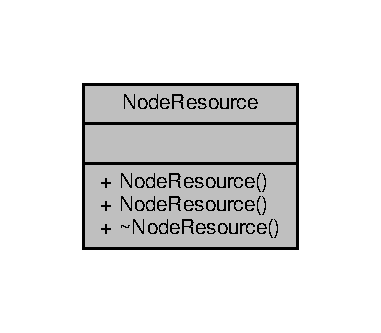
\includegraphics[width=183pt]{classNodeResource__coll__graph}
\end{center}
\end{figure}
\subsection*{Public Member Functions}
\begin{DoxyCompactItemize}
\item 
\hyperlink{classNodeResource_a76b86c3c2f91f79fa76742a44f6ff29b}{Node\+Resource} ()
\item 
\hyperlink{classNodeResource_a4f2dafe758d763950464182920b5250e}{Node\+Resource} (const \hyperlink{classNodeResource}{Node\+Resource} \&orig)
\item 
virtual \hyperlink{classNodeResource_a1a571c36b1305efc198bc273741968f2}{$\sim$\+Node\+Resource} ()
\end{DoxyCompactItemize}


\subsection{Constructor \& Destructor Documentation}
\index{Node\+Resource@{Node\+Resource}!Node\+Resource@{Node\+Resource}}
\index{Node\+Resource@{Node\+Resource}!Node\+Resource@{Node\+Resource}}
\subsubsection[{\texorpdfstring{Node\+Resource()}{NodeResource()}}]{\setlength{\rightskip}{0pt plus 5cm}Node\+Resource\+::\+Node\+Resource (
\begin{DoxyParamCaption}
{}
\end{DoxyParamCaption}
)}\hypertarget{classNodeResource_a76b86c3c2f91f79fa76742a44f6ff29b}{}\label{classNodeResource_a76b86c3c2f91f79fa76742a44f6ff29b}

\begin{DoxyCode}
16                            \{
17 \}
\end{DoxyCode}
\index{Node\+Resource@{Node\+Resource}!Node\+Resource@{Node\+Resource}}
\index{Node\+Resource@{Node\+Resource}!Node\+Resource@{Node\+Resource}}
\subsubsection[{\texorpdfstring{Node\+Resource(const Node\+Resource \&orig)}{NodeResource(const NodeResource &orig)}}]{\setlength{\rightskip}{0pt plus 5cm}Node\+Resource\+::\+Node\+Resource (
\begin{DoxyParamCaption}
\item[{const {\bf Node\+Resource} \&}]{orig}
\end{DoxyParamCaption}
)}\hypertarget{classNodeResource_a4f2dafe758d763950464182920b5250e}{}\label{classNodeResource_a4f2dafe758d763950464182920b5250e}

\begin{DoxyCode}
19                                                    \{
20 \}
\end{DoxyCode}
\index{Node\+Resource@{Node\+Resource}!````~Node\+Resource@{$\sim$\+Node\+Resource}}
\index{````~Node\+Resource@{$\sim$\+Node\+Resource}!Node\+Resource@{Node\+Resource}}
\subsubsection[{\texorpdfstring{$\sim$\+Node\+Resource()}{~NodeResource()}}]{\setlength{\rightskip}{0pt plus 5cm}Node\+Resource\+::$\sim$\+Node\+Resource (
\begin{DoxyParamCaption}
{}
\end{DoxyParamCaption}
)\hspace{0.3cm}{\ttfamily [virtual]}}\hypertarget{classNodeResource_a1a571c36b1305efc198bc273741968f2}{}\label{classNodeResource_a1a571c36b1305efc198bc273741968f2}

\begin{DoxyCode}
22                             \{
23 \}
\end{DoxyCode}


The documentation for this class was generated from the following files\+:\begin{DoxyCompactItemize}
\item 
\hyperlink{NodeResource_8h}{Node\+Resource.\+h}\item 
\hyperlink{NodeResource_8cpp}{Node\+Resource.\+cpp}\end{DoxyCompactItemize}

\hypertarget{classrdf_1_1NodeResult}{}\section{rdf\+:\+:Node\+Result Class Reference}
\label{classrdf_1_1NodeResult}\index{rdf\+::\+Node\+Result@{rdf\+::\+Node\+Result}}


{\ttfamily \#include $<$Node\+Result.\+h$>$}



Collaboration diagram for rdf\+:\+:Node\+Result\+:
\nopagebreak
\begin{figure}[H]
\begin{center}
\leavevmode
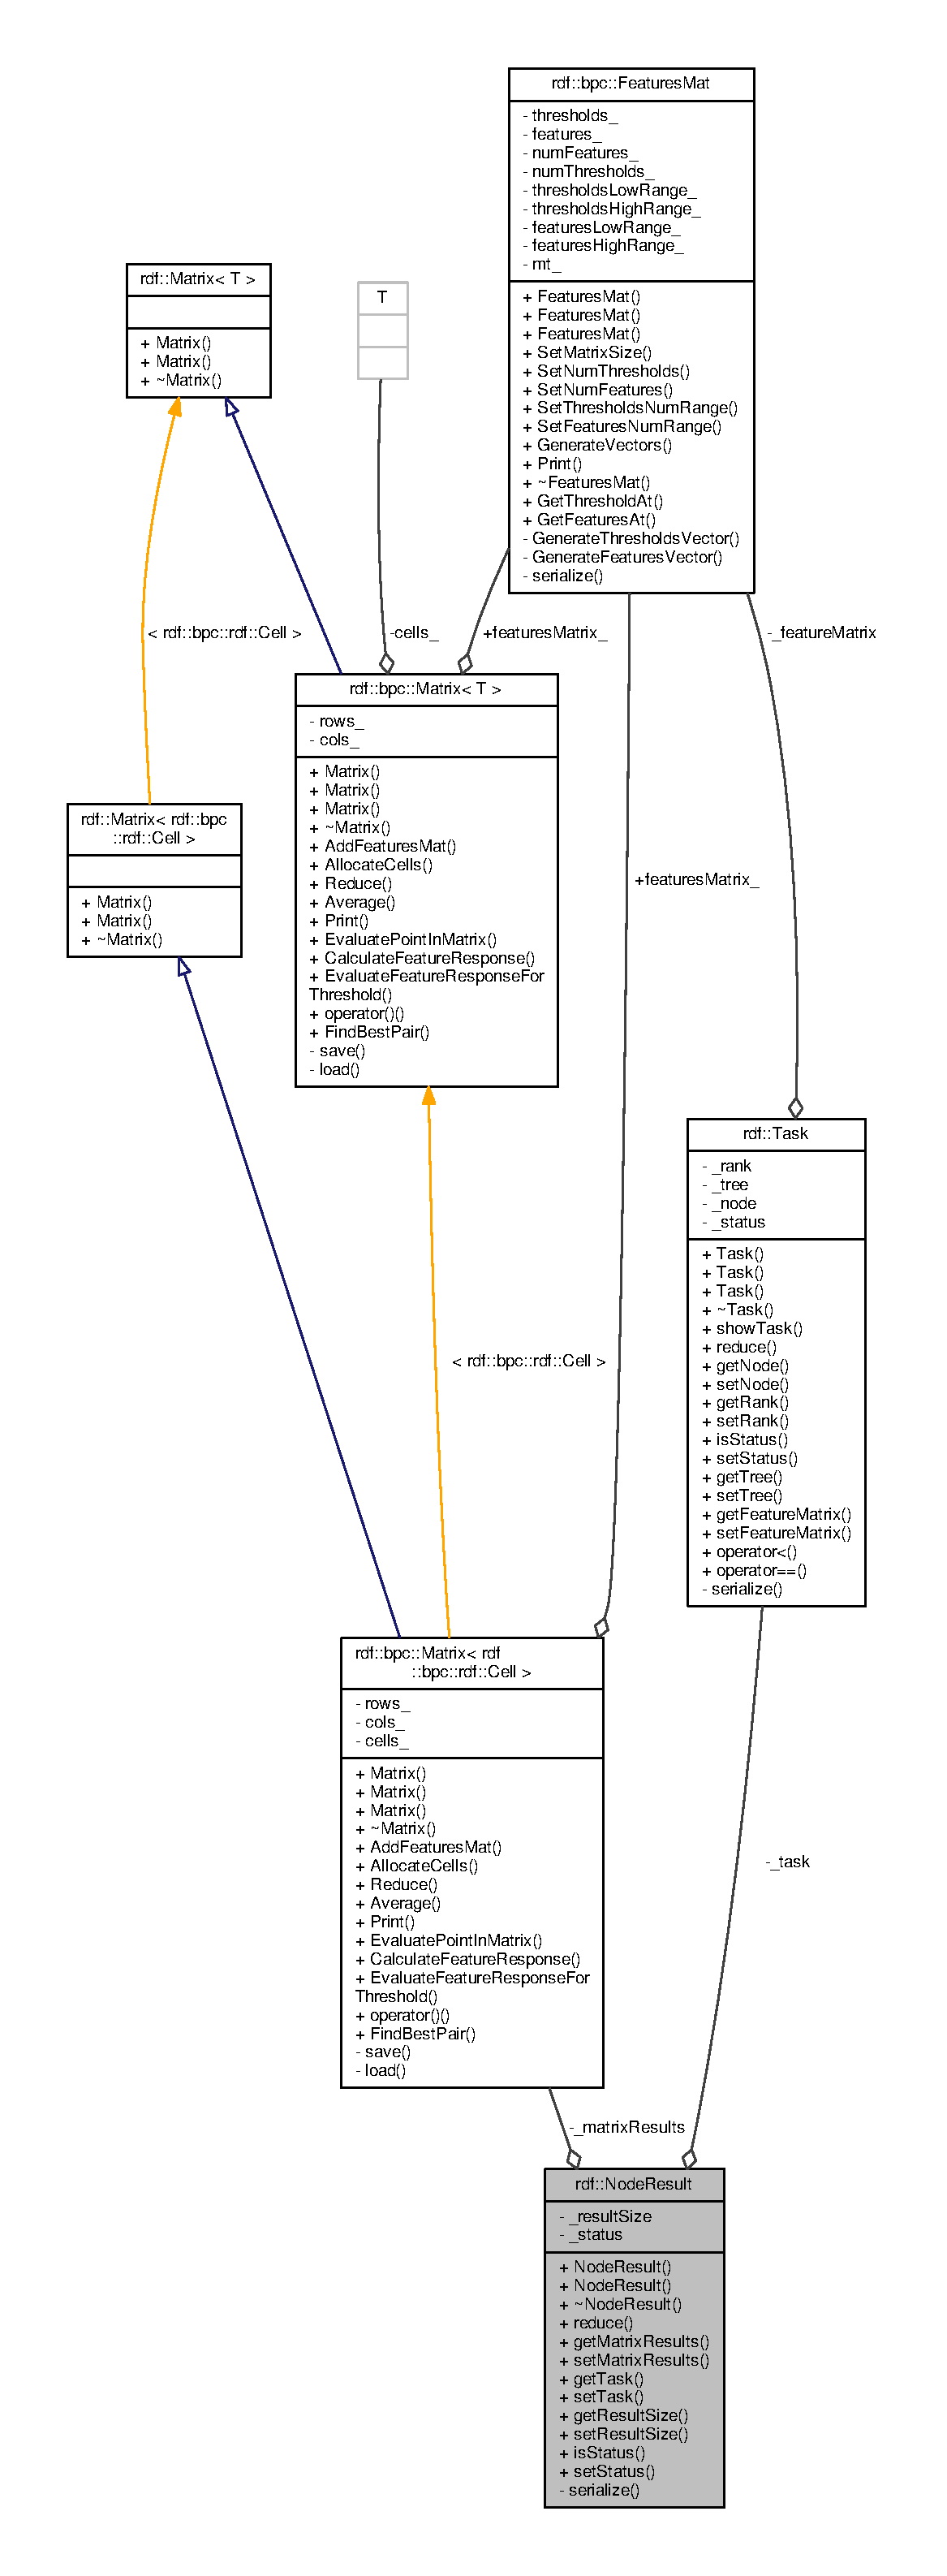
\includegraphics[height=550pt]{classrdf_1_1NodeResult__coll__graph}
\end{center}
\end{figure}
\subsection*{Public Member Functions}
\begin{DoxyCompactItemize}
\item 
\hyperlink{classrdf_1_1NodeResult_ad99a2ab94c710870e623b26a0d735e0c}{Node\+Result} ()
\item 
\hyperlink{classrdf_1_1NodeResult_a4e9bf903b9fc91b519295cf2adee5620}{Node\+Result} (const \hyperlink{classrdf_1_1NodeResult}{Node\+Result} \&orig)
\item 
virtual \hyperlink{classrdf_1_1NodeResult_a949a946b522bb18514b9028ada1c7ed7}{$\sim$\+Node\+Result} ()
\item 
void \hyperlink{classrdf_1_1NodeResult_ac27761fd1c69163c5c9227c0d7fecf92}{reduce} (\hyperlink{classrdf_1_1NodeResult}{Node\+Result} \&Result)
\item 
\hyperlink{classrdf_1_1bpc_1_1Matrix}{rdf\+::bpc\+::\+Matrix}$<$ \hyperlink{classrdf_1_1bpc_1_1Cell}{rdf\+::bpc\+::\+Cell} $>$ \hyperlink{classrdf_1_1NodeResult_ab0d07def4def30c0875602c5e3dde208}{get\+Matrix\+Results} () const 
\item 
void \hyperlink{classrdf_1_1NodeResult_a22523db74203c1926eb1a09da19b5f27}{set\+Matrix\+Results} (\hyperlink{classrdf_1_1bpc_1_1Matrix}{rdf\+::bpc\+::\+Matrix}$<$ \hyperlink{classrdf_1_1bpc_1_1Cell}{rdf\+::bpc\+::\+Cell} $>$ \hyperlink{classrdf_1_1NodeResult_a36b193367d64ea8ca0e71cc912091b71}{\+\_\+matrix\+Results})
\item 
\hyperlink{classrdf_1_1Task}{Task} \hyperlink{classrdf_1_1NodeResult_a564d581492a48333ed9796f6fd4b8c6a}{get\+Task} () const 
\item 
void \hyperlink{classrdf_1_1NodeResult_a29f9794788bb251bccddb5377bb78eba}{set\+Task} (\hyperlink{classrdf_1_1Task}{Task} \hyperlink{classrdf_1_1NodeResult_aa628e795914de688be784892e147fd2d}{\+\_\+task})
\item 
int \hyperlink{classrdf_1_1NodeResult_a47e07daae11352e753629f2fca98d526}{get\+Result\+Size} () const 
\item 
void \hyperlink{classrdf_1_1NodeResult_a8336897151c993416ecb57e2128665b7}{set\+Result\+Size} (int \hyperlink{classrdf_1_1NodeResult_a81eef6ae8527545bc412f49cd3cda6ed}{\+\_\+result\+Size})
\item 
bool \hyperlink{classrdf_1_1NodeResult_a09ad0a96c0591976f73ef288eff195c7}{is\+Status} () const 
\item 
void \hyperlink{classrdf_1_1NodeResult_a52df0a39fb56beec66feacf802639b2c}{set\+Status} (bool \hyperlink{classrdf_1_1NodeResult_a19b142fa64e67d996cb5614450d96c5f}{\+\_\+status})
\end{DoxyCompactItemize}
\subsection*{Private Member Functions}
\begin{DoxyCompactItemize}
\item 
{\footnotesize template$<$class Archive $>$ }\\void \hyperlink{classrdf_1_1NodeResult_a830bc118e64c699ddab67f8a5085ea8f}{serialize} (Archive \&ar, const unsigned int version)
\end{DoxyCompactItemize}
\subsection*{Private Attributes}
\begin{DoxyCompactItemize}
\item 
int \hyperlink{classrdf_1_1NodeResult_a81eef6ae8527545bc412f49cd3cda6ed}{\+\_\+result\+Size} = 0
\item 
bool \hyperlink{classrdf_1_1NodeResult_a19b142fa64e67d996cb5614450d96c5f}{\+\_\+status}
\item 
\hyperlink{classrdf_1_1Task}{rdf\+::\+Task} \hyperlink{classrdf_1_1NodeResult_aa628e795914de688be784892e147fd2d}{\+\_\+task}
\item 
\hyperlink{classrdf_1_1bpc_1_1Matrix}{rdf\+::bpc\+::\+Matrix}$<$ \hyperlink{classrdf_1_1bpc_1_1Cell}{rdf\+::bpc\+::\+Cell} $>$ \hyperlink{classrdf_1_1NodeResult_a36b193367d64ea8ca0e71cc912091b71}{\+\_\+matrix\+Results}
\end{DoxyCompactItemize}
\subsection*{Friends}
\begin{DoxyCompactItemize}
\item 
class \hyperlink{classrdf_1_1NodeResult_ac98d07dd8f7b70e16ccb9a01abf56b9c}{boost\+::serialization\+::access}
\end{DoxyCompactItemize}


\subsection{Constructor \& Destructor Documentation}
\index{rdf\+::\+Node\+Result@{rdf\+::\+Node\+Result}!Node\+Result@{Node\+Result}}
\index{Node\+Result@{Node\+Result}!rdf\+::\+Node\+Result@{rdf\+::\+Node\+Result}}
\subsubsection[{\texorpdfstring{Node\+Result()}{NodeResult()}}]{\setlength{\rightskip}{0pt plus 5cm}rdf\+::\+Node\+Result\+::\+Node\+Result (
\begin{DoxyParamCaption}
{}
\end{DoxyParamCaption}
)}\hypertarget{classrdf_1_1NodeResult_ad99a2ab94c710870e623b26a0d735e0c}{}\label{classrdf_1_1NodeResult_ad99a2ab94c710870e623b26a0d735e0c}

\begin{DoxyCode}
16                           \{
17 \}
\end{DoxyCode}
\index{rdf\+::\+Node\+Result@{rdf\+::\+Node\+Result}!Node\+Result@{Node\+Result}}
\index{Node\+Result@{Node\+Result}!rdf\+::\+Node\+Result@{rdf\+::\+Node\+Result}}
\subsubsection[{\texorpdfstring{Node\+Result(const Node\+Result \&orig)}{NodeResult(const NodeResult &orig)}}]{\setlength{\rightskip}{0pt plus 5cm}rdf\+::\+Node\+Result\+::\+Node\+Result (
\begin{DoxyParamCaption}
\item[{const {\bf Node\+Result} \&}]{orig}
\end{DoxyParamCaption}
)}\hypertarget{classrdf_1_1NodeResult_a4e9bf903b9fc91b519295cf2adee5620}{}\label{classrdf_1_1NodeResult_a4e9bf903b9fc91b519295cf2adee5620}


References \+\_\+matrix\+Results, \+\_\+result\+Size, \+\_\+status, and \+\_\+task.


\begin{DoxyCode}
19                                                 \{
20     \hyperlink{classrdf_1_1NodeResult_a81eef6ae8527545bc412f49cd3cda6ed}{\_resultSize}     = orig.\_resultSize;
21     \hyperlink{classrdf_1_1NodeResult_a19b142fa64e67d996cb5614450d96c5f}{\_status}         = orig.\_status;
22     \hyperlink{classrdf_1_1NodeResult_aa628e795914de688be784892e147fd2d}{\_task}           = orig.\_task;
23     \hyperlink{classrdf_1_1NodeResult_a36b193367d64ea8ca0e71cc912091b71}{\_matrixResults}  = orig.\_matrixResults;
24 \}
\end{DoxyCode}
\index{rdf\+::\+Node\+Result@{rdf\+::\+Node\+Result}!````~Node\+Result@{$\sim$\+Node\+Result}}
\index{````~Node\+Result@{$\sim$\+Node\+Result}!rdf\+::\+Node\+Result@{rdf\+::\+Node\+Result}}
\subsubsection[{\texorpdfstring{$\sim$\+Node\+Result()}{~NodeResult()}}]{\setlength{\rightskip}{0pt plus 5cm}rdf\+::\+Node\+Result\+::$\sim$\+Node\+Result (
\begin{DoxyParamCaption}
{}
\end{DoxyParamCaption}
)\hspace{0.3cm}{\ttfamily [virtual]}}\hypertarget{classrdf_1_1NodeResult_a949a946b522bb18514b9028ada1c7ed7}{}\label{classrdf_1_1NodeResult_a949a946b522bb18514b9028ada1c7ed7}

\begin{DoxyCode}
26                            \{
27 \}
\end{DoxyCode}


\subsection{Member Function Documentation}
\index{rdf\+::\+Node\+Result@{rdf\+::\+Node\+Result}!get\+Matrix\+Results@{get\+Matrix\+Results}}
\index{get\+Matrix\+Results@{get\+Matrix\+Results}!rdf\+::\+Node\+Result@{rdf\+::\+Node\+Result}}
\subsubsection[{\texorpdfstring{get\+Matrix\+Results() const }{getMatrixResults() const }}]{\setlength{\rightskip}{0pt plus 5cm}{\bf rdf\+::bpc\+::\+Matrix}$<${\bf rdf\+::bpc\+::\+Cell}$>$ rdf\+::\+Node\+Result\+::get\+Matrix\+Results (
\begin{DoxyParamCaption}
{}
\end{DoxyParamCaption}
) const\hspace{0.3cm}{\ttfamily [inline]}}\hypertarget{classrdf_1_1NodeResult_ab0d07def4def30c0875602c5e3dde208}{}\label{classrdf_1_1NodeResult_ab0d07def4def30c0875602c5e3dde208}


References \+\_\+matrix\+Results.



Referenced by Scheduler\+::check\+Queues().


\begin{DoxyCode}
57                                                               \{
58                 \textcolor{keywordflow}{return} \hyperlink{classrdf_1_1NodeResult_a36b193367d64ea8ca0e71cc912091b71}{\_matrixResults};
59             \}
\end{DoxyCode}
\index{rdf\+::\+Node\+Result@{rdf\+::\+Node\+Result}!get\+Result\+Size@{get\+Result\+Size}}
\index{get\+Result\+Size@{get\+Result\+Size}!rdf\+::\+Node\+Result@{rdf\+::\+Node\+Result}}
\subsubsection[{\texorpdfstring{get\+Result\+Size() const }{getResultSize() const }}]{\setlength{\rightskip}{0pt plus 5cm}int rdf\+::\+Node\+Result\+::get\+Result\+Size (
\begin{DoxyParamCaption}
{}
\end{DoxyParamCaption}
) const\hspace{0.3cm}{\ttfamily [inline]}}\hypertarget{classrdf_1_1NodeResult_a47e07daae11352e753629f2fca98d526}{}\label{classrdf_1_1NodeResult_a47e07daae11352e753629f2fca98d526}


References \+\_\+result\+Size.



Referenced by rdf\+::\+Forest\+Manager\+::add\+Resuld(), and reduce().


\begin{DoxyCode}
72                                       \{
73                 \textcolor{keywordflow}{return} \hyperlink{classrdf_1_1NodeResult_a81eef6ae8527545bc412f49cd3cda6ed}{\_resultSize};
74             \}
\end{DoxyCode}
\index{rdf\+::\+Node\+Result@{rdf\+::\+Node\+Result}!get\+Task@{get\+Task}}
\index{get\+Task@{get\+Task}!rdf\+::\+Node\+Result@{rdf\+::\+Node\+Result}}
\subsubsection[{\texorpdfstring{get\+Task() const }{getTask() const }}]{\setlength{\rightskip}{0pt plus 5cm}{\bf Task} rdf\+::\+Node\+Result\+::get\+Task (
\begin{DoxyParamCaption}
{}
\end{DoxyParamCaption}
) const\hspace{0.3cm}{\ttfamily [inline]}}\hypertarget{classrdf_1_1NodeResult_a564d581492a48333ed9796f6fd4b8c6a}{}\label{classrdf_1_1NodeResult_a564d581492a48333ed9796f6fd4b8c6a}


References \+\_\+task.



Referenced by rdf\+::\+Forest\+Manager\+::add\+Resuld(), Scheduler\+::check\+Queues(), reduce(), rdf\+::\+Train\+Manager\+::sending\+Results(), and rdf\+::\+Distribution\+Manager\+::waiting\+Results().


\begin{DoxyCode}
65                                  \{
66                 \textcolor{keywordflow}{return} \hyperlink{classrdf_1_1NodeResult_aa628e795914de688be784892e147fd2d}{\_task};
67             \}
\end{DoxyCode}
\index{rdf\+::\+Node\+Result@{rdf\+::\+Node\+Result}!is\+Status@{is\+Status}}
\index{is\+Status@{is\+Status}!rdf\+::\+Node\+Result@{rdf\+::\+Node\+Result}}
\subsubsection[{\texorpdfstring{is\+Status() const }{isStatus() const }}]{\setlength{\rightskip}{0pt plus 5cm}bool rdf\+::\+Node\+Result\+::is\+Status (
\begin{DoxyParamCaption}
{}
\end{DoxyParamCaption}
) const\hspace{0.3cm}{\ttfamily [inline]}}\hypertarget{classrdf_1_1NodeResult_a09ad0a96c0591976f73ef288eff195c7}{}\label{classrdf_1_1NodeResult_a09ad0a96c0591976f73ef288eff195c7}


References \+\_\+status.



Referenced by Scheduler\+::check\+Queues().


\begin{DoxyCode}
80                                   \{
81                 \textcolor{keywordflow}{return} \hyperlink{classrdf_1_1NodeResult_a19b142fa64e67d996cb5614450d96c5f}{\_status};
82             \}
\end{DoxyCode}
\index{rdf\+::\+Node\+Result@{rdf\+::\+Node\+Result}!reduce@{reduce}}
\index{reduce@{reduce}!rdf\+::\+Node\+Result@{rdf\+::\+Node\+Result}}
\subsubsection[{\texorpdfstring{reduce(\+Node\+Result \&\+Result)}{reduce(NodeResult &Result)}}]{\setlength{\rightskip}{0pt plus 5cm}void rdf\+::\+Node\+Result\+::reduce (
\begin{DoxyParamCaption}
\item[{{\bf Node\+Result} \&}]{Result}
\end{DoxyParamCaption}
)}\hypertarget{classrdf_1_1NodeResult_ac27761fd1c69163c5c9227c0d7fecf92}{}\label{classrdf_1_1NodeResult_ac27761fd1c69163c5c9227c0d7fecf92}


References \+\_\+matrix\+Results, \+\_\+result\+Size, \+\_\+status, rdf\+::bpc\+::\+Features\+::feature1\+\_\+, rdf\+::bpc\+::\+Features\+::feature2\+\_\+, rdf\+::\+Task\+::get\+Feature\+Matrix(), rdf\+::bpc\+::\+Features\+Mat\+::\+Get\+Features\+At(), get\+Result\+Size(), get\+Task(), rdf\+::bpc\+::\+Features\+Mat\+::\+Get\+Threshold\+At(), and rdf\+::\+Task\+::show\+Task().


\begin{DoxyCode}
29                                               \{
30     std::cout << \textcolor{stringliteral}{"reducing from "};
31     pResult.getTask().showTask();
32     \hyperlink{classrdf_1_1NodeResult_a36b193367d64ea8ca0e71cc912091b71}{\_matrixResults}.Reduce(pResult.\_matrixResults);
33     
34     std::cout << \textcolor{stringliteral}{" \(\backslash\)n Result left: "} << \hyperlink{classrdf_1_1NodeResult_a81eef6ae8527545bc412f49cd3cda6ed}{\_resultSize}++ << \textcolor{stringliteral}{"\(\backslash\)n"};
35     \textcolor{keywordflow}{if}(\_resultSize == pResult.getResultSize())\{
36         \hyperlink{classrdf_1_1NodeResult_a19b142fa64e67d996cb5614450d96c5f}{\_status} = \textcolor{keyword}{true};
37         std::cout << \textcolor{stringliteral}{"ALL RESULTS from: "};
38         pResult.getTask().showTask();
39         std::pair<int,int> \_featureIndex = pResult.\_matrixResults.FindBestPair();
40         
41         \hyperlink{classrdf_1_1bpc_1_1Features}{rdf::bpc::Features} \_feature   = pResult.getTask().getFeatureMatrix().
      GetFeaturesAt(\_featureIndex.first);
42         \textcolor{keywordtype}{float} \_threshold = pResult.getTask().getFeatureMatrix().GetThresholdAt(\_featureIndex.second);
43         
44         std::cout << \textcolor{stringliteral}{"FEATURES1: "} << \_feature.\hyperlink{classrdf_1_1bpc_1_1Features_a01f4d6cb79311da3b39f82882112bbcb}{feature1\_}.x << \textcolor{stringliteral}{","} << \_feature.
      \hyperlink{classrdf_1_1bpc_1_1Features_a01f4d6cb79311da3b39f82882112bbcb}{feature1\_}.y << \textcolor{stringliteral}{"\(\backslash\)n"};
45         std::cout << \textcolor{stringliteral}{"FEATURES2: "} << \_feature.\hyperlink{classrdf_1_1bpc_1_1Features_a563e43877615b6967a5ec9049bab4b65}{feature2\_}.x << \textcolor{stringliteral}{","} << \_feature.
      \hyperlink{classrdf_1_1bpc_1_1Features_a563e43877615b6967a5ec9049bab4b65}{feature2\_}.y << \textcolor{stringliteral}{"\(\backslash\)n"};
46         std::cout << \textcolor{stringliteral}{"THRESHOLS: "} << \_threshold << \textcolor{stringliteral}{"\(\backslash\)n"};
47     \}
48 \}
\end{DoxyCode}
\index{rdf\+::\+Node\+Result@{rdf\+::\+Node\+Result}!serialize@{serialize}}
\index{serialize@{serialize}!rdf\+::\+Node\+Result@{rdf\+::\+Node\+Result}}
\subsubsection[{\texorpdfstring{serialize(\+Archive \&ar, const unsigned int version)}{serialize(Archive &ar, const unsigned int version)}}]{\setlength{\rightskip}{0pt plus 5cm}template$<$class Archive $>$ void rdf\+::\+Node\+Result\+::serialize (
\begin{DoxyParamCaption}
\item[{Archive \&}]{ar, }
\item[{const unsigned int}]{version}
\end{DoxyParamCaption}
)\hspace{0.3cm}{\ttfamily [inline]}, {\ttfamily [private]}}\hypertarget{classrdf_1_1NodeResult_a830bc118e64c699ddab67f8a5085ea8f}{}\label{classrdf_1_1NodeResult_a830bc118e64c699ddab67f8a5085ea8f}


References \+\_\+matrix\+Results, \+\_\+result\+Size, \+\_\+status, and \+\_\+task.


\begin{DoxyCode}
34             \{
35                 ar & \hyperlink{classrdf_1_1NodeResult_a81eef6ae8527545bc412f49cd3cda6ed}{\_resultSize};
36                 ar & \hyperlink{classrdf_1_1NodeResult_a19b142fa64e67d996cb5614450d96c5f}{\_status};
37                 ar & \hyperlink{classrdf_1_1NodeResult_aa628e795914de688be784892e147fd2d}{\_task};
38                 ar & \hyperlink{classrdf_1_1NodeResult_a36b193367d64ea8ca0e71cc912091b71}{\_matrixResults};
39             \}
\end{DoxyCode}
\index{rdf\+::\+Node\+Result@{rdf\+::\+Node\+Result}!set\+Matrix\+Results@{set\+Matrix\+Results}}
\index{set\+Matrix\+Results@{set\+Matrix\+Results}!rdf\+::\+Node\+Result@{rdf\+::\+Node\+Result}}
\subsubsection[{\texorpdfstring{set\+Matrix\+Results(rdf\+::bpc\+::\+Matrix$<$ rdf\+::bpc\+::\+Cell $>$ \+\_\+matrix\+Results)}{setMatrixResults(rdf::bpc::Matrix< rdf::bpc::Cell > _matrixResults)}}]{\setlength{\rightskip}{0pt plus 5cm}void rdf\+::\+Node\+Result\+::set\+Matrix\+Results (
\begin{DoxyParamCaption}
\item[{{\bf rdf\+::bpc\+::\+Matrix}$<$ {\bf rdf\+::bpc\+::\+Cell} $>$}]{\+\_\+matrix\+Results}
\end{DoxyParamCaption}
)\hspace{0.3cm}{\ttfamily [inline]}}\hypertarget{classrdf_1_1NodeResult_a22523db74203c1926eb1a09da19b5f27}{}\label{classrdf_1_1NodeResult_a22523db74203c1926eb1a09da19b5f27}


References \+\_\+matrix\+Results.



Referenced by rdf\+::bpc\+::\+Trainer\+::\+Train().


\begin{DoxyCode}
61                                                                            \{
62                 this->\_matrixResults = \hyperlink{classrdf_1_1NodeResult_a36b193367d64ea8ca0e71cc912091b71}{\_matrixResults};
63             \}
\end{DoxyCode}
\index{rdf\+::\+Node\+Result@{rdf\+::\+Node\+Result}!set\+Result\+Size@{set\+Result\+Size}}
\index{set\+Result\+Size@{set\+Result\+Size}!rdf\+::\+Node\+Result@{rdf\+::\+Node\+Result}}
\subsubsection[{\texorpdfstring{set\+Result\+Size(int \+\_\+result\+Size)}{setResultSize(int _resultSize)}}]{\setlength{\rightskip}{0pt plus 5cm}void rdf\+::\+Node\+Result\+::set\+Result\+Size (
\begin{DoxyParamCaption}
\item[{int}]{\+\_\+result\+Size}
\end{DoxyParamCaption}
)\hspace{0.3cm}{\ttfamily [inline]}}\hypertarget{classrdf_1_1NodeResult_a8336897151c993416ecb57e2128665b7}{}\label{classrdf_1_1NodeResult_a8336897151c993416ecb57e2128665b7}


References \+\_\+result\+Size.


\begin{DoxyCode}
76                                                 \{
77                 this->\hyperlink{classrdf_1_1NodeResult_a81eef6ae8527545bc412f49cd3cda6ed}{\_resultSize} = \hyperlink{classrdf_1_1NodeResult_a81eef6ae8527545bc412f49cd3cda6ed}{\_resultSize};
78             \}
\end{DoxyCode}
\index{rdf\+::\+Node\+Result@{rdf\+::\+Node\+Result}!set\+Status@{set\+Status}}
\index{set\+Status@{set\+Status}!rdf\+::\+Node\+Result@{rdf\+::\+Node\+Result}}
\subsubsection[{\texorpdfstring{set\+Status(bool \+\_\+status)}{setStatus(bool _status)}}]{\setlength{\rightskip}{0pt plus 5cm}void rdf\+::\+Node\+Result\+::set\+Status (
\begin{DoxyParamCaption}
\item[{bool}]{\+\_\+status}
\end{DoxyParamCaption}
)\hspace{0.3cm}{\ttfamily [inline]}}\hypertarget{classrdf_1_1NodeResult_a52df0a39fb56beec66feacf802639b2c}{}\label{classrdf_1_1NodeResult_a52df0a39fb56beec66feacf802639b2c}


References \+\_\+status.



Referenced by Scheduler\+::check\+Queues().


\begin{DoxyCode}
84                                          \{
85                 this->\hyperlink{classrdf_1_1NodeResult_a19b142fa64e67d996cb5614450d96c5f}{\_status} = \hyperlink{classrdf_1_1NodeResult_a19b142fa64e67d996cb5614450d96c5f}{\_status};
86             \}
\end{DoxyCode}
\index{rdf\+::\+Node\+Result@{rdf\+::\+Node\+Result}!set\+Task@{set\+Task}}
\index{set\+Task@{set\+Task}!rdf\+::\+Node\+Result@{rdf\+::\+Node\+Result}}
\subsubsection[{\texorpdfstring{set\+Task(\+Task \+\_\+task)}{setTask(Task _task)}}]{\setlength{\rightskip}{0pt plus 5cm}void rdf\+::\+Node\+Result\+::set\+Task (
\begin{DoxyParamCaption}
\item[{{\bf Task}}]{\+\_\+task}
\end{DoxyParamCaption}
)\hspace{0.3cm}{\ttfamily [inline]}}\hypertarget{classrdf_1_1NodeResult_a29f9794788bb251bccddb5377bb78eba}{}\label{classrdf_1_1NodeResult_a29f9794788bb251bccddb5377bb78eba}


References \+\_\+task.



Referenced by Scheduler\+::check\+Queues(), and rdf\+::\+Train\+Manager\+::sending\+Results().


\begin{DoxyCode}
69                                      \{
70                 this->\hyperlink{classrdf_1_1NodeResult_aa628e795914de688be784892e147fd2d}{\_task} = \hyperlink{classrdf_1_1NodeResult_aa628e795914de688be784892e147fd2d}{\_task};
71             \}
\end{DoxyCode}


\subsection{Friends And Related Function Documentation}
\index{rdf\+::\+Node\+Result@{rdf\+::\+Node\+Result}!boost\+::serialization\+::access@{boost\+::serialization\+::access}}
\index{boost\+::serialization\+::access@{boost\+::serialization\+::access}!rdf\+::\+Node\+Result@{rdf\+::\+Node\+Result}}
\subsubsection[{\texorpdfstring{boost\+::serialization\+::access}{boost::serialization::access}}]{\setlength{\rightskip}{0pt plus 5cm}friend class boost\+::serialization\+::access\hspace{0.3cm}{\ttfamily [friend]}}\hypertarget{classrdf_1_1NodeResult_ac98d07dd8f7b70e16ccb9a01abf56b9c}{}\label{classrdf_1_1NodeResult_ac98d07dd8f7b70e16ccb9a01abf56b9c}
This class allows to manage information about results of training 

\subsection{Member Data Documentation}
\index{rdf\+::\+Node\+Result@{rdf\+::\+Node\+Result}!\+\_\+matrix\+Results@{\+\_\+matrix\+Results}}
\index{\+\_\+matrix\+Results@{\+\_\+matrix\+Results}!rdf\+::\+Node\+Result@{rdf\+::\+Node\+Result}}
\subsubsection[{\texorpdfstring{\+\_\+matrix\+Results}{_matrixResults}}]{\setlength{\rightskip}{0pt plus 5cm}{\bf rdf\+::bpc\+::\+Matrix}$<${\bf rdf\+::bpc\+::\+Cell}$>$ rdf\+::\+Node\+Result\+::\+\_\+matrix\+Results\hspace{0.3cm}{\ttfamily [private]}}\hypertarget{classrdf_1_1NodeResult_a36b193367d64ea8ca0e71cc912091b71}{}\label{classrdf_1_1NodeResult_a36b193367d64ea8ca0e71cc912091b71}


Referenced by get\+Matrix\+Results(), Node\+Result(), reduce(), serialize(), and set\+Matrix\+Results().

\index{rdf\+::\+Node\+Result@{rdf\+::\+Node\+Result}!\+\_\+result\+Size@{\+\_\+result\+Size}}
\index{\+\_\+result\+Size@{\+\_\+result\+Size}!rdf\+::\+Node\+Result@{rdf\+::\+Node\+Result}}
\subsubsection[{\texorpdfstring{\+\_\+result\+Size}{_resultSize}}]{\setlength{\rightskip}{0pt plus 5cm}int rdf\+::\+Node\+Result\+::\+\_\+result\+Size = 0\hspace{0.3cm}{\ttfamily [private]}}\hypertarget{classrdf_1_1NodeResult_a81eef6ae8527545bc412f49cd3cda6ed}{}\label{classrdf_1_1NodeResult_a81eef6ae8527545bc412f49cd3cda6ed}
To identify the number of results 

Referenced by get\+Result\+Size(), Node\+Result(), reduce(), serialize(), and set\+Result\+Size().

\index{rdf\+::\+Node\+Result@{rdf\+::\+Node\+Result}!\+\_\+status@{\+\_\+status}}
\index{\+\_\+status@{\+\_\+status}!rdf\+::\+Node\+Result@{rdf\+::\+Node\+Result}}
\subsubsection[{\texorpdfstring{\+\_\+status}{_status}}]{\setlength{\rightskip}{0pt plus 5cm}bool rdf\+::\+Node\+Result\+::\+\_\+status\hspace{0.3cm}{\ttfamily [private]}}\hypertarget{classrdf_1_1NodeResult_a19b142fa64e67d996cb5614450d96c5f}{}\label{classrdf_1_1NodeResult_a19b142fa64e67d996cb5614450d96c5f}
To know when all matix had been reduced 

Referenced by is\+Status(), Node\+Result(), reduce(), serialize(), and set\+Status().

\index{rdf\+::\+Node\+Result@{rdf\+::\+Node\+Result}!\+\_\+task@{\+\_\+task}}
\index{\+\_\+task@{\+\_\+task}!rdf\+::\+Node\+Result@{rdf\+::\+Node\+Result}}
\subsubsection[{\texorpdfstring{\+\_\+task}{_task}}]{\setlength{\rightskip}{0pt plus 5cm}{\bf rdf\+::\+Task} rdf\+::\+Node\+Result\+::\+\_\+task\hspace{0.3cm}{\ttfamily [private]}}\hypertarget{classrdf_1_1NodeResult_aa628e795914de688be784892e147fd2d}{}\label{classrdf_1_1NodeResult_aa628e795914de688be784892e147fd2d}
To know which task produce the result 

Referenced by get\+Task(), Node\+Result(), serialize(), and set\+Task().



The documentation for this class was generated from the following files\+:\begin{DoxyCompactItemize}
\item 
\hyperlink{NodeResult_8h}{Node\+Result.\+h}\item 
\hyperlink{NodeResult_8cpp}{Node\+Result.\+cpp}\end{DoxyCompactItemize}

\hypertarget{classrdf_1_1NodeTrainee}{}\section{rdf\+:\+:Node\+Trainee Class Reference}
\label{classrdf_1_1NodeTrainee}\index{rdf\+::\+Node\+Trainee@{rdf\+::\+Node\+Trainee}}


{\ttfamily \#include $<$Node\+Trainee.\+h$>$}



Inheritance diagram for rdf\+:\+:Node\+Trainee\+:
\nopagebreak
\begin{figure}[H]
\begin{center}
\leavevmode
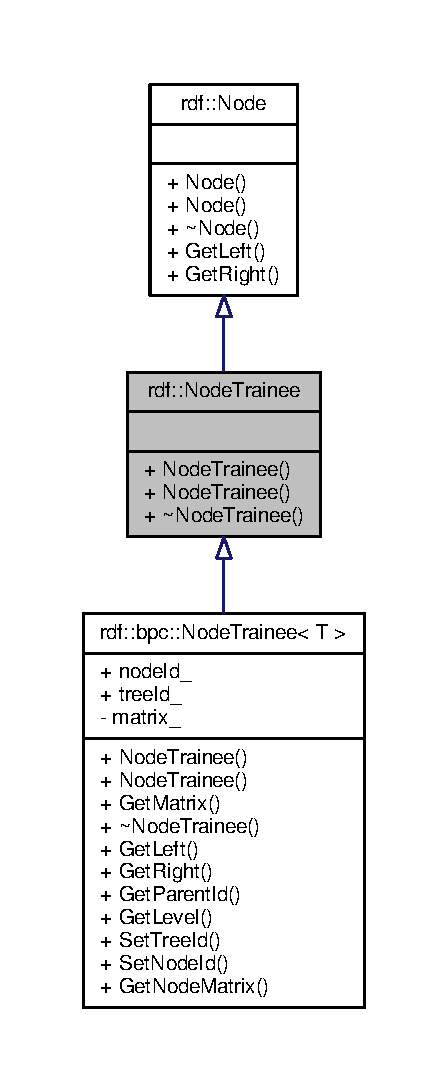
\includegraphics[width=215pt]{classrdf_1_1NodeTrainee__inherit__graph}
\end{center}
\end{figure}


Collaboration diagram for rdf\+:\+:Node\+Trainee\+:
\nopagebreak
\begin{figure}[H]
\begin{center}
\leavevmode
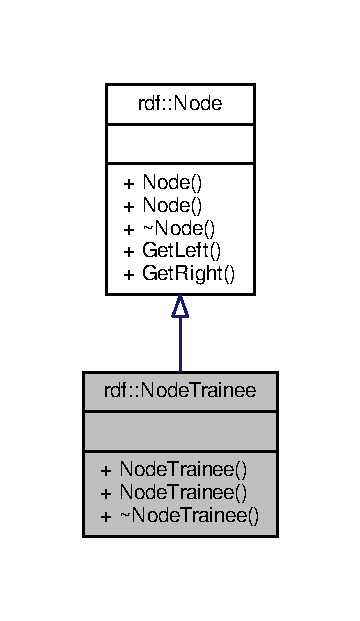
\includegraphics[width=173pt]{classrdf_1_1NodeTrainee__coll__graph}
\end{center}
\end{figure}
\subsection*{Public Member Functions}
\begin{DoxyCompactItemize}
\item 
\hyperlink{classrdf_1_1NodeTrainee_a3a9f61cd118067571d030fcc7aeedad6}{Node\+Trainee} ()
\item 
\hyperlink{classrdf_1_1NodeTrainee_ab696190fee47e73578083694b2a3d6c2}{Node\+Trainee} (const \hyperlink{classrdf_1_1NodeTrainee}{Node\+Trainee} \&orig)
\item 
virtual \hyperlink{classrdf_1_1NodeTrainee_a512115e80d0dbe695be8411a4944325e}{$\sim$\+Node\+Trainee} ()
\end{DoxyCompactItemize}


\subsection{Constructor \& Destructor Documentation}
\index{rdf\+::\+Node\+Trainee@{rdf\+::\+Node\+Trainee}!Node\+Trainee@{Node\+Trainee}}
\index{Node\+Trainee@{Node\+Trainee}!rdf\+::\+Node\+Trainee@{rdf\+::\+Node\+Trainee}}
\subsubsection[{\texorpdfstring{Node\+Trainee()}{NodeTrainee()}}]{\setlength{\rightskip}{0pt plus 5cm}Node\+Trainee\+::\+Node\+Trainee (
\begin{DoxyParamCaption}
{}
\end{DoxyParamCaption}
)}\hypertarget{classrdf_1_1NodeTrainee_a3a9f61cd118067571d030fcc7aeedad6}{}\label{classrdf_1_1NodeTrainee_a3a9f61cd118067571d030fcc7aeedad6}

\begin{DoxyCode}
29                          \{
30 \}
\end{DoxyCode}
\index{rdf\+::\+Node\+Trainee@{rdf\+::\+Node\+Trainee}!Node\+Trainee@{Node\+Trainee}}
\index{Node\+Trainee@{Node\+Trainee}!rdf\+::\+Node\+Trainee@{rdf\+::\+Node\+Trainee}}
\subsubsection[{\texorpdfstring{Node\+Trainee(const Node\+Trainee \&orig)}{NodeTrainee(const NodeTrainee &orig)}}]{\setlength{\rightskip}{0pt plus 5cm}Node\+Trainee\+::\+Node\+Trainee (
\begin{DoxyParamCaption}
\item[{const {\bf Node\+Trainee} \&}]{orig}
\end{DoxyParamCaption}
)}\hypertarget{classrdf_1_1NodeTrainee_ab696190fee47e73578083694b2a3d6c2}{}\label{classrdf_1_1NodeTrainee_ab696190fee47e73578083694b2a3d6c2}

\begin{DoxyCode}
32                                                 \{
33 \}
\end{DoxyCode}
\index{rdf\+::\+Node\+Trainee@{rdf\+::\+Node\+Trainee}!````~Node\+Trainee@{$\sim$\+Node\+Trainee}}
\index{````~Node\+Trainee@{$\sim$\+Node\+Trainee}!rdf\+::\+Node\+Trainee@{rdf\+::\+Node\+Trainee}}
\subsubsection[{\texorpdfstring{$\sim$\+Node\+Trainee()}{~NodeTrainee()}}]{\setlength{\rightskip}{0pt plus 5cm}Node\+Trainee\+::$\sim$\+Node\+Trainee (
\begin{DoxyParamCaption}
{}
\end{DoxyParamCaption}
)\hspace{0.3cm}{\ttfamily [virtual]}}\hypertarget{classrdf_1_1NodeTrainee_a512115e80d0dbe695be8411a4944325e}{}\label{classrdf_1_1NodeTrainee_a512115e80d0dbe695be8411a4944325e}


Reimplemented in \hyperlink{classrdf_1_1bpc_1_1NodeTrainee_a952e836bd65a9219a3ec03b3c6935583}{rdf\+::bpc\+::\+Node\+Trainee$<$ T $>$}.


\begin{DoxyCode}
35                           \{
36 \}
\end{DoxyCode}


The documentation for this class was generated from the following files\+:\begin{DoxyCompactItemize}
\item 
\hyperlink{NodeTrainee_8h}{Node\+Trainee.\+h}\item 
\hyperlink{NodeTrainee_8cpp}{Node\+Trainee.\+cpp}\end{DoxyCompactItemize}

\hypertarget{classrdf_1_1bpc_1_1NodeTrainee}{}\section{rdf\+:\+:bpc\+:\+:Node\+Trainee$<$ T $>$ Class Template Reference}
\label{classrdf_1_1bpc_1_1NodeTrainee}\index{rdf\+::bpc\+::\+Node\+Trainee$<$ T $>$@{rdf\+::bpc\+::\+Node\+Trainee$<$ T $>$}}


{\ttfamily \#include $<$Node\+Trainee\+B\+P\+C.\+h$>$}



Inheritance diagram for rdf\+:\+:bpc\+:\+:Node\+Trainee$<$ T $>$\+:
\nopagebreak
\begin{figure}[H]
\begin{center}
\leavevmode
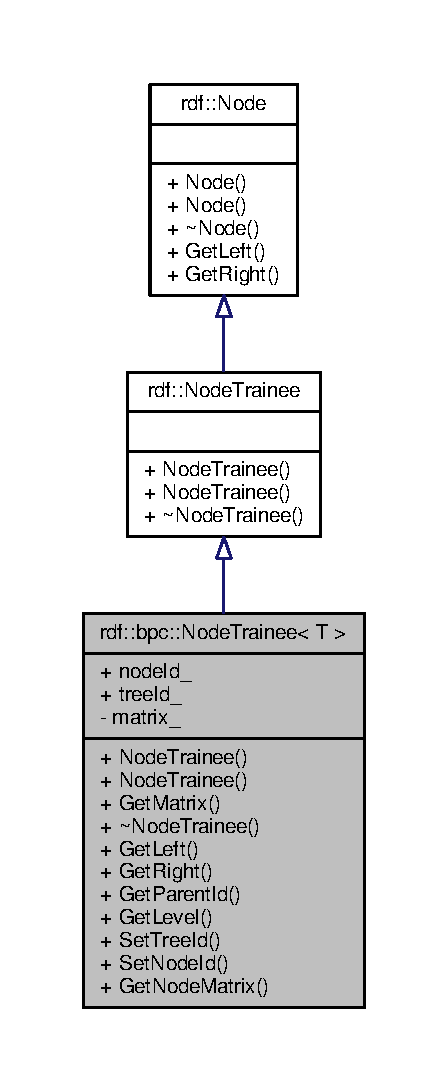
\includegraphics[width=215pt]{classrdf_1_1bpc_1_1NodeTrainee__inherit__graph}
\end{center}
\end{figure}


Collaboration diagram for rdf\+:\+:bpc\+:\+:Node\+Trainee$<$ T $>$\+:
\nopagebreak
\begin{figure}[H]
\begin{center}
\leavevmode
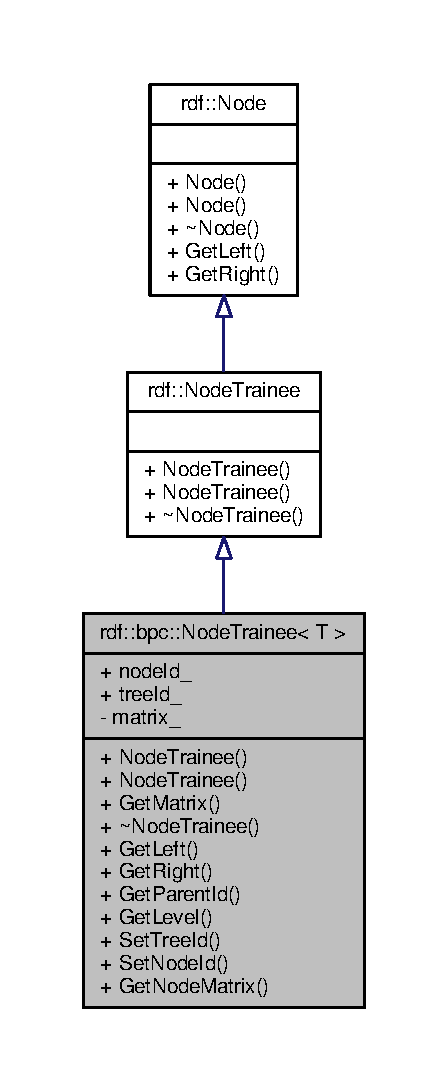
\includegraphics[width=215pt]{classrdf_1_1bpc_1_1NodeTrainee__coll__graph}
\end{center}
\end{figure}
\subsection*{Public Member Functions}
\begin{DoxyCompactItemize}
\item 
\hyperlink{classrdf_1_1bpc_1_1NodeTrainee_a2c076c9286a88ce049e4e6c8707e32ba}{Node\+Trainee} ()
\item 
\hyperlink{classrdf_1_1bpc_1_1NodeTrainee_a0b8bb46d5559d8f665e73b3284e4a615}{Node\+Trainee} (const \hyperlink{classrdf_1_1bpc_1_1NodeTrainee}{Node\+Trainee} \&orig)
\item 
\hyperlink{classrdf_1_1bpc_1_1Matrix}{Matrix}$<$ T $>$ \& \hyperlink{classrdf_1_1bpc_1_1NodeTrainee_ab1ae16941f52a5f38e438b13ed3cee53}{Get\+Matrix} ()
\item 
virtual \hyperlink{classrdf_1_1bpc_1_1NodeTrainee_a952e836bd65a9219a3ec03b3c6935583}{$\sim$\+Node\+Trainee} ()
\item 
\hyperlink{classrdf_1_1Node}{Node} $\ast$ \hyperlink{classrdf_1_1bpc_1_1NodeTrainee_a36238c22d5235ba77091693343d0b723}{Get\+Left} ()
\item 
\hyperlink{classrdf_1_1Node}{Node} $\ast$ \hyperlink{classrdf_1_1bpc_1_1NodeTrainee_a5f0aa7a3ba0d742c980215b9be8a9c3c}{Get\+Right} ()
\item 
int \hyperlink{classrdf_1_1bpc_1_1NodeTrainee_a9d46183bfc982ccb802f7d3e47d109dc}{Get\+Parent\+Id} ()
\item 
int \hyperlink{classrdf_1_1bpc_1_1NodeTrainee_acc58b2d13c5e637938ac7a8934a739bb}{Get\+Level} ()
\item 
void \hyperlink{classrdf_1_1bpc_1_1NodeTrainee_af7bb9c9df89101c4911fe9713ed6aff5}{Set\+Tree\+Id} (int id)
\item 
void \hyperlink{classrdf_1_1bpc_1_1NodeTrainee_a6c42d9a2911c014addb9c5021a484085}{Set\+Node\+Id} (int id)
\item 
\hyperlink{classrdf_1_1bpc_1_1Matrix}{Matrix}$<$ T $>$ \hyperlink{classrdf_1_1bpc_1_1NodeTrainee_aa1879ed3aa007bb3d67cdea5ddbaa45f}{Get\+Node\+Matrix} ()
\end{DoxyCompactItemize}
\subsection*{Public Attributes}
\begin{DoxyCompactItemize}
\item 
int \hyperlink{classrdf_1_1bpc_1_1NodeTrainee_a208e3eafbece621b9618f6e3ddd27947}{node\+Id\+\_\+}
\item 
int \hyperlink{classrdf_1_1bpc_1_1NodeTrainee_a04ec4bdb96ed7d47ab99e6a4f65294f3}{tree\+Id\+\_\+}
\end{DoxyCompactItemize}
\subsection*{Private Attributes}
\begin{DoxyCompactItemize}
\item 
\hyperlink{classrdf_1_1bpc_1_1Matrix}{Matrix}$<$ T $>$ \hyperlink{classrdf_1_1bpc_1_1NodeTrainee_af5b2daa1f044078d5086200e43ae9b0f}{matrix\+\_\+}
\end{DoxyCompactItemize}


\subsection{Constructor \& Destructor Documentation}
\index{rdf\+::bpc\+::\+Node\+Trainee@{rdf\+::bpc\+::\+Node\+Trainee}!Node\+Trainee@{Node\+Trainee}}
\index{Node\+Trainee@{Node\+Trainee}!rdf\+::bpc\+::\+Node\+Trainee@{rdf\+::bpc\+::\+Node\+Trainee}}
\subsubsection[{\texorpdfstring{Node\+Trainee()}{NodeTrainee()}}]{\setlength{\rightskip}{0pt plus 5cm}template$<$typename T$>$ {\bf rdf\+::bpc\+::\+Node\+Trainee}$<$ T $>$\+::{\bf Node\+Trainee} (
\begin{DoxyParamCaption}
{}
\end{DoxyParamCaption}
)}\hypertarget{classrdf_1_1bpc_1_1NodeTrainee_a2c076c9286a88ce049e4e6c8707e32ba}{}\label{classrdf_1_1bpc_1_1NodeTrainee_a2c076c9286a88ce049e4e6c8707e32ba}
\index{rdf\+::bpc\+::\+Node\+Trainee@{rdf\+::bpc\+::\+Node\+Trainee}!Node\+Trainee@{Node\+Trainee}}
\index{Node\+Trainee@{Node\+Trainee}!rdf\+::bpc\+::\+Node\+Trainee@{rdf\+::bpc\+::\+Node\+Trainee}}
\subsubsection[{\texorpdfstring{Node\+Trainee(const Node\+Trainee \&orig)}{NodeTrainee(const NodeTrainee &orig)}}]{\setlength{\rightskip}{0pt plus 5cm}template$<$typename T$>$ {\bf rdf\+::bpc\+::\+Node\+Trainee}$<$ T $>$\+::{\bf Node\+Trainee} (
\begin{DoxyParamCaption}
\item[{const {\bf Node\+Trainee}$<$ T $>$ \&}]{orig}
\end{DoxyParamCaption}
)}\hypertarget{classrdf_1_1bpc_1_1NodeTrainee_a0b8bb46d5559d8f665e73b3284e4a615}{}\label{classrdf_1_1bpc_1_1NodeTrainee_a0b8bb46d5559d8f665e73b3284e4a615}
\index{rdf\+::bpc\+::\+Node\+Trainee@{rdf\+::bpc\+::\+Node\+Trainee}!````~Node\+Trainee@{$\sim$\+Node\+Trainee}}
\index{````~Node\+Trainee@{$\sim$\+Node\+Trainee}!rdf\+::bpc\+::\+Node\+Trainee@{rdf\+::bpc\+::\+Node\+Trainee}}
\subsubsection[{\texorpdfstring{$\sim$\+Node\+Trainee()}{~NodeTrainee()}}]{\setlength{\rightskip}{0pt plus 5cm}template$<$typename T$>$ virtual {\bf rdf\+::bpc\+::\+Node\+Trainee}$<$ T $>$\+::$\sim${\bf Node\+Trainee} (
\begin{DoxyParamCaption}
{}
\end{DoxyParamCaption}
)\hspace{0.3cm}{\ttfamily [virtual]}}\hypertarget{classrdf_1_1bpc_1_1NodeTrainee_a952e836bd65a9219a3ec03b3c6935583}{}\label{classrdf_1_1bpc_1_1NodeTrainee_a952e836bd65a9219a3ec03b3c6935583}


Reimplemented from \hyperlink{classrdf_1_1NodeTrainee_a512115e80d0dbe695be8411a4944325e}{rdf\+::\+Node\+Trainee}.



Referenced by rdf\+::bpc\+::\+Node\+Trainee$<$ T $>$\+::\+Get\+Matrix().



\subsection{Member Function Documentation}
\index{rdf\+::bpc\+::\+Node\+Trainee@{rdf\+::bpc\+::\+Node\+Trainee}!Get\+Left@{Get\+Left}}
\index{Get\+Left@{Get\+Left}!rdf\+::bpc\+::\+Node\+Trainee@{rdf\+::bpc\+::\+Node\+Trainee}}
\subsubsection[{\texorpdfstring{Get\+Left()}{GetLeft()}}]{\setlength{\rightskip}{0pt plus 5cm}template$<$typename T$>$ {\bf Node}$\ast$ {\bf rdf\+::bpc\+::\+Node\+Trainee}$<$ T $>$\+::Get\+Left (
\begin{DoxyParamCaption}
{}
\end{DoxyParamCaption}
)\hspace{0.3cm}{\ttfamily [inline]}, {\ttfamily [virtual]}}\hypertarget{classrdf_1_1bpc_1_1NodeTrainee_a36238c22d5235ba77091693343d0b723}{}\label{classrdf_1_1bpc_1_1NodeTrainee_a36238c22d5235ba77091693343d0b723}


Implements \hyperlink{classrdf_1_1Node_a3957372addb40be853e505359bdda307}{rdf\+::\+Node}.


\begin{DoxyCode}
42 \{\};
\end{DoxyCode}
\index{rdf\+::bpc\+::\+Node\+Trainee@{rdf\+::bpc\+::\+Node\+Trainee}!Get\+Level@{Get\+Level}}
\index{Get\+Level@{Get\+Level}!rdf\+::bpc\+::\+Node\+Trainee@{rdf\+::bpc\+::\+Node\+Trainee}}
\subsubsection[{\texorpdfstring{Get\+Level()}{GetLevel()}}]{\setlength{\rightskip}{0pt plus 5cm}template$<$typename T$>$ int {\bf rdf\+::bpc\+::\+Node\+Trainee}$<$ T $>$\+::Get\+Level (
\begin{DoxyParamCaption}
{}
\end{DoxyParamCaption}
)}\hypertarget{classrdf_1_1bpc_1_1NodeTrainee_acc58b2d13c5e637938ac7a8934a739bb}{}\label{classrdf_1_1bpc_1_1NodeTrainee_acc58b2d13c5e637938ac7a8934a739bb}


Referenced by rdf\+::bpc\+::\+Node\+Trainee$<$ T $>$\+::\+Get\+Parent\+Id().

\index{rdf\+::bpc\+::\+Node\+Trainee@{rdf\+::bpc\+::\+Node\+Trainee}!Get\+Matrix@{Get\+Matrix}}
\index{Get\+Matrix@{Get\+Matrix}!rdf\+::bpc\+::\+Node\+Trainee@{rdf\+::bpc\+::\+Node\+Trainee}}
\subsubsection[{\texorpdfstring{Get\+Matrix()}{GetMatrix()}}]{\setlength{\rightskip}{0pt plus 5cm}template$<$typename T$>$ {\bf Matrix}$<$T$>$\& {\bf rdf\+::bpc\+::\+Node\+Trainee}$<$ T $>$\+::Get\+Matrix (
\begin{DoxyParamCaption}
{}
\end{DoxyParamCaption}
)\hspace{0.3cm}{\ttfamily [inline]}}\hypertarget{classrdf_1_1bpc_1_1NodeTrainee_ab1ae16941f52a5f38e438b13ed3cee53}{}\label{classrdf_1_1bpc_1_1NodeTrainee_ab1ae16941f52a5f38e438b13ed3cee53}


References rdf\+::bpc\+::\+Node\+Trainee$<$ T $>$\+::matrix\+\_\+, and rdf\+::bpc\+::\+Node\+Trainee$<$ T $>$\+::$\sim$\+Node\+Trainee().



Referenced by init(), Queue\+Thread\+::run(), and rdf\+::bpc\+::\+Trainer\+::\+Train().


\begin{DoxyCode}
40 \{ \textcolor{keywordflow}{return} this->\hyperlink{classrdf_1_1bpc_1_1NodeTrainee_af5b2daa1f044078d5086200e43ae9b0f}{matrix\_}; \};
\end{DoxyCode}
\index{rdf\+::bpc\+::\+Node\+Trainee@{rdf\+::bpc\+::\+Node\+Trainee}!Get\+Node\+Matrix@{Get\+Node\+Matrix}}
\index{Get\+Node\+Matrix@{Get\+Node\+Matrix}!rdf\+::bpc\+::\+Node\+Trainee@{rdf\+::bpc\+::\+Node\+Trainee}}
\subsubsection[{\texorpdfstring{Get\+Node\+Matrix()}{GetNodeMatrix()}}]{\setlength{\rightskip}{0pt plus 5cm}template$<$typename T$>$ {\bf Matrix}$<$T$>$ {\bf rdf\+::bpc\+::\+Node\+Trainee}$<$ T $>$\+::Get\+Node\+Matrix (
\begin{DoxyParamCaption}
{}
\end{DoxyParamCaption}
)\hspace{0.3cm}{\ttfamily [inline]}}\hypertarget{classrdf_1_1bpc_1_1NodeTrainee_aa1879ed3aa007bb3d67cdea5ddbaa45f}{}\label{classrdf_1_1bpc_1_1NodeTrainee_aa1879ed3aa007bb3d67cdea5ddbaa45f}


References rdf\+::bpc\+::\+Node\+Trainee$<$ T $>$\+::matrix\+\_\+.


\begin{DoxyCode}
52                                       \{
53         \textcolor{keywordflow}{return} \hyperlink{classrdf_1_1bpc_1_1NodeTrainee_af5b2daa1f044078d5086200e43ae9b0f}{matrix\_};
54       \}
\end{DoxyCode}
\index{rdf\+::bpc\+::\+Node\+Trainee@{rdf\+::bpc\+::\+Node\+Trainee}!Get\+Parent\+Id@{Get\+Parent\+Id}}
\index{Get\+Parent\+Id@{Get\+Parent\+Id}!rdf\+::bpc\+::\+Node\+Trainee@{rdf\+::bpc\+::\+Node\+Trainee}}
\subsubsection[{\texorpdfstring{Get\+Parent\+Id()}{GetParentId()}}]{\setlength{\rightskip}{0pt plus 5cm}template$<$typename T$>$ int {\bf rdf\+::bpc\+::\+Node\+Trainee}$<$ T $>$\+::Get\+Parent\+Id (
\begin{DoxyParamCaption}
{}
\end{DoxyParamCaption}
)\hspace{0.3cm}{\ttfamily [inline]}}\hypertarget{classrdf_1_1bpc_1_1NodeTrainee_a9d46183bfc982ccb802f7d3e47d109dc}{}\label{classrdf_1_1bpc_1_1NodeTrainee_a9d46183bfc982ccb802f7d3e47d109dc}


References rdf\+::bpc\+::\+Node\+Trainee$<$ T $>$\+::\+Get\+Level(), and rdf\+::bpc\+::\+Node\+Trainee$<$ T $>$\+::node\+Id\+\_\+.


\begin{DoxyCode}
44 \{ \textcolor{keywordflow}{return} \hyperlink{classrdf_1_1bpc_1_1NodeTrainee_a208e3eafbece621b9618f6e3ddd27947}{nodeId\_} >> 1; \}
\end{DoxyCode}
\index{rdf\+::bpc\+::\+Node\+Trainee@{rdf\+::bpc\+::\+Node\+Trainee}!Get\+Right@{Get\+Right}}
\index{Get\+Right@{Get\+Right}!rdf\+::bpc\+::\+Node\+Trainee@{rdf\+::bpc\+::\+Node\+Trainee}}
\subsubsection[{\texorpdfstring{Get\+Right()}{GetRight()}}]{\setlength{\rightskip}{0pt plus 5cm}template$<$typename T$>$ {\bf Node}$\ast$ {\bf rdf\+::bpc\+::\+Node\+Trainee}$<$ T $>$\+::Get\+Right (
\begin{DoxyParamCaption}
{}
\end{DoxyParamCaption}
)\hspace{0.3cm}{\ttfamily [inline]}, {\ttfamily [virtual]}}\hypertarget{classrdf_1_1bpc_1_1NodeTrainee_a5f0aa7a3ba0d742c980215b9be8a9c3c}{}\label{classrdf_1_1bpc_1_1NodeTrainee_a5f0aa7a3ba0d742c980215b9be8a9c3c}


Implements \hyperlink{classrdf_1_1Node_a38de220358d574ccc180645d51ae2e06}{rdf\+::\+Node}.


\begin{DoxyCode}
43 \{\};
\end{DoxyCode}
\index{rdf\+::bpc\+::\+Node\+Trainee@{rdf\+::bpc\+::\+Node\+Trainee}!Set\+Node\+Id@{Set\+Node\+Id}}
\index{Set\+Node\+Id@{Set\+Node\+Id}!rdf\+::bpc\+::\+Node\+Trainee@{rdf\+::bpc\+::\+Node\+Trainee}}
\subsubsection[{\texorpdfstring{Set\+Node\+Id(int id)}{SetNodeId(int id)}}]{\setlength{\rightskip}{0pt plus 5cm}template$<$typename T$>$ void {\bf rdf\+::bpc\+::\+Node\+Trainee}$<$ T $>$\+::Set\+Node\+Id (
\begin{DoxyParamCaption}
\item[{int}]{id}
\end{DoxyParamCaption}
)\hspace{0.3cm}{\ttfamily [inline]}}\hypertarget{classrdf_1_1bpc_1_1NodeTrainee_a6c42d9a2911c014addb9c5021a484085}{}\label{classrdf_1_1bpc_1_1NodeTrainee_a6c42d9a2911c014addb9c5021a484085}


References rdf\+::bpc\+::\+Node\+Trainee$<$ T $>$\+::node\+Id\+\_\+.



Referenced by init(), and Queue\+Thread\+::run().


\begin{DoxyCode}
49                                    \{
50         \hyperlink{classrdf_1_1bpc_1_1NodeTrainee_a208e3eafbece621b9618f6e3ddd27947}{nodeId\_} = id;
51       \}
\end{DoxyCode}
\index{rdf\+::bpc\+::\+Node\+Trainee@{rdf\+::bpc\+::\+Node\+Trainee}!Set\+Tree\+Id@{Set\+Tree\+Id}}
\index{Set\+Tree\+Id@{Set\+Tree\+Id}!rdf\+::bpc\+::\+Node\+Trainee@{rdf\+::bpc\+::\+Node\+Trainee}}
\subsubsection[{\texorpdfstring{Set\+Tree\+Id(int id)}{SetTreeId(int id)}}]{\setlength{\rightskip}{0pt plus 5cm}template$<$typename T$>$ void {\bf rdf\+::bpc\+::\+Node\+Trainee}$<$ T $>$\+::Set\+Tree\+Id (
\begin{DoxyParamCaption}
\item[{int}]{id}
\end{DoxyParamCaption}
)\hspace{0.3cm}{\ttfamily [inline]}}\hypertarget{classrdf_1_1bpc_1_1NodeTrainee_af7bb9c9df89101c4911fe9713ed6aff5}{}\label{classrdf_1_1bpc_1_1NodeTrainee_af7bb9c9df89101c4911fe9713ed6aff5}


References rdf\+::bpc\+::\+Node\+Trainee$<$ T $>$\+::tree\+Id\+\_\+.



Referenced by init(), and Queue\+Thread\+::run().


\begin{DoxyCode}
46                                    \{
47         \hyperlink{classrdf_1_1bpc_1_1NodeTrainee_a04ec4bdb96ed7d47ab99e6a4f65294f3}{treeId\_} = id;
48       \}
\end{DoxyCode}


\subsection{Member Data Documentation}
\index{rdf\+::bpc\+::\+Node\+Trainee@{rdf\+::bpc\+::\+Node\+Trainee}!matrix\+\_\+@{matrix\+\_\+}}
\index{matrix\+\_\+@{matrix\+\_\+}!rdf\+::bpc\+::\+Node\+Trainee@{rdf\+::bpc\+::\+Node\+Trainee}}
\subsubsection[{\texorpdfstring{matrix\+\_\+}{matrix_}}]{\setlength{\rightskip}{0pt plus 5cm}template$<$typename T$>$ {\bf Matrix}$<$T$>$ {\bf rdf\+::bpc\+::\+Node\+Trainee}$<$ T $>$\+::matrix\+\_\+\hspace{0.3cm}{\ttfamily [private]}}\hypertarget{classrdf_1_1bpc_1_1NodeTrainee_af5b2daa1f044078d5086200e43ae9b0f}{}\label{classrdf_1_1bpc_1_1NodeTrainee_af5b2daa1f044078d5086200e43ae9b0f}


Referenced by rdf\+::bpc\+::\+Node\+Trainee$<$ T $>$\+::\+Get\+Matrix(), and rdf\+::bpc\+::\+Node\+Trainee$<$ T $>$\+::\+Get\+Node\+Matrix().

\index{rdf\+::bpc\+::\+Node\+Trainee@{rdf\+::bpc\+::\+Node\+Trainee}!node\+Id\+\_\+@{node\+Id\+\_\+}}
\index{node\+Id\+\_\+@{node\+Id\+\_\+}!rdf\+::bpc\+::\+Node\+Trainee@{rdf\+::bpc\+::\+Node\+Trainee}}
\subsubsection[{\texorpdfstring{node\+Id\+\_\+}{nodeId_}}]{\setlength{\rightskip}{0pt plus 5cm}template$<$typename T$>$ int {\bf rdf\+::bpc\+::\+Node\+Trainee}$<$ T $>$\+::node\+Id\+\_\+}\hypertarget{classrdf_1_1bpc_1_1NodeTrainee_a208e3eafbece621b9618f6e3ddd27947}{}\label{classrdf_1_1bpc_1_1NodeTrainee_a208e3eafbece621b9618f6e3ddd27947}


Referenced by rdf\+::bpc\+::\+Node\+Trainee$<$ T $>$\+::\+Get\+Parent\+Id(), rdf\+::bpc\+::\+Node\+Trainee$<$ T $>$\+::\+Set\+Node\+Id(), and rdf\+::bpc\+::\+Trainer\+::\+Train().

\index{rdf\+::bpc\+::\+Node\+Trainee@{rdf\+::bpc\+::\+Node\+Trainee}!tree\+Id\+\_\+@{tree\+Id\+\_\+}}
\index{tree\+Id\+\_\+@{tree\+Id\+\_\+}!rdf\+::bpc\+::\+Node\+Trainee@{rdf\+::bpc\+::\+Node\+Trainee}}
\subsubsection[{\texorpdfstring{tree\+Id\+\_\+}{treeId_}}]{\setlength{\rightskip}{0pt plus 5cm}template$<$typename T$>$ int {\bf rdf\+::bpc\+::\+Node\+Trainee}$<$ T $>$\+::tree\+Id\+\_\+}\hypertarget{classrdf_1_1bpc_1_1NodeTrainee_a04ec4bdb96ed7d47ab99e6a4f65294f3}{}\label{classrdf_1_1bpc_1_1NodeTrainee_a04ec4bdb96ed7d47ab99e6a4f65294f3}


Referenced by rdf\+::bpc\+::\+Node\+Trainee$<$ T $>$\+::\+Set\+Tree\+Id(), and rdf\+::bpc\+::\+Trainer\+::\+Train().



The documentation for this class was generated from the following file\+:\begin{DoxyCompactItemize}
\item 
\hyperlink{NodeTraineeBPC_8h}{Node\+Trainee\+B\+P\+C.\+h}\end{DoxyCompactItemize}

\hypertarget{structEstructura_1_1Pixel}{}\section{Estructura\+:\+:Pixel Struct Reference}
\label{structEstructura_1_1Pixel}\index{Estructura\+::\+Pixel@{Estructura\+::\+Pixel}}


{\ttfamily \#include $<$Estructura.\+h$>$}



Collaboration diagram for Estructura\+:\+:Pixel\+:
\nopagebreak
\begin{figure}[H]
\begin{center}
\leavevmode
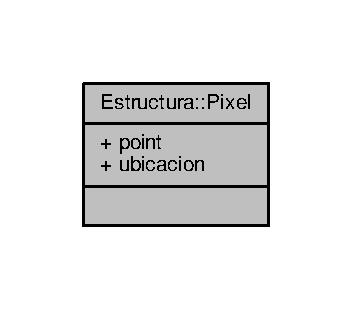
\includegraphics[width=169pt]{structEstructura_1_1Pixel__coll__graph}
\end{center}
\end{figure}
\subsection*{Public Attributes}
\begin{DoxyCompactItemize}
\item 
cv\+::\+Point \hyperlink{structEstructura_1_1Pixel_af5a856559840e7f38fab3147aa576146}{point}
\item 
std\+::vector$<$ int $>$ \hyperlink{structEstructura_1_1Pixel_ac4b5e1358658d9f712933cb20a77d297}{ubicacion}
\end{DoxyCompactItemize}


\subsection{Member Data Documentation}
\index{Estructura\+::\+Pixel@{Estructura\+::\+Pixel}!point@{point}}
\index{point@{point}!Estructura\+::\+Pixel@{Estructura\+::\+Pixel}}
\subsubsection[{\texorpdfstring{point}{point}}]{\setlength{\rightskip}{0pt plus 5cm}cv\+::\+Point Estructura\+::\+Pixel\+::point}\hypertarget{structEstructura_1_1Pixel_af5a856559840e7f38fab3147aa576146}{}\label{structEstructura_1_1Pixel_af5a856559840e7f38fab3147aa576146}


Referenced by Points\+Select\+::generat\+Shoton().

\index{Estructura\+::\+Pixel@{Estructura\+::\+Pixel}!ubicacion@{ubicacion}}
\index{ubicacion@{ubicacion}!Estructura\+::\+Pixel@{Estructura\+::\+Pixel}}
\subsubsection[{\texorpdfstring{ubicacion}{ubicacion}}]{\setlength{\rightskip}{0pt plus 5cm}std\+::vector$<$int$>$ Estructura\+::\+Pixel\+::ubicacion}\hypertarget{structEstructura_1_1Pixel_ac4b5e1358658d9f712933cb20a77d297}{}\label{structEstructura_1_1Pixel_ac4b5e1358658d9f712933cb20a77d297}


Referenced by Points\+Select\+::generat\+Shoton().



The documentation for this struct was generated from the following file\+:\begin{DoxyCompactItemize}
\item 
\hyperlink{Estructura_8h}{Estructura.\+h}\end{DoxyCompactItemize}

\hypertarget{classPointsSelect}{}\section{Points\+Select Class Reference}
\label{classPointsSelect}\index{Points\+Select@{Points\+Select}}


{\ttfamily \#include $<$Points\+Select.\+h$>$}



Collaboration diagram for Points\+Select\+:
\nopagebreak
\begin{figure}[H]
\begin{center}
\leavevmode
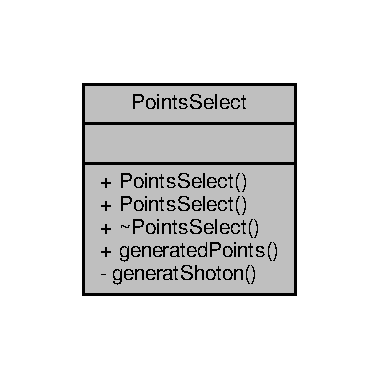
\includegraphics[width=182pt]{classPointsSelect__coll__graph}
\end{center}
\end{figure}
\subsection*{Public Member Functions}
\begin{DoxyCompactItemize}
\item 
\hyperlink{classPointsSelect_add4419dcb7bd7cbe7d8cebbed3b224f5}{Points\+Select} ()
\item 
\hyperlink{classPointsSelect_a78613447513329afc720a9023fff3b03}{Points\+Select} (const \hyperlink{classPointsSelect}{Points\+Select} \&orig)
\item 
virtual \hyperlink{classPointsSelect_a017becb18c1d21eb01f6dc9ffd9461a5}{$\sim$\+Points\+Select} ()
\item 
void \hyperlink{classPointsSelect_a1c487676ff7dc9a8cfd7dbae206a04ae}{generated\+Points} (std\+::string type\+\_\+\+Algorithm, std\+::vector$<$ \hyperlink{structEstructura_1_1Pixel}{Estructura\+::\+Pixel} $>$ \&points, int Num\+Points, int height, int width, int Num\+Tree)
\end{DoxyCompactItemize}
\subsection*{Private Member Functions}
\begin{DoxyCompactItemize}
\item 
void \hyperlink{classPointsSelect_a5b0f15db86a3c16f0e8d6587099d0a9b}{generat\+Shoton} (std\+::vector$<$ \hyperlink{structEstructura_1_1Pixel}{Estructura\+::\+Pixel} $>$ \&points, int Num\+Points, int height, int width, int Num\+Tree)
\end{DoxyCompactItemize}


\subsection{Constructor \& Destructor Documentation}
\index{Points\+Select@{Points\+Select}!Points\+Select@{Points\+Select}}
\index{Points\+Select@{Points\+Select}!Points\+Select@{Points\+Select}}
\subsubsection[{\texorpdfstring{Points\+Select()}{PointsSelect()}}]{\setlength{\rightskip}{0pt plus 5cm}Points\+Select\+::\+Points\+Select (
\begin{DoxyParamCaption}
{}
\end{DoxyParamCaption}
)}\hypertarget{classPointsSelect_add4419dcb7bd7cbe7d8cebbed3b224f5}{}\label{classPointsSelect_add4419dcb7bd7cbe7d8cebbed3b224f5}

\begin{DoxyCode}
16                            \{
17 \}
\end{DoxyCode}
\index{Points\+Select@{Points\+Select}!Points\+Select@{Points\+Select}}
\index{Points\+Select@{Points\+Select}!Points\+Select@{Points\+Select}}
\subsubsection[{\texorpdfstring{Points\+Select(const Points\+Select \&orig)}{PointsSelect(const PointsSelect &orig)}}]{\setlength{\rightskip}{0pt plus 5cm}Points\+Select\+::\+Points\+Select (
\begin{DoxyParamCaption}
\item[{const {\bf Points\+Select} \&}]{orig}
\end{DoxyParamCaption}
)}\hypertarget{classPointsSelect_a78613447513329afc720a9023fff3b03}{}\label{classPointsSelect_a78613447513329afc720a9023fff3b03}

\begin{DoxyCode}
19                                                    \{
20 \}
\end{DoxyCode}
\index{Points\+Select@{Points\+Select}!````~Points\+Select@{$\sim$\+Points\+Select}}
\index{````~Points\+Select@{$\sim$\+Points\+Select}!Points\+Select@{Points\+Select}}
\subsubsection[{\texorpdfstring{$\sim$\+Points\+Select()}{~PointsSelect()}}]{\setlength{\rightskip}{0pt plus 5cm}Points\+Select\+::$\sim$\+Points\+Select (
\begin{DoxyParamCaption}
{}
\end{DoxyParamCaption}
)\hspace{0.3cm}{\ttfamily [virtual]}}\hypertarget{classPointsSelect_a017becb18c1d21eb01f6dc9ffd9461a5}{}\label{classPointsSelect_a017becb18c1d21eb01f6dc9ffd9461a5}

\begin{DoxyCode}
22                             \{
23 \}
\end{DoxyCode}


\subsection{Member Function Documentation}
\index{Points\+Select@{Points\+Select}!generated\+Points@{generated\+Points}}
\index{generated\+Points@{generated\+Points}!Points\+Select@{Points\+Select}}
\subsubsection[{\texorpdfstring{generated\+Points(std\+::string type\+\_\+\+Algorithm, std\+::vector$<$ Estructura\+::\+Pixel $>$ \&points, int Num\+Points, int height, int width, int Num\+Tree)}{generatedPoints(std::string type_Algorithm, std::vector< Estructura::Pixel > &points, int NumPoints, int height, int width, int NumTree)}}]{\setlength{\rightskip}{0pt plus 5cm}void Points\+Select\+::generated\+Points (
\begin{DoxyParamCaption}
\item[{std\+::string}]{type\+\_\+\+Algorithm, }
\item[{std\+::vector$<$ {\bf Estructura\+::\+Pixel} $>$ \&}]{points, }
\item[{int}]{Num\+Points, }
\item[{int}]{height, }
\item[{int}]{width, }
\item[{int}]{Num\+Tree}
\end{DoxyParamCaption}
)}\hypertarget{classPointsSelect_a1c487676ff7dc9a8cfd7dbae206a04ae}{}\label{classPointsSelect_a1c487676ff7dc9a8cfd7dbae206a04ae}


References generat\+Shoton().



Referenced by Image\+::generated\+Structure\+Shotton().


\begin{DoxyCode}
25                                                                                                            
                                            \{
26     
27     std::vector<Estructura::Pixel> temporal;
28     \textcolor{keywordflow}{if}(type\_Algorithm.compare(0,7,\textcolor{stringliteral}{"shotton"}) == 0)\{
29         \hyperlink{classPointsSelect_a5b0f15db86a3c16f0e8d6587099d0a9b}{generatShoton}(temporal, NumPoints, height, width, NumTree);
30         
31     \}
32     points = temporal;
33 \}
\end{DoxyCode}
\index{Points\+Select@{Points\+Select}!generat\+Shoton@{generat\+Shoton}}
\index{generat\+Shoton@{generat\+Shoton}!Points\+Select@{Points\+Select}}
\subsubsection[{\texorpdfstring{generat\+Shoton(std\+::vector$<$ Estructura\+::\+Pixel $>$ \&points, int Num\+Points, int height, int width, int Num\+Tree)}{generatShoton(std::vector< Estructura::Pixel > &points, int NumPoints, int height, int width, int NumTree)}}]{\setlength{\rightskip}{0pt plus 5cm}void Points\+Select\+::generat\+Shoton (
\begin{DoxyParamCaption}
\item[{std\+::vector$<$ {\bf Estructura\+::\+Pixel} $>$ \&}]{points, }
\item[{int}]{Num\+Points, }
\item[{int}]{height, }
\item[{int}]{width, }
\item[{int}]{Num\+Tree}
\end{DoxyParamCaption}
)\hspace{0.3cm}{\ttfamily [private]}}\hypertarget{classPointsSelect_a5b0f15db86a3c16f0e8d6587099d0a9b}{}\label{classPointsSelect_a5b0f15db86a3c16f0e8d6587099d0a9b}


References Estructura\+::\+Pixel\+::point, and Estructura\+::\+Pixel\+::ubicacion.



Referenced by generated\+Points().


\begin{DoxyCode}
35                                                                                                            
                \{
36     
37     
38     std::vector<int> start (NumTree,0);
39     \hyperlink{structEstructura_1_1Pixel}{Estructura::Pixel} pixelTemp;
40     
41     \textcolor{keywordflow}{for} (\textcolor{keywordtype}{int} i = 0; i < NumPoints; i++) \{
42         pixelTemp.\hyperlink{structEstructura_1_1Pixel_af5a856559840e7f38fab3147aa576146}{point} = cv::Point((rand() % (height - 0)),((rand() % (width - 0))));
43         pixelTemp.\hyperlink{structEstructura_1_1Pixel_ac4b5e1358658d9f712933cb20a77d297}{ubicacion} = start;
44         points.push\_back(pixelTemp);
45     \}
46 \}
\end{DoxyCode}


The documentation for this class was generated from the following files\+:\begin{DoxyCompactItemize}
\item 
\hyperlink{PointsSelect_8h}{Points\+Select.\+h}\item 
\hyperlink{PointsSelect_8cpp}{Points\+Select.\+cpp}\end{DoxyCompactItemize}

\hypertarget{structQueueTask_1_1Queue}{}\section{Queue\+Task\+:\+:Queue Struct Reference}
\label{structQueueTask_1_1Queue}\index{Queue\+Task\+::\+Queue@{Queue\+Task\+::\+Queue}}


{\ttfamily \#include $<$Queue\+Task.\+h$>$}



Collaboration diagram for Queue\+Task\+:\+:Queue\+:
\nopagebreak
\begin{figure}[H]
\begin{center}
\leavevmode
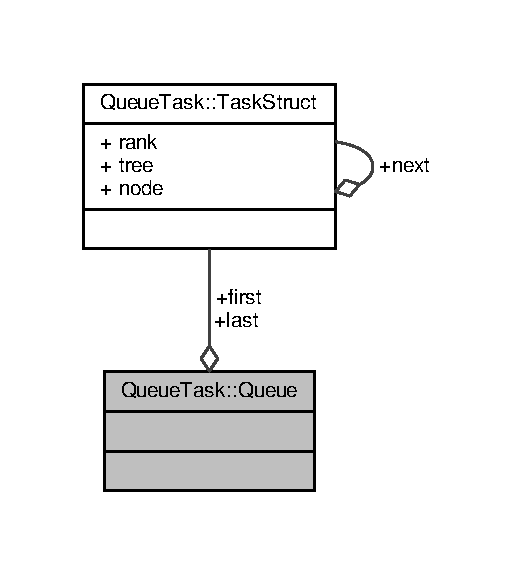
\includegraphics[width=247pt]{structQueueTask_1_1Queue__coll__graph}
\end{center}
\end{figure}
\subsection*{Public Attributes}
\begin{DoxyCompactItemize}
\item 
\hyperlink{structQueueTask_1_1TaskStruct}{Task\+Struct} $\ast$ \hyperlink{structQueueTask_1_1Queue_aefe07ecf93c1276d1436e57656799a41}{first}
\item 
\hyperlink{structQueueTask_1_1TaskStruct}{Task\+Struct} $\ast$ \hyperlink{structQueueTask_1_1Queue_a886474ef2f7fab2904fb36edf4802350}{last}
\end{DoxyCompactItemize}


\subsection{Member Data Documentation}
\index{Queue\+Task\+::\+Queue@{Queue\+Task\+::\+Queue}!first@{first}}
\index{first@{first}!Queue\+Task\+::\+Queue@{Queue\+Task\+::\+Queue}}
\subsubsection[{\texorpdfstring{first}{first}}]{\setlength{\rightskip}{0pt plus 5cm}{\bf Task\+Struct}$\ast$ Queue\+Task\+::\+Queue\+::first}\hypertarget{structQueueTask_1_1Queue_aefe07ecf93c1276d1436e57656799a41}{}\label{structQueueTask_1_1Queue_aefe07ecf93c1276d1436e57656799a41}


Referenced by Queue\+Task\+::add\+Queue(), Queue\+Task\+::display\+Queue\+Tasks(), Queue\+Task\+::get\+Number\+Elements(), Queue\+Task\+::is\+Empty(), Queue\+Task\+::pop(), and Queue\+Task\+::sort\+Priority().

\index{Queue\+Task\+::\+Queue@{Queue\+Task\+::\+Queue}!last@{last}}
\index{last@{last}!Queue\+Task\+::\+Queue@{Queue\+Task\+::\+Queue}}
\subsubsection[{\texorpdfstring{last}{last}}]{\setlength{\rightskip}{0pt plus 5cm}{\bf Task\+Struct}$\ast$ Queue\+Task\+::\+Queue\+::last}\hypertarget{structQueueTask_1_1Queue_a886474ef2f7fab2904fb36edf4802350}{}\label{structQueueTask_1_1Queue_a886474ef2f7fab2904fb36edf4802350}


Referenced by Queue\+Task\+::add\+Queue().



The documentation for this struct was generated from the following file\+:\begin{DoxyCompactItemize}
\item 
\hyperlink{QueueTask_8h}{Queue\+Task.\+h}\end{DoxyCompactItemize}

\hypertarget{classQueueTask}{}\section{Queue\+Task Class Reference}
\label{classQueueTask}\index{Queue\+Task@{Queue\+Task}}


{\ttfamily \#include $<$Queue\+Task.\+h$>$}



Collaboration diagram for Queue\+Task\+:
\nopagebreak
\begin{figure}[H]
\begin{center}
\leavevmode
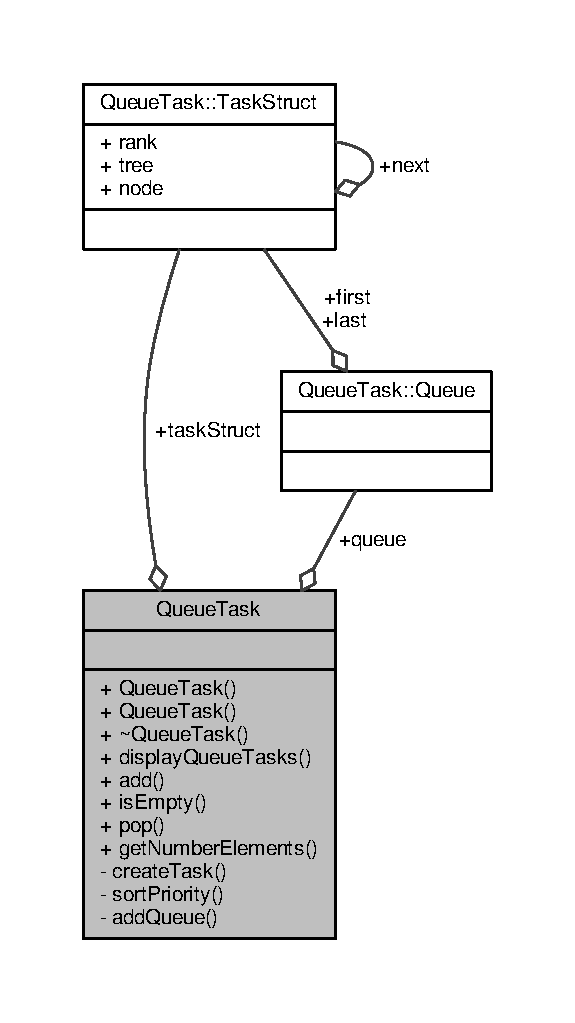
\includegraphics[width=276pt]{classQueueTask__coll__graph}
\end{center}
\end{figure}
\subsection*{Classes}
\begin{DoxyCompactItemize}
\item 
struct \hyperlink{structQueueTask_1_1Queue}{Queue}
\item 
struct \hyperlink{structQueueTask_1_1TaskStruct}{Task\+Struct}
\end{DoxyCompactItemize}
\subsection*{Public Member Functions}
\begin{DoxyCompactItemize}
\item 
\hyperlink{classQueueTask_aa9b9477fcb1242fc8b357b3f7416752c}{Queue\+Task} ()
\item 
\hyperlink{classQueueTask_a326a20304f894ef5cec9e0a275496ce7}{Queue\+Task} (const \hyperlink{classQueueTask}{Queue\+Task} \&orig)
\item 
virtual \hyperlink{classQueueTask_a9ed7eebd0806d5de8b977c7e8d40dee7}{$\sim$\+Queue\+Task} ()
\item 
void \hyperlink{classQueueTask_a37f73c5339ef2c9d1266430b8f741999}{display\+Queue\+Tasks} (struct \hyperlink{structQueueTask_1_1Queue}{Queue} tasks)
\item 
void \hyperlink{classQueueTask_a5cb3f2197e8ca06187ca3c3afcc95e2b}{add} (struct \hyperlink{structQueueTask_1_1Queue}{Queue} \&tasks, int rank, int tree, int node)
\item 
void \hyperlink{classQueueTask_a32187b71e7fc4b94c029bfa3183440a6}{is\+Empty} (struct \hyperlink{structQueueTask_1_1Queue}{Queue} tasks, bool \&empty)
\item 
void \hyperlink{classQueueTask_a95870b68177d6b6cdd36cec23f80811c}{pop} (struct \hyperlink{structQueueTask_1_1Queue}{Queue} \&tasks, struct \hyperlink{structQueueTask_1_1TaskStruct}{Task\+Struct} \&task)
\item 
void \hyperlink{classQueueTask_a798f3e860e39a4c9ce4aaa3bca64b63f}{get\+Number\+Elements} (struct \hyperlink{structQueueTask_1_1Queue}{Queue} \&tasks, int \&number\+Elements)
\end{DoxyCompactItemize}
\subsection*{Public Attributes}
\begin{DoxyCompactItemize}
\item 
struct \hyperlink{structQueueTask_1_1TaskStruct}{Queue\+Task\+::\+Task\+Struct} \hyperlink{classQueueTask_aa62b59622aa85704f0adedfd9a56ece2}{task\+Struct}
\item 
struct \hyperlink{structQueueTask_1_1Queue}{Queue\+Task\+::\+Queue} \hyperlink{classQueueTask_a5dcac92fbafbc338f87bcf5f2b5b2919}{queue}
\end{DoxyCompactItemize}
\subsection*{Private Member Functions}
\begin{DoxyCompactItemize}
\item 
struct \hyperlink{structQueueTask_1_1TaskStruct}{Task\+Struct} $\ast$ \hyperlink{classQueueTask_a84998ffe350640959aa186a9f283320c}{create\+Task} (int rank, int tree, int node)
\item 
void \hyperlink{classQueueTask_a4c2692a068505a40559bf101a0ad64cb}{sort\+Priority} (struct \hyperlink{structQueueTask_1_1Queue}{Queue} \&tasks)
\item 
void \hyperlink{classQueueTask_ad32628f249dc718ec9342d7e043371ee}{add\+Queue} (struct \hyperlink{structQueueTask_1_1Queue}{Queue} \&tasks, int rank, int tree, int node)
\end{DoxyCompactItemize}


\subsection{Constructor \& Destructor Documentation}
\index{Queue\+Task@{Queue\+Task}!Queue\+Task@{Queue\+Task}}
\index{Queue\+Task@{Queue\+Task}!Queue\+Task@{Queue\+Task}}
\subsubsection[{\texorpdfstring{Queue\+Task()}{QueueTask()}}]{\setlength{\rightskip}{0pt plus 5cm}Queue\+Task\+::\+Queue\+Task (
\begin{DoxyParamCaption}
{}
\end{DoxyParamCaption}
)}\hypertarget{classQueueTask_aa9b9477fcb1242fc8b357b3f7416752c}{}\label{classQueueTask_aa9b9477fcb1242fc8b357b3f7416752c}

\begin{DoxyCode}
17                      \{
18 
19 \}
\end{DoxyCode}
\index{Queue\+Task@{Queue\+Task}!Queue\+Task@{Queue\+Task}}
\index{Queue\+Task@{Queue\+Task}!Queue\+Task@{Queue\+Task}}
\subsubsection[{\texorpdfstring{Queue\+Task(const Queue\+Task \&orig)}{QueueTask(const QueueTask &orig)}}]{\setlength{\rightskip}{0pt plus 5cm}Queue\+Task\+::\+Queue\+Task (
\begin{DoxyParamCaption}
\item[{const {\bf Queue\+Task} \&}]{orig}
\end{DoxyParamCaption}
)}\hypertarget{classQueueTask_a326a20304f894ef5cec9e0a275496ce7}{}\label{classQueueTask_a326a20304f894ef5cec9e0a275496ce7}

\begin{DoxyCode}
21                                           \{
22 \}
\end{DoxyCode}
\index{Queue\+Task@{Queue\+Task}!````~Queue\+Task@{$\sim$\+Queue\+Task}}
\index{````~Queue\+Task@{$\sim$\+Queue\+Task}!Queue\+Task@{Queue\+Task}}
\subsubsection[{\texorpdfstring{$\sim$\+Queue\+Task()}{~QueueTask()}}]{\setlength{\rightskip}{0pt plus 5cm}Queue\+Task\+::$\sim$\+Queue\+Task (
\begin{DoxyParamCaption}
{}
\end{DoxyParamCaption}
)\hspace{0.3cm}{\ttfamily [virtual]}}\hypertarget{classQueueTask_a9ed7eebd0806d5de8b977c7e8d40dee7}{}\label{classQueueTask_a9ed7eebd0806d5de8b977c7e8d40dee7}

\begin{DoxyCode}
24                       \{
25 \}
\end{DoxyCode}


\subsection{Member Function Documentation}
\index{Queue\+Task@{Queue\+Task}!add@{add}}
\index{add@{add}!Queue\+Task@{Queue\+Task}}
\subsubsection[{\texorpdfstring{add(struct Queue \&tasks, int rank, int tree, int node)}{add(struct Queue &tasks, int rank, int tree, int node)}}]{\setlength{\rightskip}{0pt plus 5cm}void Queue\+Task\+::add (
\begin{DoxyParamCaption}
\item[{struct {\bf Queue} \&}]{tasks, }
\item[{int}]{rank, }
\item[{int}]{tree, }
\item[{int}]{node}
\end{DoxyParamCaption}
)}\hypertarget{classQueueTask_a5cb3f2197e8ca06187ca3c3afcc95e2b}{}\label{classQueueTask_a5cb3f2197e8ca06187ca3c3afcc95e2b}


References add\+Queue(), and sort\+Priority().


\begin{DoxyCode}
104                                                               \{
105     \hyperlink{classQueueTask_ad32628f249dc718ec9342d7e043371ee}{addQueue}(tasks, rank, tree, node);
106     \hyperlink{classQueueTask_a4c2692a068505a40559bf101a0ad64cb}{sortPriority}(tasks);
107 \}
\end{DoxyCode}
\index{Queue\+Task@{Queue\+Task}!add\+Queue@{add\+Queue}}
\index{add\+Queue@{add\+Queue}!Queue\+Task@{Queue\+Task}}
\subsubsection[{\texorpdfstring{add\+Queue(struct Queue \&tasks, int rank, int tree, int node)}{addQueue(struct Queue &tasks, int rank, int tree, int node)}}]{\setlength{\rightskip}{0pt plus 5cm}void Queue\+Task\+::add\+Queue (
\begin{DoxyParamCaption}
\item[{struct {\bf Queue} \&}]{tasks, }
\item[{int}]{rank, }
\item[{int}]{tree, }
\item[{int}]{node}
\end{DoxyParamCaption}
)\hspace{0.3cm}{\ttfamily [private]}}\hypertarget{classQueueTask_ad32628f249dc718ec9342d7e043371ee}{}\label{classQueueTask_ad32628f249dc718ec9342d7e043371ee}


References create\+Task(), Queue\+Task\+::\+Queue\+::first, Queue\+Task\+::\+Queue\+::last, and Queue\+Task\+::\+Task\+Struct\+::next.



Referenced by add().


\begin{DoxyCode}
43                                                                    \{
44     \textcolor{keyword}{struct }\hyperlink{structQueueTask_1_1TaskStruct}{QueueTask::TaskStruct} *aux = \hyperlink{classQueueTask_a84998ffe350640959aa186a9f283320c}{createTask}(
      \hyperlink{structQueueTask_1_1TaskStruct_af9877fb064cb899ac88ffef431d98f47}{rank}, \hyperlink{structQueueTask_1_1TaskStruct_a6b1c9ba8e5b30acfa78e61c95c7cb897}{tree}, \hyperlink{structQueueTask_1_1TaskStruct_a22eb8e22f500809266c4983897b9af7f}{node});
45     aux->\hyperlink{structQueueTask_1_1TaskStruct_aff77873a32e938c956c84deb01f98e65}{next} = 0;
46 
47     \textcolor{keywordflow}{if} (tasks.first == NULL) \{
48         tasks.first = aux;
49     \} \textcolor{keywordflow}{else} \{
50         tasks.last->\hyperlink{structQueueTask_1_1TaskStruct_aff77873a32e938c956c84deb01f98e65}{next} = aux;
51     \}
52 
53     tasks.last = aux;
54 \}
\end{DoxyCode}
\index{Queue\+Task@{Queue\+Task}!create\+Task@{create\+Task}}
\index{create\+Task@{create\+Task}!Queue\+Task@{Queue\+Task}}
\subsubsection[{\texorpdfstring{create\+Task(int rank, int tree, int node)}{createTask(int rank, int tree, int node)}}]{\setlength{\rightskip}{0pt plus 5cm}struct {\bf Queue\+Task\+::\+Task\+Struct} $\ast$ Queue\+Task\+::create\+Task (
\begin{DoxyParamCaption}
\item[{int}]{rank, }
\item[{int}]{tree, }
\item[{int}]{node}
\end{DoxyParamCaption}
)\hspace{0.3cm}{\ttfamily [private]}}\hypertarget{classQueueTask_a84998ffe350640959aa186a9f283320c}{}\label{classQueueTask_a84998ffe350640959aa186a9f283320c}


References Queue\+Task\+::\+Task\+Struct\+::node, Queue\+Task\+::\+Task\+Struct\+::rank, and Queue\+Task\+::\+Task\+Struct\+::tree.



Referenced by add\+Queue().


\begin{DoxyCode}
35                                                                               \{
36     \textcolor{keyword}{struct }\hyperlink{structQueueTask_1_1TaskStruct}{QueueTask::TaskStruct} *newTask = \textcolor{keyword}{new} (\textcolor{keyword}{struct }
      \hyperlink{structQueueTask_1_1TaskStruct}{QueueTask::TaskStruct});
37     newTask->\hyperlink{structQueueTask_1_1TaskStruct_af9877fb064cb899ac88ffef431d98f47}{rank} = \hyperlink{structQueueTask_1_1TaskStruct_af9877fb064cb899ac88ffef431d98f47}{rank};
38     newTask->\hyperlink{structQueueTask_1_1TaskStruct_a22eb8e22f500809266c4983897b9af7f}{node} = \hyperlink{structQueueTask_1_1TaskStruct_a22eb8e22f500809266c4983897b9af7f}{node};
39     newTask->\hyperlink{structQueueTask_1_1TaskStruct_a6b1c9ba8e5b30acfa78e61c95c7cb897}{tree} = \hyperlink{structQueueTask_1_1TaskStruct_a6b1c9ba8e5b30acfa78e61c95c7cb897}{tree};
40     \textcolor{keywordflow}{return} newTask;
41 \}
\end{DoxyCode}
\index{Queue\+Task@{Queue\+Task}!display\+Queue\+Tasks@{display\+Queue\+Tasks}}
\index{display\+Queue\+Tasks@{display\+Queue\+Tasks}!Queue\+Task@{Queue\+Task}}
\subsubsection[{\texorpdfstring{display\+Queue\+Tasks(struct Queue tasks)}{displayQueueTasks(struct Queue tasks)}}]{\setlength{\rightskip}{0pt plus 5cm}void Queue\+Task\+::display\+Queue\+Tasks (
\begin{DoxyParamCaption}
\item[{struct {\bf Queue}}]{tasks}
\end{DoxyParamCaption}
)}\hypertarget{classQueueTask_a37f73c5339ef2c9d1266430b8f741999}{}\label{classQueueTask_a37f73c5339ef2c9d1266430b8f741999}


References Queue\+Task\+::\+Queue\+::first, Queue\+Task\+::\+Task\+Struct\+::next, Queue\+Task\+::\+Task\+Struct\+::node, Queue\+Task\+::\+Task\+Struct\+::rank, and Queue\+Task\+::\+Task\+Struct\+::tree.


\begin{DoxyCode}
56                                              \{
57     \textcolor{keyword}{struct }\hyperlink{structQueueTask_1_1TaskStruct}{QueueTask::TaskStruct} *aux;
58 
59     aux = tasks.first;
60     std::cout << \textcolor{stringliteral}{"Las tareas son: "} << \textcolor{stringliteral}{"\(\backslash\)n"};
61     std::cout << \textcolor{stringliteral}{"****************"} << \textcolor{stringliteral}{"\(\backslash\)n"};
62 
63     \textcolor{keywordflow}{while} (aux != NULL) \{
64         std::cout << \textcolor{stringliteral}{"Tree:  "} << aux->\hyperlink{structQueueTask_1_1TaskStruct_a6b1c9ba8e5b30acfa78e61c95c7cb897}{tree} << \textcolor{stringliteral}{" Node:   "} << aux->\hyperlink{structQueueTask_1_1TaskStruct_a22eb8e22f500809266c4983897b9af7f}{node} << \textcolor{stringliteral}{" Rank:   "} << aux->
      \hyperlink{structQueueTask_1_1TaskStruct_af9877fb064cb899ac88ffef431d98f47}{rank} << std::endl;
65         aux = aux->\hyperlink{structQueueTask_1_1TaskStruct_aff77873a32e938c956c84deb01f98e65}{next};
66     \}
67 \}
\end{DoxyCode}
\index{Queue\+Task@{Queue\+Task}!get\+Number\+Elements@{get\+Number\+Elements}}
\index{get\+Number\+Elements@{get\+Number\+Elements}!Queue\+Task@{Queue\+Task}}
\subsubsection[{\texorpdfstring{get\+Number\+Elements(struct Queue \&tasks, int \&number\+Elements)}{getNumberElements(struct Queue &tasks, int &numberElements)}}]{\setlength{\rightskip}{0pt plus 5cm}void Queue\+Task\+::get\+Number\+Elements (
\begin{DoxyParamCaption}
\item[{struct {\bf Queue} \&}]{tasks, }
\item[{int \&}]{number\+Elements}
\end{DoxyParamCaption}
)}\hypertarget{classQueueTask_a798f3e860e39a4c9ce4aaa3bca64b63f}{}\label{classQueueTask_a798f3e860e39a4c9ce4aaa3bca64b63f}


References Queue\+Task\+::\+Queue\+::first, and Queue\+Task\+::\+Task\+Struct\+::next.


\begin{DoxyCode}
133                                                                   \{
134     \textcolor{keyword}{struct }\hyperlink{structQueueTask_1_1TaskStruct}{QueueTask::TaskStruct} *aux;
135 
136     aux = tasks.first;
137     numberElements = 0;
138     \textcolor{keywordflow}{while} (aux != NULL) \{
139         aux = aux->\hyperlink{structQueueTask_1_1TaskStruct_aff77873a32e938c956c84deb01f98e65}{next};
140         numberElements +=1;
141     \}
142 \}\end{DoxyCode}
\index{Queue\+Task@{Queue\+Task}!is\+Empty@{is\+Empty}}
\index{is\+Empty@{is\+Empty}!Queue\+Task@{Queue\+Task}}
\subsubsection[{\texorpdfstring{is\+Empty(struct Queue tasks, bool \&empty)}{isEmpty(struct Queue tasks, bool &empty)}}]{\setlength{\rightskip}{0pt plus 5cm}void Queue\+Task\+::is\+Empty (
\begin{DoxyParamCaption}
\item[{struct {\bf Queue}}]{tasks, }
\item[{bool \&}]{empty}
\end{DoxyParamCaption}
)}\hypertarget{classQueueTask_a32187b71e7fc4b94c029bfa3183440a6}{}\label{classQueueTask_a32187b71e7fc4b94c029bfa3183440a6}


References Queue\+Task\+::\+Queue\+::first.


\begin{DoxyCode}
109                                                 \{
110 
111     \textcolor{keywordflow}{if} (tasks.first == NULL) \{
112         empty = \textcolor{keyword}{true};
113     \} \textcolor{keywordflow}{else} \{
114         empty = \textcolor{keyword}{false};
115     \}
116 \}
\end{DoxyCode}
\index{Queue\+Task@{Queue\+Task}!pop@{pop}}
\index{pop@{pop}!Queue\+Task@{Queue\+Task}}
\subsubsection[{\texorpdfstring{pop(struct Queue \&tasks, struct Task\+Struct \&task)}{pop(struct Queue &tasks, struct TaskStruct &task)}}]{\setlength{\rightskip}{0pt plus 5cm}void Queue\+Task\+::pop (
\begin{DoxyParamCaption}
\item[{struct {\bf Queue} \&}]{tasks, }
\item[{struct {\bf Task\+Struct} \&}]{task}
\end{DoxyParamCaption}
)}\hypertarget{classQueueTask_a95870b68177d6b6cdd36cec23f80811c}{}\label{classQueueTask_a95870b68177d6b6cdd36cec23f80811c}


References Queue\+Task\+::\+Queue\+::first, and Queue\+Task\+::\+Task\+Struct\+::next.


\begin{DoxyCode}
118                                                                 \{
119     \textcolor{keyword}{struct }\hyperlink{structQueueTask_1_1TaskStruct}{QueueTask::TaskStruct} *aux;
120     aux = tasks.first;
121 
122     \textcolor{keywordflow}{if} (tasks.first != NULL) \{
123         tasks.first = aux->\hyperlink{structQueueTask_1_1TaskStruct_aff77873a32e938c956c84deb01f98e65}{next};
124         aux->\hyperlink{structQueueTask_1_1TaskStruct_aff77873a32e938c956c84deb01f98e65}{next} = NULL;
125 
126     \} \textcolor{keywordflow}{else} \{
127         std::cout << \textcolor{stringliteral}{"La lista esta vacia"} << \textcolor{stringliteral}{"\(\backslash\)n"};
128     \}
129     task = *aux;
130     \textcolor{keyword}{delete} aux;
131 \}
\end{DoxyCode}
\index{Queue\+Task@{Queue\+Task}!sort\+Priority@{sort\+Priority}}
\index{sort\+Priority@{sort\+Priority}!Queue\+Task@{Queue\+Task}}
\subsubsection[{\texorpdfstring{sort\+Priority(struct Queue \&tasks)}{sortPriority(struct Queue &tasks)}}]{\setlength{\rightskip}{0pt plus 5cm}void Queue\+Task\+::sort\+Priority (
\begin{DoxyParamCaption}
\item[{struct {\bf Queue} \&}]{tasks}
\end{DoxyParamCaption}
)\hspace{0.3cm}{\ttfamily [private]}}\hypertarget{classQueueTask_a4c2692a068505a40559bf101a0ad64cb}{}\label{classQueueTask_a4c2692a068505a40559bf101a0ad64cb}


References Queue\+Task\+::\+Queue\+::first, Queue\+Task\+::\+Task\+Struct\+::next, Queue\+Task\+::\+Task\+Struct\+::node, Queue\+Task\+::\+Task\+Struct\+::rank, and Queue\+Task\+::\+Task\+Struct\+::tree.



Referenced by add().


\begin{DoxyCode}
69                                          \{
70     \textcolor{keyword}{struct }\hyperlink{structQueueTask_1_1TaskStruct}{QueueTask::TaskStruct} *aux1, *aux2;
71     \textcolor{keywordtype}{int} treeAux;
72     \textcolor{keywordtype}{int} nodeAux;
73     \textcolor{keywordtype}{int} rankAux;
74 
75     aux1 = tasks.first;
76 
77     \textcolor{keywordflow}{while} (aux1->\hyperlink{structQueueTask_1_1TaskStruct_aff77873a32e938c956c84deb01f98e65}{next} != NULL) \{
78         aux2 = aux1->\hyperlink{structQueueTask_1_1TaskStruct_aff77873a32e938c956c84deb01f98e65}{next};
79 
80         \textcolor{keywordflow}{while} (aux2 != NULL) \{
81             \textcolor{keywordflow}{if} (aux1->\hyperlink{structQueueTask_1_1TaskStruct_a6b1c9ba8e5b30acfa78e61c95c7cb897}{tree} >= aux2->\hyperlink{structQueueTask_1_1TaskStruct_a6b1c9ba8e5b30acfa78e61c95c7cb897}{tree}) \{
82 
83                 \textcolor{keywordflow}{if} (aux1->\hyperlink{structQueueTask_1_1TaskStruct_a22eb8e22f500809266c4983897b9af7f}{node} > aux2->\hyperlink{structQueueTask_1_1TaskStruct_a22eb8e22f500809266c4983897b9af7f}{node}) \{
84                     treeAux = aux1->\hyperlink{structQueueTask_1_1TaskStruct_a6b1c9ba8e5b30acfa78e61c95c7cb897}{tree};
85                     nodeAux = aux1->\hyperlink{structQueueTask_1_1TaskStruct_a22eb8e22f500809266c4983897b9af7f}{node};
86                     rankAux = aux1->\hyperlink{structQueueTask_1_1TaskStruct_af9877fb064cb899ac88ffef431d98f47}{rank};
87 
88                     aux1->\hyperlink{structQueueTask_1_1TaskStruct_a6b1c9ba8e5b30acfa78e61c95c7cb897}{tree} = aux2->\hyperlink{structQueueTask_1_1TaskStruct_a6b1c9ba8e5b30acfa78e61c95c7cb897}{tree};
89                     aux1->\hyperlink{structQueueTask_1_1TaskStruct_a22eb8e22f500809266c4983897b9af7f}{node} = aux2->\hyperlink{structQueueTask_1_1TaskStruct_a22eb8e22f500809266c4983897b9af7f}{node};
90                     aux1->\hyperlink{structQueueTask_1_1TaskStruct_af9877fb064cb899ac88ffef431d98f47}{rank} = aux2->\hyperlink{structQueueTask_1_1TaskStruct_af9877fb064cb899ac88ffef431d98f47}{rank};
91 
92                     aux2->\hyperlink{structQueueTask_1_1TaskStruct_a6b1c9ba8e5b30acfa78e61c95c7cb897}{tree} = treeAux;
93                     aux2->\hyperlink{structQueueTask_1_1TaskStruct_a22eb8e22f500809266c4983897b9af7f}{node} = nodeAux;
94                     aux2->\hyperlink{structQueueTask_1_1TaskStruct_af9877fb064cb899ac88ffef431d98f47}{rank} = rankAux;
95                 \}
96             \}
97 
98             aux2 = aux2->\hyperlink{structQueueTask_1_1TaskStruct_aff77873a32e938c956c84deb01f98e65}{next};
99         \}
100         aux1 = aux1->\hyperlink{structQueueTask_1_1TaskStruct_aff77873a32e938c956c84deb01f98e65}{next};
101     \}
102 \}
\end{DoxyCode}


\subsection{Member Data Documentation}
\index{Queue\+Task@{Queue\+Task}!queue@{queue}}
\index{queue@{queue}!Queue\+Task@{Queue\+Task}}
\subsubsection[{\texorpdfstring{queue}{queue}}]{\setlength{\rightskip}{0pt plus 5cm}struct {\bf Queue\+Task\+::\+Queue}  Queue\+Task\+::queue}\hypertarget{classQueueTask_a5dcac92fbafbc338f87bcf5f2b5b2919}{}\label{classQueueTask_a5dcac92fbafbc338f87bcf5f2b5b2919}
\index{Queue\+Task@{Queue\+Task}!task\+Struct@{task\+Struct}}
\index{task\+Struct@{task\+Struct}!Queue\+Task@{Queue\+Task}}
\subsubsection[{\texorpdfstring{task\+Struct}{taskStruct}}]{\setlength{\rightskip}{0pt plus 5cm}struct {\bf Queue\+Task\+::\+Task\+Struct}  Queue\+Task\+::task\+Struct}\hypertarget{classQueueTask_aa62b59622aa85704f0adedfd9a56ece2}{}\label{classQueueTask_aa62b59622aa85704f0adedfd9a56ece2}


The documentation for this class was generated from the following files\+:\begin{DoxyCompactItemize}
\item 
\hyperlink{QueueTask_8h}{Queue\+Task.\+h}\item 
\hyperlink{QueueTask_8cpp}{Queue\+Task.\+cpp}\end{DoxyCompactItemize}

\hypertarget{classQueueThread}{}\section{Queue\+Thread Class Reference}
\label{classQueueThread}\index{Queue\+Thread@{Queue\+Thread}}


{\ttfamily \#include $<$Queue\+Thread.\+h$>$}



Collaboration diagram for Queue\+Thread\+:
\nopagebreak
\begin{figure}[H]
\begin{center}
\leavevmode
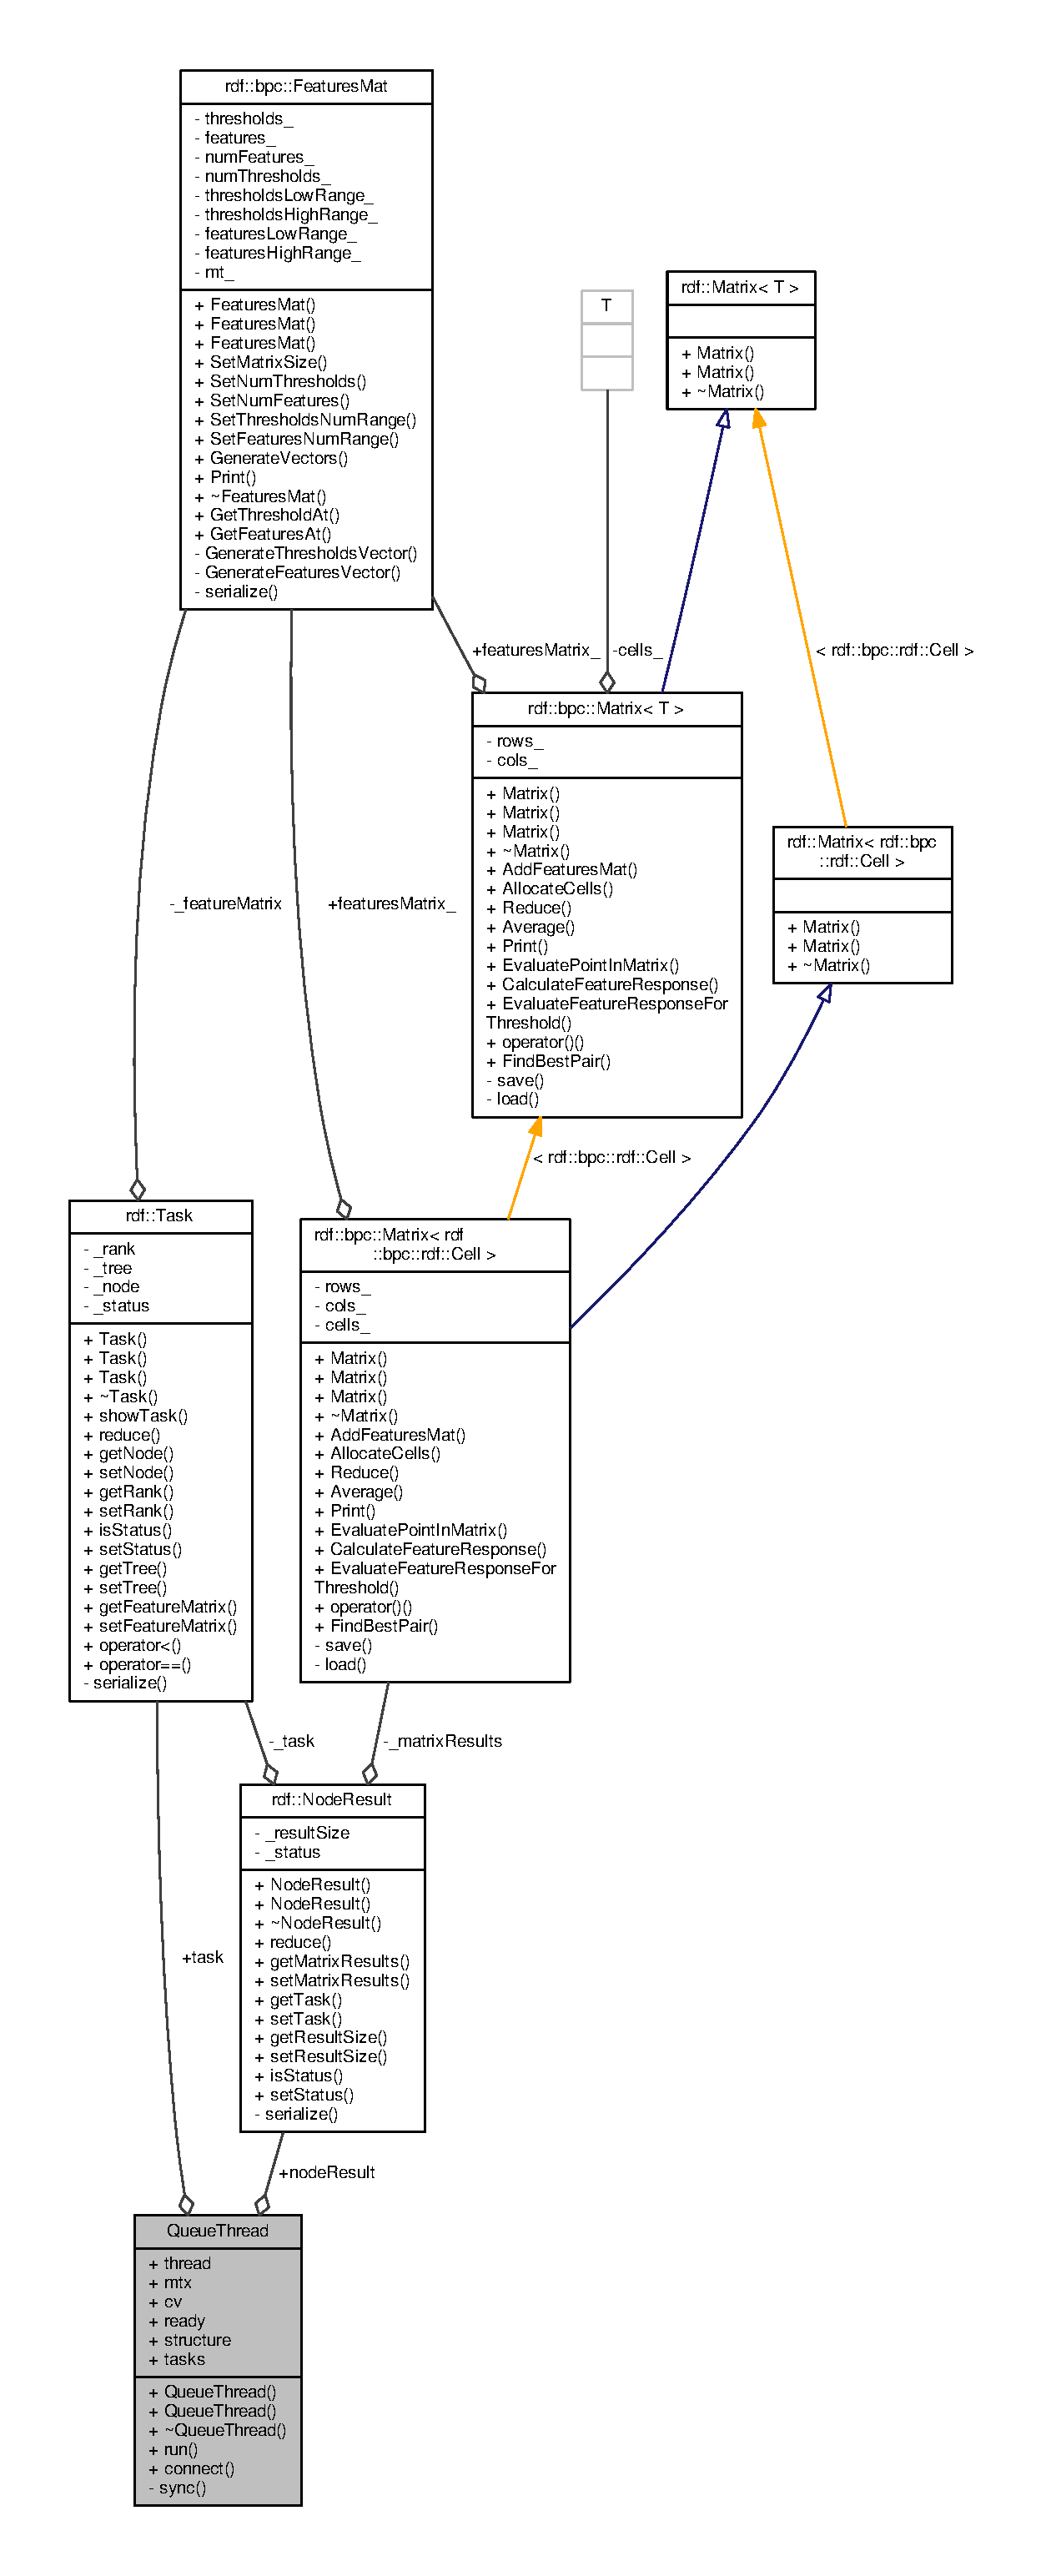
\includegraphics[height=550pt]{classQueueThread__coll__graph}
\end{center}
\end{figure}
\subsection*{Public Member Functions}
\begin{DoxyCompactItemize}
\item 
\hyperlink{classQueueThread_a67e91d4fedd650255e9389c50b4e6749}{Queue\+Thread} ()
\item 
\hyperlink{classQueueThread_a4a48439ac971b82fa1dd1b63138a4d2b}{Queue\+Thread} (const \hyperlink{classQueueThread}{Queue\+Thread} \&orig)
\item 
virtual \hyperlink{classQueueThread_aeca7000eb51c2f4d2ec33352c8e08ec3}{$\sim$\+Queue\+Thread} ()
\item 
void \hyperlink{classQueueThread_a73db1449c750aab9c973592a69f12e85}{run} ()
\item 
void \hyperlink{classQueueThread_a873d5d9edf446f44467518c8fbde1800}{connect} (std\+::vector$<$ \hyperlink{structEstructura_1_1Node}{Estructura\+::\+Node} $>$ \hyperlink{classQueueThread_ab591bae3315c80df7fa723db66e763fa}{structure}, \hyperlink{classrdf_1_1Task}{rdf\+::\+Task} \hyperlink{classQueueThread_a4cf069642e3f67ff759a2163fa2ef3ce}{task}, std\+::priority\+\_\+queue$<$ \hyperlink{classrdf_1_1Task}{rdf\+::\+Task} $>$ \hyperlink{classQueueThread_a8e8f59dccfcb4a213db1b42aec0e4f4d}{tasks}, \hyperlink{classrdf_1_1NodeResult}{rdf\+::\+Node\+Result} \&\hyperlink{classQueueThread_aa775f99b02ff36d5336212ae53bd12b4}{node\+Result})
\end{DoxyCompactItemize}
\subsection*{Public Attributes}
\begin{DoxyCompactItemize}
\item 
std\+::thread \hyperlink{classQueueThread_a91bdd16de58d62287968b80f68620033}{thread}
\item 
std\+::mutex \hyperlink{classQueueThread_a7bf4df2e118ced2e8fbbac3af8992d79}{mtx}
\item 
std\+::condition\+\_\+variable \hyperlink{classQueueThread_a51fdcc17ea346cf6bbc51467d49e9696}{cv}
\item 
bool \hyperlink{classQueueThread_a26f11295bff95a8a44bb75a58168d611}{ready} = false
\item 
std\+::vector$<$ \hyperlink{structEstructura_1_1Node}{Estructura\+::\+Node} $>$ \hyperlink{classQueueThread_ab591bae3315c80df7fa723db66e763fa}{structure}
\item 
\hyperlink{classrdf_1_1Task}{rdf\+::\+Task} \hyperlink{classQueueThread_a4cf069642e3f67ff759a2163fa2ef3ce}{task}
\item 
std\+::priority\+\_\+queue$<$ \hyperlink{classrdf_1_1Task}{rdf\+::\+Task} $>$ \hyperlink{classQueueThread_a8e8f59dccfcb4a213db1b42aec0e4f4d}{tasks}
\item 
\hyperlink{classrdf_1_1NodeResult}{rdf\+::\+Node\+Result} \hyperlink{classQueueThread_aa775f99b02ff36d5336212ae53bd12b4}{node\+Result}
\end{DoxyCompactItemize}
\subsection*{Private Member Functions}
\begin{DoxyCompactItemize}
\item 
void \hyperlink{classQueueThread_a64de2e4292b32cd5f1c74a66102945ed}{sync} ()
\end{DoxyCompactItemize}


\subsection{Constructor \& Destructor Documentation}
\index{Queue\+Thread@{Queue\+Thread}!Queue\+Thread@{Queue\+Thread}}
\index{Queue\+Thread@{Queue\+Thread}!Queue\+Thread@{Queue\+Thread}}
\subsubsection[{\texorpdfstring{Queue\+Thread()}{QueueThread()}}]{\setlength{\rightskip}{0pt plus 5cm}Queue\+Thread\+::\+Queue\+Thread (
\begin{DoxyParamCaption}
{}
\end{DoxyParamCaption}
)}\hypertarget{classQueueThread_a67e91d4fedd650255e9389c50b4e6749}{}\label{classQueueThread_a67e91d4fedd650255e9389c50b4e6749}

\begin{DoxyCode}
21                          \{
22 \}
\end{DoxyCode}
\index{Queue\+Thread@{Queue\+Thread}!Queue\+Thread@{Queue\+Thread}}
\index{Queue\+Thread@{Queue\+Thread}!Queue\+Thread@{Queue\+Thread}}
\subsubsection[{\texorpdfstring{Queue\+Thread(const Queue\+Thread \&orig)}{QueueThread(const QueueThread &orig)}}]{\setlength{\rightskip}{0pt plus 5cm}Queue\+Thread\+::\+Queue\+Thread (
\begin{DoxyParamCaption}
\item[{const {\bf Queue\+Thread} \&}]{orig}
\end{DoxyParamCaption}
)}\hypertarget{classQueueThread_a4a48439ac971b82fa1dd1b63138a4d2b}{}\label{classQueueThread_a4a48439ac971b82fa1dd1b63138a4d2b}

\begin{DoxyCode}
24                                                 \{
25 \}
\end{DoxyCode}
\index{Queue\+Thread@{Queue\+Thread}!````~Queue\+Thread@{$\sim$\+Queue\+Thread}}
\index{````~Queue\+Thread@{$\sim$\+Queue\+Thread}!Queue\+Thread@{Queue\+Thread}}
\subsubsection[{\texorpdfstring{$\sim$\+Queue\+Thread()}{~QueueThread()}}]{\setlength{\rightskip}{0pt plus 5cm}Queue\+Thread\+::$\sim$\+Queue\+Thread (
\begin{DoxyParamCaption}
{}
\end{DoxyParamCaption}
)\hspace{0.3cm}{\ttfamily [virtual]}}\hypertarget{classQueueThread_aeca7000eb51c2f4d2ec33352c8e08ec3}{}\label{classQueueThread_aeca7000eb51c2f4d2ec33352c8e08ec3}

\begin{DoxyCode}
27                           \{
28 \}
\end{DoxyCode}


\subsection{Member Function Documentation}
\index{Queue\+Thread@{Queue\+Thread}!connect@{connect}}
\index{connect@{connect}!Queue\+Thread@{Queue\+Thread}}
\subsubsection[{\texorpdfstring{connect(std\+::vector$<$ Estructura\+::\+Node $>$ structure, rdf\+::\+Task task, std\+::priority\+\_\+queue$<$ rdf\+::\+Task $>$ tasks, rdf\+::\+Node\+Result \&node\+Result)}{connect(std::vector< Estructura::Node > structure, rdf::Task task, std::priority_queue< rdf::Task > tasks, rdf::NodeResult &nodeResult)}}]{\setlength{\rightskip}{0pt plus 5cm}void Queue\+Thread\+::connect (
\begin{DoxyParamCaption}
\item[{std\+::vector$<$ {\bf Estructura\+::\+Node} $>$}]{structure, }
\item[{{\bf rdf\+::\+Task}}]{task, }
\item[{std\+::priority\+\_\+queue$<$ {\bf rdf\+::\+Task} $>$}]{tasks, }
\item[{{\bf rdf\+::\+Node\+Result} \&}]{node\+Result}
\end{DoxyParamCaption}
)}\hypertarget{classQueueThread_a873d5d9edf446f44467518c8fbde1800}{}\label{classQueueThread_a873d5d9edf446f44467518c8fbde1800}


References run(), structure, sync(), task, and tasks.



Referenced by Scheduler\+::check\+Queues().


\begin{DoxyCode}
86                                                              \{
87     \hyperlink{classQueueThread_ab591bae3315c80df7fa723db66e763fa}{QueueThread::structure} = \hyperlink{classQueueThread_ab591bae3315c80df7fa723db66e763fa}{structure};
88     \hyperlink{classQueueThread_a4cf069642e3f67ff759a2163fa2ef3ce}{QueueThread::task} = \hyperlink{classQueueThread_a4cf069642e3f67ff759a2163fa2ef3ce}{task};
89     \hyperlink{classQueueThread_a8e8f59dccfcb4a213db1b42aec0e4f4d}{QueueThread::tasks} = \hyperlink{classQueueThread_a8e8f59dccfcb4a213db1b42aec0e4f4d}{tasks};;
90 
91     
92     
93     \hyperlink{classQueueThread_a64de2e4292b32cd5f1c74a66102945ed}{sync}();
94     \hyperlink{classQueueThread_a73db1449c750aab9c973592a69f12e85}{run}();
95 
96 \}
\end{DoxyCode}
\index{Queue\+Thread@{Queue\+Thread}!run@{run}}
\index{run@{run}!Queue\+Thread@{Queue\+Thread}}
\subsubsection[{\texorpdfstring{run()}{run()}}]{\setlength{\rightskip}{0pt plus 5cm}void Queue\+Thread\+::run (
\begin{DoxyParamCaption}
{}
\end{DoxyParamCaption}
)}\hypertarget{classQueueThread_a73db1449c750aab9c973592a69f12e85}{}\label{classQueueThread_a73db1449c750aab9c973592a69f12e85}


References cv, rdf\+::\+Task\+::get\+Feature\+Matrix(), rdf\+::bpc\+::\+Node\+Trainee$<$ T $>$\+::\+Get\+Matrix(), rdf\+::\+Task\+::get\+Node(), rdf\+::\+Task\+::get\+Tree(), init(), mtx, node\+Result, ready, rdf\+::bpc\+::\+Node\+Trainee$<$ T $>$\+::\+Set\+Node\+Id(), rdf\+::bpc\+::\+Node\+Trainee$<$ T $>$\+::\+Set\+Tree\+Id(), structure, task, and thread.



Referenced by connect().


\begin{DoxyCode}
51                       \{
52     std::unique\_lock<std::mutex> lck(\hyperlink{classQueueThread_a7bf4df2e118ced2e8fbbac3af8992d79}{mtx});
53     
54     
55     \hyperlink{classrdf_1_1bpc_1_1NodeTrainee}{rdf::bpc::NodeTrainee<rdf::bpc::Cell>}   \_node;
56     \_node.\hyperlink{classrdf_1_1bpc_1_1NodeTrainee_af7bb9c9df89101c4911fe9713ed6aff5}{SetTreeId}(\hyperlink{classQueueThread_a4cf069642e3f67ff759a2163fa2ef3ce}{task}.\hyperlink{classrdf_1_1Task_a942297717d39a25db9ed8636ef72dca1}{getTree}());
57     \_node.\hyperlink{classrdf_1_1bpc_1_1NodeTrainee_a6c42d9a2911c014addb9c5021a484085}{SetNodeId}(\hyperlink{classQueueThread_a4cf069642e3f67ff759a2163fa2ef3ce}{task}.\hyperlink{classrdf_1_1Task_abed5b1d313483299a04f0ccb63901c54}{getNode}());
58     \_node.\hyperlink{classrdf_1_1bpc_1_1NodeTrainee_ab1ae16941f52a5f38e438b13ed3cee53}{GetMatrix}().AddFeaturesMat(\hyperlink{classQueueThread_a4cf069642e3f67ff759a2163fa2ef3ce}{task}.\hyperlink{classrdf_1_1Task_a2c122a98bbf1eed3f957314b77d4d127}{getFeatureMatrix}());
59     
60     
61     \textcolor{comment}{//while (1) \{}
62     \textcolor{comment}{//lck.lock();}
63 
64     \textcolor{keywordflow}{while} (!\hyperlink{classQueueThread_a26f11295bff95a8a44bb75a58168d611}{ready}) \{
65         \textcolor{comment}{/*if (!tasks.empty()) \{}
66 \textcolor{comment}{            sync();}
67 \textcolor{comment}{        \}*/}
68         \hyperlink{classQueueThread_a51fdcc17ea346cf6bbc51467d49e9696}{cv}.wait(lck);
69         \textcolor{comment}{//lck.lock();}
70     \}
71     \hyperlink{classQueueThread_a26f11295bff95a8a44bb75a58168d611}{ready} = \textcolor{keyword}{false};
72     
73     \hyperlink{classQueueThread_a91bdd16de58d62287968b80f68620033}{thread} = std::thread(\hyperlink{QueueThread_8cpp_ac480b53bc8702e647e634be6ff7334f0}{init}, std::ref(\hyperlink{classQueueThread_ab591bae3315c80df7fa723db66e763fa}{structure}), std::ref(
      \hyperlink{classQueueThread_a4cf069642e3f67ff759a2163fa2ef3ce}{task}), std::ref(\hyperlink{classQueueThread_aa775f99b02ff36d5336212ae53bd12b4}{nodeResult}));
74     \textcolor{keywordflow}{if} (\hyperlink{classQueueThread_a91bdd16de58d62287968b80f68620033}{QueueThread::thread}.joinable()) \{
75         \textcolor{comment}{//Scheduler scheduler;}
76         \textcolor{comment}{//scheduler.addThreadQueue(*this);}
77         \hyperlink{classQueueThread_a91bdd16de58d62287968b80f68620033}{QueueThread::thread}.join();
78 
79     \}
80 
81 
82     \textcolor{comment}{//\}}
83 \}
\end{DoxyCode}
\index{Queue\+Thread@{Queue\+Thread}!sync@{sync}}
\index{sync@{sync}!Queue\+Thread@{Queue\+Thread}}
\subsubsection[{\texorpdfstring{sync()}{sync()}}]{\setlength{\rightskip}{0pt plus 5cm}void Queue\+Thread\+::sync (
\begin{DoxyParamCaption}
{}
\end{DoxyParamCaption}
)\hspace{0.3cm}{\ttfamily [private]}}\hypertarget{classQueueThread_a64de2e4292b32cd5f1c74a66102945ed}{}\label{classQueueThread_a64de2e4292b32cd5f1c74a66102945ed}


References cv, mtx, and ready.



Referenced by connect().


\begin{DoxyCode}
98                        \{
99     std::unique\_lock<std::mutex> lck(\hyperlink{classQueueThread_a7bf4df2e118ced2e8fbbac3af8992d79}{mtx});
100     \hyperlink{classQueueThread_a26f11295bff95a8a44bb75a58168d611}{ready} = \textcolor{keyword}{true};
101     lck.unlock();
102     \hyperlink{classQueueThread_a51fdcc17ea346cf6bbc51467d49e9696}{cv}.notify\_one();
103 \}\end{DoxyCode}


\subsection{Member Data Documentation}
\index{Queue\+Thread@{Queue\+Thread}!cv@{cv}}
\index{cv@{cv}!Queue\+Thread@{Queue\+Thread}}
\subsubsection[{\texorpdfstring{cv}{cv}}]{\setlength{\rightskip}{0pt plus 5cm}std\+::condition\+\_\+variable Queue\+Thread\+::cv}\hypertarget{classQueueThread_a51fdcc17ea346cf6bbc51467d49e9696}{}\label{classQueueThread_a51fdcc17ea346cf6bbc51467d49e9696}


Referenced by run(), and sync().

\index{Queue\+Thread@{Queue\+Thread}!mtx@{mtx}}
\index{mtx@{mtx}!Queue\+Thread@{Queue\+Thread}}
\subsubsection[{\texorpdfstring{mtx}{mtx}}]{\setlength{\rightskip}{0pt plus 5cm}std\+::mutex Queue\+Thread\+::mtx}\hypertarget{classQueueThread_a7bf4df2e118ced2e8fbbac3af8992d79}{}\label{classQueueThread_a7bf4df2e118ced2e8fbbac3af8992d79}


Referenced by run(), and sync().

\index{Queue\+Thread@{Queue\+Thread}!node\+Result@{node\+Result}}
\index{node\+Result@{node\+Result}!Queue\+Thread@{Queue\+Thread}}
\subsubsection[{\texorpdfstring{node\+Result}{nodeResult}}]{\setlength{\rightskip}{0pt plus 5cm}{\bf rdf\+::\+Node\+Result} Queue\+Thread\+::node\+Result}\hypertarget{classQueueThread_aa775f99b02ff36d5336212ae53bd12b4}{}\label{classQueueThread_aa775f99b02ff36d5336212ae53bd12b4}


Referenced by run().

\index{Queue\+Thread@{Queue\+Thread}!ready@{ready}}
\index{ready@{ready}!Queue\+Thread@{Queue\+Thread}}
\subsubsection[{\texorpdfstring{ready}{ready}}]{\setlength{\rightskip}{0pt plus 5cm}bool Queue\+Thread\+::ready = false}\hypertarget{classQueueThread_a26f11295bff95a8a44bb75a58168d611}{}\label{classQueueThread_a26f11295bff95a8a44bb75a58168d611}


Referenced by run(), and sync().

\index{Queue\+Thread@{Queue\+Thread}!structure@{structure}}
\index{structure@{structure}!Queue\+Thread@{Queue\+Thread}}
\subsubsection[{\texorpdfstring{structure}{structure}}]{\setlength{\rightskip}{0pt plus 5cm}std\+::vector$<${\bf Estructura\+::\+Node}$>$ Queue\+Thread\+::structure}\hypertarget{classQueueThread_ab591bae3315c80df7fa723db66e763fa}{}\label{classQueueThread_ab591bae3315c80df7fa723db66e763fa}


Referenced by connect(), and run().

\index{Queue\+Thread@{Queue\+Thread}!task@{task}}
\index{task@{task}!Queue\+Thread@{Queue\+Thread}}
\subsubsection[{\texorpdfstring{task}{task}}]{\setlength{\rightskip}{0pt plus 5cm}{\bf rdf\+::\+Task} Queue\+Thread\+::task}\hypertarget{classQueueThread_a4cf069642e3f67ff759a2163fa2ef3ce}{}\label{classQueueThread_a4cf069642e3f67ff759a2163fa2ef3ce}


Referenced by connect(), and run().

\index{Queue\+Thread@{Queue\+Thread}!tasks@{tasks}}
\index{tasks@{tasks}!Queue\+Thread@{Queue\+Thread}}
\subsubsection[{\texorpdfstring{tasks}{tasks}}]{\setlength{\rightskip}{0pt plus 5cm}std\+::priority\+\_\+queue$<${\bf rdf\+::\+Task}$>$ Queue\+Thread\+::tasks}\hypertarget{classQueueThread_a8e8f59dccfcb4a213db1b42aec0e4f4d}{}\label{classQueueThread_a8e8f59dccfcb4a213db1b42aec0e4f4d}


Referenced by connect().

\index{Queue\+Thread@{Queue\+Thread}!thread@{thread}}
\index{thread@{thread}!Queue\+Thread@{Queue\+Thread}}
\subsubsection[{\texorpdfstring{thread}{thread}}]{\setlength{\rightskip}{0pt plus 5cm}std\+::thread Queue\+Thread\+::thread}\hypertarget{classQueueThread_a91bdd16de58d62287968b80f68620033}{}\label{classQueueThread_a91bdd16de58d62287968b80f68620033}


Referenced by run().



The documentation for this class was generated from the following files\+:\begin{DoxyCompactItemize}
\item 
\hyperlink{QueueThread_8h}{Queue\+Thread.\+h}\item 
\hyperlink{QueueThread_8cpp}{Queue\+Thread.\+cpp}\end{DoxyCompactItemize}

\hypertarget{classrdf_1_1Resource}{}\section{rdf\+:\+:Resource Class Reference}
\label{classrdf_1_1Resource}\index{rdf\+::\+Resource@{rdf\+::\+Resource}}


{\ttfamily \#include $<$Resource.\+h$>$}



Collaboration diagram for rdf\+:\+:Resource\+:
\nopagebreak
\begin{figure}[H]
\begin{center}
\leavevmode
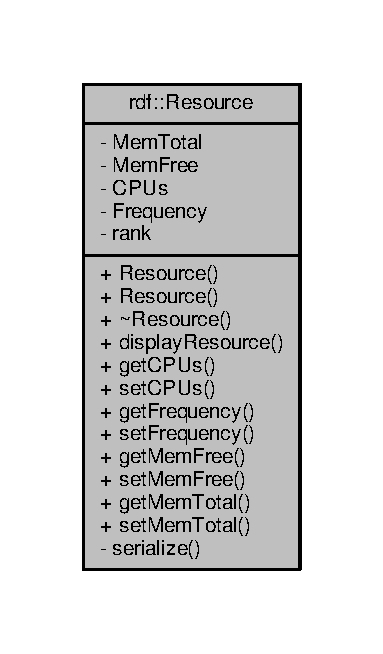
\includegraphics[width=184pt]{classrdf_1_1Resource__coll__graph}
\end{center}
\end{figure}
\subsection*{Public Member Functions}
\begin{DoxyCompactItemize}
\item 
\hyperlink{classrdf_1_1Resource_a6429643c9dc30ee324e10230203bfc19}{Resource} ()
\item 
\hyperlink{classrdf_1_1Resource_a05795b56fdd9f7850faaa26db68da378}{Resource} (const \hyperlink{classrdf_1_1Resource}{Resource} \&orig)
\item 
virtual \hyperlink{classrdf_1_1Resource_a1172ca19c641a1cdef69dadfbd71e135}{$\sim$\+Resource} ()
\item 
void \hyperlink{classrdf_1_1Resource_a494a37b398f88c9180215f7d2a56104a}{display\+Resource} ()
\item 
int \hyperlink{classrdf_1_1Resource_ad1d552c80195c2d60054bcb7aed1c3a0}{get\+C\+P\+Us} () const 
\item 
void \hyperlink{classrdf_1_1Resource_acde532c88486296bea5ae2420a981364}{set\+C\+P\+Us} (int \hyperlink{classrdf_1_1Resource_aa26913be707d9845b9c3ba180febe043}{C\+P\+Us})
\item 
int \hyperlink{classrdf_1_1Resource_adf18e6ac1a7707277a3dbc322acd082a}{get\+Frequency} () const 
\item 
void \hyperlink{classrdf_1_1Resource_a41df357db31501e5dbc0e78d347efc3e}{set\+Frequency} (int \hyperlink{classrdf_1_1Resource_ab5f7c94360292b32006f95e4a718decb}{Frequency})
\item 
int \hyperlink{classrdf_1_1Resource_a776692d45e08c13c1d3cbd8ef7ce9c5b}{get\+Mem\+Free} () const 
\item 
void \hyperlink{classrdf_1_1Resource_a91e688e3f3ea4ccd462887b687f7b14c}{set\+Mem\+Free} (int \hyperlink{classrdf_1_1Resource_a6fa4758d8e1cbc6315073e204bfcae7a}{Mem\+Free})
\item 
int \hyperlink{classrdf_1_1Resource_a6b082c36d255a097879d81ee347145a5}{get\+Mem\+Total} () const 
\item 
void \hyperlink{classrdf_1_1Resource_a316a34c2dd6758f3125e7f424b3f35ba}{set\+Mem\+Total} (int \hyperlink{classrdf_1_1Resource_a37ff1f3b7071c2cdd5dcfa39ed0c7174}{Mem\+Total})
\end{DoxyCompactItemize}
\subsection*{Private Member Functions}
\begin{DoxyCompactItemize}
\item 
{\footnotesize template$<$class Archive $>$ }\\void \hyperlink{classrdf_1_1Resource_adfedf0fbbd8025004e21d87d46dc7abf}{serialize} (Archive \&ar, const unsigned int version)
\end{DoxyCompactItemize}
\subsection*{Private Attributes}
\begin{DoxyCompactItemize}
\item 
int \hyperlink{classrdf_1_1Resource_a37ff1f3b7071c2cdd5dcfa39ed0c7174}{Mem\+Total}
\item 
int \hyperlink{classrdf_1_1Resource_a6fa4758d8e1cbc6315073e204bfcae7a}{Mem\+Free}
\item 
int \hyperlink{classrdf_1_1Resource_aa26913be707d9845b9c3ba180febe043}{C\+P\+Us}
\item 
int \hyperlink{classrdf_1_1Resource_ab5f7c94360292b32006f95e4a718decb}{Frequency}
\item 
int \hyperlink{classrdf_1_1Resource_abbff4961e68af1fe21b676b5d6d82146}{rank}
\end{DoxyCompactItemize}
\subsection*{Friends}
\begin{DoxyCompactItemize}
\item 
class \hyperlink{classrdf_1_1Resource_ac98d07dd8f7b70e16ccb9a01abf56b9c}{boost\+::serialization\+::access}
\end{DoxyCompactItemize}


\subsection{Constructor \& Destructor Documentation}
\index{rdf\+::\+Resource@{rdf\+::\+Resource}!Resource@{Resource}}
\index{Resource@{Resource}!rdf\+::\+Resource@{rdf\+::\+Resource}}
\subsubsection[{\texorpdfstring{Resource()}{Resource()}}]{\setlength{\rightskip}{0pt plus 5cm}rdf\+::\+Resource\+::\+Resource (
\begin{DoxyParamCaption}
{}
\end{DoxyParamCaption}
)}\hypertarget{classrdf_1_1Resource_a6429643c9dc30ee324e10230203bfc19}{}\label{classrdf_1_1Resource_a6429643c9dc30ee324e10230203bfc19}

\begin{DoxyCode}
16                       \{
17 \}
\end{DoxyCode}
\index{rdf\+::\+Resource@{rdf\+::\+Resource}!Resource@{Resource}}
\index{Resource@{Resource}!rdf\+::\+Resource@{rdf\+::\+Resource}}
\subsubsection[{\texorpdfstring{Resource(const Resource \&orig)}{Resource(const Resource &orig)}}]{\setlength{\rightskip}{0pt plus 5cm}rdf\+::\+Resource\+::\+Resource (
\begin{DoxyParamCaption}
\item[{const {\bf Resource} \&}]{orig}
\end{DoxyParamCaption}
)}\hypertarget{classrdf_1_1Resource_a05795b56fdd9f7850faaa26db68da378}{}\label{classrdf_1_1Resource_a05795b56fdd9f7850faaa26db68da378}


References C\+P\+Us, Frequency, Mem\+Free, and Mem\+Total.


\begin{DoxyCode}
19                                           \{
20     \hyperlink{classrdf_1_1Resource_a6fa4758d8e1cbc6315073e204bfcae7a}{MemFree}     =   orig.MemFree;
21     \hyperlink{classrdf_1_1Resource_a37ff1f3b7071c2cdd5dcfa39ed0c7174}{MemTotal}    =   orig.MemTotal;
22     \hyperlink{classrdf_1_1Resource_ab5f7c94360292b32006f95e4a718decb}{Frequency}   =   orig.Frequency;
23     \hyperlink{classrdf_1_1Resource_aa26913be707d9845b9c3ba180febe043}{CPUs}        =   orig.CPUs;
24     
25 \}
\end{DoxyCode}
\index{rdf\+::\+Resource@{rdf\+::\+Resource}!````~Resource@{$\sim$\+Resource}}
\index{````~Resource@{$\sim$\+Resource}!rdf\+::\+Resource@{rdf\+::\+Resource}}
\subsubsection[{\texorpdfstring{$\sim$\+Resource()}{~Resource()}}]{\setlength{\rightskip}{0pt plus 5cm}rdf\+::\+Resource\+::$\sim$\+Resource (
\begin{DoxyParamCaption}
{}
\end{DoxyParamCaption}
)\hspace{0.3cm}{\ttfamily [virtual]}}\hypertarget{classrdf_1_1Resource_a1172ca19c641a1cdef69dadfbd71e135}{}\label{classrdf_1_1Resource_a1172ca19c641a1cdef69dadfbd71e135}

\begin{DoxyCode}
27                        \{
28 \}
\end{DoxyCode}


\subsection{Member Function Documentation}
\index{rdf\+::\+Resource@{rdf\+::\+Resource}!display\+Resource@{display\+Resource}}
\index{display\+Resource@{display\+Resource}!rdf\+::\+Resource@{rdf\+::\+Resource}}
\subsubsection[{\texorpdfstring{display\+Resource()}{displayResource()}}]{\setlength{\rightskip}{0pt plus 5cm}void rdf\+::\+Resource\+::display\+Resource (
\begin{DoxyParamCaption}
{}
\end{DoxyParamCaption}
)}\hypertarget{classrdf_1_1Resource_a494a37b398f88c9180215f7d2a56104a}{}\label{classrdf_1_1Resource_a494a37b398f88c9180215f7d2a56104a}


References C\+P\+Us, Frequency, Mem\+Free, and Mem\+Total.



Referenced by rdf\+::\+Distribution\+Manager\+::transfer\+Resources().


\begin{DoxyCode}
31                                  \{
32     std::cout << \textcolor{stringliteral}{"Memoria total: "}  <<  \hyperlink{classrdf_1_1Resource_a37ff1f3b7071c2cdd5dcfa39ed0c7174}{rdf::Resource::MemTotal} << \textcolor{stringliteral}{"\(\backslash\)n"};
33     std::cout << \textcolor{stringliteral}{"Memoria libre: "}  <<  \hyperlink{classrdf_1_1Resource_a6fa4758d8e1cbc6315073e204bfcae7a}{rdf::Resource::MemFree} << \textcolor{stringliteral}{"\(\backslash\)n"};
34     std::cout << \textcolor{stringliteral}{"Frecuencia: "}     <<  \hyperlink{classrdf_1_1Resource_ab5f7c94360292b32006f95e4a718decb}{rdf::Resource::Frequency} << \textcolor{stringliteral}{"\(\backslash\)n"};
35     std::cout << \textcolor{stringliteral}{"Numero de CPUs: "} <<  \hyperlink{classrdf_1_1Resource_aa26913be707d9845b9c3ba180febe043}{rdf::Resource::CPUs} << \textcolor{stringliteral}{"\(\backslash\)n"};
36 \}
\end{DoxyCode}
\index{rdf\+::\+Resource@{rdf\+::\+Resource}!get\+C\+P\+Us@{get\+C\+P\+Us}}
\index{get\+C\+P\+Us@{get\+C\+P\+Us}!rdf\+::\+Resource@{rdf\+::\+Resource}}
\subsubsection[{\texorpdfstring{get\+C\+P\+Us() const }{getCPUs() const }}]{\setlength{\rightskip}{0pt plus 5cm}int rdf\+::\+Resource\+::get\+C\+P\+Us (
\begin{DoxyParamCaption}
{}
\end{DoxyParamCaption}
) const\hspace{0.3cm}{\ttfamily [inline]}}\hypertarget{classrdf_1_1Resource_ad1d552c80195c2d60054bcb7aed1c3a0}{}\label{classrdf_1_1Resource_ad1d552c80195c2d60054bcb7aed1c3a0}


References C\+P\+Us.


\begin{DoxyCode}
47                                 \{
48                 \textcolor{keywordflow}{return} \hyperlink{classrdf_1_1Resource_aa26913be707d9845b9c3ba180febe043}{CPUs};
49             \}
\end{DoxyCode}
\index{rdf\+::\+Resource@{rdf\+::\+Resource}!get\+Frequency@{get\+Frequency}}
\index{get\+Frequency@{get\+Frequency}!rdf\+::\+Resource@{rdf\+::\+Resource}}
\subsubsection[{\texorpdfstring{get\+Frequency() const }{getFrequency() const }}]{\setlength{\rightskip}{0pt plus 5cm}int rdf\+::\+Resource\+::get\+Frequency (
\begin{DoxyParamCaption}
{}
\end{DoxyParamCaption}
) const\hspace{0.3cm}{\ttfamily [inline]}}\hypertarget{classrdf_1_1Resource_adf18e6ac1a7707277a3dbc322acd082a}{}\label{classrdf_1_1Resource_adf18e6ac1a7707277a3dbc322acd082a}


References Frequency.


\begin{DoxyCode}
55                                      \{
56                 \textcolor{keywordflow}{return} \hyperlink{classrdf_1_1Resource_ab5f7c94360292b32006f95e4a718decb}{Frequency};
57             \}
\end{DoxyCode}
\index{rdf\+::\+Resource@{rdf\+::\+Resource}!get\+Mem\+Free@{get\+Mem\+Free}}
\index{get\+Mem\+Free@{get\+Mem\+Free}!rdf\+::\+Resource@{rdf\+::\+Resource}}
\subsubsection[{\texorpdfstring{get\+Mem\+Free() const }{getMemFree() const }}]{\setlength{\rightskip}{0pt plus 5cm}int rdf\+::\+Resource\+::get\+Mem\+Free (
\begin{DoxyParamCaption}
{}
\end{DoxyParamCaption}
) const\hspace{0.3cm}{\ttfamily [inline]}}\hypertarget{classrdf_1_1Resource_a776692d45e08c13c1d3cbd8ef7ce9c5b}{}\label{classrdf_1_1Resource_a776692d45e08c13c1d3cbd8ef7ce9c5b}


References Mem\+Free.



Referenced by rdf\+::\+Image\+Dispatcher\+::analyze\+Resource().


\begin{DoxyCode}
63                                    \{
64                 \textcolor{keywordflow}{return} \hyperlink{classrdf_1_1Resource_a6fa4758d8e1cbc6315073e204bfcae7a}{MemFree};
65             \}
\end{DoxyCode}
\index{rdf\+::\+Resource@{rdf\+::\+Resource}!get\+Mem\+Total@{get\+Mem\+Total}}
\index{get\+Mem\+Total@{get\+Mem\+Total}!rdf\+::\+Resource@{rdf\+::\+Resource}}
\subsubsection[{\texorpdfstring{get\+Mem\+Total() const }{getMemTotal() const }}]{\setlength{\rightskip}{0pt plus 5cm}int rdf\+::\+Resource\+::get\+Mem\+Total (
\begin{DoxyParamCaption}
{}
\end{DoxyParamCaption}
) const\hspace{0.3cm}{\ttfamily [inline]}}\hypertarget{classrdf_1_1Resource_a6b082c36d255a097879d81ee347145a5}{}\label{classrdf_1_1Resource_a6b082c36d255a097879d81ee347145a5}


References Mem\+Total.


\begin{DoxyCode}
71                                     \{
72                 \textcolor{keywordflow}{return} \hyperlink{classrdf_1_1Resource_a37ff1f3b7071c2cdd5dcfa39ed0c7174}{MemTotal};
73             \}
\end{DoxyCode}
\index{rdf\+::\+Resource@{rdf\+::\+Resource}!serialize@{serialize}}
\index{serialize@{serialize}!rdf\+::\+Resource@{rdf\+::\+Resource}}
\subsubsection[{\texorpdfstring{serialize(\+Archive \&ar, const unsigned int version)}{serialize(Archive &ar, const unsigned int version)}}]{\setlength{\rightskip}{0pt plus 5cm}template$<$class Archive $>$ void rdf\+::\+Resource\+::serialize (
\begin{DoxyParamCaption}
\item[{Archive \&}]{ar, }
\item[{const unsigned int}]{version}
\end{DoxyParamCaption}
)\hspace{0.3cm}{\ttfamily [inline]}, {\ttfamily [private]}}\hypertarget{classrdf_1_1Resource_adfedf0fbbd8025004e21d87d46dc7abf}{}\label{classrdf_1_1Resource_adfedf0fbbd8025004e21d87d46dc7abf}


References C\+P\+Us, Frequency, Mem\+Free, Mem\+Total, and rank.


\begin{DoxyCode}
27                 \{
28                     ar & \hyperlink{classrdf_1_1Resource_a37ff1f3b7071c2cdd5dcfa39ed0c7174}{MemTotal};
29                     ar & \hyperlink{classrdf_1_1Resource_a6fa4758d8e1cbc6315073e204bfcae7a}{MemFree};
30                     ar & \hyperlink{classrdf_1_1Resource_aa26913be707d9845b9c3ba180febe043}{CPUs};
31                     ar & \hyperlink{classrdf_1_1Resource_ab5f7c94360292b32006f95e4a718decb}{Frequency};
32                     ar & \hyperlink{classrdf_1_1Resource_abbff4961e68af1fe21b676b5d6d82146}{rank};
33             \}
\end{DoxyCode}
\index{rdf\+::\+Resource@{rdf\+::\+Resource}!set\+C\+P\+Us@{set\+C\+P\+Us}}
\index{set\+C\+P\+Us@{set\+C\+P\+Us}!rdf\+::\+Resource@{rdf\+::\+Resource}}
\subsubsection[{\texorpdfstring{set\+C\+P\+Us(int C\+P\+Us)}{setCPUs(int CPUs)}}]{\setlength{\rightskip}{0pt plus 5cm}void rdf\+::\+Resource\+::set\+C\+P\+Us (
\begin{DoxyParamCaption}
\item[{int}]{C\+P\+Us}
\end{DoxyParamCaption}
)\hspace{0.3cm}{\ttfamily [inline]}}\hypertarget{classrdf_1_1Resource_acde532c88486296bea5ae2420a981364}{}\label{classrdf_1_1Resource_acde532c88486296bea5ae2420a981364}


References C\+P\+Us.



Referenced by Resources\+::create\+Objet().


\begin{DoxyCode}
51                                    \{
52                 this->\hyperlink{classrdf_1_1Resource_aa26913be707d9845b9c3ba180febe043}{CPUs} = \hyperlink{classrdf_1_1Resource_aa26913be707d9845b9c3ba180febe043}{CPUs};
53             \}
\end{DoxyCode}
\index{rdf\+::\+Resource@{rdf\+::\+Resource}!set\+Frequency@{set\+Frequency}}
\index{set\+Frequency@{set\+Frequency}!rdf\+::\+Resource@{rdf\+::\+Resource}}
\subsubsection[{\texorpdfstring{set\+Frequency(int Frequency)}{setFrequency(int Frequency)}}]{\setlength{\rightskip}{0pt plus 5cm}void rdf\+::\+Resource\+::set\+Frequency (
\begin{DoxyParamCaption}
\item[{int}]{Frequency}
\end{DoxyParamCaption}
)\hspace{0.3cm}{\ttfamily [inline]}}\hypertarget{classrdf_1_1Resource_a41df357db31501e5dbc0e78d347efc3e}{}\label{classrdf_1_1Resource_a41df357db31501e5dbc0e78d347efc3e}


References Frequency.



Referenced by Resources\+::create\+Objet().


\begin{DoxyCode}
59                                              \{
60                 this->\hyperlink{classrdf_1_1Resource_ab5f7c94360292b32006f95e4a718decb}{Frequency} = \hyperlink{classrdf_1_1Resource_ab5f7c94360292b32006f95e4a718decb}{Frequency};
61             \}
\end{DoxyCode}
\index{rdf\+::\+Resource@{rdf\+::\+Resource}!set\+Mem\+Free@{set\+Mem\+Free}}
\index{set\+Mem\+Free@{set\+Mem\+Free}!rdf\+::\+Resource@{rdf\+::\+Resource}}
\subsubsection[{\texorpdfstring{set\+Mem\+Free(int Mem\+Free)}{setMemFree(int MemFree)}}]{\setlength{\rightskip}{0pt plus 5cm}void rdf\+::\+Resource\+::set\+Mem\+Free (
\begin{DoxyParamCaption}
\item[{int}]{Mem\+Free}
\end{DoxyParamCaption}
)\hspace{0.3cm}{\ttfamily [inline]}}\hypertarget{classrdf_1_1Resource_a91e688e3f3ea4ccd462887b687f7b14c}{}\label{classrdf_1_1Resource_a91e688e3f3ea4ccd462887b687f7b14c}


References Mem\+Free.



Referenced by Resources\+::create\+Objet().


\begin{DoxyCode}
67                                          \{
68                 this->\hyperlink{classrdf_1_1Resource_a6fa4758d8e1cbc6315073e204bfcae7a}{MemFree} = \hyperlink{classrdf_1_1Resource_a6fa4758d8e1cbc6315073e204bfcae7a}{MemFree};
69             \}
\end{DoxyCode}
\index{rdf\+::\+Resource@{rdf\+::\+Resource}!set\+Mem\+Total@{set\+Mem\+Total}}
\index{set\+Mem\+Total@{set\+Mem\+Total}!rdf\+::\+Resource@{rdf\+::\+Resource}}
\subsubsection[{\texorpdfstring{set\+Mem\+Total(int Mem\+Total)}{setMemTotal(int MemTotal)}}]{\setlength{\rightskip}{0pt plus 5cm}void rdf\+::\+Resource\+::set\+Mem\+Total (
\begin{DoxyParamCaption}
\item[{int}]{Mem\+Total}
\end{DoxyParamCaption}
)\hspace{0.3cm}{\ttfamily [inline]}}\hypertarget{classrdf_1_1Resource_a316a34c2dd6758f3125e7f424b3f35ba}{}\label{classrdf_1_1Resource_a316a34c2dd6758f3125e7f424b3f35ba}


References Mem\+Total.



Referenced by Resources\+::create\+Objet().


\begin{DoxyCode}
75                                            \{
76                 this->\hyperlink{classrdf_1_1Resource_a37ff1f3b7071c2cdd5dcfa39ed0c7174}{MemTotal} = \hyperlink{classrdf_1_1Resource_a37ff1f3b7071c2cdd5dcfa39ed0c7174}{MemTotal};
77             \}
\end{DoxyCode}


\subsection{Friends And Related Function Documentation}
\index{rdf\+::\+Resource@{rdf\+::\+Resource}!boost\+::serialization\+::access@{boost\+::serialization\+::access}}
\index{boost\+::serialization\+::access@{boost\+::serialization\+::access}!rdf\+::\+Resource@{rdf\+::\+Resource}}
\subsubsection[{\texorpdfstring{boost\+::serialization\+::access}{boost::serialization::access}}]{\setlength{\rightskip}{0pt plus 5cm}friend class boost\+::serialization\+::access\hspace{0.3cm}{\ttfamily [friend]}}\hypertarget{classrdf_1_1Resource_ac98d07dd8f7b70e16ccb9a01abf56b9c}{}\label{classrdf_1_1Resource_ac98d07dd8f7b70e16ccb9a01abf56b9c}


\subsection{Member Data Documentation}
\index{rdf\+::\+Resource@{rdf\+::\+Resource}!C\+P\+Us@{C\+P\+Us}}
\index{C\+P\+Us@{C\+P\+Us}!rdf\+::\+Resource@{rdf\+::\+Resource}}
\subsubsection[{\texorpdfstring{C\+P\+Us}{CPUs}}]{\setlength{\rightskip}{0pt plus 5cm}int rdf\+::\+Resource\+::\+C\+P\+Us\hspace{0.3cm}{\ttfamily [private]}}\hypertarget{classrdf_1_1Resource_aa26913be707d9845b9c3ba180febe043}{}\label{classrdf_1_1Resource_aa26913be707d9845b9c3ba180febe043}


Referenced by display\+Resource(), get\+C\+P\+Us(), Resource(), serialize(), and set\+C\+P\+Us().

\index{rdf\+::\+Resource@{rdf\+::\+Resource}!Frequency@{Frequency}}
\index{Frequency@{Frequency}!rdf\+::\+Resource@{rdf\+::\+Resource}}
\subsubsection[{\texorpdfstring{Frequency}{Frequency}}]{\setlength{\rightskip}{0pt plus 5cm}int rdf\+::\+Resource\+::\+Frequency\hspace{0.3cm}{\ttfamily [private]}}\hypertarget{classrdf_1_1Resource_ab5f7c94360292b32006f95e4a718decb}{}\label{classrdf_1_1Resource_ab5f7c94360292b32006f95e4a718decb}


Referenced by display\+Resource(), get\+Frequency(), Resource(), serialize(), and set\+Frequency().

\index{rdf\+::\+Resource@{rdf\+::\+Resource}!Mem\+Free@{Mem\+Free}}
\index{Mem\+Free@{Mem\+Free}!rdf\+::\+Resource@{rdf\+::\+Resource}}
\subsubsection[{\texorpdfstring{Mem\+Free}{MemFree}}]{\setlength{\rightskip}{0pt plus 5cm}int rdf\+::\+Resource\+::\+Mem\+Free\hspace{0.3cm}{\ttfamily [private]}}\hypertarget{classrdf_1_1Resource_a6fa4758d8e1cbc6315073e204bfcae7a}{}\label{classrdf_1_1Resource_a6fa4758d8e1cbc6315073e204bfcae7a}


Referenced by display\+Resource(), get\+Mem\+Free(), Resource(), serialize(), and set\+Mem\+Free().

\index{rdf\+::\+Resource@{rdf\+::\+Resource}!Mem\+Total@{Mem\+Total}}
\index{Mem\+Total@{Mem\+Total}!rdf\+::\+Resource@{rdf\+::\+Resource}}
\subsubsection[{\texorpdfstring{Mem\+Total}{MemTotal}}]{\setlength{\rightskip}{0pt plus 5cm}int rdf\+::\+Resource\+::\+Mem\+Total\hspace{0.3cm}{\ttfamily [private]}}\hypertarget{classrdf_1_1Resource_a37ff1f3b7071c2cdd5dcfa39ed0c7174}{}\label{classrdf_1_1Resource_a37ff1f3b7071c2cdd5dcfa39ed0c7174}


Referenced by display\+Resource(), get\+Mem\+Total(), Resource(), serialize(), and set\+Mem\+Total().

\index{rdf\+::\+Resource@{rdf\+::\+Resource}!rank@{rank}}
\index{rank@{rank}!rdf\+::\+Resource@{rdf\+::\+Resource}}
\subsubsection[{\texorpdfstring{rank}{rank}}]{\setlength{\rightskip}{0pt plus 5cm}int rdf\+::\+Resource\+::rank\hspace{0.3cm}{\ttfamily [private]}}\hypertarget{classrdf_1_1Resource_abbff4961e68af1fe21b676b5d6d82146}{}\label{classrdf_1_1Resource_abbff4961e68af1fe21b676b5d6d82146}


Referenced by serialize().



The documentation for this class was generated from the following files\+:\begin{DoxyCompactItemize}
\item 
\hyperlink{Resource_8h}{Resource.\+h}\item 
\hyperlink{Resource_8cpp}{Resource.\+cpp}\end{DoxyCompactItemize}

\hypertarget{classResources}{}\section{Resources Class Reference}
\label{classResources}\index{Resources@{Resources}}


{\ttfamily \#include $<$Resources.\+h$>$}



Collaboration diagram for Resources\+:
\nopagebreak
\begin{figure}[H]
\begin{center}
\leavevmode
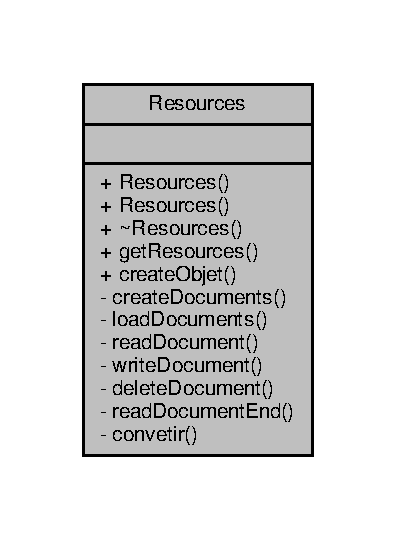
\includegraphics[width=190pt]{classResources__coll__graph}
\end{center}
\end{figure}
\subsection*{Public Member Functions}
\begin{DoxyCompactItemize}
\item 
\hyperlink{classResources_ab09435991b8c485f92e0aa1fd00828b9}{Resources} ()
\item 
\hyperlink{classResources_a1167e3cc0cfb0208c15b111537924ad9}{Resources} (const \hyperlink{classResources}{Resources} \&orig)
\item 
virtual \hyperlink{classResources_a5b75a9c6c6f5530ef807cce41cef81ee}{$\sim$\+Resources} ()
\item 
void \hyperlink{classResources_a9dfd1c5bb25dfe6d8d3fbb1d3b913bac}{get\+Resources} (std\+::vector$<$ std\+::string $>$ \&info\+Nodo\+Cluster)
\item 
void \hyperlink{classResources_ac1c8e38749088e3fc4211d9e3d72d18c}{create\+Objet} (std\+::vector$<$ std\+::string $>$ info\+Nodo\+Cluster, \hyperlink{classrdf_1_1Resource}{rdf\+::\+Resource} \&resources\+Nodo)
\end{DoxyCompactItemize}
\subsection*{Private Member Functions}
\begin{DoxyCompactItemize}
\item 
void \hyperlink{classResources_a1fc069e463d47d270d4b1b66560db7dd}{create\+Documents} ()
\item 
void \hyperlink{classResources_aa7fe3243ae9083d1d6c3a94e74ba9d91}{load\+Documents} (std\+::ifstream \&meminfo, std\+::ifstream \&cpuinfo)
\item 
void \hyperlink{classResources_a47e30c1968a197e5881a0ee82a639b60}{read\+Document} (std\+::ifstream \&file, std\+::string \&text, int tipo)
\item 
void \hyperlink{classResources_af5bb6af7ea6b20a4f6205146097aacee}{write\+Document} (std\+::string final)
\item 
void \hyperlink{classResources_a3e38b1670c66344d77dbae43071a3138}{delete\+Document} ()
\item 
void \hyperlink{classResources_a2bddda93d467f03795b4c8697c5a654a}{read\+Document\+End} (std\+::vector$<$ std\+::string $>$ \&vector)
\item 
void \hyperlink{classResources_adc6ae6012e41d5cadfefeaadafdd37d3}{convetir} ()
\end{DoxyCompactItemize}


\subsection{Constructor \& Destructor Documentation}
\index{Resources@{Resources}!Resources@{Resources}}
\index{Resources@{Resources}!Resources@{Resources}}
\subsubsection[{\texorpdfstring{Resources()}{Resources()}}]{\setlength{\rightskip}{0pt plus 5cm}Resources\+::\+Resources (
\begin{DoxyParamCaption}
{}
\end{DoxyParamCaption}
)}\hypertarget{classResources_ab09435991b8c485f92e0aa1fd00828b9}{}\label{classResources_ab09435991b8c485f92e0aa1fd00828b9}

\begin{DoxyCode}
19                      \{
20 \}
\end{DoxyCode}
\index{Resources@{Resources}!Resources@{Resources}}
\index{Resources@{Resources}!Resources@{Resources}}
\subsubsection[{\texorpdfstring{Resources(const Resources \&orig)}{Resources(const Resources &orig)}}]{\setlength{\rightskip}{0pt plus 5cm}Resources\+::\+Resources (
\begin{DoxyParamCaption}
\item[{const {\bf Resources} \&}]{orig}
\end{DoxyParamCaption}
)}\hypertarget{classResources_a1167e3cc0cfb0208c15b111537924ad9}{}\label{classResources_a1167e3cc0cfb0208c15b111537924ad9}

\begin{DoxyCode}
22                                           \{
23 \}
\end{DoxyCode}
\index{Resources@{Resources}!````~Resources@{$\sim$\+Resources}}
\index{````~Resources@{$\sim$\+Resources}!Resources@{Resources}}
\subsubsection[{\texorpdfstring{$\sim$\+Resources()}{~Resources()}}]{\setlength{\rightskip}{0pt plus 5cm}Resources\+::$\sim$\+Resources (
\begin{DoxyParamCaption}
{}
\end{DoxyParamCaption}
)\hspace{0.3cm}{\ttfamily [virtual]}}\hypertarget{classResources_a5b75a9c6c6f5530ef807cce41cef81ee}{}\label{classResources_a5b75a9c6c6f5530ef807cce41cef81ee}

\begin{DoxyCode}
25                       \{
26 \}
\end{DoxyCode}


\subsection{Member Function Documentation}
\index{Resources@{Resources}!convetir@{convetir}}
\index{convetir@{convetir}!Resources@{Resources}}
\subsubsection[{\texorpdfstring{convetir()}{convetir()}}]{\setlength{\rightskip}{0pt plus 5cm}void Resources\+::convetir (
\begin{DoxyParamCaption}
{}
\end{DoxyParamCaption}
)\hspace{0.3cm}{\ttfamily [private]}}\hypertarget{classResources_adc6ae6012e41d5cadfefeaadafdd37d3}{}\label{classResources_adc6ae6012e41d5cadfefeaadafdd37d3}


Referenced by get\+Resources().


\begin{DoxyCode}
51                          \{
52     std::ifstream meminfo, cpuinfo;
53     meminfo.open(\textcolor{stringliteral}{"meminfo.txt"});
54     cpuinfo.open(\textcolor{stringliteral}{"cpuinfo.txt"});
55     std::string mem, cpu;
56 
57     \textcolor{keywordtype}{char} c;
58     \textcolor{keywordflow}{if} (meminfo.is\_open()) \{
59         \textcolor{keywordflow}{while} (!meminfo.eof()) \{
60             meminfo >> c;
61             \textcolor{keywordflow}{if} (c == \textcolor{charliteral}{'$'}) \{
62                 mem.append(\textcolor{stringliteral}{"\(\backslash\)n"});
63             \} \textcolor{keywordflow}{else} \{
64                 mem += c;
65             \}
66         \}
67     \}
68 
69     \textcolor{keywordflow}{if} (cpuinfo.is\_open()) \{
70         \textcolor{keywordflow}{while} (!cpuinfo.eof()) \{
71             cpuinfo >> c;
72             \textcolor{keywordflow}{if} (c == \textcolor{charliteral}{'$'}) \{
73                 cpu.append(\textcolor{stringliteral}{"\(\backslash\)n"});
74             \} \textcolor{keywordflow}{else} \{
75                 cpu += c;
76             \}
77         \}
78     \}
79     
80     meminfo.close();
81     cpuinfo.close();
82     
83     std::ofstream omeminfo, ocpuinfo;
84     omeminfo.open(\textcolor{stringliteral}{"meminfo.txt"});
85     ocpuinfo.open(\textcolor{stringliteral}{"cpuinfo.txt"});
86     
87     omeminfo << mem;
88     ocpuinfo << cpu;
89     
90     omeminfo.close();
91     ocpuinfo.close();
92 
93 \}
\end{DoxyCode}
\index{Resources@{Resources}!create\+Documents@{create\+Documents}}
\index{create\+Documents@{create\+Documents}!Resources@{Resources}}
\subsubsection[{\texorpdfstring{create\+Documents()}{createDocuments()}}]{\setlength{\rightskip}{0pt plus 5cm}void Resources\+::create\+Documents (
\begin{DoxyParamCaption}
{}
\end{DoxyParamCaption}
)\hspace{0.3cm}{\ttfamily [private]}}\hypertarget{classResources_a1fc069e463d47d270d4b1b66560db7dd}{}\label{classResources_a1fc069e463d47d270d4b1b66560db7dd}


Referenced by get\+Resources().


\begin{DoxyCode}
95                                 \{
96     system(\textcolor{stringliteral}{"echo $(cat -E /proc/meminfo) >meminfo.txt"});
97     system(\textcolor{stringliteral}{"echo $(cat -E /proc/cpuinfo) >cpuinfo.txt"});
98 \}
\end{DoxyCode}
\index{Resources@{Resources}!create\+Objet@{create\+Objet}}
\index{create\+Objet@{create\+Objet}!Resources@{Resources}}
\subsubsection[{\texorpdfstring{create\+Objet(std\+::vector$<$ std\+::string $>$ info\+Nodo\+Cluster, rdf\+::\+Resource \&resources\+Nodo)}{createObjet(std::vector< std::string > infoNodoCluster, rdf::Resource &resourcesNodo)}}]{\setlength{\rightskip}{0pt plus 5cm}void Resources\+::create\+Objet (
\begin{DoxyParamCaption}
\item[{std\+::vector$<$ std\+::string $>$}]{info\+Nodo\+Cluster, }
\item[{{\bf rdf\+::\+Resource} \&}]{resources\+Nodo}
\end{DoxyParamCaption}
)}\hypertarget{classResources_ac1c8e38749088e3fc4211d9e3d72d18c}{}\label{classResources_ac1c8e38749088e3fc4211d9e3d72d18c}


References rdf\+::\+Resource\+::set\+C\+P\+Us(), rdf\+::\+Resource\+::set\+Frequency(), rdf\+::\+Resource\+::set\+Mem\+Free(), and rdf\+::\+Resource\+::set\+Mem\+Total().



Referenced by rdf\+::\+Distribution\+Manager\+::transfer\+Resources().


\begin{DoxyCode}
168                                                                                            \{
169     
170     std::string memtotal = infoNodoCluster[1];
171     std::string valueMemTotal = \textcolor{stringliteral}{""};
172     \textcolor{keywordtype}{bool} readValueTotal = \textcolor{keyword}{false};
173     \textcolor{keywordflow}{for} (\textcolor{keywordtype}{unsigned} \textcolor{keywordtype}{int} i = 0; i < memtotal.size(); i++) \{
174         \textcolor{keywordflow}{if}(memtotal[i] == \textcolor{charliteral}{'k'})\{
175             readValueTotal = \textcolor{keyword}{false};
176         \}
177         \textcolor{keywordflow}{if} (readValueTotal) \{ 
178             valueMemTotal = valueMemTotal + memtotal[i]; 
179         \}
180         \textcolor{keywordflow}{if}(memtotal[i] == \textcolor{charliteral}{':'})\{
181             readValueTotal = \textcolor{keyword}{true};
182         \}
183 
184     \}
185 
186     std::string memfree = infoNodoCluster[2];
187     std::string valueMemFree = \textcolor{stringliteral}{""};
188     \textcolor{keywordtype}{bool} readValueFree = \textcolor{keyword}{false};
189     \textcolor{keywordflow}{for} (\textcolor{keywordtype}{unsigned} \textcolor{keywordtype}{int} i = 0; i < memfree.size(); i++) \{
190         \textcolor{keywordflow}{if}(memfree[i] == \textcolor{charliteral}{'k'})\{
191             readValueFree = \textcolor{keyword}{false};
192         \}
193         \textcolor{keywordflow}{if} (readValueFree) \{ 
194             valueMemFree = valueMemFree + memfree[i]; 
195         \}
196         \textcolor{keywordflow}{if}(memfree[i] == \textcolor{charliteral}{':'})\{
197             readValueFree = \textcolor{keyword}{true};
198         \}
199     \}
200     
201     
202     
203     std::string frequency = infoNodoCluster[5];
204     std::string valueFrequency = \textcolor{stringliteral}{""};
205     \textcolor{keywordtype}{bool} readValueFrequency = \textcolor{keyword}{false};
206     \textcolor{keywordflow}{for} (\textcolor{keywordtype}{unsigned} \textcolor{keywordtype}{int} i = 0; i < frequency.size(); i++) \{
207         \textcolor{keywordflow}{if}(frequency[i] == \textcolor{charliteral}{'k'})\{
208             readValueFrequency = \textcolor{keyword}{false};
209         \}
210         \textcolor{keywordflow}{if} (readValueFrequency) \{ 
211             valueFrequency = valueFrequency + frequency[i]; 
212         \}
213         \textcolor{keywordflow}{if}(frequency[i] == \textcolor{charliteral}{':'})\{
214             readValueFrequency = \textcolor{keyword}{true};
215         \}
216     \}
217     
218     
219     
220     \textcolor{keywordtype}{int} cpus = 0; 
221     \textcolor{keywordflow}{for} (\textcolor{keywordtype}{unsigned} \textcolor{keywordtype}{int} i = 3; i < infoNodoCluster.size(); i++) \{
222         std::string valor = infoNodoCluster[i];
223         \textcolor{keywordflow}{if}(!valor.compare(0,9,\textcolor{stringliteral}{"processor"}))\{
224             cpus += 1;
225         \}
226     \}
227     
228     resourcesNodo.\hyperlink{classrdf_1_1Resource_acde532c88486296bea5ae2420a981364}{setCPUs}      (cpus);
229     resourcesNodo.\hyperlink{classrdf_1_1Resource_a41df357db31501e5dbc0e78d347efc3e}{setFrequency} (atoi(valueFrequency.c\_str()));
230     resourcesNodo.\hyperlink{classrdf_1_1Resource_a91e688e3f3ea4ccd462887b687f7b14c}{setMemFree}   (atoi(valueMemFree.c\_str()));
231     resourcesNodo.\hyperlink{classrdf_1_1Resource_a316a34c2dd6758f3125e7f424b3f35ba}{setMemTotal}  (atoi(valueMemTotal.c\_str()));
232     
233     
234     
235     
236 \}
\end{DoxyCode}
\index{Resources@{Resources}!delete\+Document@{delete\+Document}}
\index{delete\+Document@{delete\+Document}!Resources@{Resources}}
\subsubsection[{\texorpdfstring{delete\+Document()}{deleteDocument()}}]{\setlength{\rightskip}{0pt plus 5cm}void Resources\+::delete\+Document (
\begin{DoxyParamCaption}
{}
\end{DoxyParamCaption}
)\hspace{0.3cm}{\ttfamily [private]}}\hypertarget{classResources_a3e38b1670c66344d77dbae43071a3138}{}\label{classResources_a3e38b1670c66344d77dbae43071a3138}


Referenced by get\+Resources().


\begin{DoxyCode}
152                                \{
153     \textcolor{keyword}{remove}(\textcolor{stringliteral}{"meminfo.txt"});
154     \textcolor{keyword}{remove}(\textcolor{stringliteral}{"cpuinfo.txt"});
155 \}
\end{DoxyCode}
\index{Resources@{Resources}!get\+Resources@{get\+Resources}}
\index{get\+Resources@{get\+Resources}!Resources@{Resources}}
\subsubsection[{\texorpdfstring{get\+Resources(std\+::vector$<$ std\+::string $>$ \&info\+Nodo\+Cluster)}{getResources(std::vector< std::string > &infoNodoCluster)}}]{\setlength{\rightskip}{0pt plus 5cm}void Resources\+::get\+Resources (
\begin{DoxyParamCaption}
\item[{std\+::vector$<$ std\+::string $>$ \&}]{info\+Nodo\+Cluster}
\end{DoxyParamCaption}
)}\hypertarget{classResources_a9dfd1c5bb25dfe6d8d3fbb1d3b913bac}{}\label{classResources_a9dfd1c5bb25dfe6d8d3fbb1d3b913bac}


References convetir(), create\+Documents(), delete\+Document(), load\+Documents(), read\+Document(), read\+Document\+End(), and write\+Document().



Referenced by rdf\+::\+Distribution\+Manager\+::transfer\+Resources().


\begin{DoxyCode}
28                                                                   \{
29     std::ifstream meminfo, cpuinfo;
30     std::string all = \textcolor{stringliteral}{""};
31     std::vector<std::string> infoNodoClusterTemp;
32     \hyperlink{classResources_a1fc069e463d47d270d4b1b66560db7dd}{createDocuments}();
33     \hyperlink{classResources_adc6ae6012e41d5cadfefeaadafdd37d3}{convetir}();
34 
35     \hyperlink{classResources_aa7fe3243ae9083d1d6c3a94e74ba9d91}{loadDocuments}(meminfo, cpuinfo);
36 
37     \hyperlink{classResources_a47e30c1968a197e5881a0ee82a639b60}{readDocument}(meminfo, all, 0);
38     \hyperlink{classResources_a47e30c1968a197e5881a0ee82a639b60}{readDocument}(cpuinfo, all, 1);
39     
40     meminfo.close();
41     cpuinfo.close();
42     \hyperlink{classResources_af5bb6af7ea6b20a4f6205146097aacee}{writeDocument}(all);
43 
44     \hyperlink{classResources_a3e38b1670c66344d77dbae43071a3138}{deleteDocument}();
45 
46     \hyperlink{classResources_a2bddda93d467f03795b4c8697c5a654a}{readDocumentEnd}(infoNodoClusterTemp);
47 
48     infoNodoCluster = infoNodoClusterTemp;
49 \}
\end{DoxyCode}
\index{Resources@{Resources}!load\+Documents@{load\+Documents}}
\index{load\+Documents@{load\+Documents}!Resources@{Resources}}
\subsubsection[{\texorpdfstring{load\+Documents(std\+::ifstream \&meminfo, std\+::ifstream \&cpuinfo)}{loadDocuments(std::ifstream &meminfo, std::ifstream &cpuinfo)}}]{\setlength{\rightskip}{0pt plus 5cm}void Resources\+::load\+Documents (
\begin{DoxyParamCaption}
\item[{std\+::ifstream \&}]{meminfo, }
\item[{std\+::ifstream \&}]{cpuinfo}
\end{DoxyParamCaption}
)\hspace{0.3cm}{\ttfamily [private]}}\hypertarget{classResources_aa7fe3243ae9083d1d6c3a94e74ba9d91}{}\label{classResources_aa7fe3243ae9083d1d6c3a94e74ba9d91}


Referenced by get\+Resources().


\begin{DoxyCode}
100                                                                         \{
101     meminfo.open(\textcolor{stringliteral}{"meminfo.txt"});
102     cpuinfo.open(\textcolor{stringliteral}{"cpuinfo.txt"});
103 \}
\end{DoxyCode}
\index{Resources@{Resources}!read\+Document@{read\+Document}}
\index{read\+Document@{read\+Document}!Resources@{Resources}}
\subsubsection[{\texorpdfstring{read\+Document(std\+::ifstream \&file, std\+::string \&text, int tipo)}{readDocument(std::ifstream &file, std::string &text, int tipo)}}]{\setlength{\rightskip}{0pt plus 5cm}void Resources\+::read\+Document (
\begin{DoxyParamCaption}
\item[{std\+::ifstream \&}]{file, }
\item[{std\+::string \&}]{text, }
\item[{int}]{tipo}
\end{DoxyParamCaption}
)\hspace{0.3cm}{\ttfamily [private]}}\hypertarget{classResources_a47e30c1968a197e5881a0ee82a639b60}{}\label{classResources_a47e30c1968a197e5881a0ee82a639b60}


Referenced by get\+Resources().


\begin{DoxyCode}
105                                                                          \{
106     std::string line;
107     std::string temporal = \textcolor{stringliteral}{""};
108     \textcolor{keywordflow}{if} (tipo == 0) \{
109         temporal = \textcolor{stringliteral}{"Memory\_info\(\backslash\)n"};
110         \textcolor{keywordflow}{while} (!file.eof()) \{
111             getline(file, line); \textcolor{comment}{//Lee la linea}
112             std::string value;
113             std::stringstream check1(line);
114             \textcolor{keywordflow}{while} (getline(check1, value, \textcolor{charliteral}{' '})) \{
115                 \textcolor{keywordflow}{if} (value.compare(0,9,\textcolor{stringliteral}{"MemTotal:"}) == 0) \{ \textcolor{comment}{//value == "MemTotal:"}
116                     temporal += line + \textcolor{charliteral}{'\(\backslash\)n'};
117                     
118                 \} \textcolor{keywordflow}{else} \textcolor{keywordflow}{if} (value.compare(0,8,\textcolor{stringliteral}{"MemFree:"})== 0) \{
119                     temporal += line + \textcolor{charliteral}{'\(\backslash\)n'};
120                     
121                 \}
122             \}
123         \}
124     \} \textcolor{keywordflow}{else} \{
125         temporal += \textcolor{stringliteral}{"CPU\_info\(\backslash\)n"};
126         \textcolor{keywordflow}{while} (!file.eof()) \{
127             getline(file, line); \textcolor{comment}{//Lee la linea}
128             std::string value;
129             std::stringstream check1(line);
130             
131             \textcolor{keywordflow}{while} (getline(check1, value, \textcolor{charliteral}{' '})) \{
132                 \textcolor{keywordflow}{if} (value.compare(0,9,\textcolor{stringliteral}{"processor"}) == 0) \{
133                     temporal += line + \textcolor{charliteral}{'\(\backslash\)n'}; 
134                 \} \textcolor{keywordflow}{else} \textcolor{keywordflow}{if} (value.compare(0,6,\textcolor{stringliteral}{"cpuMHz"}) == 0) \{
135                     temporal += line + \textcolor{charliteral}{'\(\backslash\)n'};
136                 \} \textcolor{keywordflow}{else} \textcolor{keywordflow}{if} (value.compare(0,8,\textcolor{stringliteral}{"cpucores"}) == 0) \{
137                     temporal += line + \textcolor{charliteral}{'\(\backslash\)n'};
138                 \}
139             \}
140         \}
141     \}
142     text += temporal;
143 \}
\end{DoxyCode}
\index{Resources@{Resources}!read\+Document\+End@{read\+Document\+End}}
\index{read\+Document\+End@{read\+Document\+End}!Resources@{Resources}}
\subsubsection[{\texorpdfstring{read\+Document\+End(std\+::vector$<$ std\+::string $>$ \&vector)}{readDocumentEnd(std::vector< std::string > &vector)}}]{\setlength{\rightskip}{0pt plus 5cm}void Resources\+::read\+Document\+End (
\begin{DoxyParamCaption}
\item[{std\+::vector$<$ std\+::string $>$ \&}]{vector}
\end{DoxyParamCaption}
)\hspace{0.3cm}{\ttfamily [private]}}\hypertarget{classResources_a2bddda93d467f03795b4c8697c5a654a}{}\label{classResources_a2bddda93d467f03795b4c8697c5a654a}


Referenced by get\+Resources().


\begin{DoxyCode}
157                                                             \{
158     std::ifstream file;
159     std::string line;
160     file.open(\textcolor{stringliteral}{"Resources.txt"}, std::ifstream::in);
161     \textcolor{comment}{//Leer el archivo hasta que termine.}
162     \textcolor{keywordflow}{while} (!file.eof()) \{
163         getline(file, line); \textcolor{comment}{//Lee la linea}
164         vector.push\_back(line); \textcolor{comment}{//agrega la linea al vector}
165     \}
166 \}
\end{DoxyCode}
\index{Resources@{Resources}!write\+Document@{write\+Document}}
\index{write\+Document@{write\+Document}!Resources@{Resources}}
\subsubsection[{\texorpdfstring{write\+Document(std\+::string final)}{writeDocument(std::string final)}}]{\setlength{\rightskip}{0pt plus 5cm}void Resources\+::write\+Document (
\begin{DoxyParamCaption}
\item[{std\+::string}]{final}
\end{DoxyParamCaption}
)\hspace{0.3cm}{\ttfamily [private]}}\hypertarget{classResources_af5bb6af7ea6b20a4f6205146097aacee}{}\label{classResources_af5bb6af7ea6b20a4f6205146097aacee}


Referenced by get\+Resources().


\begin{DoxyCode}
145                                              \{
146     std::ofstream file;
147     file.open(\textcolor{stringliteral}{"Resources.txt"});
148     file << \textcolor{keyword}{final};
149     file.close();
150 \}
\end{DoxyCode}


The documentation for this class was generated from the following files\+:\begin{DoxyCompactItemize}
\item 
\hyperlink{Resources_8h}{Resources.\+h}\item 
\hyperlink{Resources_8cpp}{Resources.\+cpp}\end{DoxyCompactItemize}

\hypertarget{classScheduler}{}\section{Scheduler Class Reference}
\label{classScheduler}\index{Scheduler@{Scheduler}}


{\ttfamily \#include $<$Scheduler.\+h$>$}



Collaboration diagram for Scheduler\+:
\nopagebreak
\begin{figure}[H]
\begin{center}
\leavevmode
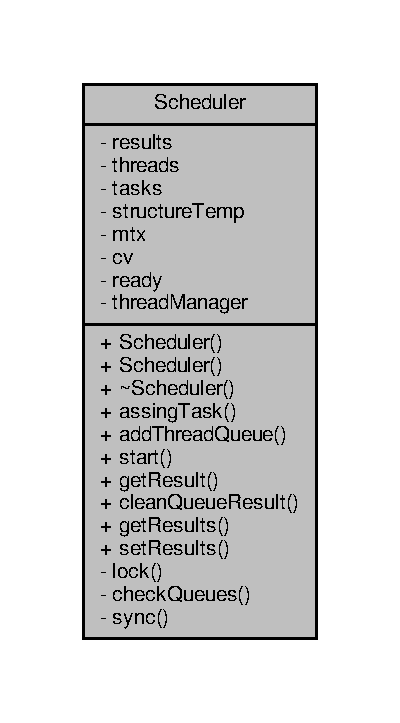
\includegraphics[width=192pt]{classScheduler__coll__graph}
\end{center}
\end{figure}
\subsection*{Public Member Functions}
\begin{DoxyCompactItemize}
\item 
\hyperlink{classScheduler_a3b61aac11466cd45ae42ab8c2b0013f6}{Scheduler} ()
\item 
\hyperlink{classScheduler_ae42ce9b6724e40c750ef6619bb35bee3}{Scheduler} (const \hyperlink{classScheduler}{Scheduler} \&orig)
\item 
virtual \hyperlink{classScheduler_afc8187779b46f64039d3ffa58f0dbe51}{$\sim$\+Scheduler} ()
\item 
void \hyperlink{classScheduler_a67fd277bb0cf15c2aa437cd1f7ed6e0a}{assing\+Task} (std\+::vector$<$ \hyperlink{structEstructura_1_1Node}{Estructura\+::\+Node} $>$ structure, \hyperlink{classrdf_1_1Task}{rdf\+::\+Task} \&task)
\item 
void \hyperlink{classScheduler_abc04c3760251ca922019db0cec5f0d50}{add\+Thread\+Queue} (\hyperlink{classQueueThread}{Queue\+Thread} thread)
\item 
void \hyperlink{classScheduler_a63a264c69136bace160286ef30ed0c11}{start} ()
\item 
void \hyperlink{classScheduler_a200281a389579bc17faf446f52efc801}{get\+Result} (std\+::queue$<$ \hyperlink{classrdf_1_1NodeResult}{rdf\+::\+Node\+Result} $>$ \&\hyperlink{classScheduler_a93faf0df4ed95016cdb5224bd2725c3f}{results})
\item 
void \hyperlink{classScheduler_a0f1e295c22d686d6888a22ebdc57869f}{clean\+Queue\+Result} ()
\item 
std\+::queue$<$ \hyperlink{classrdf_1_1NodeResult}{rdf\+::\+Node\+Result} $>$ \hyperlink{classScheduler_a8864f6b658cf4d2a6d9d78a84c6d81f7}{get\+Results} () const 
\item 
void \hyperlink{classScheduler_a9e9839fbddf57961b055e32144db7d9a}{set\+Results} (std\+::queue$<$ \hyperlink{classrdf_1_1NodeResult}{rdf\+::\+Node\+Result} $>$ \hyperlink{classScheduler_a93faf0df4ed95016cdb5224bd2725c3f}{results})
\end{DoxyCompactItemize}
\subsection*{Private Member Functions}
\begin{DoxyCompactItemize}
\item 
void \hyperlink{classScheduler_a903ad54edab99f678aef0f79e2b426f8}{lock} ()
\item 
void \hyperlink{classScheduler_a157e2d59b776d904c07c81d47af5d3df}{check\+Queues} (std\+::vector$<$ \hyperlink{structEstructura_1_1Node}{Estructura\+::\+Node} $>$ structure, std\+::priority\+\_\+queue$<$ \hyperlink{classrdf_1_1Task}{rdf\+::\+Task} $>$ \hyperlink{classScheduler_adbcdf6edd31a2e8e088eb5bc91b4465e}{tasks})
\item 
void \hyperlink{classScheduler_a6f86da54c4ec3f2566ce7251d59c8302}{sync} ()
\end{DoxyCompactItemize}
\subsection*{Private Attributes}
\begin{DoxyCompactItemize}
\item 
std\+::queue$<$ \hyperlink{classrdf_1_1NodeResult}{rdf\+::\+Node\+Result} $>$ \hyperlink{classScheduler_a93faf0df4ed95016cdb5224bd2725c3f}{results}
\item 
std\+::queue$<$ \hyperlink{classQueueThread}{Queue\+Thread} $>$ \hyperlink{classScheduler_a99f7fcd7cb3977cb7e76232a01aceffe}{threads}
\item 
std\+::priority\+\_\+queue$<$ \hyperlink{classrdf_1_1Task}{rdf\+::\+Task} $>$ \hyperlink{classScheduler_adbcdf6edd31a2e8e088eb5bc91b4465e}{tasks}
\item 
std\+::vector$<$ \hyperlink{structEstructura_1_1Node}{Estructura\+::\+Node} $>$ \hyperlink{classScheduler_a0603b1b04040b5e71cf3a945a1ec09b9}{structure\+Temp}
\item 
std\+::mutex \hyperlink{classScheduler_a19d05f87e9815e222ec52bcbfa81e435}{mtx}
\item 
std\+::condition\+\_\+variable \hyperlink{classScheduler_ac0bfe3868a5c8ba5205a8a50f6459083}{cv}
\item 
bool \hyperlink{classScheduler_a9a7edcef4b80171f8bb4b2802a3bc31f}{ready} = false
\item 
std\+::thread \hyperlink{classScheduler_ad1cbfa2210145f7d50c2648845707e68}{thread\+Manager}
\end{DoxyCompactItemize}


\subsection{Constructor \& Destructor Documentation}
\index{Scheduler@{Scheduler}!Scheduler@{Scheduler}}
\index{Scheduler@{Scheduler}!Scheduler@{Scheduler}}
\subsubsection[{\texorpdfstring{Scheduler()}{Scheduler()}}]{\setlength{\rightskip}{0pt plus 5cm}Scheduler\+::\+Scheduler (
\begin{DoxyParamCaption}
{}
\end{DoxyParamCaption}
)}\hypertarget{classScheduler_a3b61aac11466cd45ae42ab8c2b0013f6}{}\label{classScheduler_a3b61aac11466cd45ae42ab8c2b0013f6}


References threads.


\begin{DoxyCode}
18                      \{
19 
20     \textcolor{keywordflow}{for} (\textcolor{keywordtype}{int} i = 0; i < 8; i++) \{
21         \hyperlink{classQueueThread}{QueueThread} thread;
22         \hyperlink{classScheduler_a99f7fcd7cb3977cb7e76232a01aceffe}{Scheduler::threads}.push(thread);
23     \}
24 \}
\end{DoxyCode}
\index{Scheduler@{Scheduler}!Scheduler@{Scheduler}}
\index{Scheduler@{Scheduler}!Scheduler@{Scheduler}}
\subsubsection[{\texorpdfstring{Scheduler(const Scheduler \&orig)}{Scheduler(const Scheduler &orig)}}]{\setlength{\rightskip}{0pt plus 5cm}Scheduler\+::\+Scheduler (
\begin{DoxyParamCaption}
\item[{const {\bf Scheduler} \&}]{orig}
\end{DoxyParamCaption}
)}\hypertarget{classScheduler_ae42ce9b6724e40c750ef6619bb35bee3}{}\label{classScheduler_ae42ce9b6724e40c750ef6619bb35bee3}

\begin{DoxyCode}
26                                           \{
27 \}
\end{DoxyCode}
\index{Scheduler@{Scheduler}!````~Scheduler@{$\sim$\+Scheduler}}
\index{````~Scheduler@{$\sim$\+Scheduler}!Scheduler@{Scheduler}}
\subsubsection[{\texorpdfstring{$\sim$\+Scheduler()}{~Scheduler()}}]{\setlength{\rightskip}{0pt plus 5cm}Scheduler\+::$\sim$\+Scheduler (
\begin{DoxyParamCaption}
{}
\end{DoxyParamCaption}
)\hspace{0.3cm}{\ttfamily [virtual]}}\hypertarget{classScheduler_afc8187779b46f64039d3ffa58f0dbe51}{}\label{classScheduler_afc8187779b46f64039d3ffa58f0dbe51}

\begin{DoxyCode}
29                       \{
30 \}
\end{DoxyCode}


\subsection{Member Function Documentation}
\index{Scheduler@{Scheduler}!add\+Thread\+Queue@{add\+Thread\+Queue}}
\index{add\+Thread\+Queue@{add\+Thread\+Queue}!Scheduler@{Scheduler}}
\subsubsection[{\texorpdfstring{add\+Thread\+Queue(\+Queue\+Thread thread)}{addThreadQueue(QueueThread thread)}}]{\setlength{\rightskip}{0pt plus 5cm}void Scheduler\+::add\+Thread\+Queue (
\begin{DoxyParamCaption}
\item[{{\bf Queue\+Thread}}]{thread}
\end{DoxyParamCaption}
)}\hypertarget{classScheduler_abc04c3760251ca922019db0cec5f0d50}{}\label{classScheduler_abc04c3760251ca922019db0cec5f0d50}


References threads.



Referenced by check\+Queues().


\begin{DoxyCode}
117                                                  \{
118     \hyperlink{classQueueThread}{QueueThread} threadTem;
119     \hyperlink{classScheduler_a99f7fcd7cb3977cb7e76232a01aceffe}{Scheduler::threads}.push(thread);
120 \}
\end{DoxyCode}
\index{Scheduler@{Scheduler}!assing\+Task@{assing\+Task}}
\index{assing\+Task@{assing\+Task}!Scheduler@{Scheduler}}
\subsubsection[{\texorpdfstring{assing\+Task(std\+::vector$<$ Estructura\+::\+Node $>$ structure, rdf\+::\+Task \&task)}{assingTask(std::vector< Estructura::Node > structure, rdf::Task &task)}}]{\setlength{\rightskip}{0pt plus 5cm}void Scheduler\+::assing\+Task (
\begin{DoxyParamCaption}
\item[{std\+::vector$<$ {\bf Estructura\+::\+Node} $>$}]{structure, }
\item[{{\bf rdf\+::\+Task} \&}]{task}
\end{DoxyParamCaption}
)}\hypertarget{classScheduler_a67fd277bb0cf15c2aa437cd1f7ed6e0a}{}\label{classScheduler_a67fd277bb0cf15c2aa437cd1f7ed6e0a}


References check\+Queues(), and tasks.


\begin{DoxyCode}
38                                                                              \{
39 
40     \textcolor{comment}{//structureTemp = structure;}
41     \hyperlink{classScheduler_adbcdf6edd31a2e8e088eb5bc91b4465e}{tasks}.push(task);
42     \hyperlink{classScheduler_a157e2d59b776d904c07c81d47af5d3df}{checkQueues}(structure, \hyperlink{classScheduler_adbcdf6edd31a2e8e088eb5bc91b4465e}{tasks});
43 
44 \}
\end{DoxyCode}
\index{Scheduler@{Scheduler}!check\+Queues@{check\+Queues}}
\index{check\+Queues@{check\+Queues}!Scheduler@{Scheduler}}
\subsubsection[{\texorpdfstring{check\+Queues(std\+::vector$<$ Estructura\+::\+Node $>$ structure, std\+::priority\+\_\+queue$<$ rdf\+::\+Task $>$ tasks)}{checkQueues(std::vector< Estructura::Node > structure, std::priority_queue< rdf::Task > tasks)}}]{\setlength{\rightskip}{0pt plus 5cm}void Scheduler\+::check\+Queues (
\begin{DoxyParamCaption}
\item[{std\+::vector$<$ {\bf Estructura\+::\+Node} $>$}]{structure, }
\item[{std\+::priority\+\_\+queue$<$ {\bf rdf\+::\+Task} $>$}]{tasks}
\end{DoxyParamCaption}
)\hspace{0.3cm}{\ttfamily [private]}}\hypertarget{classScheduler_a157e2d59b776d904c07c81d47af5d3df}{}\label{classScheduler_a157e2d59b776d904c07c81d47af5d3df}


References add\+Thread\+Queue(), Queue\+Thread\+::connect(), rdf\+::\+Node\+Result\+::get\+Matrix\+Results(), rdf\+::\+Node\+Result\+::get\+Task(), rdf\+::\+Node\+Result\+::is\+Status(), lock(), ready, results, rdf\+::\+Node\+Result\+::set\+Status(), rdf\+::\+Node\+Result\+::set\+Task(), rdf\+::\+Task\+::show\+Task(), sync(), tasks, thread\+Manager, and threads.



Referenced by assing\+Task().


\begin{DoxyCode}
46                                                                                                  \{
47 
48     \textcolor{keywordflow}{if} (!\hyperlink{classScheduler_adbcdf6edd31a2e8e088eb5bc91b4465e}{tasks}.empty()) \{
49 
50         \hyperlink{classrdf_1_1Task}{rdf::Task} task = \hyperlink{classScheduler_adbcdf6edd31a2e8e088eb5bc91b4465e}{Scheduler::tasks}.top();
51         \hyperlink{classScheduler_adbcdf6edd31a2e8e088eb5bc91b4465e}{Scheduler::tasks}.pop();
52         \hyperlink{classScheduler_a6f86da54c4ec3f2566ce7251d59c8302}{sync}();
53 
54 
55 
56         \textcolor{keywordflow}{if} (\hyperlink{classScheduler_a9a7edcef4b80171f8bb4b2802a3bc31f}{ready} && \hyperlink{classScheduler_a99f7fcd7cb3977cb7e76232a01aceffe}{threads}.size() > 0) \{
57 
58             \textcolor{comment}{//objeto node result}
59             \hyperlink{classrdf_1_1NodeResult}{rdf::NodeResult} *nodeResult  = \textcolor{keyword}{new} \hyperlink{classrdf_1_1NodeResult}{rdf::NodeResult}();
60             \textcolor{comment}{//rdf::NodeResult nodeResultTemp;}
61             nodeResult->\hyperlink{classrdf_1_1NodeResult_a29f9794788bb251bccddb5377bb78eba}{setTask}(task);
62             \hyperlink{classQueueThread}{QueueThread} thread = \hyperlink{classScheduler_a99f7fcd7cb3977cb7e76232a01aceffe}{Scheduler::threads}.front();
63             \hyperlink{classScheduler_a99f7fcd7cb3977cb7e76232a01aceffe}{Scheduler::threads}.pop();
64             \hyperlink{classScheduler_ad1cbfa2210145f7d50c2648845707e68}{threadManager} = std::thread(&\hyperlink{classQueueThread_a873d5d9edf446f44467518c8fbde1800}{QueueThread::connect}, 
      \hyperlink{classQueueThread}{QueueThread}(), structure, task, \hyperlink{classScheduler_adbcdf6edd31a2e8e088eb5bc91b4465e}{tasks}, std::ref(*nodeResult));
65             \textcolor{keywordflow}{if} (\hyperlink{classScheduler_ad1cbfa2210145f7d50c2648845707e68}{threadManager}.joinable())
66                 \hyperlink{classScheduler_ad1cbfa2210145f7d50c2648845707e68}{threadManager}.join();
67             \hyperlink{classScheduler_a9a7edcef4b80171f8bb4b2802a3bc31f}{ready} = \textcolor{keyword}{false};
68             \hyperlink{classScheduler_abc04c3760251ca922019db0cec5f0d50}{addThreadQueue}(thread);
69             std::cout << \textcolor{stringliteral}{"Task: "};
70             nodeResult->\hyperlink{classrdf_1_1NodeResult_a564d581492a48333ed9796f6fd4b8c6a}{getTask}().\hyperlink{classrdf_1_1Task_aed5f96455f9684078a5fa8fce849d197}{showTask}();
71             std::cout << \textcolor{stringliteral}{"Results: \(\backslash\)n"};
72             nodeResult->\hyperlink{classrdf_1_1NodeResult_ab0d07def4def30c0875602c5e3dde208}{getMatrixResults}().Print();
73             nodeResult->\hyperlink{classrdf_1_1NodeResult_a52df0a39fb56beec66feacf802639b2c}{setStatus}(0);
74             \textcolor{comment}{//nodeResult.setMatrixResults(nodeResultTemp.getMatrixResults());}
75             \hyperlink{classScheduler_a93faf0df4ed95016cdb5224bd2725c3f}{results}.push(*nodeResult);
76             
77             std::cout << \hyperlink{classScheduler_a93faf0df4ed95016cdb5224bd2725c3f}{results}.size() << \textcolor{stringliteral}{" \(\backslash\)n"};
78             \textcolor{keywordflow}{for} (\textcolor{keywordtype}{int} i = 0; i < \hyperlink{classScheduler_a93faf0df4ed95016cdb5224bd2725c3f}{results}.size(); i++) \{
79                  \hyperlink{classrdf_1_1NodeResult}{rdf::NodeResult} nodetemp = \hyperlink{classScheduler_a93faf0df4ed95016cdb5224bd2725c3f}{results}.front();
80                  \hyperlink{classScheduler_a93faf0df4ed95016cdb5224bd2725c3f}{results}.pop();
81                  nodetemp.\hyperlink{classrdf_1_1NodeResult_a564d581492a48333ed9796f6fd4b8c6a}{getTask}().\hyperlink{classrdf_1_1Task_aed5f96455f9684078a5fa8fce849d197}{showTask}();
82                  
83                  std::cout << \textcolor{stringliteral}{"
      \_\_\_\_\_\_\_\_\_\_\_\_\_\_\_\_\_\_\_\_\_\_\_\_\_\_\_\_\_\_\_\_\_\_\_\_\_\_\_\_\_\_\_\_\_\_\_\_\_\_\_\_\_\_\_\_\_\_\_\_\_\_\_\_\_\_\_\_\_\_\_\_\_\_\_\_\_\_\_ \(\backslash\)n "};
84                  nodetemp.\hyperlink{classrdf_1_1NodeResult_ab0d07def4def30c0875602c5e3dde208}{getMatrixResults}().Print();
85                  std::cout << \textcolor{stringliteral}{"CE: "} << nodetemp.\hyperlink{classrdf_1_1NodeResult_a09ad0a96c0591976f73ef288eff195c7}{isStatus}() << \textcolor{stringliteral}{"\(\backslash\)n"};
86                  std::cout << \textcolor{stringliteral}{"
      \_\_\_\_\_\_\_\_\_\_\_\_\_\_\_\_\_\_\_\_\_\_\_\_\_\_\_\_\_\_****************\_\_\_\_\_\_\_\_\_\_\_\_\_\_\_\_\_\_\_\_\_\_\_\_\_\_\_\_\_\_\_\_\_\_\(\backslash\)n "};
87 
88             \}
89 
90             \textcolor{comment}{//nodeResult.getMatrixResults().Print();}
91             \textcolor{comment}{//results.push(nodeResult);}
92 
93         \} \textcolor{keywordflow}{else} \{
94             \hyperlink{classScheduler_a903ad54edab99f678aef0f79e2b426f8}{lock}();
95         \}
96 
97     \} \textcolor{keywordflow}{else} \{
98 
99         \textcolor{keywordflow}{if} (\hyperlink{classScheduler_a99f7fcd7cb3977cb7e76232a01aceffe}{threads}.size() != 0) \{
100         \}
101     \}
102 \}
\end{DoxyCode}
\index{Scheduler@{Scheduler}!clean\+Queue\+Result@{clean\+Queue\+Result}}
\index{clean\+Queue\+Result@{clean\+Queue\+Result}!Scheduler@{Scheduler}}
\subsubsection[{\texorpdfstring{clean\+Queue\+Result()}{cleanQueueResult()}}]{\setlength{\rightskip}{0pt plus 5cm}void Scheduler\+::clean\+Queue\+Result (
\begin{DoxyParamCaption}
{}
\end{DoxyParamCaption}
)}\hypertarget{classScheduler_a0f1e295c22d686d6888a22ebdc57869f}{}\label{classScheduler_a0f1e295c22d686d6888a22ebdc57869f}


References results.


\begin{DoxyCode}
126                                 \{
127     \textcolor{keywordflow}{for} (\textcolor{keywordtype}{int} i = 0; i < \hyperlink{classScheduler_a93faf0df4ed95016cdb5224bd2725c3f}{results}.size(); i++) \{
128         \hyperlink{classScheduler_a93faf0df4ed95016cdb5224bd2725c3f}{results}.pop();
129     \}
130 \}
\end{DoxyCode}
\index{Scheduler@{Scheduler}!get\+Result@{get\+Result}}
\index{get\+Result@{get\+Result}!Scheduler@{Scheduler}}
\subsubsection[{\texorpdfstring{get\+Result(std\+::queue$<$ rdf\+::\+Node\+Result $>$ \&results)}{getResult(std::queue< rdf::NodeResult > &results)}}]{\setlength{\rightskip}{0pt plus 5cm}void Scheduler\+::get\+Result (
\begin{DoxyParamCaption}
\item[{std\+::queue$<$ {\bf rdf\+::\+Node\+Result} $>$ \&}]{results}
\end{DoxyParamCaption}
)}\hypertarget{classScheduler_a200281a389579bc17faf446f52efc801}{}\label{classScheduler_a200281a389579bc17faf446f52efc801}


References results.


\begin{DoxyCode}
122                                                          \{
123     \hyperlink{classScheduler_a93faf0df4ed95016cdb5224bd2725c3f}{results} = \hyperlink{classScheduler_a93faf0df4ed95016cdb5224bd2725c3f}{Scheduler::results};
124 \}
\end{DoxyCode}
\index{Scheduler@{Scheduler}!get\+Results@{get\+Results}}
\index{get\+Results@{get\+Results}!Scheduler@{Scheduler}}
\subsubsection[{\texorpdfstring{get\+Results() const }{getResults() const }}]{\setlength{\rightskip}{0pt plus 5cm}std\+::queue$<${\bf rdf\+::\+Node\+Result}$>$ Scheduler\+::get\+Results (
\begin{DoxyParamCaption}
{}
\end{DoxyParamCaption}
) const\hspace{0.3cm}{\ttfamily [inline]}}\hypertarget{classScheduler_a8864f6b658cf4d2a6d9d78a84c6d81f7}{}\label{classScheduler_a8864f6b658cf4d2a6d9d78a84c6d81f7}


References results.



Referenced by rdf\+::\+Distribution\+Manager\+::sending\+Results().


\begin{DoxyCode}
51                                                \{
52         \textcolor{keywordflow}{return} \hyperlink{classScheduler_a93faf0df4ed95016cdb5224bd2725c3f}{results};
53     \}
\end{DoxyCode}
\index{Scheduler@{Scheduler}!lock@{lock}}
\index{lock@{lock}!Scheduler@{Scheduler}}
\subsubsection[{\texorpdfstring{lock()}{lock()}}]{\setlength{\rightskip}{0pt plus 5cm}void Scheduler\+::lock (
\begin{DoxyParamCaption}
{}
\end{DoxyParamCaption}
)\hspace{0.3cm}{\ttfamily [private]}}\hypertarget{classScheduler_a903ad54edab99f678aef0f79e2b426f8}{}\label{classScheduler_a903ad54edab99f678aef0f79e2b426f8}


References cv, mtx, and ready.



Referenced by check\+Queues().


\begin{DoxyCode}
110                      \{
111     std::unique\_lock<std::mutex> lck(\hyperlink{classScheduler_a19d05f87e9815e222ec52bcbfa81e435}{mtx});
112     \textcolor{keywordflow}{while} (!\hyperlink{classScheduler_a9a7edcef4b80171f8bb4b2802a3bc31f}{ready}) \{
113         \hyperlink{classScheduler_ac0bfe3868a5c8ba5205a8a50f6459083}{cv}.wait(lck);
114     \}
115 \}
\end{DoxyCode}
\index{Scheduler@{Scheduler}!set\+Results@{set\+Results}}
\index{set\+Results@{set\+Results}!Scheduler@{Scheduler}}
\subsubsection[{\texorpdfstring{set\+Results(std\+::queue$<$ rdf\+::\+Node\+Result $>$ results)}{setResults(std::queue< rdf::NodeResult > results)}}]{\setlength{\rightskip}{0pt plus 5cm}void Scheduler\+::set\+Results (
\begin{DoxyParamCaption}
\item[{std\+::queue$<$ {\bf rdf\+::\+Node\+Result} $>$}]{results}
\end{DoxyParamCaption}
)\hspace{0.3cm}{\ttfamily [inline]}}\hypertarget{classScheduler_a9e9839fbddf57961b055e32144db7d9a}{}\label{classScheduler_a9e9839fbddf57961b055e32144db7d9a}


References results.


\begin{DoxyCode}
55                                                      \{
56         this->\hyperlink{classScheduler_a93faf0df4ed95016cdb5224bd2725c3f}{results} = \hyperlink{classScheduler_a93faf0df4ed95016cdb5224bd2725c3f}{results};
57     \}
\end{DoxyCode}
\index{Scheduler@{Scheduler}!start@{start}}
\index{start@{start}!Scheduler@{Scheduler}}
\subsubsection[{\texorpdfstring{start()}{start()}}]{\setlength{\rightskip}{0pt plus 5cm}void Scheduler\+::start (
\begin{DoxyParamCaption}
{}
\end{DoxyParamCaption}
)}\hypertarget{classScheduler_a63a264c69136bace160286ef30ed0c11}{}\label{classScheduler_a63a264c69136bace160286ef30ed0c11}

\begin{DoxyCode}
32                       \{
33     \textcolor{comment}{//threadManager = std::thread(&Scheduler::checkQueues, this, structureTemp, tasks);}
34     \textcolor{comment}{//rdf::Task task;}
35     \textcolor{comment}{//threadManager = std::thread(&QueueThread::connect,QueueThread(), structureTemp, task, tasks);}
36 \}
\end{DoxyCode}
\index{Scheduler@{Scheduler}!sync@{sync}}
\index{sync@{sync}!Scheduler@{Scheduler}}
\subsubsection[{\texorpdfstring{sync()}{sync()}}]{\setlength{\rightskip}{0pt plus 5cm}void Scheduler\+::sync (
\begin{DoxyParamCaption}
{}
\end{DoxyParamCaption}
)\hspace{0.3cm}{\ttfamily [private]}}\hypertarget{classScheduler_a6f86da54c4ec3f2566ce7251d59c8302}{}\label{classScheduler_a6f86da54c4ec3f2566ce7251d59c8302}


References cv, mtx, and ready.



Referenced by check\+Queues().


\begin{DoxyCode}
104                      \{
105     std::unique\_lock<std::mutex> lck(\hyperlink{classScheduler_a19d05f87e9815e222ec52bcbfa81e435}{mtx});
106     \hyperlink{classScheduler_a9a7edcef4b80171f8bb4b2802a3bc31f}{ready} = \textcolor{keyword}{true};
107     \hyperlink{classScheduler_ac0bfe3868a5c8ba5205a8a50f6459083}{cv}.notify\_one();
108 \}
\end{DoxyCode}


\subsection{Member Data Documentation}
\index{Scheduler@{Scheduler}!cv@{cv}}
\index{cv@{cv}!Scheduler@{Scheduler}}
\subsubsection[{\texorpdfstring{cv}{cv}}]{\setlength{\rightskip}{0pt plus 5cm}std\+::condition\+\_\+variable Scheduler\+::cv\hspace{0.3cm}{\ttfamily [private]}}\hypertarget{classScheduler_ac0bfe3868a5c8ba5205a8a50f6459083}{}\label{classScheduler_ac0bfe3868a5c8ba5205a8a50f6459083}


Referenced by lock(), and sync().

\index{Scheduler@{Scheduler}!mtx@{mtx}}
\index{mtx@{mtx}!Scheduler@{Scheduler}}
\subsubsection[{\texorpdfstring{mtx}{mtx}}]{\setlength{\rightskip}{0pt plus 5cm}std\+::mutex Scheduler\+::mtx\hspace{0.3cm}{\ttfamily [private]}}\hypertarget{classScheduler_a19d05f87e9815e222ec52bcbfa81e435}{}\label{classScheduler_a19d05f87e9815e222ec52bcbfa81e435}


Referenced by lock(), and sync().

\index{Scheduler@{Scheduler}!ready@{ready}}
\index{ready@{ready}!Scheduler@{Scheduler}}
\subsubsection[{\texorpdfstring{ready}{ready}}]{\setlength{\rightskip}{0pt plus 5cm}bool Scheduler\+::ready = false\hspace{0.3cm}{\ttfamily [private]}}\hypertarget{classScheduler_a9a7edcef4b80171f8bb4b2802a3bc31f}{}\label{classScheduler_a9a7edcef4b80171f8bb4b2802a3bc31f}


Referenced by check\+Queues(), lock(), and sync().

\index{Scheduler@{Scheduler}!results@{results}}
\index{results@{results}!Scheduler@{Scheduler}}
\subsubsection[{\texorpdfstring{results}{results}}]{\setlength{\rightskip}{0pt plus 5cm}std\+::queue$<${\bf rdf\+::\+Node\+Result}$>$ Scheduler\+::results\hspace{0.3cm}{\ttfamily [private]}}\hypertarget{classScheduler_a93faf0df4ed95016cdb5224bd2725c3f}{}\label{classScheduler_a93faf0df4ed95016cdb5224bd2725c3f}


Referenced by check\+Queues(), clean\+Queue\+Result(), get\+Result(), get\+Results(), and set\+Results().

\index{Scheduler@{Scheduler}!structure\+Temp@{structure\+Temp}}
\index{structure\+Temp@{structure\+Temp}!Scheduler@{Scheduler}}
\subsubsection[{\texorpdfstring{structure\+Temp}{structureTemp}}]{\setlength{\rightskip}{0pt plus 5cm}std\+::vector$<${\bf Estructura\+::\+Node}$>$ Scheduler\+::structure\+Temp\hspace{0.3cm}{\ttfamily [private]}}\hypertarget{classScheduler_a0603b1b04040b5e71cf3a945a1ec09b9}{}\label{classScheduler_a0603b1b04040b5e71cf3a945a1ec09b9}
\index{Scheduler@{Scheduler}!tasks@{tasks}}
\index{tasks@{tasks}!Scheduler@{Scheduler}}
\subsubsection[{\texorpdfstring{tasks}{tasks}}]{\setlength{\rightskip}{0pt plus 5cm}std\+::priority\+\_\+queue$<${\bf rdf\+::\+Task}$>$ Scheduler\+::tasks\hspace{0.3cm}{\ttfamily [private]}}\hypertarget{classScheduler_adbcdf6edd31a2e8e088eb5bc91b4465e}{}\label{classScheduler_adbcdf6edd31a2e8e088eb5bc91b4465e}


Referenced by assing\+Task(), and check\+Queues().

\index{Scheduler@{Scheduler}!thread\+Manager@{thread\+Manager}}
\index{thread\+Manager@{thread\+Manager}!Scheduler@{Scheduler}}
\subsubsection[{\texorpdfstring{thread\+Manager}{threadManager}}]{\setlength{\rightskip}{0pt plus 5cm}std\+::thread Scheduler\+::thread\+Manager\hspace{0.3cm}{\ttfamily [private]}}\hypertarget{classScheduler_ad1cbfa2210145f7d50c2648845707e68}{}\label{classScheduler_ad1cbfa2210145f7d50c2648845707e68}


Referenced by check\+Queues().

\index{Scheduler@{Scheduler}!threads@{threads}}
\index{threads@{threads}!Scheduler@{Scheduler}}
\subsubsection[{\texorpdfstring{threads}{threads}}]{\setlength{\rightskip}{0pt plus 5cm}std\+::queue$<${\bf Queue\+Thread}$>$ Scheduler\+::threads\hspace{0.3cm}{\ttfamily [private]}}\hypertarget{classScheduler_a99f7fcd7cb3977cb7e76232a01aceffe}{}\label{classScheduler_a99f7fcd7cb3977cb7e76232a01aceffe}


Referenced by add\+Thread\+Queue(), check\+Queues(), and Scheduler().



The documentation for this class was generated from the following files\+:\begin{DoxyCompactItemize}
\item 
\hyperlink{Scheduler_8h}{Scheduler.\+h}\item 
\hyperlink{Scheduler_8cpp}{Scheduler.\+cpp}\end{DoxyCompactItemize}

\hypertarget{classStrategyImage}{}\section{Strategy\+Image Class Reference}
\label{classStrategyImage}\index{Strategy\+Image@{Strategy\+Image}}


{\ttfamily \#include $<$Strategy\+Image.\+h$>$}



Inheritance diagram for Strategy\+Image\+:
\nopagebreak
\begin{figure}[H]
\begin{center}
\leavevmode
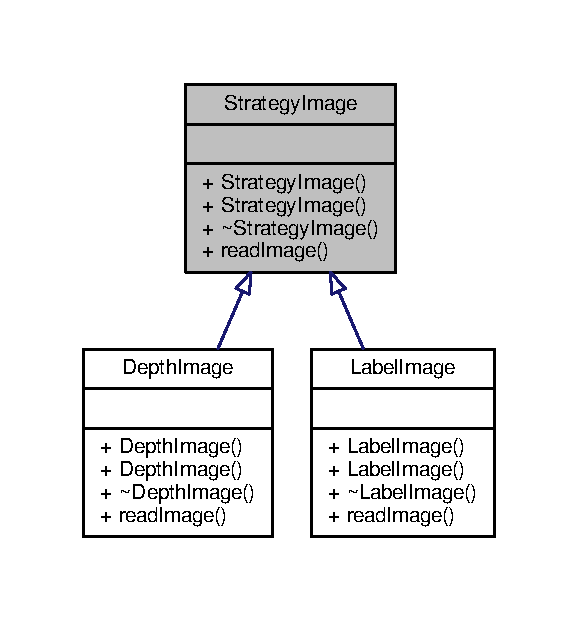
\includegraphics[width=278pt]{classStrategyImage__inherit__graph}
\end{center}
\end{figure}


Collaboration diagram for Strategy\+Image\+:
\nopagebreak
\begin{figure}[H]
\begin{center}
\leavevmode
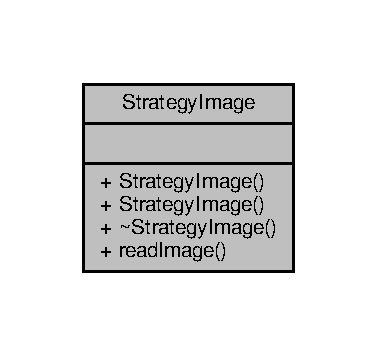
\includegraphics[width=181pt]{classStrategyImage__coll__graph}
\end{center}
\end{figure}
\subsection*{Public Member Functions}
\begin{DoxyCompactItemize}
\item 
\hyperlink{classStrategyImage_a84fd98378aaf8205424e67669b7d709b}{Strategy\+Image} ()
\item 
\hyperlink{classStrategyImage_a32561e112fe7fe08fa74ce986077f2c0}{Strategy\+Image} (const \hyperlink{classStrategyImage}{Strategy\+Image} \&orig)
\item 
virtual \hyperlink{classStrategyImage_a4a4e107957a7a97d73e160da121e7fb0}{$\sim$\+Strategy\+Image} ()
\item 
virtual void \hyperlink{classStrategyImage_aee857e79df483412f66b529417ddfd44}{read\+Image} (int heigth, int width, std\+::string direction, cv\+::\+Mat \&image)=0
\end{DoxyCompactItemize}


\subsection{Constructor \& Destructor Documentation}
\index{Strategy\+Image@{Strategy\+Image}!Strategy\+Image@{Strategy\+Image}}
\index{Strategy\+Image@{Strategy\+Image}!Strategy\+Image@{Strategy\+Image}}
\subsubsection[{\texorpdfstring{Strategy\+Image()}{StrategyImage()}}]{\setlength{\rightskip}{0pt plus 5cm}Strategy\+Image\+::\+Strategy\+Image (
\begin{DoxyParamCaption}
{}
\end{DoxyParamCaption}
)}\hypertarget{classStrategyImage_a84fd98378aaf8205424e67669b7d709b}{}\label{classStrategyImage_a84fd98378aaf8205424e67669b7d709b}

\begin{DoxyCode}
16                              \{
17 \}
\end{DoxyCode}
\index{Strategy\+Image@{Strategy\+Image}!Strategy\+Image@{Strategy\+Image}}
\index{Strategy\+Image@{Strategy\+Image}!Strategy\+Image@{Strategy\+Image}}
\subsubsection[{\texorpdfstring{Strategy\+Image(const Strategy\+Image \&orig)}{StrategyImage(const StrategyImage &orig)}}]{\setlength{\rightskip}{0pt plus 5cm}Strategy\+Image\+::\+Strategy\+Image (
\begin{DoxyParamCaption}
\item[{const {\bf Strategy\+Image} \&}]{orig}
\end{DoxyParamCaption}
)}\hypertarget{classStrategyImage_a32561e112fe7fe08fa74ce986077f2c0}{}\label{classStrategyImage_a32561e112fe7fe08fa74ce986077f2c0}

\begin{DoxyCode}
19                                                       \{
20 \}
\end{DoxyCode}
\index{Strategy\+Image@{Strategy\+Image}!````~Strategy\+Image@{$\sim$\+Strategy\+Image}}
\index{````~Strategy\+Image@{$\sim$\+Strategy\+Image}!Strategy\+Image@{Strategy\+Image}}
\subsubsection[{\texorpdfstring{$\sim$\+Strategy\+Image()}{~StrategyImage()}}]{\setlength{\rightskip}{0pt plus 5cm}Strategy\+Image\+::$\sim$\+Strategy\+Image (
\begin{DoxyParamCaption}
{}
\end{DoxyParamCaption}
)\hspace{0.3cm}{\ttfamily [virtual]}}\hypertarget{classStrategyImage_a4a4e107957a7a97d73e160da121e7fb0}{}\label{classStrategyImage_a4a4e107957a7a97d73e160da121e7fb0}

\begin{DoxyCode}
22                               \{
23 \}\end{DoxyCode}


\subsection{Member Function Documentation}
\index{Strategy\+Image@{Strategy\+Image}!read\+Image@{read\+Image}}
\index{read\+Image@{read\+Image}!Strategy\+Image@{Strategy\+Image}}
\subsubsection[{\texorpdfstring{read\+Image(int heigth, int width, std\+::string direction, cv\+::\+Mat \&image)=0}{readImage(int heigth, int width, std::string direction, cv::Mat &image)=0}}]{\setlength{\rightskip}{0pt plus 5cm}virtual void Strategy\+Image\+::read\+Image (
\begin{DoxyParamCaption}
\item[{int}]{heigth, }
\item[{int}]{width, }
\item[{std\+::string}]{direction, }
\item[{cv\+::\+Mat \&}]{image}
\end{DoxyParamCaption}
)\hspace{0.3cm}{\ttfamily [pure virtual]}}\hypertarget{classStrategyImage_aee857e79df483412f66b529417ddfd44}{}\label{classStrategyImage_aee857e79df483412f66b529417ddfd44}


Implemented in \hyperlink{classLabelImage_a1adf267dcf7b64f1ef085e434edae7a0}{Label\+Image}, and \hyperlink{classDepthImage_a07e7b06393e869a1cc3c5b39d2dcdad0}{Depth\+Image}.



Referenced by Collection\+::read\+Image().



The documentation for this class was generated from the following files\+:\begin{DoxyCompactItemize}
\item 
\hyperlink{StrategyImage_8h}{Strategy\+Image.\+h}\item 
\hyperlink{StrategyImage_8cpp}{Strategy\+Image.\+cpp}\end{DoxyCompactItemize}

\hypertarget{classrdf_1_1Task}{}\section{rdf\+:\+:Task Class Reference}
\label{classrdf_1_1Task}\index{rdf\+::\+Task@{rdf\+::\+Task}}


{\ttfamily \#include $<$Task.\+h$>$}



Collaboration diagram for rdf\+:\+:Task\+:
\nopagebreak
\begin{figure}[H]
\begin{center}
\leavevmode
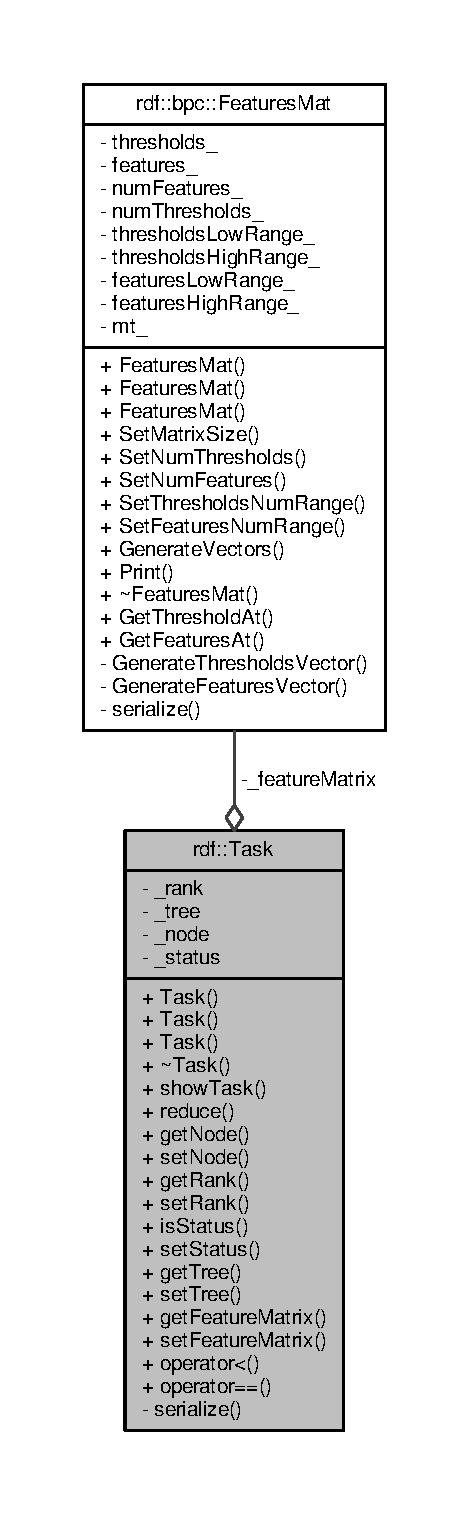
\includegraphics[height=550pt]{classrdf_1_1Task__coll__graph}
\end{center}
\end{figure}
\subsection*{Public Member Functions}
\begin{DoxyCompactItemize}
\item 
\hyperlink{classrdf_1_1Task_a8457894b8d8fa131f71a7d517ba7bf74}{Task} ()
\item 
\hyperlink{classrdf_1_1Task_ae22d87a6bbaa872fb9a2d7b635e23017}{Task} (int \hyperlink{classrdf_1_1Task_a66806490016907e1acd9ad771811e4d5}{\+\_\+rank}, int \hyperlink{classrdf_1_1Task_a3986abc1d8a8c79bde8d7525c6faa0bd}{\+\_\+tree}, int \hyperlink{classrdf_1_1Task_ab505294f64848a3ee104c9efa45528b5}{\+\_\+node}, bool \hyperlink{classrdf_1_1Task_a43face20dfc0d868ef400070d0fd43bb}{\+\_\+status})
\item 
\hyperlink{classrdf_1_1Task_a1858fac2f9519af47ac11fcb742d4866}{Task} (const \hyperlink{classrdf_1_1Task}{Task} \&orig)
\item 
virtual \hyperlink{classrdf_1_1Task_aad3f295247fa60106899c5ee5b9eae8a}{$\sim$\+Task} ()
\item 
void \hyperlink{classrdf_1_1Task_aed5f96455f9684078a5fa8fce849d197}{show\+Task} ()
\item 
void \hyperlink{classrdf_1_1Task_aee187dbed7bb9b900114920162f9866b}{reduce} (\hyperlink{classrdf_1_1Task}{Task} \&p\+Task1)
\item 
int \hyperlink{classrdf_1_1Task_abed5b1d313483299a04f0ccb63901c54}{get\+Node} () const 
\item 
void \hyperlink{classrdf_1_1Task_aa7667e08b39f5b6cae63aa0abeb4c412}{set\+Node} (int \hyperlink{classrdf_1_1Task_ab505294f64848a3ee104c9efa45528b5}{\+\_\+node})
\item 
int \hyperlink{classrdf_1_1Task_ab1bcd01480e2c381541b6346f15cf4b7}{get\+Rank} () const 
\item 
void \hyperlink{classrdf_1_1Task_aa55d27b31ed812e31e21fa5676208f1b}{set\+Rank} (int \hyperlink{classrdf_1_1Task_a66806490016907e1acd9ad771811e4d5}{\+\_\+rank})
\item 
bool \hyperlink{classrdf_1_1Task_a2d78d32594b0c8f76a599cc3883211c7}{is\+Status} () const 
\item 
void \hyperlink{classrdf_1_1Task_af030aac32a3943f2cd0fb22c8e964071}{set\+Status} (bool \hyperlink{classrdf_1_1Task_a43face20dfc0d868ef400070d0fd43bb}{\+\_\+status})
\item 
int \hyperlink{classrdf_1_1Task_a942297717d39a25db9ed8636ef72dca1}{get\+Tree} () const 
\item 
void \hyperlink{classrdf_1_1Task_ad7948910883a02524a0975d47c1827a7}{set\+Tree} (int \hyperlink{classrdf_1_1Task_a3986abc1d8a8c79bde8d7525c6faa0bd}{\+\_\+tree})
\item 
\hyperlink{classrdf_1_1bpc_1_1FeaturesMat}{rdf\+::bpc\+::\+Features\+Mat} \hyperlink{classrdf_1_1Task_a2c122a98bbf1eed3f957314b77d4d127}{get\+Feature\+Matrix} () const 
\item 
void \hyperlink{classrdf_1_1Task_a9e2210a4bdaf42a67817e27e2f14765f}{set\+Feature\+Matrix} (\hyperlink{classrdf_1_1bpc_1_1FeaturesMat}{rdf\+::bpc\+::\+Features\+Mat} \hyperlink{classrdf_1_1Task_a05d2cb8251477edc1c869b98a63970fa}{\+\_\+feature\+Matrix})
\item 
bool \hyperlink{classrdf_1_1Task_a17da81a7663395f4d457182a000daed6}{operator$<$} (const \hyperlink{classrdf_1_1Task}{Task} \&p\+Task) const 
\item 
bool \hyperlink{classrdf_1_1Task_a5ce1713364f37d1675b104dc65dd51f4}{operator==} (const \hyperlink{classrdf_1_1Task}{Task} \&p\+Task) const 
\end{DoxyCompactItemize}
\subsection*{Private Member Functions}
\begin{DoxyCompactItemize}
\item 
{\footnotesize template$<$class Archive $>$ }\\void \hyperlink{classrdf_1_1Task_a1e1bfd2786560793c6aa25a91eabca29}{serialize} (Archive \&ar, const unsigned int version)
\end{DoxyCompactItemize}
\subsection*{Private Attributes}
\begin{DoxyCompactItemize}
\item 
int \hyperlink{classrdf_1_1Task_a66806490016907e1acd9ad771811e4d5}{\+\_\+rank}
\item 
int \hyperlink{classrdf_1_1Task_a3986abc1d8a8c79bde8d7525c6faa0bd}{\+\_\+tree}
\item 
int \hyperlink{classrdf_1_1Task_ab505294f64848a3ee104c9efa45528b5}{\+\_\+node}
\item 
bool \hyperlink{classrdf_1_1Task_a43face20dfc0d868ef400070d0fd43bb}{\+\_\+status}
\item 
\hyperlink{classrdf_1_1bpc_1_1FeaturesMat}{rdf\+::bpc\+::\+Features\+Mat} \hyperlink{classrdf_1_1Task_a05d2cb8251477edc1c869b98a63970fa}{\+\_\+feature\+Matrix}
\end{DoxyCompactItemize}
\subsection*{Friends}
\begin{DoxyCompactItemize}
\item 
class \hyperlink{classrdf_1_1Task_ac98d07dd8f7b70e16ccb9a01abf56b9c}{boost\+::serialization\+::access}
\end{DoxyCompactItemize}


\subsection{Detailed Description}
This class encapsulate a task in the process of training trees 

\subsection{Constructor \& Destructor Documentation}
\index{rdf\+::\+Task@{rdf\+::\+Task}!Task@{Task}}
\index{Task@{Task}!rdf\+::\+Task@{rdf\+::\+Task}}
\subsubsection[{\texorpdfstring{Task()}{Task()}}]{\setlength{\rightskip}{0pt plus 5cm}rdf\+::\+Task\+::\+Task (
\begin{DoxyParamCaption}
{}
\end{DoxyParamCaption}
)}\hypertarget{classrdf_1_1Task_a8457894b8d8fa131f71a7d517ba7bf74}{}\label{classrdf_1_1Task_a8457894b8d8fa131f71a7d517ba7bf74}


References \+\_\+feature\+Matrix, rdf\+::bpc\+::\+Features\+Mat\+::\+Generate\+Vectors(), rdf\+::bpc\+::\+Features\+Mat\+::\+Set\+Features\+Num\+Range(), rdf\+::bpc\+::\+Features\+Mat\+::\+Set\+Matrix\+Size(), rdf\+::bpc\+::\+Features\+Mat\+::\+Set\+Thresholds\+Num\+Range(), T\+H\+R\+E\+S\+H\+O\+L\+D\+\_\+\+A\+M\+O\+U\+NT, and V\+E\+C\+T\+O\+R\+\_\+\+A\+M\+O\+U\+NT.


\begin{DoxyCode}
16               \{
17     \hyperlink{classrdf_1_1Task_a05d2cb8251477edc1c869b98a63970fa}{\_featureMatrix}.\hyperlink{classrdf_1_1bpc_1_1FeaturesMat_a14292e637f99011c2f519f938acf89c6}{SetMatrixSize}(\hyperlink{Config_8h_a42a88b6f9794602ba8d3df8681586d6c}{VECTOR\_AMOUNT},
      \hyperlink{Config_8h_a046baffcfc17bd9008df03cf43da388a}{THRESHOLD\_AMOUNT});
18     \hyperlink{classrdf_1_1Task_a05d2cb8251477edc1c869b98a63970fa}{\_featureMatrix}.\hyperlink{classrdf_1_1bpc_1_1FeaturesMat_a03f0951ab28c3f8056eafb5c76412519}{SetThresholdsNumRange}(100,0);
19     \hyperlink{classrdf_1_1Task_a05d2cb8251477edc1c869b98a63970fa}{\_featureMatrix}.\hyperlink{classrdf_1_1bpc_1_1FeaturesMat_a46e93bc1f4714aa57bee42d7e1da35fd}{SetFeaturesNumRange}(100,0);
20     \hyperlink{classrdf_1_1Task_a05d2cb8251477edc1c869b98a63970fa}{\_featureMatrix}.\hyperlink{classrdf_1_1bpc_1_1FeaturesMat_aafcb6a653e6f4e161ca91b22710ff226}{GenerateVectors}();
21     \textcolor{comment}{//\_featureMatrix.Print();}
22 \}
\end{DoxyCode}
\index{rdf\+::\+Task@{rdf\+::\+Task}!Task@{Task}}
\index{Task@{Task}!rdf\+::\+Task@{rdf\+::\+Task}}
\subsubsection[{\texorpdfstring{Task(int \+\_\+rank, int \+\_\+tree, int \+\_\+node, bool \+\_\+status)}{Task(int _rank, int _tree, int _node, bool _status)}}]{\setlength{\rightskip}{0pt plus 5cm}rdf\+::\+Task\+::\+Task (
\begin{DoxyParamCaption}
\item[{int}]{\+\_\+rank, }
\item[{int}]{\+\_\+tree, }
\item[{int}]{\+\_\+node, }
\item[{bool}]{\+\_\+status}
\end{DoxyParamCaption}
)}\hypertarget{classrdf_1_1Task_ae22d87a6bbaa872fb9a2d7b635e23017}{}\label{classrdf_1_1Task_ae22d87a6bbaa872fb9a2d7b635e23017}


References \+\_\+node, \+\_\+rank, \+\_\+status, and \+\_\+tree.


\begin{DoxyCode}
37                                                               \{
38     \hyperlink{classrdf_1_1Task_a66806490016907e1acd9ad771811e4d5}{\_rank} = \hyperlink{classrdf_1_1Task_a66806490016907e1acd9ad771811e4d5}{\_rank};
39     \hyperlink{classrdf_1_1Task_a3986abc1d8a8c79bde8d7525c6faa0bd}{\_tree} = \hyperlink{classrdf_1_1Task_a3986abc1d8a8c79bde8d7525c6faa0bd}{\_tree};
40     \hyperlink{classrdf_1_1Task_ab505294f64848a3ee104c9efa45528b5}{\_node} = \hyperlink{classrdf_1_1Task_ab505294f64848a3ee104c9efa45528b5}{\_node};
41     \hyperlink{classrdf_1_1Task_a43face20dfc0d868ef400070d0fd43bb}{\_status} = \hyperlink{classrdf_1_1Task_a43face20dfc0d868ef400070d0fd43bb}{\_status};
42 \}
\end{DoxyCode}
\index{rdf\+::\+Task@{rdf\+::\+Task}!Task@{Task}}
\index{Task@{Task}!rdf\+::\+Task@{rdf\+::\+Task}}
\subsubsection[{\texorpdfstring{Task(const Task \&orig)}{Task(const Task &orig)}}]{\setlength{\rightskip}{0pt plus 5cm}rdf\+::\+Task\+::\+Task (
\begin{DoxyParamCaption}
\item[{const {\bf Task} \&}]{orig}
\end{DoxyParamCaption}
)}\hypertarget{classrdf_1_1Task_a1858fac2f9519af47ac11fcb742d4866}{}\label{classrdf_1_1Task_a1858fac2f9519af47ac11fcb742d4866}


References \+\_\+feature\+Matrix, \+\_\+node, \+\_\+rank, \+\_\+status, and \+\_\+tree.


\begin{DoxyCode}
24                               \{
25     \hyperlink{classrdf_1_1Task_a66806490016907e1acd9ad771811e4d5}{\_rank}           = orig.\_rank;
26     \hyperlink{classrdf_1_1Task_a3986abc1d8a8c79bde8d7525c6faa0bd}{\_tree}           = orig.\_tree;
27     \hyperlink{classrdf_1_1Task_ab505294f64848a3ee104c9efa45528b5}{\_node}           = orig.\_node;
28     \hyperlink{classrdf_1_1Task_a43face20dfc0d868ef400070d0fd43bb}{\_status}         = orig.\_status;
29     \hyperlink{classrdf_1_1Task_a05d2cb8251477edc1c869b98a63970fa}{\_featureMatrix}  = orig.\_featureMatrix;
30 \}
\end{DoxyCode}
\index{rdf\+::\+Task@{rdf\+::\+Task}!````~Task@{$\sim$\+Task}}
\index{````~Task@{$\sim$\+Task}!rdf\+::\+Task@{rdf\+::\+Task}}
\subsubsection[{\texorpdfstring{$\sim$\+Task()}{~Task()}}]{\setlength{\rightskip}{0pt plus 5cm}rdf\+::\+Task\+::$\sim$\+Task (
\begin{DoxyParamCaption}
{}
\end{DoxyParamCaption}
)\hspace{0.3cm}{\ttfamily [virtual]}}\hypertarget{classrdf_1_1Task_aad3f295247fa60106899c5ee5b9eae8a}{}\label{classrdf_1_1Task_aad3f295247fa60106899c5ee5b9eae8a}

\begin{DoxyCode}
33                \{
34     
35 \}
\end{DoxyCode}


\subsection{Member Function Documentation}
\index{rdf\+::\+Task@{rdf\+::\+Task}!get\+Feature\+Matrix@{get\+Feature\+Matrix}}
\index{get\+Feature\+Matrix@{get\+Feature\+Matrix}!rdf\+::\+Task@{rdf\+::\+Task}}
\subsubsection[{\texorpdfstring{get\+Feature\+Matrix() const }{getFeatureMatrix() const }}]{\setlength{\rightskip}{0pt plus 5cm}{\bf rdf\+::bpc\+::\+Features\+Mat} rdf\+::\+Task\+::get\+Feature\+Matrix (
\begin{DoxyParamCaption}
{}
\end{DoxyParamCaption}
) const\hspace{0.3cm}{\ttfamily [inline]}}\hypertarget{classrdf_1_1Task_a2c122a98bbf1eed3f957314b77d4d127}{}\label{classrdf_1_1Task_a2c122a98bbf1eed3f957314b77d4d127}


References \+\_\+feature\+Matrix.



Referenced by init(), rdf\+::\+Node\+Result\+::reduce(), and Queue\+Thread\+::run().


\begin{DoxyCode}
84                                                        \{
85                 \textcolor{keywordflow}{return} \hyperlink{classrdf_1_1Task_a05d2cb8251477edc1c869b98a63970fa}{\_featureMatrix};
86             \}
\end{DoxyCode}
\index{rdf\+::\+Task@{rdf\+::\+Task}!get\+Node@{get\+Node}}
\index{get\+Node@{get\+Node}!rdf\+::\+Task@{rdf\+::\+Task}}
\subsubsection[{\texorpdfstring{get\+Node() const }{getNode() const }}]{\setlength{\rightskip}{0pt plus 5cm}int rdf\+::\+Task\+::get\+Node (
\begin{DoxyParamCaption}
{}
\end{DoxyParamCaption}
) const\hspace{0.3cm}{\ttfamily [inline]}}\hypertarget{classrdf_1_1Task_abed5b1d313483299a04f0ccb63901c54}{}\label{classrdf_1_1Task_abed5b1d313483299a04f0ccb63901c54}


References \+\_\+node.



Referenced by rdf\+::\+Forest\+Manager\+::add\+Resuld(), init(), reduce(), Queue\+Thread\+::run(), and rdf\+::\+Distribution\+Manager\+::transfer\+Nodes().


\begin{DoxyCode}
53                                 \{
54                 \textcolor{keywordflow}{return} \hyperlink{classrdf_1_1Task_ab505294f64848a3ee104c9efa45528b5}{\_node};
55             \}
\end{DoxyCode}
\index{rdf\+::\+Task@{rdf\+::\+Task}!get\+Rank@{get\+Rank}}
\index{get\+Rank@{get\+Rank}!rdf\+::\+Task@{rdf\+::\+Task}}
\subsubsection[{\texorpdfstring{get\+Rank() const }{getRank() const }}]{\setlength{\rightskip}{0pt plus 5cm}int rdf\+::\+Task\+::get\+Rank (
\begin{DoxyParamCaption}
{}
\end{DoxyParamCaption}
) const\hspace{0.3cm}{\ttfamily [inline]}}\hypertarget{classrdf_1_1Task_ab1bcd01480e2c381541b6346f15cf4b7}{}\label{classrdf_1_1Task_ab1bcd01480e2c381541b6346f15cf4b7}


References \+\_\+rank.



Referenced by rdf\+::\+Forest\+Manager\+::add\+Resuld(), init(), reduce(), and rdf\+::\+Distribution\+Manager\+::transfer\+Nodes().


\begin{DoxyCode}
60                                 \{
61                 \textcolor{keywordflow}{return} \hyperlink{classrdf_1_1Task_a66806490016907e1acd9ad771811e4d5}{\_rank};
62             \}
\end{DoxyCode}
\index{rdf\+::\+Task@{rdf\+::\+Task}!get\+Tree@{get\+Tree}}
\index{get\+Tree@{get\+Tree}!rdf\+::\+Task@{rdf\+::\+Task}}
\subsubsection[{\texorpdfstring{get\+Tree() const }{getTree() const }}]{\setlength{\rightskip}{0pt plus 5cm}int rdf\+::\+Task\+::get\+Tree (
\begin{DoxyParamCaption}
{}
\end{DoxyParamCaption}
) const\hspace{0.3cm}{\ttfamily [inline]}}\hypertarget{classrdf_1_1Task_a942297717d39a25db9ed8636ef72dca1}{}\label{classrdf_1_1Task_a942297717d39a25db9ed8636ef72dca1}


References \+\_\+tree.



Referenced by rdf\+::\+Forest\+Manager\+::add\+Resuld(), init(), reduce(), Queue\+Thread\+::run(), and rdf\+::\+Distribution\+Manager\+::transfer\+Nodes().


\begin{DoxyCode}
76                                 \{
77                 \textcolor{keywordflow}{return} \hyperlink{classrdf_1_1Task_a3986abc1d8a8c79bde8d7525c6faa0bd}{\_tree};
78             \}
\end{DoxyCode}
\index{rdf\+::\+Task@{rdf\+::\+Task}!is\+Status@{is\+Status}}
\index{is\+Status@{is\+Status}!rdf\+::\+Task@{rdf\+::\+Task}}
\subsubsection[{\texorpdfstring{is\+Status() const }{isStatus() const }}]{\setlength{\rightskip}{0pt plus 5cm}bool rdf\+::\+Task\+::is\+Status (
\begin{DoxyParamCaption}
{}
\end{DoxyParamCaption}
) const\hspace{0.3cm}{\ttfamily [inline]}}\hypertarget{classrdf_1_1Task_a2d78d32594b0c8f76a599cc3883211c7}{}\label{classrdf_1_1Task_a2d78d32594b0c8f76a599cc3883211c7}


References \+\_\+status.



Referenced by rdf\+::\+Forest\+Manager\+::add\+Resuld(), reduce(), and rdf\+::\+Distribution\+Manager\+::transfer\+Nodes().


\begin{DoxyCode}
68                                   \{
69                 \textcolor{keywordflow}{return} \hyperlink{classrdf_1_1Task_a43face20dfc0d868ef400070d0fd43bb}{\_status};
70             \}
\end{DoxyCode}
\index{rdf\+::\+Task@{rdf\+::\+Task}!operator$<$@{operator$<$}}
\index{operator$<$@{operator$<$}!rdf\+::\+Task@{rdf\+::\+Task}}
\subsubsection[{\texorpdfstring{operator$<$(const Task \&p\+Task) const }{operator<(const Task &pTask) const }}]{\setlength{\rightskip}{0pt plus 5cm}bool rdf\+::\+Task\+::operator$<$ (
\begin{DoxyParamCaption}
\item[{const {\bf Task} \&}]{p\+Task}
\end{DoxyParamCaption}
) const\hspace{0.3cm}{\ttfamily [inline]}}\hypertarget{classrdf_1_1Task_a17da81a7663395f4d457182a000daed6}{}\label{classrdf_1_1Task_a17da81a7663395f4d457182a000daed6}


References \+\_\+rank.


\begin{DoxyCode}
92             \{
93                 \textcolor{keywordflow}{if}(pTask.\_rank < this->\_rank)
94                     \textcolor{keywordflow}{return} \textcolor{keyword}{true};
95             \}
\end{DoxyCode}
\index{rdf\+::\+Task@{rdf\+::\+Task}!operator==@{operator==}}
\index{operator==@{operator==}!rdf\+::\+Task@{rdf\+::\+Task}}
\subsubsection[{\texorpdfstring{operator==(const Task \&p\+Task) const }{operator==(const Task &pTask) const }}]{\setlength{\rightskip}{0pt plus 5cm}bool rdf\+::\+Task\+::operator== (
\begin{DoxyParamCaption}
\item[{const {\bf Task} \&}]{p\+Task}
\end{DoxyParamCaption}
) const\hspace{0.3cm}{\ttfamily [inline]}}\hypertarget{classrdf_1_1Task_a5ce1713364f37d1675b104dc65dd51f4}{}\label{classrdf_1_1Task_a5ce1713364f37d1675b104dc65dd51f4}


References \+\_\+node, and \+\_\+tree.


\begin{DoxyCode}
97             \{
98                 \textcolor{keywordflow}{if}(pTask.\_node == this->\_node && pTask.\_tree == this->\_tree )
99                     \textcolor{keywordflow}{return} \textcolor{keyword}{true};
100             \}
\end{DoxyCode}
\index{rdf\+::\+Task@{rdf\+::\+Task}!reduce@{reduce}}
\index{reduce@{reduce}!rdf\+::\+Task@{rdf\+::\+Task}}
\subsubsection[{\texorpdfstring{reduce(\+Task \&p\+Task1)}{reduce(Task &pTask1)}}]{\setlength{\rightskip}{0pt plus 5cm}void rdf\+::\+Task\+::reduce (
\begin{DoxyParamCaption}
\item[{{\bf Task} \&}]{p\+Task1}
\end{DoxyParamCaption}
)}\hypertarget{classrdf_1_1Task_aee187dbed7bb9b900114920162f9866b}{}\label{classrdf_1_1Task_aee187dbed7bb9b900114920162f9866b}


References \+\_\+node, \+\_\+rank, \+\_\+status, \+\_\+tree, get\+Node(), get\+Rank(), get\+Tree(), and is\+Status().


\begin{DoxyCode}
48                                 \{
49     \hyperlink{classrdf_1_1Task_a66806490016907e1acd9ad771811e4d5}{\_rank}   = \hyperlink{classrdf_1_1Task_a66806490016907e1acd9ad771811e4d5}{\_rank} + pTask.getRank();
50     \hyperlink{classrdf_1_1Task_a3986abc1d8a8c79bde8d7525c6faa0bd}{\_tree}   = \hyperlink{classrdf_1_1Task_a3986abc1d8a8c79bde8d7525c6faa0bd}{\_tree} + pTask.getTree();
51     \hyperlink{classrdf_1_1Task_ab505294f64848a3ee104c9efa45528b5}{\_node}   = \hyperlink{classrdf_1_1Task_ab505294f64848a3ee104c9efa45528b5}{\_node} + pTask.getNode();
52     \hyperlink{classrdf_1_1Task_a43face20dfc0d868ef400070d0fd43bb}{\_status} = pTask.isStatus();   
53 \}
\end{DoxyCode}
\index{rdf\+::\+Task@{rdf\+::\+Task}!serialize@{serialize}}
\index{serialize@{serialize}!rdf\+::\+Task@{rdf\+::\+Task}}
\subsubsection[{\texorpdfstring{serialize(\+Archive \&ar, const unsigned int version)}{serialize(Archive &ar, const unsigned int version)}}]{\setlength{\rightskip}{0pt plus 5cm}template$<$class Archive $>$ void rdf\+::\+Task\+::serialize (
\begin{DoxyParamCaption}
\item[{Archive \&}]{ar, }
\item[{const unsigned int}]{version}
\end{DoxyParamCaption}
)\hspace{0.3cm}{\ttfamily [inline]}, {\ttfamily [private]}}\hypertarget{classrdf_1_1Task_a1e1bfd2786560793c6aa25a91eabca29}{}\label{classrdf_1_1Task_a1e1bfd2786560793c6aa25a91eabca29}


References \+\_\+feature\+Matrix, \+\_\+node, \+\_\+rank, \+\_\+status, and \+\_\+tree.


\begin{DoxyCode}
28             \{
29                 ar & \hyperlink{classrdf_1_1Task_a66806490016907e1acd9ad771811e4d5}{\_rank};
30                 ar & \hyperlink{classrdf_1_1Task_a3986abc1d8a8c79bde8d7525c6faa0bd}{\_tree};
31                 ar & \hyperlink{classrdf_1_1Task_ab505294f64848a3ee104c9efa45528b5}{\_node};
32                 ar & \hyperlink{classrdf_1_1Task_a43face20dfc0d868ef400070d0fd43bb}{\_status};
33                 ar & \hyperlink{classrdf_1_1Task_a05d2cb8251477edc1c869b98a63970fa}{\_featureMatrix};
34             \}
\end{DoxyCode}
\index{rdf\+::\+Task@{rdf\+::\+Task}!set\+Feature\+Matrix@{set\+Feature\+Matrix}}
\index{set\+Feature\+Matrix@{set\+Feature\+Matrix}!rdf\+::\+Task@{rdf\+::\+Task}}
\subsubsection[{\texorpdfstring{set\+Feature\+Matrix(rdf\+::bpc\+::\+Features\+Mat \+\_\+feature\+Matrix)}{setFeatureMatrix(rdf::bpc::FeaturesMat _featureMatrix)}}]{\setlength{\rightskip}{0pt plus 5cm}void rdf\+::\+Task\+::set\+Feature\+Matrix (
\begin{DoxyParamCaption}
\item[{{\bf rdf\+::bpc\+::\+Features\+Mat}}]{\+\_\+feature\+Matrix}
\end{DoxyParamCaption}
)\hspace{0.3cm}{\ttfamily [inline]}}\hypertarget{classrdf_1_1Task_a9e2210a4bdaf42a67817e27e2f14765f}{}\label{classrdf_1_1Task_a9e2210a4bdaf42a67817e27e2f14765f}


References \+\_\+feature\+Matrix.


\begin{DoxyCode}
88                                                                     \{
89                 this->\_featureMatrix = \hyperlink{classrdf_1_1Task_a05d2cb8251477edc1c869b98a63970fa}{\_featureMatrix};
90             \}
\end{DoxyCode}
\index{rdf\+::\+Task@{rdf\+::\+Task}!set\+Node@{set\+Node}}
\index{set\+Node@{set\+Node}!rdf\+::\+Task@{rdf\+::\+Task}}
\subsubsection[{\texorpdfstring{set\+Node(int \+\_\+node)}{setNode(int _node)}}]{\setlength{\rightskip}{0pt plus 5cm}void rdf\+::\+Task\+::set\+Node (
\begin{DoxyParamCaption}
\item[{int}]{\+\_\+node}
\end{DoxyParamCaption}
)\hspace{0.3cm}{\ttfamily [inline]}}\hypertarget{classrdf_1_1Task_aa7667e08b39f5b6cae63aa0abeb4c412}{}\label{classrdf_1_1Task_aa7667e08b39f5b6cae63aa0abeb4c412}


References \+\_\+node.



Referenced by rdf\+::\+Forest\+Manager\+::add\+Resuld(), rdf\+::\+Forest\+Manager\+::initialize\+Forest(), and main().


\begin{DoxyCode}
56                                     \{
57                 this->\hyperlink{classrdf_1_1Task_ab505294f64848a3ee104c9efa45528b5}{\_node} = \hyperlink{classrdf_1_1Task_ab505294f64848a3ee104c9efa45528b5}{\_node};
58             \}
\end{DoxyCode}
\index{rdf\+::\+Task@{rdf\+::\+Task}!set\+Rank@{set\+Rank}}
\index{set\+Rank@{set\+Rank}!rdf\+::\+Task@{rdf\+::\+Task}}
\subsubsection[{\texorpdfstring{set\+Rank(int \+\_\+rank)}{setRank(int _rank)}}]{\setlength{\rightskip}{0pt plus 5cm}void rdf\+::\+Task\+::set\+Rank (
\begin{DoxyParamCaption}
\item[{int}]{\+\_\+rank}
\end{DoxyParamCaption}
)\hspace{0.3cm}{\ttfamily [inline]}}\hypertarget{classrdf_1_1Task_aa55d27b31ed812e31e21fa5676208f1b}{}\label{classrdf_1_1Task_aa55d27b31ed812e31e21fa5676208f1b}


References \+\_\+rank.



Referenced by rdf\+::\+Forest\+Manager\+::add\+Resuld(), rdf\+::\+Forest\+Manager\+::initialize\+Forest(), and main().


\begin{DoxyCode}
64                                     \{
65                 this->\hyperlink{classrdf_1_1Task_a66806490016907e1acd9ad771811e4d5}{\_rank} = \hyperlink{classrdf_1_1Task_a66806490016907e1acd9ad771811e4d5}{\_rank};
66             \}
\end{DoxyCode}
\index{rdf\+::\+Task@{rdf\+::\+Task}!set\+Status@{set\+Status}}
\index{set\+Status@{set\+Status}!rdf\+::\+Task@{rdf\+::\+Task}}
\subsubsection[{\texorpdfstring{set\+Status(bool \+\_\+status)}{setStatus(bool _status)}}]{\setlength{\rightskip}{0pt plus 5cm}void rdf\+::\+Task\+::set\+Status (
\begin{DoxyParamCaption}
\item[{bool}]{\+\_\+status}
\end{DoxyParamCaption}
)\hspace{0.3cm}{\ttfamily [inline]}}\hypertarget{classrdf_1_1Task_af030aac32a3943f2cd0fb22c8e964071}{}\label{classrdf_1_1Task_af030aac32a3943f2cd0fb22c8e964071}


References \+\_\+status.



Referenced by rdf\+::\+Forest\+Manager\+::add\+Resuld(), rdf\+::\+Forest\+Manager\+::initialize\+Forest(), and main().


\begin{DoxyCode}
72                                          \{
73                 this->\hyperlink{classrdf_1_1Task_a43face20dfc0d868ef400070d0fd43bb}{\_status} = \hyperlink{classrdf_1_1Task_a43face20dfc0d868ef400070d0fd43bb}{\_status};
74             \}
\end{DoxyCode}
\index{rdf\+::\+Task@{rdf\+::\+Task}!set\+Tree@{set\+Tree}}
\index{set\+Tree@{set\+Tree}!rdf\+::\+Task@{rdf\+::\+Task}}
\subsubsection[{\texorpdfstring{set\+Tree(int \+\_\+tree)}{setTree(int _tree)}}]{\setlength{\rightskip}{0pt plus 5cm}void rdf\+::\+Task\+::set\+Tree (
\begin{DoxyParamCaption}
\item[{int}]{\+\_\+tree}
\end{DoxyParamCaption}
)\hspace{0.3cm}{\ttfamily [inline]}}\hypertarget{classrdf_1_1Task_ad7948910883a02524a0975d47c1827a7}{}\label{classrdf_1_1Task_ad7948910883a02524a0975d47c1827a7}


References \+\_\+tree.



Referenced by rdf\+::\+Forest\+Manager\+::add\+Resuld(), rdf\+::\+Forest\+Manager\+::initialize\+Forest(), and main().


\begin{DoxyCode}
80                                     \{
81                 this->\hyperlink{classrdf_1_1Task_a3986abc1d8a8c79bde8d7525c6faa0bd}{\_tree} = \hyperlink{classrdf_1_1Task_a3986abc1d8a8c79bde8d7525c6faa0bd}{\_tree};
82             \}
\end{DoxyCode}
\index{rdf\+::\+Task@{rdf\+::\+Task}!show\+Task@{show\+Task}}
\index{show\+Task@{show\+Task}!rdf\+::\+Task@{rdf\+::\+Task}}
\subsubsection[{\texorpdfstring{show\+Task()}{showTask()}}]{\setlength{\rightskip}{0pt plus 5cm}void rdf\+::\+Task\+::show\+Task (
\begin{DoxyParamCaption}
{}
\end{DoxyParamCaption}
)}\hypertarget{classrdf_1_1Task_aed5f96455f9684078a5fa8fce849d197}{}\label{classrdf_1_1Task_aed5f96455f9684078a5fa8fce849d197}


References \+\_\+node, \+\_\+rank, \+\_\+status, and \+\_\+tree.



Referenced by Scheduler\+::check\+Queues(), rdf\+::\+Node\+Result\+::reduce(), rdf\+::\+Train\+Manager\+::sending\+Results(), rdf\+::\+Forest\+Manager\+::show\+Queue(), and rdf\+::\+Distribution\+Manager\+::waiting\+Results().


\begin{DoxyCode}
44                        \{
45     std::cout << \textcolor{stringliteral}{"\{ "} <<\hyperlink{classrdf_1_1Task_a66806490016907e1acd9ad771811e4d5}{\_rank} <<  \textcolor{stringliteral}{","} << \hyperlink{classrdf_1_1Task_a3986abc1d8a8c79bde8d7525c6faa0bd}{\_tree} << \textcolor{stringliteral}{","} << \hyperlink{classrdf_1_1Task_ab505294f64848a3ee104c9efa45528b5}{\_node} <<\textcolor{stringliteral}{","} <<
      \hyperlink{classrdf_1_1Task_a43face20dfc0d868ef400070d0fd43bb}{\_status} << \textcolor{stringliteral}{" \} \(\backslash\)n"};
46 \}
\end{DoxyCode}


\subsection{Friends And Related Function Documentation}
\index{rdf\+::\+Task@{rdf\+::\+Task}!boost\+::serialization\+::access@{boost\+::serialization\+::access}}
\index{boost\+::serialization\+::access@{boost\+::serialization\+::access}!rdf\+::\+Task@{rdf\+::\+Task}}
\subsubsection[{\texorpdfstring{boost\+::serialization\+::access}{boost::serialization::access}}]{\setlength{\rightskip}{0pt plus 5cm}friend class boost\+::serialization\+::access\hspace{0.3cm}{\ttfamily [friend]}}\hypertarget{classrdf_1_1Task_ac98d07dd8f7b70e16ccb9a01abf56b9c}{}\label{classrdf_1_1Task_ac98d07dd8f7b70e16ccb9a01abf56b9c}


\subsection{Member Data Documentation}
\index{rdf\+::\+Task@{rdf\+::\+Task}!\+\_\+feature\+Matrix@{\+\_\+feature\+Matrix}}
\index{\+\_\+feature\+Matrix@{\+\_\+feature\+Matrix}!rdf\+::\+Task@{rdf\+::\+Task}}
\subsubsection[{\texorpdfstring{\+\_\+feature\+Matrix}{_featureMatrix}}]{\setlength{\rightskip}{0pt plus 5cm}{\bf rdf\+::bpc\+::\+Features\+Mat} rdf\+::\+Task\+::\+\_\+feature\+Matrix\hspace{0.3cm}{\ttfamily [private]}}\hypertarget{classrdf_1_1Task_a05d2cb8251477edc1c869b98a63970fa}{}\label{classrdf_1_1Task_a05d2cb8251477edc1c869b98a63970fa}
Feature \hyperlink{classrdf_1_1Matrix}{Matrix} 

Referenced by get\+Feature\+Matrix(), serialize(), set\+Feature\+Matrix(), and Task().

\index{rdf\+::\+Task@{rdf\+::\+Task}!\+\_\+node@{\+\_\+node}}
\index{\+\_\+node@{\+\_\+node}!rdf\+::\+Task@{rdf\+::\+Task}}
\subsubsection[{\texorpdfstring{\+\_\+node}{_node}}]{\setlength{\rightskip}{0pt plus 5cm}int rdf\+::\+Task\+::\+\_\+node\hspace{0.3cm}{\ttfamily [private]}}\hypertarget{classrdf_1_1Task_ab505294f64848a3ee104c9efa45528b5}{}\label{classrdf_1_1Task_ab505294f64848a3ee104c9efa45528b5}
\hyperlink{classrdf_1_1Node}{Node} Number 

Referenced by get\+Node(), operator==(), reduce(), serialize(), set\+Node(), show\+Task(), and Task().

\index{rdf\+::\+Task@{rdf\+::\+Task}!\+\_\+rank@{\+\_\+rank}}
\index{\+\_\+rank@{\+\_\+rank}!rdf\+::\+Task@{rdf\+::\+Task}}
\subsubsection[{\texorpdfstring{\+\_\+rank}{_rank}}]{\setlength{\rightskip}{0pt plus 5cm}int rdf\+::\+Task\+::\+\_\+rank\hspace{0.3cm}{\ttfamily [private]}}\hypertarget{classrdf_1_1Task_a66806490016907e1acd9ad771811e4d5}{}\label{classrdf_1_1Task_a66806490016907e1acd9ad771811e4d5}
Number of process 

Referenced by get\+Rank(), operator$<$(), reduce(), serialize(), set\+Rank(), show\+Task(), and Task().

\index{rdf\+::\+Task@{rdf\+::\+Task}!\+\_\+status@{\+\_\+status}}
\index{\+\_\+status@{\+\_\+status}!rdf\+::\+Task@{rdf\+::\+Task}}
\subsubsection[{\texorpdfstring{\+\_\+status}{_status}}]{\setlength{\rightskip}{0pt plus 5cm}bool rdf\+::\+Task\+::\+\_\+status\hspace{0.3cm}{\ttfamily [private]}}\hypertarget{classrdf_1_1Task_a43face20dfc0d868ef400070d0fd43bb}{}\label{classrdf_1_1Task_a43face20dfc0d868ef400070d0fd43bb}
Number of process 

Referenced by is\+Status(), reduce(), serialize(), set\+Status(), show\+Task(), and Task().

\index{rdf\+::\+Task@{rdf\+::\+Task}!\+\_\+tree@{\+\_\+tree}}
\index{\+\_\+tree@{\+\_\+tree}!rdf\+::\+Task@{rdf\+::\+Task}}
\subsubsection[{\texorpdfstring{\+\_\+tree}{_tree}}]{\setlength{\rightskip}{0pt plus 5cm}int rdf\+::\+Task\+::\+\_\+tree\hspace{0.3cm}{\ttfamily [private]}}\hypertarget{classrdf_1_1Task_a3986abc1d8a8c79bde8d7525c6faa0bd}{}\label{classrdf_1_1Task_a3986abc1d8a8c79bde8d7525c6faa0bd}
Tree Number 

Referenced by get\+Tree(), operator==(), reduce(), serialize(), set\+Tree(), show\+Task(), and Task().



The documentation for this class was generated from the following files\+:\begin{DoxyCompactItemize}
\item 
\hyperlink{Task_8h}{Task.\+h}\item 
\hyperlink{Task_8cpp}{Task.\+cpp}\end{DoxyCompactItemize}

\hypertarget{structQueueTask_1_1TaskStruct}{}\section{Queue\+Task\+:\+:Task\+Struct Struct Reference}
\label{structQueueTask_1_1TaskStruct}\index{Queue\+Task\+::\+Task\+Struct@{Queue\+Task\+::\+Task\+Struct}}


{\ttfamily \#include $<$Queue\+Task.\+h$>$}



Collaboration diagram for Queue\+Task\+:\+:Task\+Struct\+:
\nopagebreak
\begin{figure}[H]
\begin{center}
\leavevmode
\includegraphics[width=247pt]{structQueueTask_1_1TaskStruct__coll__graph}
\end{center}
\end{figure}
\subsection*{Public Attributes}
\begin{DoxyCompactItemize}
\item 
int \hyperlink{structQueueTask_1_1TaskStruct_af9877fb064cb899ac88ffef431d98f47}{rank}
\item 
int \hyperlink{structQueueTask_1_1TaskStruct_a6b1c9ba8e5b30acfa78e61c95c7cb897}{tree}
\item 
int \hyperlink{structQueueTask_1_1TaskStruct_a22eb8e22f500809266c4983897b9af7f}{node}
\item 
struct \hyperlink{structQueueTask_1_1TaskStruct}{Task\+Struct} $\ast$ \hyperlink{structQueueTask_1_1TaskStruct_aff77873a32e938c956c84deb01f98e65}{next}
\end{DoxyCompactItemize}


\subsection{Member Data Documentation}
\index{Queue\+Task\+::\+Task\+Struct@{Queue\+Task\+::\+Task\+Struct}!next@{next}}
\index{next@{next}!Queue\+Task\+::\+Task\+Struct@{Queue\+Task\+::\+Task\+Struct}}
\subsubsection[{\texorpdfstring{next}{next}}]{\setlength{\rightskip}{0pt plus 5cm}struct {\bf Task\+Struct}$\ast$ Queue\+Task\+::\+Task\+Struct\+::next}\hypertarget{structQueueTask_1_1TaskStruct_aff77873a32e938c956c84deb01f98e65}{}\label{structQueueTask_1_1TaskStruct_aff77873a32e938c956c84deb01f98e65}


Referenced by Queue\+Task\+::add\+Queue(), Queue\+Task\+::display\+Queue\+Tasks(), Queue\+Task\+::get\+Number\+Elements(), Queue\+Task\+::pop(), and Queue\+Task\+::sort\+Priority().

\index{Queue\+Task\+::\+Task\+Struct@{Queue\+Task\+::\+Task\+Struct}!node@{node}}
\index{node@{node}!Queue\+Task\+::\+Task\+Struct@{Queue\+Task\+::\+Task\+Struct}}
\subsubsection[{\texorpdfstring{node}{node}}]{\setlength{\rightskip}{0pt plus 5cm}int Queue\+Task\+::\+Task\+Struct\+::node}\hypertarget{structQueueTask_1_1TaskStruct_a22eb8e22f500809266c4983897b9af7f}{}\label{structQueueTask_1_1TaskStruct_a22eb8e22f500809266c4983897b9af7f}


Referenced by Queue\+Task\+::create\+Task(), Queue\+Task\+::display\+Queue\+Tasks(), and Queue\+Task\+::sort\+Priority().

\index{Queue\+Task\+::\+Task\+Struct@{Queue\+Task\+::\+Task\+Struct}!rank@{rank}}
\index{rank@{rank}!Queue\+Task\+::\+Task\+Struct@{Queue\+Task\+::\+Task\+Struct}}
\subsubsection[{\texorpdfstring{rank}{rank}}]{\setlength{\rightskip}{0pt plus 5cm}int Queue\+Task\+::\+Task\+Struct\+::rank}\hypertarget{structQueueTask_1_1TaskStruct_af9877fb064cb899ac88ffef431d98f47}{}\label{structQueueTask_1_1TaskStruct_af9877fb064cb899ac88ffef431d98f47}


Referenced by Queue\+Task\+::create\+Task(), Queue\+Task\+::display\+Queue\+Tasks(), and Queue\+Task\+::sort\+Priority().

\index{Queue\+Task\+::\+Task\+Struct@{Queue\+Task\+::\+Task\+Struct}!tree@{tree}}
\index{tree@{tree}!Queue\+Task\+::\+Task\+Struct@{Queue\+Task\+::\+Task\+Struct}}
\subsubsection[{\texorpdfstring{tree}{tree}}]{\setlength{\rightskip}{0pt plus 5cm}int Queue\+Task\+::\+Task\+Struct\+::tree}\hypertarget{structQueueTask_1_1TaskStruct_a6b1c9ba8e5b30acfa78e61c95c7cb897}{}\label{structQueueTask_1_1TaskStruct_a6b1c9ba8e5b30acfa78e61c95c7cb897}


Referenced by Queue\+Task\+::create\+Task(), Queue\+Task\+::display\+Queue\+Tasks(), and Queue\+Task\+::sort\+Priority().



The documentation for this struct was generated from the following file\+:\begin{DoxyCompactItemize}
\item 
\hyperlink{QueueTask_8h}{Queue\+Task.\+h}\end{DoxyCompactItemize}

\hypertarget{classrdf_1_1bpc_1_1Trainer}{}\section{rdf\+:\+:bpc\+:\+:Trainer Class Reference}
\label{classrdf_1_1bpc_1_1Trainer}\index{rdf\+::bpc\+::\+Trainer@{rdf\+::bpc\+::\+Trainer}}


{\ttfamily \#include $<$Trainer\+B\+P\+C.\+h$>$}



Inheritance diagram for rdf\+:\+:bpc\+:\+:Trainer\+:
\nopagebreak
\begin{figure}[H]
\begin{center}
\leavevmode
\includegraphics[width=166pt]{classrdf_1_1bpc_1_1Trainer__inherit__graph}
\end{center}
\end{figure}


Collaboration diagram for rdf\+:\+:bpc\+:\+:Trainer\+:
\nopagebreak
\begin{figure}[H]
\begin{center}
\leavevmode
\includegraphics[width=166pt]{classrdf_1_1bpc_1_1Trainer__coll__graph}
\end{center}
\end{figure}
\subsection*{Public Member Functions}
\begin{DoxyCompactItemize}
\item 
\hyperlink{classrdf_1_1bpc_1_1Trainer_a62bab4c92f18610f095e5692ba098efe}{Trainer} ()
\item 
\hyperlink{classrdf_1_1bpc_1_1Trainer_a54656be06fe891d5f18a7c48dc58bacd}{Trainer} (const \hyperlink{classrdf_1_1bpc_1_1Trainer}{Trainer} \&orig)
\item 
void \hyperlink{classrdf_1_1bpc_1_1Trainer_a473a782275d1ee33fc6450e0fc960997}{Train} (\hyperlink{classrdf_1_1Node}{Node} $\ast$, std\+::vector$<$ \hyperlink{structEstructura_1_1Node}{Estructura\+::\+Node} $>$ \&, \hyperlink{classrdf_1_1NodeResult}{rdf\+::\+Node\+Result} \&)
\item 
virtual \hyperlink{classrdf_1_1bpc_1_1Trainer_aa3d993d1eb090f4111e12a710fe9d3f6}{$\sim$\+Trainer} ()
\end{DoxyCompactItemize}


\subsection{Constructor \& Destructor Documentation}
\index{rdf\+::bpc\+::\+Trainer@{rdf\+::bpc\+::\+Trainer}!Trainer@{Trainer}}
\index{Trainer@{Trainer}!rdf\+::bpc\+::\+Trainer@{rdf\+::bpc\+::\+Trainer}}
\subsubsection[{\texorpdfstring{Trainer()}{Trainer()}}]{\setlength{\rightskip}{0pt plus 5cm}Trainer\+::\+Trainer (
\begin{DoxyParamCaption}
{}
\end{DoxyParamCaption}
)}\hypertarget{classrdf_1_1bpc_1_1Trainer_a62bab4c92f18610f095e5692ba098efe}{}\label{classrdf_1_1bpc_1_1Trainer_a62bab4c92f18610f095e5692ba098efe}

\begin{DoxyCode}
30                  \{
31    
32 \}
\end{DoxyCode}
\index{rdf\+::bpc\+::\+Trainer@{rdf\+::bpc\+::\+Trainer}!Trainer@{Trainer}}
\index{Trainer@{Trainer}!rdf\+::bpc\+::\+Trainer@{rdf\+::bpc\+::\+Trainer}}
\subsubsection[{\texorpdfstring{Trainer(const Trainer \&orig)}{Trainer(const Trainer &orig)}}]{\setlength{\rightskip}{0pt plus 5cm}Trainer\+::\+Trainer (
\begin{DoxyParamCaption}
\item[{const {\bf Trainer} \&}]{orig}
\end{DoxyParamCaption}
)}\hypertarget{classrdf_1_1bpc_1_1Trainer_a54656be06fe891d5f18a7c48dc58bacd}{}\label{classrdf_1_1bpc_1_1Trainer_a54656be06fe891d5f18a7c48dc58bacd}

\begin{DoxyCode}
34                                     \{
35 \}
\end{DoxyCode}
\index{rdf\+::bpc\+::\+Trainer@{rdf\+::bpc\+::\+Trainer}!````~Trainer@{$\sim$\+Trainer}}
\index{````~Trainer@{$\sim$\+Trainer}!rdf\+::bpc\+::\+Trainer@{rdf\+::bpc\+::\+Trainer}}
\subsubsection[{\texorpdfstring{$\sim$\+Trainer()}{~Trainer()}}]{\setlength{\rightskip}{0pt plus 5cm}Trainer\+::$\sim$\+Trainer (
\begin{DoxyParamCaption}
{}
\end{DoxyParamCaption}
)\hspace{0.3cm}{\ttfamily [virtual]}}\hypertarget{classrdf_1_1bpc_1_1Trainer_aa3d993d1eb090f4111e12a710fe9d3f6}{}\label{classrdf_1_1bpc_1_1Trainer_aa3d993d1eb090f4111e12a710fe9d3f6}


Reimplemented from \hyperlink{classrdf_1_1Trainer_aaaa3cc1205e4c587b83ab16d4de9ba08}{rdf\+::\+Trainer}.


\begin{DoxyCode}
68                   \{
69 \}
\end{DoxyCode}


\subsection{Member Function Documentation}
\index{rdf\+::bpc\+::\+Trainer@{rdf\+::bpc\+::\+Trainer}!Train@{Train}}
\index{Train@{Train}!rdf\+::bpc\+::\+Trainer@{rdf\+::bpc\+::\+Trainer}}
\subsubsection[{\texorpdfstring{Train(\+Node $\ast$, std\+::vector$<$ Estructura\+::\+Node $>$ \&, rdf\+::\+Node\+Result \&)}{Train(Node *, std::vector< Estructura::Node > &, rdf::NodeResult &)}}]{\setlength{\rightskip}{0pt plus 5cm}void Trainer\+::\+Train (
\begin{DoxyParamCaption}
\item[{{\bf Node} $\ast$}]{node, }
\item[{std\+::vector$<$ {\bf Estructura\+::\+Node} $>$ \&}]{images\+Training\+Set, }
\item[{{\bf rdf\+::\+Node\+Result} \&}]{node\+Result}
\end{DoxyParamCaption}
)\hspace{0.3cm}{\ttfamily [virtual]}}\hypertarget{classrdf_1_1bpc_1_1Trainer_a473a782275d1ee33fc6450e0fc960997}{}\label{classrdf_1_1bpc_1_1Trainer_a473a782275d1ee33fc6450e0fc960997}


Implements \hyperlink{classrdf_1_1Trainer_ac4282d6110800b6ecc2d1a16d0afe349}{rdf\+::\+Trainer}.



References rdf\+::bpc\+::\+Node\+Trainee$<$ T $>$\+::\+Get\+Matrix(), rdf\+::bpc\+::\+Node\+Trainee$<$ T $>$\+::node\+Id\+\_\+, rdf\+::\+Node\+Result\+::set\+Matrix\+Results(), and rdf\+::bpc\+::\+Node\+Trainee$<$ T $>$\+::tree\+Id\+\_\+.



Referenced by init().


\begin{DoxyCode}
38                                                                                                        \{
39   std::cout<< \textcolor{stringliteral}{"Trainning...\(\backslash\)n"};
40   \hyperlink{classrdf_1_1bpc_1_1NodeTrainee}{NodeTrainee<Cell>}* nodeTrainee = \textcolor{keyword}{static\_cast<}
      \hyperlink{classrdf_1_1bpc_1_1NodeTrainee}{NodeTrainee<Cell>}* \textcolor{keyword}{>} (\hyperlink{structQueueTask_1_1TaskStruct_a22eb8e22f500809266c4983897b9af7f}{node});
41   \textcolor{keywordtype}{int} nodeId =  nodeTrainee->\hyperlink{classrdf_1_1bpc_1_1NodeTrainee_a208e3eafbece621b9618f6e3ddd27947}{nodeId\_};
42   \textcolor{keywordtype}{int} treeId =  nodeTrainee->\hyperlink{classrdf_1_1bpc_1_1NodeTrainee_a04ec4bdb96ed7d47ab99e6a4f65294f3}{treeId\_};
43   \textcolor{keywordtype}{int} nodeInTree, pointsSize, treeFlag;
44   std::vector<Estructura::Pixel> *points = \textcolor{keyword}{nullptr};
45   std::cout << \textcolor{stringliteral}{"nodeId: "}<< nodeId << \textcolor{stringliteral}{"\(\backslash\)ttreeId: "}<< treeId << \textcolor{charliteral}{'\(\backslash\)n'};
46   \textcolor{keywordtype}{int} n = 0;
47   \textcolor{keywordflow}{for} (\textcolor{keyword}{auto} &image : imagesTrainingSet) \{ \textcolor{comment}{// for every image}
48     \textcolor{comment}{// treeFlag = image.treesAvailability[treeId];}
49      \textcolor{keywordflow}{if} (treeFlag == 0) \textcolor{keywordflow}{continue}; \textcolor{comment}{//this means image doesn't belong to given tree}
50       points = &image.points;
51       \textcolor{keywordflow}{for} (\textcolor{keyword}{auto} \textcolor{keyword}{const} &point : *points) \{           \textcolor{comment}{// for every point}
52         \textcolor{comment}{// std::cout << "gg!" << ++n << '\(\backslash\)n';}
53             nodeInTree = point.ubicacion[treeId];
54             cv::Point p = point.point;
55             
56             \textcolor{comment}{/*if (nodeInTree == nodeId)\{}
57 \textcolor{comment}{               // nodeTrainee->GetMatrix().EvaluatePointInMatrix(point); //for every feature and threshold}
58 \textcolor{comment}{            \}*/}
59           \textcolor{comment}{//std::cout << "Punto ("<< p.x << "," << p.y <<") \(\backslash\)n"; }
60         \}
61   \}
62 \textcolor{comment}{//  nodeTrainee->GetMatrix().Print();}
63    nodeResult.\hyperlink{classrdf_1_1NodeResult_a22523db74203c1926eb1a09da19b5f27}{setMatrixResults}(nodeTrainee->\hyperlink{classrdf_1_1bpc_1_1NodeTrainee_ab1ae16941f52a5f38e438b13ed3cee53}{GetMatrix}());
64   \textcolor{comment}{//nodeResult.getMatrixResults().Print();}
65   
66 \}
\end{DoxyCode}


The documentation for this class was generated from the following files\+:\begin{DoxyCompactItemize}
\item 
\hyperlink{TrainerBPC_8h}{Trainer\+B\+P\+C.\+h}\item 
\hyperlink{TrainerBPC_8cpp}{Trainer\+B\+P\+C.\+cpp}\end{DoxyCompactItemize}

\hypertarget{classrdf_1_1Trainer}{}\section{rdf\+:\+:Trainer Class Reference}
\label{classrdf_1_1Trainer}\index{rdf\+::\+Trainer@{rdf\+::\+Trainer}}


{\ttfamily \#include $<$Trainer.\+h$>$}



Inheritance diagram for rdf\+:\+:Trainer\+:
\nopagebreak
\begin{figure}[H]
\begin{center}
\leavevmode
\includegraphics[width=166pt]{classrdf_1_1Trainer__inherit__graph}
\end{center}
\end{figure}


Collaboration diagram for rdf\+:\+:Trainer\+:
\nopagebreak
\begin{figure}[H]
\begin{center}
\leavevmode
\includegraphics[width=148pt]{classrdf_1_1Trainer__coll__graph}
\end{center}
\end{figure}
\subsection*{Public Member Functions}
\begin{DoxyCompactItemize}
\item 
\hyperlink{classrdf_1_1Trainer_a62bc1a19fa8c1868f22d72a3c2ec01b4}{Trainer} ()
\item 
\hyperlink{classrdf_1_1Trainer_a6ed7cc14539aba5e4419cb6e5e02cfe3}{Trainer} (const \hyperlink{classrdf_1_1Trainer}{Trainer} \&orig)
\item 
virtual void \hyperlink{classrdf_1_1Trainer_ac4282d6110800b6ecc2d1a16d0afe349}{Train} (\hyperlink{classrdf_1_1Node}{Node} $\ast$, std\+::vector$<$ \hyperlink{structEstructura_1_1Node}{Estructura\+::\+Node} $>$ \&, \hyperlink{classrdf_1_1NodeResult}{Node\+Result} \&)=0
\item 
virtual \hyperlink{classrdf_1_1Trainer_aaaa3cc1205e4c587b83ab16d4de9ba08}{$\sim$\+Trainer} ()
\end{DoxyCompactItemize}


\subsection{Constructor \& Destructor Documentation}
\index{rdf\+::\+Trainer@{rdf\+::\+Trainer}!Trainer@{Trainer}}
\index{Trainer@{Trainer}!rdf\+::\+Trainer@{rdf\+::\+Trainer}}
\subsubsection[{\texorpdfstring{Trainer()}{Trainer()}}]{\setlength{\rightskip}{0pt plus 5cm}rdf\+::\+Trainer\+::\+Trainer (
\begin{DoxyParamCaption}
{}
\end{DoxyParamCaption}
)}\hypertarget{classrdf_1_1Trainer_a62bc1a19fa8c1868f22d72a3c2ec01b4}{}\label{classrdf_1_1Trainer_a62bc1a19fa8c1868f22d72a3c2ec01b4}

\begin{DoxyCode}
29                      \{
30     \}
\end{DoxyCode}
\index{rdf\+::\+Trainer@{rdf\+::\+Trainer}!Trainer@{Trainer}}
\index{Trainer@{Trainer}!rdf\+::\+Trainer@{rdf\+::\+Trainer}}
\subsubsection[{\texorpdfstring{Trainer(const Trainer \&orig)}{Trainer(const Trainer &orig)}}]{\setlength{\rightskip}{0pt plus 5cm}rdf\+::\+Trainer\+::\+Trainer (
\begin{DoxyParamCaption}
\item[{const {\bf Trainer} \&}]{orig}
\end{DoxyParamCaption}
)}\hypertarget{classrdf_1_1Trainer_a6ed7cc14539aba5e4419cb6e5e02cfe3}{}\label{classrdf_1_1Trainer_a6ed7cc14539aba5e4419cb6e5e02cfe3}

\begin{DoxyCode}
32                                         \{
33     \}
\end{DoxyCode}
\index{rdf\+::\+Trainer@{rdf\+::\+Trainer}!````~Trainer@{$\sim$\+Trainer}}
\index{````~Trainer@{$\sim$\+Trainer}!rdf\+::\+Trainer@{rdf\+::\+Trainer}}
\subsubsection[{\texorpdfstring{$\sim$\+Trainer()}{~Trainer()}}]{\setlength{\rightskip}{0pt plus 5cm}rdf\+::\+Trainer\+::$\sim$\+Trainer (
\begin{DoxyParamCaption}
{}
\end{DoxyParamCaption}
)\hspace{0.3cm}{\ttfamily [virtual]}}\hypertarget{classrdf_1_1Trainer_aaaa3cc1205e4c587b83ab16d4de9ba08}{}\label{classrdf_1_1Trainer_aaaa3cc1205e4c587b83ab16d4de9ba08}


Reimplemented in \hyperlink{classrdf_1_1bpc_1_1Trainer_aa3d993d1eb090f4111e12a710fe9d3f6}{rdf\+::bpc\+::\+Trainer}.


\begin{DoxyCode}
35                       \{
36     \}
\end{DoxyCode}


\subsection{Member Function Documentation}
\index{rdf\+::\+Trainer@{rdf\+::\+Trainer}!Train@{Train}}
\index{Train@{Train}!rdf\+::\+Trainer@{rdf\+::\+Trainer}}
\subsubsection[{\texorpdfstring{Train(\+Node $\ast$, std\+::vector$<$ Estructura\+::\+Node $>$ \&, Node\+Result \&)=0}{Train(Node *, std::vector< Estructura::Node > &, NodeResult &)=0}}]{\setlength{\rightskip}{0pt plus 5cm}virtual void rdf\+::\+Trainer\+::\+Train (
\begin{DoxyParamCaption}
\item[{{\bf Node} $\ast$}]{, }
\item[{std\+::vector$<$ {\bf Estructura\+::\+Node} $>$ \&}]{, }
\item[{{\bf Node\+Result} \&}]{}
\end{DoxyParamCaption}
)\hspace{0.3cm}{\ttfamily [pure virtual]}}\hypertarget{classrdf_1_1Trainer_ac4282d6110800b6ecc2d1a16d0afe349}{}\label{classrdf_1_1Trainer_ac4282d6110800b6ecc2d1a16d0afe349}


Implemented in \hyperlink{classrdf_1_1bpc_1_1Trainer_a473a782275d1ee33fc6450e0fc960997}{rdf\+::bpc\+::\+Trainer}.



The documentation for this class was generated from the following files\+:\begin{DoxyCompactItemize}
\item 
\hyperlink{Trainer_8h}{Trainer.\+h}\item 
\hyperlink{Trainer_8cpp}{Trainer.\+cpp}\end{DoxyCompactItemize}

\hypertarget{classrdf_1_1TrainingJob}{}\section{rdf\+:\+:Training\+Job Class Reference}
\label{classrdf_1_1TrainingJob}\index{rdf\+::\+Training\+Job@{rdf\+::\+Training\+Job}}


{\ttfamily \#include $<$Training\+Job.\+h$>$}



Collaboration diagram for rdf\+:\+:Training\+Job\+:
\nopagebreak
\begin{figure}[H]
\begin{center}
\leavevmode
\includegraphics[width=168pt]{classrdf_1_1TrainingJob__coll__graph}
\end{center}
\end{figure}
\subsection*{Public Member Functions}
\begin{DoxyCompactItemize}
\item 
\hyperlink{classrdf_1_1TrainingJob_ac858d27e8e685e2051396383116a1adf}{Training\+Job} ()
\item 
\hyperlink{classrdf_1_1TrainingJob_a11dd702b3d34c66149c00667cb41be09}{Training\+Job} (const \hyperlink{classrdf_1_1TrainingJob}{Training\+Job} \&orig)
\item 
virtual \hyperlink{classrdf_1_1TrainingJob_a5ce50bcf9065e0970ca7ea4a2edd85ce}{$\sim$\+Training\+Job} ()
\end{DoxyCompactItemize}
\subsection*{Private Attributes}
\begin{DoxyCompactItemize}
\item 
\hyperlink{classrdf_1_1Trainer}{Trainer} $\ast$ \hyperlink{classrdf_1_1TrainingJob_a85d3504c9a6cdd3934210bde8946ebcd}{trainer}
\end{DoxyCompactItemize}


\subsection{Constructor \& Destructor Documentation}
\index{rdf\+::\+Training\+Job@{rdf\+::\+Training\+Job}!Training\+Job@{Training\+Job}}
\index{Training\+Job@{Training\+Job}!rdf\+::\+Training\+Job@{rdf\+::\+Training\+Job}}
\subsubsection[{\texorpdfstring{Training\+Job()}{TrainingJob()}}]{\setlength{\rightskip}{0pt plus 5cm}Training\+Job\+::\+Training\+Job (
\begin{DoxyParamCaption}
{}
\end{DoxyParamCaption}
)}\hypertarget{classrdf_1_1TrainingJob_ac858d27e8e685e2051396383116a1adf}{}\label{classrdf_1_1TrainingJob_ac858d27e8e685e2051396383116a1adf}

\begin{DoxyCode}
29                          \{
30 \}
\end{DoxyCode}
\index{rdf\+::\+Training\+Job@{rdf\+::\+Training\+Job}!Training\+Job@{Training\+Job}}
\index{Training\+Job@{Training\+Job}!rdf\+::\+Training\+Job@{rdf\+::\+Training\+Job}}
\subsubsection[{\texorpdfstring{Training\+Job(const Training\+Job \&orig)}{TrainingJob(const TrainingJob &orig)}}]{\setlength{\rightskip}{0pt plus 5cm}Training\+Job\+::\+Training\+Job (
\begin{DoxyParamCaption}
\item[{const {\bf Training\+Job} \&}]{orig}
\end{DoxyParamCaption}
)}\hypertarget{classrdf_1_1TrainingJob_a11dd702b3d34c66149c00667cb41be09}{}\label{classrdf_1_1TrainingJob_a11dd702b3d34c66149c00667cb41be09}

\begin{DoxyCode}
32                                                 \{
33 \}
\end{DoxyCode}
\index{rdf\+::\+Training\+Job@{rdf\+::\+Training\+Job}!````~Training\+Job@{$\sim$\+Training\+Job}}
\index{````~Training\+Job@{$\sim$\+Training\+Job}!rdf\+::\+Training\+Job@{rdf\+::\+Training\+Job}}
\subsubsection[{\texorpdfstring{$\sim$\+Training\+Job()}{~TrainingJob()}}]{\setlength{\rightskip}{0pt plus 5cm}Training\+Job\+::$\sim$\+Training\+Job (
\begin{DoxyParamCaption}
{}
\end{DoxyParamCaption}
)\hspace{0.3cm}{\ttfamily [virtual]}}\hypertarget{classrdf_1_1TrainingJob_a5ce50bcf9065e0970ca7ea4a2edd85ce}{}\label{classrdf_1_1TrainingJob_a5ce50bcf9065e0970ca7ea4a2edd85ce}

\begin{DoxyCode}
35                           \{
36 \}
\end{DoxyCode}


\subsection{Member Data Documentation}
\index{rdf\+::\+Training\+Job@{rdf\+::\+Training\+Job}!trainer@{trainer}}
\index{trainer@{trainer}!rdf\+::\+Training\+Job@{rdf\+::\+Training\+Job}}
\subsubsection[{\texorpdfstring{trainer}{trainer}}]{\setlength{\rightskip}{0pt plus 5cm}{\bf Trainer}$\ast$ rdf\+::\+Training\+Job\+::trainer\hspace{0.3cm}{\ttfamily [private]}}\hypertarget{classrdf_1_1TrainingJob_a85d3504c9a6cdd3934210bde8946ebcd}{}\label{classrdf_1_1TrainingJob_a85d3504c9a6cdd3934210bde8946ebcd}


The documentation for this class was generated from the following files\+:\begin{DoxyCompactItemize}
\item 
\hyperlink{TrainingJob_8h}{Training\+Job.\+h}\item 
\hyperlink{TrainingJob_8cpp}{Training\+Job.\+cpp}\end{DoxyCompactItemize}

\hypertarget{classrdf_1_1TrainManager}{}\section{rdf\+:\+:Train\+Manager Class Reference}
\label{classrdf_1_1TrainManager}\index{rdf\+::\+Train\+Manager@{rdf\+::\+Train\+Manager}}


{\ttfamily \#include $<$Train\+Manager.\+h$>$}



Collaboration diagram for rdf\+:\+:Train\+Manager\+:
\nopagebreak
\begin{figure}[H]
\begin{center}
\leavevmode
\includegraphics[height=550pt]{classrdf_1_1TrainManager__coll__graph}
\end{center}
\end{figure}
\subsection*{Public Member Functions}
\begin{DoxyCompactItemize}
\item 
\hyperlink{classrdf_1_1TrainManager_aa126c69e975565b712202575403e189d}{Train\+Manager} ()
\item 
\hyperlink{classrdf_1_1TrainManager_a272ec0a42eb1c8e2ce41d59a9be39096}{Train\+Manager} (const \hyperlink{classrdf_1_1TrainManager}{Train\+Manager} \&orig)
\item 
virtual \hyperlink{classrdf_1_1TrainManager_a8e9a9f877844e8872381a3d7fd313a05}{$\sim$\+Train\+Manager} ()
\item 
bool \hyperlink{classrdf_1_1TrainManager_af04c572243a764b0e2f07fba8859357e}{validate\+Configuration} ()
\item 
bool \hyperlink{classrdf_1_1TrainManager_af9ed24bf58b85b5224bdad26e666b31d}{init\+Platform} ()
\item 
void \hyperlink{classrdf_1_1TrainManager_a6adb0ac9182c270354c9224198d93d82}{sending\+Nodes} ()
\item 
void \hyperlink{classrdf_1_1TrainManager_ac8913daa4b19cb100101c591516c1351}{trainning\+Nodes} ()
\item 
void \hyperlink{classrdf_1_1TrainManager_a8884b6fd03b2e74d29d80b11b97428ca}{listening\+Results} ()
\item 
void \hyperlink{classrdf_1_1TrainManager_a17295a301b3affd89f44911b0bf36c27}{sending\+Results} ()
\end{DoxyCompactItemize}
\subsection*{Private Attributes}
\begin{DoxyCompactItemize}
\item 
\hyperlink{classrdf_1_1Initializator}{Initializator} \hyperlink{classrdf_1_1TrainManager_a927ff849445fee16860fbb41c774554c}{\+\_\+initializator}
\item 
\hyperlink{classrdf_1_1DistributionManager}{rdf\+::\+Distribution\+Manager} \hyperlink{classrdf_1_1TrainManager_aa0755d00120e30bb7317dae406758c44}{\+\_\+distributor}
\end{DoxyCompactItemize}


\subsection{Constructor \& Destructor Documentation}
\index{rdf\+::\+Train\+Manager@{rdf\+::\+Train\+Manager}!Train\+Manager@{Train\+Manager}}
\index{Train\+Manager@{Train\+Manager}!rdf\+::\+Train\+Manager@{rdf\+::\+Train\+Manager}}
\subsubsection[{\texorpdfstring{Train\+Manager()}{TrainManager()}}]{\setlength{\rightskip}{0pt plus 5cm}rdf\+::\+Train\+Manager\+::\+Train\+Manager (
\begin{DoxyParamCaption}
{}
\end{DoxyParamCaption}
)}\hypertarget{classrdf_1_1TrainManager_aa126c69e975565b712202575403e189d}{}\label{classrdf_1_1TrainManager_aa126c69e975565b712202575403e189d}

\begin{DoxyCode}
16                               \{
17 
18 \}
\end{DoxyCode}
\index{rdf\+::\+Train\+Manager@{rdf\+::\+Train\+Manager}!Train\+Manager@{Train\+Manager}}
\index{Train\+Manager@{Train\+Manager}!rdf\+::\+Train\+Manager@{rdf\+::\+Train\+Manager}}
\subsubsection[{\texorpdfstring{Train\+Manager(const Train\+Manager \&orig)}{TrainManager(const TrainManager &orig)}}]{\setlength{\rightskip}{0pt plus 5cm}rdf\+::\+Train\+Manager\+::\+Train\+Manager (
\begin{DoxyParamCaption}
\item[{const {\bf Train\+Manager} \&}]{orig}
\end{DoxyParamCaption}
)}\hypertarget{classrdf_1_1TrainManager_a272ec0a42eb1c8e2ce41d59a9be39096}{}\label{classrdf_1_1TrainManager_a272ec0a42eb1c8e2ce41d59a9be39096}

\begin{DoxyCode}
20                                                       \{
21 \}
\end{DoxyCode}
\index{rdf\+::\+Train\+Manager@{rdf\+::\+Train\+Manager}!````~Train\+Manager@{$\sim$\+Train\+Manager}}
\index{````~Train\+Manager@{$\sim$\+Train\+Manager}!rdf\+::\+Train\+Manager@{rdf\+::\+Train\+Manager}}
\subsubsection[{\texorpdfstring{$\sim$\+Train\+Manager()}{~TrainManager()}}]{\setlength{\rightskip}{0pt plus 5cm}rdf\+::\+Train\+Manager\+::$\sim$\+Train\+Manager (
\begin{DoxyParamCaption}
{}
\end{DoxyParamCaption}
)\hspace{0.3cm}{\ttfamily [virtual]}}\hypertarget{classrdf_1_1TrainManager_a8e9a9f877844e8872381a3d7fd313a05}{}\label{classrdf_1_1TrainManager_a8e9a9f877844e8872381a3d7fd313a05}

\begin{DoxyCode}
23                                \{
24 \}
\end{DoxyCode}


\subsection{Member Function Documentation}
\index{rdf\+::\+Train\+Manager@{rdf\+::\+Train\+Manager}!init\+Platform@{init\+Platform}}
\index{init\+Platform@{init\+Platform}!rdf\+::\+Train\+Manager@{rdf\+::\+Train\+Manager}}
\subsubsection[{\texorpdfstring{init\+Platform()}{initPlatform()}}]{\setlength{\rightskip}{0pt plus 5cm}bool rdf\+::\+Train\+Manager\+::init\+Platform (
\begin{DoxyParamCaption}
{}
\end{DoxyParamCaption}
)}\hypertarget{classrdf_1_1TrainManager_af9ed24bf58b85b5224bdad26e666b31d}{}\label{classrdf_1_1TrainManager_af9ed24bf58b85b5224bdad26e666b31d}


References \+\_\+distributor, rdf\+::\+Distribution\+Manager\+::transfer\+Ranges(), and rdf\+::\+Distribution\+Manager\+::transfer\+Resources().


\begin{DoxyCode}
31                                    \{
32    \textcolor{comment}{// \_manager.initializeForest();}
33     \hyperlink{classrdf_1_1TrainManager_aa0755d00120e30bb7317dae406758c44}{\_distributor}.\hyperlink{classrdf_1_1DistributionManager_aee4c4143848ea57742d79f8ee137b4c7}{transferResources}();
34     \hyperlink{classrdf_1_1TrainManager_aa0755d00120e30bb7317dae406758c44}{\_distributor}.\hyperlink{classrdf_1_1DistributionManager_af601ca87a8a5b21632e5c70de253d8cb}{transferRanges}();
35     \textcolor{keywordflow}{return} \textcolor{keyword}{true};
36 \}
\end{DoxyCode}
\index{rdf\+::\+Train\+Manager@{rdf\+::\+Train\+Manager}!listening\+Results@{listening\+Results}}
\index{listening\+Results@{listening\+Results}!rdf\+::\+Train\+Manager@{rdf\+::\+Train\+Manager}}
\subsubsection[{\texorpdfstring{listening\+Results()}{listeningResults()}}]{\setlength{\rightskip}{0pt plus 5cm}void rdf\+::\+Train\+Manager\+::listening\+Results (
\begin{DoxyParamCaption}
{}
\end{DoxyParamCaption}
)}\hypertarget{classrdf_1_1TrainManager_a8884b6fd03b2e74d29d80b11b97428ca}{}\label{classrdf_1_1TrainManager_a8884b6fd03b2e74d29d80b11b97428ca}
\index{rdf\+::\+Train\+Manager@{rdf\+::\+Train\+Manager}!sending\+Nodes@{sending\+Nodes}}
\index{sending\+Nodes@{sending\+Nodes}!rdf\+::\+Train\+Manager@{rdf\+::\+Train\+Manager}}
\subsubsection[{\texorpdfstring{sending\+Nodes()}{sendingNodes()}}]{\setlength{\rightskip}{0pt plus 5cm}void rdf\+::\+Train\+Manager\+::sending\+Nodes (
\begin{DoxyParamCaption}
{}
\end{DoxyParamCaption}
)}\hypertarget{classrdf_1_1TrainManager_a6adb0ac9182c270354c9224198d93d82}{}\label{classrdf_1_1TrainManager_a6adb0ac9182c270354c9224198d93d82}

\begin{DoxyCode}
38                                    \{
39     \textcolor{comment}{/*}
40 \textcolor{comment}{    for(int i = 0; i < \_manager.getMatrixSteps().size(); i++)\{}
41 \textcolor{comment}{    }
42 \textcolor{comment}{        //\_manager.showQueue();}
43 \textcolor{comment}{        rdf::Task tast = \_manager.getMatrixSteps()[i];}
44 \textcolor{comment}{        tast.showTask();}
45 \textcolor{comment}{        \_distributor.transferNodes(tast);}
46 \textcolor{comment}{        }
47 \textcolor{comment}{    \}}
48 \textcolor{comment}{    }
49 \textcolor{comment}{    for(int i = 0; i < \_manager.getMatrixSteps().size(); i++)\{}
50 \textcolor{comment}{    }
51 \textcolor{comment}{        //\_manager.showQueue();}
52 \textcolor{comment}{        rdf::Task tast = \_manager.getMatrixSteps()[i];}
53 \textcolor{comment}{        std::vector<std::string> \_results;}
54 \textcolor{comment}{        \_results.push\_back("hello");}
55 \textcolor{comment}{        \_results.push\_back("world");}
56 \textcolor{comment}{        rdf::NodeResult node;}
57 \textcolor{comment}{        node.setTask(tast);}
58 \textcolor{comment}{        \_distributor.transferResults(node,\_manager);}
59 \textcolor{comment}{    \}*/}
60  
61 \}
\end{DoxyCode}
\index{rdf\+::\+Train\+Manager@{rdf\+::\+Train\+Manager}!sending\+Results@{sending\+Results}}
\index{sending\+Results@{sending\+Results}!rdf\+::\+Train\+Manager@{rdf\+::\+Train\+Manager}}
\subsubsection[{\texorpdfstring{sending\+Results()}{sendingResults()}}]{\setlength{\rightskip}{0pt plus 5cm}void rdf\+::\+Train\+Manager\+::sending\+Results (
\begin{DoxyParamCaption}
{}
\end{DoxyParamCaption}
)}\hypertarget{classrdf_1_1TrainManager_a17295a301b3affd89f44911b0bf36c27}{}\label{classrdf_1_1TrainManager_a17295a301b3affd89f44911b0bf36c27}


References rdf\+::\+Node\+Result\+::get\+Task(), rdf\+::\+Node\+Result\+::set\+Task(), and rdf\+::\+Task\+::show\+Task().


\begin{DoxyCode}
63                                      \{
64     \hyperlink{classrdf_1_1Task}{rdf::Task} testTask = \hyperlink{classrdf_1_1Task}{rdf::Task}(1,1,0,0);
65     \hyperlink{classrdf_1_1NodeResult}{rdf::NodeResult} test;
66     test.\hyperlink{classrdf_1_1NodeResult_a29f9794788bb251bccddb5377bb78eba}{setTask}(testTask);    
67     test.\hyperlink{classrdf_1_1NodeResult_a564d581492a48333ed9796f6fd4b8c6a}{getTask}().\hyperlink{classrdf_1_1Task_aed5f96455f9684078a5fa8fce849d197}{showTask}();
68 \}
\end{DoxyCode}
\index{rdf\+::\+Train\+Manager@{rdf\+::\+Train\+Manager}!trainning\+Nodes@{trainning\+Nodes}}
\index{trainning\+Nodes@{trainning\+Nodes}!rdf\+::\+Train\+Manager@{rdf\+::\+Train\+Manager}}
\subsubsection[{\texorpdfstring{trainning\+Nodes()}{trainningNodes()}}]{\setlength{\rightskip}{0pt plus 5cm}void rdf\+::\+Train\+Manager\+::trainning\+Nodes (
\begin{DoxyParamCaption}
{}
\end{DoxyParamCaption}
)}\hypertarget{classrdf_1_1TrainManager_ac8913daa4b19cb100101c591516c1351}{}\label{classrdf_1_1TrainManager_ac8913daa4b19cb100101c591516c1351}
\index{rdf\+::\+Train\+Manager@{rdf\+::\+Train\+Manager}!validate\+Configuration@{validate\+Configuration}}
\index{validate\+Configuration@{validate\+Configuration}!rdf\+::\+Train\+Manager@{rdf\+::\+Train\+Manager}}
\subsubsection[{\texorpdfstring{validate\+Configuration()}{validateConfiguration()}}]{\setlength{\rightskip}{0pt plus 5cm}bool rdf\+::\+Train\+Manager\+::validate\+Configuration (
\begin{DoxyParamCaption}
{}
\end{DoxyParamCaption}
)}\hypertarget{classrdf_1_1TrainManager_af04c572243a764b0e2f07fba8859357e}{}\label{classrdf_1_1TrainManager_af04c572243a764b0e2f07fba8859357e}


References \+\_\+initializator, and rdf\+::\+Initializator\+::create\+Plataform().


\begin{DoxyCode}
26                                             \{
27    \hyperlink{classrdf_1_1TrainManager_a927ff849445fee16860fbb41c774554c}{\_initializator}.\hyperlink{classrdf_1_1Initializator_ae48962e4dda1d9fff4bb1a9e1947fa9e}{createPlataform}();
28    \textcolor{keywordflow}{return} \textcolor{keyword}{true};
29 \}
\end{DoxyCode}


\subsection{Member Data Documentation}
\index{rdf\+::\+Train\+Manager@{rdf\+::\+Train\+Manager}!\+\_\+distributor@{\+\_\+distributor}}
\index{\+\_\+distributor@{\+\_\+distributor}!rdf\+::\+Train\+Manager@{rdf\+::\+Train\+Manager}}
\subsubsection[{\texorpdfstring{\+\_\+distributor}{_distributor}}]{\setlength{\rightskip}{0pt plus 5cm}{\bf rdf\+::\+Distribution\+Manager} rdf\+::\+Train\+Manager\+::\+\_\+distributor\hspace{0.3cm}{\ttfamily [private]}}\hypertarget{classrdf_1_1TrainManager_aa0755d00120e30bb7317dae406758c44}{}\label{classrdf_1_1TrainManager_aa0755d00120e30bb7317dae406758c44}


Referenced by init\+Platform().

\index{rdf\+::\+Train\+Manager@{rdf\+::\+Train\+Manager}!\+\_\+initializator@{\+\_\+initializator}}
\index{\+\_\+initializator@{\+\_\+initializator}!rdf\+::\+Train\+Manager@{rdf\+::\+Train\+Manager}}
\subsubsection[{\texorpdfstring{\+\_\+initializator}{_initializator}}]{\setlength{\rightskip}{0pt plus 5cm}{\bf Initializator} rdf\+::\+Train\+Manager\+::\+\_\+initializator\hspace{0.3cm}{\ttfamily [private]}}\hypertarget{classrdf_1_1TrainManager_a927ff849445fee16860fbb41c774554c}{}\label{classrdf_1_1TrainManager_a927ff849445fee16860fbb41c774554c}


Referenced by validate\+Configuration().



The documentation for this class was generated from the following files\+:\begin{DoxyCompactItemize}
\item 
\hyperlink{TrainManager_8h}{Train\+Manager.\+h}\item 
\hyperlink{TrainManager_8cpp}{Train\+Manager.\+cpp}\end{DoxyCompactItemize}

\hypertarget{classuserValidator}{}\section{user\+Validator Class Reference}
\label{classuserValidator}\index{user\+Validator@{user\+Validator}}


{\ttfamily \#include $<$user\+Validator.\+h$>$}



Inheritance diagram for user\+Validator\+:
\nopagebreak
\begin{figure}[H]
\begin{center}
\leavevmode
\includegraphics[width=227pt]{classuserValidator__inherit__graph}
\end{center}
\end{figure}


Collaboration diagram for user\+Validator\+:
\nopagebreak
\begin{figure}[H]
\begin{center}
\leavevmode
\includegraphics[width=227pt]{classuserValidator__coll__graph}
\end{center}
\end{figure}
\subsection*{Public Member Functions}
\begin{DoxyCompactItemize}
\item 
bool \hyperlink{classuserValidator_ad496e5a1c1c183fb9ab04ac70f7d7b05}{validate\+Configuration} (\hyperlink{classConfigData}{Config\+Data} \&p\+Data)
\end{DoxyCompactItemize}


\subsection{Member Function Documentation}
\index{user\+Validator@{user\+Validator}!validate\+Configuration@{validate\+Configuration}}
\index{validate\+Configuration@{validate\+Configuration}!user\+Validator@{user\+Validator}}
\subsubsection[{\texorpdfstring{validate\+Configuration(\+Config\+Data \&p\+Data)}{validateConfiguration(ConfigData &pData)}}]{\setlength{\rightskip}{0pt plus 5cm}bool user\+Validator\+::validate\+Configuration (
\begin{DoxyParamCaption}
\item[{{\bf Config\+Data} \&}]{p\+Data}
\end{DoxyParamCaption}
)\hspace{0.3cm}{\ttfamily [virtual]}}\hypertarget{classuserValidator_ad496e5a1c1c183fb9ab04ac70f7d7b05}{}\label{classuserValidator_ad496e5a1c1c183fb9ab04ac70f7d7b05}


Implements \hyperlink{classConfigValidationInterface_a9f500c653a7b4b4559f920d499d7b96d}{Config\+Validation\+Interface}.



References Config\+Data\+::\+Get\+Trainning\+Method(), and Config\+Data\+::print\+Data().


\begin{DoxyCode}
16                                                           \{
17     \textcolor{comment}{/*  WRITE YOUR CODE HERE}
18 \textcolor{comment}{     * USER WAY TO VALIDATE CONFIGURATION}
19 \textcolor{comment}{     * }
20 \textcolor{comment}{     */}
21     cout << \textcolor{stringliteral}{"User concrete validation with: \(\backslash\)n"} ;
22     pData.\hyperlink{classConfigData_acf8c34f47f52ee33edbb758f795ba5a3}{printData}();
23     
24     \textcolor{keywordflow}{switch}( pData.\hyperlink{classConfigData_a41a99ccfad14823c0e269c5a77573ddb}{GetTrainningMethod}())\{
25         \textcolor{keywordflow}{case} 0: \{
26             cout << \textcolor{stringliteral}{"BPC METHOD VALIDATION \(\backslash\)n"};
27             \textcolor{keywordflow}{return} \textcolor{keyword}{true};
28             \textcolor{keywordflow}{break};
29         \}
30         \textcolor{keywordflow}{case} 1: \{
31             cout << \textcolor{stringliteral}{"OJR METHOD VALIDATION\(\backslash\)n"};
32             \textcolor{keywordflow}{return} \textcolor{keyword}{true};
33 
34             \textcolor{keywordflow}{break};
35         \}
36         \textcolor{keywordflow}{case} 2: \{
37             cout << \textcolor{stringliteral}{"LATENT METHOD VALIDATION\(\backslash\)n"};
38             \textcolor{keywordflow}{return} \textcolor{keyword}{true};
39             \textcolor{keywordflow}{break};
40         \}
41         \textcolor{keywordflow}{default}: \{
42             cout << \textcolor{stringliteral}{"CHOOSE METHOD"};
43             \textcolor{keywordflow}{return} \textcolor{keyword}{false};
44             \textcolor{keywordflow}{break};
45         \}
46             
47     
48     \}
49 
50 \}
\end{DoxyCode}


The documentation for this class was generated from the following files\+:\begin{DoxyCompactItemize}
\item 
\hyperlink{userValidator_8h}{user\+Validator.\+h}\item 
\hyperlink{userValidator_8cpp}{user\+Validator.\+cpp}\end{DoxyCompactItemize}

\chapter{File Documentation}
\hypertarget{BestFeatureMsg_8cpp}{}\section{Best\+Feature\+Msg.\+cpp File Reference}
\label{BestFeatureMsg_8cpp}\index{Best\+Feature\+Msg.\+cpp@{Best\+Feature\+Msg.\+cpp}}
{\ttfamily \#include \char`\"{}Best\+Feature\+Msg.\+h\char`\"{}}\\*
Include dependency graph for Best\+Feature\+Msg.\+cpp\+:
\nopagebreak
\begin{figure}[H]
\begin{center}
\leavevmode
\includegraphics[width=350pt]{BestFeatureMsg_8cpp__incl}
\end{center}
\end{figure}

\hypertarget{BestFeatureMsg_8h}{}\section{Best\+Feature\+Msg.\+h File Reference}
\label{BestFeatureMsg_8h}\index{Best\+Feature\+Msg.\+h@{Best\+Feature\+Msg.\+h}}
{\ttfamily \#include \char`\"{}Features.\+h\char`\"{}}\\*
Include dependency graph for Best\+Feature\+Msg.\+h\+:
\nopagebreak
\begin{figure}[H]
\begin{center}
\leavevmode
\includegraphics[width=350pt]{BestFeatureMsg_8h__incl}
\end{center}
\end{figure}
This graph shows which files directly or indirectly include this file\+:
\nopagebreak
\begin{figure}[H]
\begin{center}
\leavevmode
\includegraphics[width=350pt]{BestFeatureMsg_8h__dep__incl}
\end{center}
\end{figure}
\subsection*{Classes}
\begin{DoxyCompactItemize}
\item 
class \hyperlink{classrdf_1_1bpc_1_1BestFeatureMsg}{rdf\+::bpc\+::\+Best\+Feature\+Msg}
\end{DoxyCompactItemize}
\subsection*{Namespaces}
\begin{DoxyCompactItemize}
\item 
 \hyperlink{namespacerdf}{rdf}
\item 
 \hyperlink{namespacerdf_1_1bpc}{rdf\+::bpc}
\end{DoxyCompactItemize}

\hypertarget{Cell_8cpp}{}\section{Cell.\+cpp File Reference}
\label{Cell_8cpp}\index{Cell.\+cpp@{Cell.\+cpp}}
{\ttfamily \#include \char`\"{}Cell.\+h\char`\"{}}\\*
Include dependency graph for Cell.\+cpp\+:
\nopagebreak
\begin{figure}[H]
\begin{center}
\leavevmode
\includegraphics[width=133pt]{Cell_8cpp__incl}
\end{center}
\end{figure}
\subsection*{Namespaces}
\begin{DoxyCompactItemize}
\item 
 \hyperlink{namespacerdf}{rdf}
\end{DoxyCompactItemize}

\hypertarget{Cell_8h}{}\section{Cell.\+h File Reference}
\label{Cell_8h}\index{Cell.\+h@{Cell.\+h}}
This graph shows which files directly or indirectly include this file\+:
\nopagebreak
\begin{figure}[H]
\begin{center}
\leavevmode
\includegraphics[width=350pt]{Cell_8h__dep__incl}
\end{center}
\end{figure}
\subsection*{Classes}
\begin{DoxyCompactItemize}
\item 
class \hyperlink{classrdf_1_1Cell}{rdf\+::\+Cell}
\end{DoxyCompactItemize}
\subsection*{Namespaces}
\begin{DoxyCompactItemize}
\item 
 \hyperlink{namespacerdf}{rdf}
\end{DoxyCompactItemize}

\hypertarget{CellBPC_8cpp}{}\section{Cell\+B\+P\+C.\+cpp File Reference}
\label{CellBPC_8cpp}\index{Cell\+B\+P\+C.\+cpp@{Cell\+B\+P\+C.\+cpp}}
{\ttfamily \#include \char`\"{}Cell\+B\+P\+C.\+h\char`\"{}}\\*
Include dependency graph for Cell\+B\+P\+C.\+cpp\+:
\nopagebreak
\begin{figure}[H]
\begin{center}
\leavevmode
\includegraphics[width=350pt]{CellBPC_8cpp__incl}
\end{center}
\end{figure}
\subsection*{Namespaces}
\begin{DoxyCompactItemize}
\item 
 \hyperlink{namespacerdf}{rdf}
\item 
 \hyperlink{namespacerdf_1_1bpc}{rdf\+::bpc}
\end{DoxyCompactItemize}

\hypertarget{CellBPC_8h}{}\section{Cell\+B\+P\+C.\+h File Reference}
\label{CellBPC_8h}\index{Cell\+B\+P\+C.\+h@{Cell\+B\+P\+C.\+h}}
{\ttfamily \#include \char`\"{}Cell.\+h\char`\"{}}\\*
{\ttfamily \#include $<$vector$>$}\\*
{\ttfamily \#include $<$string$>$}\\*
{\ttfamily \#include $<$iostream$>$}\\*
{\ttfamily \#include $<$boost/archive/text\+\_\+oarchive.\+hpp$>$}\\*
{\ttfamily \#include $<$boost/archive/text\+\_\+iarchive.\+hpp$>$}\\*
{\ttfamily \#include $<$boost/serialization/vector.\+hpp$>$}\\*
Include dependency graph for Cell\+B\+P\+C.\+h\+:
\nopagebreak
\begin{figure}[H]
\begin{center}
\leavevmode
\includegraphics[width=350pt]{CellBPC_8h__incl}
\end{center}
\end{figure}
This graph shows which files directly or indirectly include this file\+:
\nopagebreak
\begin{figure}[H]
\begin{center}
\leavevmode
\includegraphics[width=350pt]{CellBPC_8h__dep__incl}
\end{center}
\end{figure}
\subsection*{Classes}
\begin{DoxyCompactItemize}
\item 
class \hyperlink{classrdf_1_1bpc_1_1Cell}{rdf\+::bpc\+::\+Cell}
\end{DoxyCompactItemize}
\subsection*{Namespaces}
\begin{DoxyCompactItemize}
\item 
 \hyperlink{namespacerdf}{rdf}
\item 
 \hyperlink{namespacerdf_1_1bpc}{rdf\+::bpc}
\end{DoxyCompactItemize}
\subsection*{Macros}
\begin{DoxyCompactItemize}
\item 
\#define \hyperlink{CellBPC_8h_ae850b88fe99c39799aca5022cde5f295}{B\+O\+D\+Y\+\_\+\+P\+A\+R\+T\+S\+\_\+\+N\+UM}~2
\end{DoxyCompactItemize}


\subsection{Macro Definition Documentation}
\index{Cell\+B\+P\+C.\+h@{Cell\+B\+P\+C.\+h}!B\+O\+D\+Y\+\_\+\+P\+A\+R\+T\+S\+\_\+\+N\+UM@{B\+O\+D\+Y\+\_\+\+P\+A\+R\+T\+S\+\_\+\+N\+UM}}
\index{B\+O\+D\+Y\+\_\+\+P\+A\+R\+T\+S\+\_\+\+N\+UM@{B\+O\+D\+Y\+\_\+\+P\+A\+R\+T\+S\+\_\+\+N\+UM}!Cell\+B\+P\+C.\+h@{Cell\+B\+P\+C.\+h}}
\subsubsection[{\texorpdfstring{B\+O\+D\+Y\+\_\+\+P\+A\+R\+T\+S\+\_\+\+N\+UM}{BODY_PARTS_NUM}}]{\setlength{\rightskip}{0pt plus 5cm}\#define B\+O\+D\+Y\+\_\+\+P\+A\+R\+T\+S\+\_\+\+N\+UM~2}\hypertarget{CellBPC_8h_ae850b88fe99c39799aca5022cde5f295}{}\label{CellBPC_8h_ae850b88fe99c39799aca5022cde5f295}


Referenced by rdf\+::bpc\+::\+Cell\+::\+Average\+Values(), rdf\+::bpc\+::\+Cell\+::\+Cell(), rdf\+::bpc\+::\+Cell\+::\+Init\+Values(), rdf\+::bpc\+::\+Cell\+::\+Print(), and rdf\+::bpc\+::\+Cell\+::\+Reduce().


\hypertarget{Collection_8cpp}{}\section{Collection.\+cpp File Reference}
\label{Collection_8cpp}\index{Collection.\+cpp@{Collection.\+cpp}}
{\ttfamily \#include \char`\"{}Collection.\+h\char`\"{}}\\*
Include dependency graph for Collection.\+cpp\+:
\nopagebreak
\begin{figure}[H]
\begin{center}
\leavevmode
\includegraphics[width=350pt]{Collection_8cpp__incl}
\end{center}
\end{figure}

\hypertarget{Collection_8h}{}\section{Collection.\+h File Reference}
\label{Collection_8h}\index{Collection.\+h@{Collection.\+h}}
{\ttfamily \#include $<$string$>$}\\*
{\ttfamily \#include \char`\"{}Strategy\+Image.\+h\char`\"{}}\\*
Include dependency graph for Collection.\+h\+:
\nopagebreak
\begin{figure}[H]
\begin{center}
\leavevmode
\includegraphics[width=350pt]{Collection_8h__incl}
\end{center}
\end{figure}
This graph shows which files directly or indirectly include this file\+:
\nopagebreak
\begin{figure}[H]
\begin{center}
\leavevmode
\includegraphics[width=350pt]{Collection_8h__dep__incl}
\end{center}
\end{figure}
\subsection*{Classes}
\begin{DoxyCompactItemize}
\item 
class \hyperlink{classCollection}{Collection}
\end{DoxyCompactItemize}

\hypertarget{Config_8h}{}\section{Config.\+h File Reference}
\label{Config_8h}\index{Config.\+h@{Config.\+h}}
This graph shows which files directly or indirectly include this file\+:
\nopagebreak
\begin{figure}[H]
\begin{center}
\leavevmode
\includegraphics[width=350pt]{Config_8h__dep__incl}
\end{center}
\end{figure}
\subsection*{Macros}
\begin{DoxyCompactItemize}
\item 
\#define \hyperlink{Config_8h_a42a88b6f9794602ba8d3df8681586d6c}{V\+E\+C\+T\+O\+R\+\_\+\+A\+M\+O\+U\+NT}~10
\item 
\#define \hyperlink{Config_8h_a046baffcfc17bd9008df03cf43da388a}{T\+H\+R\+E\+S\+H\+O\+L\+D\+\_\+\+A\+M\+O\+U\+NT}~10
\item 
\#define \hyperlink{Config_8h_a534cdc6cb39fa1f6fc95a92491cab5fb}{T\+R\+E\+E\+\_\+\+A\+M\+O\+U\+NT}~3
\item 
\#define \hyperlink{Config_8h_a8d13e9cc2082061ecb8db36a3f697964}{P\+R\+O\+C\+E\+S\+S\+\_\+\+A\+M\+O\+U\+NT}~3
\item 
\#define \hyperlink{Config_8h_a2b708e4320618c29fd29d98d666e29f5}{T\+E\+S\+T\+\_\+\+I\+M\+A\+G\+E\+S\+\_\+\+A\+M\+O\+U\+NT}~4
\item 
\#define \hyperlink{Config_8h_a2f82dae94103cd6733842f0fed0aeb62}{T\+R\+A\+I\+N\+\_\+\+I\+M\+A\+G\+E\+S\+\_\+\+A\+M\+O\+U\+NT}~999
\item 
\#define \hyperlink{Config_8h_a65533daa2b934c9fb36258439bdbcc4f}{L\+O\+G\+\_\+\+V\+E\+R\+B\+O\+S\+I\+TY}~6
\item 
\#define \hyperlink{Config_8h_a31424dcd5dc3fdf15bde25f9d5963dd1}{N\+O\+T\+I\+C\+E\+D\+\_\+\+T\+I\+ME}~7
\item 
\#define \hyperlink{Config_8h_a6be608798d1806a5e67cb3196cbe9800}{T\+H\+R\+E\+A\+D\+\_\+\+A\+M\+O\+UT}~8
\item 
\#define \hyperlink{Config_8h_aaed4c456b4e56636c56d188849f8ddad}{T\+R\+A\+I\+N\+N\+I\+N\+G\+\_\+\+M\+E\+T\+H\+OD}~0
\item 
\#define \hyperlink{Config_8h_a784d3494097313752a8140763b84666e}{S\+T\+O\+P\+\_\+\+M\+E\+T\+H\+OD}~10
\item 
\#define \hyperlink{Config_8h_a07af8d3f8ee59b6ff02555bd154f3dbb}{S\+E\+L\+E\+C\+T\+I\+O\+N\+\_\+\+M\+E\+T\+H\+OD}~11
\item 
\#define \hyperlink{Config_8h_af72193c5c7902c35c61e06f186debb22}{N\+O\+D\+E\+\_\+\+A\+M\+O\+U\+NT}~4
\end{DoxyCompactItemize}


\subsection{Macro Definition Documentation}
\index{Config.\+h@{Config.\+h}!L\+O\+G\+\_\+\+V\+E\+R\+B\+O\+S\+I\+TY@{L\+O\+G\+\_\+\+V\+E\+R\+B\+O\+S\+I\+TY}}
\index{L\+O\+G\+\_\+\+V\+E\+R\+B\+O\+S\+I\+TY@{L\+O\+G\+\_\+\+V\+E\+R\+B\+O\+S\+I\+TY}!Config.\+h@{Config.\+h}}
\subsubsection[{\texorpdfstring{L\+O\+G\+\_\+\+V\+E\+R\+B\+O\+S\+I\+TY}{LOG_VERBOSITY}}]{\setlength{\rightskip}{0pt plus 5cm}\#define L\+O\+G\+\_\+\+V\+E\+R\+B\+O\+S\+I\+TY~6}\hypertarget{Config_8h_a65533daa2b934c9fb36258439bdbcc4f}{}\label{Config_8h_a65533daa2b934c9fb36258439bdbcc4f}


Referenced by rdf\+::\+Initializator\+::\+Initializator().

\index{Config.\+h@{Config.\+h}!N\+O\+D\+E\+\_\+\+A\+M\+O\+U\+NT@{N\+O\+D\+E\+\_\+\+A\+M\+O\+U\+NT}}
\index{N\+O\+D\+E\+\_\+\+A\+M\+O\+U\+NT@{N\+O\+D\+E\+\_\+\+A\+M\+O\+U\+NT}!Config.\+h@{Config.\+h}}
\subsubsection[{\texorpdfstring{N\+O\+D\+E\+\_\+\+A\+M\+O\+U\+NT}{NODE_AMOUNT}}]{\setlength{\rightskip}{0pt plus 5cm}\#define N\+O\+D\+E\+\_\+\+A\+M\+O\+U\+NT~4}\hypertarget{Config_8h_af72193c5c7902c35c61e06f186debb22}{}\label{Config_8h_af72193c5c7902c35c61e06f186debb22}
\index{Config.\+h@{Config.\+h}!N\+O\+T\+I\+C\+E\+D\+\_\+\+T\+I\+ME@{N\+O\+T\+I\+C\+E\+D\+\_\+\+T\+I\+ME}}
\index{N\+O\+T\+I\+C\+E\+D\+\_\+\+T\+I\+ME@{N\+O\+T\+I\+C\+E\+D\+\_\+\+T\+I\+ME}!Config.\+h@{Config.\+h}}
\subsubsection[{\texorpdfstring{N\+O\+T\+I\+C\+E\+D\+\_\+\+T\+I\+ME}{NOTICED_TIME}}]{\setlength{\rightskip}{0pt plus 5cm}\#define N\+O\+T\+I\+C\+E\+D\+\_\+\+T\+I\+ME~7}\hypertarget{Config_8h_a31424dcd5dc3fdf15bde25f9d5963dd1}{}\label{Config_8h_a31424dcd5dc3fdf15bde25f9d5963dd1}


Referenced by rdf\+::\+Initializator\+::\+Initializator().

\index{Config.\+h@{Config.\+h}!P\+R\+O\+C\+E\+S\+S\+\_\+\+A\+M\+O\+U\+NT@{P\+R\+O\+C\+E\+S\+S\+\_\+\+A\+M\+O\+U\+NT}}
\index{P\+R\+O\+C\+E\+S\+S\+\_\+\+A\+M\+O\+U\+NT@{P\+R\+O\+C\+E\+S\+S\+\_\+\+A\+M\+O\+U\+NT}!Config.\+h@{Config.\+h}}
\subsubsection[{\texorpdfstring{P\+R\+O\+C\+E\+S\+S\+\_\+\+A\+M\+O\+U\+NT}{PROCESS_AMOUNT}}]{\setlength{\rightskip}{0pt plus 5cm}\#define P\+R\+O\+C\+E\+S\+S\+\_\+\+A\+M\+O\+U\+NT~3}\hypertarget{Config_8h_a8d13e9cc2082061ecb8db36a3f697964}{}\label{Config_8h_a8d13e9cc2082061ecb8db36a3f697964}


Referenced by rdf\+::\+Initializator\+::\+Initializator().

\index{Config.\+h@{Config.\+h}!S\+E\+L\+E\+C\+T\+I\+O\+N\+\_\+\+M\+E\+T\+H\+OD@{S\+E\+L\+E\+C\+T\+I\+O\+N\+\_\+\+M\+E\+T\+H\+OD}}
\index{S\+E\+L\+E\+C\+T\+I\+O\+N\+\_\+\+M\+E\+T\+H\+OD@{S\+E\+L\+E\+C\+T\+I\+O\+N\+\_\+\+M\+E\+T\+H\+OD}!Config.\+h@{Config.\+h}}
\subsubsection[{\texorpdfstring{S\+E\+L\+E\+C\+T\+I\+O\+N\+\_\+\+M\+E\+T\+H\+OD}{SELECTION_METHOD}}]{\setlength{\rightskip}{0pt plus 5cm}\#define S\+E\+L\+E\+C\+T\+I\+O\+N\+\_\+\+M\+E\+T\+H\+OD~11}\hypertarget{Config_8h_a07af8d3f8ee59b6ff02555bd154f3dbb}{}\label{Config_8h_a07af8d3f8ee59b6ff02555bd154f3dbb}


Referenced by rdf\+::\+Initializator\+::\+Initializator().

\index{Config.\+h@{Config.\+h}!S\+T\+O\+P\+\_\+\+M\+E\+T\+H\+OD@{S\+T\+O\+P\+\_\+\+M\+E\+T\+H\+OD}}
\index{S\+T\+O\+P\+\_\+\+M\+E\+T\+H\+OD@{S\+T\+O\+P\+\_\+\+M\+E\+T\+H\+OD}!Config.\+h@{Config.\+h}}
\subsubsection[{\texorpdfstring{S\+T\+O\+P\+\_\+\+M\+E\+T\+H\+OD}{STOP_METHOD}}]{\setlength{\rightskip}{0pt plus 5cm}\#define S\+T\+O\+P\+\_\+\+M\+E\+T\+H\+OD~10}\hypertarget{Config_8h_a784d3494097313752a8140763b84666e}{}\label{Config_8h_a784d3494097313752a8140763b84666e}


Referenced by rdf\+::\+Initializator\+::\+Initializator().

\index{Config.\+h@{Config.\+h}!T\+E\+S\+T\+\_\+\+I\+M\+A\+G\+E\+S\+\_\+\+A\+M\+O\+U\+NT@{T\+E\+S\+T\+\_\+\+I\+M\+A\+G\+E\+S\+\_\+\+A\+M\+O\+U\+NT}}
\index{T\+E\+S\+T\+\_\+\+I\+M\+A\+G\+E\+S\+\_\+\+A\+M\+O\+U\+NT@{T\+E\+S\+T\+\_\+\+I\+M\+A\+G\+E\+S\+\_\+\+A\+M\+O\+U\+NT}!Config.\+h@{Config.\+h}}
\subsubsection[{\texorpdfstring{T\+E\+S\+T\+\_\+\+I\+M\+A\+G\+E\+S\+\_\+\+A\+M\+O\+U\+NT}{TEST_IMAGES_AMOUNT}}]{\setlength{\rightskip}{0pt plus 5cm}\#define T\+E\+S\+T\+\_\+\+I\+M\+A\+G\+E\+S\+\_\+\+A\+M\+O\+U\+NT~4}\hypertarget{Config_8h_a2b708e4320618c29fd29d98d666e29f5}{}\label{Config_8h_a2b708e4320618c29fd29d98d666e29f5}


Referenced by rdf\+::\+Initializator\+::\+Initializator().

\index{Config.\+h@{Config.\+h}!T\+H\+R\+E\+A\+D\+\_\+\+A\+M\+O\+UT@{T\+H\+R\+E\+A\+D\+\_\+\+A\+M\+O\+UT}}
\index{T\+H\+R\+E\+A\+D\+\_\+\+A\+M\+O\+UT@{T\+H\+R\+E\+A\+D\+\_\+\+A\+M\+O\+UT}!Config.\+h@{Config.\+h}}
\subsubsection[{\texorpdfstring{T\+H\+R\+E\+A\+D\+\_\+\+A\+M\+O\+UT}{THREAD_AMOUT}}]{\setlength{\rightskip}{0pt plus 5cm}\#define T\+H\+R\+E\+A\+D\+\_\+\+A\+M\+O\+UT~8}\hypertarget{Config_8h_a6be608798d1806a5e67cb3196cbe9800}{}\label{Config_8h_a6be608798d1806a5e67cb3196cbe9800}
\index{Config.\+h@{Config.\+h}!T\+H\+R\+E\+S\+H\+O\+L\+D\+\_\+\+A\+M\+O\+U\+NT@{T\+H\+R\+E\+S\+H\+O\+L\+D\+\_\+\+A\+M\+O\+U\+NT}}
\index{T\+H\+R\+E\+S\+H\+O\+L\+D\+\_\+\+A\+M\+O\+U\+NT@{T\+H\+R\+E\+S\+H\+O\+L\+D\+\_\+\+A\+M\+O\+U\+NT}!Config.\+h@{Config.\+h}}
\subsubsection[{\texorpdfstring{T\+H\+R\+E\+S\+H\+O\+L\+D\+\_\+\+A\+M\+O\+U\+NT}{THRESHOLD_AMOUNT}}]{\setlength{\rightskip}{0pt plus 5cm}\#define T\+H\+R\+E\+S\+H\+O\+L\+D\+\_\+\+A\+M\+O\+U\+NT~10}\hypertarget{Config_8h_a046baffcfc17bd9008df03cf43da388a}{}\label{Config_8h_a046baffcfc17bd9008df03cf43da388a}


Referenced by rdf\+::\+Initializator\+::\+Initializator(), and rdf\+::\+Task\+::\+Task().

\index{Config.\+h@{Config.\+h}!T\+R\+A\+I\+N\+\_\+\+I\+M\+A\+G\+E\+S\+\_\+\+A\+M\+O\+U\+NT@{T\+R\+A\+I\+N\+\_\+\+I\+M\+A\+G\+E\+S\+\_\+\+A\+M\+O\+U\+NT}}
\index{T\+R\+A\+I\+N\+\_\+\+I\+M\+A\+G\+E\+S\+\_\+\+A\+M\+O\+U\+NT@{T\+R\+A\+I\+N\+\_\+\+I\+M\+A\+G\+E\+S\+\_\+\+A\+M\+O\+U\+NT}!Config.\+h@{Config.\+h}}
\subsubsection[{\texorpdfstring{T\+R\+A\+I\+N\+\_\+\+I\+M\+A\+G\+E\+S\+\_\+\+A\+M\+O\+U\+NT}{TRAIN_IMAGES_AMOUNT}}]{\setlength{\rightskip}{0pt plus 5cm}\#define T\+R\+A\+I\+N\+\_\+\+I\+M\+A\+G\+E\+S\+\_\+\+A\+M\+O\+U\+NT~999}\hypertarget{Config_8h_a2f82dae94103cd6733842f0fed0aeb62}{}\label{Config_8h_a2f82dae94103cd6733842f0fed0aeb62}


Referenced by rdf\+::\+Image\+Dispatcher\+::assign\+Ranges(), and rdf\+::\+Initializator\+::\+Initializator().

\index{Config.\+h@{Config.\+h}!T\+R\+A\+I\+N\+N\+I\+N\+G\+\_\+\+M\+E\+T\+H\+OD@{T\+R\+A\+I\+N\+N\+I\+N\+G\+\_\+\+M\+E\+T\+H\+OD}}
\index{T\+R\+A\+I\+N\+N\+I\+N\+G\+\_\+\+M\+E\+T\+H\+OD@{T\+R\+A\+I\+N\+N\+I\+N\+G\+\_\+\+M\+E\+T\+H\+OD}!Config.\+h@{Config.\+h}}
\subsubsection[{\texorpdfstring{T\+R\+A\+I\+N\+N\+I\+N\+G\+\_\+\+M\+E\+T\+H\+OD}{TRAINNING_METHOD}}]{\setlength{\rightskip}{0pt plus 5cm}\#define T\+R\+A\+I\+N\+N\+I\+N\+G\+\_\+\+M\+E\+T\+H\+OD~0}\hypertarget{Config_8h_aaed4c456b4e56636c56d188849f8ddad}{}\label{Config_8h_aaed4c456b4e56636c56d188849f8ddad}


Referenced by rdf\+::\+Initializator\+::\+Initializator().

\index{Config.\+h@{Config.\+h}!T\+R\+E\+E\+\_\+\+A\+M\+O\+U\+NT@{T\+R\+E\+E\+\_\+\+A\+M\+O\+U\+NT}}
\index{T\+R\+E\+E\+\_\+\+A\+M\+O\+U\+NT@{T\+R\+E\+E\+\_\+\+A\+M\+O\+U\+NT}!Config.\+h@{Config.\+h}}
\subsubsection[{\texorpdfstring{T\+R\+E\+E\+\_\+\+A\+M\+O\+U\+NT}{TREE_AMOUNT}}]{\setlength{\rightskip}{0pt plus 5cm}\#define T\+R\+E\+E\+\_\+\+A\+M\+O\+U\+NT~3}\hypertarget{Config_8h_a534cdc6cb39fa1f6fc95a92491cab5fb}{}\label{Config_8h_a534cdc6cb39fa1f6fc95a92491cab5fb}


Referenced by rdf\+::\+Initializator\+::\+Initializator(), and rdf\+::\+Forest\+Manager\+::initialize\+Forest().

\index{Config.\+h@{Config.\+h}!V\+E\+C\+T\+O\+R\+\_\+\+A\+M\+O\+U\+NT@{V\+E\+C\+T\+O\+R\+\_\+\+A\+M\+O\+U\+NT}}
\index{V\+E\+C\+T\+O\+R\+\_\+\+A\+M\+O\+U\+NT@{V\+E\+C\+T\+O\+R\+\_\+\+A\+M\+O\+U\+NT}!Config.\+h@{Config.\+h}}
\subsubsection[{\texorpdfstring{V\+E\+C\+T\+O\+R\+\_\+\+A\+M\+O\+U\+NT}{VECTOR_AMOUNT}}]{\setlength{\rightskip}{0pt plus 5cm}\#define V\+E\+C\+T\+O\+R\+\_\+\+A\+M\+O\+U\+NT~10}\hypertarget{Config_8h_a42a88b6f9794602ba8d3df8681586d6c}{}\label{Config_8h_a42a88b6f9794602ba8d3df8681586d6c}


Referenced by rdf\+::\+Initializator\+::\+Initializator(), and rdf\+::\+Task\+::\+Task().


\hypertarget{ConfigData_8cpp}{}\section{Config\+Data.\+cpp File Reference}
\label{ConfigData_8cpp}\index{Config\+Data.\+cpp@{Config\+Data.\+cpp}}
{\ttfamily \#include \char`\"{}Config\+Data.\+h\char`\"{}}\\*
Include dependency graph for Config\+Data.\+cpp\+:
\nopagebreak
\begin{figure}[H]
\begin{center}
\leavevmode
\includegraphics[width=165pt]{ConfigData_8cpp__incl}
\end{center}
\end{figure}

\hypertarget{ConfigData_8h}{}\section{Config\+Data.\+h File Reference}
\label{ConfigData_8h}\index{Config\+Data.\+h@{Config\+Data.\+h}}
{\ttfamily \#include $<$iostream$>$}\\*
Include dependency graph for Config\+Data.\+h\+:
\nopagebreak
\begin{figure}[H]
\begin{center}
\leavevmode
\includegraphics[width=154pt]{ConfigData_8h__incl}
\end{center}
\end{figure}
This graph shows which files directly or indirectly include this file\+:
\nopagebreak
\begin{figure}[H]
\begin{center}
\leavevmode
\includegraphics[width=350pt]{ConfigData_8h__dep__incl}
\end{center}
\end{figure}
\subsection*{Classes}
\begin{DoxyCompactItemize}
\item 
class \hyperlink{classConfigData}{Config\+Data}
\end{DoxyCompactItemize}

\hypertarget{ConfigValidationInterface_8h}{}\section{Config\+Validation\+Interface.\+h File Reference}
\label{ConfigValidationInterface_8h}\index{Config\+Validation\+Interface.\+h@{Config\+Validation\+Interface.\+h}}
{\ttfamily \#include \char`\"{}Config\+Data.\+h\char`\"{}}\\*
Include dependency graph for Config\+Validation\+Interface.\+h\+:
\nopagebreak
\begin{figure}[H]
\begin{center}
\leavevmode
\includegraphics[width=214pt]{ConfigValidationInterface_8h__incl}
\end{center}
\end{figure}
This graph shows which files directly or indirectly include this file\+:
\nopagebreak
\begin{figure}[H]
\begin{center}
\leavevmode
\includegraphics[width=350pt]{ConfigValidationInterface_8h__dep__incl}
\end{center}
\end{figure}
\subsection*{Classes}
\begin{DoxyCompactItemize}
\item 
class \hyperlink{classConfigValidationInterface}{Config\+Validation\+Interface}
\end{DoxyCompactItemize}

\hypertarget{configValidator_8cpp}{}\section{config\+Validator.\+cpp File Reference}
\label{configValidator_8cpp}\index{config\+Validator.\+cpp@{config\+Validator.\+cpp}}
{\ttfamily \#include \char`\"{}Config\+Validation\+Interface.\+h\char`\"{}}\\*
Include dependency graph for config\+Validator.\+cpp\+:
\nopagebreak
\begin{figure}[H]
\begin{center}
\leavevmode
\includegraphics[width=214pt]{configValidator_8cpp__incl}
\end{center}
\end{figure}

\hypertarget{DepthImage_8cpp}{}\section{Depth\+Image.\+cpp File Reference}
\label{DepthImage_8cpp}\index{Depth\+Image.\+cpp@{Depth\+Image.\+cpp}}
{\ttfamily \#include \char`\"{}Depth\+Image.\+h\char`\"{}}\\*
Include dependency graph for Depth\+Image.\+cpp\+:
\nopagebreak
\begin{figure}[H]
\begin{center}
\leavevmode
\includegraphics[width=350pt]{DepthImage_8cpp__incl}
\end{center}
\end{figure}

\hypertarget{DepthImage_8h}{}\section{Depth\+Image.\+h File Reference}
\label{DepthImage_8h}\index{Depth\+Image.\+h@{Depth\+Image.\+h}}
{\ttfamily \#include $<$iostream$>$}\\*
{\ttfamily \#include $<$opencv2/core/core.\+hpp$>$}\\*
{\ttfamily \#include $<$opencv2/imgproc/imgproc.\+hpp$>$}\\*
{\ttfamily \#include $<$opencv2/highgui/highgui.\+hpp$>$}\\*
{\ttfamily \#include \char`\"{}Strategy\+Image.\+h\char`\"{}}\\*
Include dependency graph for Depth\+Image.\+h\+:
\nopagebreak
\begin{figure}[H]
\begin{center}
\leavevmode
\includegraphics[width=350pt]{DepthImage_8h__incl}
\end{center}
\end{figure}
This graph shows which files directly or indirectly include this file\+:
\nopagebreak
\begin{figure}[H]
\begin{center}
\leavevmode
\includegraphics[width=350pt]{DepthImage_8h__dep__incl}
\end{center}
\end{figure}
\subsection*{Classes}
\begin{DoxyCompactItemize}
\item 
class \hyperlink{classDepthImage}{Depth\+Image}
\end{DoxyCompactItemize}

\hypertarget{DistributionManager_8cpp}{}\section{Distribution\+Manager.\+cpp File Reference}
\label{DistributionManager_8cpp}\index{Distribution\+Manager.\+cpp@{Distribution\+Manager.\+cpp}}
{\ttfamily \#include $<$boost/mpi/communicator.\+hpp$>$}\\*
{\ttfamily \#include \char`\"{}Distribution\+Manager.\+h\char`\"{}}\\*
{\ttfamily \#include \char`\"{}Best\+Feature\+Msg.\+h\char`\"{}}\\*
{\ttfamily \#include \char`\"{}Resource.\+h\char`\"{}}\\*
{\ttfamily \#include \char`\"{}Resources.\+h\char`\"{}}\\*
Include dependency graph for Distribution\+Manager.\+cpp\+:
\nopagebreak
\begin{figure}[H]
\begin{center}
\leavevmode
\includegraphics[width=350pt]{DistributionManager_8cpp__incl}
\end{center}
\end{figure}

\hypertarget{DistributionManager_8h}{}\section{Distribution\+Manager.\+h File Reference}
\label{DistributionManager_8h}\index{Distribution\+Manager.\+h@{Distribution\+Manager.\+h}}
{\ttfamily \#include $<$boost/mpi.\+hpp$>$}\\*
{\ttfamily \#include $<$boost/serialization/string.\+hpp$>$}\\*
{\ttfamily \#include $<$boost/serialization/vector.\+hpp$>$}\\*
{\ttfamily \#include $<$boost/serialization/utility.\+hpp$>$}\\*
{\ttfamily \#include $<$iostream$>$}\\*
{\ttfamily \#include $<$string$>$}\\*
{\ttfamily \#include $<$vector$>$}\\*
{\ttfamily \#include \char`\"{}Task.\+h\char`\"{}}\\*
{\ttfamily \#include $<$tuple$>$}\\*
{\ttfamily \#include $<$stdlib.\+h$>$}\\*
{\ttfamily \#include $<$unistd.\+h$>$}\\*
{\ttfamily \#include \char`\"{}Image\+Dispatcher.\+h\char`\"{}}\\*
{\ttfamily \#include \char`\"{}Forest\+Manager.\+h\char`\"{}}\\*
{\ttfamily \#include \char`\"{}Node\+Result.\+h\char`\"{}}\\*
{\ttfamily \#include \char`\"{}Image\+Manager.\+h\char`\"{}}\\*
{\ttfamily \#include \char`\"{}Best\+Feature\+Msg.\+h\char`\"{}}\\*
{\ttfamily \#include \char`\"{}Scheduler.\+h\char`\"{}}\\*
Include dependency graph for Distribution\+Manager.\+h\+:
\nopagebreak
\begin{figure}[H]
\begin{center}
\leavevmode
\includegraphics[width=350pt]{DistributionManager_8h__incl}
\end{center}
\end{figure}
This graph shows which files directly or indirectly include this file\+:
\nopagebreak
\begin{figure}[H]
\begin{center}
\leavevmode
\includegraphics[width=350pt]{DistributionManager_8h__dep__incl}
\end{center}
\end{figure}
\subsection*{Classes}
\begin{DoxyCompactItemize}
\item 
class \hyperlink{classrdf_1_1DistributionManager}{rdf\+::\+Distribution\+Manager}
\end{DoxyCompactItemize}
\subsection*{Namespaces}
\begin{DoxyCompactItemize}
\item 
 \hyperlink{namespacerdf}{rdf}
\end{DoxyCompactItemize}

\hypertarget{Estructura_8cpp}{}\section{Estructura.\+cpp File Reference}
\label{Estructura_8cpp}\index{Estructura.\+cpp@{Estructura.\+cpp}}
{\ttfamily \#include \char`\"{}Estructura.\+h\char`\"{}}\\*
Include dependency graph for Estructura.\+cpp\+:
\nopagebreak
\begin{figure}[H]
\begin{center}
\leavevmode
\includegraphics[width=350pt]{Estructura_8cpp__incl}
\end{center}
\end{figure}

\hypertarget{Estructura_8h}{}\section{Estructura.\+h File Reference}
\label{Estructura_8h}\index{Estructura.\+h@{Estructura.\+h}}
{\ttfamily \#include $<$opencv2/core/core.\+hpp$>$}\\*
{\ttfamily \#include $<$opencv2/imgproc/imgproc.\+hpp$>$}\\*
{\ttfamily \#include $<$opencv2/highgui/highgui.\+hpp$>$}\\*
{\ttfamily \#include $<$iostream$>$}\\*
{\ttfamily \#include $<$stdio.\+h$>$}\\*
{\ttfamily \#include $<$vector$>$}\\*
Include dependency graph for Estructura.\+h\+:
\nopagebreak
\begin{figure}[H]
\begin{center}
\leavevmode
\includegraphics[width=350pt]{Estructura_8h__incl}
\end{center}
\end{figure}
This graph shows which files directly or indirectly include this file\+:
\nopagebreak
\begin{figure}[H]
\begin{center}
\leavevmode
\includegraphics[width=350pt]{Estructura_8h__dep__incl}
\end{center}
\end{figure}
\subsection*{Classes}
\begin{DoxyCompactItemize}
\item 
class \hyperlink{classEstructura}{Estructura}
\item 
struct \hyperlink{structEstructura_1_1Pixel}{Estructura\+::\+Pixel}
\item 
struct \hyperlink{structEstructura_1_1Node}{Estructura\+::\+Node}
\item 
struct \hyperlink{structEstructura_1_1DataMaster}{Estructura\+::\+Data\+Master}
\end{DoxyCompactItemize}

\hypertarget{Features_8cpp}{}\section{Features.\+cpp File Reference}
\label{Features_8cpp}\index{Features.\+cpp@{Features.\+cpp}}
{\ttfamily \#include \char`\"{}Features.\+h\char`\"{}}\\*
Include dependency graph for Features.\+cpp\+:
\nopagebreak
\begin{figure}[H]
\begin{center}
\leavevmode
\includegraphics[width=350pt]{Features_8cpp__incl}
\end{center}
\end{figure}

\hypertarget{Features_8h}{}\section{Features.\+h File Reference}
\label{Features_8h}\index{Features.\+h@{Features.\+h}}
{\ttfamily \#include $<$opencv2/core/core.\+hpp$>$}\\*
{\ttfamily \#include $<$opencv2/core/types\+\_\+c.\+h$>$}\\*
{\ttfamily \#include $<$utility$>$}\\*
{\ttfamily \#include $<$boost/archive/text\+\_\+oarchive.\+hpp$>$}\\*
{\ttfamily \#include $<$boost/archive/text\+\_\+iarchive.\+hpp$>$}\\*
Include dependency graph for Features.\+h\+:
\nopagebreak
\begin{figure}[H]
\begin{center}
\leavevmode
\includegraphics[width=350pt]{Features_8h__incl}
\end{center}
\end{figure}
This graph shows which files directly or indirectly include this file\+:
\nopagebreak
\begin{figure}[H]
\begin{center}
\leavevmode
\includegraphics[width=350pt]{Features_8h__dep__incl}
\end{center}
\end{figure}
\subsection*{Classes}
\begin{DoxyCompactItemize}
\item 
class \hyperlink{classrdf_1_1bpc_1_1Features}{rdf\+::bpc\+::\+Features}
\end{DoxyCompactItemize}
\subsection*{Namespaces}
\begin{DoxyCompactItemize}
\item 
 \hyperlink{namespacerdf}{rdf}
\item 
 \hyperlink{namespacerdf_1_1bpc}{rdf\+::bpc}
\end{DoxyCompactItemize}
\subsection*{Typedefs}
\begin{DoxyCompactItemize}
\item 
typedef Cv\+Point2\+D32f \hyperlink{namespacerdf_1_1bpc_a507d4ac6b23164245625d13196e564bc}{rdf\+::bpc\+::\+Feature}
\end{DoxyCompactItemize}

\hypertarget{FeaturesMat_8cpp}{}\section{Features\+Mat.\+cpp File Reference}
\label{FeaturesMat_8cpp}\index{Features\+Mat.\+cpp@{Features\+Mat.\+cpp}}
{\ttfamily \#include \char`\"{}Features\+Mat.\+h\char`\"{}}\\*
Include dependency graph for Features\+Mat.\+cpp\+:
\nopagebreak
\begin{figure}[H]
\begin{center}
\leavevmode
\includegraphics[width=350pt]{FeaturesMat_8cpp__incl}
\end{center}
\end{figure}
\subsection*{Functions}
\begin{DoxyCompactItemize}
\item 
std\+::mt19937 \hyperlink{FeaturesMat_8cpp_a0c2f708dd4e06898c274c468e8f281c2}{Initialize\+Random\+Device} ()
\end{DoxyCompactItemize}


\subsection{Function Documentation}
\index{Features\+Mat.\+cpp@{Features\+Mat.\+cpp}!Initialize\+Random\+Device@{Initialize\+Random\+Device}}
\index{Initialize\+Random\+Device@{Initialize\+Random\+Device}!Features\+Mat.\+cpp@{Features\+Mat.\+cpp}}
\subsubsection[{\texorpdfstring{Initialize\+Random\+Device()}{InitializeRandomDevice()}}]{\setlength{\rightskip}{0pt plus 5cm}std\+::mt19937 Initialize\+Random\+Device (
\begin{DoxyParamCaption}
{}
\end{DoxyParamCaption}
)}\hypertarget{FeaturesMat_8cpp_a0c2f708dd4e06898c274c468e8f281c2}{}\label{FeaturesMat_8cpp_a0c2f708dd4e06898c274c468e8f281c2}


References rdf\+::bpc\+::\+Features\+Mat\+::mt\+\_\+.


\begin{DoxyCode}
133                                     \{
134     std::random\_device rd;
135     std::mt19937 mt(rd());
136     \textcolor{keywordflow}{return} mt;
137 \}
\end{DoxyCode}

\hypertarget{FeaturesMat_8h}{}\section{Features\+Mat.\+h File Reference}
\label{FeaturesMat_8h}\index{Features\+Mat.\+h@{Features\+Mat.\+h}}
{\ttfamily \#include $<$vector$>$}\\*
{\ttfamily \#include $<$utility$>$}\\*
{\ttfamily \#include $<$random$>$}\\*
{\ttfamily \#include $<$assert.\+h$>$}\\*
{\ttfamily \#include $<$iostream$>$}\\*
{\ttfamily \#include $<$fstream$>$}\\*
{\ttfamily \#include $<$boost/archive/text\+\_\+oarchive.\+hpp$>$}\\*
{\ttfamily \#include $<$boost/archive/text\+\_\+iarchive.\+hpp$>$}\\*
{\ttfamily \#include $<$boost/serialization/vector.\+hpp$>$}\\*
{\ttfamily \#include \char`\"{}Features.\+h\char`\"{}}\\*
Include dependency graph for Features\+Mat.\+h\+:
\nopagebreak
\begin{figure}[H]
\begin{center}
\leavevmode
\includegraphics[width=350pt]{FeaturesMat_8h__incl}
\end{center}
\end{figure}
This graph shows which files directly or indirectly include this file\+:
\nopagebreak
\begin{figure}[H]
\begin{center}
\leavevmode
\includegraphics[width=350pt]{FeaturesMat_8h__dep__incl}
\end{center}
\end{figure}
\subsection*{Classes}
\begin{DoxyCompactItemize}
\item 
class \hyperlink{classrdf_1_1bpc_1_1Matrix}{rdf\+::bpc\+::\+Matrix$<$ T $>$}
\item 
class \hyperlink{classrdf_1_1bpc_1_1FeaturesMat}{rdf\+::bpc\+::\+Features\+Mat}
\end{DoxyCompactItemize}
\subsection*{Namespaces}
\begin{DoxyCompactItemize}
\item 
 \hyperlink{namespacerdf}{rdf}
\item 
 \hyperlink{namespacerdf_1_1bpc}{rdf\+::bpc}
\end{DoxyCompactItemize}

\hypertarget{ForestManager_8cpp}{}\section{Forest\+Manager.\+cpp File Reference}
\label{ForestManager_8cpp}\index{Forest\+Manager.\+cpp@{Forest\+Manager.\+cpp}}
{\ttfamily \#include \char`\"{}Forest\+Manager.\+h\char`\"{}}\\*
Include dependency graph for Forest\+Manager.\+cpp\+:
\nopagebreak
\begin{figure}[H]
\begin{center}
\leavevmode
\includegraphics[width=350pt]{ForestManager_8cpp__incl}
\end{center}
\end{figure}

\hypertarget{ForestManager_8h}{}\section{Forest\+Manager.\+h File Reference}
\label{ForestManager_8h}\index{Forest\+Manager.\+h@{Forest\+Manager.\+h}}
{\ttfamily \#include \char`\"{}Task.\+h\char`\"{}}\\*
{\ttfamily \#include $<$iostream$>$}\\*
{\ttfamily \#include \char`\"{}Config.\+h\char`\"{}}\\*
{\ttfamily \#include $<$vector$>$}\\*
{\ttfamily \#include $<$map$>$}\\*
{\ttfamily \#include $<$iterator$>$}\\*
{\ttfamily \#include $<$stdlib.\+h$>$}\\*
{\ttfamily \#include $<$unistd.\+h$>$}\\*
{\ttfamily \#include $<$tuple$>$}\\*
{\ttfamily \#include \char`\"{}Node\+Result.\+h\char`\"{}}\\*
Include dependency graph for Forest\+Manager.\+h\+:
\nopagebreak
\begin{figure}[H]
\begin{center}
\leavevmode
\includegraphics[width=350pt]{ForestManager_8h__incl}
\end{center}
\end{figure}
This graph shows which files directly or indirectly include this file\+:
\nopagebreak
\begin{figure}[H]
\begin{center}
\leavevmode
\includegraphics[width=350pt]{ForestManager_8h__dep__incl}
\end{center}
\end{figure}
\subsection*{Classes}
\begin{DoxyCompactItemize}
\item 
class \hyperlink{classrdf_1_1ForestManager}{rdf\+::\+Forest\+Manager}
\end{DoxyCompactItemize}
\subsection*{Namespaces}
\begin{DoxyCompactItemize}
\item 
 \hyperlink{namespacerdf}{rdf}
\end{DoxyCompactItemize}

\hypertarget{Image_8cpp}{}\section{Image.\+cpp File Reference}
\label{Image_8cpp}\index{Image.\+cpp@{Image.\+cpp}}
{\ttfamily \#include \char`\"{}Image.\+h\char`\"{}}\\*
{\ttfamily \#include \char`\"{}Image\+Getter.\+h\char`\"{}}\\*
{\ttfamily \#include \char`\"{}Collection.\+h\char`\"{}}\\*
{\ttfamily \#include \char`\"{}Points\+Select.\+h\char`\"{}}\\*
Include dependency graph for Image.\+cpp\+:
\nopagebreak
\begin{figure}[H]
\begin{center}
\leavevmode
\includegraphics[width=350pt]{Image_8cpp__incl}
\end{center}
\end{figure}

\hypertarget{Image_8h}{}\section{Image.\+h File Reference}
\label{Image_8h}\index{Image.\+h@{Image.\+h}}
{\ttfamily \#include $<$vector$>$}\\*
{\ttfamily \#include $<$string$>$}\\*
{\ttfamily \#include \char`\"{}Estructura.\+h\char`\"{}}\\*
{\ttfamily \#include \char`\"{}Collection.\+h\char`\"{}}\\*
{\ttfamily \#include \char`\"{}Label\+Image.\+h\char`\"{}}\\*
{\ttfamily \#include \char`\"{}Depth\+Image.\+h\char`\"{}}\\*
Include dependency graph for Image.\+h\+:
\nopagebreak
\begin{figure}[H]
\begin{center}
\leavevmode
\includegraphics[width=350pt]{Image_8h__incl}
\end{center}
\end{figure}
This graph shows which files directly or indirectly include this file\+:
\nopagebreak
\begin{figure}[H]
\begin{center}
\leavevmode
\includegraphics[width=350pt]{Image_8h__dep__incl}
\end{center}
\end{figure}
\subsection*{Classes}
\begin{DoxyCompactItemize}
\item 
class \hyperlink{classImage}{Image}
\end{DoxyCompactItemize}

\hypertarget{ImageDispatcher_8cpp}{}\section{Image\+Dispatcher.\+cpp File Reference}
\label{ImageDispatcher_8cpp}\index{Image\+Dispatcher.\+cpp@{Image\+Dispatcher.\+cpp}}
{\ttfamily \#include $<$vector$>$}\\*
{\ttfamily \#include \char`\"{}Image\+Dispatcher.\+h\char`\"{}}\\*
{\ttfamily \#include \char`\"{}Resource.\+h\char`\"{}}\\*
Include dependency graph for Image\+Dispatcher.\+cpp\+:
\nopagebreak
\begin{figure}[H]
\begin{center}
\leavevmode
\includegraphics[width=350pt]{ImageDispatcher_8cpp__incl}
\end{center}
\end{figure}

\hypertarget{ImageDispatcher_8h}{}\section{Image\+Dispatcher.\+h File Reference}
\label{ImageDispatcher_8h}\index{Image\+Dispatcher.\+h@{Image\+Dispatcher.\+h}}
{\ttfamily \#include \char`\"{}Node\+Resource.\+h\char`\"{}}\\*
{\ttfamily \#include \char`\"{}Config.\+h\char`\"{}}\\*
{\ttfamily \#include \char`\"{}Resource.\+h\char`\"{}}\\*
Include dependency graph for Image\+Dispatcher.\+h\+:
\nopagebreak
\begin{figure}[H]
\begin{center}
\leavevmode
\includegraphics[width=350pt]{ImageDispatcher_8h__incl}
\end{center}
\end{figure}
This graph shows which files directly or indirectly include this file\+:
\nopagebreak
\begin{figure}[H]
\begin{center}
\leavevmode
\includegraphics[width=350pt]{ImageDispatcher_8h__dep__incl}
\end{center}
\end{figure}
\subsection*{Classes}
\begin{DoxyCompactItemize}
\item 
class \hyperlink{classrdf_1_1ImageDispatcher}{rdf\+::\+Image\+Dispatcher}
\end{DoxyCompactItemize}
\subsection*{Namespaces}
\begin{DoxyCompactItemize}
\item 
 \hyperlink{namespacerdf}{rdf}
\end{DoxyCompactItemize}

\hypertarget{ImageGetter_8cpp}{}\section{Image\+Getter.\+cpp File Reference}
\label{ImageGetter_8cpp}\index{Image\+Getter.\+cpp@{Image\+Getter.\+cpp}}
{\ttfamily \#include \char`\"{}Image\+Getter.\+h\char`\"{}}\\*
Include dependency graph for Image\+Getter.\+cpp\+:
\nopagebreak
\begin{figure}[H]
\begin{center}
\leavevmode
\includegraphics[width=350pt]{ImageGetter_8cpp__incl}
\end{center}
\end{figure}

\hypertarget{ImageGetter_8h}{}\section{Image\+Getter.\+h File Reference}
\label{ImageGetter_8h}\index{Image\+Getter.\+h@{Image\+Getter.\+h}}
{\ttfamily \#include $<$string$>$}\\*
{\ttfamily \#include $<$opencv2/core/core.\+hpp$>$}\\*
{\ttfamily \#include $<$opencv2/imgproc/imgproc.\+hpp$>$}\\*
{\ttfamily \#include $<$opencv2/highgui/highgui.\+hpp$>$}\\*
{\ttfamily \#include $<$fstream$>$}\\*
{\ttfamily \#include $<$iostream$>$}\\*
{\ttfamily \#include $<$vector$>$}\\*
{\ttfamily \#include $<$stdio.\+h$>$}\\*
Include dependency graph for Image\+Getter.\+h\+:
\nopagebreak
\begin{figure}[H]
\begin{center}
\leavevmode
\includegraphics[width=350pt]{ImageGetter_8h__incl}
\end{center}
\end{figure}
This graph shows which files directly or indirectly include this file\+:
\nopagebreak
\begin{figure}[H]
\begin{center}
\leavevmode
\includegraphics[width=350pt]{ImageGetter_8h__dep__incl}
\end{center}
\end{figure}
\subsection*{Classes}
\begin{DoxyCompactItemize}
\item 
class \hyperlink{classImageGetter}{Image\+Getter}
\end{DoxyCompactItemize}
\subsection*{Macros}
\begin{DoxyCompactItemize}
\item 
\#define \hyperlink{ImageGetter_8h_aed8fadf7b3e976964bffdbc43a3b9402}{Width}~320
\item 
\#define \hyperlink{ImageGetter_8h_a9565d1788cb48d6c79af122c03164b6a}{Height}~240
\end{DoxyCompactItemize}


\subsection{Macro Definition Documentation}
\index{Image\+Getter.\+h@{Image\+Getter.\+h}!Height@{Height}}
\index{Height@{Height}!Image\+Getter.\+h@{Image\+Getter.\+h}}
\subsubsection[{\texorpdfstring{Height}{Height}}]{\setlength{\rightskip}{0pt plus 5cm}\#define Height~240}\hypertarget{ImageGetter_8h_a9565d1788cb48d6c79af122c03164b6a}{}\label{ImageGetter_8h_a9565d1788cb48d6c79af122c03164b6a}
\index{Image\+Getter.\+h@{Image\+Getter.\+h}!Width@{Width}}
\index{Width@{Width}!Image\+Getter.\+h@{Image\+Getter.\+h}}
\subsubsection[{\texorpdfstring{Width}{Width}}]{\setlength{\rightskip}{0pt plus 5cm}\#define Width~320}\hypertarget{ImageGetter_8h_aed8fadf7b3e976964bffdbc43a3b9402}{}\label{ImageGetter_8h_aed8fadf7b3e976964bffdbc43a3b9402}

\hypertarget{ImageManager_8cpp}{}\section{Image\+Manager.\+cpp File Reference}
\label{ImageManager_8cpp}\index{Image\+Manager.\+cpp@{Image\+Manager.\+cpp}}
{\ttfamily \#include \char`\"{}Image\+Manager.\+h\char`\"{}}\\*
Include dependency graph for Image\+Manager.\+cpp\+:
\nopagebreak
\begin{figure}[H]
\begin{center}
\leavevmode
\includegraphics[width=350pt]{ImageManager_8cpp__incl}
\end{center}
\end{figure}

\hypertarget{ImageManager_8h}{}\section{Image\+Manager.\+h File Reference}
\label{ImageManager_8h}\index{Image\+Manager.\+h@{Image\+Manager.\+h}}
{\ttfamily \#include $<$fstream$>$}\\*
{\ttfamily \#include $<$iostream$>$}\\*
{\ttfamily \#include $<$opencv2/core/core.\+hpp$>$}\\*
{\ttfamily \#include $<$opencv2/imgproc/imgproc.\+hpp$>$}\\*
{\ttfamily \#include $<$opencv2/highgui/highgui.\+hpp$>$}\\*
{\ttfamily \#include $<$vector$>$}\\*
{\ttfamily \#include $<$stdio.\+h$>$}\\*
{\ttfamily \#include $<$omp.\+h$>$}\\*
{\ttfamily \#include $<$cmath$>$}\\*
{\ttfamily \#include \char`\"{}Image\+Getter.\+h\char`\"{}}\\*
{\ttfamily \#include \char`\"{}Collection.\+h\char`\"{}}\\*
{\ttfamily \#include \char`\"{}Label\+Image.\+h\char`\"{}}\\*
{\ttfamily \#include \char`\"{}Depth\+Image.\+h\char`\"{}}\\*
{\ttfamily \#include \char`\"{}Estructura.\+h\char`\"{}}\\*
{\ttfamily \#include \char`\"{}Points\+Select.\+h\char`\"{}}\\*
{\ttfamily \#include \char`\"{}Image.\+h\char`\"{}}\\*
Include dependency graph for Image\+Manager.\+h\+:
\nopagebreak
\begin{figure}[H]
\begin{center}
\leavevmode
\includegraphics[width=350pt]{ImageManager_8h__incl}
\end{center}
\end{figure}
This graph shows which files directly or indirectly include this file\+:
\nopagebreak
\begin{figure}[H]
\begin{center}
\leavevmode
\includegraphics[width=350pt]{ImageManager_8h__dep__incl}
\end{center}
\end{figure}
\subsection*{Classes}
\begin{DoxyCompactItemize}
\item 
class \hyperlink{classImageManager}{Image\+Manager}
\end{DoxyCompactItemize}
\subsection*{Macros}
\begin{DoxyCompactItemize}
\item 
\#define \hyperlink{ImageManager_8h_af122a28b6a509e07de523afd4ec469f2}{I\+M\+A\+G\+E\+M\+A\+N\+A\+G\+E\+R\+\_\+H}
\end{DoxyCompactItemize}


\subsection{Macro Definition Documentation}
\index{Image\+Manager.\+h@{Image\+Manager.\+h}!I\+M\+A\+G\+E\+M\+A\+N\+A\+G\+E\+R\+\_\+H@{I\+M\+A\+G\+E\+M\+A\+N\+A\+G\+E\+R\+\_\+H}}
\index{I\+M\+A\+G\+E\+M\+A\+N\+A\+G\+E\+R\+\_\+H@{I\+M\+A\+G\+E\+M\+A\+N\+A\+G\+E\+R\+\_\+H}!Image\+Manager.\+h@{Image\+Manager.\+h}}
\subsubsection[{\texorpdfstring{I\+M\+A\+G\+E\+M\+A\+N\+A\+G\+E\+R\+\_\+H}{IMAGEMANAGER_H}}]{\setlength{\rightskip}{0pt plus 5cm}\#define I\+M\+A\+G\+E\+M\+A\+N\+A\+G\+E\+R\+\_\+H}\hypertarget{ImageManager_8h_af122a28b6a509e07de523afd4ec469f2}{}\label{ImageManager_8h_af122a28b6a509e07de523afd4ec469f2}

\hypertarget{ImageOperations_8cpp}{}\section{Image\+Operations.\+cpp File Reference}
\label{ImageOperations_8cpp}\index{Image\+Operations.\+cpp@{Image\+Operations.\+cpp}}
{\ttfamily \#include \char`\"{}Image\+Operations.\+h\char`\"{}}\\*
Include dependency graph for Image\+Operations.\+cpp\+:
\nopagebreak
\begin{figure}[H]
\begin{center}
\leavevmode
\includegraphics[width=350pt]{ImageOperations_8cpp__incl}
\end{center}
\end{figure}

\hypertarget{ImageOperations_8h}{}\section{Image\+Operations.\+h File Reference}
\label{ImageOperations_8h}\index{Image\+Operations.\+h@{Image\+Operations.\+h}}
{\ttfamily \#include $<$random$>$}\\*
{\ttfamily \#include \char`\"{}Estructura.\+h\char`\"{}}\\*
Include dependency graph for Image\+Operations.\+h\+:
\nopagebreak
\begin{figure}[H]
\begin{center}
\leavevmode
\includegraphics[width=350pt]{ImageOperations_8h__incl}
\end{center}
\end{figure}
This graph shows which files directly or indirectly include this file\+:
\nopagebreak
\begin{figure}[H]
\begin{center}
\leavevmode
\includegraphics[width=190pt]{ImageOperations_8h__dep__incl}
\end{center}
\end{figure}
\subsection*{Classes}
\begin{DoxyCompactItemize}
\item 
class \hyperlink{classrdf_1_1ImageOperations}{rdf\+::\+Image\+Operations}
\end{DoxyCompactItemize}
\subsection*{Namespaces}
\begin{DoxyCompactItemize}
\item 
 \hyperlink{namespacerdf}{rdf}
\end{DoxyCompactItemize}

\hypertarget{Initializator_8cpp}{}\section{Initializator.\+cpp File Reference}
\label{Initializator_8cpp}\index{Initializator.\+cpp@{Initializator.\+cpp}}
{\ttfamily \#include \char`\"{}Initializator.\+h\char`\"{}}\\*
Include dependency graph for Initializator.\+cpp\+:
\nopagebreak
\begin{figure}[H]
\begin{center}
\leavevmode
\includegraphics[width=336pt]{Initializator_8cpp__incl}
\end{center}
\end{figure}

\hypertarget{Initializator_8h}{}\section{Initializator.\+h File Reference}
\label{Initializator_8h}\index{Initializator.\+h@{Initializator.\+h}}
{\ttfamily \#include \char`\"{}Config.\+h\char`\"{}}\\*
{\ttfamily \#include \char`\"{}Config\+Data.\+h\char`\"{}}\\*
{\ttfamily \#include \char`\"{}Config\+Validation\+Interface.\+h\char`\"{}}\\*
{\ttfamily \#include \char`\"{}user\+Validator.\+h\char`\"{}}\\*
Include dependency graph for Initializator.\+h\+:
\nopagebreak
\begin{figure}[H]
\begin{center}
\leavevmode
\includegraphics[width=336pt]{Initializator_8h__incl}
\end{center}
\end{figure}
This graph shows which files directly or indirectly include this file\+:
\nopagebreak
\begin{figure}[H]
\begin{center}
\leavevmode
\includegraphics[width=318pt]{Initializator_8h__dep__incl}
\end{center}
\end{figure}
\subsection*{Classes}
\begin{DoxyCompactItemize}
\item 
class \hyperlink{classrdf_1_1Initializator}{rdf\+::\+Initializator}
\end{DoxyCompactItemize}
\subsection*{Namespaces}
\begin{DoxyCompactItemize}
\item 
 \hyperlink{namespacerdf}{rdf}
\end{DoxyCompactItemize}

\hypertarget{LabelImage_8cpp}{}\section{Label\+Image.\+cpp File Reference}
\label{LabelImage_8cpp}\index{Label\+Image.\+cpp@{Label\+Image.\+cpp}}
{\ttfamily \#include \char`\"{}Label\+Image.\+h\char`\"{}}\\*
Include dependency graph for Label\+Image.\+cpp\+:
\nopagebreak
\begin{figure}[H]
\begin{center}
\leavevmode
\includegraphics[width=350pt]{LabelImage_8cpp__incl}
\end{center}
\end{figure}

\hypertarget{LabelImage_8h}{}\section{Label\+Image.\+h File Reference}
\label{LabelImage_8h}\index{Label\+Image.\+h@{Label\+Image.\+h}}
{\ttfamily \#include $<$iostream$>$}\\*
{\ttfamily \#include \char`\"{}Strategy\+Image.\+h\char`\"{}}\\*
{\ttfamily \#include $<$opencv2/core/core.\+hpp$>$}\\*
{\ttfamily \#include $<$opencv2/imgproc/imgproc.\+hpp$>$}\\*
{\ttfamily \#include $<$opencv2/highgui/highgui.\+hpp$>$}\\*
Include dependency graph for Label\+Image.\+h\+:
\nopagebreak
\begin{figure}[H]
\begin{center}
\leavevmode
\includegraphics[width=350pt]{LabelImage_8h__incl}
\end{center}
\end{figure}
This graph shows which files directly or indirectly include this file\+:
\nopagebreak
\begin{figure}[H]
\begin{center}
\leavevmode
\includegraphics[width=350pt]{LabelImage_8h__dep__incl}
\end{center}
\end{figure}
\subsection*{Classes}
\begin{DoxyCompactItemize}
\item 
class \hyperlink{classLabelImage}{Label\+Image}
\end{DoxyCompactItemize}

\hypertarget{main_8cpp}{}\section{main.\+cpp File Reference}
\label{main_8cpp}\index{main.\+cpp@{main.\+cpp}}
{\ttfamily \#include $<$iostream$>$}\\*
{\ttfamily \#include $<$stdlib.\+h$>$}\\*
{\ttfamily \#include $<$vector$>$}\\*
{\ttfamily \#include $<$stdio.\+h$>$}\\*
{\ttfamily \#include \char`\"{}Train\+Manager.\+h\char`\"{}}\\*
{\ttfamily \#include \char`\"{}Resources.\+h\char`\"{}}\\*
Include dependency graph for main.\+cpp\+:
\nopagebreak
\begin{figure}[H]
\begin{center}
\leavevmode
\includegraphics[width=350pt]{main_8cpp__incl}
\end{center}
\end{figure}
\subsection*{Functions}
\begin{DoxyCompactItemize}
\item 
int \hyperlink{main_8cpp_ae66f6b31b5ad750f1fe042a706a4e3d4}{main} ()
\end{DoxyCompactItemize}


\subsection{Function Documentation}
\index{main.\+cpp@{main.\+cpp}!main@{main}}
\index{main@{main}!main.\+cpp@{main.\+cpp}}
\subsubsection[{\texorpdfstring{main()}{main()}}]{\setlength{\rightskip}{0pt plus 5cm}int main (
\begin{DoxyParamCaption}
{}
\end{DoxyParamCaption}
)}\hypertarget{main_8cpp_ae66f6b31b5ad750f1fe042a706a4e3d4}{}\label{main_8cpp_ae66f6b31b5ad750f1fe042a706a4e3d4}


References rdf\+::\+Task\+::set\+Node(), rdf\+::\+Task\+::set\+Rank(), rdf\+::\+Task\+::set\+Status(), rdf\+::\+Task\+::set\+Tree(), rdf\+::\+Distribution\+Manager\+::transfer\+Nodes(), rdf\+::\+Distribution\+Manager\+::transfer\+Ranges(), and rdf\+::\+Distribution\+Manager\+::transfer\+Resources().


\begin{DoxyCode}
12 \{
13 
14     \textcolor{comment}{//rdf::TrainManager \_trainer;}
15     \textcolor{comment}{//\_trainer.validateConfiguration();}
16     \textcolor{comment}{//\_trainer.initPlatform();}
17     \textcolor{comment}{//\_trainer.sendingNodes();}
18    \textcolor{comment}{// \_trainer.sendingResults();    }
19     
20     \hyperlink{classrdf_1_1DistributionManager}{rdf::DistributionManager} \_manager;
21     \_manager.\hyperlink{classrdf_1_1DistributionManager_aee4c4143848ea57742d79f8ee137b4c7}{transferResources}();
22 
23     \_manager.\hyperlink{classrdf_1_1DistributionManager_af601ca87a8a5b21632e5c70de253d8cb}{transferRanges}();
24     
25     \hyperlink{classrdf_1_1Task}{rdf::Task} \_task;
26     \_task.\hyperlink{classrdf_1_1Task_aa55d27b31ed812e31e21fa5676208f1b}{setRank}(1);
27     \_task.\hyperlink{classrdf_1_1Task_ad7948910883a02524a0975d47c1827a7}{setTree}(1);
28     \_task.\hyperlink{classrdf_1_1Task_aa7667e08b39f5b6cae63aa0abeb4c412}{setNode}(2);
29     \_task.\hyperlink{classrdf_1_1Task_af030aac32a3943f2cd0fb22c8e964071}{setStatus}(0);
30          
31     \_manager.\hyperlink{classrdf_1_1DistributionManager_ac98b0403d6311d00e7b95c03fa4aa0f3}{transferNodes}(\_task);
32 
33    \textcolor{comment}{// \_manager.transferNodes(\_task2);}
34    \textcolor{comment}{// \_manager.transferNodes(\_task3);}
35    \textcolor{comment}{// \_manager.transferNodes(\_task4);}
36    \textcolor{comment}{// \_manager.transferNodes(\_task5);}
37    \textcolor{comment}{// \_manager.transferNodes(\_task6);}
38     
39     
40       \textcolor{comment}{// \_manager.transferResults();}
41     
42 
43     
44     
45 
46        
47 
48 
49   \textcolor{keywordflow}{return} 0;
50 \}
\end{DoxyCode}

\hypertarget{Matrix_8h}{}\section{Matrix.\+h File Reference}
\label{Matrix_8h}\index{Matrix.\+h@{Matrix.\+h}}
{\ttfamily \#include \char`\"{}Cell.\+h\char`\"{}}\\*
{\ttfamily \#include \char`\"{}Matrix.\+tpp\char`\"{}}\\*
Include dependency graph for Matrix.\+h\+:
\nopagebreak
\begin{figure}[H]
\begin{center}
\leavevmode
\includegraphics[width=200pt]{Matrix_8h__incl}
\end{center}
\end{figure}
This graph shows which files directly or indirectly include this file\+:
\nopagebreak
\begin{figure}[H]
\begin{center}
\leavevmode
\includegraphics[width=350pt]{Matrix_8h__dep__incl}
\end{center}
\end{figure}
\subsection*{Classes}
\begin{DoxyCompactItemize}
\item 
class \hyperlink{classrdf_1_1Matrix}{rdf\+::\+Matrix$<$ T $>$}
\end{DoxyCompactItemize}
\subsection*{Namespaces}
\begin{DoxyCompactItemize}
\item 
 \hyperlink{namespacerdf}{rdf}
\end{DoxyCompactItemize}

\hypertarget{MatrixBPC_8h}{}\section{Matrix\+B\+P\+C.\+h File Reference}
\label{MatrixBPC_8h}\index{Matrix\+B\+P\+C.\+h@{Matrix\+B\+P\+C.\+h}}
{\ttfamily \#include \char`\"{}Matrix.\+h\char`\"{}}\\*
{\ttfamily \#include \char`\"{}Features\+Mat.\+h\char`\"{}}\\*
{\ttfamily \#include $<$stdlib.\+h$>$}\\*
{\ttfamily \#include $<$omp.\+h$>$}\\*
{\ttfamily \#include \char`\"{}Cell\+B\+P\+C.\+h\char`\"{}}\\*
{\ttfamily \#include $<$boost/serialization/split\+\_\+member.\+hpp$>$}\\*
{\ttfamily \#include \char`\"{}Matrix\+B\+P\+C.\+tpp\char`\"{}}\\*
Include dependency graph for Matrix\+B\+P\+C.\+h\+:
\nopagebreak
\begin{figure}[H]
\begin{center}
\leavevmode
\includegraphics[width=350pt]{MatrixBPC_8h__incl}
\end{center}
\end{figure}
This graph shows which files directly or indirectly include this file\+:
\nopagebreak
\begin{figure}[H]
\begin{center}
\leavevmode
\includegraphics[width=350pt]{MatrixBPC_8h__dep__incl}
\end{center}
\end{figure}
\subsection*{Classes}
\begin{DoxyCompactItemize}
\item 
class \hyperlink{classrdf_1_1bpc_1_1Matrix}{rdf\+::bpc\+::\+Matrix$<$ T $>$}
\end{DoxyCompactItemize}
\subsection*{Namespaces}
\begin{DoxyCompactItemize}
\item 
 \hyperlink{namespacerdf}{rdf}
\item 
 \hyperlink{namespacerdf_1_1bpc}{rdf\+::bpc}
\end{DoxyCompactItemize}

\hypertarget{MatrixBPCFeatures_8cpp}{}\section{Matrix\+B\+P\+C\+Features.\+cpp File Reference}
\label{MatrixBPCFeatures_8cpp}\index{Matrix\+B\+P\+C\+Features.\+cpp@{Matrix\+B\+P\+C\+Features.\+cpp}}
{\ttfamily \#include \char`\"{}Matrix\+B\+P\+C\+Features.\+h\char`\"{}}\\*
Include dependency graph for Matrix\+B\+P\+C\+Features.\+cpp\+:
\nopagebreak
\begin{figure}[H]
\begin{center}
\leavevmode
\includegraphics[width=350pt]{MatrixBPCFeatures_8cpp__incl}
\end{center}
\end{figure}
\subsection*{Functions}
\begin{DoxyCompactItemize}
\item 
std\+::mt19937 \hyperlink{MatrixBPCFeatures_8cpp_acd8f02610f7d92f49cfc5c5e0ad4c0da}{init2} ()
\end{DoxyCompactItemize}


\subsection{Function Documentation}
\index{Matrix\+B\+P\+C\+Features.\+cpp@{Matrix\+B\+P\+C\+Features.\+cpp}!init2@{init2}}
\index{init2@{init2}!Matrix\+B\+P\+C\+Features.\+cpp@{Matrix\+B\+P\+C\+Features.\+cpp}}
\subsubsection[{\texorpdfstring{init2()}{init2()}}]{\setlength{\rightskip}{0pt plus 5cm}std\+::mt19937 init2 (
\begin{DoxyParamCaption}
{}
\end{DoxyParamCaption}
)}\hypertarget{MatrixBPCFeatures_8cpp_acd8f02610f7d92f49cfc5c5e0ad4c0da}{}\label{MatrixBPCFeatures_8cpp_acd8f02610f7d92f49cfc5c5e0ad4c0da}

\begin{DoxyCode}
122                    \{
123     std::random\_device rd;
124     std::mt19937 mt(rd());
125     \textcolor{keywordflow}{return} mt;
126 \}
\end{DoxyCode}

\hypertarget{MatrixBPCFeatures_8h}{}\section{Matrix\+B\+P\+C\+Features.\+h File Reference}
\label{MatrixBPCFeatures_8h}\index{Matrix\+B\+P\+C\+Features.\+h@{Matrix\+B\+P\+C\+Features.\+h}}
{\ttfamily \#include $<$vector$>$}\\*
{\ttfamily \#include $<$utility$>$}\\*
{\ttfamily \#include $<$random$>$}\\*
{\ttfamily \#include $<$assert.\+h$>$}\\*
{\ttfamily \#include $<$iostream$>$}\\*
{\ttfamily \#include $<$fstream$>$}\\*
{\ttfamily \#include $<$boost/archive/text\+\_\+oarchive.\+hpp$>$}\\*
{\ttfamily \#include $<$boost/archive/text\+\_\+iarchive.\+hpp$>$}\\*
{\ttfamily \#include $<$boost/serialization/vector.\+hpp$>$}\\*
{\ttfamily \#include $<$boost/serialization/utility.\+hpp$>$}\\*
Include dependency graph for Matrix\+B\+P\+C\+Features.\+h\+:
\nopagebreak
\begin{figure}[H]
\begin{center}
\leavevmode
\includegraphics[width=350pt]{MatrixBPCFeatures_8h__incl}
\end{center}
\end{figure}
This graph shows which files directly or indirectly include this file\+:
\nopagebreak
\begin{figure}[H]
\begin{center}
\leavevmode
\includegraphics[width=202pt]{MatrixBPCFeatures_8h__dep__incl}
\end{center}
\end{figure}
\subsection*{Classes}
\begin{DoxyCompactItemize}
\item 
class \hyperlink{classMatrixBPCFeatures}{Matrix\+B\+P\+C\+Features$<$ T $>$}
\end{DoxyCompactItemize}
\subsection*{Typedefs}
\begin{DoxyCompactItemize}
\item 
{\footnotesize template$<$typename T $>$ }\\using \hyperlink{MatrixBPCFeatures_8h_ab023c08b6db726ae7e0acc935755cfe6}{Features} = std\+::pair$<$ T, T $>$
\end{DoxyCompactItemize}


\subsection{Typedef Documentation}
\index{Matrix\+B\+P\+C\+Features.\+h@{Matrix\+B\+P\+C\+Features.\+h}!Features@{Features}}
\index{Features@{Features}!Matrix\+B\+P\+C\+Features.\+h@{Matrix\+B\+P\+C\+Features.\+h}}
\subsubsection[{\texorpdfstring{Features}{Features}}]{\setlength{\rightskip}{0pt plus 5cm}template$<$typename T $>$ using {\bf Features} =  std\+::pair$<$T,T$>$}\hypertarget{MatrixBPCFeatures_8h_ab023c08b6db726ae7e0acc935755cfe6}{}\label{MatrixBPCFeatures_8h_ab023c08b6db726ae7e0acc935755cfe6}

\hypertarget{Node_8cpp}{}\section{Node.\+cpp File Reference}
\label{Node_8cpp}\index{Node.\+cpp@{Node.\+cpp}}
{\ttfamily \#include \char`\"{}Node.\+h\char`\"{}}\\*
Include dependency graph for Node.\+cpp\+:
\nopagebreak
\begin{figure}[H]
\begin{center}
\leavevmode
\includegraphics[width=139pt]{Node_8cpp__incl}
\end{center}
\end{figure}

\hypertarget{Node_8h}{}\section{Node.\+h File Reference}
\label{Node_8h}\index{Node.\+h@{Node.\+h}}
This graph shows which files directly or indirectly include this file\+:
\nopagebreak
\begin{figure}[H]
\begin{center}
\leavevmode
\includegraphics[width=350pt]{Node_8h__dep__incl}
\end{center}
\end{figure}
\subsection*{Classes}
\begin{DoxyCompactItemize}
\item 
class \hyperlink{classrdf_1_1Node}{rdf\+::\+Node}
\end{DoxyCompactItemize}
\subsection*{Namespaces}
\begin{DoxyCompactItemize}
\item 
 \hyperlink{namespacerdf}{rdf}
\end{DoxyCompactItemize}

\hypertarget{NodeResource_8cpp}{}\section{Node\+Resource.\+cpp File Reference}
\label{NodeResource_8cpp}\index{Node\+Resource.\+cpp@{Node\+Resource.\+cpp}}
{\ttfamily \#include \char`\"{}Node\+Resource.\+h\char`\"{}}\\*
Include dependency graph for Node\+Resource.\+cpp\+:
\nopagebreak
\begin{figure}[H]
\begin{center}
\leavevmode
\includegraphics[width=181pt]{NodeResource_8cpp__incl}
\end{center}
\end{figure}

\hypertarget{NodeResource_8h}{}\section{Node\+Resource.\+h File Reference}
\label{NodeResource_8h}\index{Node\+Resource.\+h@{Node\+Resource.\+h}}
This graph shows which files directly or indirectly include this file\+:
\nopagebreak
\begin{figure}[H]
\begin{center}
\leavevmode
\includegraphics[width=350pt]{NodeResource_8h__dep__incl}
\end{center}
\end{figure}
\subsection*{Classes}
\begin{DoxyCompactItemize}
\item 
class \hyperlink{classNodeResource}{Node\+Resource}
\end{DoxyCompactItemize}

\hypertarget{NodeResult_8cpp}{}\section{Node\+Result.\+cpp File Reference}
\label{NodeResult_8cpp}\index{Node\+Result.\+cpp@{Node\+Result.\+cpp}}
{\ttfamily \#include \char`\"{}Node\+Result.\+h\char`\"{}}\\*
Include dependency graph for Node\+Result.\+cpp\+:
\nopagebreak
\begin{figure}[H]
\begin{center}
\leavevmode
\includegraphics[width=350pt]{NodeResult_8cpp__incl}
\end{center}
\end{figure}

\hypertarget{NodeResult_8h}{}\section{Node\+Result.\+h File Reference}
\label{NodeResult_8h}\index{Node\+Result.\+h@{Node\+Result.\+h}}
{\ttfamily \#include $<$vector$>$}\\*
{\ttfamily \#include $<$iostream$>$}\\*
{\ttfamily \#include $<$boost/serialization/access.\+hpp$>$}\\*
{\ttfamily \#include \char`\"{}Task.\+h\char`\"{}}\\*
{\ttfamily \#include \char`\"{}Matrix\+B\+P\+C.\+h\char`\"{}}\\*
Include dependency graph for Node\+Result.\+h\+:
\nopagebreak
\begin{figure}[H]
\begin{center}
\leavevmode
\includegraphics[width=350pt]{NodeResult_8h__incl}
\end{center}
\end{figure}
This graph shows which files directly or indirectly include this file\+:
\nopagebreak
\begin{figure}[H]
\begin{center}
\leavevmode
\includegraphics[width=350pt]{NodeResult_8h__dep__incl}
\end{center}
\end{figure}
\subsection*{Classes}
\begin{DoxyCompactItemize}
\item 
class \hyperlink{classrdf_1_1NodeResult}{rdf\+::\+Node\+Result}
\end{DoxyCompactItemize}
\subsection*{Namespaces}
\begin{DoxyCompactItemize}
\item 
 \hyperlink{namespacerdf}{rdf}
\end{DoxyCompactItemize}
\subsection*{Macros}
\begin{DoxyCompactItemize}
\item 
\#define \hyperlink{NodeResult_8h_a518d87112f0ad131cea074ca7241627f}{N\+O\+D\+E\+R\+E\+S\+U\+L\+T\+\_\+H}
\end{DoxyCompactItemize}


\subsection{Macro Definition Documentation}
\index{Node\+Result.\+h@{Node\+Result.\+h}!N\+O\+D\+E\+R\+E\+S\+U\+L\+T\+\_\+H@{N\+O\+D\+E\+R\+E\+S\+U\+L\+T\+\_\+H}}
\index{N\+O\+D\+E\+R\+E\+S\+U\+L\+T\+\_\+H@{N\+O\+D\+E\+R\+E\+S\+U\+L\+T\+\_\+H}!Node\+Result.\+h@{Node\+Result.\+h}}
\subsubsection[{\texorpdfstring{N\+O\+D\+E\+R\+E\+S\+U\+L\+T\+\_\+H}{NODERESULT_H}}]{\setlength{\rightskip}{0pt plus 5cm}\#define N\+O\+D\+E\+R\+E\+S\+U\+L\+T\+\_\+H}\hypertarget{NodeResult_8h_a518d87112f0ad131cea074ca7241627f}{}\label{NodeResult_8h_a518d87112f0ad131cea074ca7241627f}

\hypertarget{NodeTrainee_8cpp}{}\section{Node\+Trainee.\+cpp File Reference}
\label{NodeTrainee_8cpp}\index{Node\+Trainee.\+cpp@{Node\+Trainee.\+cpp}}
{\ttfamily \#include \char`\"{}Node\+Trainee.\+h\char`\"{}}\\*
Include dependency graph for Node\+Trainee.\+cpp\+:
\nopagebreak
\begin{figure}[H]
\begin{center}
\leavevmode
\includegraphics[width=171pt]{NodeTrainee_8cpp__incl}
\end{center}
\end{figure}

\hypertarget{NodeTrainee_8h}{}\section{Node\+Trainee.\+h File Reference}
\label{NodeTrainee_8h}\index{Node\+Trainee.\+h@{Node\+Trainee.\+h}}
{\ttfamily \#include \char`\"{}Node.\+h\char`\"{}}\\*
Include dependency graph for Node\+Trainee.\+h\+:
\nopagebreak
\begin{figure}[H]
\begin{center}
\leavevmode
\includegraphics[width=160pt]{NodeTrainee_8h__incl}
\end{center}
\end{figure}
This graph shows which files directly or indirectly include this file\+:
\nopagebreak
\begin{figure}[H]
\begin{center}
\leavevmode
\includegraphics[width=350pt]{NodeTrainee_8h__dep__incl}
\end{center}
\end{figure}
\subsection*{Classes}
\begin{DoxyCompactItemize}
\item 
class \hyperlink{classrdf_1_1NodeTrainee}{rdf\+::\+Node\+Trainee}
\end{DoxyCompactItemize}
\subsection*{Namespaces}
\begin{DoxyCompactItemize}
\item 
 \hyperlink{namespacerdf}{rdf}
\end{DoxyCompactItemize}

\hypertarget{NodeTraineeBPC_8h}{}\section{Node\+Trainee\+B\+P\+C.\+h File Reference}
\label{NodeTraineeBPC_8h}\index{Node\+Trainee\+B\+P\+C.\+h@{Node\+Trainee\+B\+P\+C.\+h}}
{\ttfamily \#include \char`\"{}Matrix\+B\+P\+C.\+h\char`\"{}}\\*
{\ttfamily \#include \char`\"{}Node\+Trainee.\+h\char`\"{}}\\*
{\ttfamily \#include \char`\"{}Node\+Trainee\+B\+P\+C.\+tpp\char`\"{}}\\*
Include dependency graph for Node\+Trainee\+B\+P\+C.\+h\+:
\nopagebreak
\begin{figure}[H]
\begin{center}
\leavevmode
\includegraphics[width=350pt]{NodeTraineeBPC_8h__incl}
\end{center}
\end{figure}
This graph shows which files directly or indirectly include this file\+:
\nopagebreak
\begin{figure}[H]
\begin{center}
\leavevmode
\includegraphics[width=278pt]{NodeTraineeBPC_8h__dep__incl}
\end{center}
\end{figure}
\subsection*{Classes}
\begin{DoxyCompactItemize}
\item 
class \hyperlink{classrdf_1_1bpc_1_1NodeTrainee}{rdf\+::bpc\+::\+Node\+Trainee$<$ T $>$}
\end{DoxyCompactItemize}
\subsection*{Namespaces}
\begin{DoxyCompactItemize}
\item 
 \hyperlink{namespacerdf}{rdf}
\item 
 \hyperlink{namespacerdf_1_1bpc}{rdf\+::bpc}
\end{DoxyCompactItemize}

\hypertarget{PointsSelect_8cpp}{}\section{Points\+Select.\+cpp File Reference}
\label{PointsSelect_8cpp}\index{Points\+Select.\+cpp@{Points\+Select.\+cpp}}
{\ttfamily \#include \char`\"{}Points\+Select.\+h\char`\"{}}\\*
Include dependency graph for Points\+Select.\+cpp\+:
\nopagebreak
\begin{figure}[H]
\begin{center}
\leavevmode
\includegraphics[width=350pt]{PointsSelect_8cpp__incl}
\end{center}
\end{figure}

\hypertarget{PointsSelect_8h}{}\section{Points\+Select.\+h File Reference}
\label{PointsSelect_8h}\index{Points\+Select.\+h@{Points\+Select.\+h}}
{\ttfamily \#include $<$string$>$}\\*
{\ttfamily \#include $<$stdlib.\+h$>$}\\*
{\ttfamily \#include $<$opencv2/core/core.\+hpp$>$}\\*
{\ttfamily \#include $<$opencv2/imgproc/imgproc.\+hpp$>$}\\*
{\ttfamily \#include $<$opencv2/highgui/highgui.\+hpp$>$}\\*
{\ttfamily \#include $<$iostream$>$}\\*
{\ttfamily \#include $<$vector$>$}\\*
{\ttfamily \#include \char`\"{}Estructura.\+h\char`\"{}}\\*
Include dependency graph for Points\+Select.\+h\+:
\nopagebreak
\begin{figure}[H]
\begin{center}
\leavevmode
\includegraphics[width=350pt]{PointsSelect_8h__incl}
\end{center}
\end{figure}
This graph shows which files directly or indirectly include this file\+:
\nopagebreak
\begin{figure}[H]
\begin{center}
\leavevmode
\includegraphics[width=350pt]{PointsSelect_8h__dep__incl}
\end{center}
\end{figure}
\subsection*{Classes}
\begin{DoxyCompactItemize}
\item 
class \hyperlink{classPointsSelect}{Points\+Select}
\end{DoxyCompactItemize}

\hypertarget{QueueTask_8cpp}{}\section{Queue\+Task.\+cpp File Reference}
\label{QueueTask_8cpp}\index{Queue\+Task.\+cpp@{Queue\+Task.\+cpp}}
{\ttfamily \#include \char`\"{}Queue\+Task.\+h\char`\"{}}\\*
{\ttfamily \#include \char`\"{}Scheduler.\+h\char`\"{}}\\*
Include dependency graph for Queue\+Task.\+cpp\+:
\nopagebreak
\begin{figure}[H]
\begin{center}
\leavevmode
\includegraphics[width=350pt]{QueueTask_8cpp__incl}
\end{center}
\end{figure}

\hypertarget{QueueTask_8h}{}\section{Queue\+Task.\+h File Reference}
\label{QueueTask_8h}\index{Queue\+Task.\+h@{Queue\+Task.\+h}}
{\ttfamily \#include $<$vector$>$}\\*
{\ttfamily \#include $<$iostream$>$}\\*
Include dependency graph for Queue\+Task.\+h\+:
\nopagebreak
\begin{figure}[H]
\begin{center}
\leavevmode
\includegraphics[width=196pt]{QueueTask_8h__incl}
\end{center}
\end{figure}
This graph shows which files directly or indirectly include this file\+:
\nopagebreak
\begin{figure}[H]
\begin{center}
\leavevmode
\includegraphics[width=264pt]{QueueTask_8h__dep__incl}
\end{center}
\end{figure}
\subsection*{Classes}
\begin{DoxyCompactItemize}
\item 
class \hyperlink{classQueueTask}{Queue\+Task}
\item 
struct \hyperlink{structQueueTask_1_1TaskStruct}{Queue\+Task\+::\+Task\+Struct}
\item 
struct \hyperlink{structQueueTask_1_1Queue}{Queue\+Task\+::\+Queue}
\end{DoxyCompactItemize}

\hypertarget{QueueThread_8cpp}{}\section{Queue\+Thread.\+cpp File Reference}
\label{QueueThread_8cpp}\index{Queue\+Thread.\+cpp@{Queue\+Thread.\+cpp}}
{\ttfamily \#include $<$exception$>$}\\*
{\ttfamily \#include \char`\"{}Queue\+Thread.\+h\char`\"{}}\\*
{\ttfamily \#include \char`\"{}Scheduler.\+h\char`\"{}}\\*
{\ttfamily \#include \char`\"{}Node\+Trainee\+B\+P\+C.\+h\char`\"{}}\\*
{\ttfamily \#include \char`\"{}Trainer\+B\+P\+C.\+h\char`\"{}}\\*
Include dependency graph for Queue\+Thread.\+cpp\+:
\nopagebreak
\begin{figure}[H]
\begin{center}
\leavevmode
\includegraphics[width=350pt]{QueueThread_8cpp__incl}
\end{center}
\end{figure}
\subsection*{Functions}
\begin{DoxyCompactItemize}
\item 
void \hyperlink{QueueThread_8cpp_ac480b53bc8702e647e634be6ff7334f0}{init} (std\+::vector$<$ \hyperlink{structEstructura_1_1Node}{Estructura\+::\+Node} $>$ \&structure, \hyperlink{classrdf_1_1Task}{rdf\+::\+Task} \&task, \hyperlink{classrdf_1_1NodeResult}{rdf\+::\+Node\+Result} \&node\+Result)
\end{DoxyCompactItemize}


\subsection{Function Documentation}
\index{Queue\+Thread.\+cpp@{Queue\+Thread.\+cpp}!init@{init}}
\index{init@{init}!Queue\+Thread.\+cpp@{Queue\+Thread.\+cpp}}
\subsubsection[{\texorpdfstring{init(std\+::vector$<$ Estructura\+::\+Node $>$ \&structure, rdf\+::\+Task \&task, rdf\+::\+Node\+Result \&node\+Result)}{init(std::vector< Estructura::Node > &structure, rdf::Task &task, rdf::NodeResult &nodeResult)}}]{\setlength{\rightskip}{0pt plus 5cm}void init (
\begin{DoxyParamCaption}
\item[{std\+::vector$<$ {\bf Estructura\+::\+Node} $>$ \&}]{structure, }
\item[{{\bf rdf\+::\+Task} \&}]{task, }
\item[{{\bf rdf\+::\+Node\+Result} \&}]{node\+Result}
\end{DoxyParamCaption}
)}\hypertarget{QueueThread_8cpp_ac480b53bc8702e647e634be6ff7334f0}{}\label{QueueThread_8cpp_ac480b53bc8702e647e634be6ff7334f0}


References rdf\+::\+Task\+::get\+Feature\+Matrix(), rdf\+::bpc\+::\+Node\+Trainee$<$ T $>$\+::\+Get\+Matrix(), rdf\+::\+Task\+::get\+Node(), rdf\+::\+Task\+::get\+Rank(), rdf\+::\+Task\+::get\+Tree(), rdf\+::bpc\+::\+Node\+Trainee$<$ T $>$\+::\+Set\+Node\+Id(), rdf\+::bpc\+::\+Node\+Trainee$<$ T $>$\+::\+Set\+Tree\+Id(), and rdf\+::bpc\+::\+Trainer\+::\+Train().



Referenced by Queue\+Thread\+::run().


\begin{DoxyCode}
31                                                                                            \{
32     std::cout << \textcolor{stringliteral}{"********************************************** SLAVE "} << task.
      \hyperlink{classrdf_1_1Task_ab1bcd01480e2c381541b6346f15cf4b7}{getRank}() << \textcolor{stringliteral}{" is TRAINNING *************************************\(\backslash\)n"};
33     \hyperlink{classrdf_1_1bpc_1_1NodeTrainee}{rdf::bpc::NodeTrainee<rdf::bpc::Cell>}   \_node;
34     \hyperlink{classrdf_1_1NodeResult}{rdf::NodeResult} *nodeResultTemp = \textcolor{keyword}{new} \hyperlink{classrdf_1_1NodeResult}{rdf::NodeResult}();
35     \_node.\hyperlink{classrdf_1_1bpc_1_1NodeTrainee_af7bb9c9df89101c4911fe9713ed6aff5}{SetTreeId}(task.\hyperlink{classrdf_1_1Task_a942297717d39a25db9ed8636ef72dca1}{getTree}());
36     \_node.\hyperlink{classrdf_1_1bpc_1_1NodeTrainee_a6c42d9a2911c014addb9c5021a484085}{SetNodeId}(task.\hyperlink{classrdf_1_1Task_abed5b1d313483299a04f0ccb63901c54}{getNode}());
37     \_node.\hyperlink{classrdf_1_1bpc_1_1NodeTrainee_ab1ae16941f52a5f38e438b13ed3cee53}{GetMatrix}().AddFeaturesMat(task.\hyperlink{classrdf_1_1Task_a2c122a98bbf1eed3f957314b77d4d127}{getFeatureMatrix}());
38     \textcolor{comment}{//std::cout << "SIZE " << structure.size() <<"\(\backslash\)n";}
39     
40     cv::Mat img = structure[0].imageLabel;
41     
42     
43     \hyperlink{classrdf_1_1bpc_1_1Trainer}{rdf::bpc::Trainer} trainer;
44     trainer.\hyperlink{classrdf_1_1bpc_1_1Trainer_a473a782275d1ee33fc6450e0fc960997}{Train}(&\_node,structure, nodeResult); \textcolor{comment}{// cambiar para meter nodeResult}
45     
46 \textcolor{comment}{//    nodeResult = nodeResultTemp;}
47     \textcolor{comment}{//std::cout << "        SIZE " << img<< "\(\backslash\)n"; }
48     
49 \}
\end{DoxyCode}

\hypertarget{QueueThread_8h}{}\section{Queue\+Thread.\+h File Reference}
\label{QueueThread_8h}\index{Queue\+Thread.\+h@{Queue\+Thread.\+h}}
{\ttfamily \#include $<$thread$>$}\\*
{\ttfamily \#include $<$vector$>$}\\*
{\ttfamily \#include \char`\"{}Estructura.\+h\char`\"{}}\\*
{\ttfamily \#include $<$mutex$>$}\\*
{\ttfamily \#include $<$condition\+\_\+variable$>$}\\*
{\ttfamily \#include \char`\"{}Task.\+h\char`\"{}}\\*
{\ttfamily \#include \char`\"{}Node\+Result.\+h\char`\"{}}\\*
{\ttfamily \#include $<$queue$>$}\\*
{\ttfamily \#include $<$opencv2/core/core.\+hpp$>$}\\*
{\ttfamily \#include $<$opencv2/imgproc/imgproc.\+hpp$>$}\\*
{\ttfamily \#include $<$opencv2/highgui/highgui.\+hpp$>$}\\*
Include dependency graph for Queue\+Thread.\+h\+:
\nopagebreak
\begin{figure}[H]
\begin{center}
\leavevmode
\includegraphics[width=350pt]{QueueThread_8h__incl}
\end{center}
\end{figure}
This graph shows which files directly or indirectly include this file\+:
\nopagebreak
\begin{figure}[H]
\begin{center}
\leavevmode
\includegraphics[width=350pt]{QueueThread_8h__dep__incl}
\end{center}
\end{figure}
\subsection*{Classes}
\begin{DoxyCompactItemize}
\item 
class \hyperlink{classQueueThread}{Queue\+Thread}
\end{DoxyCompactItemize}

\hypertarget{Resource_8cpp}{}\section{Resource.\+cpp File Reference}
\label{Resource_8cpp}\index{Resource.\+cpp@{Resource.\+cpp}}
{\ttfamily \#include \char`\"{}Resource.\+h\char`\"{}}\\*
Include dependency graph for Resource.\+cpp\+:
\nopagebreak
\begin{figure}[H]
\begin{center}
\leavevmode
\includegraphics[width=248pt]{Resource_8cpp__incl}
\end{center}
\end{figure}

\hypertarget{Resource_8h}{}\section{Resource.\+h File Reference}
\label{Resource_8h}\index{Resource.\+h@{Resource.\+h}}
{\ttfamily \#include $<$iostream$>$}\\*
{\ttfamily \#include $<$boost/serialization/access.\+hpp$>$}\\*
Include dependency graph for Resource.\+h\+:
\nopagebreak
\begin{figure}[H]
\begin{center}
\leavevmode
\includegraphics[width=248pt]{Resource_8h__incl}
\end{center}
\end{figure}
This graph shows which files directly or indirectly include this file\+:
\nopagebreak
\begin{figure}[H]
\begin{center}
\leavevmode
\includegraphics[width=350pt]{Resource_8h__dep__incl}
\end{center}
\end{figure}
\subsection*{Classes}
\begin{DoxyCompactItemize}
\item 
class \hyperlink{classrdf_1_1Resource}{rdf\+::\+Resource}
\end{DoxyCompactItemize}
\subsection*{Namespaces}
\begin{DoxyCompactItemize}
\item 
 \hyperlink{namespacerdf}{rdf}
\end{DoxyCompactItemize}

\hypertarget{Resources_8cpp}{}\section{Resources.\+cpp File Reference}
\label{Resources_8cpp}\index{Resources.\+cpp@{Resources.\+cpp}}
{\ttfamily \#include $<$cstring$>$}\\*
{\ttfamily \#include $<$string$>$}\\*
{\ttfamily \#include \char`\"{}Resources.\+h\char`\"{}}\\*
Include dependency graph for Resources.\+cpp\+:
\nopagebreak
\begin{figure}[H]
\begin{center}
\leavevmode
\includegraphics[width=350pt]{Resources_8cpp__incl}
\end{center}
\end{figure}

\hypertarget{Resources_8h}{}\section{Resources.\+h File Reference}
\label{Resources_8h}\index{Resources.\+h@{Resources.\+h}}
{\ttfamily \#include $<$iostream$>$}\\*
{\ttfamily \#include $<$fstream$>$}\\*
{\ttfamily \#include $<$string$>$}\\*
{\ttfamily \#include $<$unistd.\+h$>$}\\*
{\ttfamily \#include $<$stdlib.\+h$>$}\\*
{\ttfamily \#include $<$sstream$>$}\\*
{\ttfamily \#include $<$stdio.\+h$>$}\\*
{\ttfamily \#include $<$vector$>$}\\*
{\ttfamily \#include \char`\"{}Resource.\+h\char`\"{}}\\*
Include dependency graph for Resources.\+h\+:
\nopagebreak
\begin{figure}[H]
\begin{center}
\leavevmode
\includegraphics[width=350pt]{Resources_8h__incl}
\end{center}
\end{figure}
This graph shows which files directly or indirectly include this file\+:
\nopagebreak
\begin{figure}[H]
\begin{center}
\leavevmode
\includegraphics[width=350pt]{Resources_8h__dep__incl}
\end{center}
\end{figure}
\subsection*{Classes}
\begin{DoxyCompactItemize}
\item 
class \hyperlink{classResources}{Resources}
\end{DoxyCompactItemize}

\hypertarget{Scheduler_8cpp}{}\section{Scheduler.\+cpp File Reference}
\label{Scheduler_8cpp}\index{Scheduler.\+cpp@{Scheduler.\+cpp}}
{\ttfamily \#include \char`\"{}Scheduler.\+h\char`\"{}}\\*
{\ttfamily \#include \char`\"{}Queue\+Task.\+h\char`\"{}}\\*
{\ttfamily \#include \char`\"{}Node\+Resource.\+h\char`\"{}}\\*
Include dependency graph for Scheduler.\+cpp\+:
\nopagebreak
\begin{figure}[H]
\begin{center}
\leavevmode
\includegraphics[width=350pt]{Scheduler_8cpp__incl}
\end{center}
\end{figure}

\hypertarget{Scheduler_8h}{}\section{Scheduler.\+h File Reference}
\label{Scheduler_8h}\index{Scheduler.\+h@{Scheduler.\+h}}
{\ttfamily \#include $<$vector$>$}\\*
{\ttfamily \#include $<$iostream$>$}\\*
{\ttfamily \#include $<$stdio.\+h$>$}\\*
{\ttfamily \#include $<$thread$>$}\\*
{\ttfamily \#include $<$queue$>$}\\*
{\ttfamily \#include $<$mutex$>$}\\*
{\ttfamily \#include $<$condition\+\_\+variable$>$}\\*
{\ttfamily \#include $<$unistd.\+h$>$}\\*
{\ttfamily \#include \char`\"{}Estructura.\+h\char`\"{}}\\*
{\ttfamily \#include \char`\"{}Queue\+Thread.\+h\char`\"{}}\\*
{\ttfamily \#include \char`\"{}Task.\+h\char`\"{}}\\*
{\ttfamily \#include \char`\"{}Node\+Result.\+h\char`\"{}}\\*
Include dependency graph for Scheduler.\+h\+:
\nopagebreak
\begin{figure}[H]
\begin{center}
\leavevmode
\includegraphics[width=350pt]{Scheduler_8h__incl}
\end{center}
\end{figure}
This graph shows which files directly or indirectly include this file\+:
\nopagebreak
\begin{figure}[H]
\begin{center}
\leavevmode
\includegraphics[width=350pt]{Scheduler_8h__dep__incl}
\end{center}
\end{figure}
\subsection*{Classes}
\begin{DoxyCompactItemize}
\item 
class \hyperlink{classScheduler}{Scheduler}
\end{DoxyCompactItemize}

\hypertarget{StrategyImage_8cpp}{}\section{Strategy\+Image.\+cpp File Reference}
\label{StrategyImage_8cpp}\index{Strategy\+Image.\+cpp@{Strategy\+Image.\+cpp}}
{\ttfamily \#include \char`\"{}Strategy\+Image.\+h\char`\"{}}\\*
Include dependency graph for Strategy\+Image.\+cpp\+:
\nopagebreak
\begin{figure}[H]
\begin{center}
\leavevmode
\includegraphics[width=350pt]{StrategyImage_8cpp__incl}
\end{center}
\end{figure}

\hypertarget{StrategyImage_8h}{}\section{Strategy\+Image.\+h File Reference}
\label{StrategyImage_8h}\index{Strategy\+Image.\+h@{Strategy\+Image.\+h}}
{\ttfamily \#include $<$string$>$}\\*
{\ttfamily \#include $<$opencv2/core/core.\+hpp$>$}\\*
{\ttfamily \#include $<$opencv2/imgproc/imgproc.\+hpp$>$}\\*
{\ttfamily \#include $<$opencv2/highgui/highgui.\+hpp$>$}\\*
{\ttfamily \#include $<$fstream$>$}\\*
{\ttfamily \#include $<$iostream$>$}\\*
Include dependency graph for Strategy\+Image.\+h\+:
\nopagebreak
\begin{figure}[H]
\begin{center}
\leavevmode
\includegraphics[width=350pt]{StrategyImage_8h__incl}
\end{center}
\end{figure}
This graph shows which files directly or indirectly include this file\+:
\nopagebreak
\begin{figure}[H]
\begin{center}
\leavevmode
\includegraphics[width=350pt]{StrategyImage_8h__dep__incl}
\end{center}
\end{figure}
\subsection*{Classes}
\begin{DoxyCompactItemize}
\item 
class \hyperlink{classStrategyImage}{Strategy\+Image}
\end{DoxyCompactItemize}

\hypertarget{Task_8cpp}{}\section{Task.\+cpp File Reference}
\label{Task_8cpp}\index{Task.\+cpp@{Task.\+cpp}}
{\ttfamily \#include \char`\"{}Task.\+h\char`\"{}}\\*
Include dependency graph for Task.\+cpp\+:
\nopagebreak
\begin{figure}[H]
\begin{center}
\leavevmode
\includegraphics[width=350pt]{Task_8cpp__incl}
\end{center}
\end{figure}

\hypertarget{Task_8h}{}\section{Task.\+h File Reference}
\label{Task_8h}\index{Task.\+h@{Task.\+h}}
{\ttfamily \#include $<$iostream$>$}\\*
{\ttfamily \#include $<$boost/serialization/access.\+hpp$>$}\\*
{\ttfamily \#include \char`\"{}Features\+Mat.\+h\char`\"{}}\\*
{\ttfamily \#include \char`\"{}Config.\+h\char`\"{}}\\*
Include dependency graph for Task.\+h\+:
\nopagebreak
\begin{figure}[H]
\begin{center}
\leavevmode
\includegraphics[width=350pt]{Task_8h__incl}
\end{center}
\end{figure}
This graph shows which files directly or indirectly include this file\+:
\nopagebreak
\begin{figure}[H]
\begin{center}
\leavevmode
\includegraphics[width=350pt]{Task_8h__dep__incl}
\end{center}
\end{figure}
\subsection*{Classes}
\begin{DoxyCompactItemize}
\item 
class \hyperlink{classrdf_1_1Task}{rdf\+::\+Task}
\end{DoxyCompactItemize}
\subsection*{Namespaces}
\begin{DoxyCompactItemize}
\item 
 \hyperlink{namespacerdf}{rdf}
\end{DoxyCompactItemize}

\hypertarget{Trainer_8cpp}{}\section{Trainer.\+cpp File Reference}
\label{Trainer_8cpp}\index{Trainer.\+cpp@{Trainer.\+cpp}}
{\ttfamily \#include \char`\"{}Trainer.\+h\char`\"{}}\\*
Include dependency graph for Trainer.\+cpp\+:
\nopagebreak
\begin{figure}[H]
\begin{center}
\leavevmode
\includegraphics[width=350pt]{Trainer_8cpp__incl}
\end{center}
\end{figure}
\subsection*{Namespaces}
\begin{DoxyCompactItemize}
\item 
 \hyperlink{namespacerdf}{rdf}
\end{DoxyCompactItemize}

\hypertarget{Trainer_8h}{}\section{Trainer.\+h File Reference}
\label{Trainer_8h}\index{Trainer.\+h@{Trainer.\+h}}
{\ttfamily \#include \char`\"{}Node.\+h\char`\"{}}\\*
{\ttfamily \#include $<$vector$>$}\\*
{\ttfamily \#include \char`\"{}Estructura.\+h\char`\"{}}\\*
{\ttfamily \#include \char`\"{}Node\+Result.\+h\char`\"{}}\\*
Include dependency graph for Trainer.\+h\+:
\nopagebreak
\begin{figure}[H]
\begin{center}
\leavevmode
\includegraphics[width=350pt]{Trainer_8h__incl}
\end{center}
\end{figure}
This graph shows which files directly or indirectly include this file\+:
\nopagebreak
\begin{figure}[H]
\begin{center}
\leavevmode
\includegraphics[width=350pt]{Trainer_8h__dep__incl}
\end{center}
\end{figure}
\subsection*{Classes}
\begin{DoxyCompactItemize}
\item 
class \hyperlink{classrdf_1_1Trainer}{rdf\+::\+Trainer}
\end{DoxyCompactItemize}
\subsection*{Namespaces}
\begin{DoxyCompactItemize}
\item 
 \hyperlink{namespacerdf}{rdf}
\end{DoxyCompactItemize}

\hypertarget{TrainerBPC_8cpp}{}\section{Trainer\+B\+P\+C.\+cpp File Reference}
\label{TrainerBPC_8cpp}\index{Trainer\+B\+P\+C.\+cpp@{Trainer\+B\+P\+C.\+cpp}}
{\ttfamily \#include \char`\"{}Trainer\+B\+P\+C.\+h\char`\"{}}\\*
{\ttfamily \#include $<$iostream$>$}\\*
Include dependency graph for Trainer\+B\+P\+C.\+cpp\+:
\nopagebreak
\begin{figure}[H]
\begin{center}
\leavevmode
\includegraphics[width=350pt]{TrainerBPC_8cpp__incl}
\end{center}
\end{figure}

\hypertarget{TrainerBPC_8h}{}\section{Trainer\+B\+P\+C.\+h File Reference}
\label{TrainerBPC_8h}\index{Trainer\+B\+P\+C.\+h@{Trainer\+B\+P\+C.\+h}}
{\ttfamily \#include \char`\"{}Trainer.\+h\char`\"{}}\\*
{\ttfamily \#include \char`\"{}Estructura.\+h\char`\"{}}\\*
{\ttfamily \#include \char`\"{}Node\+Trainee\+B\+P\+C.\+h\char`\"{}}\\*
Include dependency graph for Trainer\+B\+P\+C.\+h\+:
\nopagebreak
\begin{figure}[H]
\begin{center}
\leavevmode
\includegraphics[width=350pt]{TrainerBPC_8h__incl}
\end{center}
\end{figure}
This graph shows which files directly or indirectly include this file\+:
\nopagebreak
\begin{figure}[H]
\begin{center}
\leavevmode
\includegraphics[width=278pt]{TrainerBPC_8h__dep__incl}
\end{center}
\end{figure}
\subsection*{Classes}
\begin{DoxyCompactItemize}
\item 
class \hyperlink{classrdf_1_1bpc_1_1Trainer}{rdf\+::bpc\+::\+Trainer}
\end{DoxyCompactItemize}
\subsection*{Namespaces}
\begin{DoxyCompactItemize}
\item 
 \hyperlink{namespacerdf}{rdf}
\item 
 \hyperlink{namespacerdf_1_1bpc}{rdf\+::bpc}
\end{DoxyCompactItemize}

\hypertarget{TrainingJob_8cpp}{}\section{Training\+Job.\+cpp File Reference}
\label{TrainingJob_8cpp}\index{Training\+Job.\+cpp@{Training\+Job.\+cpp}}
{\ttfamily \#include \char`\"{}Training\+Job.\+h\char`\"{}}\\*
Include dependency graph for Training\+Job.\+cpp\+:
\nopagebreak
\begin{figure}[H]
\begin{center}
\leavevmode
\includegraphics[width=350pt]{TrainingJob_8cpp__incl}
\end{center}
\end{figure}

\hypertarget{TrainingJob_8h}{}\section{Training\+Job.\+h File Reference}
\label{TrainingJob_8h}\index{Training\+Job.\+h@{Training\+Job.\+h}}
{\ttfamily \#include \char`\"{}Trainer.\+h\char`\"{}}\\*
Include dependency graph for Training\+Job.\+h\+:
\nopagebreak
\begin{figure}[H]
\begin{center}
\leavevmode
\includegraphics[width=350pt]{TrainingJob_8h__incl}
\end{center}
\end{figure}
This graph shows which files directly or indirectly include this file\+:
\nopagebreak
\begin{figure}[H]
\begin{center}
\leavevmode
\includegraphics[width=166pt]{TrainingJob_8h__dep__incl}
\end{center}
\end{figure}
\subsection*{Classes}
\begin{DoxyCompactItemize}
\item 
class \hyperlink{classrdf_1_1TrainingJob}{rdf\+::\+Training\+Job}
\end{DoxyCompactItemize}
\subsection*{Namespaces}
\begin{DoxyCompactItemize}
\item 
 \hyperlink{namespacerdf}{rdf}
\end{DoxyCompactItemize}

\hypertarget{TrainManager_8cpp}{}\section{Train\+Manager.\+cpp File Reference}
\label{TrainManager_8cpp}\index{Train\+Manager.\+cpp@{Train\+Manager.\+cpp}}
{\ttfamily \#include \char`\"{}Train\+Manager.\+h\char`\"{}}\\*
Include dependency graph for Train\+Manager.\+cpp\+:
\nopagebreak
\begin{figure}[H]
\begin{center}
\leavevmode
\includegraphics[width=350pt]{TrainManager_8cpp__incl}
\end{center}
\end{figure}

\hypertarget{TrainManager_8h}{}\section{Train\+Manager.\+h File Reference}
\label{TrainManager_8h}\index{Train\+Manager.\+h@{Train\+Manager.\+h}}
{\ttfamily \#include $<$iostream$>$}\\*
{\ttfamily \#include $<$string$>$}\\*
{\ttfamily \#include $<$vector$>$}\\*
{\ttfamily \#include \char`\"{}Task.\+h\char`\"{}}\\*
{\ttfamily \#include $<$tuple$>$}\\*
{\ttfamily \#include $<$stdlib.\+h$>$}\\*
{\ttfamily \#include $<$unistd.\+h$>$}\\*
{\ttfamily \#include \char`\"{}Distribution\+Manager.\+h\char`\"{}}\\*
{\ttfamily \#include \char`\"{}Initializator.\+h\char`\"{}}\\*
{\ttfamily \#include \char`\"{}Forest\+Manager.\+h\char`\"{}}\\*
{\ttfamily \#include $<$fstream$>$}\\*
{\ttfamily \#include $<$opencv2/core/core.\+hpp$>$}\\*
{\ttfamily \#include $<$opencv2/imgproc/imgproc.\+hpp$>$}\\*
{\ttfamily \#include $<$opencv2/highgui/highgui.\+hpp$>$}\\*
{\ttfamily \#include $<$stdio.\+h$>$}\\*
{\ttfamily \#include $<$omp.\+h$>$}\\*
{\ttfamily \#include $<$cmath$>$}\\*
{\ttfamily \#include \char`\"{}Image\+Getter.\+h\char`\"{}}\\*
{\ttfamily \#include \char`\"{}Collection.\+h\char`\"{}}\\*
{\ttfamily \#include \char`\"{}Label\+Image.\+h\char`\"{}}\\*
{\ttfamily \#include \char`\"{}Depth\+Image.\+h\char`\"{}}\\*
{\ttfamily \#include \char`\"{}Estructura.\+h\char`\"{}}\\*
{\ttfamily \#include \char`\"{}Points\+Select.\+h\char`\"{}}\\*
{\ttfamily \#include \char`\"{}Image.\+h\char`\"{}}\\*
Include dependency graph for Train\+Manager.\+h\+:
\nopagebreak
\begin{figure}[H]
\begin{center}
\leavevmode
\includegraphics[width=350pt]{TrainManager_8h__incl}
\end{center}
\end{figure}
This graph shows which files directly or indirectly include this file\+:
\nopagebreak
\begin{figure}[H]
\begin{center}
\leavevmode
\includegraphics[width=250pt]{TrainManager_8h__dep__incl}
\end{center}
\end{figure}
\subsection*{Classes}
\begin{DoxyCompactItemize}
\item 
class \hyperlink{classrdf_1_1TrainManager}{rdf\+::\+Train\+Manager}
\end{DoxyCompactItemize}
\subsection*{Namespaces}
\begin{DoxyCompactItemize}
\item 
 \hyperlink{namespacerdf}{rdf}
\end{DoxyCompactItemize}
\subsection*{Macros}
\begin{DoxyCompactItemize}
\item 
\#define \hyperlink{TrainManager_8h_a3c876885ad7b186d7813e2b24349f58c}{T\+R\+A\+I\+N\+M\+A\+N\+A\+G\+E\+R\+\_\+H}
\end{DoxyCompactItemize}


\subsection{Macro Definition Documentation}
\index{Train\+Manager.\+h@{Train\+Manager.\+h}!T\+R\+A\+I\+N\+M\+A\+N\+A\+G\+E\+R\+\_\+H@{T\+R\+A\+I\+N\+M\+A\+N\+A\+G\+E\+R\+\_\+H}}
\index{T\+R\+A\+I\+N\+M\+A\+N\+A\+G\+E\+R\+\_\+H@{T\+R\+A\+I\+N\+M\+A\+N\+A\+G\+E\+R\+\_\+H}!Train\+Manager.\+h@{Train\+Manager.\+h}}
\subsubsection[{\texorpdfstring{T\+R\+A\+I\+N\+M\+A\+N\+A\+G\+E\+R\+\_\+H}{TRAINMANAGER_H}}]{\setlength{\rightskip}{0pt plus 5cm}\#define T\+R\+A\+I\+N\+M\+A\+N\+A\+G\+E\+R\+\_\+H}\hypertarget{TrainManager_8h_a3c876885ad7b186d7813e2b24349f58c}{}\label{TrainManager_8h_a3c876885ad7b186d7813e2b24349f58c}

\hypertarget{userValidator_8cpp}{}\section{user\+Validator.\+cpp File Reference}
\label{userValidator_8cpp}\index{user\+Validator.\+cpp@{user\+Validator.\+cpp}}
{\ttfamily \#include \char`\"{}user\+Validator.\+h\char`\"{}}\\*
Include dependency graph for user\+Validator.\+cpp\+:
\nopagebreak
\begin{figure}[H]
\begin{center}
\leavevmode
\includegraphics[width=240pt]{userValidator_8cpp__incl}
\end{center}
\end{figure}

\hypertarget{userValidator_8h}{}\section{user\+Validator.\+h File Reference}
\label{userValidator_8h}\index{user\+Validator.\+h@{user\+Validator.\+h}}
{\ttfamily \#include \char`\"{}Config\+Validation\+Interface.\+h\char`\"{}}\\*
{\ttfamily \#include \char`\"{}Config\+Data.\+h\char`\"{}}\\*
Include dependency graph for user\+Validator.\+h\+:
\nopagebreak
\begin{figure}[H]
\begin{center}
\leavevmode
\includegraphics[width=235pt]{userValidator_8h__incl}
\end{center}
\end{figure}
This graph shows which files directly or indirectly include this file\+:
\nopagebreak
\begin{figure}[H]
\begin{center}
\leavevmode
\includegraphics[width=319pt]{userValidator_8h__dep__incl}
\end{center}
\end{figure}
\subsection*{Classes}
\begin{DoxyCompactItemize}
\item 
class \hyperlink{classuserValidator}{user\+Validator}
\end{DoxyCompactItemize}

%--- End generated contents ---

% Index
\backmatter
\newpage
\phantomsection
\clearemptydoublepage
\addcontentsline{toc}{chapter}{Index}
\printindex

\end{document}
